\RequirePackage{ifxetex}
\RequirePackage{ifluatex}

\newif\ifxeorlua
\ifxetex\xeorluatrue\fi
\ifluatex\xeorluatrue\fi

\ifxeorlua
    \RequirePackage{expl3}
    \RequirePackage{etoolbox}
\else
    \RequirePackage{expl3}
    \ExplSyntaxOn
    \pdf_version_gset:n{1.5}
    \ExplSyntaxOff
\fi

\makeatletter
\newcommand{\disablepackage}[2]{%
    \disable@package@load{#1}{#2}%
}
\newcommand{\reenablepackage}[1]{%
    \reenable@package@load{#1}%
}
\makeatother

\ifxeorlua
    \disablepackage{transparent}{}
\fi

\documentclass[english,bibtex]{kththesis}

\iftoggle{biblatex}{
    \usepackage[style=ieee,citestyle=numeric-comp]{biblatex}
    \addbibresource{references.bib}
}{
    \bibliographystyle{myIEEEtran}
}

\ifxeorlua\relax
\else
\usepackage[scaled]{helvet}
\fi

\usepackage[force-eol=true]{scontents}
\usepackage{pgffor}
\usepackage{xurl}

\PassOptionsToPackage{dvipsnames, svgnames, table}{xcolor}
\usepackage{xcolor}

\usepackage[normalem]{ulem}
\usepackage{soul}
\usepackage{xspace}
\usepackage{braket}

\usepackage[locale=US]{siunitx}

\usepackage{balance}
\usepackage{stmaryrd}
\usepackage{booktabs}
\usepackage{graphicx}
\usepackage{multirow}
\usepackage{tabularx}
\usepackage{mathtools}
\usepackage{algorithm} 

\usepackage{amsmath}
\usepackage{algpseudocode}
\usepackage{subcaption}
\usepackage{optidef}
\usepackage{float}
\usepackage{pifont}

\usepackage{rotating}
\usepackage{array}
\usepackage{mdwlist}
\usepackage{setspace}

\usepackage{enumitem}


\usepackage{listings}
\usepackage{bytefield}


\setlength {\marginparwidth }{2cm}
\usepackage[obeyFinal]{todonotes}
\usepackage{notoccite}


\usepackage{perpage}
\usepackage[perpage,symbol]{footmisc}


\usepackage{tikz}
\usepackage{colortbl}
\usetikzlibrary{arrows,decorations.pathmorphing,backgrounds,fit,positioning, decorations.pathreplacing, calc,shapes, patterns}
\usepackage{pgfmath}
\newcommand\bmmax{2}
\usepackage{bm}

\usepackage{fvextra}
\usepackage{csquotes}
\usepackage{placeins}

\usepackage{comment}
\usepackage{refcount}

\usepackage{eso-pic}
\usepackage[absolute,overlay]{textpos}

\usepackage{xparse}

\ifnomenclature
\usepackage[nocfg]{nomencl}
\fi

\usepackage{longtable}
\usepackage{lscape}
\usepackage{needspace}
\usepackage{metalogo}


\newcommand{\iflabelexists}[3]{\ifcsundef{r@#1}{#3}{#2}}


\ifluatex\empty
\else
\usepackage{morewrites}
\fi

\usepackage{svg}
\usepackage{pgfplots}
\usepackage{pgfplotstable}
\pgfplotsset{compat=1.12}
    \tikzset{
        hatch distance/.store in=\hatchdistance,
        hatch distance=10pt,
        hatch thickness/.store in=\hatchthickness,
        hatch thickness=2pt
    }

    \makeatletter
    \pgfdeclarepatternformonly[\hatchdistance,\hatchthickness]{flexible hatch}
    {\pgfqpoint{0pt}{0pt}}
    {\pgfqpoint{\hatchdistance}{\hatchdistance}}
    {\pgfpoint{\hatchdistance-1pt}{\hatchdistance-1pt}}%
    {
        \pgfsetcolor{\tikz@pattern@color}
        \pgfsetlinewidth{\hatchthickness}
        \pgfpathmoveto{\pgfqpoint{0pt}{0pt}}
        \pgfpathlineto{\pgfqpoint{\hatchdistance}{\hatchdistance}}
        \pgfusepath{stroke}
    }
\makeatother

\definecolor{color1bg}{HTML}{1954a6}
\colorlet{color1bgFill}{color1bg!30!white}
\colorlet{color1bgDarkFill}{color1bg!90!white}

\definecolor{color2bg}{HTML}{24a0d8}
\colorlet{color2bgFill}{color2bg!30!white}
\colorlet{color2bgDarkFill}{color2bg!90!white}

\definecolor{color3bg}{HTML}{d85497}
\colorlet{color3bgFill}{color3bg!30!white}
\colorlet{color3bgDarkFill}{color3bg!90!white}

\definecolor{color4bg}{HTML}{b0c92b}
\colorlet{color4bgFill}{color4bg!30!white}
\colorlet{color4bgDarkFill}{color4bg!90!white}

\definecolor{color5bg}{HTML}{63666a}
\colorlet{color5bgFill}{color5bg!30!white}
\colorlet{color5bgDarkFill}{color5bg!90!white}

\pgfplotscreateplotcyclelist{rustcolors}{
  {color1bg,mark=none, pattern=
  {crosshatch}
  ,pattern color=color1bg},
  {color2bg,mark=none, pattern={vertical lines}, pattern color=color2bg},{color3bg,mark=none, pattern={horizontal lines}, pattern color=color3bg},{color4bg,mark=none, pattern={north east lines}, pattern color=color4bg},{color5bg,fill=color5bg,mark=none},
  {black,fill=gray,mark=none}
}

\pgfplotsset{cycle list name=rustcolors}
\pgfplotsset{/pgfplots/bar cycle list/.style={/pgfplots/cycle list name={rustcolors}}}

\usepackage{makecell}

\usepackage{pgf-pie}

\usetikzlibrary{arrows.meta, positioning, calc, fit, backgrounds, decorations.pathreplacing}
\usepackage{fontawesome5}
\usepackage[chapter]{minted}

\usepackage[useregional]{datetime2}


\usepackage{ltxcmds}

\makeatletter
\newcommand{\DeclareLatinAbbrev}[2]{%
  \DeclareRobustCommand{#1}{%
  \@ifnextchar\cite{\textit{#2.\,}}{%  if next is a \cite then insert a period and a thin space
    \@ifnextchar{.}{\textit{#2}}{%
      \@ifnextchar{,}{\textit{#2.}}{%
        \@ifnextchar{!}{\textit{#2.}}{%
          \@ifnextchar{?}{\textit{#2.}}{%
            \@ifnextchar{)}{\textit{#2.}}{%
              {\textit{#2.,\ }}}}}}}}}%
}
\makeatother
\DeclareLatinAbbrev{\eg}{e.g}
\DeclareLatinAbbrev{\Eg}{E.g}
\DeclareLatinAbbrev{\ie}{i.e}
\DeclareLatinAbbrev{\Ie}{I.e}
\DeclareLatinAbbrev{\etc}{etc}
\DeclareLatinAbbrev{\etal}{et~al}

\begin{comment} % Do not use these as the letters will not appear due to the math font
\def\first {$(i)$\xspace}
\def\Second{$(ii)$\xspace}
\def\third {$(iii)$\xspace}
\def\fourth{$(iv)$\xspace}
\def\fifth {$(v)$\xspace}
\def\sixth {$(vi)$\xspace}
\def\seventh{$(vii)$\xspace}
\def\eighth{$(viii)$\xspace}
\end{comment}

\def\first {(\textit{i})\xspace}
\def\Second{(\textit{ii})\xspace}
\def\third {(\textit{iii})\xspace}
\def\fourth{(\textit{iv})\xspace}
\def\fifth {(\textit{v})\xspace}
\def\sixth {(\textit{vi})\xspace}
\def\seventh{(\textit{vii})\xspace}
\def\eighth{(\textit{viii})\xspace}


%%% custom definitions
%% Coloring the links!
\newcommand\myshade{75} % Usage: red!\myshade!black

\definecolor{ForestGreen} {RGB}{34,  139,  34}
\definecolor{HeraldRed2}   {rgb}{0.81, 0.12, 0.15}

\newcommand{\refscolor} {blue}
\newcommand{\linkscolor}{HeraldRed2}
\newcommand{\urlscolor} {ForestGreen}

%% Some definitions of used colors
%\definecolor{darkblue}{rgb}{0.0,0.0,0.3} %% define a color called darkblue
%\definecolor{darkred}{rgb}{0.4,0.0,0.0}
%\definecolor{red}{rgb}{0.7,0.0,0.0}
%\definecolor{lightgrey}{rgb}{0.8,0.8,0.8} 
%\definecolor{grey}{rgb}{0.6,0.6,0.6}
%\definecolor{darkgrey}{rgb}{0.4,0.4,0.4}
%\definecolor{aqua}{rgb}{0.0, 1.0, 1.0}

% For runin headings
\newcommand{\smartparagraph}[1]{\vspace{.05in}\noindent\textbf{#1}}

%% Table of Contents (ToC) depth 
\setcounter{secnumdepth}{4} % how many sectioning levels to assign numbers to
\setcounter{tocdepth}{4}    % how many sectioning levels to show in ToC

%% Limit hyphenation
\hyphenpenalty=9000
\tolerance=5000
% Reduce hyphenation as much as possible:
%\hyphenpenalty=15000
%\tolerance=1000

% For notes by the authors to themselves
\newcommand*{\todoinline}[1]{\textcolor{red}{TODO: #1}}

%\DeclareUnicodeCharacter{2003}{\quad}

% Use grouping for numbers that are 4 or more digits long
\sisetup{group-minimum-digits=4}


% for access to some characters
\ifxeorlua
\RequirePackage{newunicodechar}

\newunicodechar{^^^^fffd}{\iffontchar\font`^^^^fffd ^^^^fffd\else{{\NotoSansFont ^^^^fffd}}\fi} % �

%%%%%%%%%%%%%%%%%%%%%%%%%%%%%%%%%%%%%%%%%%%%%%%%%%%%%%%%%%%%%%%%%%%%%%
% IPA Extensions, U+0250 - U+02AF
\newunicodechar{ɣ}{\iffontchar\font`ɣ ɣ\else{{\mystixmathfont ɣ}}\fi} % Latin Small Letter Gamma - U+0263
%%%%%%%%%%%%%%%%%%%%%%%%%%%%%%%%%%%%%%%%%%%%%%%%%%%%%%%%%%%%%%%%%%%%%%
% Greek and Coptic, U+0370 - U+03FF
\newunicodechar{Ͱ}{\iffontchar\font`Ͱ Ͱ\else{{\greekfont Ͱ}}\fi} % Greek Capital Letter Heta
\newunicodechar{ͱ}{\iffontchar\font`ͱ ͱ\else{{\greekfont ͱ}}\fi} % Greek Small Letter Heta
\newunicodechar{Ͳ}{\iffontchar\font`Ͳ Ͳ\else{{\greekfont Ͳ}}\fi} % Greek Capital Letter Archaic Sampi
\newunicodechar{ͳ}{\iffontchar\font`ͳ ͳ\else{{\greekfont ͳ}}\fi} % Greek Small Letter Archaic Sampi
\newunicodechar{ʹ}{\iffontchar\font`ʹ ʹ\else{{\greekfont ʹ}}\fi} % Greek Numeral Sign
\newunicodechar{͵}{\iffontchar\font`͵ ͵\else{{\greekfont ͵}}\fi} % Greek Lower Numeral Sign
\newunicodechar{Ͷ}{\iffontchar\font`Ͷ Ͷ\else{{\greekfont Ͷ}}\fi} % Greek Capital Letter Pamphylian Digamma
\newunicodechar{ͷ}{\iffontchar\font`ͷ ͷ\else{{\greekfont ͷ}}\fi} % Greek Small Letter Pamphylian Digamma
\newunicodechar{ͺ}{\iffontchar\font`ͺ ͺ\else{{\greekfont ͺ}}\fi} % Greek Ypogegrammeni
\newunicodechar{ͻ}{\iffontchar\font`ͻ ͻ\else{{\greekfont ͻ}}\fi} % Greek Small Reversed Lunate Sigma Symbol
\newunicodechar{ͼ}{\iffontchar\font`ͼ ͼ\else{{\greekfont ͼ}}\fi} % Greek Small Dotted Lunate Sigma Symbol
\newunicodechar{ͽ}{\iffontchar\font`ͽ ͽ\else{{\greekfont ͽ}}\fi} % Greek Small Reversed Dotted Lunate Sigma Symbol
\newunicodechar{;}{\iffontchar\font`; ;\else{{\greekfont ;}}\fi} % Greek Question Mark
\newunicodechar{Ϳ}{\iffontchar\font`Ϳ Ϳ\else{{\greekfont Ϳ}}\fi} % Greek Capital Letter Yot
\newunicodechar{΄}{\iffontchar\font`΄ ΄\else{{\greekfont ΄}}\fi} % Greek Tonos
\newunicodechar{΅}{\iffontchar\font`΅ ΅\else{{\greekfont ΅}}\fi} % Greek Dialytika Tonos
\newunicodechar{Ά}{\iffontchar\font`Ά Ά\else{{\greekfont Ά}}\fi} % Greek Capital Letter Alpha with Tonos
\newunicodechar{·}{\iffontchar\font`· ·\else{{\greekfont ·}}\fi} % Greek Ano Teleia
\newunicodechar{Έ}{\iffontchar\font`Έ Έ\else{{\greekfont Έ}}\fi} % Greek Capital Letter Epsilon with Tonos
\newunicodechar{Ή}{\iffontchar\font`Ή Ή\else{{\greekfont Ή}}\fi} % Greek Capital Letter Eta with Tonos
\newunicodechar{Ί}{\iffontchar\font`Ί Ί\else{{\greekfont Ί}}\fi} % Greek Capital Letter Iota with Tonos
\newunicodechar{Ό}{\iffontchar\font`Ό Ό\else{{\greekfont Ό}}\fi} % Greek Capital Letter Omicron with Tonos
\newunicodechar{Ύ}{\iffontchar\font`Ύ Ύ\else{{\greekfont Ύ}}\fi} % Greek Capital Letter Upsilon with Tonos
\newunicodechar{Ώ}{\iffontchar\font`Ώ Ώ\else{{\greekfont Ώ}}\fi} % Greek Capital Letter Omega with Tonos
\newunicodechar{ΐ}{\iffontchar\font`ΐ ΐ\else{{\greekfont ΐ}}\fi} % Greek Small Letter Iota with Dialytika and Tonos
\newunicodechar{Α}{\iffontchar\font`Α Α\else{{\greekfont Α}}\fi} % Greek Capital Letter Alpha
\newunicodechar{Β}{\iffontchar\font`Β Β\else{{\greekfont Β}}\fi} % Greek Capital Letter Beta
\newunicodechar{Γ}{\iffontchar\font`Γ Γ\else{{\greekfont Γ}}\fi} % Greek Capital Letter Gamma
\newunicodechar{Δ}{\iffontchar\font`Δ Δ\else{{\greekfont Δ}}\fi} % Greek Capital Letter Delta
\newunicodechar{Ε}{\iffontchar\font`Ε Ε\else{{\greekfont Ε}}\fi} % Greek Capital Letter Epsilon
\newunicodechar{Ζ}{\iffontchar\font`Ζ Ζ\else{{\greekfont Ζ}}\fi} % Greek Capital Letter Zeta
\newunicodechar{Η}{\iffontchar\font`Η Η\else{{\greekfont Η}}\fi} % Greek Capital Letter Eta
\newunicodechar{Θ}{\iffontchar\font`Θ Θ\else{{\greekfont Θ}}\fi} % Greek Capital Letter Theta
\newunicodechar{Ι}{\iffontchar\font`Ι Ι\else{{\greekfont Ι}}\fi} % Greek Capital Letter Iota
\newunicodechar{Κ}{\iffontchar\font`Κ Κ\else{{\greekfont Κ}}\fi} % Greek Capital Letter Kappa
\newunicodechar{Λ}{\iffontchar\font`Λ Λ\else{{\greekfont Λ}}\fi} % Greek Capital Letter Lamda
\newunicodechar{Μ}{\iffontchar\font`Μ Μ\else{{\greekfont Μ}}\fi} % Greek Capital Letter Mu
\newunicodechar{Ν}{\iffontchar\font`Ν Ν\else{{\greekfont Ν}}\fi} % Greek Capital Letter Nu
\newunicodechar{Ξ}{\iffontchar\font`Ξ Ξ\else{{\greekfont Ξ}}\fi} % Greek Capital Letter Xi
\newunicodechar{Ο}{\iffontchar\font`Ο Ο\else{{\greekfont Ο}}\fi} % Greek Capital Letter Omicron
\newunicodechar{Π}{\iffontchar\font`Π Π\else{{\greekfont Π}}\fi} % Greek Capital Letter Pi
\newunicodechar{Ρ}{\iffontchar\font`Ρ Ρ\else{{\greekfont Ρ}}\fi} % Greek Capital Letter Rho
\newunicodechar{Σ}{\iffontchar\font`Σ Σ\else{{\greekfont Σ}}\fi} % Greek Capital Letter Sigma
\newunicodechar{Τ}{\iffontchar\font`Τ Τ\else{{\greekfont Τ}}\fi} % Greek Capital Letter Tau
\newunicodechar{Υ}{\iffontchar\font`Υ Υ\else{{\greekfont Υ}}\fi} % Greek Capital Letter Upsilon
\newunicodechar{Φ}{\iffontchar\font`Φ Φ\else{{\greekfont Φ}}\fi} % Greek Capital Letter Phi
\newunicodechar{Χ}{\iffontchar\font`Χ Χ\else{{\greekfont Χ}}\fi} % Greek Capital Letter Chi
\newunicodechar{Ψ}{\iffontchar\font`Ψ Ψ\else{{\greekfont Ψ}}\fi} % Greek Capital Letter Psi
\newunicodechar{Ω}{\iffontchar\font`Ω Ω\else{{\greekfont Ω}}\fi} % Greek Capital Letter Omega
\newunicodechar{Ϊ}{\iffontchar\font`Ϊ Ϊ\else{{\greekfont Ϊ}}\fi} % Greek Capital Letter Iota with Dialytika
\newunicodechar{Ϋ}{\iffontchar\font`Ϋ Ϋ\else{{\greekfont Ϋ}}\fi} % Greek Capital Letter Upsilon with Dialytika
\newunicodechar{ά}{\iffontchar\font`ά ά\else{{\greekfont ά}}\fi} % Greek Small Letter Alpha with Tonos
\newunicodechar{έ}{\iffontchar\font`έ έ\else{{\greekfont έ}}\fi} % Greek Small Letter Epsilon with Tonos
\newunicodechar{ή}{\iffontchar\font`ή ή\else{{\greekfont ή}}\fi} % Greek Small Letter Eta with Tonos
\newunicodechar{ί}{\iffontchar\font`ί ί\else{{\greekfont ί}}\fi} % Greek Small Letter Iota with Tonos
\newunicodechar{ΰ}{\iffontchar\font`ΰ ΰ\else{{\greekfont ΰ}}\fi} % Greek Small Letter Upsilon with Dialytika and Tonos
\newunicodechar{α}{\iffontchar\font`α α\else{{\greekfont α}}\fi} % Greek Small Letter Alpha
\newunicodechar{β}{\iffontchar\font`β β\else{{\greekfont β}}\fi} % Greek Small Letter Beta
\newunicodechar{γ}{\iffontchar\font`γ γ\else{{\greekfont γ}}\fi} % Greek Small Letter Gamma
\newunicodechar{δ}{\iffontchar\font`δ δ\else{{\greekfont δ}}\fi} % Greek Small Letter Delta
\newunicodechar{ε}{\iffontchar\font`ε ε\else{{\greekfont ε}}\fi} % Greek Small Letter Epsilon
\newunicodechar{ζ}{\iffontchar\font`ζ ζ\else{{\greekfont ζ}}\fi} % Greek Small Letter Zeta
\newunicodechar{η}{\iffontchar\font`η η\else{{\greekfont η}}\fi} % Greek Small Letter Eta
\newunicodechar{θ}{\iffontchar\font`θ θ\else{{\greekfont θ}}\fi} % Greek Small Letter Theta
\newunicodechar{ι}{\iffontchar\font`ι ι\else{{\greekfont ι}}\fi} % Greek Small Letter Iota
\newunicodechar{κ}{\iffontchar\font`κ κ\else{{\greekfont κ}}\fi} % Greek Small Letter Kappa
\newunicodechar{λ}{\iffontchar\font`λ λ\else{{\greekfont λ}}\fi} % Greek Small Letter Lamda
\newunicodechar{μ}{\iffontchar\font`μ μ\else{{\greekfont μ}}\fi} % Greek Small Letter Mu
\newunicodechar{ν}{\iffontchar\font`ν ν\else{{\greekfont ν}}\fi} % Greek Small Letter Nu
\newunicodechar{ξ}{\iffontchar\font`ξ ξ\else{{\greekfont ξ}}\fi} % Greek Small Letter Xi
\newunicodechar{ο}{\iffontchar\font`ο ο\else{{\greekfont ο}}\fi} % Greek Small Letter Omicron
\newunicodechar{π}{\iffontchar\font`π π\else{{\greekfont π}}\fi} % Greek Small Letter Pi
\newunicodechar{ρ}{\iffontchar\font`ρ ρ\else{{\greekfont ρ}}\fi} % Greek Small Letter Rho
\newunicodechar{ς}{\iffontchar\font`ς ς\else{{\greekfont ς}}\fi} % Greek Small Letter Final Sigma
\newunicodechar{σ}{\iffontchar\font`σ σ\else{{\greekfont σ}}\fi} % Greek Small Letter Sigma
\newunicodechar{τ}{\iffontchar\font`τ τ\else{{\greekfont τ}}\fi} % Greek Small Letter Tau
\newunicodechar{υ}{\iffontchar\font`υ υ\else{{\greekfont υ}}\fi} % Greek Small Letter Upsilon
\newunicodechar{φ}{\iffontchar\font`φ φ\else{{\greekfont φ}}\fi} % Greek Small Letter Phi
\newunicodechar{χ}{\iffontchar\font`χ χ\else{{\greekfont χ}}\fi} % Greek Small Letter Chi
\newunicodechar{ψ}{\iffontchar\font`ψ ψ\else{{\greekfont ψ}}\fi} % Greek Small Letter Psi
\newunicodechar{ω}{\iffontchar\font`ω ω\else{{\greekfont ω}}\fi} % Greek Small Letter Omega
\newunicodechar{ϊ}{\iffontchar\font`ϊ ϊ\else{{\greekfont ϊ}}\fi} % Greek Small Letter Iota with Dialytika
\newunicodechar{ϋ}{\iffontchar\font`ϋ ϋ\else{{\greekfont ϋ}}\fi} % Greek Small Letter Upsilon with Dialytika
\newunicodechar{ό}{\iffontchar\font`ό ό\else{{\greekfont ό}}\fi} % Greek Small Letter Omicron with Tonos
\newunicodechar{ύ}{\iffontchar\font`ύ ύ\else{{\greekfont ύ}}\fi} % Greek Small Letter Upsilon with Tonos
\newunicodechar{ώ}{\iffontchar\font`ώ ώ\else{{\greekfont ώ}}\fi} % Greek Small Letter Omega with Tonos
\newunicodechar{Ϗ}{\iffontchar\font`Ϗ Ϗ\else{{\greekfont Ϗ}}\fi} % Greek Capital Kai Symbol
\newunicodechar{ϐ}{\iffontchar\font`ϐ ϐ\else{{\greekfont ϐ}}\fi} % Greek Beta Symbol
\newunicodechar{ϑ}{\iffontchar\font`ϑ ϑ\else{{\greekfont ϑ}}\fi} % Greek Theta Symbol
\newunicodechar{ϒ}{\iffontchar\font`ϒ ϒ\else{{\greekfont ϒ}}\fi} % Greek Upsilon with Hook Symbol
\newunicodechar{ϓ}{\iffontchar\font`ϓ ϓ\else{{\greekfont ϓ}}\fi} % Greek Upsilon with Acute and Hook Symbol
\newunicodechar{ϔ}{\iffontchar\font`ϔ ϔ\else{{\greekfont ϔ}}\fi} % Greek Upsilon with Diaeresis and Hook Symbol
\newunicodechar{ϕ}{\iffontchar\font`ϕ ϕ\else{{\greekfont ϕ}}\fi} % Greek Phi Symbol
\newunicodechar{ϖ}{\iffontchar\font`ϖ ϖ\else{{\greekfont ϖ}}\fi} % Greek Pi Symbol
\newunicodechar{ϗ}{\iffontchar\font`ϗ ϗ\else{{\greekfont ϗ}}\fi} % Greek Kai Symbol
\newunicodechar{Ϙ}{\iffontchar\font`Ϙ Ϙ\else{{\greekfont Ϙ}}\fi} % Greek Letter Archaic Koppa
\newunicodechar{ϙ}{\iffontchar\font`ϙ ϙ\else{{\greekfont ϙ}}\fi} % Greek Small Letter Archaic Koppa
\newunicodechar{Ϛ}{\iffontchar\font`Ϛ Ϛ\else{{\greekfont Ϛ}}\fi} % Greek Letter Stigma
\newunicodechar{ϛ}{\iffontchar\font`ϛ ϛ\else{{\greekfont ϛ}}\fi} % Greek Small Letter Stigma
\newunicodechar{Ϝ}{\iffontchar\font`Ϝ Ϝ\else{{\greekfont Ϝ}}\fi} % Greek Letter Digamma
\newunicodechar{ϝ}{\iffontchar\font`ϝ ϝ\else{{\greekfont ϝ}}\fi} % Greek Small Letter Digamma
\newunicodechar{Ϟ}{\iffontchar\font`Ϟ Ϟ\else{{\greekfont Ϟ}}\fi} % Greek Letter Koppa
\newunicodechar{ϟ}{\iffontchar\font`ϟ ϟ\else{{\greekfont ϟ}}\fi} % Greek Small Letter Koppa
\newunicodechar{Ϡ}{\iffontchar\font`Ϡ Ϡ\else{{\greekfont Ϡ}}\fi} % Greek Letter Sampi
\newunicodechar{ϡ}{\iffontchar\font`ϡ ϡ\else{{\greekfont ϡ}}\fi} % Greek Small Letter Sampi
\newunicodechar{Ϣ}{\iffontchar\font`Ϣ Ϣ\else{{\greekfont Ϣ}}\fi} % Coptic Capital Letter Shei
\newunicodechar{ϣ}{\iffontchar\font`ϣ ϣ\else{{\greekfont ϣ}}\fi} % Coptic Small Letter Shei
\newunicodechar{Ϥ}{\iffontchar\font`Ϥ Ϥ\else{{\greekfont Ϥ}}\fi} % Coptic Capital Letter Fei
\newunicodechar{ϥ}{\iffontchar\font`ϥ ϥ\else{{\greekfont ϥ}}\fi} % Coptic Small Letter Fei
\newunicodechar{Ϧ}{\iffontchar\font`Ϧ Ϧ\else{{\greekfont Ϧ}}\fi} % Coptic Capital Letter Khei
\newunicodechar{ϧ}{\iffontchar\font`ϧ ϧ\else{{\greekfont ϧ}}\fi} % Coptic Small Letter Khei
\newunicodechar{Ϩ}{\iffontchar\font`Ϩ Ϩ\else{{\greekfont Ϩ}}\fi} % Coptic Capital Letter Hori
\newunicodechar{ϩ}{\iffontchar\font`ϩ ϩ\else{{\greekfont ϩ}}\fi} % Coptic Small Letter Hori
\newunicodechar{Ϫ}{\iffontchar\font`Ϫ Ϫ\else{{\greekfont Ϫ}}\fi} % Coptic Capital Letter Gangia
\newunicodechar{ϫ}{\iffontchar\font`ϫ ϫ\else{{\greekfont ϫ}}\fi} % Coptic Small Letter Gangia
\newunicodechar{Ϭ}{\iffontchar\font`Ϭ Ϭ\else{{\greekfont Ϭ}}\fi} % Coptic Capital Letter Shima
\newunicodechar{ϭ}{\iffontchar\font`ϭ ϭ\else{{\greekfont ϭ}}\fi} % Coptic Small Letter Shima
\newunicodechar{Ϯ}{\iffontchar\font`Ϯ Ϯ\else{{\greekfont Ϯ}}\fi} % Coptic Capital Letter Dei
\newunicodechar{ϯ}{\iffontchar\font`ϯ ϯ\else{{\greekfont ϯ}}\fi} % Coptic Small Letter Dei
\newunicodechar{ϰ}{\iffontchar\font`ϰ ϰ\else{{\greekfont ϰ}}\fi} % Greek Kappa Symbol
\newunicodechar{ϱ}{\iffontchar\font`ϱ ϱ\else{{\greekfont ϱ}}\fi} % Greek Rho Symbol
\newunicodechar{ϲ}{\iffontchar\font`ϲ ϲ\else{{\greekfont ϲ}}\fi} % Greek Lunate Sigma Symbol
\newunicodechar{ϳ}{\iffontchar\font`ϳ ϳ\else{{\greekfont ϳ}}\fi} % Greek Letter Yot
\newunicodechar{ϴ}{\iffontchar\font`ϴ ϴ\else{{\greekfont ϴ}}\fi} % Greek Capital Theta Symbol
\newunicodechar{ϵ}{\iffontchar\font`ϵ ϵ\else{{\greekfont ϵ}}\fi} % Greek Lunate Epsilon Symbol
\newunicodechar{϶}{\iffontchar\font`϶ ϶\else{{\greekfont ϶}}\fi} % Greek Reversed Lunate Epsilon Symbol
\newunicodechar{Ϸ}{\iffontchar\font`Ϸ Ϸ\else{{\greekfont Ϸ}}\fi} % Greek Capital Letter Sho
\newunicodechar{ϸ}{\iffontchar\font`ϸ ϸ\else{{\greekfont ϸ}}\fi} % Greek Small Letter Sho
\newunicodechar{Ϲ}{\iffontchar\font`Ϲ Ϲ\else{{\greekfont Ϲ}}\fi} % Greek Capital Lunate Sigma Symbol
\newunicodechar{Ϻ}{\iffontchar\font`Ϻ Ϻ\else{{\greekfont Ϻ}}\fi} % Greek Capital Letter San
\newunicodechar{ϻ}{\iffontchar\font`ϻ ϻ\else{{\greekfont ϻ}}\fi} % Greek Small Letter San
\newunicodechar{ϼ}{\iffontchar\font`ϼ ϼ\else{{\greekfont ϼ}}\fi} % Greek Rho with Stroke Symbol
\newunicodechar{Ͻ}{\iffontchar\font`Ͻ Ͻ\else{{\greekfont Ͻ}}\fi} % Greek Capital Reversed Lunate Sigma Symbol
\newunicodechar{Ͼ}{\iffontchar\font`Ͼ Ͼ\else{{\greekfont Ͼ}}\fi} % Greek Capital Dotted Lunate Sigma Symbol
\newunicodechar{Ͽ}{\iffontchar\font`Ͽ Ͽ\else{{\greekfont Ͽ}}\fi} % Greek Capital Reversed Dotted Lunate Sigma Symbol
%%%%%%%%%%%%%%%%%%%%%%%%%%%%%%%%%%%%%%%%%%%%%%%%%%%%%%%%%%%%%%%%%%%%%%
% Cyrillic, U+0400 - U+04FF
\newunicodechar{ф}{\iffontchar\font`ф ф\else{{\mystixmathfont ф}}\fi} % Cyrillic Small Letter Ef - U+0444

%%%%%%%%%%%%%%%%%%%%%%%%%%%%%%%%%%%%%%%%%%%%%%%%%%%%%%%%%%%%%%%%%%%%%%
% Devanagari, U+0900 - U+097F

%%%%%%%%%%%%%%%%%%%%%%%%%%%%%%%%%%%%%%%%%%%%%%%%%%%%%%%%%%%%%%%%%%%%%%
% Box Drawing, U+2500 - U+257F
\newunicodechar{─}{\iffontchar\font`─ ─\else{{\mystixmathfont ─}}\fi} % Box Drawings Light Horizontal - U+2500
%%%%%%%%%%%%%%%%%%%%%%%%%%%%%%%%%%%%%%%%%%%%%%%%%%%%%%%%%%%%%%%%%%%%%%
% Geometric Shapes, U+25A0 - U+25FF
\newunicodechar{◦}{\iffontchar\font`◦ ◦\else{{\mystixmathfont ◦}}\fi} % White Bullet

%%%%%%%%%%%%%%%%%%%%%%%%%%%%%%%%%%%%%%%%%%%%%%%%%%%%%%%%%%%%%%%%%%%%%%
% General Punctuation, U+2000 - U+206F
\newunicodechar{―}{\iffontchar\font`― ―\else{{\mystixmathfont ―}}\fi} % U+2015 - Horizontal Bar
\newunicodechar{
}{\iffontchar\font`
 
\else{{\NotoSansFont 
}}\fi} % U+2029 - Paragraph Separator
\newunicodechar{⁈}{\iffontchar\font`⁈ ⁈\else{{\NotoSansFont ⁈}}\fi} % U+2048
\newunicodechar{⁉}{\iffontchar\font`⁉ ⁉\else{{\NotoSansFont ⁉}}\fi} % U+2049
%%%%%%%%%%%%%%%%%%%%%%%%%%%%%%%%%%%%%%%%%%%%%%%%%%%%%%%%%%%%%%%%%%%%%%
% Miscellaneous Symbols, U+2600 - U+26FF
\newunicodechar{☺}{\iffontchar\font`☺ ☺\else{{\NotoEmojiFont ☺}}\fi} % U+263A - smiley
\newunicodechar{☡}{\iffontchar\font`☡ ☡\else{{\mystixmathfont ☡}}\fi} % Caution Sign ☡ - U+2621
\newunicodechar{♀}{\iffontchar\font`♀ ♀\else{{\mystixmathfont ♀}}\fi} % female symbol ♀ - U+2640
\newunicodechar{♂}{\iffontchar\font`♂ ♂\else{{\mystixmathfont ♂}}\fi} % Male symbol ♂ - U+2642
%%%%%%%%%%%%%%%%%%%%%%%%%%%%%%%%%%%%%%%%%%%%%%%%%%%%%%%%%%%%%%%%%%%%%%
% Dingbats, U+2700 - U+27BF
\newunicodechar{✓}{\iffontchar\font`✓ ✓\else{{\mystixmathfont ✓}}\fi} % \checkmark  symbol ✓ - U+2713
\newunicodechar{❌}{\iffontchar\font`❌ ❌\else{{\textcolor{red} \mystixmathfont ☓}}\fi} % U+274C

%%%%%%%%%%%%%%%%%%%%%%%%%%%%%%%%%%%%%%%%%%%%%%%%%%%%%%%%%%%%%%%%%%%%%%
% CJK Unified Ideographs, U+4E00 - U+9FFF
\newunicodechar{个}{\iffontchar\font`个 个\else{\cjkfonttt 个}\fi} % U+4E2A - CJK Unified Ideograph-4E2A
\newunicodechar{中}{\iffontchar\font`中 中\else{\cjkfonttt 中}\fi} % U+4E2D - CJK Unified Ideograph-4E2D
\newunicodechar{关}{\iffontchar\font`关 关\else{\cjkfonttt 关}\fi} % U+5173 - CJK Unified Ideograph-5173
\newunicodechar{摘}{\iffontchar\font`摘 摘\else{\cjkfonttt 摘}\fi} % U+6458 - CJK Unified Ideograph-6458
\newunicodechar{文}{\iffontchar\font`文 文\else{\cjkfonttt 文}\fi} % U+6587 - CJK Unified Ideograph-6587
\newunicodechar{要}{\iffontchar\font`要 要\else{\cjkfonttt 要}\fi} % U+8981 - CJK Unified Ideograph-8981
\newunicodechar{词}{\iffontchar\font`词 词\else{\cjkfonttt 词}\fi} % U+8BCD - CJK Unified Ideograph-8BCD
\newunicodechar{键}{\iffontchar\font`键 键\else{\cjkfonttt 键}\fi} % U+952E - CJK Unified Ideograph-952E



%%%%%%%%%%%%%%%%%%%%%%%%%%%%%%%%%%%%%%%%%%%%%%%%%%%%%%%%%%%%%%%%%%%%%%
% Halfwidth and Fullwidth Forms, U+FF00 - U+FFEF
\newunicodechar{！}{\iffontchar\font`！ ！\else{{\NotoSansJPFont ！}}\fi} % full width ！  - Fullwidth Exclamation Mark
\newunicodechar{＂}{\iffontchar\font`＂ ＂\else{{\NotoSansJPFont ＂}}\fi} % full width ＂  - Fullwidth Quotation Mark
\newunicodechar{＃}{\iffontchar\font`＃ ＃\else{{\NotoSansJPFont ＃}}\fi} % full width ＃  - Fullwidth Number Sign
\newunicodechar{＄}{\iffontchar\font`＄ ＄\else{{\NotoSansJPFont ＄}}\fi} % full width ＄  - Fullwidth Dollar Sign
\newunicodechar{％}{\iffontchar\font`％ ％\else{{\NotoSansJPFont ％}}\fi} % full width ％  - Fullwidth Percent Sign
\newunicodechar{＆}{\iffontchar\font`＆ ＆\else{{\NotoSansJPFont ＆}}\fi} % full width ＆  - Fullwidth Ampersand
\newunicodechar{＇}{\iffontchar\font`＇ ＇\else{{\NotoSansJPFont ＇}}\fi} % full width ＇  - Fullwidth Apostrophe
\newunicodechar{（}{\iffontchar\font`（ （\else{{\NotoSansJPFont （}}\fi} % full width （  - Fullwidth Left Parenthesis
\newunicodechar{）}{\iffontchar\font`） ）\else{{\NotoSansJPFont ）}}\fi} % full width ）  - Fullwidth Right Parenthesis
\newunicodechar{＊}{\iffontchar\font`＊ ＊\else{{\NotoSansJPFont ＊}}\fi} % full width ＊  - Fullwidth Asterisk
\newunicodechar{＋}{\iffontchar\font`＋ ＋\else{{\NotoSansJPFont ＋}}\fi} % full width ＋  - Fullwidth Plus Sign
\newunicodechar{，}{\iffontchar\font`， ，\else{{\NotoSansJPFont ，}}\fi} % full width ，  - Fullwidth Comma
\newunicodechar{－}{\iffontchar\font`－ －\else{{\NotoSansJPFont －}}\fi} % full width －  - Fullwidth Hyphen-Minus
\newunicodechar{．}{\iffontchar\font`． ．\else{{\NotoSansJPFont ．}}\fi} % full width ．  - Fullwidth Full Stop
\newunicodechar{／}{\iffontchar\font`／ ／\else{{\NotoSansJPFont ／}}\fi} % full width ／  - Fullwidth Solidus
\newunicodechar{０}{\iffontchar\font`０ ０\else{{\NotoSansJPFont ０}}\fi} % full width ０  - Fullwidth Digit Zero
\newunicodechar{１}{\iffontchar\font`１ １\else{{\NotoSansJPFont １}}\fi} % full width １  - Fullwidth Digit One
\newunicodechar{２}{\iffontchar\font`２ ２\else{{\NotoSansJPFont ２}}\fi} % full width ２  - Fullwidth Digit Two
\newunicodechar{３}{\iffontchar\font`３ ３\else{{\NotoSansJPFont ３}}\fi} % full width ３  - Fullwidth Digit Three
\newunicodechar{４}{\iffontchar\font`４ ４\else{{\NotoSansJPFont ４}}\fi} % full width ４  - Fullwidth Digit Four
\newunicodechar{５}{\iffontchar\font`５ ５\else{{\NotoSansJPFont ５}}\fi} % full width ５  - Fullwidth Digit Five
\newunicodechar{６}{\iffontchar\font`６ ６\else{{\NotoSansJPFont ６}}\fi} % full width ６  - Fullwidth Digit Six
\newunicodechar{７}{\iffontchar\font`７ ７\else{{\NotoSansJPFont ７}}\fi} % full width ７  - Fullwidth Digit Seven
\newunicodechar{８}{\iffontchar\font`８ ８\else{{\NotoSansJPFont ８}}\fi} % full width ８  - Fullwidth Digit Eight
\newunicodechar{９}{\iffontchar\font`９ ９\else{{\NotoSansJPFont ９}}\fi} % full width ９  - Fullwidth Digit Nine
\newunicodechar{：}{\iffontchar\font`： ：\else{{\NotoSansJPFont ：}}\fi} % full width ：  - Fullwidth Colon
\newunicodechar{；}{\iffontchar\font`； ；\else{{\NotoSansJPFont ；}}\fi} % full width ；  - Fullwidth Semicolon
\newunicodechar{＜}{\iffontchar\font`＜ ＜\else{{\NotoSansJPFont ＜}}\fi} % full width ＜  - Fullwidth Less-Than Sign
\newunicodechar{＝}{\iffontchar\font`＝ ＝\else{{\NotoSansJPFont ＝}}\fi} % full width ＝  - Fullwidth Equals Sign
\newunicodechar{＞}{\iffontchar\font`＞ ＞\else{{\NotoSansJPFont ＞}}\fi} % full width ＞  - Fullwidth Greater-Than Sign
\newunicodechar{？}{\iffontchar\font`？ ？\else{{\NotoSansJPFont ？}}\fi} % full width ？  - Fullwidth Question Mark
\newunicodechar{＠}{\iffontchar\font`＠ ＠\else{{\NotoSansJPFont ＠}}\fi} % full width ＠  - Fullwidth Commercial At
\newunicodechar{Ａ}{\iffontchar\font`Ａ Ａ\else{{\NotoSansJPFont Ａ}}\fi} % full width Ａ  - Fullwidth Latin Capital Letter A
\newunicodechar{Ｂ}{\iffontchar\font`Ｂ Ｂ\else{{\NotoSansJPFont Ｂ}}\fi} % full width Ｂ  - Fullwidth Latin Capital Letter B
\newunicodechar{Ｃ}{\iffontchar\font`Ｃ Ｃ\else{{\NotoSansJPFont Ｃ}}\fi} % full width Ｃ  - Fullwidth Latin Capital Letter C
\newunicodechar{Ｄ}{\iffontchar\font`Ｄ Ｄ\else{{\NotoSansJPFont Ｄ}}\fi} % full width Ｄ  - Fullwidth Latin Capital Letter D
\newunicodechar{Ｅ}{\iffontchar\font`Ｅ Ｅ\else{{\NotoSansJPFont Ｅ}}\fi} % full width Ｅ  - Fullwidth Latin Capital Letter E
\newunicodechar{Ｆ}{\iffontchar\font`Ｆ Ｆ\else{{\NotoSansJPFont Ｆ}}\fi} % full width Ｆ  - Fullwidth Latin Capital Letter F
\newunicodechar{Ｇ}{\iffontchar\font`Ｇ Ｇ\else{{\NotoSansJPFont Ｇ}}\fi} % full width Ｇ  - Fullwidth Latin Capital Letter G
\newunicodechar{Ｈ}{\iffontchar\font`Ｈ Ｈ\else{{\NotoSansJPFont Ｈ}}\fi} % full width Ｈ  - Fullwidth Latin Capital Letter H
\newunicodechar{Ｉ}{\iffontchar\font`Ｉ Ｉ\else{{\NotoSansJPFont Ｉ}}\fi} % full width Ｉ  - Fullwidth Latin Capital Letter I
\newunicodechar{Ｊ}{\iffontchar\font`Ｊ Ｊ\else{{\NotoSansJPFont Ｊ}}\fi} % full width Ｊ  - Fullwidth Latin Capital Letter J
\newunicodechar{Ｋ}{\iffontchar\font`Ｋ Ｋ\else{{\NotoSansJPFont Ｋ}}\fi} % full width Ｋ  - Fullwidth Latin Capital Letter K
\newunicodechar{Ｌ}{\iffontchar\font`Ｌ Ｌ\else{{\NotoSansJPFont Ｌ}}\fi} % full width Ｌ  - Fullwidth Latin Capital Letter L
\newunicodechar{Ｍ}{\iffontchar\font`Ｍ Ｍ\else{{\NotoSansJPFont Ｍ}}\fi} % full width Ｍ  - Fullwidth Latin Capital Letter M
\newunicodechar{Ｎ}{\iffontchar\font`Ｎ Ｎ\else{{\NotoSansJPFont Ｎ}}\fi} % full width Ｎ  - Fullwidth Latin Capital Letter N
\newunicodechar{Ｏ}{\iffontchar\font`Ｏ Ｏ\else{{\NotoSansJPFont Ｏ}}\fi} % full width Ｏ  - Fullwidth Latin Capital Letter O
\newunicodechar{Ｐ}{\iffontchar\font`Ｐ Ｐ\else{{\NotoSansJPFont Ｐ}}\fi} % full width Ｐ  - Fullwidth Latin Capital Letter P
\newunicodechar{Ｑ}{\iffontchar\font`Ｑ Ｑ\else{{\NotoSansJPFont Ｑ}}\fi} % full width Ｑ  - Fullwidth Latin Capital Letter Q
\newunicodechar{Ｒ}{\iffontchar\font`Ｒ Ｒ\else{{\NotoSansJPFont Ｒ}}\fi} % full width Ｒ  - Fullwidth Latin Capital Letter R
\newunicodechar{Ｓ}{\iffontchar\font`Ｓ Ｓ\else{{\NotoSansJPFont Ｓ}}\fi} % full width Ｓ  - Fullwidth Latin Capital Letter S
\newunicodechar{Ｔ}{\iffontchar\font`Ｔ Ｔ\else{{\NotoSansJPFont Ｔ}}\fi} % full width Ｔ  - Fullwidth Latin Capital Letter T
\newunicodechar{Ｕ}{\iffontchar\font`Ｕ Ｕ\else{{\NotoSansJPFont Ｕ}}\fi} % full width Ｕ  - Fullwidth Latin Capital Letter U
\newunicodechar{Ｖ}{\iffontchar\font`Ｖ Ｖ\else{{\NotoSansJPFont Ｖ}}\fi} % full width Ｖ  - Fullwidth Latin Capital Letter V
\newunicodechar{Ｗ}{\iffontchar\font`Ｗ Ｗ\else{{\NotoSansJPFont Ｗ}}\fi} % full width Ｗ  - Fullwidth Latin Capital Letter W
\newunicodechar{Ｘ}{\iffontchar\font`Ｘ Ｘ\else{{\NotoSansJPFont Ｘ}}\fi} % full width Ｘ  - Fullwidth Latin Capital Letter X
\newunicodechar{Ｙ}{\iffontchar\font`Ｙ Ｙ\else{{\NotoSansJPFont Ｙ}}\fi} % full width Ｙ  - Fullwidth Latin Capital Letter Y
\newunicodechar{Ｚ}{\iffontchar\font`Ｚ Ｚ\else{{\NotoSansJPFont Ｚ}}\fi} % full width Ｚ  - Fullwidth Latin Capital Letter Z
\newunicodechar{［}{\iffontchar\font`［ ［\else{{\NotoSansJPFont ［}}\fi} % full width ［  - Fullwidth Left Square Bracket
\newunicodechar{＼}{\iffontchar\font`＼ ＼\else{{\NotoSansJPFont ＼}}\fi} % full width ＼  - Fullwidth Reverse Solidus
\newunicodechar{］}{\iffontchar\font`］ ］\else{{\NotoSansJPFont ］}}\fi} % full width ］  - Fullwidth Right Square Bracket
\newunicodechar{＾}{\iffontchar\font`＾ ＾\else{{\NotoSansJPFont ＾}}\fi} % full width ＾  - Fullwidth Circumflex Accent
\newunicodechar{＿}{\iffontchar\font`＿ ＿\else{{\NotoSansJPFont ＿}}\fi} % full width ＿  - Fullwidth Low Line
\newunicodechar{｀}{\iffontchar\font`｀ ｀\else{{\NotoSansJPFont ｀}}\fi} % full width ｀  - Fullwidth Grave Accent
\newunicodechar{ａ}{\iffontchar\font`ａ ａ\else{{\NotoSansJPFont ａ}}\fi} % full width ａ  - Fullwidth Latin Small Letter A
\newunicodechar{ｂ}{\iffontchar\font`ｂ ｂ\else{{\NotoSansJPFont ｂ}}\fi} % full width ｂ  - Fullwidth Latin Small Letter B
\newunicodechar{ｃ}{\iffontchar\font`ｃ ｃ\else{{\NotoSansJPFont ｃ}}\fi} % full width ｃ  - Fullwidth Latin Small Letter C
\newunicodechar{ｄ}{\iffontchar\font`ｄ ｄ\else{{\NotoSansJPFont ｄ}}\fi} % full width ｄ  - Fullwidth Latin Small Letter D
\newunicodechar{ｅ}{\iffontchar\font`ｅ ｅ\else{{\NotoSansJPFont ｅ}}\fi} % full width ｅ  - Fullwidth Latin Small Letter E
\newunicodechar{ｆ}{\iffontchar\font`ｆ ｆ\else{{\NotoSansJPFont ｆ}}\fi} % full width ｆ  - Fullwidth Latin Small Letter F
\newunicodechar{ｇ}{\iffontchar\font`ｇ ｇ\else{{\NotoSansJPFont ｇ}}\fi} % full width ｇ  - Fullwidth Latin Small Letter G
\newunicodechar{ｈ}{\iffontchar\font`ｈ ｈ\else{{\NotoSansJPFont ｈ}}\fi} % full width ｈ  - Fullwidth Latin Small Letter H
\newunicodechar{ｉ}{\iffontchar\font`ｉ ｉ\else{{\NotoSansJPFont ｉ}}\fi} % full width ｉ  - Fullwidth Latin Small Letter I
\newunicodechar{ｊ}{\iffontchar\font`ｊ ｊ\else{{\NotoSansJPFont ｊ}}\fi} % full width ｊ  - Fullwidth Latin Small Letter J
\newunicodechar{ｋ}{\iffontchar\font`ｋ ｋ\else{{\NotoSansJPFont ｋ}}\fi} % full width ｋ  - Fullwidth Latin Small Letter K
\newunicodechar{ｌ}{\iffontchar\font`ｌ ｌ\else{{\NotoSansJPFont ｌ}}\fi} % full width ｌ  - Fullwidth Latin Small Letter L
\newunicodechar{ｍ}{\iffontchar\font`ｍ ｍ\else{{\NotoSansJPFont ｍ}}\fi} % full width ｍ  - Fullwidth Latin Small Letter M
\newunicodechar{ｎ}{\iffontchar\font`ｎ ｎ\else{{\NotoSansJPFont ｎ}}\fi} % full width ｎ  - Fullwidth Latin Small Letter N
\newunicodechar{ｏ}{\iffontchar\font`ｏ ｏ\else{{\NotoSansJPFont ｏ}}\fi} % full width ｏ  - Fullwidth Latin Small Letter O
\newunicodechar{ｐ}{\iffontchar\font`ｐ ｐ\else{{\NotoSansJPFont ｐ}}\fi} % full width ｐ  - Fullwidth Latin Small Letter P
\newunicodechar{ｑ}{\iffontchar\font`ｑ ｑ\else{{\NotoSansJPFont ｑ}}\fi} % full width ｑ  - Fullwidth Latin Small Letter Q
\newunicodechar{ｒ}{\iffontchar\font`ｒ ｒ\else{{\NotoSansJPFont ｒ}}\fi} % full width ｒ  - Fullwidth Latin Small Letter R
\newunicodechar{ｓ}{\iffontchar\font`ｓ ｓ\else{{\NotoSansJPFont ｓ}}\fi} % full width ｓ  - Fullwidth Latin Small Letter S
\newunicodechar{ｔ}{\iffontchar\font`ｔ ｔ\else{{\NotoSansJPFont ｔ}}\fi} % full width ｔ  - Fullwidth Latin Small Letter T
\newunicodechar{ｕ}{\iffontchar\font`ｕ ｕ\else{{\NotoSansJPFont ｕ}}\fi} % full width ｕ  - Fullwidth Latin Small Letter U
\newunicodechar{ｖ}{\iffontchar\font`ｖ ｖ\else{{\NotoSansJPFont ｖ}}\fi} % full width ｖ  - Fullwidth Latin Small Letter V
\newunicodechar{ｗ}{\iffontchar\font`ｗ ｗ\else{{\NotoSansJPFont ｗ}}\fi} % full width ｗ  - Fullwidth Latin Small Letter W
\newunicodechar{ｘ}{\iffontchar\font`ｘ ｘ\else{{\NotoSansJPFont ｘ}}\fi} % full width ｘ  - Fullwidth Latin Small Letter X
\newunicodechar{ｙ}{\iffontchar\font`ｙ ｙ\else{{\NotoSansJPFont ｙ}}\fi} % full width ｙ  - Fullwidth Latin Small Letter Y
\newunicodechar{ｚ}{\iffontchar\font`ｚ ｚ\else{{\NotoSansJPFont ｚ}}\fi} % full width ｚ  - Fullwidth Latin Small Letter Z
% \newunicodechar{｛}{\iffontchar\font`｛ \｛\else{{\NotoSansJPFont ｛}}\fi} % full width ｛ - Fullwidth Left Curly Bracket
%\newunicodechar{｜}{\iffontchar\font`｜ ｜\else{{\NotoSansJPFont ｜}}\fi} % full width ｜  - Fullwidth Vertical Line
%\newunicodechar{｝{\iffontchar\font`｝\｝\else{{\NotoSansJPFont ｝}}\fi} % full width ｝   - Fullwidth Right Curly Bracket
%\newunicodechar{～}{\iffontchar\font`～ ～\else{{\NotoSansJPFont ～}}\fi} % full width ～  - Fullwidth Tilde
\newunicodechar{￠}{\iffontchar\font`￠ ￠\else{{\NotoSansJPFont ￠}}\fi}     % full width ￠  - Cent Sign
\newunicodechar{￡}{\iffontchar\font`￡ ￡\else{{\NotoSansJPFont ￡}}\fi} % full width ￡ - Pound Sign
\newunicodechar{￢}{\iffontchar\font`￢ ￢\else{{\NotoSansJPFont ￢}}\fi} % full width ￢ - Not Sign
\newunicodechar{￣}{\iffontchar\font`￣ ￣\else{{\NotoSansJPFont ￣}}\fi} % full width ￣ - Macron
\newunicodechar{￤}{\iffontchar\font`￤ ￤\else{{\NotoSansJPFont ￤}}\fi} % full width ￤ - Broken Bar
\newunicodechar{￥}{\iffontchar\font`￥ ￥\else{{\NotoSansJPFont ￥}}\fi} % full width ￥ - Yen Sign
\newunicodechar{￦}{\iffontchar\font`￦ ￦\else{{\NotoSansJPFont ￦}}\fi} % full width ￦ - Won Sign


%%%%%%%%%%%%%%%%%%%%%%%%%%%%%%%%%%%%%%%%%%%%%%%%%%%%%%%%%%%%%%%%%%%%%%
% Mathematical Alphanumeric Symbols, U+1D400 - U+1D7FF
\newunicodechar{^^^^^1d400}{\iffontchar\font`^^^^^1d400 ^^^^^1d400\else{{\mystixmathfont ^^^^^1d400}}\fi} % MATHEMATICAL BOLD CAPITAL A
\newunicodechar{^^^^^1d401}{\iffontchar\font`^^^^^1d401 ^^^^^1d401\else{{\mystixmathfont ^^^^^1d401}}\fi} % MATHEMATICAL BOLD CAPITAL B
\newunicodechar{^^^^^1d402}{\iffontchar\font`^^^^^1d402 ^^^^^1d402\else{{\mystixmathfont ^^^^^1d402}}\fi} % MATHEMATICAL BOLD CAPITAL C
\newunicodechar{^^^^^1d403}{\iffontchar\font`^^^^^1d403 ^^^^^1d403\else{{\mystixmathfont ^^^^^1d403}}\fi} % MATHEMATICAL BOLD CAPITAL D
\newunicodechar{^^^^^1d404}{\iffontchar\font`^^^^^1d404 ^^^^^1d404\else{{\mystixmathfont ^^^^^1d404}}\fi} % MATHEMATICAL BOLD CAPITAL E
\newunicodechar{^^^^^1d405}{\iffontchar\font`^^^^^1d405 ^^^^^1d405\else{{\mystixmathfont ^^^^^1d405}}\fi} % MATHEMATICAL BOLD CAPITAL F
\newunicodechar{^^^^^1d406}{\iffontchar\font`^^^^^1d406 ^^^^^1d406\else{{\mystixmathfont ^^^^^1d406}}\fi} % MATHEMATICAL BOLD CAPITAL G
\newunicodechar{^^^^^1d407}{\iffontchar\font`^^^^^1d407 ^^^^^1d407\else{{\mystixmathfont ^^^^^1d407}}\fi} % MATHEMATICAL BOLD CAPITAL H
\newunicodechar{^^^^^1d408}{\iffontchar\font`^^^^^1d408 ^^^^^1d408\else{{\mystixmathfont ^^^^^1d408}}\fi} % MATHEMATICAL BOLD CAPITAL I
\newunicodechar{^^^^^1d409}{\iffontchar\font`^^^^^1d409 ^^^^^1d409\else{{\mystixmathfont ^^^^^1d409}}\fi} % MATHEMATICAL BOLD CAPITAL J
\newunicodechar{^^^^^1d40a}{\iffontchar\font`^^^^^1d40a ^^^^^1d40a\else{{\mystixmathfont ^^^^^1d40a}}\fi} % MATHEMATICAL BOLD CAPITAL K
\newunicodechar{^^^^^1d40b}{\iffontchar\font`^^^^^1d40b ^^^^^1d40b\else{{\mystixmathfont ^^^^^1d40b}}\fi} % MATHEMATICAL BOLD CAPITAL L
\newunicodechar{^^^^^1d40c}{\iffontchar\font`^^^^^1d40c ^^^^^1d40c\else{{\mystixmathfont ^^^^^1d40c}}\fi} % MATHEMATICAL BOLD CAPITAL M
\newunicodechar{^^^^^1d40d}{\iffontchar\font`^^^^^1d40d ^^^^^1d40d\else{{\mystixmathfont ^^^^^1d40d}}\fi} % MATHEMATICAL BOLD CAPITAL N
\newunicodechar{^^^^^1d40e}{\iffontchar\font`^^^^^1d40e ^^^^^1d40e\else{{\mystixmathfont ^^^^^1d40e}}\fi} % MATHEMATICAL BOLD CAPITAL O
\newunicodechar{^^^^^1d40f}{\iffontchar\font`^^^^^1d40f ^^^^^1d40f\else{{\mystixmathfont ^^^^^1d40f}}\fi} % MATHEMATICAL BOLD CAPITAL P
\newunicodechar{^^^^^1d410}{\iffontchar\font`^^^^^1d410 ^^^^^1d410\else{{\mystixmathfont ^^^^^1d410}}\fi} % MATHEMATICAL BOLD CAPITAL Q
\newunicodechar{^^^^^1d411}{\iffontchar\font`^^^^^1d411 ^^^^^1d411\else{{\mystixmathfont ^^^^^1d411}}\fi} % MATHEMATICAL BOLD CAPITAL R
\newunicodechar{^^^^^1d412}{\iffontchar\font`^^^^^1d412 ^^^^^1d412\else{{\mystixmathfont ^^^^^1d412}}\fi} % MATHEMATICAL BOLD CAPITAL S
\newunicodechar{^^^^^1d413}{\iffontchar\font`^^^^^1d413 ^^^^^1d413\else{{\mystixmathfont ^^^^^1d413}}\fi} % MATHEMATICAL BOLD CAPITAL T
\newunicodechar{^^^^^1d414}{\iffontchar\font`^^^^^1d414 ^^^^^1d414\else{{\mystixmathfont ^^^^^1d414}}\fi} % MATHEMATICAL BOLD CAPITAL U
\newunicodechar{^^^^^1d415}{\iffontchar\font`^^^^^1d415 ^^^^^1d415\else{{\mystixmathfont ^^^^^1d415}}\fi} % MATHEMATICAL BOLD CAPITAL V
\newunicodechar{^^^^^1d416}{\iffontchar\font`^^^^^1d416 ^^^^^1d416\else{{\mystixmathfont ^^^^^1d416}}\fi} % MATHEMATICAL BOLD CAPITAL W
\newunicodechar{^^^^^1d417}{\iffontchar\font`^^^^^1d417 ^^^^^1d417\else{{\mystixmathfont ^^^^^1d417}}\fi} % MATHEMATICAL BOLD CAPITAL X
\newunicodechar{^^^^^1d418}{\iffontchar\font`^^^^^1d418 ^^^^^1d418\else{{\mystixmathfont ^^^^^1d418}}\fi} % MATHEMATICAL BOLD CAPITAL Y
\newunicodechar{^^^^^1d419}{\iffontchar\font`^^^^^1d419 ^^^^^1d419\else{{\mystixmathfont ^^^^^1d419}}\fi} % MATHEMATICAL BOLD CAPITAL Z
\newunicodechar{^^^^^1d41a}{\iffontchar\font`^^^^^1d41a ^^^^^1d41a\else{{\mystixmathfont ^^^^^1d41a}}\fi} % MATHEMATICAL BOLD SMALL A
\newunicodechar{^^^^^1d41b}{\iffontchar\font`^^^^^1d41b ^^^^^1d41b\else{{\mystixmathfont ^^^^^1d41b}}\fi} % MATHEMATICAL BOLD SMALL B
\newunicodechar{^^^^^1d41c}{\iffontchar\font`^^^^^1d41c ^^^^^1d41c\else{{\mystixmathfont ^^^^^1d41c}}\fi} % MATHEMATICAL BOLD SMALL C
\newunicodechar{^^^^^1d41d}{\iffontchar\font`^^^^^1d41d ^^^^^1d41d\else{{\mystixmathfont ^^^^^1d41d}}\fi} % MATHEMATICAL BOLD SMALL D
\newunicodechar{^^^^^1d41e}{\iffontchar\font`^^^^^1d41e ^^^^^1d41e\else{{\mystixmathfont ^^^^^1d41e}}\fi} % MATHEMATICAL BOLD SMALL E
\newunicodechar{^^^^^1d41f}{\iffontchar\font`^^^^^1d41f ^^^^^1d41f\else{{\mystixmathfont ^^^^^1d41f}}\fi} % MATHEMATICAL BOLD SMALL F
\newunicodechar{^^^^^1d420}{\iffontchar\font`^^^^^1d420 ^^^^^1d420\else{{\mystixmathfont ^^^^^1d420}}\fi} % MATHEMATICAL BOLD SMALL G
\newunicodechar{^^^^^1d421}{\iffontchar\font`^^^^^1d421 ^^^^^1d421\else{{\mystixmathfont ^^^^^1d421}}\fi} % MATHEMATICAL BOLD SMALL H
\newunicodechar{^^^^^1d422}{\iffontchar\font`^^^^^1d422 ^^^^^1d422\else{{\mystixmathfont ^^^^^1d422}}\fi} % MATHEMATICAL BOLD SMALL I
\newunicodechar{^^^^^1d423}{\iffontchar\font`^^^^^1d423 ^^^^^1d423\else{{\mystixmathfont ^^^^^1d423}}\fi} % MATHEMATICAL BOLD SMALL J
\newunicodechar{^^^^^1d424}{\iffontchar\font`^^^^^1d424 ^^^^^1d424\else{{\mystixmathfont ^^^^^1d424}}\fi} % MATHEMATICAL BOLD SMALL K
\newunicodechar{^^^^^1d425}{\iffontchar\font`^^^^^1d425 ^^^^^1d425\else{{\mystixmathfont ^^^^^1d425}}\fi} % MATHEMATICAL BOLD SMALL L
\newunicodechar{^^^^^1d426}{\iffontchar\font`^^^^^1d426 ^^^^^1d426\else{{\mystixmathfont ^^^^^1d426}}\fi} % MATHEMATICAL BOLD SMALL M
\newunicodechar{^^^^^1d427}{\iffontchar\font`^^^^^1d427 ^^^^^1d427\else{{\mystixmathfont ^^^^^1d427}}\fi} % MATHEMATICAL BOLD SMALL N
\newunicodechar{^^^^^1d428}{\iffontchar\font`^^^^^1d428 ^^^^^1d428\else{{\mystixmathfont ^^^^^1d428}}\fi} % MATHEMATICAL BOLD SMALL O
\newunicodechar{^^^^^1d429}{\iffontchar\font`^^^^^1d429 ^^^^^1d429\else{{\mystixmathfont ^^^^^1d429}}\fi} % MATHEMATICAL BOLD SMALL P
\newunicodechar{^^^^^1d42a}{\iffontchar\font`^^^^^1d42a ^^^^^1d42a\else{{\mystixmathfont ^^^^^1d42a}}\fi} % MATHEMATICAL BOLD SMALL Q
\newunicodechar{^^^^^1d42b}{\iffontchar\font`^^^^^1d42b ^^^^^1d42b\else{{\mystixmathfont ^^^^^1d42b}}\fi} % MATHEMATICAL BOLD SMALL R
\newunicodechar{^^^^^1d42c}{\iffontchar\font`^^^^^1d42c ^^^^^1d42c\else{{\mystixmathfont ^^^^^1d42c}}\fi} % MATHEMATICAL BOLD SMALL S
\newunicodechar{^^^^^1d42d}{\iffontchar\font`^^^^^1d42d ^^^^^1d42d\else{{\mystixmathfont ^^^^^1d42d}}\fi} % MATHEMATICAL BOLD SMALL T
\newunicodechar{^^^^^1d42e}{\iffontchar\font`^^^^^1d42e ^^^^^1d42e\else{{\mystixmathfont ^^^^^1d42e}}\fi} % MATHEMATICAL BOLD SMALL U
\newunicodechar{^^^^^1d42f}{\iffontchar\font`^^^^^1d42f ^^^^^1d42f\else{{\mystixmathfont ^^^^^1d42f}}\fi} % MATHEMATICAL BOLD SMALL V
\newunicodechar{^^^^^1d430}{\iffontchar\font`^^^^^1d430 ^^^^^1d430\else{{\mystixmathfont ^^^^^1d430}}\fi} % MATHEMATICAL BOLD SMALL W
\newunicodechar{^^^^^1d431}{\iffontchar\font`^^^^^1d431 ^^^^^1d431\else{{\mystixmathfont ^^^^^1d431}}\fi} % MATHEMATICAL BOLD SMALL X
\newunicodechar{^^^^^1d432}{\iffontchar\font`^^^^^1d432 ^^^^^1d432\else{{\mystixmathfont ^^^^^1d432}}\fi} % MATHEMATICAL BOLD SMALL Y
\newunicodechar{^^^^^1d433}{\iffontchar\font`^^^^^1d433 ^^^^^1d433\else{{\mystixmathfont ^^^^^1d433}}\fi} % MATHEMATICAL BOLD SMALL Z
\newunicodechar{^^^^^1d434}{\iffontchar\font`^^^^^1d434 ^^^^^1d434\else{{\mystixmathfont ^^^^^1d434}}\fi} % MATHEMATICAL ITALIC CAPITAL A
\newunicodechar{^^^^^1d435}{\iffontchar\font`^^^^^1d435 ^^^^^1d435\else{{\mystixmathfont ^^^^^1d435}}\fi} % MATHEMATICAL ITALIC CAPITAL B
\newunicodechar{^^^^^1d436}{\iffontchar\font`^^^^^1d436 ^^^^^1d436\else{{\mystixmathfont ^^^^^1d436}}\fi} % MATHEMATICAL ITALIC CAPITAL C
\newunicodechar{^^^^^1d437}{\iffontchar\font`^^^^^1d437 ^^^^^1d437\else{{\mystixmathfont ^^^^^1d437}}\fi} % MATHEMATICAL ITALIC CAPITAL D
\newunicodechar{^^^^^1d438}{\iffontchar\font`^^^^^1d438 ^^^^^1d438\else{{\mystixmathfont ^^^^^1d438}}\fi} % MATHEMATICAL ITALIC CAPITAL E
\newunicodechar{^^^^^1d439}{\iffontchar\font`^^^^^1d439 ^^^^^1d439\else{{\mystixmathfont ^^^^^1d439}}\fi} % MATHEMATICAL ITALIC CAPITAL F
\newunicodechar{^^^^^1d43a}{\iffontchar\font`^^^^^1d43a ^^^^^1d43a\else{{\mystixmathfont ^^^^^1d43a}}\fi} % MATHEMATICAL ITALIC CAPITAL G
\newunicodechar{^^^^^1d43b}{\iffontchar\font`^^^^^1d43b ^^^^^1d43b\else{{\mystixmathfont ^^^^^1d43b}}\fi} % MATHEMATICAL ITALIC CAPITAL H
\newunicodechar{^^^^^1d43c}{\iffontchar\font`^^^^^1d43c ^^^^^1d43c\else{{\mystixmathfont ^^^^^1d43c}}\fi} % MATHEMATICAL ITALIC CAPITAL I
\newunicodechar{^^^^^1d43d}{\iffontchar\font`^^^^^1d43d ^^^^^1d43d\else{{\mystixmathfont ^^^^^1d43d}}\fi} % MATHEMATICAL ITALIC CAPITAL J
\newunicodechar{^^^^^1d43e}{\iffontchar\font`^^^^^1d43e ^^^^^1d43e\else{{\mystixmathfont ^^^^^1d43e}}\fi} % MATHEMATICAL ITALIC CAPITAL K
\newunicodechar{^^^^^1d43f}{\iffontchar\font`^^^^^1d43f ^^^^^1d43f\else{{\mystixmathfont ^^^^^1d43f}}\fi} % MATHEMATICAL ITALIC CAPITAL L
\newunicodechar{^^^^^1d440}{\iffontchar\font`^^^^^1d440 ^^^^^1d440\else{{\mystixmathfont ^^^^^1d440}}\fi} % MATHEMATICAL ITALIC CAPITAL M
\newunicodechar{^^^^^1d441}{\iffontchar\font`^^^^^1d441 ^^^^^1d441\else{{\mystixmathfont ^^^^^1d441}}\fi} % MATHEMATICAL ITALIC CAPITAL N
\newunicodechar{^^^^^1d442}{\iffontchar\font`^^^^^1d442 ^^^^^1d442\else{{\mystixmathfont ^^^^^1d442}}\fi} % MATHEMATICAL ITALIC CAPITAL O
\newunicodechar{^^^^^1d443}{\iffontchar\font`^^^^^1d443 ^^^^^1d443\else{{\mystixmathfont ^^^^^1d443}}\fi} % MATHEMATICAL ITALIC CAPITAL P
\newunicodechar{^^^^^1d444}{\iffontchar\font`^^^^^1d444 ^^^^^1d444\else{{\mystixmathfont ^^^^^1d444}}\fi} % MATHEMATICAL ITALIC CAPITAL Q
\newunicodechar{^^^^^1d445}{\iffontchar\font`^^^^^1d445 ^^^^^1d445\else{{\mystixmathfont ^^^^^1d445}}\fi} % MATHEMATICAL ITALIC CAPITAL R
\newunicodechar{^^^^^1d446}{\iffontchar\font`^^^^^1d446 ^^^^^1d446\else{{\mystixmathfont ^^^^^1d446}}\fi} % MATHEMATICAL ITALIC CAPITAL S
\newunicodechar{^^^^^1d447}{\iffontchar\font`^^^^^1d447 ^^^^^1d447\else{{\mystixmathfont ^^^^^1d447}}\fi} % MATHEMATICAL ITALIC CAPITAL T
\newunicodechar{^^^^^1d448}{\iffontchar\font`^^^^^1d448 ^^^^^1d448\else{{\mystixmathfont ^^^^^1d448}}\fi} % MATHEMATICAL ITALIC CAPITAL U
\newunicodechar{^^^^^1d449}{\iffontchar\font`^^^^^1d449 ^^^^^1d449\else{{\mystixmathfont ^^^^^1d449}}\fi} % MATHEMATICAL ITALIC CAPITAL V
\newunicodechar{^^^^^1d44a}{\iffontchar\font`^^^^^1d44a ^^^^^1d44a\else{{\mystixmathfont ^^^^^1d44a}}\fi} % MATHEMATICAL ITALIC CAPITAL W
\newunicodechar{^^^^^1d44b}{\iffontchar\font`^^^^^1d44b ^^^^^1d44b\else{{\mystixmathfont ^^^^^1d44b}}\fi} % MATHEMATICAL ITALIC CAPITAL X
\newunicodechar{^^^^^1d44c}{\iffontchar\font`^^^^^1d44c ^^^^^1d44c\else{{\mystixmathfont ^^^^^1d44c}}\fi} % MATHEMATICAL ITALIC CAPITAL Y
\newunicodechar{^^^^^1d44d}{\iffontchar\font`^^^^^1d44d ^^^^^1d44d\else{{\mystixmathfont ^^^^^1d44d}}\fi} % MATHEMATICAL ITALIC CAPITAL Z
\newunicodechar{^^^^^1d44e}{\iffontchar\font`^^^^^1d44e ^^^^^1d44e\else{{\mystixmathfont ^^^^^1d44e}}\fi} % MATHEMATICAL ITALIC SMALL A
\newunicodechar{^^^^^1d44f}{\iffontchar\font`^^^^^1d44f ^^^^^1d44f\else{{\mystixmathfont ^^^^^1d44f}}\fi} % MATHEMATICAL ITALIC SMALL B
\newunicodechar{^^^^^1d450}{\iffontchar\font`^^^^^1d450 ^^^^^1d450\else{{\mystixmathfont ^^^^^1d450}}\fi} % MATHEMATICAL ITALIC SMALL C
\newunicodechar{^^^^^1d451}{\iffontchar\font`^^^^^1d451 ^^^^^1d451\else{{\mystixmathfont ^^^^^1d451}}\fi} % MATHEMATICAL ITALIC SMALL D
\newunicodechar{^^^^^1d452}{\iffontchar\font`^^^^^1d452 ^^^^^1d452\else{{\mystixmathfont ^^^^^1d452}}\fi} % MATHEMATICAL ITALIC SMALL E
\newunicodechar{^^^^^1d453}{\iffontchar\font`^^^^^1d453 ^^^^^1d453\else{{\mystixmathfont ^^^^^1d453}}\fi} % MATHEMATICAL ITALIC SMALL F
\newunicodechar{^^^^^1d454}{\iffontchar\font`^^^^^1d454 ^^^^^1d454\else{{\mystixmathfont ^^^^^1d454}}\fi} % MATHEMATICAL ITALIC SMALL G
%%% 1d455 is not a vlid character
\newunicodechar{^^^^^1d456}{\iffontchar\font`^^^^^1d456 ^^^^^1d456\else{{\mystixmathfont ^^^^^1d456}}\fi} % MATHEMATICAL ITALIC SMALL I
\newunicodechar{^^^^^1d457}{\iffontchar\font`^^^^^1d457 ^^^^^1d457\else{{\mystixmathfont ^^^^^1d457}}\fi} % MATHEMATICAL ITALIC SMALL J
\newunicodechar{^^^^^1d458}{\iffontchar\font`^^^^^1d458 ^^^^^1d458\else{{\mystixmathfont ^^^^^1d458}}\fi} % MATHEMATICAL ITALIC SMALL K
\newunicodechar{^^^^^1d459}{\iffontchar\font`^^^^^1d459 ^^^^^1d459\else{{\mystixmathfont ^^^^^1d459}}\fi} % MATHEMATICAL ITALIC SMALL L
\newunicodechar{^^^^^1d45a}{\iffontchar\font`^^^^^1d45a ^^^^^1d45a\else{{\mystixmathfont ^^^^^1d45a}}\fi} % MATHEMATICAL ITALIC SMALL M
\newunicodechar{^^^^^1d45b}{\iffontchar\font`^^^^^1d45b ^^^^^1d45b\else{{\mystixmathfont ^^^^^1d45b}}\fi} % MATHEMATICAL ITALIC SMALL N
\newunicodechar{^^^^^1d45c}{\iffontchar\font`^^^^^1d45c ^^^^^1d45c\else{{\mystixmathfont ^^^^^1d45c}}\fi} % MATHEMATICAL ITALIC SMALL O
\newunicodechar{^^^^^1d45d}{\iffontchar\font`^^^^^1d45d ^^^^^1d45d\else{{\mystixmathfont ^^^^^1d45d}}\fi} % MATHEMATICAL ITALIC SMALL P
\newunicodechar{^^^^^1d45e}{\iffontchar\font`^^^^^1d45e ^^^^^1d45e\else{{\mystixmathfont ^^^^^1d45e}}\fi} % MATHEMATICAL ITALIC SMALL Q
\newunicodechar{^^^^^1d45f}{\iffontchar\font`^^^^^1d45f ^^^^^1d45f\else{{\mystixmathfont ^^^^^1d45f}}\fi} % MATHEMATICAL ITALIC SMALL R
\newunicodechar{^^^^^1d460}{\iffontchar\font`^^^^^1d460 ^^^^^1d460\else{{\mystixmathfont ^^^^^1d460}}\fi} % MATHEMATICAL ITALIC SMALL S
\newunicodechar{^^^^^1d461}{\iffontchar\font`^^^^^1d461 ^^^^^1d461\else{{\mystixmathfont ^^^^^1d461}}\fi} % MATHEMATICAL ITALIC SMALL T
\newunicodechar{^^^^^1d462}{\iffontchar\font`^^^^^1d462 ^^^^^1d462\else{{\mystixmathfont ^^^^^1d462}}\fi} % MATHEMATICAL ITALIC SMALL U
\newunicodechar{^^^^^1d463}{\iffontchar\font`^^^^^1d463 ^^^^^1d463\else{{\mystixmathfont ^^^^^1d463}}\fi} % MATHEMATICAL ITALIC SMALL V
\newunicodechar{^^^^^1d464}{\iffontchar\font`^^^^^1d464 ^^^^^1d464\else{{\mystixmathfont ^^^^^1d464}}\fi} % MATHEMATICAL ITALIC SMALL W
\newunicodechar{^^^^^1d465}{\iffontchar\font`^^^^^1d465 ^^^^^1d465\else{{\mystixmathfont ^^^^^1d465}}\fi} % MATHEMATICAL ITALIC SMALL X
\newunicodechar{^^^^^1d466}{\iffontchar\font`^^^^^1d466 ^^^^^1d466\else{{\mystixmathfont ^^^^^1d466}}\fi} % MATHEMATICAL ITALIC SMALL Y
\newunicodechar{^^^^^1d467}{\iffontchar\font`^^^^^1d467 ^^^^^1d467\else{{\mystixmathfont ^^^^^1d467}}\fi} % MATHEMATICAL ITALIC SMALL Z
\newunicodechar{^^^^^1d468}{\iffontchar\font`^^^^^1d468 ^^^^^1d468\else{{\mystixmathfont ^^^^^1d468}}\fi} % MATHEMATICAL BOLD ITALIC CAPITAL A
\newunicodechar{^^^^^1d469}{\iffontchar\font`^^^^^1d469 ^^^^^1d469\else{{\mystixmathfont ^^^^^1d469}}\fi} % MATHEMATICAL BOLD ITALIC CAPITAL B
\newunicodechar{^^^^^1d46a}{\iffontchar\font`^^^^^1d46a ^^^^^1d46a\else{{\mystixmathfont ^^^^^1d46a}}\fi} % MATHEMATICAL BOLD ITALIC CAPITAL C
\newunicodechar{^^^^^1d46b}{\iffontchar\font`^^^^^1d46b ^^^^^1d46b\else{{\mystixmathfont ^^^^^1d46b}}\fi} % MATHEMATICAL BOLD ITALIC CAPITAL D
\newunicodechar{^^^^^1d46c}{\iffontchar\font`^^^^^1d46c ^^^^^1d46c\else{{\mystixmathfont ^^^^^1d46c}}\fi} % MATHEMATICAL BOLD ITALIC CAPITAL E
\newunicodechar{^^^^^1d46d}{\iffontchar\font`^^^^^1d46d ^^^^^1d46d\else{{\mystixmathfont ^^^^^1d46d}}\fi} % MATHEMATICAL BOLD ITALIC CAPITAL F
\newunicodechar{^^^^^1d46e}{\iffontchar\font`^^^^^1d46e ^^^^^1d46e\else{{\mystixmathfont ^^^^^1d46e}}\fi} % MATHEMATICAL BOLD ITALIC CAPITAL G
\newunicodechar{^^^^^1d46f}{\iffontchar\font`^^^^^1d46f ^^^^^1d46f\else{{\mystixmathfont ^^^^^1d46f}}\fi} % MATHEMATICAL BOLD ITALIC CAPITAL H
\newunicodechar{^^^^^1d470}{\iffontchar\font`^^^^^1d470 ^^^^^1d470\else{{\mystixmathfont ^^^^^1d470}}\fi} % MATHEMATICAL BOLD ITALIC CAPITAL I
\newunicodechar{^^^^^1d471}{\iffontchar\font`^^^^^1d471 ^^^^^1d471\else{{\mystixmathfont ^^^^^1d471}}\fi} % MATHEMATICAL BOLD ITALIC CAPITAL J
\newunicodechar{^^^^^1d472}{\iffontchar\font`^^^^^1d472 ^^^^^1d472\else{{\mystixmathfont ^^^^^1d472}}\fi} % MATHEMATICAL BOLD ITALIC CAPITAL K
\newunicodechar{^^^^^1d473}{\iffontchar\font`^^^^^1d473 ^^^^^1d473\else{{\mystixmathfont ^^^^^1d473}}\fi} % MATHEMATICAL BOLD ITALIC CAPITAL L
\newunicodechar{^^^^^1d474}{\iffontchar\font`^^^^^1d474 ^^^^^1d474\else{{\mystixmathfont ^^^^^1d474}}\fi} % MATHEMATICAL BOLD ITALIC CAPITAL M
\newunicodechar{^^^^^1d475}{\iffontchar\font`^^^^^1d475 ^^^^^1d475\else{{\mystixmathfont ^^^^^1d475}}\fi} % MATHEMATICAL BOLD ITALIC CAPITAL N
\newunicodechar{^^^^^1d476}{\iffontchar\font`^^^^^1d476 ^^^^^1d476\else{{\mystixmathfont ^^^^^1d476}}\fi} % MATHEMATICAL BOLD ITALIC CAPITAL O
\newunicodechar{^^^^^1d477}{\iffontchar\font`^^^^^1d477 ^^^^^1d477\else{{\mystixmathfont ^^^^^1d477}}\fi} % MATHEMATICAL BOLD ITALIC CAPITAL P
\newunicodechar{^^^^^1d478}{\iffontchar\font`^^^^^1d478 ^^^^^1d478\else{{\mystixmathfont ^^^^^1d478}}\fi} % MATHEMATICAL BOLD ITALIC CAPITAL Q
\newunicodechar{^^^^^1d479}{\iffontchar\font`^^^^^1d479 ^^^^^1d479\else{{\mystixmathfont ^^^^^1d479}}\fi} % MATHEMATICAL BOLD ITALIC CAPITAL R
\newunicodechar{^^^^^1d47a}{\iffontchar\font`^^^^^1d47a ^^^^^1d47a\else{{\mystixmathfont ^^^^^1d47a}}\fi} % MATHEMATICAL BOLD ITALIC CAPITAL S
\newunicodechar{^^^^^1d47b}{\iffontchar\font`^^^^^1d47b ^^^^^1d47b\else{{\mystixmathfont ^^^^^1d47b}}\fi} % MATHEMATICAL BOLD ITALIC CAPITAL T
\newunicodechar{^^^^^1d47c}{\iffontchar\font`^^^^^1d47c ^^^^^1d47c\else{{\mystixmathfont ^^^^^1d47c}}\fi} % MATHEMATICAL BOLD ITALIC CAPITAL U
\newunicodechar{^^^^^1d47d}{\iffontchar\font`^^^^^1d47d ^^^^^1d47d\else{{\mystixmathfont ^^^^^1d47d}}\fi} % MATHEMATICAL BOLD ITALIC CAPITAL V
\newunicodechar{^^^^^1d47e}{\iffontchar\font`^^^^^1d47e ^^^^^1d47e\else{{\mystixmathfont ^^^^^1d47e}}\fi} % MATHEMATICAL BOLD ITALIC CAPITAL W
\newunicodechar{^^^^^1d47f}{\iffontchar\font`^^^^^1d47f ^^^^^1d47f\else{{\mystixmathfont ^^^^^1d47f}}\fi} % MATHEMATICAL BOLD ITALIC CAPITAL X
\newunicodechar{^^^^^1d480}{\iffontchar\font`^^^^^1d480 ^^^^^1d480\else{{\mystixmathfont ^^^^^1d480}}\fi} % MATHEMATICAL BOLD ITALIC CAPITAL Y
\newunicodechar{^^^^^1d481}{\iffontchar\font`^^^^^1d481 ^^^^^1d481\else{{\mystixmathfont ^^^^^1d481}}\fi} % MATHEMATICAL BOLD ITALIC CAPITAL Z
\newunicodechar{^^^^^1d482}{\iffontchar\font`^^^^^1d482 ^^^^^1d482\else{{\mystixmathfont ^^^^^1d482}}\fi} % MATHEMATICAL BOLD ITALIC SMALL A
\newunicodechar{^^^^^1d483}{\iffontchar\font`^^^^^1d483 ^^^^^1d483\else{{\mystixmathfont ^^^^^1d483}}\fi} % MATHEMATICAL BOLD ITALIC SMALL B
\newunicodechar{^^^^^1d484}{\iffontchar\font`^^^^^1d484 ^^^^^1d484\else{{\mystixmathfont ^^^^^1d484}}\fi} % MATHEMATICAL BOLD ITALIC SMALL C
\newunicodechar{^^^^^1d485}{\iffontchar\font`^^^^^1d485 ^^^^^1d485\else{{\mystixmathfont ^^^^^1d485}}\fi} % MATHEMATICAL BOLD ITALIC SMALL D
\newunicodechar{^^^^^1d486}{\iffontchar\font`^^^^^1d486 ^^^^^1d486\else{{\mystixmathfont ^^^^^1d486}}\fi} % MATHEMATICAL BOLD ITALIC SMALL E
\newunicodechar{^^^^^1d487}{\iffontchar\font`^^^^^1d487 ^^^^^1d487\else{{\mystixmathfont ^^^^^1d487}}\fi} % MATHEMATICAL BOLD ITALIC SMALL F
\newunicodechar{^^^^^1d488}{\iffontchar\font`^^^^^1d488 ^^^^^1d488\else{{\mystixmathfont ^^^^^1d488}}\fi} % MATHEMATICAL BOLD ITALIC SMALL G
\newunicodechar{^^^^^1d489}{\iffontchar\font`^^^^^1d489 ^^^^^1d489\else{{\mystixmathfont ^^^^^1d489}}\fi} % MATHEMATICAL BOLD ITALIC SMALL H
\newunicodechar{^^^^^1d48a}{\iffontchar\font`^^^^^1d48a ^^^^^1d48a\else{{\mystixmathfont ^^^^^1d48a}}\fi} % MATHEMATICAL BOLD ITALIC SMALL I
\newunicodechar{^^^^^1d48b}{\iffontchar\font`^^^^^1d48b ^^^^^1d48b\else{{\mystixmathfont ^^^^^1d48b}}\fi} % MATHEMATICAL BOLD ITALIC SMALL J
\newunicodechar{^^^^^1d48c}{\iffontchar\font`^^^^^1d48c ^^^^^1d48c\else{{\mystixmathfont ^^^^^1d48c}}\fi} % MATHEMATICAL BOLD ITALIC SMALL K
\newunicodechar{^^^^^1d48d}{\iffontchar\font`^^^^^1d48d ^^^^^1d48d\else{{\mystixmathfont ^^^^^1d48d}}\fi} % MATHEMATICAL BOLD ITALIC SMALL L
\newunicodechar{^^^^^1d48e}{\iffontchar\font`^^^^^1d48e ^^^^^1d48e\else{{\mystixmathfont ^^^^^1d48e}}\fi} % MATHEMATICAL BOLD ITALIC SMALL M
\newunicodechar{^^^^^1d48f}{\iffontchar\font`^^^^^1d48f ^^^^^1d48f\else{{\mystixmathfont ^^^^^1d48f}}\fi} % MATHEMATICAL BOLD ITALIC SMALL N
\newunicodechar{^^^^^1d490}{\iffontchar\font`^^^^^1d490 ^^^^^1d490\else{{\mystixmathfont ^^^^^1d490}}\fi} % MATHEMATICAL BOLD ITALIC SMALL O
\newunicodechar{^^^^^1d491}{\iffontchar\font`^^^^^1d491 ^^^^^1d491\else{{\mystixmathfont ^^^^^1d491}}\fi} % MATHEMATICAL BOLD ITALIC SMALL P
\newunicodechar{^^^^^1d492}{\iffontchar\font`^^^^^1d492 ^^^^^1d492\else{{\mystixmathfont ^^^^^1d492}}\fi} % MATHEMATICAL BOLD ITALIC SMALL Q
\newunicodechar{^^^^^1d493}{\iffontchar\font`^^^^^1d493 ^^^^^1d493\else{{\mystixmathfont ^^^^^1d493}}\fi} % MATHEMATICAL BOLD ITALIC SMALL R
\newunicodechar{^^^^^1d494}{\iffontchar\font`^^^^^1d494 ^^^^^1d494\else{{\mystixmathfont ^^^^^1d494}}\fi} % MATHEMATICAL BOLD ITALIC SMALL S
\newunicodechar{^^^^^1d495}{\iffontchar\font`^^^^^1d495 ^^^^^1d495\else{{\mystixmathfont ^^^^^1d495}}\fi} % MATHEMATICAL BOLD ITALIC SMALL T
\newunicodechar{^^^^^1d496}{\iffontchar\font`^^^^^1d496 ^^^^^1d496\else{{\mystixmathfont ^^^^^1d496}}\fi} % MATHEMATICAL BOLD ITALIC SMALL U
\newunicodechar{^^^^^1d497}{\iffontchar\font`^^^^^1d497 ^^^^^1d497\else{{\mystixmathfont ^^^^^1d497}}\fi} % MATHEMATICAL BOLD ITALIC SMALL V
\newunicodechar{^^^^^1d498}{\iffontchar\font`^^^^^1d498 ^^^^^1d498\else{{\mystixmathfont ^^^^^1d498}}\fi} % MATHEMATICAL BOLD ITALIC SMALL W
\newunicodechar{^^^^^1d499}{\iffontchar\font`^^^^^1d499 ^^^^^1d499\else{{\mystixmathfont ^^^^^1d499}}\fi} % MATHEMATICAL BOLD ITALIC SMALL X
\newunicodechar{^^^^^1d49a}{\iffontchar\font`^^^^^1d49a ^^^^^1d49a\else{{\mystixmathfont ^^^^^1d49a}}\fi} % MATHEMATICAL BOLD ITALIC SMALL Y
\newunicodechar{^^^^^1d49b}{\iffontchar\font`^^^^^1d49b ^^^^^1d49b\else{{\mystixmathfont ^^^^^1d49b}}\fi} % MATHEMATICAL BOLD ITALIC SMALL Z
\newunicodechar{^^^^^1d49c}{\iffontchar\font`^^^^^1d49c ^^^^^1d49c\else{{\mystixmathfont ^^^^^1d49c}}\fi} % MATHEMATICAL SCRIPT CAPITAL A
%% 1D49D iis unassigned
\newunicodechar{^^^^^1d49e}{\iffontchar\font`^^^^^1d49e ^^^^^1d49e\else{{\mystixmathfont ^^^^^1d49e}}\fi} % MATHEMATICAL SCRIPT CAPITAL C
\newunicodechar{^^^^^1d49f}{\iffontchar\font`^^^^^1d49f ^^^^^1d49f\else{{\mystixmathfont ^^^^^1d49f}}\fi} % MATHEMATICAL SCRIPT CAPITAL D
%% 1d4a0 is unassigned
%% 1d4a1 is unassigned
\newunicodechar{^^^^^1d4a2}{\iffontchar\font`^^^^^1d4a2 ^^^^^1d4a2\else{{\mystixmathfont ^^^^^1d4a2}}\fi} % MATHEMATICAL SCRIPT CAPITAL G
%% 1d4a3 is unassigned
%% 1d4a4 is unassigned
\newunicodechar{^^^^^1d4a5}{\iffontchar\font`^^^^^1d4a5 ^^^^^1d4a5\else{{\mystixmathfont ^^^^^1d4a5}}\fi} % MATHEMATICAL SCRIPT CAPITAL J
\newunicodechar{^^^^^1d4a6}{\iffontchar\font`^^^^^1d4a6 ^^^^^1d4a6\else{{\mystixmathfont ^^^^^1d4a6}}\fi} % MATHEMATICAL SCRIPT CAPITAL K
%% 1d4a7 is unassigned
%% 1d4a8 is unassigned
\newunicodechar{^^^^^1d4a9}{\iffontchar\font`^^^^^1d4a9 ^^^^^1d4a9\else{{\mystixmathfont ^^^^^1d4a9}}\fi} % MATHEMATICAL SCRIPT CAPITAL N
\newunicodechar{^^^^^1d4aa}{\iffontchar\font`^^^^^1d4aa ^^^^^1d4aa\else{{\mystixmathfont ^^^^^1d4aa}}\fi} % MATHEMATICAL SCRIPT CAPITAL O
\newunicodechar{^^^^^1d4ab}{\iffontchar\font`^^^^^1d4ab ^^^^^1d4ab\else{{\mystixmathfont ^^^^^1d4ab}}\fi} % MATHEMATICAL SCRIPT CAPITAL P
\newunicodechar{^^^^^1d4ac}{\iffontchar\font`^^^^^1d4ac ^^^^^1d4ac\else{{\mystixmathfont ^^^^^1d4ac}}\fi} % MATHEMATICAL SCRIPT CAPITAL Q
%% 1d4ad is unassigned
\newunicodechar{^^^^^1d4ae}{\iffontchar\font`^^^^^1d4ae ^^^^^1d4ae\else{{\mystixmathfont ^^^^^1d4ae}}\fi} % MATHEMATICAL SCRIPT CAPITAL S
\newunicodechar{^^^^^1d4af}{\iffontchar\font`^^^^^1d4af ^^^^^1d4af\else{{\mystixmathfont ^^^^^1d4af}}\fi} % MATHEMATICAL SCRIPT CAPITAL T
\newunicodechar{^^^^^1d4b0}{\iffontchar\font`^^^^^1d4b0 ^^^^^1d4b0\else{{\mystixmathfont ^^^^^1d4b0}}\fi} % MATHEMATICAL SCRIPT CAPITAL U
\newunicodechar{^^^^^1d4b1}{\iffontchar\font`^^^^^1d4b1 ^^^^^1d4b1\else{{\mystixmathfont ^^^^^1d4b1}}\fi} % MATHEMATICAL SCRIPT CAPITAL V
\newunicodechar{^^^^^1d4b2}{\iffontchar\font`^^^^^1d4b2 ^^^^^1d4b2\else{{\mystixmathfont ^^^^^1d4b2}}\fi} % MATHEMATICAL SCRIPT CAPITAL W
\newunicodechar{^^^^^1d4b3}{\iffontchar\font`^^^^^1d4b3 ^^^^^1d4b3\else{{\mystixmathfont ^^^^^1d4b3}}\fi} % MATHEMATICAL SCRIPT CAPITAL X
\newunicodechar{^^^^^1d4b4}{\iffontchar\font`^^^^^1d4b4 ^^^^^1d4b4\else{{\mystixmathfont ^^^^^1d4b4}}\fi} % MATHEMATICAL SCRIPT CAPITAL Y
\newunicodechar{^^^^^1d4b5}{\iffontchar\font`^^^^^1d4b5 ^^^^^1d4b5\else{{\mystixmathfont ^^^^^1d4b5}}\fi} % MATHEMATICAL SCRIPT CAPITAL Z
\newunicodechar{^^^^^1d4b6}{\iffontchar\font`^^^^^1d4b6 ^^^^^1d4b6\else{{\mystixmathfont ^^^^^1d4b6}}\fi} % MATHEMATICAL SCRIPT SMALL A
\newunicodechar{^^^^^1d4b7}{\iffontchar\font`^^^^^1d4b7 ^^^^^1d4b7\else{{\mystixmathfont ^^^^^1d4b7}}\fi} % MATHEMATICAL SCRIPT SMALL B
\newunicodechar{^^^^^1d4b8}{\iffontchar\font`^^^^^1d4b8 ^^^^^1d4b8\else{{\mystixmathfont ^^^^^1d4b8}}\fi} % MATHEMATICAL SCRIPT SMALL C
\newunicodechar{^^^^^1d4b9}{\iffontchar\font`^^^^^1d4b9 ^^^^^1d4b9\else{{\mystixmathfont ^^^^^1d4b9}}\fi} % MATHEMATICAL SCRIPT SMALL D
%% 1d4ba is unassigned
\newunicodechar{^^^^^1d4bb}{\iffontchar\font`^^^^^1d4bb ^^^^^1d4bb\else{{\mystixmathfont ^^^^^1d4bb}}\fi} % MATHEMATICAL SCRIPT SMALL F
%% 1d4bc is unassigned
\newunicodechar{^^^^^1d4bd}{\iffontchar\font`^^^^^1d4bd ^^^^^1d4bd\else{{\mystixmathfont ^^^^^1d4bd}}\fi} % MATHEMATICAL SCRIPT SMALL H
\newunicodechar{^^^^^1d4be}{\iffontchar\font`^^^^^1d4be ^^^^^1d4be\else{{\mystixmathfont ^^^^^1d4be}}\fi} % MATHEMATICAL SCRIPT SMALL I
\newunicodechar{^^^^^1d4bf}{\iffontchar\font`^^^^^1d4bf ^^^^^1d4bf\else{{\mystixmathfont ^^^^^1d4bf}}\fi} % MATHEMATICAL SCRIPT SMALL J
\newunicodechar{^^^^^1d4c0}{\iffontchar\font`^^^^^1d4c0 ^^^^^1d4c0\else{{\mystixmathfont ^^^^^1d4c0}}\fi} % MATHEMATICAL SCRIPT SMALL K
\newunicodechar{^^^^^1d4c1}{\iffontchar\font`^^^^^1d4c1 ^^^^^1d4c1\else{{\mystixmathfont ^^^^^1d4c1}}\fi} % MATHEMATICAL SCRIPT SMALL L
\newunicodechar{^^^^^1d4c2}{\iffontchar\font`^^^^^1d4c2 ^^^^^1d4c2\else{{\mystixmathfont ^^^^^1d4c2}}\fi} % MATHEMATICAL SCRIPT SMALL M
\newunicodechar{^^^^^1d4c3}{\iffontchar\font`^^^^^1d4c3 ^^^^^1d4c3\else{{\mystixmathfont ^^^^^1d4c3}}\fi} % MATHEMATICAL SCRIPT SMALL N
%% 1d4c4 is unassigned
\newunicodechar{^^^^^1d4c5}{\iffontchar\font`^^^^^1d4c5 ^^^^^1d4c5\else{{\mystixmathfont ^^^^^1d4c5}}\fi} % MATHEMATICAL SCRIPT SMALL P
\newunicodechar{^^^^^1d4c6}{\iffontchar\font`^^^^^1d4c6 ^^^^^1d4c6\else{{\mystixmathfont ^^^^^1d4c6}}\fi} % MATHEMATICAL SCRIPT SMALL Q
\newunicodechar{^^^^^1d4c7}{\iffontchar\font`^^^^^1d4c7 ^^^^^1d4c7\else{{\mystixmathfont ^^^^^1d4c7}}\fi} % MATHEMATICAL SCRIPT SMALL R
\newunicodechar{^^^^^1d4c8}{\iffontchar\font`^^^^^1d4c8 ^^^^^1d4c8\else{{\mystixmathfont ^^^^^1d4c8}}\fi} % MATHEMATICAL SCRIPT SMALL S
\newunicodechar{^^^^^1d4c9}{\iffontchar\font`^^^^^1d4c9 ^^^^^1d4c9\else{{\mystixmathfont ^^^^^1d4c9}}\fi} % MATHEMATICAL SCRIPT SMALL T
\newunicodechar{^^^^^1d4ca}{\iffontchar\font`^^^^^1d4ca ^^^^^1d4ca\else{{\mystixmathfont ^^^^^1d4ca}}\fi} % MATHEMATICAL SCRIPT SMALL U
\newunicodechar{^^^^^1d4cb}{\iffontchar\font`^^^^^1d4cb ^^^^^1d4cb\else{{\mystixmathfont ^^^^^1d4cb}}\fi} % MATHEMATICAL SCRIPT SMALL V
\newunicodechar{^^^^^1d4cc}{\iffontchar\font`^^^^^1d4cc ^^^^^1d4cc\else{{\mystixmathfont ^^^^^1d4cc}}\fi} % MATHEMATICAL SCRIPT SMALL W
\newunicodechar{^^^^^1d4cd}{\iffontchar\font`^^^^^1d4cd ^^^^^1d4cd\else{{\mystixmathfont ^^^^^1d4cd}}\fi} % MATHEMATICAL SCRIPT SMALL X
\newunicodechar{^^^^^1d4ce}{\iffontchar\font`^^^^^1d4ce ^^^^^1d4ce\else{{\mystixmathfont ^^^^^1d4ce}}\fi} % MATHEMATICAL SCRIPT SMALL Y
\newunicodechar{^^^^^1d4cf}{\iffontchar\font`^^^^^1d4cf ^^^^^1d4cf\else{{\mystixmathfont ^^^^^1d4cf}}\fi} % MATHEMATICAL SCRIPT SMALL Z
\newunicodechar{^^^^^1d4d0}{\iffontchar\font`^^^^^1d4d0 ^^^^^1d4d0\else{{\mystixmathfont ^^^^^1d4d0}}\fi} % MATHEMATICAL BOLD SCRIPT CAPITAL A
\newunicodechar{^^^^^1d4d1}{\iffontchar\font`^^^^^1d4d1 ^^^^^1d4d1\else{{\mystixmathfont ^^^^^1d4d1}}\fi} % MATHEMATICAL BOLD SCRIPT CAPITAL B
\newunicodechar{^^^^^1d4d2}{\iffontchar\font`^^^^^1d4d2 ^^^^^1d4d2\else{{\mystixmathfont ^^^^^1d4d2}}\fi} % MATHEMATICAL BOLD SCRIPT CAPITAL C
\newunicodechar{^^^^^1d4d3}{\iffontchar\font`^^^^^1d4d3 ^^^^^1d4d3\else{{\mystixmathfont ^^^^^1d4d3}}\fi} % MATHEMATICAL BOLD SCRIPT CAPITAL D
\newunicodechar{^^^^^1d4d4}{\iffontchar\font`^^^^^1d4d4 ^^^^^1d4d4\else{{\mystixmathfont ^^^^^1d4d4}}\fi} % MATHEMATICAL BOLD SCRIPT CAPITAL E
\newunicodechar{^^^^^1d4d5}{\iffontchar\font`^^^^^1d4d5 ^^^^^1d4d5\else{{\mystixmathfont ^^^^^1d4d5}}\fi} % MATHEMATICAL BOLD SCRIPT CAPITAL F
\newunicodechar{^^^^^1d4d6}{\iffontchar\font`^^^^^1d4d6 ^^^^^1d4d6\else{{\mystixmathfont ^^^^^1d4d6}}\fi} % MATHEMATICAL BOLD SCRIPT CAPITAL G
\newunicodechar{^^^^^1d4d7}{\iffontchar\font`^^^^^1d4d7 ^^^^^1d4d7\else{{\mystixmathfont ^^^^^1d4d7}}\fi} % MATHEMATICAL BOLD SCRIPT CAPITAL H
\newunicodechar{^^^^^1d4d8}{\iffontchar\font`^^^^^1d4d8 ^^^^^1d4d8\else{{\mystixmathfont ^^^^^1d4d8}}\fi} % MATHEMATICAL BOLD SCRIPT CAPITAL I
\newunicodechar{^^^^^1d4d9}{\iffontchar\font`^^^^^1d4d9 ^^^^^1d4d9\else{{\mystixmathfont ^^^^^1d4d9}}\fi} % MATHEMATICAL BOLD SCRIPT CAPITAL J
\newunicodechar{^^^^^1d4da}{\iffontchar\font`^^^^^1d4da ^^^^^1d4da\else{{\mystixmathfont ^^^^^1d4da}}\fi} % MATHEMATICAL BOLD SCRIPT CAPITAL K
\newunicodechar{^^^^^1d4db}{\iffontchar\font`^^^^^1d4db ^^^^^1d4db\else{{\mystixmathfont ^^^^^1d4db}}\fi} % MATHEMATICAL BOLD SCRIPT CAPITAL L
\newunicodechar{^^^^^1d4dc}{\iffontchar\font`^^^^^1d4dc ^^^^^1d4dc\else{{\mystixmathfont ^^^^^1d4dc}}\fi} % MATHEMATICAL BOLD SCRIPT CAPITAL M
\newunicodechar{^^^^^1d4dd}{\iffontchar\font`^^^^^1d4dd ^^^^^1d4dd\else{{\mystixmathfont ^^^^^1d4dd}}\fi} % MATHEMATICAL BOLD SCRIPT CAPITAL N
\newunicodechar{^^^^^1d4de}{\iffontchar\font`^^^^^1d4de ^^^^^1d4de\else{{\mystixmathfont ^^^^^1d4de}}\fi} % MATHEMATICAL BOLD SCRIPT CAPITAL O
\newunicodechar{^^^^^1d4df}{\iffontchar\font`^^^^^1d4df ^^^^^1d4df\else{{\mystixmathfont ^^^^^1d4df}}\fi} % MATHEMATICAL BOLD SCRIPT CAPITAL P
\newunicodechar{^^^^^1d4e0}{\iffontchar\font`^^^^^1d4e0 ^^^^^1d4e0\else{{\mystixmathfont ^^^^^1d4e0}}\fi} % MATHEMATICAL BOLD SCRIPT CAPITAL Q
\newunicodechar{^^^^^1d4e1}{\iffontchar\font`^^^^^1d4e1 ^^^^^1d4e1\else{{\mystixmathfont ^^^^^1d4e1}}\fi} % MATHEMATICAL BOLD SCRIPT CAPITAL R
\newunicodechar{^^^^^1d4e2}{\iffontchar\font`^^^^^1d4e2 ^^^^^1d4e2\else{{\mystixmathfont ^^^^^1d4e2}}\fi} % MATHEMATICAL BOLD SCRIPT CAPITAL S
\newunicodechar{^^^^^1d4e3}{\iffontchar\font`^^^^^1d4e3 ^^^^^1d4e3\else{{\mystixmathfont ^^^^^1d4e3}}\fi} % MATHEMATICAL BOLD SCRIPT CAPITAL T
\newunicodechar{^^^^^1d4e4}{\iffontchar\font`^^^^^1d4e4 ^^^^^1d4e4\else{{\mystixmathfont ^^^^^1d4e4}}\fi} % MATHEMATICAL BOLD SCRIPT CAPITAL U
\newunicodechar{^^^^^1d4e5}{\iffontchar\font`^^^^^1d4e5 ^^^^^1d4e5\else{{\mystixmathfont ^^^^^1d4e5}}\fi} % MATHEMATICAL BOLD SCRIPT CAPITAL V
\newunicodechar{^^^^^1d4e6}{\iffontchar\font`^^^^^1d4e6 ^^^^^1d4e6\else{{\mystixmathfont ^^^^^1d4e6}}\fi} % MATHEMATICAL BOLD SCRIPT CAPITAL W
\newunicodechar{^^^^^1d4e7}{\iffontchar\font`^^^^^1d4e7 ^^^^^1d4e7\else{{\mystixmathfont ^^^^^1d4e7}}\fi} % MATHEMATICAL BOLD SCRIPT CAPITAL X
\newunicodechar{^^^^^1d4e8}{\iffontchar\font`^^^^^1d4e8 ^^^^^1d4e8\else{{\mystixmathfont ^^^^^1d4e8}}\fi} % MATHEMATICAL BOLD SCRIPT CAPITAL Y
\newunicodechar{^^^^^1d4e9}{\iffontchar\font`^^^^^1d4e9 ^^^^^1d4e9\else{{\mystixmathfont ^^^^^1d4e9}}\fi} % MATHEMATICAL BOLD SCRIPT CAPITAL Z
\newunicodechar{^^^^^1d4ea}{\iffontchar\font`^^^^^1d4ea ^^^^^1d4ea\else{{\mystixmathfont ^^^^^1d4ea}}\fi} % MATHEMATICAL BOLD SCRIPT SMALL A
\newunicodechar{^^^^^1d4eb}{\iffontchar\font`^^^^^1d4eb ^^^^^1d4eb\else{{\mystixmathfont ^^^^^1d4eb}}\fi} % MATHEMATICAL BOLD SCRIPT SMALL B
\newunicodechar{^^^^^1d4ec}{\iffontchar\font`^^^^^1d4ec ^^^^^1d4ec\else{{\mystixmathfont ^^^^^1d4ec}}\fi} % MATHEMATICAL BOLD SCRIPT SMALL C
\newunicodechar{^^^^^1d4ed}{\iffontchar\font`^^^^^1d4ed ^^^^^1d4ed\else{{\mystixmathfont ^^^^^1d4ed}}\fi} % MATHEMATICAL BOLD SCRIPT SMALL D
\newunicodechar{^^^^^1d4ee}{\iffontchar\font`^^^^^1d4ee ^^^^^1d4ee\else{{\mystixmathfont ^^^^^1d4ee}}\fi} % MATHEMATICAL BOLD SCRIPT SMALL E
\newunicodechar{^^^^^1d4ef}{\iffontchar\font`^^^^^1d4ef ^^^^^1d4ef\else{{\mystixmathfont ^^^^^1d4ef}}\fi} % MATHEMATICAL BOLD SCRIPT SMALL F
\newunicodechar{^^^^^1d4f0}{\iffontchar\font`^^^^^1d4f0 ^^^^^1d4f0\else{{\mystixmathfont ^^^^^1d4f0}}\fi} % MATHEMATICAL BOLD SCRIPT SMALL G
\newunicodechar{^^^^^1d4f1}{\iffontchar\font`^^^^^1d4f1 ^^^^^1d4f1\else{{\mystixmathfont ^^^^^1d4f1}}\fi} % MATHEMATICAL BOLD SCRIPT SMALL H
\newunicodechar{^^^^^1d4f2}{\iffontchar\font`^^^^^1d4f2 ^^^^^1d4f2\else{{\mystixmathfont ^^^^^1d4f2}}\fi} % MATHEMATICAL BOLD SCRIPT SMALL I
\newunicodechar{^^^^^1d4f3}{\iffontchar\font`^^^^^1d4f3 ^^^^^1d4f3\else{{\mystixmathfont ^^^^^1d4f3}}\fi} % MATHEMATICAL BOLD SCRIPT SMALL J
\newunicodechar{^^^^^1d4f4}{\iffontchar\font`^^^^^1d4f4 ^^^^^1d4f4\else{{\mystixmathfont ^^^^^1d4f4}}\fi} % MATHEMATICAL BOLD SCRIPT SMALL K
\newunicodechar{^^^^^1d4f5}{\iffontchar\font`^^^^^1d4f5 ^^^^^1d4f5\else{{\mystixmathfont ^^^^^1d4f5}}\fi} % MATHEMATICAL BOLD SCRIPT SMALL L
\newunicodechar{^^^^^1d4f6}{\iffontchar\font`^^^^^1d4f6 ^^^^^1d4f6\else{{\mystixmathfont ^^^^^1d4f6}}\fi} % MATHEMATICAL BOLD SCRIPT SMALL M
\newunicodechar{^^^^^1d4f7}{\iffontchar\font`^^^^^1d4f7 ^^^^^1d4f7\else{{\mystixmathfont ^^^^^1d4f7}}\fi} % MATHEMATICAL BOLD SCRIPT SMALL N
\newunicodechar{^^^^^1d4f8}{\iffontchar\font`^^^^^1d4f8 ^^^^^1d4f8\else{{\mystixmathfont ^^^^^1d4f8}}\fi} % MATHEMATICAL BOLD SCRIPT SMALL O
\newunicodechar{^^^^^1d4f9}{\iffontchar\font`^^^^^1d4f9 ^^^^^1d4f9\else{{\mystixmathfont ^^^^^1d4f9}}\fi} % MATHEMATICAL BOLD SCRIPT SMALL P
\newunicodechar{^^^^^1d4fa}{\iffontchar\font`^^^^^1d4fa ^^^^^1d4fa\else{{\mystixmathfont ^^^^^1d4fa}}\fi} % MATHEMATICAL BOLD SCRIPT SMALL Q
\newunicodechar{^^^^^1d4fb}{\iffontchar\font`^^^^^1d4fb ^^^^^1d4fb\else{{\mystixmathfont ^^^^^1d4fb}}\fi} % MATHEMATICAL BOLD SCRIPT SMALL R
\newunicodechar{^^^^^1d4fc}{\iffontchar\font`^^^^^1d4fc ^^^^^1d4fc\else{{\mystixmathfont ^^^^^1d4fc}}\fi} % MATHEMATICAL BOLD SCRIPT SMALL S
\newunicodechar{^^^^^1d4fd}{\iffontchar\font`^^^^^1d4fd ^^^^^1d4fd\else{{\mystixmathfont ^^^^^1d4fd}}\fi} % MATHEMATICAL BOLD SCRIPT SMALL T
\newunicodechar{^^^^^1d4fe}{\iffontchar\font`^^^^^1d4fe ^^^^^1d4fe\else{{\mystixmathfont ^^^^^1d4fe}}\fi} % MATHEMATICAL BOLD SCRIPT SMALL U
\newunicodechar{^^^^^1d4ff}{\iffontchar\font`^^^^^1d4ff ^^^^^1d4ff\else{{\mystixmathfont ^^^^^1d4ff}}\fi} % MATHEMATICAL BOLD SCRIPT SMALL V
\newunicodechar{^^^^^1d500}{\iffontchar\font`^^^^^1d500 ^^^^^1d500\else{{\mystixmathfont ^^^^^1d500}}\fi} % MATHEMATICAL BOLD SCRIPT SMALL W
\newunicodechar{^^^^^1d501}{\iffontchar\font`^^^^^1d501 ^^^^^1d501\else{{\mystixmathfont ^^^^^1d501}}\fi} % MATHEMATICAL BOLD SCRIPT SMALL X
\newunicodechar{^^^^^1d502}{\iffontchar\font`^^^^^1d502 ^^^^^1d502\else{{\mystixmathfont ^^^^^1d502}}\fi} % MATHEMATICAL BOLD SCRIPT SMALL Y
\newunicodechar{^^^^^1d503}{\iffontchar\font`^^^^^1d503 ^^^^^1d503\else{{\mystixmathfont ^^^^^1d503}}\fi} % MATHEMATICAL BOLD SCRIPT SMALL Z
\newunicodechar{^^^^^1d504}{\iffontchar\font`^^^^^1d504 ^^^^^1d504\else{{\mystixmathfont ^^^^^1d504}}\fi} % MATHEMATICAL FRAKTUR CAPITAL A
\newunicodechar{^^^^^1d505}{\iffontchar\font`^^^^^1d505 ^^^^^1d505\else{{\mystixmathfont ^^^^^1d505}}\fi} % MATHEMATICAL FRAKTUR CAPITAL B
%% 1d506 is unassigned
\newunicodechar{^^^^^1d507}{\iffontchar\font`^^^^^1d507 ^^^^^1d507\else{{\mystixmathfont ^^^^^1d507}}\fi} % MATHEMATICAL FRAKTUR CAPITAL D
\newunicodechar{^^^^^1d508}{\iffontchar\font`^^^^^1d508 ^^^^^1d508\else{{\mystixmathfont ^^^^^1d508}}\fi} % MATHEMATICAL FRAKTUR CAPITAL E
\newunicodechar{^^^^^1d509}{\iffontchar\font`^^^^^1d509 ^^^^^1d509\else{{\mystixmathfont ^^^^^1d509}}\fi} % MATHEMATICAL FRAKTUR CAPITAL F
\newunicodechar{^^^^^1d50a}{\iffontchar\font`^^^^^1d50a ^^^^^1d50a\else{{\mystixmathfont ^^^^^1d50a}}\fi} % MATHEMATICAL FRAKTUR CAPITAL G
%% 1d50b is unassigned
%% 1d50c is unassigned
\newunicodechar{^^^^^1d50d}{\iffontchar\font`^^^^^1d50d ^^^^^1d50d\else{{\mystixmathfont ^^^^^1d50d}}\fi} % MATHEMATICAL FRAKTUR CAPITAL J
\newunicodechar{^^^^^1d50e}{\iffontchar\font`^^^^^1d50e ^^^^^1d50e\else{{\mystixmathfont ^^^^^1d50e}}\fi} % MATHEMATICAL FRAKTUR CAPITAL K
\newunicodechar{^^^^^1d50f}{\iffontchar\font`^^^^^1d50f ^^^^^1d50f\else{{\mystixmathfont ^^^^^1d50f}}\fi} % MATHEMATICAL FRAKTUR CAPITAL L
\newunicodechar{^^^^^1d510}{\iffontchar\font`^^^^^1d510 ^^^^^1d510\else{{\mystixmathfont ^^^^^1d510}}\fi} % MATHEMATICAL FRAKTUR CAPITAL M
\newunicodechar{^^^^^1d511}{\iffontchar\font`^^^^^1d511 ^^^^^1d511\else{{\mystixmathfont ^^^^^1d511}}\fi} % MATHEMATICAL FRAKTUR CAPITAL N
\newunicodechar{^^^^^1d512}{\iffontchar\font`^^^^^1d512 ^^^^^1d512\else{{\mystixmathfont ^^^^^1d512}}\fi} % MATHEMATICAL FRAKTUR CAPITAL O
\newunicodechar{^^^^^1d513}{\iffontchar\font`^^^^^1d513 ^^^^^1d513\else{{\mystixmathfont ^^^^^1d513}}\fi} % MATHEMATICAL FRAKTUR CAPITAL P
\newunicodechar{^^^^^1d514}{\iffontchar\font`^^^^^1d514 ^^^^^1d514\else{{\mystixmathfont ^^^^^1d514}}\fi} % MATHEMATICAL FRAKTUR CAPITAL Q
%% 1d515 is unassigned
\newunicodechar{^^^^^1d516}{\iffontchar\font`^^^^^1d516 ^^^^^1d516\else{{\mystixmathfont ^^^^^1d516}}\fi} % MATHEMATICAL FRAKTUR CAPITAL S
\newunicodechar{^^^^^1d517}{\iffontchar\font`^^^^^1d517 ^^^^^1d517\else{{\mystixmathfont ^^^^^1d517}}\fi} % MATHEMATICAL FRAKTUR CAPITAL T
\newunicodechar{^^^^^1d518}{\iffontchar\font`^^^^^1d518 ^^^^^1d518\else{{\mystixmathfont ^^^^^1d518}}\fi} % MATHEMATICAL FRAKTUR CAPITAL U
\newunicodechar{^^^^^1d519}{\iffontchar\font`^^^^^1d519 ^^^^^1d519\else{{\mystixmathfont ^^^^^1d519}}\fi} % MATHEMATICAL FRAKTUR CAPITAL V
\newunicodechar{^^^^^1d51a}{\iffontchar\font`^^^^^1d51a ^^^^^1d51a\else{{\mystixmathfont ^^^^^1d51a}}\fi} % MATHEMATICAL FRAKTUR CAPITAL W
\newunicodechar{^^^^^1d51b}{\iffontchar\font`^^^^^1d51b ^^^^^1d51b\else{{\mystixmathfont ^^^^^1d51b}}\fi} % MATHEMATICAL FRAKTUR CAPITAL X
\newunicodechar{^^^^^1d51c}{\iffontchar\font`^^^^^1d51c ^^^^^1d51c\else{{\mystixmathfont ^^^^^1d51c}}\fi} % MATHEMATICAL FRAKTUR CAPITAL Y
%% 1d51d is unassigned
\newunicodechar{^^^^^1d51e}{\iffontchar\font`^^^^^1d51e ^^^^^1d51e\else{{\mystixmathfont ^^^^^1d51e}}\fi} % MATHEMATICAL FRAKTUR SMALL A
\newunicodechar{^^^^^1d51f}{\iffontchar\font`^^^^^1d51f ^^^^^1d51f\else{{\mystixmathfont ^^^^^1d51f}}\fi} % MATHEMATICAL FRAKTUR SMALL B
\newunicodechar{^^^^^1d520}{\iffontchar\font`^^^^^1d520 ^^^^^1d520\else{{\mystixmathfont ^^^^^1d520}}\fi} % MATHEMATICAL FRAKTUR SMALL C
\newunicodechar{^^^^^1d521}{\iffontchar\font`^^^^^1d521 ^^^^^1d521\else{{\mystixmathfont ^^^^^1d521}}\fi} % MATHEMATICAL FRAKTUR SMALL D
\newunicodechar{^^^^^1d522}{\iffontchar\font`^^^^^1d522 ^^^^^1d522\else{{\mystixmathfont ^^^^^1d522}}\fi} % MATHEMATICAL FRAKTUR SMALL E
\newunicodechar{^^^^^1d523}{\iffontchar\font`^^^^^1d523 ^^^^^1d523\else{{\mystixmathfont ^^^^^1d523}}\fi} % MATHEMATICAL FRAKTUR SMALL F
\newunicodechar{^^^^^1d524}{\iffontchar\font`^^^^^1d524 ^^^^^1d524\else{{\mystixmathfont ^^^^^1d524}}\fi} % MATHEMATICAL FRAKTUR SMALL G
\newunicodechar{^^^^^1d525}{\iffontchar\font`^^^^^1d525 ^^^^^1d525\else{{\mystixmathfont ^^^^^1d525}}\fi} % MATHEMATICAL FRAKTUR SMALL H
\newunicodechar{^^^^^1d526}{\iffontchar\font`^^^^^1d526 ^^^^^1d526\else{{\mystixmathfont ^^^^^1d526}}\fi} % MATHEMATICAL FRAKTUR SMALL I
\newunicodechar{^^^^^1d527}{\iffontchar\font`^^^^^1d527 ^^^^^1d527\else{{\mystixmathfont ^^^^^1d527}}\fi} % MATHEMATICAL FRAKTUR SMALL J
\newunicodechar{^^^^^1d528}{\iffontchar\font`^^^^^1d528 ^^^^^1d528\else{{\mystixmathfont ^^^^^1d528}}\fi} % MATHEMATICAL FRAKTUR SMALL K
\newunicodechar{^^^^^1d529}{\iffontchar\font`^^^^^1d529 ^^^^^1d529\else{{\mystixmathfont ^^^^^1d529}}\fi} % MATHEMATICAL FRAKTUR SMALL L
\newunicodechar{^^^^^1d52a}{\iffontchar\font`^^^^^1d52a ^^^^^1d52a\else{{\mystixmathfont ^^^^^1d52a}}\fi} % MATHEMATICAL FRAKTUR SMALL M
\newunicodechar{^^^^^1d52b}{\iffontchar\font`^^^^^1d52b ^^^^^1d52b\else{{\mystixmathfont ^^^^^1d52b}}\fi} % MATHEMATICAL FRAKTUR SMALL N
\newunicodechar{^^^^^1d52c}{\iffontchar\font`^^^^^1d52c ^^^^^1d52c\else{{\mystixmathfont ^^^^^1d52c}}\fi} % MATHEMATICAL FRAKTUR SMALL O
\newunicodechar{^^^^^1d52d}{\iffontchar\font`^^^^^1d52d ^^^^^1d52d\else{{\mystixmathfont ^^^^^1d52d}}\fi} % MATHEMATICAL FRAKTUR SMALL P
\newunicodechar{^^^^^1d52e}{\iffontchar\font`^^^^^1d52e ^^^^^1d52e\else{{\mystixmathfont ^^^^^1d52e}}\fi} % MATHEMATICAL FRAKTUR SMALL Q
\newunicodechar{^^^^^1d52f}{\iffontchar\font`^^^^^1d52f ^^^^^1d52f\else{{\mystixmathfont ^^^^^1d52f}}\fi} % MATHEMATICAL FRAKTUR SMALL R
\newunicodechar{^^^^^1d530}{\iffontchar\font`^^^^^1d530 ^^^^^1d530\else{{\mystixmathfont ^^^^^1d530}}\fi} % MATHEMATICAL FRAKTUR SMALL S
\newunicodechar{^^^^^1d531}{\iffontchar\font`^^^^^1d531 ^^^^^1d531\else{{\mystixmathfont ^^^^^1d531}}\fi} % MATHEMATICAL FRAKTUR SMALL T
\newunicodechar{^^^^^1d532}{\iffontchar\font`^^^^^1d532 ^^^^^1d532\else{{\mystixmathfont ^^^^^1d532}}\fi} % MATHEMATICAL FRAKTUR SMALL U
\newunicodechar{^^^^^1d533}{\iffontchar\font`^^^^^1d533 ^^^^^1d533\else{{\mystixmathfont ^^^^^1d533}}\fi} % MATHEMATICAL FRAKTUR SMALL V
\newunicodechar{^^^^^1d534}{\iffontchar\font`^^^^^1d534 ^^^^^1d534\else{{\mystixmathfont ^^^^^1d534}}\fi} % MATHEMATICAL FRAKTUR SMALL W
\newunicodechar{^^^^^1d535}{\iffontchar\font`^^^^^1d535 ^^^^^1d535\else{{\mystixmathfont ^^^^^1d535}}\fi} % MATHEMATICAL FRAKTUR SMALL X
\newunicodechar{^^^^^1d536}{\iffontchar\font`^^^^^1d536 ^^^^^1d536\else{{\mystixmathfont ^^^^^1d536}}\fi} % MATHEMATICAL FRAKTUR SMALL Y
\newunicodechar{^^^^^1d537}{\iffontchar\font`^^^^^1d537 ^^^^^1d537\else{{\mystixmathfont ^^^^^1d537}}\fi} % MATHEMATICAL FRAKTUR SMALL Z
\newunicodechar{^^^^^1d538}{\iffontchar\font`^^^^^1d538 ^^^^^1d538\else{{\mystixmathfont ^^^^^1d538}}\fi} % MATHEMATICAL DOUBLE-STRUCK CAPITAL A
\newunicodechar{^^^^^1d539}{\iffontchar\font`^^^^^1d539 ^^^^^1d539\else{{\mystixmathfont ^^^^^1d539}}\fi} % MATHEMATICAL DOUBLE-STRUCK CAPITAL B
%% 1d53a is unassigned
\newunicodechar{^^^^^1d53b}{\iffontchar\font`^^^^^1d53b ^^^^^1d53b\else{{\mystixmathfont ^^^^^1d53b}}\fi} % MATHEMATICAL DOUBLE-STRUCK CAPITAL D
\newunicodechar{^^^^^1d53c}{\iffontchar\font`^^^^^1d53c ^^^^^1d53c\else{{\mystixmathfont ^^^^^1d53c}}\fi} % MATHEMATICAL DOUBLE-STRUCK CAPITAL E
\newunicodechar{^^^^^1d53d}{\iffontchar\font`^^^^^1d53d ^^^^^1d53d\else{{\mystixmathfont ^^^^^1d53d}}\fi} % MATHEMATICAL DOUBLE-STRUCK CAPITAL F
\newunicodechar{^^^^^1d53e}{\iffontchar\font`^^^^^1d53e ^^^^^1d53e\else{{\mystixmathfont ^^^^^1d53e}}\fi} % MATHEMATICAL DOUBLE-STRUCK CAPITAL G
%% 1d53f is unassigned
\newunicodechar{^^^^^1d540}{\iffontchar\font`^^^^^1d540 ^^^^^1d540\else{{\mystixmathfont ^^^^^1d540}}\fi} % MATHEMATICAL DOUBLE-STRUCK CAPITAL I
\newunicodechar{^^^^^1d541}{\iffontchar\font`^^^^^1d541 ^^^^^1d541\else{{\mystixmathfont ^^^^^1d541}}\fi} % MATHEMATICAL DOUBLE-STRUCK CAPITAL J
\newunicodechar{^^^^^1d542}{\iffontchar\font`^^^^^1d542 ^^^^^1d542\else{{\mystixmathfont ^^^^^1d542}}\fi} % MATHEMATICAL DOUBLE-STRUCK CAPITAL K
\newunicodechar{^^^^^1d543}{\iffontchar\font`^^^^^1d543 ^^^^^1d543\else{{\mystixmathfont ^^^^^1d543}}\fi} % MATHEMATICAL DOUBLE-STRUCK CAPITAL L
\newunicodechar{^^^^^1d544}{\iffontchar\font`^^^^^1d544 ^^^^^1d544\else{{\mystixmathfont ^^^^^1d544}}\fi} % MATHEMATICAL DOUBLE-STRUCK CAPITAL M
%% 1d545 is unassigned
\newunicodechar{^^^^^1d546}{\iffontchar\font`^^^^^1d546 ^^^^^1d546\else{{\mystixmathfont ^^^^^1d546}}\fi} % MATHEMATICAL DOUBLE-STRUCK CAPITAL O
%% 1d547 is unassigned
%% 1d548 is unassigned
%% 1d549 is unassigned
\newunicodechar{^^^^^1d54a}{\iffontchar\font`^^^^^1d54a ^^^^^1d54a\else{{\mystixmathfont ^^^^^1d54a}}\fi} % MATHEMATICAL DOUBLE-STRUCK CAPITAL S
\newunicodechar{^^^^^1d54b}{\iffontchar\font`^^^^^1d54b ^^^^^1d54b\else{{\mystixmathfont ^^^^^1d54b}}\fi} % MATHEMATICAL DOUBLE-STRUCK CAPITAL T
\newunicodechar{^^^^^1d54c}{\iffontchar\font`^^^^^1d54c ^^^^^1d54c\else{{\mystixmathfont ^^^^^1d54c}}\fi} % MATHEMATICAL DOUBLE-STRUCK CAPITAL U
\newunicodechar{^^^^^1d54d}{\iffontchar\font`^^^^^1d54d ^^^^^1d54d\else{{\mystixmathfont ^^^^^1d54d}}\fi} % MATHEMATICAL DOUBLE-STRUCK CAPITAL V
\newunicodechar{^^^^^1d54e}{\iffontchar\font`^^^^^1d54e ^^^^^1d54e\else{{\mystixmathfont ^^^^^1d54e}}\fi} % MATHEMATICAL DOUBLE-STRUCK CAPITAL W
\newunicodechar{^^^^^1d54f}{\iffontchar\font`^^^^^1d54f ^^^^^1d54f\else{{\mystixmathfont ^^^^^1d54f}}\fi} % MATHEMATICAL DOUBLE-STRUCK CAPITAL X
\newunicodechar{^^^^^1d550}{\iffontchar\font`^^^^^1d550 ^^^^^1d550\else{{\mystixmathfont ^^^^^1d550}}\fi} % MATHEMATICAL DOUBLE-STRUCK CAPITAL Y
%% 1d551 is unassigned
\newunicodechar{^^^^^1d552}{\iffontchar\font`^^^^^1d552 ^^^^^1d552\else{{\mystixmathfont ^^^^^1d552}}\fi} % MATHEMATICAL DOUBLE-STRUCK SMALL A
\newunicodechar{^^^^^1d553}{\iffontchar\font`^^^^^1d553 ^^^^^1d553\else{{\mystixmathfont ^^^^^1d553}}\fi} % MATHEMATICAL DOUBLE-STRUCK SMALL B
\newunicodechar{^^^^^1d554}{\iffontchar\font`^^^^^1d554 ^^^^^1d554\else{{\mystixmathfont ^^^^^1d554}}\fi} % MATHEMATICAL DOUBLE-STRUCK SMALL C
\newunicodechar{^^^^^1d555}{\iffontchar\font`^^^^^1d555 ^^^^^1d555\else{{\mystixmathfont ^^^^^1d555}}\fi} % MATHEMATICAL DOUBLE-STRUCK SMALL D
\newunicodechar{^^^^^1d556}{\iffontchar\font`^^^^^1d556 ^^^^^1d556\else{{\mystixmathfont ^^^^^1d556}}\fi} % MATHEMATICAL DOUBLE-STRUCK SMALL E
\newunicodechar{^^^^^1d557}{\iffontchar\font`^^^^^1d557 ^^^^^1d557\else{{\mystixmathfont ^^^^^1d557}}\fi} % MATHEMATICAL DOUBLE-STRUCK SMALL F
\newunicodechar{^^^^^1d558}{\iffontchar\font`^^^^^1d558 ^^^^^1d558\else{{\mystixmathfont ^^^^^1d558}}\fi} % MATHEMATICAL DOUBLE-STRUCK SMALL G
\newunicodechar{^^^^^1d559}{\iffontchar\font`^^^^^1d559 ^^^^^1d559\else{{\mystixmathfont ^^^^^1d559}}\fi} % MATHEMATICAL DOUBLE-STRUCK SMALL H
\newunicodechar{^^^^^1d55a}{\iffontchar\font`^^^^^1d55a ^^^^^1d55a\else{{\mystixmathfont ^^^^^1d55a}}\fi} % MATHEMATICAL DOUBLE-STRUCK SMALL I
\newunicodechar{^^^^^1d55b}{\iffontchar\font`^^^^^1d55b ^^^^^1d55b\else{{\mystixmathfont ^^^^^1d55b}}\fi} % MATHEMATICAL DOUBLE-STRUCK SMALL J
\newunicodechar{^^^^^1d55c}{\iffontchar\font`^^^^^1d55c ^^^^^1d55c\else{{\mystixmathfont ^^^^^1d55c}}\fi} % MATHEMATICAL DOUBLE-STRUCK SMALL K
\newunicodechar{^^^^^1d55d}{\iffontchar\font`^^^^^1d55d ^^^^^1d55d\else{{\mystixmathfont ^^^^^1d55d}}\fi} % MATHEMATICAL DOUBLE-STRUCK SMALL L
\newunicodechar{^^^^^1d55e}{\iffontchar\font`^^^^^1d55e ^^^^^1d55e\else{{\mystixmathfont ^^^^^1d55e}}\fi} % MATHEMATICAL DOUBLE-STRUCK SMALL M
\newunicodechar{^^^^^1d55f}{\iffontchar\font`^^^^^1d55f ^^^^^1d55f\else{{\mystixmathfont ^^^^^1d55f}}\fi} % MATHEMATICAL DOUBLE-STRUCK SMALL N
\newunicodechar{^^^^^1d560}{\iffontchar\font`^^^^^1d560 ^^^^^1d560\else{{\mystixmathfont ^^^^^1d560}}\fi} % MATHEMATICAL DOUBLE-STRUCK SMALL O
\newunicodechar{^^^^^1d561}{\iffontchar\font`^^^^^1d561 ^^^^^1d561\else{{\mystixmathfont ^^^^^1d561}}\fi} % MATHEMATICAL DOUBLE-STRUCK SMALL P
\newunicodechar{^^^^^1d562}{\iffontchar\font`^^^^^1d562 ^^^^^1d562\else{{\mystixmathfont ^^^^^1d562}}\fi} % MATHEMATICAL DOUBLE-STRUCK SMALL Q
\newunicodechar{^^^^^1d563}{\iffontchar\font`^^^^^1d563 ^^^^^1d563\else{{\mystixmathfont ^^^^^1d563}}\fi} % MATHEMATICAL DOUBLE-STRUCK SMALL R
\newunicodechar{^^^^^1d564}{\iffontchar\font`^^^^^1d564 ^^^^^1d564\else{{\mystixmathfont ^^^^^1d564}}\fi} % MATHEMATICAL DOUBLE-STRUCK SMALL S
\newunicodechar{^^^^^1d565}{\iffontchar\font`^^^^^1d565 ^^^^^1d565\else{{\mystixmathfont ^^^^^1d565}}\fi} % MATHEMATICAL DOUBLE-STRUCK SMALL T
\newunicodechar{^^^^^1d566}{\iffontchar\font`^^^^^1d566 ^^^^^1d566\else{{\mystixmathfont ^^^^^1d566}}\fi} % MATHEMATICAL DOUBLE-STRUCK SMALL U
\newunicodechar{^^^^^1d567}{\iffontchar\font`^^^^^1d567 ^^^^^1d567\else{{\mystixmathfont ^^^^^1d567}}\fi} % MATHEMATICAL DOUBLE-STRUCK SMALL V
\newunicodechar{^^^^^1d568}{\iffontchar\font`^^^^^1d568 ^^^^^1d568\else{{\mystixmathfont ^^^^^1d568}}\fi} % MATHEMATICAL DOUBLE-STRUCK SMALL W
\newunicodechar{^^^^^1d569}{\iffontchar\font`^^^^^1d569 ^^^^^1d569\else{{\mystixmathfont ^^^^^1d569}}\fi} % MATHEMATICAL DOUBLE-STRUCK SMALL X
\newunicodechar{^^^^^1d56a}{\iffontchar\font`^^^^^1d56a ^^^^^1d56a\else{{\mystixmathfont ^^^^^1d56a}}\fi} % MATHEMATICAL DOUBLE-STRUCK SMALL Y
\newunicodechar{^^^^^1d56b}{\iffontchar\font`^^^^^1d56b ^^^^^1d56b\else{{\mystixmathfont ^^^^^1d56b}}\fi} % MATHEMATICAL DOUBLE-STRUCK SMALL Z
\newunicodechar{^^^^^1d56c}{\iffontchar\font`^^^^^1d56c ^^^^^1d56c\else{{\mystixmathfont ^^^^^1d56c}}\fi} % MATHEMATICAL BOLD FRAKTUR CAPITAL A
\newunicodechar{^^^^^1d56d}{\iffontchar\font`^^^^^1d56d ^^^^^1d56d\else{{\mystixmathfont ^^^^^1d56d}}\fi} % MATHEMATICAL BOLD FRAKTUR CAPITAL B
\newunicodechar{^^^^^1d56e}{\iffontchar\font`^^^^^1d56e ^^^^^1d56e\else{{\mystixmathfont ^^^^^1d56e}}\fi} % MATHEMATICAL BOLD FRAKTUR CAPITAL C
\newunicodechar{^^^^^1d56f}{\iffontchar\font`^^^^^1d56f ^^^^^1d56f\else{{\mystixmathfont ^^^^^1d56f}}\fi} % MATHEMATICAL BOLD FRAKTUR CAPITAL D
\newunicodechar{^^^^^1d570}{\iffontchar\font`^^^^^1d570 ^^^^^1d570\else{{\mystixmathfont ^^^^^1d570}}\fi} % MATHEMATICAL BOLD FRAKTUR CAPITAL E
\newunicodechar{^^^^^1d571}{\iffontchar\font`^^^^^1d571 ^^^^^1d571\else{{\mystixmathfont ^^^^^1d571}}\fi} % MATHEMATICAL BOLD FRAKTUR CAPITAL F
\newunicodechar{^^^^^1d572}{\iffontchar\font`^^^^^1d572 ^^^^^1d572\else{{\mystixmathfont ^^^^^1d572}}\fi} % MATHEMATICAL BOLD FRAKTUR CAPITAL G
\newunicodechar{^^^^^1d573}{\iffontchar\font`^^^^^1d573 ^^^^^1d573\else{{\mystixmathfont ^^^^^1d573}}\fi} % MATHEMATICAL BOLD FRAKTUR CAPITAL H
\newunicodechar{^^^^^1d574}{\iffontchar\font`^^^^^1d574 ^^^^^1d574\else{{\mystixmathfont ^^^^^1d574}}\fi} % MATHEMATICAL BOLD FRAKTUR CAPITAL I
\newunicodechar{^^^^^1d575}{\iffontchar\font`^^^^^1d575 ^^^^^1d575\else{{\mystixmathfont ^^^^^1d575}}\fi} % MATHEMATICAL BOLD FRAKTUR CAPITAL J
\newunicodechar{^^^^^1d576}{\iffontchar\font`^^^^^1d576 ^^^^^1d576\else{{\mystixmathfont ^^^^^1d576}}\fi} % MATHEMATICAL BOLD FRAKTUR CAPITAL K
\newunicodechar{^^^^^1d577}{\iffontchar\font`^^^^^1d577 ^^^^^1d577\else{{\mystixmathfont ^^^^^1d577}}\fi} % MATHEMATICAL BOLD FRAKTUR CAPITAL L
\newunicodechar{^^^^^1d578}{\iffontchar\font`^^^^^1d578 ^^^^^1d578\else{{\mystixmathfont ^^^^^1d578}}\fi} % MATHEMATICAL BOLD FRAKTUR CAPITAL M
\newunicodechar{^^^^^1d579}{\iffontchar\font`^^^^^1d579 ^^^^^1d579\else{{\mystixmathfont ^^^^^1d579}}\fi} % MATHEMATICAL BOLD FRAKTUR CAPITAL N
\newunicodechar{^^^^^1d57a}{\iffontchar\font`^^^^^1d57a ^^^^^1d57a\else{{\mystixmathfont ^^^^^1d57a}}\fi} % MATHEMATICAL BOLD FRAKTUR CAPITAL O
\newunicodechar{^^^^^1d57b}{\iffontchar\font`^^^^^1d57b ^^^^^1d57b\else{{\mystixmathfont ^^^^^1d57b}}\fi} % MATHEMATICAL BOLD FRAKTUR CAPITAL P
\newunicodechar{^^^^^1d57c}{\iffontchar\font`^^^^^1d57c ^^^^^1d57c\else{{\mystixmathfont ^^^^^1d57c}}\fi} % MATHEMATICAL BOLD FRAKTUR CAPITAL Q
\newunicodechar{^^^^^1d57d}{\iffontchar\font`^^^^^1d57d ^^^^^1d57d\else{{\mystixmathfont ^^^^^1d57d}}\fi} % MATHEMATICAL BOLD FRAKTUR CAPITAL R
\newunicodechar{^^^^^1d57e}{\iffontchar\font`^^^^^1d57e ^^^^^1d57e\else{{\mystixmathfont ^^^^^1d57e}}\fi} % MATHEMATICAL BOLD FRAKTUR CAPITAL S
\newunicodechar{^^^^^1d57f}{\iffontchar\font`^^^^^1d57f ^^^^^1d57f\else{{\mystixmathfont ^^^^^1d57f}}\fi} % MATHEMATICAL BOLD FRAKTUR CAPITAL T
\newunicodechar{^^^^^1d580}{\iffontchar\font`^^^^^1d580 ^^^^^1d580\else{{\mystixmathfont ^^^^^1d580}}\fi} % MATHEMATICAL BOLD FRAKTUR CAPITAL U
\newunicodechar{^^^^^1d581}{\iffontchar\font`^^^^^1d581 ^^^^^1d581\else{{\mystixmathfont ^^^^^1d581}}\fi} % MATHEMATICAL BOLD FRAKTUR CAPITAL V
\newunicodechar{^^^^^1d582}{\iffontchar\font`^^^^^1d582 ^^^^^1d582\else{{\mystixmathfont ^^^^^1d582}}\fi} % MATHEMATICAL BOLD FRAKTUR CAPITAL W
\newunicodechar{^^^^^1d583}{\iffontchar\font`^^^^^1d583 ^^^^^1d583\else{{\mystixmathfont ^^^^^1d583}}\fi} % MATHEMATICAL BOLD FRAKTUR CAPITAL X
\newunicodechar{^^^^^1d584}{\iffontchar\font`^^^^^1d584 ^^^^^1d584\else{{\mystixmathfont ^^^^^1d584}}\fi} % MATHEMATICAL BOLD FRAKTUR CAPITAL Y
\newunicodechar{^^^^^1d585}{\iffontchar\font`^^^^^1d585 ^^^^^1d585\else{{\mystixmathfont ^^^^^1d585}}\fi} % MATHEMATICAL BOLD FRAKTUR CAPITAL Z
\newunicodechar{^^^^^1d586}{\iffontchar\font`^^^^^1d586 ^^^^^1d586\else{{\mystixmathfont ^^^^^1d586}}\fi} % MATHEMATICAL BOLD FRAKTUR SMALL A
\newunicodechar{^^^^^1d587}{\iffontchar\font`^^^^^1d587 ^^^^^1d587\else{{\mystixmathfont ^^^^^1d587}}\fi} % MATHEMATICAL BOLD FRAKTUR SMALL B
\newunicodechar{^^^^^1d588}{\iffontchar\font`^^^^^1d588 ^^^^^1d588\else{{\mystixmathfont ^^^^^1d588}}\fi} % MATHEMATICAL BOLD FRAKTUR SMALL C
\newunicodechar{^^^^^1d589}{\iffontchar\font`^^^^^1d589 ^^^^^1d589\else{{\mystixmathfont ^^^^^1d589}}\fi} % MATHEMATICAL BOLD FRAKTUR SMALL D
\newunicodechar{^^^^^1d58a}{\iffontchar\font`^^^^^1d58a ^^^^^1d58a\else{{\mystixmathfont ^^^^^1d58a}}\fi} % MATHEMATICAL BOLD FRAKTUR SMALL E
\newunicodechar{^^^^^1d58b}{\iffontchar\font`^^^^^1d58b ^^^^^1d58b\else{{\mystixmathfont ^^^^^1d58b}}\fi} % MATHEMATICAL BOLD FRAKTUR SMALL F
\newunicodechar{^^^^^1d58c}{\iffontchar\font`^^^^^1d58c ^^^^^1d58c\else{{\mystixmathfont ^^^^^1d58c}}\fi} % MATHEMATICAL BOLD FRAKTUR SMALL G
\newunicodechar{^^^^^1d58d}{\iffontchar\font`^^^^^1d58d ^^^^^1d58d\else{{\mystixmathfont ^^^^^1d58d}}\fi} % MATHEMATICAL BOLD FRAKTUR SMALL H
\newunicodechar{^^^^^1d58e}{\iffontchar\font`^^^^^1d58e ^^^^^1d58e\else{{\mystixmathfont ^^^^^1d58e}}\fi} % MATHEMATICAL BOLD FRAKTUR SMALL I
\newunicodechar{^^^^^1d58f}{\iffontchar\font`^^^^^1d58f ^^^^^1d58f\else{{\mystixmathfont ^^^^^1d58f}}\fi} % MATHEMATICAL BOLD FRAKTUR SMALL J
\newunicodechar{^^^^^1d590}{\iffontchar\font`^^^^^1d590 ^^^^^1d590\else{{\mystixmathfont ^^^^^1d590}}\fi} % MATHEMATICAL BOLD FRAKTUR SMALL K
\newunicodechar{^^^^^1d591}{\iffontchar\font`^^^^^1d591 ^^^^^1d591\else{{\mystixmathfont ^^^^^1d591}}\fi} % MATHEMATICAL BOLD FRAKTUR SMALL L
\newunicodechar{^^^^^1d592}{\iffontchar\font`^^^^^1d592 ^^^^^1d592\else{{\mystixmathfont ^^^^^1d592}}\fi} % MATHEMATICAL BOLD FRAKTUR SMALL M
\newunicodechar{^^^^^1d593}{\iffontchar\font`^^^^^1d593 ^^^^^1d593\else{{\mystixmathfont ^^^^^1d593}}\fi} % MATHEMATICAL BOLD FRAKTUR SMALL N
\newunicodechar{^^^^^1d594}{\iffontchar\font`^^^^^1d594 ^^^^^1d594\else{{\mystixmathfont ^^^^^1d594}}\fi} % MATHEMATICAL BOLD FRAKTUR SMALL O
\newunicodechar{^^^^^1d595}{\iffontchar\font`^^^^^1d595 ^^^^^1d595\else{{\mystixmathfont ^^^^^1d595}}\fi} % MATHEMATICAL BOLD FRAKTUR SMALL P
\newunicodechar{^^^^^1d596}{\iffontchar\font`^^^^^1d596 ^^^^^1d596\else{{\mystixmathfont ^^^^^1d596}}\fi} % MATHEMATICAL BOLD FRAKTUR SMALL Q
\newunicodechar{^^^^^1d597}{\iffontchar\font`^^^^^1d597 ^^^^^1d597\else{{\mystixmathfont ^^^^^1d597}}\fi} % MATHEMATICAL BOLD FRAKTUR SMALL R
\newunicodechar{^^^^^1d598}{\iffontchar\font`^^^^^1d598 ^^^^^1d598\else{{\mystixmathfont ^^^^^1d598}}\fi} % MATHEMATICAL BOLD FRAKTUR SMALL S
\newunicodechar{^^^^^1d599}{\iffontchar\font`^^^^^1d599 ^^^^^1d599\else{{\mystixmathfont ^^^^^1d599}}\fi} % MATHEMATICAL BOLD FRAKTUR SMALL T
\newunicodechar{^^^^^1d59a}{\iffontchar\font`^^^^^1d59a ^^^^^1d59a\else{{\mystixmathfont ^^^^^1d59a}}\fi} % MATHEMATICAL BOLD FRAKTUR SMALL U
\newunicodechar{^^^^^1d59b}{\iffontchar\font`^^^^^1d59b ^^^^^1d59b\else{{\mystixmathfont ^^^^^1d59b}}\fi} % MATHEMATICAL BOLD FRAKTUR SMALL V
\newunicodechar{^^^^^1d59c}{\iffontchar\font`^^^^^1d59c ^^^^^1d59c\else{{\mystixmathfont ^^^^^1d59c}}\fi} % MATHEMATICAL BOLD FRAKTUR SMALL W
\newunicodechar{^^^^^1d59d}{\iffontchar\font`^^^^^1d59d ^^^^^1d59d\else{{\mystixmathfont ^^^^^1d59d}}\fi} % MATHEMATICAL BOLD FRAKTUR SMALL X
\newunicodechar{^^^^^1d59e}{\iffontchar\font`^^^^^1d59e ^^^^^1d59e\else{{\mystixmathfont ^^^^^1d59e}}\fi} % MATHEMATICAL BOLD FRAKTUR SMALL Y
\newunicodechar{^^^^^1d59f}{\iffontchar\font`^^^^^1d59f ^^^^^1d59f\else{{\mystixmathfont ^^^^^1d59f}}\fi} % MATHEMATICAL BOLD FRAKTUR SMALL Z
\newunicodechar{^^^^^1d5a0}{\iffontchar\font`^^^^^1d5a0 ^^^^^1d5a0\else{{\mystixmathfont ^^^^^1d5a0}}\fi} % MATHEMATICAL SANS-SERIF CAPITAL A
\newunicodechar{^^^^^1d5a1}{\iffontchar\font`^^^^^1d5a1 ^^^^^1d5a1\else{{\mystixmathfont ^^^^^1d5a1}}\fi} % MATHEMATICAL SANS-SERIF CAPITAL B
\newunicodechar{^^^^^1d5a2}{\iffontchar\font`^^^^^1d5a2 ^^^^^1d5a2\else{{\mystixmathfont ^^^^^1d5a2}}\fi} % MATHEMATICAL SANS-SERIF CAPITAL C
\newunicodechar{^^^^^1d5a3}{\iffontchar\font`^^^^^1d5a3 ^^^^^1d5a3\else{{\mystixmathfont ^^^^^1d5a3}}\fi} % MATHEMATICAL SANS-SERIF CAPITAL D
\newunicodechar{^^^^^1d5a4}{\iffontchar\font`^^^^^1d5a4 ^^^^^1d5a4\else{{\mystixmathfont ^^^^^1d5a4}}\fi} % MATHEMATICAL SANS-SERIF CAPITAL E
\newunicodechar{^^^^^1d5a5}{\iffontchar\font`^^^^^1d5a5 ^^^^^1d5a5\else{{\mystixmathfont ^^^^^1d5a5}}\fi} % MATHEMATICAL SANS-SERIF CAPITAL F
\newunicodechar{^^^^^1d5a6}{\iffontchar\font`^^^^^1d5a6 ^^^^^1d5a6\else{{\mystixmathfont ^^^^^1d5a6}}\fi} % MATHEMATICAL SANS-SERIF CAPITAL G
\newunicodechar{^^^^^1d5a7}{\iffontchar\font`^^^^^1d5a7 ^^^^^1d5a7\else{{\mystixmathfont ^^^^^1d5a7}}\fi} % MATHEMATICAL SANS-SERIF CAPITAL H
\newunicodechar{^^^^^1d5a8}{\iffontchar\font`^^^^^1d5a8 ^^^^^1d5a8\else{{\mystixmathfont ^^^^^1d5a8}}\fi} % MATHEMATICAL SANS-SERIF CAPITAL I
\newunicodechar{^^^^^1d5a9}{\iffontchar\font`^^^^^1d5a9 ^^^^^1d5a9\else{{\mystixmathfont ^^^^^1d5a9}}\fi} % MATHEMATICAL SANS-SERIF CAPITAL J
\newunicodechar{^^^^^1d5aa}{\iffontchar\font`^^^^^1d5aa ^^^^^1d5aa\else{{\mystixmathfont ^^^^^1d5aa}}\fi} % MATHEMATICAL SANS-SERIF CAPITAL K
\newunicodechar{^^^^^1d5ab}{\iffontchar\font`^^^^^1d5ab ^^^^^1d5ab\else{{\mystixmathfont ^^^^^1d5ab}}\fi} % MATHEMATICAL SANS-SERIF CAPITAL L
\newunicodechar{^^^^^1d5ac}{\iffontchar\font`^^^^^1d5ac ^^^^^1d5ac\else{{\mystixmathfont ^^^^^1d5ac}}\fi} % MATHEMATICAL SANS-SERIF CAPITAL M
\newunicodechar{^^^^^1d5ad}{\iffontchar\font`^^^^^1d5ad ^^^^^1d5ad\else{{\mystixmathfont ^^^^^1d5ad}}\fi} % MATHEMATICAL SANS-SERIF CAPITAL N
\newunicodechar{^^^^^1d5ae}{\iffontchar\font`^^^^^1d5ae ^^^^^1d5ae\else{{\mystixmathfont ^^^^^1d5ae}}\fi} % MATHEMATICAL SANS-SERIF CAPITAL O
\newunicodechar{^^^^^1d5af}{\iffontchar\font`^^^^^1d5af ^^^^^1d5af\else{{\mystixmathfont ^^^^^1d5af}}\fi} % MATHEMATICAL SANS-SERIF CAPITAL P
\newunicodechar{^^^^^1d5b0}{\iffontchar\font`^^^^^1d5b0 ^^^^^1d5b0\else{{\mystixmathfont ^^^^^1d5b0}}\fi} % MATHEMATICAL SANS-SERIF CAPITAL Q
\newunicodechar{^^^^^1d5b1}{\iffontchar\font`^^^^^1d5b1 ^^^^^1d5b1\else{{\mystixmathfont ^^^^^1d5b1}}\fi} % MATHEMATICAL SANS-SERIF CAPITAL R
\newunicodechar{^^^^^1d5b2}{\iffontchar\font`^^^^^1d5b2 ^^^^^1d5b2\else{{\mystixmathfont ^^^^^1d5b2}}\fi} % MATHEMATICAL SANS-SERIF CAPITAL S
\newunicodechar{^^^^^1d5b3}{\iffontchar\font`^^^^^1d5b3 ^^^^^1d5b3\else{{\mystixmathfont ^^^^^1d5b3}}\fi} % MATHEMATICAL SANS-SERIF CAPITAL T
\newunicodechar{^^^^^1d5b4}{\iffontchar\font`^^^^^1d5b4 ^^^^^1d5b4\else{{\mystixmathfont ^^^^^1d5b4}}\fi} % MATHEMATICAL SANS-SERIF CAPITAL U
\newunicodechar{^^^^^1d5b5}{\iffontchar\font`^^^^^1d5b5 ^^^^^1d5b5\else{{\mystixmathfont ^^^^^1d5b5}}\fi} % MATHEMATICAL SANS-SERIF CAPITAL V
\newunicodechar{^^^^^1d5b6}{\iffontchar\font`^^^^^1d5b6 ^^^^^1d5b6\else{{\mystixmathfont ^^^^^1d5b6}}\fi} % MATHEMATICAL SANS-SERIF CAPITAL W
\newunicodechar{^^^^^1d5b7}{\iffontchar\font`^^^^^1d5b7 ^^^^^1d5b7\else{{\mystixmathfont ^^^^^1d5b7}}\fi} % MATHEMATICAL SANS-SERIF CAPITAL X
\newunicodechar{^^^^^1d5b8}{\iffontchar\font`^^^^^1d5b8 ^^^^^1d5b8\else{{\mystixmathfont ^^^^^1d5b8}}\fi} % MATHEMATICAL SANS-SERIF CAPITAL Y
\newunicodechar{^^^^^1d5b9}{\iffontchar\font`^^^^^1d5b9 ^^^^^1d5b9\else{{\mystixmathfont ^^^^^1d5b9}}\fi} % MATHEMATICAL SANS-SERIF CAPITAL Z
\newunicodechar{^^^^^1d5ba}{\iffontchar\font`^^^^^1d5ba ^^^^^1d5ba\else{{\mystixmathfont ^^^^^1d5ba}}\fi} % MATHEMATICAL SANS-SERIF SMALL A
\newunicodechar{^^^^^1d5bb}{\iffontchar\font`^^^^^1d5bb ^^^^^1d5bb\else{{\mystixmathfont ^^^^^1d5bb}}\fi} % MATHEMATICAL SANS-SERIF SMALL B
\newunicodechar{^^^^^1d5bc}{\iffontchar\font`^^^^^1d5bc ^^^^^1d5bc\else{{\mystixmathfont ^^^^^1d5bc}}\fi} % MATHEMATICAL SANS-SERIF SMALL C
\newunicodechar{^^^^^1d5bd}{\iffontchar\font`^^^^^1d5bd ^^^^^1d5bd\else{{\mystixmathfont ^^^^^1d5bd}}\fi} % MATHEMATICAL SANS-SERIF SMALL D
\newunicodechar{^^^^^1d5be}{\iffontchar\font`^^^^^1d5be ^^^^^1d5be\else{{\mystixmathfont ^^^^^1d5be}}\fi} % MATHEMATICAL SANS-SERIF SMALL E
\newunicodechar{^^^^^1d5bf}{\iffontchar\font`^^^^^1d5bf ^^^^^1d5bf\else{{\mystixmathfont ^^^^^1d5bf}}\fi} % MATHEMATICAL SANS-SERIF SMALL F
\newunicodechar{^^^^^1d5c0}{\iffontchar\font`^^^^^1d5c0 ^^^^^1d5c0\else{{\mystixmathfont ^^^^^1d5c0}}\fi} % MATHEMATICAL SANS-SERIF SMALL G
\newunicodechar{^^^^^1d5c1}{\iffontchar\font`^^^^^1d5c1 ^^^^^1d5c1\else{{\mystixmathfont ^^^^^1d5c1}}\fi} % MATHEMATICAL SANS-SERIF SMALL H
\newunicodechar{^^^^^1d5c2}{\iffontchar\font`^^^^^1d5c2 ^^^^^1d5c2\else{{\mystixmathfont ^^^^^1d5c2}}\fi} % MATHEMATICAL SANS-SERIF SMALL I
\newunicodechar{^^^^^1d5c3}{\iffontchar\font`^^^^^1d5c3 ^^^^^1d5c3\else{{\mystixmathfont ^^^^^1d5c3}}\fi} % MATHEMATICAL SANS-SERIF SMALL J
\newunicodechar{^^^^^1d5c4}{\iffontchar\font`^^^^^1d5c4 ^^^^^1d5c4\else{{\mystixmathfont ^^^^^1d5c4}}\fi} % MATHEMATICAL SANS-SERIF SMALL K
\newunicodechar{^^^^^1d5c5}{\iffontchar\font`^^^^^1d5c5 ^^^^^1d5c5\else{{\mystixmathfont ^^^^^1d5c5}}\fi} % MATHEMATICAL SANS-SERIF SMALL L
\newunicodechar{^^^^^1d5c6}{\iffontchar\font`^^^^^1d5c6 ^^^^^1d5c6\else{{\mystixmathfont ^^^^^1d5c6}}\fi} % MATHEMATICAL SANS-SERIF SMALL M
\newunicodechar{^^^^^1d5c7}{\iffontchar\font`^^^^^1d5c7 ^^^^^1d5c7\else{{\mystixmathfont ^^^^^1d5c7}}\fi} % MATHEMATICAL SANS-SERIF SMALL N
\newunicodechar{^^^^^1d5c8}{\iffontchar\font`^^^^^1d5c8 ^^^^^1d5c8\else{{\mystixmathfont ^^^^^1d5c8}}\fi} % MATHEMATICAL SANS-SERIF SMALL O
\newunicodechar{^^^^^1d5c9}{\iffontchar\font`^^^^^1d5c9 ^^^^^1d5c9\else{{\mystixmathfont ^^^^^1d5c9}}\fi} % MATHEMATICAL SANS-SERIF SMALL P
\newunicodechar{^^^^^1d5ca}{\iffontchar\font`^^^^^1d5ca ^^^^^1d5ca\else{{\mystixmathfont ^^^^^1d5ca}}\fi} % MATHEMATICAL SANS-SERIF SMALL Q
\newunicodechar{^^^^^1d5cb}{\iffontchar\font`^^^^^1d5cb ^^^^^1d5cb\else{{\mystixmathfont ^^^^^1d5cb}}\fi} % MATHEMATICAL SANS-SERIF SMALL R
\newunicodechar{^^^^^1d5cc}{\iffontchar\font`^^^^^1d5cc ^^^^^1d5cc\else{{\mystixmathfont ^^^^^1d5cc}}\fi} % MATHEMATICAL SANS-SERIF SMALL S
\newunicodechar{^^^^^1d5cd}{\iffontchar\font`^^^^^1d5cd ^^^^^1d5cd\else{{\mystixmathfont ^^^^^1d5cd}}\fi} % MATHEMATICAL SANS-SERIF SMALL T
\newunicodechar{^^^^^1d5ce}{\iffontchar\font`^^^^^1d5ce ^^^^^1d5ce\else{{\mystixmathfont ^^^^^1d5ce}}\fi} % MATHEMATICAL SANS-SERIF SMALL U
\newunicodechar{^^^^^1d5cf}{\iffontchar\font`^^^^^1d5cf ^^^^^1d5cf\else{{\mystixmathfont ^^^^^1d5cf}}\fi} % MATHEMATICAL SANS-SERIF SMALL V
\newunicodechar{^^^^^1d5d0}{\iffontchar\font`^^^^^1d5d0 ^^^^^1d5d0\else{{\mystixmathfont ^^^^^1d5d0}}\fi} % MATHEMATICAL SANS-SERIF SMALL W
\newunicodechar{^^^^^1d5d1}{\iffontchar\font`^^^^^1d5d1 ^^^^^1d5d1\else{{\mystixmathfont ^^^^^1d5d1}}\fi} % MATHEMATICAL SANS-SERIF SMALL X
\newunicodechar{^^^^^1d5d2}{\iffontchar\font`^^^^^1d5d2 ^^^^^1d5d2\else{{\mystixmathfont ^^^^^1d5d2}}\fi} % MATHEMATICAL SANS-SERIF SMALL Y
\newunicodechar{^^^^^1d5d3}{\iffontchar\font`^^^^^1d5d3 ^^^^^1d5d3\else{{\mystixmathfont ^^^^^1d5d3}}\fi} % MATHEMATICAL SANS-SERIF SMALL Z
\newunicodechar{^^^^^1d5d4}{\iffontchar\font`^^^^^1d5d4 ^^^^^1d5d4\else{{\mystixmathfont ^^^^^1d5d4}}\fi} % MATHEMATICAL SANS-SERIF BOLD CAPITAL A
\newunicodechar{^^^^^1d5d5}{\iffontchar\font`^^^^^1d5d5 ^^^^^1d5d5\else{{\mystixmathfont ^^^^^1d5d5}}\fi} % MATHEMATICAL SANS-SERIF BOLD CAPITAL B
\newunicodechar{^^^^^1d5d6}{\iffontchar\font`^^^^^1d5d6 ^^^^^1d5d6\else{{\mystixmathfont ^^^^^1d5d6}}\fi} % MATHEMATICAL SANS-SERIF BOLD CAPITAL C
\newunicodechar{^^^^^1d5d7}{\iffontchar\font`^^^^^1d5d7 ^^^^^1d5d7\else{{\mystixmathfont ^^^^^1d5d7}}\fi} % MATHEMATICAL SANS-SERIF BOLD CAPITAL D
\newunicodechar{^^^^^1d5d8}{\iffontchar\font`^^^^^1d5d8 ^^^^^1d5d8\else{{\mystixmathfont ^^^^^1d5d8}}\fi} % MATHEMATICAL SANS-SERIF BOLD CAPITAL E
\newunicodechar{^^^^^1d5d9}{\iffontchar\font`^^^^^1d5d9 ^^^^^1d5d9\else{{\mystixmathfont ^^^^^1d5d9}}\fi} % MATHEMATICAL SANS-SERIF BOLD CAPITAL F
\newunicodechar{^^^^^1d5da}{\iffontchar\font`^^^^^1d5da ^^^^^1d5da\else{{\mystixmathfont ^^^^^1d5da}}\fi} % MATHEMATICAL SANS-SERIF BOLD CAPITAL G
\newunicodechar{^^^^^1d5db}{\iffontchar\font`^^^^^1d5db ^^^^^1d5db\else{{\mystixmathfont ^^^^^1d5db}}\fi} % MATHEMATICAL SANS-SERIF BOLD CAPITAL H
\newunicodechar{^^^^^1d5dc}{\iffontchar\font`^^^^^1d5dc ^^^^^1d5dc\else{{\mystixmathfont ^^^^^1d5dc}}\fi} % MATHEMATICAL SANS-SERIF BOLD CAPITAL I
\newunicodechar{^^^^^1d5dd}{\iffontchar\font`^^^^^1d5dd ^^^^^1d5dd\else{{\mystixmathfont ^^^^^1d5dd}}\fi} % MATHEMATICAL SANS-SERIF BOLD CAPITAL J
\newunicodechar{^^^^^1d5de}{\iffontchar\font`^^^^^1d5de ^^^^^1d5de\else{{\mystixmathfont ^^^^^1d5de}}\fi} % MATHEMATICAL SANS-SERIF BOLD CAPITAL K
\newunicodechar{^^^^^1d5df}{\iffontchar\font`^^^^^1d5df ^^^^^1d5df\else{{\mystixmathfont ^^^^^1d5df}}\fi} % MATHEMATICAL SANS-SERIF BOLD CAPITAL L
\newunicodechar{^^^^^1d5e0}{\iffontchar\font`^^^^^1d5e0 ^^^^^1d5e0\else{{\mystixmathfont ^^^^^1d5e0}}\fi} % MATHEMATICAL SANS-SERIF BOLD CAPITAL M
\newunicodechar{^^^^^1d5e1}{\iffontchar\font`^^^^^1d5e1 ^^^^^1d5e1\else{{\mystixmathfont ^^^^^1d5e1}}\fi} % MATHEMATICAL SANS-SERIF BOLD CAPITAL N
\newunicodechar{^^^^^1d5e2}{\iffontchar\font`^^^^^1d5e2 ^^^^^1d5e2\else{{\mystixmathfont ^^^^^1d5e2}}\fi} % MATHEMATICAL SANS-SERIF BOLD CAPITAL O
\newunicodechar{^^^^^1d5e3}{\iffontchar\font`^^^^^1d5e3 ^^^^^1d5e3\else{{\mystixmathfont ^^^^^1d5e3}}\fi} % MATHEMATICAL SANS-SERIF BOLD CAPITAL P
\newunicodechar{^^^^^1d5e4}{\iffontchar\font`^^^^^1d5e4 ^^^^^1d5e4\else{{\mystixmathfont ^^^^^1d5e4}}\fi} % MATHEMATICAL SANS-SERIF BOLD CAPITAL Q
\newunicodechar{^^^^^1d5e5}{\iffontchar\font`^^^^^1d5e5 ^^^^^1d5e5\else{{\mystixmathfont ^^^^^1d5e5}}\fi} % MATHEMATICAL SANS-SERIF BOLD CAPITAL R
\newunicodechar{^^^^^1d5e6}{\iffontchar\font`^^^^^1d5e6 ^^^^^1d5e6\else{{\mystixmathfont ^^^^^1d5e6}}\fi} % MATHEMATICAL SANS-SERIF BOLD CAPITAL S
\newunicodechar{^^^^^1d5e7}{\iffontchar\font`^^^^^1d5e7 ^^^^^1d5e7\else{{\mystixmathfont ^^^^^1d5e7}}\fi} % MATHEMATICAL SANS-SERIF BOLD CAPITAL T
\newunicodechar{^^^^^1d5e8}{\iffontchar\font`^^^^^1d5e8 ^^^^^1d5e8\else{{\mystixmathfont ^^^^^1d5e8}}\fi} % MATHEMATICAL SANS-SERIF BOLD CAPITAL U
\newunicodechar{^^^^^1d5e9}{\iffontchar\font`^^^^^1d5e9 ^^^^^1d5e9\else{{\mystixmathfont ^^^^^1d5e9}}\fi} % MATHEMATICAL SANS-SERIF BOLD CAPITAL V
\newunicodechar{^^^^^1d5ea}{\iffontchar\font`^^^^^1d5ea ^^^^^1d5ea\else{{\mystixmathfont ^^^^^1d5ea}}\fi} % MATHEMATICAL SANS-SERIF BOLD CAPITAL W
\newunicodechar{^^^^^1d5eb}{\iffontchar\font`^^^^^1d5eb ^^^^^1d5eb\else{{\mystixmathfont ^^^^^1d5eb}}\fi} % MATHEMATICAL SANS-SERIF BOLD CAPITAL X
\newunicodechar{^^^^^1d5ec}{\iffontchar\font`^^^^^1d5ec ^^^^^1d5ec\else{{\mystixmathfont ^^^^^1d5ec}}\fi} % MATHEMATICAL SANS-SERIF BOLD CAPITAL Y
\newunicodechar{^^^^^1d5ed}{\iffontchar\font`^^^^^1d5ed ^^^^^1d5ed\else{{\mystixmathfont ^^^^^1d5ed}}\fi} % MATHEMATICAL SANS-SERIF BOLD CAPITAL Z
\newunicodechar{^^^^^1d5ee}{\iffontchar\font`^^^^^1d5ee ^^^^^1d5ee\else{{\mystixmathfont ^^^^^1d5ee}}\fi} % MATHEMATICAL SANS-SERIF BOLD SMALL A
\newunicodechar{^^^^^1d5ef}{\iffontchar\font`^^^^^1d5ef ^^^^^1d5ef\else{{\mystixmathfont ^^^^^1d5ef}}\fi} % MATHEMATICAL SANS-SERIF BOLD SMALL B
\newunicodechar{^^^^^1d5f0}{\iffontchar\font`^^^^^1d5f0 ^^^^^1d5f0\else{{\mystixmathfont ^^^^^1d5f0}}\fi} % MATHEMATICAL SANS-SERIF BOLD SMALL C
\newunicodechar{^^^^^1d5f1}{\iffontchar\font`^^^^^1d5f1 ^^^^^1d5f1\else{{\mystixmathfont ^^^^^1d5f1}}\fi} % MATHEMATICAL SANS-SERIF BOLD SMALL D
\newunicodechar{^^^^^1d5f2}{\iffontchar\font`^^^^^1d5f2 ^^^^^1d5f2\else{{\mystixmathfont ^^^^^1d5f2}}\fi} % MATHEMATICAL SANS-SERIF BOLD SMALL E
\newunicodechar{^^^^^1d5f3}{\iffontchar\font`^^^^^1d5f3 ^^^^^1d5f3\else{{\mystixmathfont ^^^^^1d5f3}}\fi} % MATHEMATICAL SANS-SERIF BOLD SMALL F
\newunicodechar{^^^^^1d5f4}{\iffontchar\font`^^^^^1d5f4 ^^^^^1d5f4\else{{\mystixmathfont ^^^^^1d5f4}}\fi} % MATHEMATICAL SANS-SERIF BOLD SMALL G
\newunicodechar{^^^^^1d5f5}{\iffontchar\font`^^^^^1d5f5 ^^^^^1d5f5\else{{\mystixmathfont ^^^^^1d5f5}}\fi} % MATHEMATICAL SANS-SERIF BOLD SMALL H
\newunicodechar{^^^^^1d5f6}{\iffontchar\font`^^^^^1d5f6 ^^^^^1d5f6\else{{\mystixmathfont ^^^^^1d5f6}}\fi} % MATHEMATICAL SANS-SERIF BOLD SMALL I
\newunicodechar{^^^^^1d5f7}{\iffontchar\font`^^^^^1d5f7 ^^^^^1d5f7\else{{\mystixmathfont ^^^^^1d5f7}}\fi} % MATHEMATICAL SANS-SERIF BOLD SMALL J
\newunicodechar{^^^^^1d5f8}{\iffontchar\font`^^^^^1d5f8 ^^^^^1d5f8\else{{\mystixmathfont ^^^^^1d5f8}}\fi} % MATHEMATICAL SANS-SERIF BOLD SMALL K
\newunicodechar{^^^^^1d5f9}{\iffontchar\font`^^^^^1d5f9 ^^^^^1d5f9\else{{\mystixmathfont ^^^^^1d5f9}}\fi} % MATHEMATICAL SANS-SERIF BOLD SMALL L
\newunicodechar{^^^^^1d5fa}{\iffontchar\font`^^^^^1d5fa ^^^^^1d5fa\else{{\mystixmathfont ^^^^^1d5fa}}\fi} % MATHEMATICAL SANS-SERIF BOLD SMALL M
\newunicodechar{^^^^^1d5fb}{\iffontchar\font`^^^^^1d5fb ^^^^^1d5fb\else{{\mystixmathfont ^^^^^1d5fb}}\fi} % MATHEMATICAL SANS-SERIF BOLD SMALL N
\newunicodechar{^^^^^1d5fc}{\iffontchar\font`^^^^^1d5fc ^^^^^1d5fc\else{{\mystixmathfont ^^^^^1d5fc}}\fi} % MATHEMATICAL SANS-SERIF BOLD SMALL O
\newunicodechar{^^^^^1d5fd}{\iffontchar\font`^^^^^1d5fd ^^^^^1d5fd\else{{\mystixmathfont ^^^^^1d5fd}}\fi} % MATHEMATICAL SANS-SERIF BOLD SMALL P
\newunicodechar{^^^^^1d5fe}{\iffontchar\font`^^^^^1d5fe ^^^^^1d5fe\else{{\mystixmathfont ^^^^^1d5fe}}\fi} % MATHEMATICAL SANS-SERIF BOLD SMALL Q
\newunicodechar{^^^^^1d5ff}{\iffontchar\font`^^^^^1d5ff ^^^^^1d5ff\else{{\mystixmathfont ^^^^^1d5ff}}\fi} % MATHEMATICAL SANS-SERIF BOLD SMALL R
\newunicodechar{^^^^^1d600}{\iffontchar\font`^^^^^1d600 ^^^^^1d600\else{{\mystixmathfont ^^^^^1d600}}\fi} % MATHEMATICAL SANS-SERIF BOLD SMALL S
\newunicodechar{^^^^^1d601}{\iffontchar\font`^^^^^1d601 ^^^^^1d601\else{{\mystixmathfont ^^^^^1d601}}\fi} % MATHEMATICAL SANS-SERIF BOLD SMALL T
\newunicodechar{^^^^^1d602}{\iffontchar\font`^^^^^1d602 ^^^^^1d602\else{{\mystixmathfont ^^^^^1d602}}\fi} % MATHEMATICAL SANS-SERIF BOLD SMALL U
\newunicodechar{^^^^^1d603}{\iffontchar\font`^^^^^1d603 ^^^^^1d603\else{{\mystixmathfont ^^^^^1d603}}\fi} % MATHEMATICAL SANS-SERIF BOLD SMALL V
\newunicodechar{^^^^^1d604}{\iffontchar\font`^^^^^1d604 ^^^^^1d604\else{{\mystixmathfont ^^^^^1d604}}\fi} % MATHEMATICAL SANS-SERIF BOLD SMALL W
\newunicodechar{^^^^^1d605}{\iffontchar\font`^^^^^1d605 ^^^^^1d605\else{{\mystixmathfont ^^^^^1d605}}\fi} % MATHEMATICAL SANS-SERIF BOLD SMALL X
\newunicodechar{^^^^^1d606}{\iffontchar\font`^^^^^1d606 ^^^^^1d606\else{{\mystixmathfont ^^^^^1d606}}\fi} % MATHEMATICAL SANS-SERIF BOLD SMALL Y
\newunicodechar{^^^^^1d607}{\iffontchar\font`^^^^^1d607 ^^^^^1d607\else{{\mystixmathfont ^^^^^1d607}}\fi} % MATHEMATICAL SANS-SERIF BOLD SMALL Z
\newunicodechar{^^^^^1d608}{\iffontchar\font`^^^^^1d608 ^^^^^1d608\else{{\mystixmathfont ^^^^^1d608}}\fi} % MATHEMATICAL SANS-SERIF ITALIC CAPITAL A
\newunicodechar{^^^^^1d609}{\iffontchar\font`^^^^^1d609 ^^^^^1d609\else{{\mystixmathfont ^^^^^1d609}}\fi} % MATHEMATICAL SANS-SERIF ITALIC CAPITAL B
\newunicodechar{^^^^^1d60a}{\iffontchar\font`^^^^^1d60a ^^^^^1d60a\else{{\mystixmathfont ^^^^^1d60a}}\fi} % MATHEMATICAL SANS-SERIF ITALIC CAPITAL C
\newunicodechar{^^^^^1d60b}{\iffontchar\font`^^^^^1d60b ^^^^^1d60b\else{{\mystixmathfont ^^^^^1d60b}}\fi} % MATHEMATICAL SANS-SERIF ITALIC CAPITAL D
\newunicodechar{^^^^^1d60c}{\iffontchar\font`^^^^^1d60c ^^^^^1d60c\else{{\mystixmathfont ^^^^^1d60c}}\fi} % MATHEMATICAL SANS-SERIF ITALIC CAPITAL E
\newunicodechar{^^^^^1d60d}{\iffontchar\font`^^^^^1d60d ^^^^^1d60d\else{{\mystixmathfont ^^^^^1d60d}}\fi} % MATHEMATICAL SANS-SERIF ITALIC CAPITAL F
\newunicodechar{^^^^^1d60e}{\iffontchar\font`^^^^^1d60e ^^^^^1d60e\else{{\mystixmathfont ^^^^^1d60e}}\fi} % MATHEMATICAL SANS-SERIF ITALIC CAPITAL G
\newunicodechar{^^^^^1d60f}{\iffontchar\font`^^^^^1d60f ^^^^^1d60f\else{{\mystixmathfont ^^^^^1d60f}}\fi} % MATHEMATICAL SANS-SERIF ITALIC CAPITAL H
\newunicodechar{^^^^^1d610}{\iffontchar\font`^^^^^1d610 ^^^^^1d610\else{{\mystixmathfont ^^^^^1d610}}\fi} % MATHEMATICAL SANS-SERIF ITALIC CAPITAL I
\newunicodechar{^^^^^1d611}{\iffontchar\font`^^^^^1d611 ^^^^^1d611\else{{\mystixmathfont ^^^^^1d611}}\fi} % MATHEMATICAL SANS-SERIF ITALIC CAPITAL J
\newunicodechar{^^^^^1d612}{\iffontchar\font`^^^^^1d612 ^^^^^1d612\else{{\mystixmathfont ^^^^^1d612}}\fi} % MATHEMATICAL SANS-SERIF ITALIC CAPITAL K
\newunicodechar{^^^^^1d613}{\iffontchar\font`^^^^^1d613 ^^^^^1d613\else{{\mystixmathfont ^^^^^1d613}}\fi} % MATHEMATICAL SANS-SERIF ITALIC CAPITAL L
\newunicodechar{^^^^^1d614}{\iffontchar\font`^^^^^1d614 ^^^^^1d614\else{{\mystixmathfont ^^^^^1d614}}\fi} % MATHEMATICAL SANS-SERIF ITALIC CAPITAL M
\newunicodechar{^^^^^1d615}{\iffontchar\font`^^^^^1d615 ^^^^^1d615\else{{\mystixmathfont ^^^^^1d615}}\fi} % MATHEMATICAL SANS-SERIF ITALIC CAPITAL N
\newunicodechar{^^^^^1d616}{\iffontchar\font`^^^^^1d616 ^^^^^1d616\else{{\mystixmathfont ^^^^^1d616}}\fi} % MATHEMATICAL SANS-SERIF ITALIC CAPITAL O
\newunicodechar{^^^^^1d617}{\iffontchar\font`^^^^^1d617 ^^^^^1d617\else{{\mystixmathfont ^^^^^1d617}}\fi} % MATHEMATICAL SANS-SERIF ITALIC CAPITAL P
\newunicodechar{^^^^^1d618}{\iffontchar\font`^^^^^1d618 ^^^^^1d618\else{{\mystixmathfont ^^^^^1d618}}\fi} % MATHEMATICAL SANS-SERIF ITALIC CAPITAL Q
\newunicodechar{^^^^^1d619}{\iffontchar\font`^^^^^1d619 ^^^^^1d619\else{{\mystixmathfont ^^^^^1d619}}\fi} % MATHEMATICAL SANS-SERIF ITALIC CAPITAL R
\newunicodechar{^^^^^1d61a}{\iffontchar\font`^^^^^1d61a ^^^^^1d61a\else{{\mystixmathfont ^^^^^1d61a}}\fi} % MATHEMATICAL SANS-SERIF ITALIC CAPITAL S
\newunicodechar{^^^^^1d61b}{\iffontchar\font`^^^^^1d61b ^^^^^1d61b\else{{\mystixmathfont ^^^^^1d61b}}\fi} % MATHEMATICAL SANS-SERIF ITALIC CAPITAL T
\newunicodechar{^^^^^1d61c}{\iffontchar\font`^^^^^1d61c ^^^^^1d61c\else{{\mystixmathfont ^^^^^1d61c}}\fi} % MATHEMATICAL SANS-SERIF ITALIC CAPITAL U
\newunicodechar{^^^^^1d61d}{\iffontchar\font`^^^^^1d61d ^^^^^1d61d\else{{\mystixmathfont ^^^^^1d61d}}\fi} % MATHEMATICAL SANS-SERIF ITALIC CAPITAL V
\newunicodechar{^^^^^1d61e}{\iffontchar\font`^^^^^1d61e ^^^^^1d61e\else{{\mystixmathfont ^^^^^1d61e}}\fi} % MATHEMATICAL SANS-SERIF ITALIC CAPITAL W
\newunicodechar{^^^^^1d61f}{\iffontchar\font`^^^^^1d61f ^^^^^1d61f\else{{\mystixmathfont ^^^^^1d61f}}\fi} % MATHEMATICAL SANS-SERIF ITALIC CAPITAL X
\newunicodechar{^^^^^1d620}{\iffontchar\font`^^^^^1d620 ^^^^^1d620\else{{\mystixmathfont ^^^^^1d620}}\fi} % MATHEMATICAL SANS-SERIF ITALIC CAPITAL Y
\newunicodechar{^^^^^1d621}{\iffontchar\font`^^^^^1d621 ^^^^^1d621\else{{\mystixmathfont ^^^^^1d621}}\fi} % MATHEMATICAL SANS-SERIF ITALIC CAPITAL Z
\newunicodechar{^^^^^1d622}{\iffontchar\font`^^^^^1d622 ^^^^^1d622\else{{\mystixmathfont ^^^^^1d622}}\fi} % MATHEMATICAL SANS-SERIF ITALIC SMALL A
\newunicodechar{^^^^^1d623}{\iffontchar\font`^^^^^1d623 ^^^^^1d623\else{{\mystixmathfont ^^^^^1d623}}\fi} % MATHEMATICAL SANS-SERIF ITALIC SMALL B
\newunicodechar{^^^^^1d624}{\iffontchar\font`^^^^^1d624 ^^^^^1d624\else{{\mystixmathfont ^^^^^1d624}}\fi} % MATHEMATICAL SANS-SERIF ITALIC SMALL C
\newunicodechar{^^^^^1d625}{\iffontchar\font`^^^^^1d625 ^^^^^1d625\else{{\mystixmathfont ^^^^^1d625}}\fi} % MATHEMATICAL SANS-SERIF ITALIC SMALL D
\newunicodechar{^^^^^1d626}{\iffontchar\font`^^^^^1d626 ^^^^^1d626\else{{\mystixmathfont ^^^^^1d626}}\fi} % MATHEMATICAL SANS-SERIF ITALIC SMALL E
\newunicodechar{^^^^^1d627}{\iffontchar\font`^^^^^1d627 ^^^^^1d627\else{{\mystixmathfont ^^^^^1d627}}\fi} % MATHEMATICAL SANS-SERIF ITALIC SMALL F
\newunicodechar{^^^^^1d628}{\iffontchar\font`^^^^^1d628 ^^^^^1d628\else{{\mystixmathfont ^^^^^1d628}}\fi} % MATHEMATICAL SANS-SERIF ITALIC SMALL G
\newunicodechar{^^^^^1d629}{\iffontchar\font`^^^^^1d629 ^^^^^1d629\else{{\mystixmathfont ^^^^^1d629}}\fi} % MATHEMATICAL SANS-SERIF ITALIC SMALL H
\newunicodechar{^^^^^1d62a}{\iffontchar\font`^^^^^1d62a ^^^^^1d62a\else{{\mystixmathfont ^^^^^1d62a}}\fi} % MATHEMATICAL SANS-SERIF ITALIC SMALL I
\newunicodechar{^^^^^1d62b}{\iffontchar\font`^^^^^1d62b ^^^^^1d62b\else{{\mystixmathfont ^^^^^1d62b}}\fi} % MATHEMATICAL SANS-SERIF ITALIC SMALL J
\newunicodechar{^^^^^1d62c}{\iffontchar\font`^^^^^1d62c ^^^^^1d62c\else{{\mystixmathfont ^^^^^1d62c}}\fi} % MATHEMATICAL SANS-SERIF ITALIC SMALL K
\newunicodechar{^^^^^1d62d}{\iffontchar\font`^^^^^1d62d ^^^^^1d62d\else{{\mystixmathfont ^^^^^1d62d}}\fi} % MATHEMATICAL SANS-SERIF ITALIC SMALL L
\newunicodechar{^^^^^1d62e}{\iffontchar\font`^^^^^1d62e ^^^^^1d62e\else{{\mystixmathfont ^^^^^1d62e}}\fi} % MATHEMATICAL SANS-SERIF ITALIC SMALL M
\newunicodechar{^^^^^1d62f}{\iffontchar\font`^^^^^1d62f ^^^^^1d62f\else{{\mystixmathfont ^^^^^1d62f}}\fi} % MATHEMATICAL SANS-SERIF ITALIC SMALL N
\newunicodechar{^^^^^1d630}{\iffontchar\font`^^^^^1d630 ^^^^^1d630\else{{\mystixmathfont ^^^^^1d630}}\fi} % MATHEMATICAL SANS-SERIF ITALIC SMALL O
\newunicodechar{^^^^^1d631}{\iffontchar\font`^^^^^1d631 ^^^^^1d631\else{{\mystixmathfont ^^^^^1d631}}\fi} % MATHEMATICAL SANS-SERIF ITALIC SMALL P
\newunicodechar{^^^^^1d632}{\iffontchar\font`^^^^^1d632 ^^^^^1d632\else{{\mystixmathfont ^^^^^1d632}}\fi} % MATHEMATICAL SANS-SERIF ITALIC SMALL Q
\newunicodechar{^^^^^1d633}{\iffontchar\font`^^^^^1d633 ^^^^^1d633\else{{\mystixmathfont ^^^^^1d633}}\fi} % MATHEMATICAL SANS-SERIF ITALIC SMALL R
\newunicodechar{^^^^^1d634}{\iffontchar\font`^^^^^1d634 ^^^^^1d634\else{{\mystixmathfont ^^^^^1d634}}\fi} % MATHEMATICAL SANS-SERIF ITALIC SMALL S
\newunicodechar{^^^^^1d635}{\iffontchar\font`^^^^^1d635 ^^^^^1d635\else{{\mystixmathfont ^^^^^1d635}}\fi} % MATHEMATICAL SANS-SERIF ITALIC SMALL T
\newunicodechar{^^^^^1d636}{\iffontchar\font`^^^^^1d636 ^^^^^1d636\else{{\mystixmathfont ^^^^^1d636}}\fi} % MATHEMATICAL SANS-SERIF ITALIC SMALL U
\newunicodechar{^^^^^1d637}{\iffontchar\font`^^^^^1d637 ^^^^^1d637\else{{\mystixmathfont ^^^^^1d637}}\fi} % MATHEMATICAL SANS-SERIF ITALIC SMALL V
\newunicodechar{^^^^^1d638}{\iffontchar\font`^^^^^1d638 ^^^^^1d638\else{{\mystixmathfont ^^^^^1d638}}\fi} % MATHEMATICAL SANS-SERIF ITALIC SMALL W
\newunicodechar{^^^^^1d639}{\iffontchar\font`^^^^^1d639 ^^^^^1d639\else{{\mystixmathfont ^^^^^1d639}}\fi} % MATHEMATICAL SANS-SERIF ITALIC SMALL X
\newunicodechar{^^^^^1d63a}{\iffontchar\font`^^^^^1d63a ^^^^^1d63a\else{{\mystixmathfont ^^^^^1d63a}}\fi} % MATHEMATICAL SANS-SERIF ITALIC SMALL Y
\newunicodechar{^^^^^1d63b}{\iffontchar\font`^^^^^1d63b ^^^^^1d63b\else{{\mystixmathfont ^^^^^1d63b}}\fi} % MATHEMATICAL SANS-SERIF ITALIC SMALL Z
\newunicodechar{^^^^^1d63c}{\iffontchar\font`^^^^^1d63c ^^^^^1d63c\else{{\mystixmathfont ^^^^^1d63c}}\fi} % MATHEMATICAL SANS-SERIF BOLD ITALIC CAPITAL A
\newunicodechar{^^^^^1d63d}{\iffontchar\font`^^^^^1d63d ^^^^^1d63d\else{{\mystixmathfont ^^^^^1d63d}}\fi} % MATHEMATICAL SANS-SERIF BOLD ITALIC CAPITAL B
\newunicodechar{^^^^^1d63e}{\iffontchar\font`^^^^^1d63e ^^^^^1d63e\else{{\mystixmathfont ^^^^^1d63e}}\fi} % MATHEMATICAL SANS-SERIF BOLD ITALIC CAPITAL C
\newunicodechar{^^^^^1d63f}{\iffontchar\font`^^^^^1d63f ^^^^^1d63f\else{{\mystixmathfont ^^^^^1d63f}}\fi} % MATHEMATICAL SANS-SERIF BOLD ITALIC CAPITAL D
\newunicodechar{^^^^^1d640}{\iffontchar\font`^^^^^1d640 ^^^^^1d640\else{{\mystixmathfont ^^^^^1d640}}\fi} % MATHEMATICAL SANS-SERIF BOLD ITALIC CAPITAL E
\newunicodechar{^^^^^1d641}{\iffontchar\font`^^^^^1d641 ^^^^^1d641\else{{\mystixmathfont ^^^^^1d641}}\fi} % MATHEMATICAL SANS-SERIF BOLD ITALIC CAPITAL F
\newunicodechar{^^^^^1d642}{\iffontchar\font`^^^^^1d642 ^^^^^1d642\else{{\mystixmathfont ^^^^^1d642}}\fi} % MATHEMATICAL SANS-SERIF BOLD ITALIC CAPITAL G
\newunicodechar{^^^^^1d643}{\iffontchar\font`^^^^^1d643 ^^^^^1d643\else{{\mystixmathfont ^^^^^1d643}}\fi} % MATHEMATICAL SANS-SERIF BOLD ITALIC CAPITAL H
\newunicodechar{^^^^^1d644}{\iffontchar\font`^^^^^1d644 ^^^^^1d644\else{{\mystixmathfont ^^^^^1d644}}\fi} % MATHEMATICAL SANS-SERIF BOLD ITALIC CAPITAL I
\newunicodechar{^^^^^1d645}{\iffontchar\font`^^^^^1d645 ^^^^^1d645\else{{\mystixmathfont ^^^^^1d645}}\fi} % MATHEMATICAL SANS-SERIF BOLD ITALIC CAPITAL J
\newunicodechar{^^^^^1d646}{\iffontchar\font`^^^^^1d646 ^^^^^1d646\else{{\mystixmathfont ^^^^^1d646}}\fi} % MATHEMATICAL SANS-SERIF BOLD ITALIC CAPITAL K
\newunicodechar{^^^^^1d647}{\iffontchar\font`^^^^^1d647 ^^^^^1d647\else{{\mystixmathfont ^^^^^1d647}}\fi} % MATHEMATICAL SANS-SERIF BOLD ITALIC CAPITAL L
\newunicodechar{^^^^^1d648}{\iffontchar\font`^^^^^1d648 ^^^^^1d648\else{{\mystixmathfont ^^^^^1d648}}\fi} % MATHEMATICAL SANS-SERIF BOLD ITALIC CAPITAL M
\newunicodechar{^^^^^1d649}{\iffontchar\font`^^^^^1d649 ^^^^^1d649\else{{\mystixmathfont ^^^^^1d649}}\fi} % MATHEMATICAL SANS-SERIF BOLD ITALIC CAPITAL N
\newunicodechar{^^^^^1d64a}{\iffontchar\font`^^^^^1d64a ^^^^^1d64a\else{{\mystixmathfont ^^^^^1d64a}}\fi} % MATHEMATICAL SANS-SERIF BOLD ITALIC CAPITAL O
\newunicodechar{^^^^^1d64b}{\iffontchar\font`^^^^^1d64b ^^^^^1d64b\else{{\mystixmathfont ^^^^^1d64b}}\fi} % MATHEMATICAL SANS-SERIF BOLD ITALIC CAPITAL P
\newunicodechar{^^^^^1d64c}{\iffontchar\font`^^^^^1d64c ^^^^^1d64c\else{{\mystixmathfont ^^^^^1d64c}}\fi} % MATHEMATICAL SANS-SERIF BOLD ITALIC CAPITAL Q
\newunicodechar{^^^^^1d64d}{\iffontchar\font`^^^^^1d64d ^^^^^1d64d\else{{\mystixmathfont ^^^^^1d64d}}\fi} % MATHEMATICAL SANS-SERIF BOLD ITALIC CAPITAL R
\newunicodechar{^^^^^1d64e}{\iffontchar\font`^^^^^1d64e ^^^^^1d64e\else{{\mystixmathfont ^^^^^1d64e}}\fi} % MATHEMATICAL SANS-SERIF BOLD ITALIC CAPITAL S
\newunicodechar{^^^^^1d64f}{\iffontchar\font`^^^^^1d64f ^^^^^1d64f\else{{\mystixmathfont ^^^^^1d64f}}\fi} % MATHEMATICAL SANS-SERIF BOLD ITALIC CAPITAL T
\newunicodechar{^^^^^1d650}{\iffontchar\font`^^^^^1d650 ^^^^^1d650\else{{\mystixmathfont ^^^^^1d650}}\fi} % MATHEMATICAL SANS-SERIF BOLD ITALIC CAPITAL U
\newunicodechar{^^^^^1d651}{\iffontchar\font`^^^^^1d651 ^^^^^1d651\else{{\mystixmathfont ^^^^^1d651}}\fi} % MATHEMATICAL SANS-SERIF BOLD ITALIC CAPITAL V
\newunicodechar{^^^^^1d652}{\iffontchar\font`^^^^^1d652 ^^^^^1d652\else{{\mystixmathfont ^^^^^1d652}}\fi} % MATHEMATICAL SANS-SERIF BOLD ITALIC CAPITAL W
\newunicodechar{^^^^^1d653}{\iffontchar\font`^^^^^1d653 ^^^^^1d653\else{{\mystixmathfont ^^^^^1d653}}\fi} % MATHEMATICAL SANS-SERIF BOLD ITALIC CAPITAL X
\newunicodechar{^^^^^1d654}{\iffontchar\font`^^^^^1d654 ^^^^^1d654\else{{\mystixmathfont ^^^^^1d654}}\fi} % MATHEMATICAL SANS-SERIF BOLD ITALIC CAPITAL Y
\newunicodechar{^^^^^1d655}{\iffontchar\font`^^^^^1d655 ^^^^^1d655\else{{\mystixmathfont ^^^^^1d655}}\fi} % MATHEMATICAL SANS-SERIF BOLD ITALIC CAPITAL Z
\newunicodechar{^^^^^1d656}{\iffontchar\font`^^^^^1d656 ^^^^^1d656\else{{\mystixmathfont ^^^^^1d656}}\fi} % MATHEMATICAL SANS-SERIF BOLD ITALIC SMALL A
\newunicodechar{^^^^^1d657}{\iffontchar\font`^^^^^1d657 ^^^^^1d657\else{{\mystixmathfont ^^^^^1d657}}\fi} % MATHEMATICAL SANS-SERIF BOLD ITALIC SMALL B
\newunicodechar{^^^^^1d658}{\iffontchar\font`^^^^^1d658 ^^^^^1d658\else{{\mystixmathfont ^^^^^1d658}}\fi} % MATHEMATICAL SANS-SERIF BOLD ITALIC SMALL C
\newunicodechar{^^^^^1d659}{\iffontchar\font`^^^^^1d659 ^^^^^1d659\else{{\mystixmathfont ^^^^^1d659}}\fi} % MATHEMATICAL SANS-SERIF BOLD ITALIC SMALL D
\newunicodechar{^^^^^1d65a}{\iffontchar\font`^^^^^1d65a ^^^^^1d65a\else{{\mystixmathfont ^^^^^1d65a}}\fi} % MATHEMATICAL SANS-SERIF BOLD ITALIC SMALL E
\newunicodechar{^^^^^1d65b}{\iffontchar\font`^^^^^1d65b ^^^^^1d65b\else{{\mystixmathfont ^^^^^1d65b}}\fi} % MATHEMATICAL SANS-SERIF BOLD ITALIC SMALL F
\newunicodechar{^^^^^1d65c}{\iffontchar\font`^^^^^1d65c ^^^^^1d65c\else{{\mystixmathfont ^^^^^1d65c}}\fi} % MATHEMATICAL SANS-SERIF BOLD ITALIC SMALL G
\newunicodechar{^^^^^1d65d}{\iffontchar\font`^^^^^1d65d ^^^^^1d65d\else{{\mystixmathfont ^^^^^1d65d}}\fi} % MATHEMATICAL SANS-SERIF BOLD ITALIC SMALL H
\newunicodechar{^^^^^1d65e}{\iffontchar\font`^^^^^1d65e ^^^^^1d65e\else{{\mystixmathfont ^^^^^1d65e}}\fi} % MATHEMATICAL SANS-SERIF BOLD ITALIC SMALL I
\newunicodechar{^^^^^1d65f}{\iffontchar\font`^^^^^1d65f ^^^^^1d65f\else{{\mystixmathfont ^^^^^1d65f}}\fi} % MATHEMATICAL SANS-SERIF BOLD ITALIC SMALL J
\newunicodechar{^^^^^1d660}{\iffontchar\font`^^^^^1d660 ^^^^^1d660\else{{\mystixmathfont ^^^^^1d660}}\fi} % MATHEMATICAL SANS-SERIF BOLD ITALIC SMALL K
\newunicodechar{^^^^^1d661}{\iffontchar\font`^^^^^1d661 ^^^^^1d661\else{{\mystixmathfont ^^^^^1d661}}\fi} % MATHEMATICAL SANS-SERIF BOLD ITALIC SMALL L
\newunicodechar{^^^^^1d662}{\iffontchar\font`^^^^^1d662 ^^^^^1d662\else{{\mystixmathfont ^^^^^1d662}}\fi} % MATHEMATICAL SANS-SERIF BOLD ITALIC SMALL M
\newunicodechar{^^^^^1d663}{\iffontchar\font`^^^^^1d663 ^^^^^1d663\else{{\mystixmathfont ^^^^^1d663}}\fi} % MATHEMATICAL SANS-SERIF BOLD ITALIC SMALL N
\newunicodechar{^^^^^1d664}{\iffontchar\font`^^^^^1d664 ^^^^^1d664\else{{\mystixmathfont ^^^^^1d664}}\fi} % MATHEMATICAL SANS-SERIF BOLD ITALIC SMALL O
\newunicodechar{^^^^^1d665}{\iffontchar\font`^^^^^1d665 ^^^^^1d665\else{{\mystixmathfont ^^^^^1d665}}\fi} % MATHEMATICAL SANS-SERIF BOLD ITALIC SMALL P
\newunicodechar{^^^^^1d666}{\iffontchar\font`^^^^^1d666 ^^^^^1d666\else{{\mystixmathfont ^^^^^1d666}}\fi} % MATHEMATICAL SANS-SERIF BOLD ITALIC SMALL Q
\newunicodechar{^^^^^1d667}{\iffontchar\font`^^^^^1d667 ^^^^^1d667\else{{\mystixmathfont ^^^^^1d667}}\fi} % MATHEMATICAL SANS-SERIF BOLD ITALIC SMALL R
\newunicodechar{^^^^^1d668}{\iffontchar\font`^^^^^1d668 ^^^^^1d668\else{{\mystixmathfont ^^^^^1d668}}\fi} % MATHEMATICAL SANS-SERIF BOLD ITALIC SMALL S
\newunicodechar{^^^^^1d669}{\iffontchar\font`^^^^^1d669 ^^^^^1d669\else{{\mystixmathfont ^^^^^1d669}}\fi} % MATHEMATICAL SANS-SERIF BOLD ITALIC SMALL T
\newunicodechar{^^^^^1d66a}{\iffontchar\font`^^^^^1d66a ^^^^^1d66a\else{{\mystixmathfont ^^^^^1d66a}}\fi} % MATHEMATICAL SANS-SERIF BOLD ITALIC SMALL U
\newunicodechar{^^^^^1d66b}{\iffontchar\font`^^^^^1d66b ^^^^^1d66b\else{{\mystixmathfont ^^^^^1d66b}}\fi} % MATHEMATICAL SANS-SERIF BOLD ITALIC SMALL V
\newunicodechar{^^^^^1d66c}{\iffontchar\font`^^^^^1d66c ^^^^^1d66c\else{{\mystixmathfont ^^^^^1d66c}}\fi} % MATHEMATICAL SANS-SERIF BOLD ITALIC SMALL W
\newunicodechar{^^^^^1d66d}{\iffontchar\font`^^^^^1d66d ^^^^^1d66d\else{{\mystixmathfont ^^^^^1d66d}}\fi} % MATHEMATICAL SANS-SERIF BOLD ITALIC SMALL X
\newunicodechar{^^^^^1d66e}{\iffontchar\font`^^^^^1d66e ^^^^^1d66e\else{{\mystixmathfont ^^^^^1d66e}}\fi} % MATHEMATICAL SANS-SERIF BOLD ITALIC SMALL Y
\newunicodechar{^^^^^1d66f}{\iffontchar\font`^^^^^1d66f ^^^^^1d66f\else{{\mystixmathfont ^^^^^1d66f}}\fi} % MATHEMATICAL SANS-SERIF BOLD ITALIC SMALL Z
\newunicodechar{^^^^^1d670}{\iffontchar\font`^^^^^1d670 ^^^^^1d670\else{{\mystixmathfont ^^^^^1d670}}\fi} % MATHEMATICAL MONOSPACE CAPITAL A
\newunicodechar{^^^^^1d671}{\iffontchar\font`^^^^^1d671 ^^^^^1d671\else{{\mystixmathfont ^^^^^1d671}}\fi} % MATHEMATICAL MONOSPACE CAPITAL B
\newunicodechar{^^^^^1d672}{\iffontchar\font`^^^^^1d672 ^^^^^1d672\else{{\mystixmathfont ^^^^^1d672}}\fi} % MATHEMATICAL MONOSPACE CAPITAL C
\newunicodechar{^^^^^1d673}{\iffontchar\font`^^^^^1d673 ^^^^^1d673\else{{\mystixmathfont ^^^^^1d673}}\fi} % MATHEMATICAL MONOSPACE CAPITAL D
\newunicodechar{^^^^^1d674}{\iffontchar\font`^^^^^1d674 ^^^^^1d674\else{{\mystixmathfont ^^^^^1d674}}\fi} % MATHEMATICAL MONOSPACE CAPITAL E
\newunicodechar{^^^^^1d675}{\iffontchar\font`^^^^^1d675 ^^^^^1d675\else{{\mystixmathfont ^^^^^1d675}}\fi} % MATHEMATICAL MONOSPACE CAPITAL F
\newunicodechar{^^^^^1d676}{\iffontchar\font`^^^^^1d676 ^^^^^1d676\else{{\mystixmathfont ^^^^^1d676}}\fi} % MATHEMATICAL MONOSPACE CAPITAL G
\newunicodechar{^^^^^1d677}{\iffontchar\font`^^^^^1d677 ^^^^^1d677\else{{\mystixmathfont ^^^^^1d677}}\fi} % MATHEMATICAL MONOSPACE CAPITAL H
\newunicodechar{^^^^^1d678}{\iffontchar\font`^^^^^1d678 ^^^^^1d678\else{{\mystixmathfont ^^^^^1d678}}\fi} % MATHEMATICAL MONOSPACE CAPITAL I
\newunicodechar{^^^^^1d679}{\iffontchar\font`^^^^^1d679 ^^^^^1d679\else{{\mystixmathfont ^^^^^1d679}}\fi} % MATHEMATICAL MONOSPACE CAPITAL J
\newunicodechar{^^^^^1d67a}{\iffontchar\font`^^^^^1d67a ^^^^^1d67a\else{{\mystixmathfont ^^^^^1d67a}}\fi} % MATHEMATICAL MONOSPACE CAPITAL K
\newunicodechar{^^^^^1d67b}{\iffontchar\font`^^^^^1d67b ^^^^^1d67b\else{{\mystixmathfont ^^^^^1d67b}}\fi} % MATHEMATICAL MONOSPACE CAPITAL L
\newunicodechar{^^^^^1d67c}{\iffontchar\font`^^^^^1d67c ^^^^^1d67c\else{{\mystixmathfont ^^^^^1d67c}}\fi} % MATHEMATICAL MONOSPACE CAPITAL M
\newunicodechar{^^^^^1d67d}{\iffontchar\font`^^^^^1d67d ^^^^^1d67d\else{{\mystixmathfont ^^^^^1d67d}}\fi} % MATHEMATICAL MONOSPACE CAPITAL N
\newunicodechar{^^^^^1d67e}{\iffontchar\font`^^^^^1d67e ^^^^^1d67e\else{{\mystixmathfont ^^^^^1d67e}}\fi} % MATHEMATICAL MONOSPACE CAPITAL O
\newunicodechar{^^^^^1d67f}{\iffontchar\font`^^^^^1d67f ^^^^^1d67f\else{{\mystixmathfont ^^^^^1d67f}}\fi} % MATHEMATICAL MONOSPACE CAPITAL P
\newunicodechar{^^^^^1d680}{\iffontchar\font`^^^^^1d680 ^^^^^1d680\else{{\mystixmathfont ^^^^^1d680}}\fi} % MATHEMATICAL MONOSPACE CAPITAL Q
\newunicodechar{^^^^^1d681}{\iffontchar\font`^^^^^1d681 ^^^^^1d681\else{{\mystixmathfont ^^^^^1d681}}\fi} % MATHEMATICAL MONOSPACE CAPITAL R
\newunicodechar{^^^^^1d682}{\iffontchar\font`^^^^^1d682 ^^^^^1d682\else{{\mystixmathfont ^^^^^1d682}}\fi} % MATHEMATICAL MONOSPACE CAPITAL S
\newunicodechar{^^^^^1d683}{\iffontchar\font`^^^^^1d683 ^^^^^1d683\else{{\mystixmathfont ^^^^^1d683}}\fi} % MATHEMATICAL MONOSPACE CAPITAL T
\newunicodechar{^^^^^1d684}{\iffontchar\font`^^^^^1d684 ^^^^^1d684\else{{\mystixmathfont ^^^^^1d684}}\fi} % MATHEMATICAL MONOSPACE CAPITAL U
\newunicodechar{^^^^^1d685}{\iffontchar\font`^^^^^1d685 ^^^^^1d685\else{{\mystixmathfont ^^^^^1d685}}\fi} % MATHEMATICAL MONOSPACE CAPITAL V
\newunicodechar{^^^^^1d686}{\iffontchar\font`^^^^^1d686 ^^^^^1d686\else{{\mystixmathfont ^^^^^1d686}}\fi} % MATHEMATICAL MONOSPACE CAPITAL W
\newunicodechar{^^^^^1d687}{\iffontchar\font`^^^^^1d687 ^^^^^1d687\else{{\mystixmathfont ^^^^^1d687}}\fi} % MATHEMATICAL MONOSPACE CAPITAL X
\newunicodechar{^^^^^1d688}{\iffontchar\font`^^^^^1d688 ^^^^^1d688\else{{\mystixmathfont ^^^^^1d688}}\fi} % MATHEMATICAL MONOSPACE CAPITAL Y
\newunicodechar{^^^^^1d689}{\iffontchar\font`^^^^^1d689 ^^^^^1d689\else{{\mystixmathfont ^^^^^1d689}}\fi} % MATHEMATICAL MONOSPACE CAPITAL Z
\newunicodechar{^^^^^1d68a}{\iffontchar\font`^^^^^1d68a ^^^^^1d68a\else{{\mystixmathfont ^^^^^1d68a}}\fi} % MATHEMATICAL MONOSPACE SMALL A
\newunicodechar{^^^^^1d68b}{\iffontchar\font`^^^^^1d68b ^^^^^1d68b\else{{\mystixmathfont ^^^^^1d68b}}\fi} % MATHEMATICAL MONOSPACE SMALL B
\newunicodechar{^^^^^1d68c}{\iffontchar\font`^^^^^1d68c ^^^^^1d68c\else{{\mystixmathfont ^^^^^1d68c}}\fi} % MATHEMATICAL MONOSPACE SMALL C
\newunicodechar{^^^^^1d68d}{\iffontchar\font`^^^^^1d68d ^^^^^1d68d\else{{\mystixmathfont ^^^^^1d68d}}\fi} % MATHEMATICAL MONOSPACE SMALL D
\newunicodechar{^^^^^1d68e}{\iffontchar\font`^^^^^1d68e ^^^^^1d68e\else{{\mystixmathfont ^^^^^1d68e}}\fi} % MATHEMATICAL MONOSPACE SMALL E
\newunicodechar{^^^^^1d68f}{\iffontchar\font`^^^^^1d68f ^^^^^1d68f\else{{\mystixmathfont ^^^^^1d68f}}\fi} % MATHEMATICAL MONOSPACE SMALL F
\newunicodechar{^^^^^1d690}{\iffontchar\font`^^^^^1d690 ^^^^^1d690\else{{\mystixmathfont ^^^^^1d690}}\fi} % MATHEMATICAL MONOSPACE SMALL G
\newunicodechar{^^^^^1d691}{\iffontchar\font`^^^^^1d691 ^^^^^1d691\else{{\mystixmathfont ^^^^^1d691}}\fi} % MATHEMATICAL MONOSPACE SMALL H
\newunicodechar{^^^^^1d692}{\iffontchar\font`^^^^^1d692 ^^^^^1d692\else{{\mystixmathfont ^^^^^1d692}}\fi} % MATHEMATICAL MONOSPACE SMALL I
\newunicodechar{^^^^^1d693}{\iffontchar\font`^^^^^1d693 ^^^^^1d693\else{{\mystixmathfont ^^^^^1d693}}\fi} % MATHEMATICAL MONOSPACE SMALL J
\newunicodechar{^^^^^1d694}{\iffontchar\font`^^^^^1d694 ^^^^^1d694\else{{\mystixmathfont ^^^^^1d694}}\fi} % MATHEMATICAL MONOSPACE SMALL K
\newunicodechar{^^^^^1d695}{\iffontchar\font`^^^^^1d695 ^^^^^1d695\else{{\mystixmathfont ^^^^^1d695}}\fi} % MATHEMATICAL MONOSPACE SMALL L
\newunicodechar{^^^^^1d696}{\iffontchar\font`^^^^^1d696 ^^^^^1d696\else{{\mystixmathfont ^^^^^1d696}}\fi} % MATHEMATICAL MONOSPACE SMALL M
\newunicodechar{^^^^^1d697}{\iffontchar\font`^^^^^1d697 ^^^^^1d697\else{{\mystixmathfont ^^^^^1d697}}\fi} % MATHEMATICAL MONOSPACE SMALL N
\newunicodechar{^^^^^1d698}{\iffontchar\font`^^^^^1d698 ^^^^^1d698\else{{\mystixmathfont ^^^^^1d698}}\fi} % MATHEMATICAL MONOSPACE SMALL O
\newunicodechar{^^^^^1d699}{\iffontchar\font`^^^^^1d699 ^^^^^1d699\else{{\mystixmathfont ^^^^^1d699}}\fi} % MATHEMATICAL MONOSPACE SMALL P
\newunicodechar{^^^^^1d69a}{\iffontchar\font`^^^^^1d69a ^^^^^1d69a\else{{\mystixmathfont ^^^^^1d69a}}\fi} % MATHEMATICAL MONOSPACE SMALL Q
\newunicodechar{^^^^^1d69b}{\iffontchar\font`^^^^^1d69b ^^^^^1d69b\else{{\mystixmathfont ^^^^^1d69b}}\fi} % MATHEMATICAL MONOSPACE SMALL R
\newunicodechar{^^^^^1d69c}{\iffontchar\font`^^^^^1d69c ^^^^^1d69c\else{{\mystixmathfont ^^^^^1d69c}}\fi} % MATHEMATICAL MONOSPACE SMALL S
\newunicodechar{^^^^^1d69d}{\iffontchar\font`^^^^^1d69d ^^^^^1d69d\else{{\mystixmathfont ^^^^^1d69d}}\fi} % MATHEMATICAL MONOSPACE SMALL T
\newunicodechar{^^^^^1d69e}{\iffontchar\font`^^^^^1d69e ^^^^^1d69e\else{{\mystixmathfont ^^^^^1d69e}}\fi} % MATHEMATICAL MONOSPACE SMALL U
\newunicodechar{^^^^^1d69f}{\iffontchar\font`^^^^^1d69f ^^^^^1d69f\else{{\mystixmathfont ^^^^^1d69f}}\fi} % MATHEMATICAL MONOSPACE SMALL V
\newunicodechar{^^^^^1d6a0}{\iffontchar\font`^^^^^1d6a0 ^^^^^1d6a0\else{{\mystixmathfont ^^^^^1d6a0}}\fi} % MATHEMATICAL MONOSPACE SMALL W
\newunicodechar{^^^^^1d6a1}{\iffontchar\font`^^^^^1d6a1 ^^^^^1d6a1\else{{\mystixmathfont ^^^^^1d6a1}}\fi} % MATHEMATICAL MONOSPACE SMALL X
\newunicodechar{^^^^^1d6a2}{\iffontchar\font`^^^^^1d6a2 ^^^^^1d6a2\else{{\mystixmathfont ^^^^^1d6a2}}\fi} % MATHEMATICAL MONOSPACE SMALL Y
\newunicodechar{^^^^^1d6a3}{\iffontchar\font`^^^^^1d6a3 ^^^^^1d6a3\else{{\mystixmathfont ^^^^^1d6a3}}\fi} % MATHEMATICAL MONOSPACE SMALL Z
\newunicodechar{^^^^^1d6a4}{\iffontchar\font`^^^^^1d6a4 ^^^^^1d6a4\else{{\mystixmathfont ^^^^^1d6a4}}\fi} % MATHEMATICAL ITALIC SMALL DOTLESS I
\newunicodechar{^^^^^1d6a5}{\iffontchar\font`^^^^^1d6a5 ^^^^^1d6a5\else{{\mystixmathfont ^^^^^1d6a5}}\fi} % MATHEMATICAL ITALIC SMALL DOTLESS J
%% 1d6a6 is unassigned
%% 1d6a7 is unassigned
\newunicodechar{^^^^^1d6a8}{\iffontchar\font`^^^^^1d6a8 ^^^^^1d6a8\else{{\mystixmathfont ^^^^^1d6a8}}\fi} % MATHEMATICAL BOLD CAPITAL ALPHA
\newunicodechar{^^^^^1d6a9}{\iffontchar\font`^^^^^1d6a9 ^^^^^1d6a9\else{{\mystixmathfont ^^^^^1d6a9}}\fi} % MATHEMATICAL BOLD CAPITAL BETA
\newunicodechar{^^^^^1d6aa}{\iffontchar\font`^^^^^1d6aa ^^^^^1d6aa\else{{\mystixmathfont ^^^^^1d6aa}}\fi} % MATHEMATICAL BOLD CAPITAL GAMMA
\newunicodechar{^^^^^1d6ab}{\iffontchar\font`^^^^^1d6ab ^^^^^1d6ab\else{{\mystixmathfont ^^^^^1d6ab}}\fi} % MATHEMATICAL BOLD CAPITAL DELTA
\newunicodechar{^^^^^1d6ac}{\iffontchar\font`^^^^^1d6ac ^^^^^1d6ac\else{{\mystixmathfont ^^^^^1d6ac}}\fi} % MATHEMATICAL BOLD CAPITAL EPSILON
\newunicodechar{^^^^^1d6ad}{\iffontchar\font`^^^^^1d6ad ^^^^^1d6ad\else{{\mystixmathfont ^^^^^1d6ad}}\fi} % MATHEMATICAL BOLD CAPITAL ZETA
\newunicodechar{^^^^^1d6ae}{\iffontchar\font`^^^^^1d6ae ^^^^^1d6ae\else{{\mystixmathfont ^^^^^1d6ae}}\fi} % MATHEMATICAL BOLD CAPITAL ETA
\newunicodechar{^^^^^1d6af}{\iffontchar\font`^^^^^1d6af ^^^^^1d6af\else{{\mystixmathfont ^^^^^1d6af}}\fi} % MATHEMATICAL BOLD CAPITAL THETA
\newunicodechar{^^^^^1d6b0}{\iffontchar\font`^^^^^1d6b0 ^^^^^1d6b0\else{{\mystixmathfont ^^^^^1d6b0}}\fi} % MATHEMATICAL BOLD CAPITAL IOTA
\newunicodechar{^^^^^1d6b1}{\iffontchar\font`^^^^^1d6b1 ^^^^^1d6b1\else{{\mystixmathfont ^^^^^1d6b1}}\fi} % MATHEMATICAL BOLD CAPITAL KAPPA
\newunicodechar{^^^^^1d6b2}{\iffontchar\font`^^^^^1d6b2 ^^^^^1d6b2\else{{\mystixmathfont ^^^^^1d6b2}}\fi} % MATHEMATICAL BOLD CAPITAL LAMDA
\newunicodechar{^^^^^1d6b3}{\iffontchar\font`^^^^^1d6b3 ^^^^^1d6b3\else{{\mystixmathfont ^^^^^1d6b3}}\fi} % MATHEMATICAL BOLD CAPITAL MU
\newunicodechar{^^^^^1d6b4}{\iffontchar\font`^^^^^1d6b4 ^^^^^1d6b4\else{{\mystixmathfont ^^^^^1d6b4}}\fi} % MATHEMATICAL BOLD CAPITAL NU
\newunicodechar{^^^^^1d6b5}{\iffontchar\font`^^^^^1d6b5 ^^^^^1d6b5\else{{\mystixmathfont ^^^^^1d6b5}}\fi} % MATHEMATICAL BOLD CAPITAL XI
\newunicodechar{^^^^^1d6b6}{\iffontchar\font`^^^^^1d6b6 ^^^^^1d6b6\else{{\mystixmathfont ^^^^^1d6b6}}\fi} % MATHEMATICAL BOLD CAPITAL OMICRON
\newunicodechar{^^^^^1d6b7}{\iffontchar\font`^^^^^1d6b7 ^^^^^1d6b7\else{{\mystixmathfont ^^^^^1d6b7}}\fi} % MATHEMATICAL BOLD CAPITAL PI
\newunicodechar{^^^^^1d6b8}{\iffontchar\font`^^^^^1d6b8 ^^^^^1d6b8\else{{\mystixmathfont ^^^^^1d6b8}}\fi} % MATHEMATICAL BOLD CAPITAL RHO
\newunicodechar{^^^^^1d6b9}{\iffontchar\font`^^^^^1d6b9 ^^^^^1d6b9\else{{\mystixmathfont ^^^^^1d6b9}}\fi} % MATHEMATICAL BOLD CAPITAL THETA SYMBOL
\newunicodechar{^^^^^1d6ba}{\iffontchar\font`^^^^^1d6ba ^^^^^1d6ba\else{{\mystixmathfont ^^^^^1d6ba}}\fi} % MATHEMATICAL BOLD CAPITAL SIGMA
\newunicodechar{^^^^^1d6bb}{\iffontchar\font`^^^^^1d6bb ^^^^^1d6bb\else{{\mystixmathfont ^^^^^1d6bb}}\fi} % MATHEMATICAL BOLD CAPITAL TAU
\newunicodechar{^^^^^1d6bc}{\iffontchar\font`^^^^^1d6bc ^^^^^1d6bc\else{{\mystixmathfont ^^^^^1d6bc}}\fi} % MATHEMATICAL BOLD CAPITAL UPSILON
\newunicodechar{^^^^^1d6bd}{\iffontchar\font`^^^^^1d6bd ^^^^^1d6bd\else{{\mystixmathfont ^^^^^1d6bd}}\fi} % MATHEMATICAL BOLD CAPITAL PHI
\newunicodechar{^^^^^1d6be}{\iffontchar\font`^^^^^1d6be ^^^^^1d6be\else{{\mystixmathfont ^^^^^1d6be}}\fi} % MATHEMATICAL BOLD CAPITAL CHI
\newunicodechar{^^^^^1d6bf}{\iffontchar\font`^^^^^1d6bf ^^^^^1d6bf\else{{\mystixmathfont ^^^^^1d6bf}}\fi} % MATHEMATICAL BOLD CAPITAL PSI
\newunicodechar{^^^^^1d6c0}{\iffontchar\font`^^^^^1d6c0 ^^^^^1d6c0\else{{\mystixmathfont ^^^^^1d6c0}}\fi} % MATHEMATICAL BOLD CAPITAL OMEGA
\newunicodechar{^^^^^1d6c1}{\iffontchar\font`^^^^^1d6c1 ^^^^^1d6c1\else{{\mystixmathfont ^^^^^1d6c1}}\fi} % MATHEMATICAL BOLD NABLA
\newunicodechar{^^^^^1d6c2}{\iffontchar\font`^^^^^1d6c2 ^^^^^1d6c2\else{{\mystixmathfont ^^^^^1d6c2}}\fi} % MATHEMATICAL BOLD SMALL ALPHA
\newunicodechar{^^^^^1d6c3}{\iffontchar\font`^^^^^1d6c3 ^^^^^1d6c3\else{{\mystixmathfont ^^^^^1d6c3}}\fi} % MATHEMATICAL BOLD SMALL BETA
\newunicodechar{^^^^^1d6c4}{\iffontchar\font`^^^^^1d6c4 ^^^^^1d6c4\else{{\mystixmathfont ^^^^^1d6c4}}\fi} % MATHEMATICAL BOLD SMALL GAMMA
\newunicodechar{^^^^^1d6c5}{\iffontchar\font`^^^^^1d6c5 ^^^^^1d6c5\else{{\mystixmathfont ^^^^^1d6c5}}\fi} % MATHEMATICAL BOLD SMALL DELTA
\newunicodechar{^^^^^1d6c6}{\iffontchar\font`^^^^^1d6c6 ^^^^^1d6c6\else{{\mystixmathfont ^^^^^1d6c6}}\fi} % MATHEMATICAL BOLD SMALL EPSILON
\newunicodechar{^^^^^1d6c7}{\iffontchar\font`^^^^^1d6c7 ^^^^^1d6c7\else{{\mystixmathfont ^^^^^1d6c7}}\fi} % MATHEMATICAL BOLD SMALL ZETA
\newunicodechar{^^^^^1d6c8}{\iffontchar\font`^^^^^1d6c8 ^^^^^1d6c8\else{{\mystixmathfont ^^^^^1d6c8}}\fi} % MATHEMATICAL BOLD SMALL ETA
\newunicodechar{^^^^^1d6c9}{\iffontchar\font`^^^^^1d6c9 ^^^^^1d6c9\else{{\mystixmathfont ^^^^^1d6c9}}\fi} % MATHEMATICAL BOLD SMALL THETA
\newunicodechar{^^^^^1d6ca}{\iffontchar\font`^^^^^1d6ca ^^^^^1d6ca\else{{\mystixmathfont ^^^^^1d6ca}}\fi} % MATHEMATICAL BOLD SMALL IOTA
\newunicodechar{^^^^^1d6cb}{\iffontchar\font`^^^^^1d6cb ^^^^^1d6cb\else{{\mystixmathfont ^^^^^1d6cb}}\fi} % MATHEMATICAL BOLD SMALL KAPPA
\newunicodechar{^^^^^1d6cc}{\iffontchar\font`^^^^^1d6cc ^^^^^1d6cc\else{{\mystixmathfont ^^^^^1d6cc}}\fi} % MATHEMATICAL BOLD SMALL LAMDA
\newunicodechar{^^^^^1d6cd}{\iffontchar\font`^^^^^1d6cd ^^^^^1d6cd\else{{\mystixmathfont ^^^^^1d6cd}}\fi} % MATHEMATICAL BOLD SMALL MU
\newunicodechar{^^^^^1d6ce}{\iffontchar\font`^^^^^1d6ce ^^^^^1d6ce\else{{\mystixmathfont ^^^^^1d6ce}}\fi} % MATHEMATICAL BOLD SMALL NU
\newunicodechar{^^^^^1d6cf}{\iffontchar\font`^^^^^1d6cf ^^^^^1d6cf\else{{\mystixmathfont ^^^^^1d6cf}}\fi} % MATHEMATICAL BOLD SMALL XI
\newunicodechar{^^^^^1d6d0}{\iffontchar\font`^^^^^1d6d0 ^^^^^1d6d0\else{{\mystixmathfont ^^^^^1d6d0}}\fi} % MATHEMATICAL BOLD SMALL OMICRON
\newunicodechar{^^^^^1d6d1}{\iffontchar\font`^^^^^1d6d1 ^^^^^1d6d1\else{{\mystixmathfont ^^^^^1d6d1}}\fi} % MATHEMATICAL BOLD SMALL PI
\newunicodechar{^^^^^1d6d2}{\iffontchar\font`^^^^^1d6d2 ^^^^^1d6d2\else{{\mystixmathfont ^^^^^1d6d2}}\fi} % MATHEMATICAL BOLD SMALL RHO
\newunicodechar{^^^^^1d6d3}{\iffontchar\font`^^^^^1d6d3 ^^^^^1d6d3\else{{\mystixmathfont ^^^^^1d6d3}}\fi} % MATHEMATICAL BOLD SMALL FINAL SIGMA
\newunicodechar{^^^^^1d6d4}{\iffontchar\font`^^^^^1d6d4 ^^^^^1d6d4\else{{\mystixmathfont ^^^^^1d6d4}}\fi} % MATHEMATICAL BOLD SMALL SIGMA
\newunicodechar{^^^^^1d6d5}{\iffontchar\font`^^^^^1d6d5 ^^^^^1d6d5\else{{\mystixmathfont ^^^^^1d6d5}}\fi} % MATHEMATICAL BOLD SMALL TAU
\newunicodechar{^^^^^1d6d6}{\iffontchar\font`^^^^^1d6d6 ^^^^^1d6d6\else{{\mystixmathfont ^^^^^1d6d6}}\fi} % MATHEMATICAL BOLD SMALL UPSILON
\newunicodechar{^^^^^1d6d7}{\iffontchar\font`^^^^^1d6d7 ^^^^^1d6d7\else{{\mystixmathfont ^^^^^1d6d7}}\fi} % MATHEMATICAL BOLD SMALL PHI
\newunicodechar{^^^^^1d6d8}{\iffontchar\font`^^^^^1d6d8 ^^^^^1d6d8\else{{\mystixmathfont ^^^^^1d6d8}}\fi} % MATHEMATICAL BOLD SMALL CHI
\newunicodechar{^^^^^1d6d9}{\iffontchar\font`^^^^^1d6d9 ^^^^^1d6d9\else{{\mystixmathfont ^^^^^1d6d9}}\fi} % MATHEMATICAL BOLD SMALL PSI
\newunicodechar{^^^^^1d6da}{\iffontchar\font`^^^^^1d6da ^^^^^1d6da\else{{\mystixmathfont ^^^^^1d6da}}\fi} % MATHEMATICAL BOLD SMALL OMEGA
\newunicodechar{^^^^^1d6db}{\iffontchar\font`^^^^^1d6db ^^^^^1d6db\else{{\mystixmathfont ^^^^^1d6db}}\fi} % MATHEMATICAL BOLD PARTIAL DIFFERENTIAL
\newunicodechar{^^^^^1d6dc}{\iffontchar\font`^^^^^1d6dc ^^^^^1d6dc\else{{\mystixmathfont ^^^^^1d6dc}}\fi} % MATHEMATICAL BOLD EPSILON SYMBOL
\newunicodechar{^^^^^1d6dd}{\iffontchar\font`^^^^^1d6dd ^^^^^1d6dd\else{{\mystixmathfont ^^^^^1d6dd}}\fi} % MATHEMATICAL BOLD THETA SYMBOL
\newunicodechar{^^^^^1d6de}{\iffontchar\font`^^^^^1d6de ^^^^^1d6de\else{{\mystixmathfont ^^^^^1d6de}}\fi} % MATHEMATICAL BOLD KAPPA SYMBOL
\newunicodechar{^^^^^1d6df}{\iffontchar\font`^^^^^1d6df ^^^^^1d6df\else{{\mystixmathfont ^^^^^1d6df}}\fi} % MATHEMATICAL BOLD PHI SYMBOL
\newunicodechar{^^^^^1d6e0}{\iffontchar\font`^^^^^1d6e0 ^^^^^1d6e0\else{{\mystixmathfont ^^^^^1d6e0}}\fi} % MATHEMATICAL BOLD RHO SYMBOL
\newunicodechar{^^^^^1d6e1}{\iffontchar\font`^^^^^1d6e1 ^^^^^1d6e1\else{{\mystixmathfont ^^^^^1d6e1}}\fi} % MATHEMATICAL BOLD PI SYMBOL
\newunicodechar{^^^^^1d6e2}{\iffontchar\font`^^^^^1d6e2 ^^^^^1d6e2\else{{\mystixmathfont ^^^^^1d6e2}}\fi} % MATHEMATICAL ITALIC CAPITAL ALPHA
\newunicodechar{^^^^^1d6e3}{\iffontchar\font`^^^^^1d6e3 ^^^^^1d6e3\else{{\mystixmathfont ^^^^^1d6e3}}\fi} % MATHEMATICAL ITALIC CAPITAL BETA
\newunicodechar{^^^^^1d6e4}{\iffontchar\font`^^^^^1d6e4 ^^^^^1d6e4\else{{\mystixmathfont ^^^^^1d6e4}}\fi} % MATHEMATICAL ITALIC CAPITAL GAMMA
\newunicodechar{^^^^^1d6e5}{\iffontchar\font`^^^^^1d6e5 ^^^^^1d6e5\else{{\mystixmathfont ^^^^^1d6e5}}\fi} % MATHEMATICAL ITALIC CAPITAL DELTA
\newunicodechar{^^^^^1d6e6}{\iffontchar\font`^^^^^1d6e6 ^^^^^1d6e6\else{{\mystixmathfont ^^^^^1d6e6}}\fi} % MATHEMATICAL ITALIC CAPITAL EPSILON
\newunicodechar{^^^^^1d6e7}{\iffontchar\font`^^^^^1d6e7 ^^^^^1d6e7\else{{\mystixmathfont ^^^^^1d6e7}}\fi} % MATHEMATICAL ITALIC CAPITAL ZETA
\newunicodechar{^^^^^1d6e8}{\iffontchar\font`^^^^^1d6e8 ^^^^^1d6e8\else{{\mystixmathfont ^^^^^1d6e8}}\fi} % MATHEMATICAL ITALIC CAPITAL ETA
\newunicodechar{^^^^^1d6e9}{\iffontchar\font`^^^^^1d6e9 ^^^^^1d6e9\else{{\mystixmathfont ^^^^^1d6e9}}\fi} % MATHEMATICAL ITALIC CAPITAL THETA
\newunicodechar{^^^^^1d6ea}{\iffontchar\font`^^^^^1d6ea ^^^^^1d6ea\else{{\mystixmathfont ^^^^^1d6ea}}\fi} % MATHEMATICAL ITALIC CAPITAL IOTA
\newunicodechar{^^^^^1d6eb}{\iffontchar\font`^^^^^1d6eb ^^^^^1d6eb\else{{\mystixmathfont ^^^^^1d6eb}}\fi} % MATHEMATICAL ITALIC CAPITAL KAPPA
\newunicodechar{^^^^^1d6ec}{\iffontchar\font`^^^^^1d6ec ^^^^^1d6ec\else{{\mystixmathfont ^^^^^1d6ec}}\fi} % MATHEMATICAL ITALIC CAPITAL LAMDA
\newunicodechar{^^^^^1d6ed}{\iffontchar\font`^^^^^1d6ed ^^^^^1d6ed\else{{\mystixmathfont ^^^^^1d6ed}}\fi} % MATHEMATICAL ITALIC CAPITAL MU
\newunicodechar{^^^^^1d6ee}{\iffontchar\font`^^^^^1d6ee ^^^^^1d6ee\else{{\mystixmathfont ^^^^^1d6ee}}\fi} % MATHEMATICAL ITALIC CAPITAL NU
\newunicodechar{^^^^^1d6ef}{\iffontchar\font`^^^^^1d6ef ^^^^^1d6ef\else{{\mystixmathfont ^^^^^1d6ef}}\fi} % MATHEMATICAL ITALIC CAPITAL XI
\newunicodechar{^^^^^1d6f0}{\iffontchar\font`^^^^^1d6f0 ^^^^^1d6f0\else{{\mystixmathfont ^^^^^1d6f0}}\fi} % MATHEMATICAL ITALIC CAPITAL OMICRON
\newunicodechar{^^^^^1d6f1}{\iffontchar\font`^^^^^1d6f1 ^^^^^1d6f1\else{{\mystixmathfont ^^^^^1d6f1}}\fi} % MATHEMATICAL ITALIC CAPITAL PI
\newunicodechar{^^^^^1d6f2}{\iffontchar\font`^^^^^1d6f2 ^^^^^1d6f2\else{{\mystixmathfont ^^^^^1d6f2}}\fi} % MATHEMATICAL ITALIC CAPITAL RHO
\newunicodechar{^^^^^1d6f3}{\iffontchar\font`^^^^^1d6f3 ^^^^^1d6f3\else{{\mystixmathfont ^^^^^1d6f3}}\fi} % MATHEMATICAL ITALIC CAPITAL THETA SYMBOL
\newunicodechar{^^^^^1d6f4}{\iffontchar\font`^^^^^1d6f4 ^^^^^1d6f4\else{{\mystixmathfont ^^^^^1d6f4}}\fi} % MATHEMATICAL ITALIC CAPITAL SIGMA
\newunicodechar{^^^^^1d6f5}{\iffontchar\font`^^^^^1d6f5 ^^^^^1d6f5\else{{\mystixmathfont ^^^^^1d6f5}}\fi} % MATHEMATICAL ITALIC CAPITAL TAU
\newunicodechar{^^^^^1d6f6}{\iffontchar\font`^^^^^1d6f6 ^^^^^1d6f6\else{{\mystixmathfont ^^^^^1d6f6}}\fi} % MATHEMATICAL ITALIC CAPITAL UPSILON
\newunicodechar{^^^^^1d6f7}{\iffontchar\font`^^^^^1d6f7 ^^^^^1d6f7\else{{\mystixmathfont ^^^^^1d6f7}}\fi} % MATHEMATICAL ITALIC CAPITAL PHI
\newunicodechar{^^^^^1d6f8}{\iffontchar\font`^^^^^1d6f8 ^^^^^1d6f8\else{{\mystixmathfont ^^^^^1d6f8}}\fi} % MATHEMATICAL ITALIC CAPITAL CHI
\newunicodechar{^^^^^1d6f9}{\iffontchar\font`^^^^^1d6f9 ^^^^^1d6f9\else{{\mystixmathfont ^^^^^1d6f9}}\fi} % MATHEMATICAL ITALIC CAPITAL PSI
\newunicodechar{^^^^^1d6fa}{\iffontchar\font`^^^^^1d6fa ^^^^^1d6fa\else{{\mystixmathfont ^^^^^1d6fa}}\fi} % MATHEMATICAL ITALIC CAPITAL OMEGA
\newunicodechar{^^^^^1d6fb}{\iffontchar\font`^^^^^1d6fb ^^^^^1d6fb\else{{\mystixmathfont ^^^^^1d6fb}}\fi} % MATHEMATICAL ITALIC NABLA
\newunicodechar{^^^^^1d6fc}{\iffontchar\font`^^^^^1d6fc ^^^^^1d6fc\else{{\mystixmathfont ^^^^^1d6fc}}\fi} % MATHEMATICAL ITALIC SMALL ALPHA
\newunicodechar{^^^^^1d6fd}{\iffontchar\font`^^^^^1d6fd ^^^^^1d6fd\else{{\mystixmathfont ^^^^^1d6fd}}\fi} % MATHEMATICAL ITALIC SMALL BETA
\newunicodechar{^^^^^1d6fe}{\iffontchar\font`^^^^^1d6fe ^^^^^1d6fe\else{{\mystixmathfont ^^^^^1d6fe}}\fi} % MATHEMATICAL ITALIC SMALL GAMMA
\newunicodechar{^^^^^1d6ff}{\iffontchar\font`^^^^^1d6ff ^^^^^1d6ff\else{{\mystixmathfont ^^^^^1d6ff}}\fi} % MATHEMATICAL ITALIC SMALL DELTA
\newunicodechar{^^^^^1d700}{\iffontchar\font`^^^^^1d700 ^^^^^1d700\else{{\mystixmathfont ^^^^^1d700}}\fi} % MATHEMATICAL ITALIC SMALL EPSILON
\newunicodechar{^^^^^1d701}{\iffontchar\font`^^^^^1d701 ^^^^^1d701\else{{\mystixmathfont ^^^^^1d701}}\fi} % MATHEMATICAL ITALIC SMALL ZETA
\newunicodechar{^^^^^1d702}{\iffontchar\font`^^^^^1d702 ^^^^^1d702\else{{\mystixmathfont ^^^^^1d702}}\fi} % MATHEMATICAL ITALIC SMALL ETA
\newunicodechar{^^^^^1d703}{\iffontchar\font`^^^^^1d703 ^^^^^1d703\else{{\mystixmathfont ^^^^^1d703}}\fi} % MATHEMATICAL ITALIC SMALL THETA
\newunicodechar{^^^^^1d704}{\iffontchar\font`^^^^^1d704 ^^^^^1d704\else{{\mystixmathfont ^^^^^1d704}}\fi} % MATHEMATICAL ITALIC SMALL IOTA
\newunicodechar{^^^^^1d705}{\iffontchar\font`^^^^^1d705 ^^^^^1d705\else{{\mystixmathfont ^^^^^1d705}}\fi} % MATHEMATICAL ITALIC SMALL KAPPA
\newunicodechar{^^^^^1d706}{\iffontchar\font`^^^^^1d706 ^^^^^1d706\else{{\mystixmathfont ^^^^^1d706}}\fi} % MATHEMATICAL ITALIC SMALL LAMDA
\newunicodechar{^^^^^1d707}{\iffontchar\font`^^^^^1d707 ^^^^^1d707\else{{\mystixmathfont ^^^^^1d707}}\fi} % MATHEMATICAL ITALIC SMALL MU
\newunicodechar{^^^^^1d708}{\iffontchar\font`^^^^^1d708 ^^^^^1d708\else{{\mystixmathfont ^^^^^1d708}}\fi} % MATHEMATICAL ITALIC SMALL NU
\newunicodechar{^^^^^1d709}{\iffontchar\font`^^^^^1d709 ^^^^^1d709\else{{\mystixmathfont ^^^^^1d709}}\fi} % MATHEMATICAL ITALIC SMALL XI
\newunicodechar{^^^^^1d70a}{\iffontchar\font`^^^^^1d70a ^^^^^1d70a\else{{\mystixmathfont ^^^^^1d70a}}\fi} % MATHEMATICAL ITALIC SMALL OMICRON
\newunicodechar{^^^^^1d70b}{\iffontchar\font`^^^^^1d70b ^^^^^1d70b\else{{\mystixmathfont ^^^^^1d70b}}\fi} % MATHEMATICAL ITALIC SMALL PI
\newunicodechar{^^^^^1d70c}{\iffontchar\font`^^^^^1d70c ^^^^^1d70c\else{{\mystixmathfont ^^^^^1d70c}}\fi} % MATHEMATICAL ITALIC SMALL RHO
\newunicodechar{^^^^^1d70d}{\iffontchar\font`^^^^^1d70d ^^^^^1d70d\else{{\mystixmathfont ^^^^^1d70d}}\fi} % MATHEMATICAL ITALIC SMALL FINAL SIGMA
\newunicodechar{^^^^^1d70e}{\iffontchar\font`^^^^^1d70e ^^^^^1d70e\else{{\mystixmathfont ^^^^^1d70e}}\fi} % MATHEMATICAL ITALIC SMALL SIGMA
\newunicodechar{^^^^^1d70f}{\iffontchar\font`^^^^^1d70f ^^^^^1d70f\else{{\mystixmathfont ^^^^^1d70f}}\fi} % MATHEMATICAL ITALIC SMALL TAU
\newunicodechar{^^^^^1d710}{\iffontchar\font`^^^^^1d710 ^^^^^1d710\else{{\mystixmathfont ^^^^^1d710}}\fi} % MATHEMATICAL ITALIC SMALL UPSILON
\newunicodechar{^^^^^1d711}{\iffontchar\font`^^^^^1d711 ^^^^^1d711\else{{\mystixmathfont ^^^^^1d711}}\fi} % MATHEMATICAL ITALIC SMALL PHI
\newunicodechar{^^^^^1d712}{\iffontchar\font`^^^^^1d712 ^^^^^1d712\else{{\mystixmathfont ^^^^^1d712}}\fi} % MATHEMATICAL ITALIC SMALL CHI
\newunicodechar{^^^^^1d713}{\iffontchar\font`^^^^^1d713 ^^^^^1d713\else{{\mystixmathfont ^^^^^1d713}}\fi} % MATHEMATICAL ITALIC SMALL PSI
\newunicodechar{^^^^^1d714}{\iffontchar\font`^^^^^1d714 ^^^^^1d714\else{{\mystixmathfont ^^^^^1d714}}\fi} % MATHEMATICAL ITALIC SMALL OMEGA
\newunicodechar{^^^^^1d715}{\iffontchar\font`^^^^^1d715 ^^^^^1d715\else{{\mystixmathfont ^^^^^1d715}}\fi} % MATHEMATICAL ITALIC PARTIAL DIFFERENTIAL
\newunicodechar{^^^^^1d716}{\iffontchar\font`^^^^^1d716 ^^^^^1d716\else{{\mystixmathfont ^^^^^1d716}}\fi} % MATHEMATICAL ITALIC EPSILON SYMBOL
\newunicodechar{^^^^^1d717}{\iffontchar\font`^^^^^1d717 ^^^^^1d717\else{{\mystixmathfont ^^^^^1d717}}\fi} % MATHEMATICAL ITALIC THETA SYMBOL
\newunicodechar{^^^^^1d718}{\iffontchar\font`^^^^^1d718 ^^^^^1d718\else{{\mystixmathfont ^^^^^1d718}}\fi} % MATHEMATICAL ITALIC KAPPA SYMBOL
\newunicodechar{^^^^^1d719}{\iffontchar\font`^^^^^1d719 ^^^^^1d719\else{{\mystixmathfont ^^^^^1d719}}\fi} % MATHEMATICAL ITALIC PHI SYMBOL
\newunicodechar{^^^^^1d71a}{\iffontchar\font`^^^^^1d71a ^^^^^1d71a\else{{\mystixmathfont ^^^^^1d71a}}\fi} % MATHEMATICAL ITALIC RHO SYMBOL
\newunicodechar{^^^^^1d71b}{\iffontchar\font`^^^^^1d71b ^^^^^1d71b\else{{\mystixmathfont ^^^^^1d71b}}\fi} % MATHEMATICAL ITALIC PI SYMBOL
\newunicodechar{^^^^^1d71c}{\iffontchar\font`^^^^^1d71c ^^^^^1d71c\else{{\mystixmathfont ^^^^^1d71c}}\fi} % MATHEMATICAL BOLD ITALIC CAPITAL ALPHA
\newunicodechar{^^^^^1d71d}{\iffontchar\font`^^^^^1d71d ^^^^^1d71d\else{{\mystixmathfont ^^^^^1d71d}}\fi} % MATHEMATICAL BOLD ITALIC CAPITAL BETA
\newunicodechar{^^^^^1d71e}{\iffontchar\font`^^^^^1d71e ^^^^^1d71e\else{{\mystixmathfont ^^^^^1d71e}}\fi} % MATHEMATICAL BOLD ITALIC CAPITAL GAMMA
\newunicodechar{^^^^^1d71f}{\iffontchar\font`^^^^^1d71f ^^^^^1d71f\else{{\mystixmathfont ^^^^^1d71f}}\fi} % MATHEMATICAL BOLD ITALIC CAPITAL DELTA
\newunicodechar{^^^^^1d720}{\iffontchar\font`^^^^^1d720 ^^^^^1d720\else{{\mystixmathfont ^^^^^1d720}}\fi} % MATHEMATICAL BOLD ITALIC CAPITAL EPSILON
\newunicodechar{^^^^^1d721}{\iffontchar\font`^^^^^1d721 ^^^^^1d721\else{{\mystixmathfont ^^^^^1d721}}\fi} % MATHEMATICAL BOLD ITALIC CAPITAL ZETA
\newunicodechar{^^^^^1d722}{\iffontchar\font`^^^^^1d722 ^^^^^1d722\else{{\mystixmathfont ^^^^^1d722}}\fi} % MATHEMATICAL BOLD ITALIC CAPITAL ETA
\newunicodechar{^^^^^1d723}{\iffontchar\font`^^^^^1d723 ^^^^^1d723\else{{\mystixmathfont ^^^^^1d723}}\fi} % MATHEMATICAL BOLD ITALIC CAPITAL THETA
\newunicodechar{^^^^^1d724}{\iffontchar\font`^^^^^1d724 ^^^^^1d724\else{{\mystixmathfont ^^^^^1d724}}\fi} % MATHEMATICAL BOLD ITALIC CAPITAL IOTA
\newunicodechar{^^^^^1d725}{\iffontchar\font`^^^^^1d725 ^^^^^1d725\else{{\mystixmathfont ^^^^^1d725}}\fi} % MATHEMATICAL BOLD ITALIC CAPITAL KAPPA
\newunicodechar{^^^^^1d726}{\iffontchar\font`^^^^^1d726 ^^^^^1d726\else{{\mystixmathfont ^^^^^1d726}}\fi} % MATHEMATICAL BOLD ITALIC CAPITAL LAMDA
\newunicodechar{^^^^^1d727}{\iffontchar\font`^^^^^1d727 ^^^^^1d727\else{{\mystixmathfont ^^^^^1d727}}\fi} % MATHEMATICAL BOLD ITALIC CAPITAL MU
\newunicodechar{^^^^^1d728}{\iffontchar\font`^^^^^1d728 ^^^^^1d728\else{{\mystixmathfont ^^^^^1d728}}\fi} % MATHEMATICAL BOLD ITALIC CAPITAL NU
\newunicodechar{^^^^^1d729}{\iffontchar\font`^^^^^1d729 ^^^^^1d729\else{{\mystixmathfont ^^^^^1d729}}\fi} % MATHEMATICAL BOLD ITALIC CAPITAL XI
\newunicodechar{^^^^^1d72a}{\iffontchar\font`^^^^^1d72a ^^^^^1d72a\else{{\mystixmathfont ^^^^^1d72a}}\fi} % MATHEMATICAL BOLD ITALIC CAPITAL OMICRON
\newunicodechar{^^^^^1d72b}{\iffontchar\font`^^^^^1d72b ^^^^^1d72b\else{{\mystixmathfont ^^^^^1d72b}}\fi} % MATHEMATICAL BOLD ITALIC CAPITAL PI
\newunicodechar{^^^^^1d72c}{\iffontchar\font`^^^^^1d72c ^^^^^1d72c\else{{\mystixmathfont ^^^^^1d72c}}\fi} % MATHEMATICAL BOLD ITALIC CAPITAL RHO
\newunicodechar{^^^^^1d72d}{\iffontchar\font`^^^^^1d72d ^^^^^1d72d\else{{\mystixmathfont ^^^^^1d72d}}\fi} % MATHEMATICAL BOLD ITALIC CAPITAL THETA SYMBOL
\newunicodechar{^^^^^1d72e}{\iffontchar\font`^^^^^1d72e ^^^^^1d72e\else{{\mystixmathfont ^^^^^1d72e}}\fi} % MATHEMATICAL BOLD ITALIC CAPITAL SIGMA
\newunicodechar{^^^^^1d72f}{\iffontchar\font`^^^^^1d72f ^^^^^1d72f\else{{\mystixmathfont ^^^^^1d72f}}\fi} % MATHEMATICAL BOLD ITALIC CAPITAL TAU
\newunicodechar{^^^^^1d730}{\iffontchar\font`^^^^^1d730 ^^^^^1d730\else{{\mystixmathfont ^^^^^1d730}}\fi} % MATHEMATICAL BOLD ITALIC CAPITAL UPSILON
\newunicodechar{^^^^^1d731}{\iffontchar\font`^^^^^1d731 ^^^^^1d731\else{{\mystixmathfont ^^^^^1d731}}\fi} % MATHEMATICAL BOLD ITALIC CAPITAL PHI
\newunicodechar{^^^^^1d732}{\iffontchar\font`^^^^^1d732 ^^^^^1d732\else{{\mystixmathfont ^^^^^1d732}}\fi} % MATHEMATICAL BOLD ITALIC CAPITAL CHI
\newunicodechar{^^^^^1d733}{\iffontchar\font`^^^^^1d733 ^^^^^1d733\else{{\mystixmathfont ^^^^^1d733}}\fi} % MATHEMATICAL BOLD ITALIC CAPITAL PSI
\newunicodechar{^^^^^1d734}{\iffontchar\font`^^^^^1d734 ^^^^^1d734\else{{\mystixmathfont ^^^^^1d734}}\fi} % MATHEMATICAL BOLD ITALIC CAPITAL OMEGA
\newunicodechar{^^^^^1d735}{\iffontchar\font`^^^^^1d735 ^^^^^1d735\else{{\mystixmathfont ^^^^^1d735}}\fi} % MATHEMATICAL BOLD ITALIC NABLA
\newunicodechar{^^^^^1d736}{\iffontchar\font`^^^^^1d736 ^^^^^1d736\else{{\mystixmathfont ^^^^^1d736}}\fi} % MATHEMATICAL BOLD ITALIC SMALL ALPHA
\newunicodechar{^^^^^1d737}{\iffontchar\font`^^^^^1d737 ^^^^^1d737\else{{\mystixmathfont ^^^^^1d737}}\fi} % MATHEMATICAL BOLD ITALIC SMALL BETA
\newunicodechar{^^^^^1d738}{\iffontchar\font`^^^^^1d738 ^^^^^1d738\else{{\mystixmathfont ^^^^^1d738}}\fi} % MATHEMATICAL BOLD ITALIC SMALL GAMMA
\newunicodechar{^^^^^1d739}{\iffontchar\font`^^^^^1d739 ^^^^^1d739\else{{\mystixmathfont ^^^^^1d739}}\fi} % MATHEMATICAL BOLD ITALIC SMALL DELTA
\newunicodechar{^^^^^1d73a}{\iffontchar\font`^^^^^1d73a ^^^^^1d73a\else{{\mystixmathfont ^^^^^1d73a}}\fi} % MATHEMATICAL BOLD ITALIC SMALL EPSILON
\newunicodechar{^^^^^1d73b}{\iffontchar\font`^^^^^1d73b ^^^^^1d73b\else{{\mystixmathfont ^^^^^1d73b}}\fi} % MATHEMATICAL BOLD ITALIC SMALL ZETA
\newunicodechar{^^^^^1d73c}{\iffontchar\font`^^^^^1d73c ^^^^^1d73c\else{{\mystixmathfont ^^^^^1d73c}}\fi} % MATHEMATICAL BOLD ITALIC SMALL ETA
\newunicodechar{^^^^^1d73d}{\iffontchar\font`^^^^^1d73d ^^^^^1d73d\else{{\mystixmathfont ^^^^^1d73d}}\fi} % MATHEMATICAL BOLD ITALIC SMALL THETA
\newunicodechar{^^^^^1d73e}{\iffontchar\font`^^^^^1d73e ^^^^^1d73e\else{{\mystixmathfont ^^^^^1d73e}}\fi} % MATHEMATICAL BOLD ITALIC SMALL IOTA
\newunicodechar{^^^^^1d73f}{\iffontchar\font`^^^^^1d73f ^^^^^1d73f\else{{\mystixmathfont ^^^^^1d73f}}\fi} % MATHEMATICAL BOLD ITALIC SMALL KAPPA
\newunicodechar{^^^^^1d740}{\iffontchar\font`^^^^^1d740 ^^^^^1d740\else{{\mystixmathfont ^^^^^1d740}}\fi} % MATHEMATICAL BOLD ITALIC SMALL LAMDA
\newunicodechar{^^^^^1d741}{\iffontchar\font`^^^^^1d741 ^^^^^1d741\else{{\mystixmathfont ^^^^^1d741}}\fi} % MATHEMATICAL BOLD ITALIC SMALL MU
\newunicodechar{^^^^^1d742}{\iffontchar\font`^^^^^1d742 ^^^^^1d742\else{{\mystixmathfont ^^^^^1d742}}\fi} % MATHEMATICAL BOLD ITALIC SMALL NU
\newunicodechar{^^^^^1d743}{\iffontchar\font`^^^^^1d743 ^^^^^1d743\else{{\mystixmathfont ^^^^^1d743}}\fi} % MATHEMATICAL BOLD ITALIC SMALL XI
\newunicodechar{^^^^^1d744}{\iffontchar\font`^^^^^1d744 ^^^^^1d744\else{{\mystixmathfont ^^^^^1d744}}\fi} % MATHEMATICAL BOLD ITALIC SMALL OMICRON
\newunicodechar{^^^^^1d745}{\iffontchar\font`^^^^^1d745 ^^^^^1d745\else{{\mystixmathfont ^^^^^1d745}}\fi} % MATHEMATICAL BOLD ITALIC SMALL PI
\newunicodechar{^^^^^1d746}{\iffontchar\font`^^^^^1d746 ^^^^^1d746\else{{\mystixmathfont ^^^^^1d746}}\fi} % MATHEMATICAL BOLD ITALIC SMALL RHO
\newunicodechar{^^^^^1d747}{\iffontchar\font`^^^^^1d747 ^^^^^1d747\else{{\mystixmathfont ^^^^^1d747}}\fi} % MATHEMATICAL BOLD ITALIC SMALL FINAL SIGMA
\newunicodechar{^^^^^1d748}{\iffontchar\font`^^^^^1d748 ^^^^^1d748\else{{\mystixmathfont ^^^^^1d748}}\fi} % MATHEMATICAL BOLD ITALIC SMALL SIGMA
\newunicodechar{^^^^^1d749}{\iffontchar\font`^^^^^1d749 ^^^^^1d749\else{{\mystixmathfont ^^^^^1d749}}\fi} % MATHEMATICAL BOLD ITALIC SMALL TAU
\newunicodechar{^^^^^1d74a}{\iffontchar\font`^^^^^1d74a ^^^^^1d74a\else{{\mystixmathfont ^^^^^1d74a}}\fi} % MATHEMATICAL BOLD ITALIC SMALL UPSILON
\newunicodechar{^^^^^1d74b}{\iffontchar\font`^^^^^1d74b ^^^^^1d74b\else{{\mystixmathfont ^^^^^1d74b}}\fi} % MATHEMATICAL BOLD ITALIC SMALL PHI
\newunicodechar{^^^^^1d74c}{\iffontchar\font`^^^^^1d74c ^^^^^1d74c\else{{\mystixmathfont ^^^^^1d74c}}\fi} % MATHEMATICAL BOLD ITALIC SMALL CHI
\newunicodechar{^^^^^1d74d}{\iffontchar\font`^^^^^1d74d ^^^^^1d74d\else{{\mystixmathfont ^^^^^1d74d}}\fi} % MATHEMATICAL BOLD ITALIC SMALL PSI
\newunicodechar{^^^^^1d74e}{\iffontchar\font`^^^^^1d74e ^^^^^1d74e\else{{\mystixmathfont ^^^^^1d74e}}\fi} % MATHEMATICAL BOLD ITALIC SMALL OMEGA
\newunicodechar{^^^^^1d74f}{\iffontchar\font`^^^^^1d74f ^^^^^1d74f\else{{\mystixmathfont ^^^^^1d74f}}\fi} % MATHEMATICAL BOLD ITALIC PARTIAL DIFFERENTIAL
\newunicodechar{^^^^^1d750}{\iffontchar\font`^^^^^1d750 ^^^^^1d750\else{{\mystixmathfont ^^^^^1d750}}\fi} % MATHEMATICAL BOLD ITALIC EPSILON SYMBOL
\newunicodechar{^^^^^1d751}{\iffontchar\font`^^^^^1d751 ^^^^^1d751\else{{\mystixmathfont ^^^^^1d751}}\fi} % MATHEMATICAL BOLD ITALIC THETA SYMBOL
\newunicodechar{^^^^^1d752}{\iffontchar\font`^^^^^1d752 ^^^^^1d752\else{{\mystixmathfont ^^^^^1d752}}\fi} % MATHEMATICAL BOLD ITALIC KAPPA SYMBOL
\newunicodechar{^^^^^1d753}{\iffontchar\font`^^^^^1d753 ^^^^^1d753\else{{\mystixmathfont ^^^^^1d753}}\fi} % MATHEMATICAL BOLD ITALIC PHI SYMBOL
\newunicodechar{^^^^^1d754}{\iffontchar\font`^^^^^1d754 ^^^^^1d754\else{{\mystixmathfont ^^^^^1d754}}\fi} % MATHEMATICAL BOLD ITALIC RHO SYMBOL
\newunicodechar{^^^^^1d755}{\iffontchar\font`^^^^^1d755 ^^^^^1d755\else{{\mystixmathfont ^^^^^1d755}}\fi} % MATHEMATICAL BOLD ITALIC PI SYMBOL
\newunicodechar{^^^^^1d756}{\iffontchar\font`^^^^^1d756 ^^^^^1d756\else{{\mystixmathfont ^^^^^1d756}}\fi} % MATHEMATICAL SANS-SERIF BOLD CAPITAL ALPHA
\newunicodechar{^^^^^1d757}{\iffontchar\font`^^^^^1d757 ^^^^^1d757\else{{\mystixmathfont ^^^^^1d757}}\fi} % MATHEMATICAL SANS-SERIF BOLD CAPITAL BETA
\newunicodechar{^^^^^1d758}{\iffontchar\font`^^^^^1d758 ^^^^^1d758\else{{\mystixmathfont ^^^^^1d758}}\fi} % MATHEMATICAL SANS-SERIF BOLD CAPITAL GAMMA
\newunicodechar{^^^^^1d759}{\iffontchar\font`^^^^^1d759 ^^^^^1d759\else{{\mystixmathfont ^^^^^1d759}}\fi} % MATHEMATICAL SANS-SERIF BOLD CAPITAL DELTA
\newunicodechar{^^^^^1d75a}{\iffontchar\font`^^^^^1d75a ^^^^^1d75a\else{{\mystixmathfont ^^^^^1d75a}}\fi} % MATHEMATICAL SANS-SERIF BOLD CAPITAL EPSILON
\newunicodechar{^^^^^1d75b}{\iffontchar\font`^^^^^1d75b ^^^^^1d75b\else{{\mystixmathfont ^^^^^1d75b}}\fi} % MATHEMATICAL SANS-SERIF BOLD CAPITAL ZETA
\newunicodechar{^^^^^1d75c}{\iffontchar\font`^^^^^1d75c ^^^^^1d75c\else{{\mystixmathfont ^^^^^1d75c}}\fi} % MATHEMATICAL SANS-SERIF BOLD CAPITAL ETA
\newunicodechar{^^^^^1d75d}{\iffontchar\font`^^^^^1d75d ^^^^^1d75d\else{{\mystixmathfont ^^^^^1d75d}}\fi} % MATHEMATICAL SANS-SERIF BOLD CAPITAL THETA
\newunicodechar{^^^^^1d75e}{\iffontchar\font`^^^^^1d75e ^^^^^1d75e\else{{\mystixmathfont ^^^^^1d75e}}\fi} % MATHEMATICAL SANS-SERIF BOLD CAPITAL IOTA
\newunicodechar{^^^^^1d75f}{\iffontchar\font`^^^^^1d75f ^^^^^1d75f\else{{\mystixmathfont ^^^^^1d75f}}\fi} % MATHEMATICAL SANS-SERIF BOLD CAPITAL KAPPA
\newunicodechar{^^^^^1d760}{\iffontchar\font`^^^^^1d760 ^^^^^1d760\else{{\mystixmathfont ^^^^^1d760}}\fi} % MATHEMATICAL SANS-SERIF BOLD CAPITAL LAMDA
\newunicodechar{^^^^^1d761}{\iffontchar\font`^^^^^1d761 ^^^^^1d761\else{{\mystixmathfont ^^^^^1d761}}\fi} % MATHEMATICAL SANS-SERIF BOLD CAPITAL MU
\newunicodechar{^^^^^1d762}{\iffontchar\font`^^^^^1d762 ^^^^^1d762\else{{\mystixmathfont ^^^^^1d762}}\fi} % MATHEMATICAL SANS-SERIF BOLD CAPITAL NU
\newunicodechar{^^^^^1d763}{\iffontchar\font`^^^^^1d763 ^^^^^1d763\else{{\mystixmathfont ^^^^^1d763}}\fi} % MATHEMATICAL SANS-SERIF BOLD CAPITAL XI
\newunicodechar{^^^^^1d764}{\iffontchar\font`^^^^^1d764 ^^^^^1d764\else{{\mystixmathfont ^^^^^1d764}}\fi} % MATHEMATICAL SANS-SERIF BOLD CAPITAL OMICRON
\newunicodechar{^^^^^1d765}{\iffontchar\font`^^^^^1d765 ^^^^^1d765\else{{\mystixmathfont ^^^^^1d765}}\fi} % MATHEMATICAL SANS-SERIF BOLD CAPITAL PI
\newunicodechar{^^^^^1d766}{\iffontchar\font`^^^^^1d766 ^^^^^1d766\else{{\mystixmathfont ^^^^^1d766}}\fi} % MATHEMATICAL SANS-SERIF BOLD CAPITAL RHO
\newunicodechar{^^^^^1d767}{\iffontchar\font`^^^^^1d767 ^^^^^1d767\else{{\mystixmathfont ^^^^^1d767}}\fi} % MATHEMATICAL SANS-SERIF BOLD CAPITAL THETA SYMBOL
\newunicodechar{^^^^^1d768}{\iffontchar\font`^^^^^1d768 ^^^^^1d768\else{{\mystixmathfont ^^^^^1d768}}\fi} % MATHEMATICAL SANS-SERIF BOLD CAPITAL SIGMA
\newunicodechar{^^^^^1d769}{\iffontchar\font`^^^^^1d769 ^^^^^1d769\else{{\mystixmathfont ^^^^^1d769}}\fi} % MATHEMATICAL SANS-SERIF BOLD CAPITAL TAU
\newunicodechar{^^^^^1d76a}{\iffontchar\font`^^^^^1d76a ^^^^^1d76a\else{{\mystixmathfont ^^^^^1d76a}}\fi} % MATHEMATICAL SANS-SERIF BOLD CAPITAL UPSILON
\newunicodechar{^^^^^1d76b}{\iffontchar\font`^^^^^1d76b ^^^^^1d76b\else{{\mystixmathfont ^^^^^1d76b}}\fi} % MATHEMATICAL SANS-SERIF BOLD CAPITAL PHI
\newunicodechar{^^^^^1d76c}{\iffontchar\font`^^^^^1d76c ^^^^^1d76c\else{{\mystixmathfont ^^^^^1d76c}}\fi} % MATHEMATICAL SANS-SERIF BOLD CAPITAL CHI
\newunicodechar{^^^^^1d76d}{\iffontchar\font`^^^^^1d76d ^^^^^1d76d\else{{\mystixmathfont ^^^^^1d76d}}\fi} % MATHEMATICAL SANS-SERIF BOLD CAPITAL PSI
\newunicodechar{^^^^^1d76e}{\iffontchar\font`^^^^^1d76e ^^^^^1d76e\else{{\mystixmathfont ^^^^^1d76e}}\fi} % MATHEMATICAL SANS-SERIF BOLD CAPITAL OMEGA
\newunicodechar{^^^^^1d76f}{\iffontchar\font`^^^^^1d76f ^^^^^1d76f\else{{\mystixmathfont ^^^^^1d76f}}\fi} % MATHEMATICAL SANS-SERIF BOLD NABLA
\newunicodechar{^^^^^1d770}{\iffontchar\font`^^^^^1d770 ^^^^^1d770\else{{\mystixmathfont ^^^^^1d770}}\fi} % MATHEMATICAL SANS-SERIF BOLD SMALL ALPHA
\newunicodechar{^^^^^1d771}{\iffontchar\font`^^^^^1d771 ^^^^^1d771\else{{\mystixmathfont ^^^^^1d771}}\fi} % MATHEMATICAL SANS-SERIF BOLD SMALL BETA
\newunicodechar{^^^^^1d772}{\iffontchar\font`^^^^^1d772 ^^^^^1d772\else{{\mystixmathfont ^^^^^1d772}}\fi} % MATHEMATICAL SANS-SERIF BOLD SMALL GAMMA
\newunicodechar{^^^^^1d773}{\iffontchar\font`^^^^^1d773 ^^^^^1d773\else{{\mystixmathfont ^^^^^1d773}}\fi} % MATHEMATICAL SANS-SERIF BOLD SMALL DELTA
\newunicodechar{^^^^^1d774}{\iffontchar\font`^^^^^1d774 ^^^^^1d774\else{{\mystixmathfont ^^^^^1d774}}\fi} % MATHEMATICAL SANS-SERIF BOLD SMALL EPSILON
\newunicodechar{^^^^^1d775}{\iffontchar\font`^^^^^1d775 ^^^^^1d775\else{{\mystixmathfont ^^^^^1d775}}\fi} % MATHEMATICAL SANS-SERIF BOLD SMALL ZETA
\newunicodechar{^^^^^1d776}{\iffontchar\font`^^^^^1d776 ^^^^^1d776\else{{\mystixmathfont ^^^^^1d776}}\fi} % MATHEMATICAL SANS-SERIF BOLD SMALL ETA
\newunicodechar{^^^^^1d777}{\iffontchar\font`^^^^^1d777 ^^^^^1d777\else{{\mystixmathfont ^^^^^1d777}}\fi} % MATHEMATICAL SANS-SERIF BOLD SMALL THETA
\newunicodechar{^^^^^1d778}{\iffontchar\font`^^^^^1d778 ^^^^^1d778\else{{\mystixmathfont ^^^^^1d778}}\fi} % MATHEMATICAL SANS-SERIF BOLD SMALL IOTA
\newunicodechar{^^^^^1d779}{\iffontchar\font`^^^^^1d779 ^^^^^1d779\else{{\mystixmathfont ^^^^^1d779}}\fi} % MATHEMATICAL SANS-SERIF BOLD SMALL KAPPA
\newunicodechar{^^^^^1d77a}{\iffontchar\font`^^^^^1d77a ^^^^^1d77a\else{{\mystixmathfont ^^^^^1d77a}}\fi} % MATHEMATICAL SANS-SERIF BOLD SMALL LAMDA
\newunicodechar{^^^^^1d77b}{\iffontchar\font`^^^^^1d77b ^^^^^1d77b\else{{\mystixmathfont ^^^^^1d77b}}\fi} % MATHEMATICAL SANS-SERIF BOLD SMALL MU
\newunicodechar{^^^^^1d77c}{\iffontchar\font`^^^^^1d77c ^^^^^1d77c\else{{\mystixmathfont ^^^^^1d77c}}\fi} % MATHEMATICAL SANS-SERIF BOLD SMALL NU
\newunicodechar{^^^^^1d77d}{\iffontchar\font`^^^^^1d77d ^^^^^1d77d\else{{\mystixmathfont ^^^^^1d77d}}\fi} % MATHEMATICAL SANS-SERIF BOLD SMALL XI
\newunicodechar{^^^^^1d77e}{\iffontchar\font`^^^^^1d77e ^^^^^1d77e\else{{\mystixmathfont ^^^^^1d77e}}\fi} % MATHEMATICAL SANS-SERIF BOLD SMALL OMICRON
\newunicodechar{^^^^^1d77f}{\iffontchar\font`^^^^^1d77f ^^^^^1d77f\else{{\mystixmathfont ^^^^^1d77f}}\fi} % MATHEMATICAL SANS-SERIF BOLD SMALL PI
\newunicodechar{^^^^^1d780}{\iffontchar\font`^^^^^1d780 ^^^^^1d780\else{{\mystixmathfont ^^^^^1d780}}\fi} % MATHEMATICAL SANS-SERIF BOLD SMALL RHO
\newunicodechar{^^^^^1d781}{\iffontchar\font`^^^^^1d781 ^^^^^1d781\else{{\mystixmathfont ^^^^^1d781}}\fi} % MATHEMATICAL SANS-SERIF BOLD SMALL FINAL SIGMA
\newunicodechar{^^^^^1d782}{\iffontchar\font`^^^^^1d782 ^^^^^1d782\else{{\mystixmathfont ^^^^^1d782}}\fi} % MATHEMATICAL SANS-SERIF BOLD SMALL SIGMA
\newunicodechar{^^^^^1d783}{\iffontchar\font`^^^^^1d783 ^^^^^1d783\else{{\mystixmathfont ^^^^^1d783}}\fi} % MATHEMATICAL SANS-SERIF BOLD SMALL TAU
\newunicodechar{^^^^^1d784}{\iffontchar\font`^^^^^1d784 ^^^^^1d784\else{{\mystixmathfont ^^^^^1d784}}\fi} % MATHEMATICAL SANS-SERIF BOLD SMALL UPSILON
\newunicodechar{^^^^^1d785}{\iffontchar\font`^^^^^1d785 ^^^^^1d785\else{{\mystixmathfont ^^^^^1d785}}\fi} % MATHEMATICAL SANS-SERIF BOLD SMALL PHI
\newunicodechar{^^^^^1d786}{\iffontchar\font`^^^^^1d786 ^^^^^1d786\else{{\mystixmathfont ^^^^^1d786}}\fi} % MATHEMATICAL SANS-SERIF BOLD SMALL CHI
\newunicodechar{^^^^^1d787}{\iffontchar\font`^^^^^1d787 ^^^^^1d787\else{{\mystixmathfont ^^^^^1d787}}\fi} % MATHEMATICAL SANS-SERIF BOLD SMALL PSI
\newunicodechar{^^^^^1d788}{\iffontchar\font`^^^^^1d788 ^^^^^1d788\else{{\mystixmathfont ^^^^^1d788}}\fi} % MATHEMATICAL SANS-SERIF BOLD SMALL OMEGA
\newunicodechar{^^^^^1d789}{\iffontchar\font`^^^^^1d789 ^^^^^1d789\else{{\mystixmathfont ^^^^^1d789}}\fi} % MATHEMATICAL SANS-SERIF BOLD PARTIAL DIFFERENTIAL
\newunicodechar{^^^^^1d78a}{\iffontchar\font`^^^^^1d78a ^^^^^1d78a\else{{\mystixmathfont ^^^^^1d78a}}\fi} % MATHEMATICAL SANS-SERIF BOLD EPSILON SYMBOL
\newunicodechar{^^^^^1d78b}{\iffontchar\font`^^^^^1d78b ^^^^^1d78b\else{{\mystixmathfont ^^^^^1d78b}}\fi} % MATHEMATICAL SANS-SERIF BOLD THETA SYMBOL
\newunicodechar{^^^^^1d78c}{\iffontchar\font`^^^^^1d78c ^^^^^1d78c\else{{\mystixmathfont ^^^^^1d78c}}\fi} % MATHEMATICAL SANS-SERIF BOLD KAPPA SYMBOL
\newunicodechar{^^^^^1d78d}{\iffontchar\font`^^^^^1d78d ^^^^^1d78d\else{{\mystixmathfont ^^^^^1d78d}}\fi} % MATHEMATICAL SANS-SERIF BOLD PHI SYMBOL
\newunicodechar{^^^^^1d78e}{\iffontchar\font`^^^^^1d78e ^^^^^1d78e\else{{\mystixmathfont ^^^^^1d78e}}\fi} % MATHEMATICAL SANS-SERIF BOLD RHO SYMBOL
\newunicodechar{^^^^^1d78f}{\iffontchar\font`^^^^^1d78f ^^^^^1d78f\else{{\mystixmathfont ^^^^^1d78f}}\fi} % MATHEMATICAL SANS-SERIF BOLD PI SYMBOL
\newunicodechar{^^^^^1d790}{\iffontchar\font`^^^^^1d790 ^^^^^1d790\else{{\mystixmathfont ^^^^^1d790}}\fi} % MATHEMATICAL SANS-SERIF BOLD ITALIC CAPITAL ALPHA
\newunicodechar{^^^^^1d791}{\iffontchar\font`^^^^^1d791 ^^^^^1d791\else{{\mystixmathfont ^^^^^1d791}}\fi} % MATHEMATICAL SANS-SERIF BOLD ITALIC CAPITAL BETA
\newunicodechar{^^^^^1d792}{\iffontchar\font`^^^^^1d792 ^^^^^1d792\else{{\mystixmathfont ^^^^^1d792}}\fi} % MATHEMATICAL SANS-SERIF BOLD ITALIC CAPITAL GAMMA
\newunicodechar{^^^^^1d793}{\iffontchar\font`^^^^^1d793 ^^^^^1d793\else{{\mystixmathfont ^^^^^1d793}}\fi} % MATHEMATICAL SANS-SERIF BOLD ITALIC CAPITAL DELTA
\newunicodechar{^^^^^1d794}{\iffontchar\font`^^^^^1d794 ^^^^^1d794\else{{\mystixmathfont ^^^^^1d794}}\fi} % MATHEMATICAL SANS-SERIF BOLD ITALIC CAPITAL EPSILON
\newunicodechar{^^^^^1d795}{\iffontchar\font`^^^^^1d795 ^^^^^1d795\else{{\mystixmathfont ^^^^^1d795}}\fi} % MATHEMATICAL SANS-SERIF BOLD ITALIC CAPITAL ZETA
\newunicodechar{^^^^^1d796}{\iffontchar\font`^^^^^1d796 ^^^^^1d796\else{{\mystixmathfont ^^^^^1d796}}\fi} % MATHEMATICAL SANS-SERIF BOLD ITALIC CAPITAL ETA
\newunicodechar{^^^^^1d797}{\iffontchar\font`^^^^^1d797 ^^^^^1d797\else{{\mystixmathfont ^^^^^1d797}}\fi} % MATHEMATICAL SANS-SERIF BOLD ITALIC CAPITAL THETA
\newunicodechar{^^^^^1d798}{\iffontchar\font`^^^^^1d798 ^^^^^1d798\else{{\mystixmathfont ^^^^^1d798}}\fi} % MATHEMATICAL SANS-SERIF BOLD ITALIC CAPITAL IOTA
\newunicodechar{^^^^^1d799}{\iffontchar\font`^^^^^1d799 ^^^^^1d799\else{{\mystixmathfont ^^^^^1d799}}\fi} % MATHEMATICAL SANS-SERIF BOLD ITALIC CAPITAL KAPPA
\newunicodechar{^^^^^1d79a}{\iffontchar\font`^^^^^1d79a ^^^^^1d79a\else{{\mystixmathfont ^^^^^1d79a}}\fi} % MATHEMATICAL SANS-SERIF BOLD ITALIC CAPITAL LAMDA
\newunicodechar{^^^^^1d79b}{\iffontchar\font`^^^^^1d79b ^^^^^1d79b\else{{\mystixmathfont ^^^^^1d79b}}\fi} % MATHEMATICAL SANS-SERIF BOLD ITALIC CAPITAL MU
\newunicodechar{^^^^^1d79c}{\iffontchar\font`^^^^^1d79c ^^^^^1d79c\else{{\mystixmathfont ^^^^^1d79c}}\fi} % MATHEMATICAL SANS-SERIF BOLD ITALIC CAPITAL NU
\newunicodechar{^^^^^1d79d}{\iffontchar\font`^^^^^1d79d ^^^^^1d79d\else{{\mystixmathfont ^^^^^1d79d}}\fi} % MATHEMATICAL SANS-SERIF BOLD ITALIC CAPITAL XI
\newunicodechar{^^^^^1d79e}{\iffontchar\font`^^^^^1d79e ^^^^^1d79e\else{{\mystixmathfont ^^^^^1d79e}}\fi} % MATHEMATICAL SANS-SERIF BOLD ITALIC CAPITAL OMICRON
\newunicodechar{^^^^^1d79f}{\iffontchar\font`^^^^^1d79f ^^^^^1d79f\else{{\mystixmathfont ^^^^^1d79f}}\fi} % MATHEMATICAL SANS-SERIF BOLD ITALIC CAPITAL PI
\newunicodechar{^^^^^1d7a0}{\iffontchar\font`^^^^^1d7a0 ^^^^^1d7a0\else{{\mystixmathfont ^^^^^1d7a0}}\fi} % MATHEMATICAL SANS-SERIF BOLD ITALIC CAPITAL RHO
\newunicodechar{^^^^^1d7a1}{\iffontchar\font`^^^^^1d7a1 ^^^^^1d7a1\else{{\mystixmathfont ^^^^^1d7a1}}\fi} % MATHEMATICAL SANS-SERIF BOLD ITALIC CAPITAL THETA SYMBOL
\newunicodechar{^^^^^1d7a2}{\iffontchar\font`^^^^^1d7a2 ^^^^^1d7a2\else{{\mystixmathfont ^^^^^1d7a2}}\fi} % MATHEMATICAL SANS-SERIF BOLD ITALIC CAPITAL SIGMA
\newunicodechar{^^^^^1d7a3}{\iffontchar\font`^^^^^1d7a3 ^^^^^1d7a3\else{{\mystixmathfont ^^^^^1d7a3}}\fi} % MATHEMATICAL SANS-SERIF BOLD ITALIC CAPITAL TAU
\newunicodechar{^^^^^1d7a4}{\iffontchar\font`^^^^^1d7a4 ^^^^^1d7a4\else{{\mystixmathfont ^^^^^1d7a4}}\fi} % MATHEMATICAL SANS-SERIF BOLD ITALIC CAPITAL UPSILON
\newunicodechar{^^^^^1d7a5}{\iffontchar\font`^^^^^1d7a5 ^^^^^1d7a5\else{{\mystixmathfont ^^^^^1d7a5}}\fi} % MATHEMATICAL SANS-SERIF BOLD ITALIC CAPITAL PHI
\newunicodechar{^^^^^1d7a6}{\iffontchar\font`^^^^^1d7a6 ^^^^^1d7a6\else{{\mystixmathfont ^^^^^1d7a6}}\fi} % MATHEMATICAL SANS-SERIF BOLD ITALIC CAPITAL CHI
\newunicodechar{^^^^^1d7a7}{\iffontchar\font`^^^^^1d7a7 ^^^^^1d7a7\else{{\mystixmathfont ^^^^^1d7a7}}\fi} % MATHEMATICAL SANS-SERIF BOLD ITALIC CAPITAL PSI
\newunicodechar{^^^^^1d7a8}{\iffontchar\font`^^^^^1d7a8 ^^^^^1d7a8\else{{\mystixmathfont ^^^^^1d7a8}}\fi} % MATHEMATICAL SANS-SERIF BOLD ITALIC CAPITAL OMEGA
\newunicodechar{^^^^^1d7a9}{\iffontchar\font`^^^^^1d7a9 ^^^^^1d7a9\else{{\mystixmathfont ^^^^^1d7a9}}\fi} % MATHEMATICAL SANS-SERIF BOLD ITALIC NABLA
\newunicodechar{^^^^^1d7aa}{\iffontchar\font`^^^^^1d7aa ^^^^^1d7aa\else{{\mystixmathfont ^^^^^1d7aa}}\fi} % MATHEMATICAL SANS-SERIF BOLD ITALIC SMALL ALPHA
\newunicodechar{^^^^^1d7ab}{\iffontchar\font`^^^^^1d7ab ^^^^^1d7ab\else{{\mystixmathfont ^^^^^1d7ab}}\fi} % MATHEMATICAL SANS-SERIF BOLD ITALIC SMALL BETA
\newunicodechar{^^^^^1d7ac}{\iffontchar\font`^^^^^1d7ac ^^^^^1d7ac\else{{\mystixmathfont ^^^^^1d7ac}}\fi} % MATHEMATICAL SANS-SERIF BOLD ITALIC SMALL GAMMA
\newunicodechar{^^^^^1d7ad}{\iffontchar\font`^^^^^1d7ad ^^^^^1d7ad\else{{\mystixmathfont ^^^^^1d7ad}}\fi} % MATHEMATICAL SANS-SERIF BOLD ITALIC SMALL DELTA
\newunicodechar{^^^^^1d7ae}{\iffontchar\font`^^^^^1d7ae ^^^^^1d7ae\else{{\mystixmathfont ^^^^^1d7ae}}\fi} % MATHEMATICAL SANS-SERIF BOLD ITALIC SMALL EPSILON
\newunicodechar{^^^^^1d7af}{\iffontchar\font`^^^^^1d7af ^^^^^1d7af\else{{\mystixmathfont ^^^^^1d7af}}\fi} % MATHEMATICAL SANS-SERIF BOLD ITALIC SMALL ZETA
\newunicodechar{^^^^^1d7b0}{\iffontchar\font`^^^^^1d7b0 ^^^^^1d7b0\else{{\mystixmathfont ^^^^^1d7b0}}\fi} % MATHEMATICAL SANS-SERIF BOLD ITALIC SMALL ETA
\newunicodechar{^^^^^1d7b1}{\iffontchar\font`^^^^^1d7b1 ^^^^^1d7b1\else{{\mystixmathfont ^^^^^1d7b1}}\fi} % MATHEMATICAL SANS-SERIF BOLD ITALIC SMALL THETA
\newunicodechar{^^^^^1d7b2}{\iffontchar\font`^^^^^1d7b2 ^^^^^1d7b2\else{{\mystixmathfont ^^^^^1d7b2}}\fi} % MATHEMATICAL SANS-SERIF BOLD ITALIC SMALL IOTA
\newunicodechar{^^^^^1d7b3}{\iffontchar\font`^^^^^1d7b3 ^^^^^1d7b3\else{{\mystixmathfont ^^^^^1d7b3}}\fi} % MATHEMATICAL SANS-SERIF BOLD ITALIC SMALL KAPPA
\newunicodechar{^^^^^1d7b4}{\iffontchar\font`^^^^^1d7b4 ^^^^^1d7b4\else{{\mystixmathfont ^^^^^1d7b4}}\fi} % MATHEMATICAL SANS-SERIF BOLD ITALIC SMALL LAMDA
\newunicodechar{^^^^^1d7b5}{\iffontchar\font`^^^^^1d7b5 ^^^^^1d7b5\else{{\mystixmathfont ^^^^^1d7b5}}\fi} % MATHEMATICAL SANS-SERIF BOLD ITALIC SMALL MU
\newunicodechar{^^^^^1d7b6}{\iffontchar\font`^^^^^1d7b6 ^^^^^1d7b6\else{{\mystixmathfont ^^^^^1d7b6}}\fi} % MATHEMATICAL SANS-SERIF BOLD ITALIC SMALL NU
\newunicodechar{^^^^^1d7b7}{\iffontchar\font`^^^^^1d7b7 ^^^^^1d7b7\else{{\mystixmathfont ^^^^^1d7b7}}\fi} % MATHEMATICAL SANS-SERIF BOLD ITALIC SMALL XI
\newunicodechar{^^^^^1d7b8}{\iffontchar\font`^^^^^1d7b8 ^^^^^1d7b8\else{{\mystixmathfont ^^^^^1d7b8}}\fi} % MATHEMATICAL SANS-SERIF BOLD ITALIC SMALL OMICRON
\newunicodechar{^^^^^1d7b9}{\iffontchar\font`^^^^^1d7b9 ^^^^^1d7b9\else{{\mystixmathfont ^^^^^1d7b9}}\fi} % MATHEMATICAL SANS-SERIF BOLD ITALIC SMALL PI
\newunicodechar{^^^^^1d7ba}{\iffontchar\font`^^^^^1d7ba ^^^^^1d7ba\else{{\mystixmathfont ^^^^^1d7ba}}\fi} % MATHEMATICAL SANS-SERIF BOLD ITALIC SMALL RHO
\newunicodechar{^^^^^1d7bb}{\iffontchar\font`^^^^^1d7bb ^^^^^1d7bb\else{{\mystixmathfont ^^^^^1d7bb}}\fi} % MATHEMATICAL SANS-SERIF BOLD ITALIC SMALL FINAL SIGMA
\newunicodechar{^^^^^1d7bc}{\iffontchar\font`^^^^^1d7bc ^^^^^1d7bc\else{{\mystixmathfont ^^^^^1d7bc}}\fi} % MATHEMATICAL SANS-SERIF BOLD ITALIC SMALL SIGMA
\newunicodechar{^^^^^1d7bd}{\iffontchar\font`^^^^^1d7bd ^^^^^1d7bd\else{{\mystixmathfont ^^^^^1d7bd}}\fi} % MATHEMATICAL SANS-SERIF BOLD ITALIC SMALL TAU
\newunicodechar{^^^^^1d7be}{\iffontchar\font`^^^^^1d7be ^^^^^1d7be\else{{\mystixmathfont ^^^^^1d7be}}\fi} % MATHEMATICAL SANS-SERIF BOLD ITALIC SMALL UPSILON
\newunicodechar{^^^^^1d7bf}{\iffontchar\font`^^^^^1d7bf ^^^^^1d7bf\else{{\mystixmathfont ^^^^^1d7bf}}\fi} % MATHEMATICAL SANS-SERIF BOLD ITALIC SMALL PHI
\newunicodechar{^^^^^1d7c0}{\iffontchar\font`^^^^^1d7c0 ^^^^^1d7c0\else{{\mystixmathfont ^^^^^1d7c0}}\fi} % MATHEMATICAL SANS-SERIF BOLD ITALIC SMALL CHI
\newunicodechar{^^^^^1d7c1}{\iffontchar\font`^^^^^1d7c1 ^^^^^1d7c1\else{{\mystixmathfont ^^^^^1d7c1}}\fi} % MATHEMATICAL SANS-SERIF BOLD ITALIC SMALL PSI
\newunicodechar{^^^^^1d7c2}{\iffontchar\font`^^^^^1d7c2 ^^^^^1d7c2\else{{\mystixmathfont ^^^^^1d7c2}}\fi} % MATHEMATICAL SANS-SERIF BOLD ITALIC SMALL OMEGA
\newunicodechar{^^^^^1d7c3}{\iffontchar\font`^^^^^1d7c3 ^^^^^1d7c3\else{{\mystixmathfont ^^^^^1d7c3}}\fi} % MATHEMATICAL SANS-SERIF BOLD ITALIC PARTIAL DIFFERENTIAL
\newunicodechar{^^^^^1d7c4}{\iffontchar\font`^^^^^1d7c4 ^^^^^1d7c4\else{{\mystixmathfont ^^^^^1d7c4}}\fi} % MATHEMATICAL SANS-SERIF BOLD ITALIC EPSILON SYMBOL
\newunicodechar{^^^^^1d7c5}{\iffontchar\font`^^^^^1d7c5 ^^^^^1d7c5\else{{\mystixmathfont ^^^^^1d7c5}}\fi} % MATHEMATICAL SANS-SERIF BOLD ITALIC THETA SYMBOL
\newunicodechar{^^^^^1d7c6}{\iffontchar\font`^^^^^1d7c6 ^^^^^1d7c6\else{{\mystixmathfont ^^^^^1d7c6}}\fi} % MATHEMATICAL SANS-SERIF BOLD ITALIC KAPPA SYMBOL
\newunicodechar{^^^^^1d7c7}{\iffontchar\font`^^^^^1d7c7 ^^^^^1d7c7\else{{\mystixmathfont ^^^^^1d7c7}}\fi} % MATHEMATICAL SANS-SERIF BOLD ITALIC PHI SYMBOL
\newunicodechar{^^^^^1d7c8}{\iffontchar\font`^^^^^1d7c8 ^^^^^1d7c8\else{{\mystixmathfont ^^^^^1d7c8}}\fi} % MATHEMATICAL SANS-SERIF BOLD ITALIC RHO SYMBOL
\newunicodechar{^^^^^1d7c9}{\iffontchar\font`^^^^^1d7c9 ^^^^^1d7c9\else{{\mystixmathfont ^^^^^1d7c9}}\fi} % MATHEMATICAL SANS-SERIF BOLD ITALIC PI SYMBOL
\newunicodechar{^^^^^1d7ca}{\iffontchar\font`^^^^^1d7ca ^^^^^1d7ca\else{{\mystixmathfont ^^^^^1d7ca}}\fi} % MATHEMATICAL BOLD CAPITAL DIGAMMA
\newunicodechar{^^^^^1d7cb}{\iffontchar\font`^^^^^1d7cb ^^^^^1d7cb\else{{\mystixmathfont ^^^^^1d7cb}}\fi} % MATHEMATICAL BOLD SMALL DIGAMMA
%% 1d7cc is unassigned
%% 1d7cd is unassigned
\newunicodechar{^^^^^1d7ce}{\iffontchar\font`^^^^^1d7ce ^^^^^1d7ce\else{{\mystixmathfont ^^^^^1d7ce}}\fi} % MATHEMATICAL BOLD DIGIT ZERO
\newunicodechar{^^^^^1d7cf}{\iffontchar\font`^^^^^1d7cf ^^^^^1d7cf\else{{\mystixmathfont ^^^^^1d7cf}}\fi} % MATHEMATICAL BOLD DIGIT ONE
\newunicodechar{^^^^^1d7d0}{\iffontchar\font`^^^^^1d7d0 ^^^^^1d7d0\else{{\mystixmathfont ^^^^^1d7d0}}\fi} % MATHEMATICAL BOLD DIGIT TWO
\newunicodechar{^^^^^1d7d1}{\iffontchar\font`^^^^^1d7d1 ^^^^^1d7d1\else{{\mystixmathfont ^^^^^1d7d1}}\fi} % MATHEMATICAL BOLD DIGIT THREE
\newunicodechar{^^^^^1d7d2}{\iffontchar\font`^^^^^1d7d2 ^^^^^1d7d2\else{{\mystixmathfont ^^^^^1d7d2}}\fi} % MATHEMATICAL BOLD DIGIT FOUR
\newunicodechar{^^^^^1d7d3}{\iffontchar\font`^^^^^1d7d3 ^^^^^1d7d3\else{{\mystixmathfont ^^^^^1d7d3}}\fi} % MATHEMATICAL BOLD DIGIT FIVE
\newunicodechar{^^^^^1d7d4}{\iffontchar\font`^^^^^1d7d4 ^^^^^1d7d4\else{{\mystixmathfont ^^^^^1d7d4}}\fi} % MATHEMATICAL BOLD DIGIT SIX
\newunicodechar{^^^^^1d7d5}{\iffontchar\font`^^^^^1d7d5 ^^^^^1d7d5\else{{\mystixmathfont ^^^^^1d7d5}}\fi} % MATHEMATICAL BOLD DIGIT SEVEN
\newunicodechar{^^^^^1d7d6}{\iffontchar\font`^^^^^1d7d6 ^^^^^1d7d6\else{{\mystixmathfont ^^^^^1d7d6}}\fi} % MATHEMATICAL BOLD DIGIT EIGHT
\newunicodechar{^^^^^1d7d7}{\iffontchar\font`^^^^^1d7d7 ^^^^^1d7d7\else{{\mystixmathfont ^^^^^1d7d7}}\fi} % MATHEMATICAL BOLD DIGIT NINE
\newunicodechar{^^^^^1d7d8}{\iffontchar\font`^^^^^1d7d8 ^^^^^1d7d8\else{{\mystixmathfont ^^^^^1d7d8}}\fi} % MATHEMATICAL DOUBLE-STRUCK DIGIT ZERO
\newunicodechar{^^^^^1d7d9}{\iffontchar\font`^^^^^1d7d9 ^^^^^1d7d9\else{{\mystixmathfont ^^^^^1d7d9}}\fi} % MATHEMATICAL DOUBLE-STRUCK DIGIT ONE
\newunicodechar{^^^^^1d7da}{\iffontchar\font`^^^^^1d7da ^^^^^1d7da\else{{\mystixmathfont ^^^^^1d7da}}\fi} % MATHEMATICAL DOUBLE-STRUCK DIGIT TWO
\newunicodechar{^^^^^1d7db}{\iffontchar\font`^^^^^1d7db ^^^^^1d7db\else{{\mystixmathfont ^^^^^1d7db}}\fi} % MATHEMATICAL DOUBLE-STRUCK DIGIT THREE
\newunicodechar{^^^^^1d7dc}{\iffontchar\font`^^^^^1d7dc ^^^^^1d7dc\else{{\mystixmathfont ^^^^^1d7dc}}\fi} % MATHEMATICAL DOUBLE-STRUCK DIGIT FOUR
\newunicodechar{^^^^^1d7dd}{\iffontchar\font`^^^^^1d7dd ^^^^^1d7dd\else{{\mystixmathfont ^^^^^1d7dd}}\fi} % MATHEMATICAL DOUBLE-STRUCK DIGIT FIVE
\newunicodechar{^^^^^1d7de}{\iffontchar\font`^^^^^1d7de ^^^^^1d7de\else{{\mystixmathfont ^^^^^1d7de}}\fi} % MATHEMATICAL DOUBLE-STRUCK DIGIT SIX
\newunicodechar{^^^^^1d7df}{\iffontchar\font`^^^^^1d7df ^^^^^1d7df\else{{\mystixmathfont ^^^^^1d7df}}\fi} % MATHEMATICAL DOUBLE-STRUCK DIGIT SEVEN
\newunicodechar{^^^^^1d7e0}{\iffontchar\font`^^^^^1d7e0 ^^^^^1d7e0\else{{\mystixmathfont ^^^^^1d7e0}}\fi} % MATHEMATICAL DOUBLE-STRUCK DIGIT EIGHT
\newunicodechar{^^^^^1d7e1}{\iffontchar\font`^^^^^1d7e1 ^^^^^1d7e1\else{{\mystixmathfont ^^^^^1d7e1}}\fi} % MATHEMATICAL DOUBLE-STRUCK DIGIT NINE
\newunicodechar{^^^^^1d7e2}{\iffontchar\font`^^^^^1d7e2 ^^^^^1d7e2\else{{\mystixmathfont ^^^^^1d7e2}}\fi} % MATHEMATICAL SANS-SERIF DIGIT ZERO
\newunicodechar{^^^^^1d7e3}{\iffontchar\font`^^^^^1d7e3 ^^^^^1d7e3\else{{\mystixmathfont ^^^^^1d7e3}}\fi} % MATHEMATICAL SANS-SERIF DIGIT ONE
\newunicodechar{^^^^^1d7e4}{\iffontchar\font`^^^^^1d7e4 ^^^^^1d7e4\else{{\mystixmathfont ^^^^^1d7e4}}\fi} % MATHEMATICAL SANS-SERIF DIGIT TWO
\newunicodechar{^^^^^1d7e5}{\iffontchar\font`^^^^^1d7e5 ^^^^^1d7e5\else{{\mystixmathfont ^^^^^1d7e5}}\fi} % MATHEMATICAL SANS-SERIF DIGIT THREE
\newunicodechar{^^^^^1d7e6}{\iffontchar\font`^^^^^1d7e6 ^^^^^1d7e6\else{{\mystixmathfont ^^^^^1d7e6}}\fi} % MATHEMATICAL SANS-SERIF DIGIT FOUR
\newunicodechar{^^^^^1d7e7}{\iffontchar\font`^^^^^1d7e7 ^^^^^1d7e7\else{{\mystixmathfont ^^^^^1d7e7}}\fi} % MATHEMATICAL SANS-SERIF DIGIT FIVE
\newunicodechar{^^^^^1d7e8}{\iffontchar\font`^^^^^1d7e8 ^^^^^1d7e8\else{{\mystixmathfont ^^^^^1d7e8}}\fi} % MATHEMATICAL SANS-SERIF DIGIT SIX
\newunicodechar{^^^^^1d7e9}{\iffontchar\font`^^^^^1d7e9 ^^^^^1d7e9\else{{\mystixmathfont ^^^^^1d7e9}}\fi} % MATHEMATICAL SANS-SERIF DIGIT SEVEN
\newunicodechar{^^^^^1d7ea}{\iffontchar\font`^^^^^1d7ea ^^^^^1d7ea\else{{\mystixmathfont ^^^^^1d7ea}}\fi} % MATHEMATICAL SANS-SERIF DIGIT EIGHT
\newunicodechar{^^^^^1d7eb}{\iffontchar\font`^^^^^1d7eb ^^^^^1d7eb\else{{\mystixmathfont ^^^^^1d7eb}}\fi} % MATHEMATICAL SANS-SERIF DIGIT NINE
\newunicodechar{^^^^^1d7ec}{\iffontchar\font`^^^^^1d7ec ^^^^^1d7ec\else{{\mystixmathfont ^^^^^1d7ec}}\fi} % MATHEMATICAL SANS-SERIF BOLD DIGIT ZERO
\newunicodechar{^^^^^1d7ed}{\iffontchar\font`^^^^^1d7ed ^^^^^1d7ed\else{{\mystixmathfont ^^^^^1d7ed}}\fi} % MATHEMATICAL SANS-SERIF BOLD DIGIT ONE
\newunicodechar{^^^^^1d7ee}{\iffontchar\font`^^^^^1d7ee ^^^^^1d7ee\else{{\mystixmathfont ^^^^^1d7ee}}\fi} % MATHEMATICAL SANS-SERIF BOLD DIGIT TWO
\newunicodechar{^^^^^1d7ef}{\iffontchar\font`^^^^^1d7ef ^^^^^1d7ef\else{{\mystixmathfont ^^^^^1d7ef}}\fi} % MATHEMATICAL SANS-SERIF BOLD DIGIT THREE
\newunicodechar{^^^^^1d7f0}{\iffontchar\font`^^^^^1d7f0 ^^^^^1d7f0\else{{\mystixmathfont ^^^^^1d7f0}}\fi} % MATHEMATICAL SANS-SERIF BOLD DIGIT FOUR
\newunicodechar{^^^^^1d7f1}{\iffontchar\font`^^^^^1d7f1 ^^^^^1d7f1\else{{\mystixmathfont ^^^^^1d7f1}}\fi} % MATHEMATICAL SANS-SERIF BOLD DIGIT FIVE
\newunicodechar{^^^^^1d7f2}{\iffontchar\font`^^^^^1d7f2 ^^^^^1d7f2\else{{\mystixmathfont ^^^^^1d7f2}}\fi} % MATHEMATICAL SANS-SERIF BOLD DIGIT SIX
\newunicodechar{^^^^^1d7f3}{\iffontchar\font`^^^^^1d7f3 ^^^^^1d7f3\else{{\mystixmathfont ^^^^^1d7f3}}\fi} % MATHEMATICAL SANS-SERIF BOLD DIGIT SEVEN
\newunicodechar{^^^^^1d7f4}{\iffontchar\font`^^^^^1d7f4 ^^^^^1d7f4\else{{\mystixmathfont ^^^^^1d7f4}}\fi} % MATHEMATICAL SANS-SERIF BOLD DIGIT EIGHT
\newunicodechar{^^^^^1d7f5}{\iffontchar\font`^^^^^1d7f5 ^^^^^1d7f5\else{{\mystixmathfont ^^^^^1d7f5}}\fi} % MATHEMATICAL SANS-SERIF BOLD DIGIT NINE
\newunicodechar{^^^^^1d7f6}{\iffontchar\font`^^^^^1d7f6 ^^^^^1d7f6\else{{\mystixmathfont ^^^^^1d7f6}}\fi} % MATHEMATICAL MONOSPACE DIGIT ZERO
\newunicodechar{^^^^^1d7f7}{\iffontchar\font`^^^^^1d7f7 ^^^^^1d7f7\else{{\mystixmathfont ^^^^^1d7f7}}\fi} % MATHEMATICAL MONOSPACE DIGIT ONE
\newunicodechar{^^^^^1d7f8}{\iffontchar\font`^^^^^1d7f8 ^^^^^1d7f8\else{{\mystixmathfont ^^^^^1d7f8}}\fi} % MATHEMATICAL MONOSPACE DIGIT TWO
\newunicodechar{^^^^^1d7f9}{\iffontchar\font`^^^^^1d7f9 ^^^^^1d7f9\else{{\mystixmathfont ^^^^^1d7f9}}\fi} % MATHEMATICAL MONOSPACE DIGIT THREE
\newunicodechar{^^^^^1d7fa}{\iffontchar\font`^^^^^1d7fa ^^^^^1d7fa\else{{\mystixmathfont ^^^^^1d7fa}}\fi} % MATHEMATICAL MONOSPACE DIGIT FOUR
\newunicodechar{^^^^^1d7fb}{\iffontchar\font`^^^^^1d7fb ^^^^^1d7fb\else{{\mystixmathfont ^^^^^1d7fb}}\fi} % MATHEMATICAL MONOSPACE DIGIT FIVE
\newunicodechar{^^^^^1d7fc}{\iffontchar\font`^^^^^1d7fc ^^^^^1d7fc\else{{\mystixmathfont ^^^^^1d7fc}}\fi} % MATHEMATICAL MONOSPACE DIGIT SIX
\newunicodechar{^^^^^1d7fd}{\iffontchar\font`^^^^^1d7fd ^^^^^1d7fd\else{{\mystixmathfont ^^^^^1d7fd}}\fi} % MATHEMATICAL MONOSPACE DIGIT SEVEN
\newunicodechar{^^^^^1d7fe}{\iffontchar\font`^^^^^1d7fe ^^^^^1d7fe\else{{\mystixmathfont ^^^^^1d7fe}}\fi} % MATHEMATICAL MONOSPACE DIGIT EIGHT
\newunicodechar{^^^^^1d7ff}{\iffontchar\font`^^^^^1d7ff ^^^^^1d7ff\else{{\mystixmathfont ^^^^^1d7ff}}\fi} % MATHEMATICAL MONOSPACE DIGIT NINE
%%%%%%%%%%%%%%%%%%%%%%%%%%%%%%%%%%%%%%%%%%%%%%%%%%%%%%%%%%%%%%%%%%%%%%




\else
\RequirePackage[utf8]{inputenc}
 % Replace a missing unicode character for the current character set using the wasysym (Waldi Symbol) package
  \usepackage[nointegrals]{wasysym}
  \DeclareUnicodeCharacter{2640}{\female} % This is in the wasysym package
  
  % arrows
  \DeclareUnicodeCharacter{2192}{$\rightarrow$}
  
  \usepackage{manfnt}
  \DeclareUnicodeCharacter{2621}{\dbend} % caution
\fi

\makeatletter
\let\verbatimsc\@undefined
\let\endverbatimsc\@undefined
\lst@AddToHook{Init}{\hyphenpenalty=50\relax}
\makeatother

\lstnewenvironment{verbatimsc}
{
    \lstset{
        basicstyle=\ttfamily\tiny,
        backgroundcolor=\color{white},
        columns=[l]fixed,
        language=[LaTeX]TeX,
        keywordstyle=\color{red},
        breaklines=true,
        breakatwhitespace=true,
        breakindent=0em,
        frame=none,
        postbreak={}
    }
}{}

\lstdefinestyle{[LaTeX]TeX}{
    morekeywords={begin, todo, textbf, textit, texttt}
}

\newcommand{\colorbitbox}[3]{%
    \rlap{\bitbox{#2}{\color{#1}\rule{\width}{\height}}}%
    \bitbox{#2}{#3}%
}

\newcolumntype{L}[1]{%
    >{\raggedright\let\newline\\\arraybackslash\hspace{0pt}}p{#1}%
}

\iftoggle{biblatex}{
    \usepackage[plainpages=false]{hyperref}
}{
    \usepackage[
        backref=page,
        pagebackref=false,
        plainpages=false,
        unicode=true,
        bookmarks=true,
        bookmarksopen=false,
        pdfpagemode=UseNone,
        destlabel,
        pdfencoding=auto,
    ]{hyperref}
}

\usepackage[all]{hypcap}

\usepackage[
    acronym,
    style=super,
    section=section,
    nonumberlist,
    nomain,
    nopostdot
]{glossaries-extra}

\setlength{\glsdescwidth}{0.75\textwidth}

\usepackage{doi}
\usepackage{cleveref}
\usepackage{hyperxmp}
\usepackage{attachfile2}


\makeglossaries

\setabbreviationstyle[acronym]{long-short}

\newacronym{ACI}{ACI}{Adaptive Conformal Inference}
\newacronym{BLE}{BLE}{Ballot Leader Election}
\newacronym{CP}{CP}{Conformal Prediction}
\newacronym{CRC}{CRC}{Conformal Risk Control}
\newacronym{FNR}{FNR}{False Negative Rate}
\newacronym{GCP}{GCP}{Google Cloud Platform}
\newacronym{ML}{ML}{Machine Learning}
\newacronym{RMSE}{RMSE}{Root Mean Squared Error}
\newacronym{RPS}{RPS}{Requests per Second}
\newacronym{SMR}{SMR}{State Machine Replication}
\newacronym{UQ}{UQ}{Uncertainty Quantification}

\date{September 2, 2026}

\title{Optimistic Consensus under Conformal Risk Control}
\alttitle{Optimistisk konsensus med konform riskkontroll}

\courseCycle{2}
\courseCredits{30.0}
\programcode{TSEDM}
\subjectArea{Computer Science and Engineering}

\authorsLastname{Kilian}
\authorsFirstname{Paul Michael}

\supervisorAsLastname{Horchidan}
\supervisorAsFirstname{Sonia}

\supervisorBsLastname{Ng}
\supervisorBsFirstname{Harald}

\examinersLastname{Carbone}
\examinersFirstname{Paris}

\EnglishKeywords{
    State Machine Replication,
    Consensus,
    Paxos,
    Fast Paxos,
    Conformal Risk Control
}

\SwedishKeywords{
    Tillståndsmaskinsreplikering,
    Konsensus,
    Paxos,
    Fast Paxos,
    Konform riskkontroll
}

\hypersetup{
    colorlinks=true,
    breaklinks=true,
    linkcolor=\linkscolor,
    urlcolor=\urlscolor,
    citecolor=\refscolor,
    anchorcolor=black
}

\ifnomenclature
    \renewcommand*{\pagedeclaration}[1]{%
        \unskip, \dotfill\hyperlink{page.#1}{page\nobreakspace#1}%
    }

    \renewcommand{\nomname}{List of Symbols Used}

    \renewcommand{\nompreamble}{
        The following symbols will be used throughout the thesis.
    }

    \makenomenclature
\fi

\definecolor{delim}{RGB}{20,105,176}
\definecolor{numb}{RGB}{106,109,32}
\definecolor{string}{RGB}{0,0,0}

\colorlet{punct}{red!60!black}

\lstdefinelanguage{json}{
    numbers=none,
    numberstyle=\small,
    frame=none,
    rulecolor=\color{black},
    showspaces=false,
    showtabs=false,
    breaklines=true,
    postbreak=\raisebox{0ex}[0ex][0ex]{\ensuremath{\color{gray}\hookrightarrow\space}},
    breakatwhitespace=true,
    basicstyle=\ttfamily\small,
    extendedchars=false,
    upquote=true,
    morestring=[b]",
    stringstyle=\color{string},
    literate=
     *{0}{{{\color{numb}0}}}{1}
      {1}{{{\color{numb}1}}}{1}
      {2}{{{\color{numb}2}}}{1}
      {3}{{{\color{numb}3}}}{1}
      {4}{{{\color{numb}4}}}{1}
      {5}{{{\color{numb}5}}}{1}
      {6}{{{\color{numb}6}}}{1}
      {7}{{{\color{numb}7}}}{1}
      {8}{{{\color{numb}8}}}{1}
      {9}{{{\color{numb}9}}}{1}
      {:}{{{\color{punct}{:}}}}{1}
      {,}{{{\color{punct}{,}}}}{1}
      {\{}{{{\color{delim}{\{}}}}{1}
      {\}}{{{\color{delim}{\}}}}}{1}
      {[}{{{\color{delim}{[}}}}{1}
      {]}{{{\color{delim}{]}}}}{1}
      {’}{{\char13}}1,
}

\lstdefinelanguage{XML}{
    basicstyle=\ttfamily\color{blue}\bfseries\small,
    morestring=[b]",
    morestring=[s]{>}{<},
    morecomment=[s]{<?}{?>},
    stringstyle=\color{black},
    identifierstyle=\color{blue},
    keywordstyle=\color{cyan},
    breaklines=true,
    postbreak=\raisebox{0ex}[0ex][0ex]{\ensuremath{\color{gray}\hookrightarrow\space}},
    breakatwhitespace=true,
    morekeywords={xmlns,version,type}
}

\makeatletter
\AtBeginDocument{\let\c@listing\c@lstlisting}
\AtBeginDocument{\let\l@listing\l@lstlisting}
\makeatother

\renewcommand{\lstlistlistingname}{Listings}

\numberwithin{algorithm}{chapter}

\begin{document}

\selectlanguage{english}

\pagenumbering{alph}

\kthcover

\clearpage
\thispagestyle{empty}
\mbox{}

\titlepage
\bookinfopage

\frontmatter
\setcounter{page}{1}

\begin{abstract}
    \markboth{\abstractname}{}

    \begin{scontents}[store-env=lang]
        eng
    \end{scontents}

    \begin{scontents}[store-env=abstracts,print-env=true]
        \textit{State Machine Replication (SMR)} is a core technique in distributed systems, forming the basis for critical services like strongly consistent distributed databases. It fundamentally builds upon totally ordered, replicated logs provided by \textit{consensus} algorithms. While fast-path consensus algorithms like \textit{Fast Paxos} eliminate a communication delay under favorable conditions, they are inherently optimistic. When multiple proposals are submitted concurrently, collisions occur, triggering expensive recovery mechanisms that can degrade end-to-end performance below that of conservative protocols.

        This thesis introduces \textit{Conformal Consensus} as an exploratory hybrid protocol that bridges distributed consensus with statistical uncertainty quantification. The protocol allows individual nodes to dynamically and independently choose between a conservative and a fast execution path by evaluating locally observable network metrics, such as latencies and proposal rates, whereas a conformal wrapper calibrates decision thresholds such that the long-term empirical rate of fast-path errors remains mathematically bounded to a user-specified target.

        Experimental results from controlled distributed deployments show that the conformal mechanism successfully tracks the target error rate with negligible compute overhead. While small improvements in end-to-end latency can be observed under favorable, low-contention workloads, the practicality of such a hybrid protocol for production deployment is limited due to inherent fast-path viability problems for replicated logs. Ultimately, this work provides an exploration into applying statistical risk control to distributed protocols, highlighting that conformal methods can successfully govern protocol-level trade-offs in volatile network environments.
    \end{scontents}

    \subsection*{Keywords}

    \begin{scontents}[store-env=keywords,print-env=true]
        \InsertKeywords{english}
    \end{scontents}
\end{abstract}

\cleardoublepage

\babelpolyLangStart{swedish}

\begin{abstract}
    \markboth{\abstractname}{}

    \begin{scontents}[store-env=lang]
        swe
    \end{scontents}

    \begin{scontents}[store-env=abstracts,print-env=true]
        \textit{Tillståndsmaskinsreplikering (SMR)} är en central teknik inom distribuerade system och utgör grunden för kritiska tjänster såsom starkt konsistenta distribuerade databaser. Den bygger i grunden på totalt ordnade, replikerade loggar som tillhandahålls av konsensusalgoritmer. Även om konsensusalgoritmer med snabbspår, såsom \textit{Fast Paxos}, eliminerar ett kommunikationssteg under gynnsamma förhållanden, är de till sin natur optimistiska. När flera proposals skickas in samtidigt uppstår kollisioner, vilket utlöser kostsamma återhämtningsmekanismer som kan försämra end-to-end-latensen till en nivå som är sämre än för mer konservativa protokoll.

        Denna avhandling introducerar \textit{Conformal Consensus} som ett utforskande hybridprotokoll som överbryggar distribuerad konsensus och statistisk osäkerhetskvantifiering. Protokollet gör det möjligt för enskilda noder att dynamiskt och självständigt välja mellan en konservativ och en snabb exekveringsväg genom att utvärdera lokalt observerbara nätverksmått, såsom latenser och proposal-frekvenser. Samtidigt kalibrerar en konformal wrapper beslutsgränserna så att den långsiktiga empiriska andelen fel i snabbspåret förblir matematiskt begränsad till ett användarspecificerat mål.

        Experimentella resultat från kontrollerade distribuerade miljöer visar att den konforma mekanismen framgångsrikt följer den specificerade felfrekvensen med försumbar beräkningsmässig overhead. Även om små förbättringar i end-to-end-latens kan observeras under gynnsamma arbetsbelastningar med låg konfliktnivå, begränsas den praktiska användbarheten av ett sådant hybridprotokoll för produktionsanvändning av inneboende problem med snabbspårets praktiska användbarhet för replikerade loggar. Sammantaget utgör detta arbete en utforskning av hur statistisk riskkontroll kan tillämpas på distribuerade protokoll och visar att konforma metoder framgångsrikt kan styra avvägningar på protokollnivå i föränderliga nätverksmiljöer.
    \end{scontents}

    \subsection*{Nyckelord}

    \begin{scontents}[store-env=keywords,print-env=true]
        \InsertKeywords{swedish}
    \end{scontents}
\end{abstract}

\cleardoublepage

\babelpolyLangStop{swedish}

\babelpolyLangStart{ngerman}

\begin{abstract}
    \markboth{\abstractname}{}
    \begin{scontents}[store-env=lang]
        ger
    \end{scontents}
    \begin{scontents}[store-env=abstracts,print-env=true]
        \textit{Zustandsmaschinenreplikation (SMR)} ist eine zentrale Technik in verteilten Systemen und bildet die Grundlage für kritische Dienste wie stark konsistente verteilte Datenbanken. Sie basiert grundlegend auf total geordneten, replizierten Logs, die durch Konsensalgorithmen bereitgestellt werden. Obwohl schnelle Ausführungspfade in Konsensalgorithmen wie \textit{Fast Paxos} unter günstigen Bedingungen einen Kommunikationsschritt einsparen können, sind sie von Natur aus optimistisch. Wenn mehrere Proposals gleichzeitig eingebracht werden, treten Kollisionen auf, die teure Wiederherstellungsmechanismen auslösen können. Dadurch kann die Ende-zu-Ende-Latenz sogar schlechter ausfallen als bei konservativeren Protokollen.

        Diese Arbeit führt \textit{Conformal Consensus} als ein exploratives Hybridprotokoll ein, das verteilten Konsens mit statistischer Unsicherheitsquantifizierung verbindet. Das Protokoll ermöglicht es einzelnen Instanzen, dynamisch und unabhängig zwischen einem konservativen und einem schnellen Ausführungspfad zu wählen, indem lokal beobachtbare Netzwerkmetriken wie Latenzen und Proposal-Raten ausgewertet werden. Gleichzeitig kalibriert ein konformer Wrapper die Entscheidungsschwellen so, dass die langfristige empirische Fehlerrate des schnellen Pfads mathematisch auf ein vom Benutzer vorgegebenes Ziel begrenzt bleibt.

        Experimentelle Ergebnisse aus kontrollierten verteilten Umgebungen zeigen, dass der konforme Mechanismus die Ziel-Fehlerrate erfolgreich nachverfolgt und dabei nur vernachlässigbaren Rechenaufwand verursacht. Obwohl unter günstigen Arbeitslasten mit geringer Konkurrenz kleine Verbesserungen der Ende-zu-Ende-Latenz beobachtet werden können, ist die praktische Eignung eines solchen Hybridprotokolls für den produktiven Einsatz aufgrund inhärenter Probleme hinsichtlich der Nutzbarkeit schneller Pfade für replizierte Logs eingeschränkt. Insgesamt untersucht diese Arbeit die Anwendung statistischer Risikokontrolle auf verteilte Protokolle und zeigt, dass konforme Methoden erfolgreich dazu eingesetzt werden können, protokollbezogene dynamische Entscheidungen in volatilen Netzwerkumgebungen zu steuern.
    \end{scontents}

    \keywordHeading{Schlüsselwörter}

    \begin{scontents}[store-env=keywords,print-env=true]
        Zustandsmaschinenreplikation, Konsens, Paxos, Fast Paxos, Konforme Risikokontrolle
    \end{scontents}
\end{abstract}

\cleardoublepage

\babelpolyLangStop{ngerman}

\section*{Acknowledgments}
\markboth{Acknowledgments}{}

I would like to express my gratitude to my supervisors, Sonia Horchidan and Harald Ng, for their guidance, support, and the sheer endless enthusiasm they showed throughout this process. Their contributions to this project cannot be overstated. I would also like to thank Paris Carbone for serving as the examiner of this thesis and for reigniting my interest in distributed systems.

\acknowlegmentssignature

\fancypagestyle{plain}{}
\renewcommand{\chaptermark}[1]{\markboth{#1}{}}

\tableofcontents

\cleardoublepage
\listoffigures

\cleardoublepage
\listoftables

\cleardoublepage
\listofalgorithms

\cleardoublepage

\newglossarystyle{mylong}{
    \setglossarystyle{long}
    \renewenvironment{theglossary}{
        \begin{longtable}[l]{@{}p{\dimexpr 2cm-\tabcolsep}p{0.8\hsize}}
    }{
        \end{longtable}
    }
}

\printglossary[
    style=mylong,
    type=\acronymtype,
    title={List of Acronyms and Abbreviations}
]

\ifnomenclature
    \cleardoublepage
    \printnomenclature
\fi

\label{pg:lastPageofPreface}

\mainmatter

\glsresetall

\renewcommand{\chaptermark}[1]{\markboth{#1}{}}

\selectlanguage{english}

\chapter{Introduction}
\label{ch:introduction}
Modern applications running on the Internet are increasingly distributed to enable scalability, improve service availability, and decrease user latency. In a distributed system, individual components can only coordinate via message passing over a network, making it naturally volatile and prone to partial failures due to subsystems being largely independent \cite{Coulouris-DistributedSystems-2005}. This failure model and the pessimistically asynchronous nature of communication networks, preventing a global notion of time, make many conceptually simple problems notoriously difficult. One example is commonly referred to as the \textit{consensus} problem \cite{Coulouris-DistributedSystems-2005, Fischer-DistributedConsensus-1985, Dwork-ConsensusPartialSynchrony-1988}, and requires multiple processes to decide on the same value in a strongly consistent manner.

Research on this problem has come a long way since the \textit{Paxos} algorithm for solving consensus \cite{Lamport-Paxos-2001} was designed. \textit{Fast Paxos}, for instance, introduced an optimization saving a one-way delay in case there are no concurrent proposals \cite{Lamport-FastPaxos-2006, Junqueira-ClassicVsFastPaxos-2007, Zhao-FastPaxos-2015}. In practise, these algorithms are commonly extended to maintain a continuously growing \textit{distributed log} instead of just being used to decide on a single value. Such a distributed log enables the implementation of \textit{replicated state machines} for processing deterministic operations on multiple nodes in the same manner, providing guaranteed convergence to the same state \cite{Schneider-ReplicatedStateMachines-1990}. This is an important abstraction for applications like distributed databases \cite{Corbett-GoogleSpanner-2013, Taft-CockroachDB-2020, etcd-Docs} and coordination services \cite{Burrows-Chubby-2006, Hunt-Zookeeper-2010}.

While consensus-based distributed logs inherently provide strong safety guarantees, their poor scalability and low throughput can dominate end-to-end system performance, in particular in geo-replicated deployments \cite{Ryabinin-SwiftPaxos-2024, Stathakopoulou-RSMScalability-2022}. As a result, a large chunk of current research focuses on reducing the overhead of log replication by using the optimistic fast paths originally devised for Fast Paxos. Fast-path algorithms, however, rely on favourable execution conditions, which rarely hold in production systems subject to churn, faults, skewed workloads or even targeted attacks. In such collision-heavy scenarios, the expensive recovery mechanisms necessary to satisfy safety guarantees degrade performance even below that of conservative protocols \cite{Junqueira-ClassicVsFastPaxos-2007}.

To mitigate the cost of fast path mistakes, operators currently have the options to either choose protocols that modify the safety constraints for the distributed log \cite{Park-Curp-2019, Ryabinin-SwiftPaxos-2024} or to gate fast paths based on static heuristics \cite{Dobre-HybridPaxos-2010}. However, changing the safety core is not always an option depending on the scenario, whereas static gating rules leave performance on the table in calm periods and cause instability in turbulent ones.

%Todo: Figure out some more about protocols with different safety constraints or hybrid stuff
%Todo: Explain a bit more about conformal risk control

Therefore, this thesis aims to explore the usage of \textit{conformal risk control} \cite{Shafer-ConformalPrediction-2008, Angelopoulus-ConformalPrediction-2023, Angelopoulus-ConformalRiskControl-2025} to regulate when the system can take the fast path and when it must revert to the conservative path. This approach provides distribution-free, finite sample guarantees on a chosen rate of fast path mistakes, leaving safety invariants unchanged.

\generalExpl{Give a general introduction to the area. (Remember to use appropriate references in this and all other sections.)}

\engExpl{Use the glossaries package to help yourself and your readers.
Add the acronyms and abbreviations to lib/acronyms.tex. Some examples are shown below:
In this thesis, we will examine the use of \glspl{LAN}. In this thesis, we will
assume that \glspl{LAN} include \glspl{WLAN}, such as \gls{WiFi}.}


%\section{Background}
%\label{sec:background}
%\sweExpl{svensk: Bakgrund}

%\generalExpl{Present the background for the area. Set the context for your project – so that your reader can understand both your project and this thesis. (Give detailed background information in Chapter 2 - together with related work.)
%Sometimes it is useful to insert a system diagram here so that the reader
%knows what are the different elements and their relationship to each
%other. This also introduces the names/terms/… that you are going to use
%throughout your thesis (be consistent). This figure will also help you later
%delimit what you are going to do and what others have done or will do.}

%As one can find in RFC 1235\,\cite{ioannidis_coherent_1991} multicast is useful for xxxx. A number of different \glspl{OS} have been used in this work, such as the following \glspl{OS}: UNIX, Linux, Windows, etc. The main focus will be on one \gls{OS}, namely Linux.

\section{Problem}
\label{sec:problem}
\sweExpl{svensk: Problemdefinition eller Frågeställning\\
Lyft fram det ursprungliga problemet om det finns något och definiera därefter
den ingenjörsmässiga erfarenheten eller/och vetenskapen som kan komma ur
projektet. }

Longer problem statement\\
If possible, end this section with a question as a problem statement.

% Research Question
\subsection{Original problem and definition}
\label{sec:researchQuestion}
\sweExpl{Ursprungligt problem och definition}
Some text

\subsection{Scientific and engineering issues}\sweExpl{Vetenskaplig och ingenjörsmässig frågeställning}
some text

\section{Purpose}
\sweExpl{Syfte}
\sweExpl{Skilj på syfte och mål! Syfte är att förändra något till det bättre. I examensarbetet finns ofta två aspekter på detta. Dels vill problemägaren (företaget) få sitt problem löst till det bättre men akademin och ingenjörssamfundet vill också få nya erfarenheter och vetskap. Beskriv ett syfte som tillfredställer båda dessa aspekter.\\
Det finns även ett syfte till som kan vara värt att beakta och det är att du som student skall ta examen och att du måste bevisa, i ditt examensarbete, att du uppfyller examensmålen. Dessa mål sammanfaller med kursmålen för examensarbetskursen. 
}
\generalExpl{State the purpose of your thesis and the purpose of your degree project.\\
Describe who benefits and how they benefit if you achieve your goals. Include anticipated ethical, sustainability, social issues, etc. related to your project. (Return to these in your reflections in Section~\ref{sec:reflections}.)}



\section{Goals}
\sweExpl{Mål}
\sweExpl{Skilj på syfte och mål. Syftet är att åstakomma en förändring i något. Målen är vad som konkret skall göras för att om möjligt uppnå den önskade förändringen (syfte). }

\generalExpl{State the goal/goals of this degree project.}

The goal of this project is XXX. This has been divided into the following three sub-goals:
\begin{enumerate}
\item Subgoal 1 \sweExpl{för att tillfredsställa problemägaren – industrin?}
\item Subgoal 2\sweExpl{för att tillfredsställa ingenjörssamfundet och vetenskapen – akademin) }
\item Subgoal 3\sweExpl{eventuellt, för att uppfylla kursmålen – du som student}
\end{enumerate}

\generalExpl{In addition to presenting the goal(s), you might also state what the deliverables and results of the project are.}

\section{Research Methodology}\sweExpl{Undersökningsmetod}
\sweExpl{Här anger du vilken vilken övergripande undersökningsstrategi eller metod du skall använda för att försöka besvara den akademiska frågeställning och samtidigt lösa det e v ursprungliga problemet. Ofta kan man använda ”lösandet av ursprungsproblemet” som en fallstudie kring en akademisk frågeställning. Du undersöker någon intressant fråga i ”skarpt” läge och samlar resultat och erfarenhet ur detta.\\
Tänk på att företaget ibland måste stå tillbaka i sin önskan och förväntan på projektets resultat till förmån för ny eller kompletterande ingenjörserfarenhet och vetenskap (ditt examensarbete). Det är du som student som bestämmer och löser fördelningen mellan dessa två intressen men se till att alla är informerade. }
\generalExpl{Introduce your choice of methodology/methodologies and method/methods – and the reason why you chose them. Contrast them with and explain why you did not choose other methodologies or methods. (The details of the actual methodology and method you have chosen will be given in Chapter~\ref{ch:methods}. Note that in Chapter~\ref{ch:methods}, the focus could be research strategies, data collection, data analysis, and quality assurance.)\\
In this section you should present your philosophical assumption(s), research method(s), and research approach(es).}

\section{Delimitations}\sweExpl{Avgränsningar}
\generalExpl{Describe the boundary/limits of your thesis project and what you are explicitly not going to do. This will help you bound your efforts – as you have clearly defined what is out of the scope of this thesis project. Explain the delimitations. These are all the things that could affect the study if they were examined and included in the degree project.}

\section{Structure of the thesis}\sweExpl{ Rapportens disposition}
Chapter~\ref{ch:background} presents relevant background information about xxx.  Chapter~\ref{ch:methods} presents the methodology and method used to solve the problem. …

\cleardoublepage
\chapter{Background}
\label{ch:background}
%\generalExpl{When you do your literature study, you should have a nearly complete Chapters 1 and 2. You may also find it convenient to introduce the future work section into your report early – so that you can put things that you think about but decide not to do now into this section. Note that later you can move things between this future work section and what you have done as you may change your mind about what to do now versus what to put off to future work.}
%\generalExpl{What does a reader (another x student -- where x is your study line) need to know to understand your report? What have others already done? (This is the “related work”.) Explain what and how prior work/prior research will be applied on or used in the degree project/work (described in this thesis). Explain why and what is not used in the degree project and give valid reasons for rejecting the work/research.}

This chapter provides basic background information about xxx. Additionally, this chapter describes xxx. The chapter also describes related work xxxx.

\section{State Machine Replication}
A common way to provide fault tolerance and thereby improve availability for a service is to operate multiple servers that maintain an identical state. These replicas can serve as backups, shadowing a primary node, ready to take over during a failure, or be potentially globally distributed to handle requests from local clients. Many services, like databases, require a strict notion of consistency, leading to nodes having to coordinate their actions to prevent state divergence in both of these cases.

One approach is to decide on the execution of the same sequence of deterministic operations across all nodes. This is referred to as \gls{SMR} \cite{Schneider-ReplicatedStateMachines-1990}. The Raft protocol \cite{Ongaro-Raft-2014} popularized the concept of a replicated log as the central abstraction for developers of such replicated services. It is specifically designed around managing a linear, append-only log, which stores all \gls{SMR} operations for the application. Because this log is identical across all replicas, executing the operations in the order determined by it ensures that every node arrives at the same final state.

The underlying challenge addressed by Raft and similar protocols is uniform sequence consensus, which is detailed in Section \ref{sect:uniform_sequence_consensus}. Figure \ref{fig:state_machine_replication} illustrates how a replicated log serves as the backbone of a fault-tolerant system.

\begin{figure}[t]
    \centering
    \begin{tikzpicture}[
    node distance=1.0cm and 2.0cm,
    every node/.style={font=\small},
    component/.style={ rectangle, rounded corners=3pt, draw=black!70, thick, minimum width=4.8cm, minimum height=0.95cm, align=center },
    rsm/.style={component, fill=blue!25},
    log/.style={component, fill=orange!30},
    cons/.style={component, fill=green!25},
    client/.style={ rectangle, rounded corners=2pt, draw=black!80, thick, fill=white, minimum width=4cm, minimum height=0.9cm, font=\bfseries },
    serverFrame/.style={ rectangle, rounded corners=8pt, draw=black!80, very thick, inner sep=12pt },
    arrow/.style={ -{Latex[length=2.5mm]}, thick, draw=black!80 }
]
    % --- SERVER 1 ---
    \node[rsm] (rsm1) {Replicated State Machine};
    \node[log, below=of rsm1] (log1) {Replicated Log};
    \node[cons, below=of log1] (cons1) {Uniform Sequence Consensus};
    \node[serverFrame, fit=(rsm1) (cons1)] (frame1) {};
    \node[anchor=north, font=\bfseries, yshift=-5pt] at (frame1.south) {Server 1};
    
    % --- SERVER N ---
    \node[rsm, right=of rsm1, xshift=0.4cm] (rsmN) {Replicated State Machine};
    \node[log, below=of rsmN] (logN) {Replicated Log};
    \node[cons, below=of logN] (consN) {Uniform Sequence Consensus};
    \node[serverFrame, fit=(rsmN) (consN)] (frameN) {};
    \node[anchor=north, font=\bfseries, yshift=-5pt] at (frameN.south) {Server n};
    % --- CENTRAL ELLIPSIS --- 
    \node at ($(frame1.east)!0.5!(frameN.west)$) (dots) {\large\bfseries \dots};
    % --- CLIENTS ---
    \node[client, above=1.0cm of rsm1, xshift=-6pt, yshift=6pt] (cl1b) {};
    \node[client, above=1.0cm of rsm1, xshift=-3pt, yshift=3pt] (cl1c) {};
    \node[client, above=1.0cm of rsm1] (cl1) {Clients};
    \node[client, above=1.0cm of rsmN, xshift=-6pt, yshift=6pt] (clNb) {};
    \node[client, above=1.0cm of rsmN, xshift=-3pt, yshift=3pt] (clNc) {};
    \node[client, above=1.0cm of rsmN] (clN) {Clients};
    % --- ARROWS ---
    \foreach \i in {1, N} {
        % Vertical bidirectional flows
        \draw[-{Latex[length=2.5mm]}] ([xshift=-15pt]rsm\i.south) -- ([xshift=-15pt]log\i.north);
        \draw[-{Latex[length=2.5mm]}] ([xshift=15pt]log\i.north) -- ([xshift=15pt]rsm\i.south);
        \draw[-{Latex[length=2.5mm]}] ([xshift=-15pt]log\i.south) -- ([xshift=-15pt]cons\i.north);
        \draw[-{Latex[length=2.5mm]}] ([xshift=15pt]cons\i.north) -- ([xshift=15pt]log\i.south);
    }
    % Client Communication
    \draw[{Latex[length=2.5mm]}-{Latex[length=2.5mm]}] (cl1.south) -- (rsm1.north);
    \draw[{Latex[length=2.5mm]}-{Latex[length=2.5mm]}] (clN.south) -- (rsmN.north);
    % Inter-Server Consensus
    \draw[{Latex[length=2.5mm]}-{Latex[length=2.5mm]}] (cons1.east) -- (consN.west); 
\end{tikzpicture}
    \caption{Architecture of a \gls{SMR} service using a replicated log abstraction.}
    \label{fig:state_machine_replication}
\end{figure}


\subsection{Uniform Sequence Consensus}
\label{sect:uniform_sequence_consensus}
As described, the problem of agreeing on a value between coordinating processes lies at the core of fault-tolerant distributed systems. Any algorithm that relies on building a common state or synchronizing an action in an environment subject to partial failures must, in some form, solve the consensus problem.

We can formalize the abstraction layer of \textit{uniform consensus} according to Cachin et al. \cite{Cachin-ReliableDistributedProgramming-2011}. In this model, every process can propose a value to the consensus layer, which eventually outputs a final decided value. An algorithm for uniform consensus must satisfy the following properties:
\begin{enumerate}
  \item[] \textit{Validity:} Every decided value was previously proposed.
  \item[] \textit{Integrity:} No process decides more than once.
  \item[] \textit{Uniform agreement:} No two processes decide different values.
  \item[] \textit{Termination:} Every correct process eventually decides some value.
\end{enumerate}

Since uniform consensus is impossible to achieve in a purely \textit{asynchronous system} with no bounds on clock drift, transmission delay, and processing time \cite{Fischer-ConsensusAsynchronousSystem-1985}, we consider networks like the Internet as \textit{partially synchronous systems} throughout this thesis. This model assumes that while delays occur, there are sufficiently long stable periods for algorithms to make progress.

Standard uniform consensus only deals with a single decision, but a replicated log requires agreement on an ordered sequence. In an extension of this model, every participating process can propose values to the consensus layer, which eventually decides on a sequence of values. The relevant properties of this \textit{Uniform Sequence Consensus} have been defined by Haridi et al. \cite{Haridi-LeaderBasedSequencePaxos-2020}:
\begin{enumerate}
  \item[] \textit{Validity:} Every value in a sequence decided by a process was previously proposed.
  \item[] \textit{Integrity:} If a process decides a value sequence, it is a strict prefix of every future decided sequence by that server. 
  \item[] \textit{Uniform agreement:}  If two processes decide sequences of values, one sequence is a prefix of the other.
  \item[] \textit{Termination:} If a value is proposed infinitely often by a correct process, then every correct process eventually decides on a sequence containing this value.
\end{enumerate}

Ultimately, these properties provide the formal framework necessary to ensure that a distributed log remains a consistent single source of truth, allowing a collection of nodes to function as a unified, reliable service at the application level.

\subsection{Leader-Based Sequence Paxos}
Paxos denotes a family of algorithms designed to provide the guarantees of uniform (sequence) consensus. Its simplest form, often referred to as Basic Paxos or Single-Value Paxos, was originally introduced by Leslie Lamport \cite{Lamport-Paxos-2001} and solves uniform consensus within a partially synchronous system. It ensures that even under concurrent proposals from multiple nodes, the system converges on a single decision that satisfies the validity, integrity, and agreement properties defined in Section \ref{sect:uniform_sequence_consensus}. Understanding this underlying mechanism is essential before addressing the complexities of maintaining a continuous, ordered log.

Paxos decomposes the consensus process into three distinct phases. In the \textit{prepare phase}, a process acting as a \textit{proposer} attempts to claim the right to propose a value. It selects a unique, monotonically increasing proposal number $n$ and broadcasts a \textit{prepare} message containing $n$. Upon receipt, an \textit{acceptor} returns a \textit{promise} to the proposer, committing to reject any values from proposers that initiated a round with a lower proposal number than $n$. Crucially, if the acceptor has already accepted a value from a previous round, it includes that value and its associated proposal number in its response, forcing the proposer to respect any existing progress.

Once a proposer has secured promises from a majority (\textit{quorum}) of acceptors, it proceeds to the \textit{accept phase}, where it tries to make the acceptors lock in its proposal. It sends an \textit{accept} message to the promised acceptors, containing the proposal number $n$ and a value $v$ to be accepted. If the previous phase reported an existing value, the proposer must use the one with the highest proposal number; otherwise, it is free to use its own. An acceptor acknowledges this via an \textit{accepted} message, provided it has not already promised to a higher proposal number than $n$ previously.

As soon as a quorum of acceptors has accepted the same value, it is considered \textit{chosen}. At this stage, no other process can ever decide on a different value for this instance. Any participant that notices the value being chosen can notify the processes interested in the result (\textit{learners}). This is often done by the original proposer by broadcasting a \textit{decide} message to the learners. An example execution of a Paxos instance is displayed in Figure \ref{fig:paxos} with a total of three acceptors, who simultaneously act as proposers and learners.

\begin{figure}[t]
    \centering
    \begin{tikzpicture}[
    node distance=1.5cm and 2.5cm,
    every node/.style={font=\small},
    % Process styles
    process/.style={draw, diamond, inner sep=2pt, font=\bfseries\normalsize, minimum size=1.2cm, thick, fill=white},
    timeline/.style={thick, draw=black!90},
    % Arrow styles
    arrow/.style={-{Latex[length=2.5mm]}, thick},
    prepare/.style={arrow, draw=red!80!black},
    accept/.style={arrow, draw=green!60!black},
    learn/.style={arrow, draw=blue!70!black},
    % Helper styles
    phaseLine/.style={dashed, thick, draw=black!60},
    phaseLabel/.style={font=\bfseries\itshape},
    bottomLabel/.style={font=\small}
]

% --- PROCESS TIMELINES ---
\foreach \i in {1, 2, 3} {
    \node[process] (p\i) at (0.6, {-\i*1.8}) {P\i};
    \draw[timeline] (p\i.east) -- (12, {-\i*1.8});
}

% --- VERTICAL PHASE SEPARATORS ---
\draw[phaseLine] (4.8, -1.0) -- (4.8, -6.6);
\draw[phaseLine] (8.4, -1.0) -- (8.4, -6.6);

% --- PHASE 1: PREPARE ---
\node[phaseLabel, red!80!black] at (3.0, -0.75) {Prepare Phase};

% P1 self loop
\draw[prepare] (1.2, -1.8) .. controls (1.8, -1.1) and (2.4, -1.1) .. (3.0, -1.8);
% Messages to P2 and P3
\draw[prepare] (1.2, -1.8) -- (3.0, -3.6);
\draw[prepare] (1.2, -1.8) -- (3.0, -5.4);
% Responses back to P1
\draw[prepare] (3.0, -3.6) -- (4.8, -1.8);
\draw[prepare] (3.0, -5.4) -- (7.5, -1.8);

\node[bottomLabel] at (3.0, -6.2) {Prepare $|$ Promise};

% --- PHASE 2: ACCEPT ---
\node[phaseLabel, green!60!black] at (6.6, -0.75) {Accept Phase};

% P1 self loop
\draw[accept] (4.8, -1.8) .. controls (5.4, -1.1) and (6.0, -1.1) .. (6.6, -1.8);
% Messages to P2 and P3
\draw[accept] (4.8, -1.8) -- (6.6, -3.6);
\draw[accept] (4.8, -1.8) -- (6.6, -5.4);
% Responses back to P1
\draw[accept] (6.6, -3.6) -- (11.1, -1.8);
\draw[accept] (6.6, -5.4) -- (8.4, -1.8);

\node[bottomLabel] at (6.6, -6.2) {Accept $|$ Accepted};

% --- PHASE 3: LEARN ---
\node[phaseLabel, blue!70!black] at (10.2, -0.75) {Learn Phase};

% P1 self loop
\draw[learn] (8.4, -1.8) .. controls (9.0, -1.1) and (9.6, -1.1) .. (10.2, -1.8);
% Messages to P2 and P3
\draw[learn] (8.4, -1.8) -- (10.2, -3.6);
\draw[learn] (8.4, -1.8) -- (10.2, -5.4);

\node[bottomLabel] at (10.2, -6.2) {Decide};

\end{tikzpicture}
    \caption{Example execution of Paxos with three servers.}
    \label{fig:paxos}
\end{figure}

To satisfy the termination property of uniform consensus, a leader election mechanism can be used to elect a single distinguished proposer, who will eventually be the only process allowed to propose a value \cite{Lamport-Paxos-2001}. This principle leads directly to \textit{leader-based Sequence Paxos}, an extension of Paxos that handles an ordered sequence of values and provides the guarantees of uniform sequence consensus (see Section \ref{sect:uniform_sequence_consensus}).

The primary optimization of this approach is that if the leader remains stable, the prepare phase can be performed once for a whole series of log entries, rather than once per entry. This allows the system to effectively pipeline values through the accept phase using the elected leader as the distinguished proposer \cite{Lamport-Paxos-2001, Ng-OmniPaxos-2023, Haridi-LeaderBasedSequencePaxos-2020}. While specific implementations may augment the prepare phase with log-synchronization mechanisms depending on the leader election algorithm, this main idea stays the same across all implementations of uniform sequence consensus. Figure \ref{fig:leader_based_sequence_paxos} displays a common execution of a leader-based Sequence Paxos algorithm.


\begin{figure}[t]
    \centering
    \begin{tikzpicture}[
    node distance=1.5cm and 2.5cm,
    every node/.style={font=\small},
    % Process styles
    process/.style={draw, diamond, inner sep=2pt, font=\bfseries\normalsize, minimum size=1.0cm, thick, fill=white},
    timeline/.style={thick, draw=black!90},
    % Arrow styles
    arrow/.style={-{Latex[length=2.5mm]}, thick},
    prepare/.style={arrow, draw=red!80!black},
    accept1/.style={arrow, draw=green!60!black},
    accept2/.style={arrow, draw=green!100!black},
    accept3/.style={arrow, draw=green!40!black},
    % Helper styles
    phaseLine/.style={dashed, thick, draw=black!60},
    phaseLabel/.style={font=\bfseries\itshape},
    bottomLabel/.style={font=\small}
]

% --- PROCESS TIMELINES ---
\foreach \i in {1, 2, 3, 4, 5} {
    \node[process] (p\i) at (0.5, {-\i*1.2}) {P\i};
    \draw[timeline] (p\i.east) -- (12, {-\i*1.2});
}
\node[orange, yshift=0.2cm] at (p1.north) {\large\faCrown}; 

% --- VERTICAL PHASE SEPARATOR ---
\draw[phaseLine] (3.0, -0.0) -- (3.0, -6.8);

% --- PREPARE ---
\node[phaseLabel, red!80!black] at (2.0, -0.3) {Prepare};
% P1 self loop
\draw[prepare] (1.0, -1.2) .. controls (1.4, -0.6) and (1.6, -0.6) .. (2.0, -1.2);
% Messages to P2 and P3
\draw[prepare] (1.0, -1.2) -- (2.0, -2.4);
\draw[prepare] (1.0, -1.2) -- (2.0, -3.6);
% Responses back to P1
\draw[prepare] (2.0, -2.4) -- (3.0, -1.2);
\draw[prepare] (2.0, -3.6) -- (3.0, -1.2);

\node[phaseLabel, green!60!black] at (7.5, -0.3) {Accept (Pipelined)};
% --- ACCEPT 1 ---
% P1 self loop
\draw[accept1] (3.0, -1.2) .. controls (3.4, -0.6) and (3.6, -0.6) .. (4.0, -1.2);
% Messages to P2 and P3
\draw[accept1] (3.0, -1.2) -- (4.0, -2.4);
\draw[accept1] (3.0, -1.2) -- (4.0, -3.6);
% Responses back to P1
\draw[accept1] (4.0, -2.4) -- (8.5, -1.2);
\draw[accept1] (4.0, -3.6) -- (5.0, -1.2);

\draw[phaseLine] (8.5, -1.2) -- (8.5, -6.2);
\node[bottomLabel] at (8.5, -6.4) {Value 1};
\node[bottomLabel] at (8.5, -6.8) {Chosen};
% --- ACCEPT 2 ---
% P1 self loop
\draw[accept2] (4.5, -1.2) .. controls (4.9, -0.6) and (5.1, -0.6) .. (5.5, -1.2);
% Messages to P2 and P3
\draw[accept2] (4.5, -1.2) -- (6.5, -2.4);
\draw[accept2] (4.5, -1.2) -- (5.5, -3.6);
% Responses back to P1
\draw[accept2] (6.5, -2.4) -- (10.0, -1.2);
\draw[accept2] (5.5, -3.6) -- (6.5, -1.2);

\draw[phaseLine] (10.0, -1.2) -- (10.0, -6.2);
\node[bottomLabel] at (10.0, -6.4) {Value 2};
\node[bottomLabel] at (10.0, -6.8) {Chosen};
% --- ACCEPT 3 ---
% P1 self loop
\draw[accept3] (7.0, -1.2) .. controls (7.4, -0.6) and (7.6, -0.6) .. (8.0, -1.2);
% Messages to P2 and P3
\draw[accept3] (7.0, -1.2) -- (8.0, -2.4);
\draw[accept3] (7.0, -1.2) -- (8.0, -3.6);
% Responses back to P1
\draw[accept3] (8.0, -2.4) -- (10.5, -1.2);
\draw[accept3] (8.0, -3.6) -- (11.5, -1.2);

\draw[phaseLine] (11.5, -1.2) -- (11.5, -6.2);
\node[bottomLabel] at (11.5, -6.4) {Value 3};
\node[bottomLabel] at (11.5, -6.8) {Chosen};
\end{tikzpicture}
    \caption{Example execution of leader-based Sequence Paxos with five servers. Chosen values can be broadcast to learners similar to before.}
    \label{fig:leader_based_sequence_paxos}
\end{figure}

\subsection{Fast-Path Integration}
In the leader-based Sequence Paxos algorithm described above, only the leader can propose a value to be appended to the log. Thereby, there are a total of three message delays in a setting where every process might want to propose values \cite{Junqueira-ClassicVsFastPaxos-2007}:
\begin{enumerate}
    \item The original proposer forwards its value to the leader to start the append operation.
    \item The leader sends accept messages to all promised acceptors.
    \item The acceptors answer with corresponding accepted messages either to the learners directly or to the leader, who then informs the learners when a value is chosen. 
\end{enumerate}

The main idea behind the introduction of Fast Paxos is to save one of the communication steps by allowing any of the participating processes to directly propose values to the acceptors instead of first forwarding them to the leader. This was also originally devised by Leslie Lamport \cite{Lamport-FastPaxos-2006}. In such a fast round, the acceptors now simply accept the first value they receive from any proposer and notify the leader (and possibly the learners) of their decision using an accepted message. A typical flow of messages with successful fast paths is depicted in Figure \ref{fig:leader_based_sequence_paxos_fast_path}.

\begin{figure}[t]
    \centering
    \begin{tikzpicture}[
    node distance=1.5cm and 2.5cm,
    every node/.style={font=\small},
    % Process styles
    process/.style={draw, diamond, inner sep=2pt, font=\bfseries\normalsize, minimum size=1.0cm, thick, fill=white},
    timeline/.style={thick, draw=black!90},
    % Arrow styles
    arrow/.style={-{Latex[length=2.5mm]}, thick},
    prepare/.style={arrow, draw=red!80!black},
    accept1/.style={arrow, draw=green!60!black},
    accept2/.style={arrow, draw=green!100!black},
    accept3/.style={arrow, draw=green!40!black},
    % Helper styles
    phaseLine/.style={dashed, thick, draw=black!60},
    phaseLabel/.style={font=\bfseries\itshape},
    bottomLabel/.style={font=\small}
]

% --- PROCESS TIMELINES ---
\foreach \i in {1, 2, 3, 4, 5} {
    \node[process] (p\i) at (0.5, {-\i*1.2}) {P\i};
    \draw[timeline] (p\i.east) -- (12, {-\i*1.2});
}
\node[orange, yshift=0.2cm] at (p1.north) {\large\faCrown}; 

% --- VERTICAL PHASE SEPARATOR ---
\draw[phaseLine] (3.0, -0.0) -- (3.0, -6.8);

% --- PREPARE ---
\node[phaseLabel, red!80!black] at (2.0, -0.3) {Prepare};
% P1 self loop
\draw[prepare] (1.0, -1.2) .. controls (1.4, -0.6) and (1.6, -0.6) .. (2.0, -1.2);
% Messages to P2, P3, P4
\draw[prepare] (1.0, -1.2) -- (2.0, -2.4);
\draw[prepare] (1.0, -1.2) -- (2.0, -3.6);
\draw[prepare] (1.0, -1.2) -- (2.0, -4.8);
% Responses back to P1
\draw[prepare] (2.0, -2.4) -- (3.0, -1.2);
\draw[prepare] (2.0, -3.6) -- (3.0, -1.2);
\draw[prepare] (2.0, -4.8) -- (3.0, -1.2);

\node[phaseLabel, green!60!black] at (7.5, -0.3) {Accept (Pipelined)};

% --- ACCEPT 1 ---
% P1 self loop
\draw[accept1] (4.0, -1.2) .. controls (4.4, -0.6) and (4.6, -0.6) .. (5.0, -1.2);
% Messages to P1, P2 and P4
\draw[accept1] (3.0, -3.6) -- (4.0, -1.2);
\draw[accept1] (3.0, -3.6) -- (4.5, -2.4);
\draw[accept1] (3.0, -3.6) -- (4.0, -4.8);
% Responses to leader P1
\draw[accept1] (4.5, -2.4) -- (5.5, -1.2);
\draw[accept1] (4.0, -4.8) -- (6.0, -1.2);

\draw[phaseLine] (6.0, -1.2) -- (6.0, -6.2);
\node[bottomLabel] at (6.0, -6.4) {Value 1};
\node[bottomLabel] at (6.0, -6.8) {Chosen};

% --- ACCEPT 2 ---
% P1 self loop
\draw[accept2] (5.5, -1.2) .. controls (5.9, -0.6) and (6.1, -0.6) .. (6.5, -1.2);
% Messages to P2, P3 and P4
\draw[accept2] (5.5, -1.2) -- (8.0, -2.4);
\draw[accept2] (5.5, -1.2) -- (6.5, -3.6);
\draw[accept2] (5.5, -1.2) -- (6.5, -4.8);
% Responses to leader P1
\draw[accept2] (8.0, -2.4) -- (9.5, -1.2);
\draw[accept2] (6.5, -3.6) -- (7.5, -1.2);
\draw[accept2] (6.5, -4.8) -- (7.5, -1.2);

\draw[phaseLine] (9.5, -1.2) -- (9.5, -6.2);
\node[bottomLabel] at (9.5, -6.4) {Value 2};
\node[bottomLabel] at (9.5, -6.8) {Chosen};

% --- ACCEPT 3 ---
% P1 self loop
\draw[accept3] (9.0, -1.2) .. controls (9.4, -0.6) and (9.6, -0.6) .. (10.0, -1.2);
% Messages to P1, P2 and P3
\draw[accept3] (8.0, -4.8) -- (9.0, -1.2);
\draw[accept3] (8.0, -4.8) -- (9.0, -2.4);
\draw[accept3] (8.0, -4.8) -- (9.0, -3.6);
% Responses to leader P1
\draw[accept3] (9.0, -2.4) -- (11.0, -1.2);
\draw[accept3] (9.0, -3.6) -- (11.5, -1.2);

\draw[phaseLine] (11.5, -1.2) -- (11.5, -6.2);
\node[bottomLabel] at (11.5, -6.4) {Value 3};
\node[bottomLabel] at (11.5, -6.8) {Chosen};
\end{tikzpicture}
    \caption{Example execution of leader-based Sequence Paxos with five servers using the fast path.}
    \label{fig:leader_based_sequence_paxos_fast_path}
\end{figure}

Compared to the original algorithm discussed earlier, a simple majority quorum is not sufficient anymore to consider a value chosen when using the fast path. To guarantee safety, a quorum for a fast round (\textit{fast quorum}) must intersect with any majority of nodes in at least half of the nodes included in the majority \cite{Zhao-FastPaxos-2015}. In practice, the size of a fast quorum must be at least $\lceil \frac{3n}{4} \rceil$ for a system of $n$ acceptors. This also means that the fast-path algorithm can tolerate fewer failures in a round compared to the earlier design. 

Additionally, it is obvious that the fast path is optimistic. A collision can occur when multiple proposers send different values simultaneously, such that no single value achieves the fast quorum threshold. The leader can detect such a collision and initiate a regular Paxos round using the most accepted value, as seen in Figure \ref{fig:leader_based_sequence_paxos_fast_path_collision}. This \textit{slow path} requires two additional communication steps, which means that a fast round with a collision is even slower than a round following the original algorithm.

\begin{figure}[t]
    \centering
    \begin{tikzpicture}[
    node distance=1.5cm and 2.5cm,
    every node/.style={font=\small},
    % Process styles
    process/.style={draw, diamond, inner sep=2pt, font=\bfseries\normalsize, minimum size=1.0cm, thick, fill=white},
    timeline/.style={thick, draw=black!90},
    % Arrow styles
    arrow/.style={-{Latex[length=2.5mm]}, thick},
    accept1/.style={arrow, draw=green!60!black},
    accept2/.style={arrow, draw=green!100!black},
    accept3/.style={arrow, draw=green!40!black},
    % Helper styles
    phaseLine/.style={dashed, thick, draw=black!60},
    phaseLabel/.style={font=\bfseries\itshape},
    bottomLabel/.style={font=\small}
]

% --- PROCESS TIMELINES ---
\foreach \i in {1, 2, 3, 4, 5} {
    \node[process] (p\i) at (0.5, {-\i*1.2}) {P\i};
    \draw[timeline] (p\i.east) -- (12, {-\i*1.2});
}
\node[orange, yshift=0.2cm] at (p1.north) {\large\faCrown}; 

% --- ACCEPT 1 ---
% P1 self loop
\draw[accept1] (2.0, -1.2) .. controls (2.4, -0.6) and (2.6, -0.6) .. (3.0, -1.2);
% Messages to P1, P2, P4 and P5
\draw[accept1] (1.0, -3.6) -- (2.0, -1.2);
\draw[accept1] (1.0, -3.6) -- (2.0, -2.4);
\draw[accept1] (1.0, -3.6) -- (2.0, -4.8);
\draw[accept1] (1.0, -3.6) -- (2.0, -6.0);
% Responses to leader P1
\draw[accept1] (2.0, -2.4) -- (3.0, -1.2);
\draw[accept1] (2.0, -4.8) -- (3.0, -1.2);
\draw[accept1] (2.0, -6.0) -- (4.0, -1.2);

\draw[phaseLine] (3.0, -1.2) -- (3.0, -6.2);
\node[bottomLabel] at (3.0, -6.4) {Value 1};
\node[bottomLabel] at (3.0, -6.8) {Chosen};

% --- COLLISION ---
% P1 self loop
\draw[accept2] (5.5, -1.2) .. controls (5.9, -0.6) and (6.1, -0.6) .. (6.5, -1.2);
% Messages to P1, P3, P4
\draw[accept2] (4.5, -2.4) -- (5.5, -1.2);
\draw[accept2] (4.5, -2.4) -- (5.5, -3.6);
\draw[accept2] (4.5, -2.4) -- (6.0, -4.8);
% Responses to leader P1
\draw[accept2] (5.5, -3.6) -- (6.5, -1.2);

% Messages to P1, P2, P3, P5
\draw[accept3] (5.5, -4.8) -- (7.0, -1.2);
\draw[accept3] (5.5, -4.8) -- (7.0, -2.4);
\draw[accept3] (5.5, -4.8) -- (6.5, -3.6);
\draw[accept3] (5.5, -4.8) -- (6.5, -6.0);
% Responses to leader P1
\draw[accept3] (6.5, -6.0) -- (8.0, -1.2);

\draw[phaseLine] (8.0, -0.0) -- (8.0, -6.2);
\node[bottomLabel] at (8.0, -6.4) {Collision};
\node[bottomLabel] at (8.0, -6.8) {Detected};

\node[phaseLabel, green!60!black] at (5.5, -0.3) {Fast Path};

% --- RECOVERY ---
% P1 self loop
\draw[accept2] (8.0, -1.2) .. controls (8.4, -0.6) and (8.6, -0.6) .. (9.0, -1.2);
% Messages to P2, P3, P4
\draw[accept2] (8.0, -1.2) -- (9.0, -2.4);
\draw[accept2] (8.0, -1.2) -- (9.0, -3.6);
\draw[accept2] (8.0, -1.2) -- (9.0, -4.8);
\draw[accept2] (8.0, -1.2) -- (9.0, -6.0);
% Responses back to P1
\draw[accept2] (9.0, -2.4) -- (10.0, -1.2);
\draw[accept2] (9.0, -3.6) -- (10.0, -1.2);
\draw[accept2] (9.0, -4.8) -- (11.0, -1.2); 
\draw[accept2] (9.0, -6.0) -- (11.5, -1.2); 

\draw[phaseLine] (10.0, -1.2) -- (10.0, -6.2);
\node[bottomLabel] at (10.0, -6.4) {Value 2};
\node[bottomLabel] at (10.0, -6.8) {Chosen};

\node[phaseLabel, green!60!black] at (10.0, -0.3) {Slow Path};

\end{tikzpicture}
    \caption{Example execution of leader-based Sequence Paxos with five servers and a collision of proposals.}
    \label{fig:leader_based_sequence_paxos_fast_path_collision}
\end{figure}

\todo{polish}

\section{Conformal Prediction}
When deploying predictive models in high-stakes applications, understanding the uncertainty of its output is just as critical as assessing its actual accuracy on prediction tasks. This makes it \gls{UQ} a critical research field in statistics and machine learning. \gls{CP} describes a statistical framework for \gls{UQ} with the primary objective of transforming a heuristic notion of uncertainty into statistically rigorous prediction sets/intervals that are guaranteed to contain the ground truth with a user-defined probability. \gls{CP} has several desirable properties that make it suited for model deployment \cite{Shafer-ConformalPrediction-2008, Angelopoulus-ConformalPrediction-2023, Zhou-ConformalPredictionDataPerspective-2025}:
\begin{itemize}
    \item \textit{Model-agnostic:} No knowledge of the underlying model architecture is required when applying this method. 
    \item \textit{Distribution-free:} Valid coverage is provided under the assumption of data exchangeability. A sequence of random variables is considered exchangeable if their joint probability distribution is invariant under any permutation of this sequence. This assumption implies that the order in which data points are observed does not carry information about their underlying distribution.
    \item \textit{Efficient:} Because it functions as a lightweight wrapper, it can be applied to any existing model without the need for retraining.
    \item \textit{Informative:} It produces prediction sets/intervals that are narrow enough to provide actionable insights about the model's output.
    \item \textit{Finite-sample valid:} Coverage is guaranteed even if prediction is constructed based of a finite number of data points. 
\end{itemize}

The following sections introduce specific conformal methods and describe how they can be used for quantifying uncertainty in classification tasks.
\todo{Polish}

\subsection{Full Conformal Prediction}
\label{sect:full_conformal_prediction}
Given a training set $\mathcal{D}_n \in (\mathcal{X} \times \mathcal{Y})^n$ containing features and labels $(X_1, Y_1), (X_2, Y_2), ..., (X_n, Y_n)$ and a test point $(X_{test}, Y_{test}) \in \mathcal{X} \times \mathcal{Y}$ with the test label being unobserved, the goal of conformal prediction for classification is to construct a calibration set for the test feature $\mathcal{C}(X_{test}) \subseteq \mathcal{Y}$ such that it satisfies the \textit{marginal predictive coverage} for a user-defined error rate $\alpha$ \cite{Angelopoulus-ConformalPrediction-2023, Zhou-ConformalPredictionDataPerspective-2025, Angelopoulos-ConformalPredictionTheory-2025}:
$$\mathbb{P}(Y_{test} \in \mathcal{C}(X_{test})) \ge 1 - \alpha$$

This is done based on a \textit{non-conformity score} function $s((x, y); \mathcal{D}) \in \mathbb{R}$ that measures the error of a model trained with $\mathcal{D} \in (\mathcal{X} \times \mathcal{Y})^k$ on the feature-label pair $(x,y) \in \mathcal{X} \times \mathcal{Y}$. A higher score indicates a worse agreement between $x$ and $y$ based on the training data \cite{Angelopoulus-ConformalPrediction-2023}. The function itself is user-defined and primarily determines the usefulness of the resulting prediction sets, meaning it should be based off a heuristic notion of uncertainty.

The core idea of \textit{full \gls{CP}} is to compare the non-conformity scores of all hypothesized labels $y \in \mathcal{Y}$ for the given test feature $X_{test}$ with the scores of the training data. A comparably large score would hereby indicate that a particular label is inconsistent with the data, and the final prediction set $\mathcal{C}(X_{test})$ then simply contains all consistent labels. The consistency threshold is the $(1 - \alpha)$ quantile with some finite-sample correction, which satisfies the marginal predictive coverage for the error rate $\alpha$ \cite{Angelopoulos-ConformalPredictionTheory-2025}. Listing \ref{list:full_conformal_prediction} shows the detailed algorithm of full conformal prediction as adapted from Angelopoulos et al. \cite{Angelopoulos-ConformalPredictionTheory-2025}.

\begin{listing}[t]
    \begin{algorithmic}[1]
        \renewcommand{\algorithmicrequire}{}
        \REQUIRE
        \noindent\begin{tabular}{@{}ll}
            Training data: & $\mathcal{D} = \{(X_1, Y_1), \dots, (X_n, Y_n)\}\in (\mathcal{X} \times \mathcal{Y})^n$\\
            Test feature: & $X_{test} \in \mathcal{X}$\\
            Target error rate: & $\alpha \in [0\dots1]$\\
            Non-conformity score: & $s: (\mathcal{X} \times \mathcal{Y}) \times (\mathcal{X} \times \mathcal{Y})^k \rightarrow \mathbb{R}$
        \end{tabular}
        \vspace{2mm}
        \hrule
        \vspace{2mm}
        \FORALL{$y \in \mathcal{Y}$}
            \STATE Full training set: $\mathcal{D}^y \leftarrow \mathcal{D} \cup (X_{test}, y)$
            \STATE Conformal scores: $S_i^y \leftarrow s((X_i, Y_i); \mathcal{D}^y)$ for all $i \in \{1, \dots, n\}$
            \STATE Conformal scores of the hypothesized test point: $S_{test}^y \leftarrow s((X_{test}, y); \mathcal{D}^y)$
            \STATE Conformal quantile: $\hat{q}^y \leftarrow Quantile(S_1^y, \dots, S_n^y; (1 - \alpha)(1 + 1/n))$
        \ENDFOR
        \RETURN Prediction set: $\mathcal{C}(X_{test}) \leftarrow \{y \in \mathcal{Y} : S_{n+1}^y \le \hat{q}^y\}$
    \end{algorithmic}
    \caption{Full conformal prediction algorithm}
    \label{list:full_conformal_prediction}
\end{listing}

\subsection{Split Conformal Prediction}
\label{sect:split_conformal_prediction}

Full \gls{CP} as described is hugely inefficient. It requires full retraining for each possible label and a repetition of this process for every new observation. A computationally efficient variant called \textit{split \gls{CP}} instead divides the training set into data used for model fitting and data used as a calibration set for computing the non-conformity scores as a comparison \cite{Vovk-AlgorithmicLearning-2022}.

\begin{figure}[t]
    \centering
    \begin{tikzpicture}[
    every node/.style={font=\small},
    dataPoint/.style={circle, draw=black, thick, minimum size=8pt, inner sep=0pt},
    consistentData/.style={dataPoint, fill=green!40},
    inconsistentData/.style={dataPoint, fill=red!40},
    testData/.style={dataPoint, fill=blue!40},
    arrow/.style={-{Latex[length=2.5mm]}, thin, draw=gray},
    brace/.style={decorate, decoration={brace, amplitude=6pt}, thick, draw=black!70},
]
    
    % --- Main Horizontal Line ---
    \draw[black!70, thick] (0,0) -- (12,0);
    
    % --- Non-conformity Scores (Green Dots) ---
    \node[consistentData] (cp1) at (1.5,0) {};
    \node[consistentData] (cp2) at (2,0) {};
    \node[consistentData] (cp3) at (3.5,0) {};
    \node[consistentData] (cp4) at (4.2,0) {};
    \node[consistentData] (cp5) at (5,0) {};
    \node[consistentData] (cp6) at (6,0) {};
    \node[consistentData] (cp7) at (6.5,0) {};
    \node[consistentData] (cp8) at (8,0) {};
    
    % --- "Consistent" Label ---
    \node at (4,-1) {\textbf{consistent}};
    
    % --- Threshold Line ---
    \draw[black!70, thick, dashed] (8,2) -- (8, -0.5);
    \node[below=0.3 of cp8, anchor=north, font=\normalsize] (qHatLabel) {$\hat{q}$};
    
    % --- Inconsistent Region and Data Points ---
    \node[inconsistentData] (icp1) at (8.5,0) {};
    \node[inconsistentData] (icp2) at (10,0) {};
    \node at (10,-1) {\textbf{inconsistent}};
    
    % --- Braces ---
    \node (p1Anchor) at (0,0) {};
    \node[above=12pt of $(p1Anchor)!0.5!(cp1)$] {$1/(n+1)$}; 
    \draw[brace] (p1Anchor.north) -- (cp1.north);
    \node[above=12pt of $(cp3)!0.5!(cp4)$] {$1/(n+1)$}; 
    \draw[brace] (cp3.north) -- (cp4.north);
    \node[above=12pt of $(icp1)!0.5!(icp2)$] {$1/(n+1)$}; 
    \draw[brace] (icp1.north) -- (icp2.north);
    
    % --- Test Score ---
    \node[testData] (testScore) at (6, 2.0) {};
    \node[above=3pt of testScore, font=\normalsize] {$s(X_{test}, Y_{test})$};
    
    % --- Midpoints ---
    \path (p1Anchor.center) -- (cp1.center) coordinate[pos=0.5] (mid1);
    \path (cp3.center) -- (cp4.center) coordinate[pos=0.5] (mid2);
    \path (icp1.center) -- (icp2.center) coordinate[pos=0.5] (mid3);
    
    % --- Arrows ---
    \draw[arrow] (testScore.west) -- ($(mid1)+(0,0.30)$);
    \draw[arrow] (testScore.south) -- ($(mid2)+(0,0.30)$);
    \draw[arrow] (testScore.east) -- ($(mid3)+(0,0.30)$);
\end{tikzpicture}
    \caption{Example execution of leader-based Sequence Paxos with five servers and a collision of proposals.}
    \label{fig:split_conformal_prediction}
\end{figure}

\begin{listing}[t]
    \begin{algorithmic}[1]
        \renewcommand{\algorithmicrequire}{}
        \REQUIRE
        \noindent\begin{tabular}{@{}ll}
            Model fitting data: & $\mathcal{D_{mod}} \in (\mathcal{X} \times \mathcal{Y})^m$\\
            Calibration data: & $\mathcal{D_{cal}} = \{(X_1, Y_1), \dots, (X_n, Y_n)\}\in (\mathcal{X} \times \mathcal{Y})^n$\\
            Test feature: & $X_{test} \in \mathcal{X}$\\
            Target error rate: & $\alpha \in [0\dots1]$\\
        \end{tabular}
        \vspace{2mm}
        \hrule
        \vspace{2mm}
        \STATE Construct a score function $s: \mathcal{X} \times \mathcal{Y} \rightarrow \mathbb{R}$ using $\mathcal{D}_{mod}$
        \STATE Conformal scores of calibration set: $S_i \leftarrow s(X_i, Y_i)$, for all $i \in \{1, \dots, n\}$
        \STATE Conformal quantile: $\hat{q} \leftarrow Quantile(S_1, \dots, S_n; (1 - \alpha)(1 + 1/n))$
        \RETURN Prediction set: $\mathcal{C}(X_{test}) \leftarrow \{y \in \mathcal{Y}: s(X_{test}, y) \le \hat{q}\}$
    \end{algorithmic}
    \caption{Split conformal prediction algorithm}
    \label{list:split_conformal_prediction}
\end{listing}

exchangeability ensures that the "non-conformity score" of a previously unseen test observation is equally likely to occupy any rank when compared against a set of calibration scores.

\todo{Write out, make figure for split conformal showing the equal probability that a test point lands in between two calibration points}

\subsection{Conformal Risk Control}
\label{sect:conformal_risk_control}

\subsection{Adaptive Conformal Inference?}

\section{Related work area}

\subsection{Major related work 1}

\subsection{Major related work n}

\subsection{Minor related work 1}

\subsection{Minor related work n}


\section{Summary}
\sweExpl{Det är trevligt om detta kapitel avslutas med en sammanfattning. Till exempel kan du inkludera en tabell som sammanfattar andras idéer och fördelar och nackdelar med varje - så som senare kan du jämföra din lösning till var och en av dessa. Detta kommer också att hjälpa dig att definiera de variabler som du kommer att använda för din utvärdering.}

\engExpl{It is nice to have this chapter conclude with a summary. For example, you can include a table that summarizes other people's ideas and benefits and drawbacks with each - so as later you can compare your solution to each of them. This will also help you define the variables that you will use for your evaluation.}

\cleardoublepage
\chapter{Conformal Consensus}
\label{ch:design}
%\sweExpl{[Vad gjorde du? Hur gick det till? – Välj lämplig rubrik (“Genomförande”, “Konstruktion”, ”Utveckling”  eller annat]}
%\engExpl{What have you done? How did you do it? What design decisions did you make? How did what you did help you to meet your goals?}
%\sweExpl{Vad du har gjort? Hur gjorde du det? Vilka designval gjorde du?Hur kom det du hjälpte dig att uppnå dina mål?}

\section{Adaptive Fast Mode Switching}
The core of the proposed system lies in its ability to dynamically transition between operating modes (Regular Paxos and Fast Paxos) based on real-time conditions. Whenever a node attempts to append a proposal to the replicated log, it collects data representing the current environment and evaluates through an internal predictor if choosing the fast-path for this entry is sensible. This ensures that the system can react nearly instantaneously to shifts in proposal rates or network conditions.

Importantly, this design decision means that all nodes choose their operating modes independently, enabling the system to handle heterogeneous workloads where some nodes may be more prone to contention than others in an efficient manner. In comparison to a design with global synchronization regarding the current Paxos variant, different servers in the consensus cluster can have a varying operating modes, requiring additional logic for ensuring safety as discussed in Section \ref{sect:mode-interoperability} and Section \ref{sect:quorum-logic}.

While followers can utilize the adaptive predictor to decide between forwarding a proposal (Regular Paxos) or attempting a fast-path (Fast Paxos), the leader should consistently operates in the regular mode for two reasons: A standard majority quorum is easier to achieve than the larger fast quorum and the leader does not incur the forwarding penalty, which is the main drawback of using the regular mode over the fast mode.

\subsection{Mode Interoperability}
\label{sect:mode-interoperability}
The coexistence of multiple operating modes within a single ballot necessitates a robust mechanism for ensuring that nodes can process messages from different protocol variants without compromising safety or consistency. To achieve this interoperability, every \texttt{Accept} and \texttt{Accepted} message is tagged with a corresponding \texttt{AcceptStatus}:
\begin{itemize}
\item \textbf{LeaderAccept (Regular path):} Indicates a proposal issued by the leader via the standard Paxos protocol.
\item \textbf{FastAccept (Fast path):} Indicates a proposal initiated directly by a follower attempting to reach a fast quorum.
\item \textbf{SlowAccept (Slow path):} Indicates a remedial proposal issued by the leader to resolve a detected collision of proposals.
\end{itemize}

The flow of an append operation depends entirely on the node's local decision. When a node selects the \textit{Fast Paxos} mode, it bypasses the leader and broadcasts an \texttt{Accept} message with the \texttt{FastAccept} status directly to all peers after having assigned a slot to the proposal. Conversely, if the node selects \textit{Regular Paxos}, it forwards the proposal to the current leader, who, upon receiving this request, assigns the entry a slot and broadcasts an \texttt{Accept} message with the \texttt{LeaderAccept} status.

A challenge in decentralized mode switching is a collision, where multiple nodes attempt to occupy the same log slot with different values via the fast path or the regular path. To maintain liveness, the leader maintains a record of all \texttt{Accepted} messages received from the cluster for every open slot. If the leader detects that no proposal can be decided on due to a lack of responses or conflicting values for the same index, it triggers a resolution via the slow path. The concrete logic for the collision detection is described in Section \ref{sect:quorum-logic}. When having to use the slow path, the leader determines the correct proposal to choose for this slot and broadcasts a new \texttt{Accept} message with the \texttt{SlowAccept} status.

The safety of the replicated log relies on strict rules regarding when a node is allowed to update its local state. In this system, followers apply logic that respects the "authority" of the message status. \texttt{FastAccept} and \texttt{LeaderAccept} messages are treated as first-come, first-served. A follower is only allowed to accept these values if the corresponding slot in its local log is currently empty. This prevents an uncoordinated follower from inadvertently overwriting a value that might have already achieved a quorum elsewhere. In contrast, a message with \texttt{SlowAccept} status is treated as a command to resolve a conflict. Since this status is only issued by the leader after observing the cluster state, it is permitted to override any previously accepted value in a follower’s log. This hierarchy ensures that the leader can always converge the cluster toward a single value, even in the presence of high contention and mixed-mode operations.

\subsection{Quorum Logic and Collision Detection}
\label{sect:quorum-logic}
Explain logic in the leader state when adding a proposal and returning a leader action -> pseudo-code

\begin{algorithm}
\caption{Proposal Handling}
\begin{algorithmic}[1]

\STATE \textbf{procedure} add\_proposal(decided\_idx, pid, slot\_idx, entry, accept\_status)

\IF $slot\_idx < decided\_idx$
    \RETURN None
\ENDIF

\STATE accept\_meta[slot\_idx] $\gets$ accept\_meta[slot\_idx] $\cup \{ pid \mapsto (entry, accept\_status) \}$

\STATE was\_pending $\gets$ (slot\_results[slot\_idx] = None) $\lor$ (slot\_results[slot\_idx] = Pending)

\STATE slot\_result $\gets$ compute\_propose\_result(slot\_idx)

\IF{slot\_result = Decided \AND slot\_idx = decided\_idx}
    \STATE slot\_results[slot\_idx] $\gets$ slot\_result
    \STATE newly\_decided $\gets$ empty list
    \STATE current\_idx $\gets$ slot\_idx

    \WHILE{slot\_results[current\_idx] = Decided}
        \STATE $(entry, status) \gets$ slot\_results[current\_idx]
        \STATE remove slot\_results[current\_idx]
        \STATE append $(current\_idx, entry, status)$ to newly\_decided
        \STATE remove accept\_meta[current\_idx]
        \STATE current\_idx $\gets$ current\_idx + 1
    \ENDWHILE

    \RETURN Decided(newly\_decided, current\_idx)

\ELSIF{slot\_result = SlowPath(entry) \AND was\_pending}
    \STATE slot\_results[slot\_idx] $\gets$ SlowPath(entry)
    \RETURN ProcessSlowPath(slot\_idx, entry)

\ELSE
    \STATE slot\_results[slot\_idx] $\gets$ slot\_result
    \RETURN None
\ENDIF

\vspace{0.5em}
\STATE \textbf{procedure} compute\_propose\_result(slot\_idx)

\STATE proposals $\gets$ accept\_meta[slot\_idx]
\IF{proposals = None}
    \RETURN Pending
\ENDIF

\STATE total\_votes $\gets$ size(proposals)
\IF{not majority(total\_votes)}
    \RETURN Pending
\ENDIF

\STATE vote\_counts $\gets$ empty map

\FORALL{$(entry, status)$ in proposals}
    \IF{entry not in vote\_counts}
        \STATE vote\_counts[entry] $\gets$ (0,0,0,0)
    \ENDIF

    \STATE vote\_counts[entry].total $\gets$ +1

    \IF{status = OpAccepted}
        \STATE vote\_counts[entry].op $\gets$ +1
    \ELSIF{status = FpFastAccepted}
        \STATE vote\_counts[entry].fast $\gets$ +1
    \ELSE
        \STATE vote\_counts[entry].slow $\gets$ +1
    \ENDIF
\ENDFOR
\STATE winner $\gets$ entry with maximum total votes
\STATE $(entry, (op, fast, slow, total)) \gets$ winner
\IF{majority(op)}
    \RETURN Decided(entry, LeaderAccept)
\ENDIF
\IF{fast\_quorum(fast)}
    \RETURN Decided(entry, FastAccept)
\ENDIF
\IF{majority(slow)}
    \RETURN Decided(entry, SlowAccept)
\ENDIF
\STATE remaining $\gets$ total\_nodes - total\_votes
\IF{fast\_quorum(remaining + fast) $\lor$ majority(remaining + op)}
    \RETURN Pending
\ELSE
    \RETURN SlowPath(entry)
\ENDIF
\end{algorithmic}
\end{algorithm}


\section{Risk-Controlled Mode Prediction}
\begin{itemize}
    \item Describe fast-path success from perspective of follower: Follower tries to append using a FastAccept and its value is inserted at the proposed slot without a slow path being required
    \item Other possibilities: Leader gets a majority quorum faster using LeaderAccept; Other follower gets a fast quorum faster for that slot using FastAccept; Collision happens between 2 or more concurrent proposals
    \item Goal: Limit the risk of a fast-path being attempted but not succeeding
\end{itemize}

\subsection{Risk Specification}
\begin{itemize}
    \item Describe the prediction sets and labels
    \item Describe the model interface and how the prediction set construction method is created from it
    \item Setup loss function
    \item Maybe some more pseudo-code
\end{itemize}

\subsection{Decision Layer}
Given a threshold $\hat{\lambda}$ and model input features, show how the decision is made which mode to set -> definitely pseudo-code here

\subsection{Calibration}
\begin{itemize}
    \item Calibration set is generated by collecting the relevant features during operation where every node always chooses fast-path
    \item Hint at dangers of distribution shift due to sudden change to all nodes mode changing???
    \item Maybe small things about optimization strategy to find optimal $\lambda$
\end{itemize}

\section{Score Function for Fast-Path Regulation}

\cleardoublepage
\chapter{Analysis and Results}
\label{ch:analysisAndResults}
TODO: Add that all data is captured after one minute of warm-up, and learning rate is fixed to 0.005, dicussed in Limitations (see Section \ref{sec:limitations}), experiment duration, calibration duration

This chapter presents the empirical evaluation of the proposed adaptive consensus architecture. The primary goal is to evaluate whether risk-controlled mode prediction can capitalize on specific operating conditions where fast-path execution offers latency advantages without exceeding target failure rates.

The adaptive system is evaluated against two static protocol baselines. The first baseline represents a Regular Paxos implementation using a trimmed-down version of the OmniPaxos \cite{Ng-OmniPaxos-2023} codebase, where all followers consistently forward proposals to the central leader via the regular path. The second baseline is a static Fast Paxos implementation in which all followers unconditionally attempt fast-path broadcasts for every proposal. 

After presenting the detailed experimental setup (see Section \ref{sec:experimental_setup}). The evaluation examines the system across four key performance and correctness dimensions. First, we assess whether the score function is a useful heuristic under dynamic request rates in Section \ref{sec:score_function_validity}. Second, Section \ref{sec:risk_guarantee_validity} verifies whether the Rolling Risk Control layer strictly bounds long-term empirical fast-path failure rates to the user-specified risk level. Third, Section \ref{sec:latency_study} analyzes end-to-end request latencies across European and US cluster topologies to identify the specific operational scenarios where adaptive mode switching achieves performance gains. Finally, Section \ref{sec:overhead_analysis} concludes the chapter by quantifying the possible overhead that can be introduced by the adaptive mechanism.


\section{Experimental Setup}
\label{sec:experimental_setup}
The evaluation prototype is implemented in the Rust programming language, building directly upon a trimmed-down fork of the original OmniPaxos \cite{Ng-OmniPaxos-2023} codebase. To cleanly isolate the protocol variables associated with decentralized mode switching, several production-level features of OmniPaxos were omitted. The log is managed entirely via an in-memory storage layer, which enforces a fail-stop failure model where nodes do not recover from persistent disk state. Because the evaluation assumes a stable leader, a fully safe log synchronization phase at the conclusion of the prepare phase was omitted. Additionally, request batching is disabled, ensuring that performance evaluation isolates fine-grained end-to-end latency rather than aggregate throughput.

Building upon this baseline, the consensus layer incorporates the required protocol interoperability and modification rules outlined previously. This includes adding the AcceptStatus field in both Accept and Accepted messages, implementing the followers' logic to broadcast proposals directly to peers via the fast path, and executing the tracking and deterministic collision-detection logic defined in Algorithm \ref{alg:quorum_eval_collision_resolution} and Algorithm \ref{alg:leader_proposal} on the leader side. Follower-side update semantics are enforced to maintain safety: followers reject standard FastAccept and LeaderAccept messages if the target log index is already occupied, but permit SlowAccept commands from the leader to override existing entries during collision resolution.

When we operate in adaptive mode, the system implements dedicated tracking mechanisms for network features and success labels. To estimate the fast-quorum latency, the \gls{BLE} layer extends its standard heartbeat messages with a timestamp. Upon receiving a reply, the round-trip time is divided by two to compute individual one-way network latencies. Concurrently, the sequence Paxos layer tracks a running count of incoming Accept requests received within a sliding one-second window to estimate the proposal rate of other cluster nodes. Next to the shadow proposals, ground-truth labels are gathered by analyzing the final AcceptStatus of a node's own completed proposals once they are decided, where a resolved FastAccept signifies a fast-path success.

These features and labels are processed by the prediction layer implemented as an isolated module. The module evaluates the model and executes the decision framework outlined in Algorithm \ref{alg:conformal_mode_prediction}. In the offline calibration phase, the system executes a binary root-finding algorithm over a pre-collected batch dataset of feature-label pairs to establish the initial baseline threshold. During runtime operations, an online calibration routine continuously updates the threshold as described previously.

\subsection{State Machine Application}
\begin{figure}[t!]
    \centering
    \begin{tikzpicture}
    \node[anchor=south west, inner sep=0] (map) at (0,0) {
\includegraphics[width=\textwidth]{figures/BlankMap-Europe.pdf}};
    
    \tikzset{
        server info/.style={
            align=center,
            font=\sffamily\scriptsize
        },
        edge label/.style={
            fill=white,
            text=gray!90!black,
            font=\sffamily\scriptsize\bfseries,
            inner sep=2pt,
            rounded corners=2pt,
            draw=gray!20,
            thin
        }
    }

    \node[label={[server info]right:\textbf{Madrid} (ID: 2)\\europe-southwest1-b}] (madrid) at (1.5, 1.0) {
        
\includegraphics[width=1.2cm]{figures/cluster_node.pdf}
    };
    
    \node[label={[server info]left:\textbf{London} (ID: 3)\\europe-west2-b}] (london) at (3.5, 8.0) {
        
\includegraphics[width=1.2cm]{figures/cluster_node.pdf}
    };
    
    \node[label={[server info]below:\textbf{Frankfurt} (ID: 5)\\europe-west3-b}] (frankfurt) at (8.0, 7.0) {
        
\includegraphics[width=1.2cm]{figures/cluster_node.pdf}
    };
    
    \node[label={[server info]below:\textbf{Warsaw} (ID: 4)\\europe-central2-b}] (warsaw) at (11.75, 8.0) {
        
\includegraphics[width=1.2cm]{figures/cluster_node.pdf}
    };
    
    \node[label={[server info]left:\textbf{Stockholm} (ID: 1)\\europe-north2-b}] (stockholm) at (11.5, 12.0) {
        
\includegraphics[width=1.2cm]{figures/cluster_node.pdf}
    };

    \begin{scope}[every path/.style={{Triangle}-{Triangle}, draw=blue!50!gray, thick}]
        
        \draw (madrid) -- (london) node[midway, edge label] {12ms};
        \draw (frankfurt) -- (warsaw) node[midway, edge label] {10ms};
        \draw (warsaw) -- (stockholm) node[midway, edge label] {13ms};
        
        \draw (madrid) to[bend left=12] node[midway, edge label] {24ms} (stockholm);
        \draw (madrid) to[bend right=8] node[midway, edge label] {20ms} (warsaw);
        \draw (madrid) to[bend left=12] node[midway, edge label] {12ms} (frankfurt);
        
        \draw (london) to[bend left=10] node[midway, edge label] {6ms} (frankfurt);
        \draw (london) to[bend left=10] node[midway, edge label] {17ms} (stockholm);
        \draw (london) to[bend left=10] node[midway, edge label] {13ms} (warsaw);
        
        \draw (frankfurt) to[bend right=10] node[midway, edge label] {14ms} (stockholm);
    \end{scope}
    
    \node[orange, rotate=20, xshift=0.2cm] at (frankfurt.north west) {\large\faCrown};
\end{tikzpicture}
    \caption{European cluster setup, including one-way latencies.}
    \label{fig:europe-cluster-setup}
\end{figure}

For the experiments, we used a linearizable, in-memory key-value store as the application-level replicated state machine. State transitions and queries are driven by three basic operations: inserting a key-value pair, deleting a key, or retrieving a value based on a key. To guarantee strict linearizability and prevent stale data, both read and write operations are appended to the consensus log. As the consensus engine commits these entries, the server executes the commands sequentially once they are decided.

Client requests are encapsulated into a standardized command structure that includes a unique command identifier and a coordinator node identifier. Upon receiving a request, the coordinator node appends this command to the consensus log. After the log entry is committed and executed sequentially by the state machine, the node matching the recorded coordinator identifier handles routing the final execution outcome back to the originating client.

\subsection{Node Setup}
\label{sect:node_setup}
\begin{figure}[t]
    \centering
    \begin{tikzpicture}
    \node[anchor=south west, inner sep=0] (map) at (0,0) {
\includegraphics[width=\textwidth]{figures/BlankMap-US.pdf}};
    
    \tikzset{
        server info/.style={
            align=center,
            font=\sffamily\scriptsize
        },
        edge label/.style={
            fill=white,
            text=gray!90!black,
            font=\sffamily\scriptsize\bfseries,
            inner sep=2pt,
            rounded corners=2pt,
            draw=gray!20,
            thin
        }
    }

    \node[label={[server info]left:\textbf{Oregon} (ID: 1)\\us-west1-b}] (oregon) at (3.0, 6.5) {
        
\includegraphics[width=1.2cm]{figures/cluster_node.pdf}
    };
    
    \node[label={[server info]below:\textbf{Los Angeles} (ID: 3)\\us-west2-b}] (los-angeles) at (1.25, 3.0) {
        
\includegraphics[width=1.2cm]{figures/cluster_node.pdf}
    };
    
    \node[label={[server info]above:\textbf{Iowa} (ID: 3)\\us-central1-b}] (iowa) at (10.0, 6.0) {
        
\includegraphics[width=1.2cm]{figures/cluster_node.pdf}
    };
    
    \node[label={[server info]below:\textbf{Columbus} (ID: 4)\\us-east5-b}] (columbus) at (11.75, 3.75) {
        
\includegraphics[width=1.2cm]{figures/cluster_node.pdf}
    };
    
    \node[label={[server info]below:\textbf{Las Vegas} (ID: 5)\\us-west4-b}] (las-vegas) at (4.0, 4.0) {
        
\includegraphics[width=1.2cm]{figures/cluster_node.pdf}
    };

    \begin{scope}[every path/.style={{Triangle}-{Triangle}, draw=blue!50!gray, thick}]
        
        \draw (oregon) -- (los-angeles) node[midway, edge label] {12ms};
        \draw (columbus) -- (iowa) node[midway, edge label] {11ms};
        \draw (los-angeles) -- (las-vegas) node[midway, edge label] {4ms};
        \draw (oregon) -- (columbus) node[midway, edge label] {31ms};
        
        \draw (las-vegas) to[bend left=10] node[midway, edge label] {30ms} (columbus);
        \draw (oregon) to[bend left=20] node[midway, edge label] {19ms} (iowa);
        \draw (oregon) to[bend left=12] node[midway, edge label] {13ms} (las-vegas);
        \draw (los-angeles) to[bend right=14] node[midway, edge label] {23ms} (iowa);
        \draw (los-angeles) to[bend right=25] node[midway, edge label] {32ms} (columbus);
        \draw (las-vegas) to[bend left=20] node[midway, edge label] {14ms} (iowa);
    \end{scope}
    
    \node[orange, rotate=20, xshift=0.2cm] at (las-vegas.north west) {\large\faCrown};
\end{tikzpicture}
    \caption{US cluster setup, including one-way latencies.}
    \label{fig:us-cluster-setup}
\end{figure}

To evaluate the system under realistic yet stable network conditions, the prototype is deployed on \gls{GCP} homogeneous \texttt{e2-standard-4} instances running Debian 13, as detailed in Table \ref{tab:hardware-software-setup}. This instance class provides four virtual CPUs, guaranteeing at least one dedicated core per system component to prevent thread-scheduling bottlenecks. The network is configured with Google Virtual NICs and the Premium routing tier, ensuring that observed latency variances stem from geographic distance and workload contention rather than artificial cloud provider jitter. 

Architecturally, the system on each node is decoupled into three distinct Docker containers (\texttt{client}, \texttt{server}, and \texttt{daemon}) using host networking to bypass virtualization overhead. The network daemon persists connections between nodes across different experiment runs, eliminating connection-establishment variance that would otherwise skew baseline latencies. Inter-process communication between the server and daemon is handled locally via Unix Domain Sockets.

\begin{table}[t]
\centering
\renewcommand{\arraystretch}{1.2}
\begin{tabular}{ll}
\toprule
\textbf{Component} & \textbf{Configuration} \\
\midrule
Cloud Provider & Google Cloud Platform \\
Machine Type & \texttt{e2-standard-4} (4 vCPUs, 16\,GB RAM) \\
Operating System & Debian 13 \\
Boot Disk Size & 10\,GB \\
Network Interface Type & Google Virtual NIC \\
Network Routing Tier & Premium\\
Provisioning Model & Standard \\
Container Environment & Docker (\texttt{--network host}) \\
\bottomrule
\end{tabular}
\caption{Hardware and software configuration specifications for the experimental cluster instances deployed on GCP.}
\label{tab:hardware-software-setup}
\end{table}

The evaluation is conducted across two distinct 5-node clusters, located in Europe (Figure \ref{fig:europe-cluster-setup}) and the US (Figure \ref{fig:us-cluster-setup}), to provide diverse latency profiles. Given a cluster size of $n=5$, a majority quorum requires three nodes for the regular and slow paths, while the fast path requires a strict fast quorum of four nodes. Because this thesis represents an exploratory study of the protocol's performance viability, the evaluation strictly assumes a zero-failure environment. This isolates the adaptive mechanism under ideal operating conditions, leaving availability trade-offs for future work. To explore realistic routing conditions, the stable leader is deterministically assigned to the most geographically central node in each cluster: Frankfurt in Europe and Las Vegas in the US.


\begin{table}[t]
\centering
\renewcommand{\arraystretch}{1.2}
\begin{tabular}{lccc}
\toprule
\textbf{Node} & \textbf{Regular Path} & \textbf{Fast Path} & \textbf{Slow Path} \\
\midrule
Stockholm  & 48ms & \textbf{\textit{40ms}} & 60ms \\
Madrid  & 46ms & \textbf{\textit{44ms}} & 64ms \\
London  & 38ms & \textbf{\textit{35ms}} & 55ms \\
Warsaw  & 40ms & \textbf{\textit{37ms}} & 57ms \\
Frankfurt  & \textbf{\textit{20ms}}  & 26ms & 46ms \\ 
\bottomrule
\end{tabular}
\caption{Estimated end-to-end latencies in the European cluster setup using regular, fast, or slow execution paths for an entry appended by a co-located client.}
\label{tab:cluster-latencies-europe}
\end{table}


\begin{table}[t]
\centering
\renewcommand{\arraystretch}{1.2}
\begin{tabular}{lccc}
\toprule
\textbf{Node} & \textbf{Regular Path} & \textbf{Fast Path} & \textbf{Slow Path} \\
\midrule
Oregon  & \textbf{\textit{52ms}} & 53ms & 79ms \\
Los Angeles  & \textbf{\textit{21ms}} & 48ms & 74ms \\
Iowa  & 68ms & \textbf{\textit{53ms}} & 79ms \\
Columbus  & 86ms & \textbf{\textit{66ms}} & 92ms \\
Las Vegas  & \textbf{\textit{26ms}} & 42ms & 68ms \\ 
\bottomrule
\end{tabular}
\caption{Estimated end-to-end latencies in the US cluster setup using regular, fast, or slow execution paths for an entry appended by a co-located client.}
\label{tab:cluster-latencies-us}
\end{table}

Tables \ref{tab:cluster-latencies-europe} and \ref{tab:cluster-latencies-us} present the estimated baseline latencies from the perspective of a co-located client. This end-to-end measurement encapsulates the initial request, quorum gathering (fast or regular), potential collision resolution, the leader's decide phase, local execution, and the final reply to the client. Co-locating the client simulates the architectural pattern of routing requests to the nearest edge replica while satisfying practical resource constraints.

The European topology exhibits a relatively distributed latency profile, where followers uniformly gain a slight advantage on a successful fast path because broadcasting to a localized fast quorum is faster than forwarding. Conversely, the US topology has a more polarized profile. While distant nodes benefit significantly from the fast path, nodes physically close to the leader, such as Oregon and Los Angeles, incur a latency penalty when attempting to gather four distributed votes compared to simply forwarding their request. Since these nodes have zero mathematical incentive to switch operating modes, their local modes are locked to Regular Paxos in the adaptive experiments.

\subsection{Workload Pattern}
\begin{figure*}[t!]
    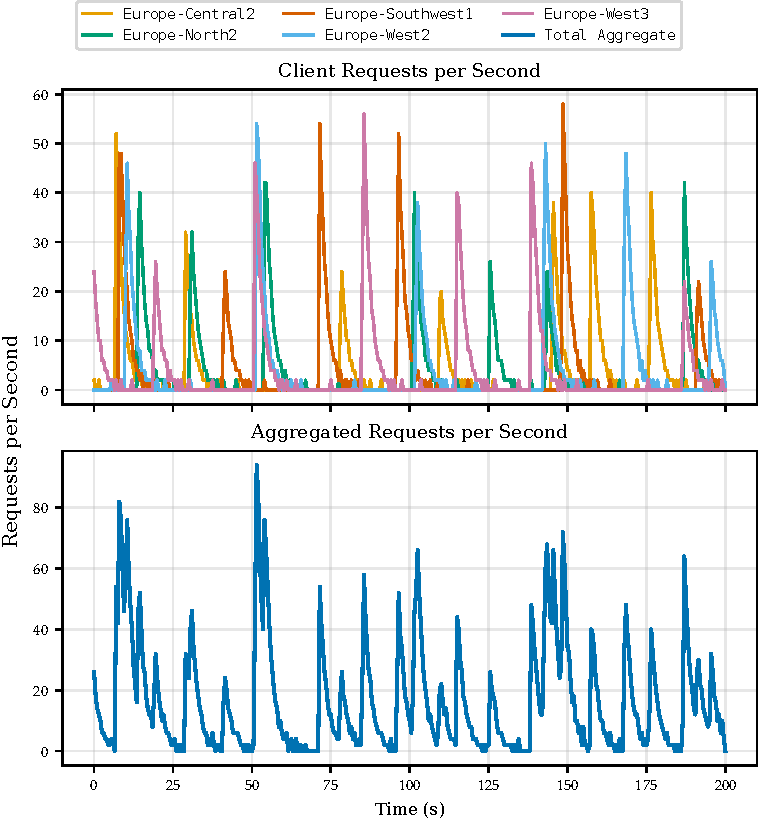
\includegraphics[width=\linewidth]{figures/client_load_localevents.pdf}
    \caption{Sample of the client workload pattern used for experimentation.} 
    \label{fig:workload-pattern}
\end{figure*}

Because the evaluation assesses the viability of an adaptive consensus protocol, the workload must deliberately trigger conditions where the optimal strategy fluctuates between Fast Paxos and Regular Paxos. Under sustained, heavy traffic, standard consensus protocols like OmniPaxos~\cite{Ng-OmniPaxos-2023} or Raft~\cite{Ongaro-Raft-2014} are strictly superior due to high collision rates on the fast path. Consequently, stress-testing maximum throughput is out of scope. Instead, the evaluation employs a highly bursty, low-contention workload to represent ideal conditions for the adaptive system, ensuring periods where the fast path is highly viable are interspersed with periods of high collision risk.

Traffic generation is therefore driven by local events at the clients. To create windows of opportunity for Fast Paxos, the baseline traffic between events is set to zero \gls{RPS}. When a local event triggers at a node, the client injects a rapid burst of 50 peak \gls{RPS}. This simulates a sudden influx of client activity that normalizes along an exponential decay curve with a rate of 0.5. Burst timing is unpredictable: intervals between events are sampled from a normal distribution with a 30-second mean and a 15-second standard deviation. A jitter factor of 0.5 applies randomized variance to the peak height of each burst to further simulate organic traffic.

Each geographic server is driven by a single, independent client process sending requests. This setup does not impact collision rates, as collisions inherently occur across the network between different servers rather than locally. Because each of the nodes generates localized bursts independently, the aggregate system load dynamically fluctuates. Figure \ref{fig:workload-pattern} depicts a sample of this workload pattern, showing both the request trace for individual servers and the overall aggregate load.


\section{Score Function Validity}
\label{sec:score_function_validity}

\section{Risk Guarantee Validity}
\label{sec:risk_guarantee_validity}

\section{Latency Study}
\label{sec:latency_study}

\begin{figure*}[t!]
    \centering
    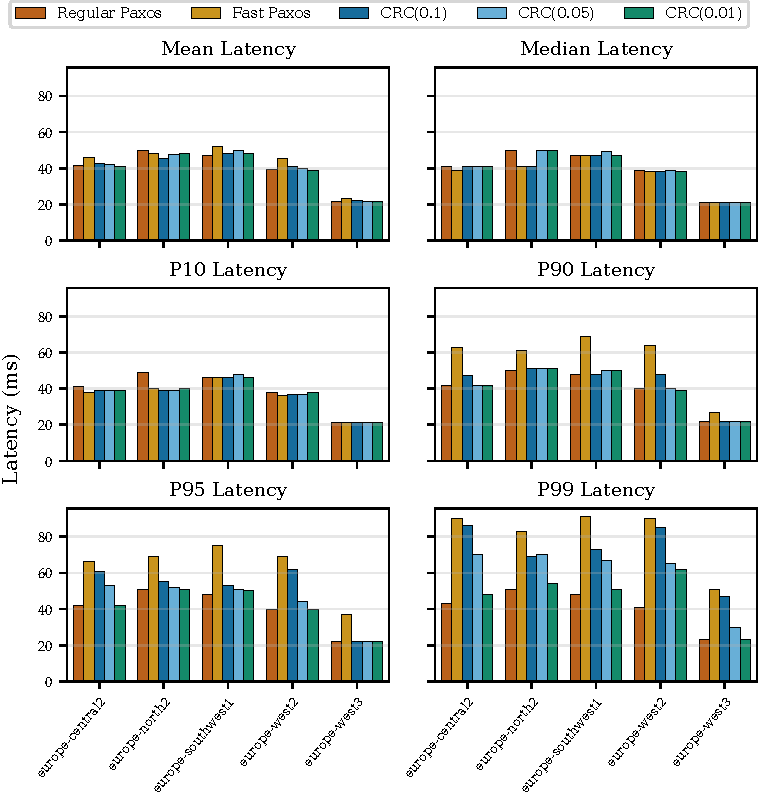
\includegraphics[width=\linewidth]{figures/latency_comparison_europe.pdf}
    \caption{End-to-end latency comparison for the European cluster setup between Regular Paxos, Fast Paxos, and Conformal Consensus with various risk levels.} 
    \label{fig:latency_comparison_europe}
\end{figure*}

We analyze the end-to-end request latencies of Conformal Consensus under different risk levels compared to static Regular Paxos and Fast Paxos baselines. Figures \ref{fig:latency_comparison_europe} and \ref{fig:latency_comparison_us} display the mean, median, and tail latencies (P10, P90, P95, P99) for both regions under the bursty workload pattern described in Section \ref{sec:experimental_setup}.

In the European cluster experiment, Regular Paxos maintains a flat latency profile across all percentiles (P10--P99), demonstrating strong resilience to workload contention. In contrast, static Fast Paxos achieves lower P10 latency for followers but suffers substantial latency inflation at higher percentiles (P90, P95, and P99), producing the widest overall latency spread. This can also be seen at the leader node (\texttt{europe-west3}). Because high-percentile penalties heavily impact the average, static Fast Paxos reduces mean latency only when the geographic fast-path advantage is substantial, as seen at the Stockholm node (\texttt{europe-north2}). Where fast-path benefits are marginal, its mean latency regresses relative to Regular Paxos.

Conformal Consensus dampens these extreme tail latencies. At a conservative risk level ($\alpha = 0.01$), for instance, latency inflation is restricted strictly to the P99 tail and remains unobservable at P90 and P95. Simultaneously, the adaptive mechanism preserves the low P10 latency of Fast Paxos, successfully capturing and increasing mean latency improvements on nodes with large fast-path advantages. However, where fast-path gains are minimal, residual slow-path fallbacks at high percentiles still cause a slight regression in mean latency compared to pure Regular Paxos.

Finally, the target risk level $\alpha$ establishes a direct trade-off between stability and latency reduction. Lowering $\alpha$ systematically increases tail dampening and tightens the overall latency spread toward Regular Paxos, though this added stability proportionally diminishes potential mean latency gains.

\begin{figure*}[t!]
    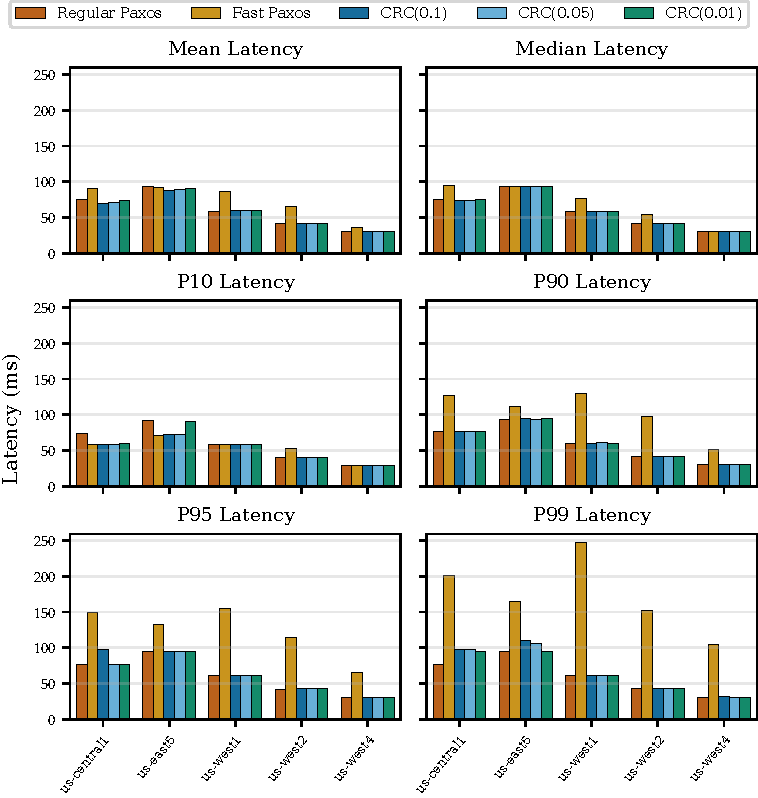
\includegraphics[width=\linewidth]{figures/latency_comparison_us.pdf}
    \caption{End-to-end latency comparison for the (simulated) US cluster setup between Regular Paxos, Fast Paxos, and Conformal Consensus with various risk levels.} 
    \label{fig:latency_comparison_us}
\end{figure*}

To mitigate the unpredictable cloud network variance observed in the US cluster setupc, all nodes were deployed within a single geographic zone (\texttt{us-west4-c}) for the latency experiment, with the regional latency profile injected application-side. Under these conditions, the Regular and Fast Paxos baselines exhibit the same general performance trends observed in the European cluster.

As discussed in Section \ref{sect:node_setup}, the Conformal Consensus configuration continuously routes \texttt{us-west1}, \texttt{us-west2}, and the leader (\texttt{us-west4}) through the regular path. The latencies for these nodes perfectly mirror the Regular Paxos baseline across all percentiles through the added stability. For the actively adapting nodes, higher theoretical fast-path gains result in a noticeable reduction in mean latency, making Conformal Consensus outperform both static baselines in this specific setup.


\section{Overhead Analysis}
\label{sec:overhead_analysis}
Conformal Consensus can introduce overhead in two primary areas: per-request mode evaluation during follower append attempts and threshold computation during batch calibration.

\begin{figure*}[t]
    \centering
    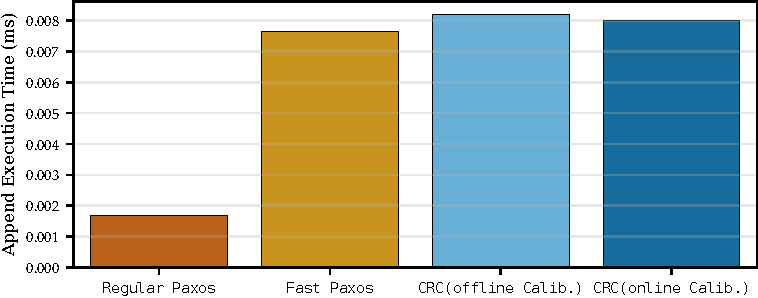
\includegraphics[width=\linewidth]{figures/append_performance.pdf}
    \caption{Average execution times of an append attempt by followers across operating modes.} 
    \label{fig:append_performance}
\end{figure*}

Figure~\ref{fig:append_performance} shows the average local execution time per append attempt on a follower across operating modes. Regular Paxos requires under $0.002\,\text{ms}$ because the follower only forwards incoming requests to the leader. Fast Paxos increases this due to proposal broadcasting among peers. Adding \gls{CRC}, which includes evaluating the heuristic score, generating the prediction set, and processing potential shadow proposals during offline calibration, incurs less than $0.01\,\text{ms}$ of combined compute overhead per request. Given that end-to-end network latencies in both cluster topologies are on the order of tens of milliseconds (Section~\ref{sec:experimental_setup}), this local compute overhead is negligible and has no practical impact on request latency.

\begin{figure*}[t]
    \centering
    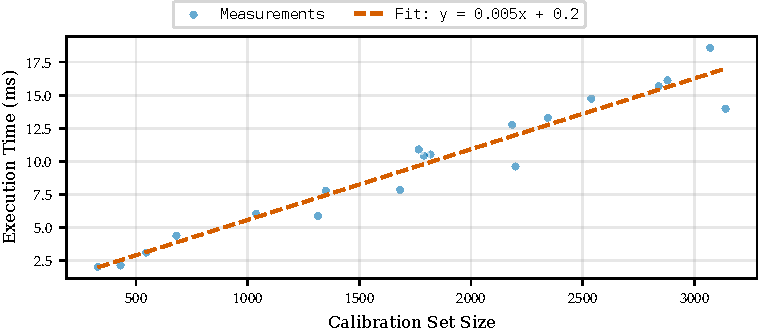
\includegraphics[width=\linewidth]{figures/calibration_overhead.pdf}
    \caption{Threshold computation time during batch calibration relative to calibration set size.} 
    \label{fig:calibration_overhead}
\end{figure*}

The second potential source of overhead is batch calibration, which runs a binary root-finding algorithm to establish an initial threshold $\widehat{\lambda}$. As shown in Figure~\ref{fig:calibration_overhead}, execution time scales linearly with dataset size. For a dataset of 3,000 samples (collected over 15 minutes under described workload patterns), the algorithm computes the threshold in approximately $15\,\text{ms}$. Batch calibration is entirely optional and serves primarily to establish a reliable baseline threshold prior to running online calibration. Because data collection can occur during regular operations, the root-finding routine can execute asynchronously, and the computational load is this low, batch calibration introduces no runtime disruption to the main consensus path.

\cleardoublepage
\chapter{Discussion}
\label{ch:discussion}
\section{Correctness and Validity}

\section{Uncertainty Scores}

\section{Fast Path Viability}

\section{Practical Implications}

\cleardoublepage
\chapter{Conclusions}
\label{ch:conclusionsAndFutureWork}

\section{Conclusions}
\label{sec:conclusions}
\engExpl{Describe the conclusions (reflect on the whole introduction given in Chapter 1).}


  
\engExpl{Discuss the positive effects and the drawbacks.\\
Describe the evaluation of the results of the degree project.\\
Did you meet your goals?\\
What insights have you gained?\\
What suggestions can you give to others working in this area?\\
If you had it to do again, what would you have done differently?}

\sweExpl{Uppfyllde du dina mål?\\
Vilka insikter har du fått?\\
Vilka förslag kan du ge till andra som arbetar inom detta område?
Om du skulle göra detta igen, vad skulle du ha gjort annorlunda?}

\section{Limitations}
\label{sec:limitations}
\engExpl{What did you find that limited your efforts? What are the limitations of your results?}

- Exploratory -> Fundamentally unclear whether a safe and lively version hybrid protocol with log syncing is even achievable

- Struggle with cloud reproducability hindering progress -> final analysis not as exhaustive as could have been

- Only considered if fast-path successful not if faster -> likely the main methological limitation on practicability study ->  guarantees on  end-to-end latency could be more impactful since less prior network layout study is necessary

- No stable storage -> Assumption was that this is not the dominating factor for end-to-end latency in global scenarios but there could be disk I/O overhead for the more complex adaptive version which needs to be considered

- Fixed learning rate of 0.005 for adaptive experiments -> basically just first value stumbled upon in literature \cite{Angelopoulus-NeuralInformationProcessing-2023} -> no study was made regarding its impact (unclear whether there is one) -> batch calibration used as a way to push threshold in the right range from where a low learning rate is acceptable

\section{Future work}
\label{sec:futureWork}

\engExpl{Describe valid future work that you or someone else could or should do.\\
Consider: What you have left undone? What are the next obvious things to be done? What hints can you give to the next person who is going to follow up on your work?}

\begin{itemize}
    \item Fully specify the hybrid protocol with safety and liveness proves to assess whether the approach actually works
    \item Find a way to give guarantees on actual end-to-end latency instead of success since a success does not always mean faster execution -> network latency changes might not impact success when contention is low, but make fast-path execution slower in comparison
    \item Determine a heuristic based on math instead of empirical data seems possible and logical -> worth exploring
    \item Try to integrate the approach into Nezha \cite{Geng-NezhaConsensus-2022}, which makes fast-path more viable
    \item => this work can give guidance on how to approach the problem and how to analyse it
\end{itemize}

\cleardoublepage

\renewcommand{\bibname}{References}

\iftoggle{biblatex}{
    \printbibliography[heading=bibintoc]
}{
    \phantomsection
    \addcontentsline{toc}{chapter}{References}
    \bibliography{references}
}

\cleardoublepage

\appendix

\renewcommand{\chaptermark}[1]{%
    \markboth{Appendix \thechapter\relax:\thinspace\relax#1}{}%
}

\chapter{Proof of Slow-Path Resolution Safety}
\label{seca:slow_path_resolution_safety_proof}
Let $n$ denote the total number of nodes in the cluster, $Q_M = \lceil \frac{n+1}{2} \rceil$ represent the standard majority quorum, and $Q_F = \lceil \frac{3n}{4} \rceil$ represent the fast quorum. Assume the leader has collected $Q_F$ total responses for a given slot. Consider the worst-case scenario where these responses are partitioned entirely between a single value $A$ marked as $\textsc{LeaderAccept}$ and a single value $B$ marked as $\textsc{FastAccept}$. Let $v_A$ and $v_B$ denote the observed vote counts for $A$ and $B$ respectively, such that $v_A + v_B = Q_F$. The number of uncast remaining votes is bounded by $R = n - Q_F$.

For both values to remain viable candidates for quorum satisfaction, the remaining votes must be sufficient to independently drive both values to their respective thresholds. This yields the following system of inequalities:
\begin{align}
    v_A + R &\ge Q_M \label{eq:proof_majority} \\
    v_B + R &\ge Q_F \label{eq:proof_fast}
\end{align}
Summing inequalities (\ref{eq:proof_majority}) and (\ref{eq:proof_fast}) and substituting $v_A + v_B = Q_F$ results in:
\begin{equation}
    Q_F + 2R \ge Q_M + Q_F \implies 2R \ge Q_M
\end{equation}
Substituting $R = n - Q_F$ into the expression yields:
\begin{equation}
    2(n - Q_F) \ge Q_M \implies 2n \ge Q_M + 2Q_F
\end{equation}
By applying the definitions of the quorum thresholds ($Q_M \ge \frac{n+1}{2}$ and $Q_F \ge \frac{3n}{4}$), we obtain:
\begin{equation}
    2n \ge \frac{n+1}{2} + 2\left(\frac{3n}{4}\right) \implies 2n \ge 2n + \frac{1}{2} \implies 0 \ge \frac{1}{2}
\end{equation}
This yields a clear contradiction. Thus, given $Q_F$ total responses, it is mathematically impossible for both value $A$ to retain a path to a standard majority quorum and value $B$ to retain a path to a fast quorum. Consequently, the leader can always unambiguously determine that at least one of the protocol paths has failed to achieve its quorum, allowing for a safe slow-path resolution.

\chapter{Supporting materials}
\label{sec:supportingMaterial}
\generalExpl{Here is a place to add supporting material that can help others build upon your work. You can include files as attachments to the PDF file or indirectly via URLs. Alternatively, consider adding supporting material uploaded as separate files in DiVA.}

% Attach the BibTeX for your references to make it easy for a reader to find and use them
The BibTeX references used in this thesis are attached. \attachfile[description={references.bib}]{references.bib}

% Attach source code file(s) or add a URL to the github or other repository
Some source code relevant to this project can be found at \url{https://github.com/gqmaguirejr/E-learning} and \url{https://github.com/gqmaguirejr/Canvas-tools}.

Your reader can access the attached (embedded) files using a PDF tool such as Adobe Acrobat Reader using the paperclip icon in the left menu, as shown in \Cref{fig:PDFreaderPaperclipExample} or by right-clicking on the push-pin icon in the PDF file and then using the menu to save the embedded file as shown in \Cref{fig:PDFreaderPushpinExample}.

An argument for including supporting material in the PDF file is that it will be available to anyone who has a copy of the PDF file. As a result, they do not have to look elsewhere for this material. This comes at the cost of a larger PDF file. However, the embedded files are encoded into a compressed stream within the PDF file; thus, reducing the number of additional bytes. For example, the references.bib file that was used in this example is \SI{10617}{\byte} in size but only occupies \SI{4261}{\byte} in the PDF file.

\warningExpl{DiVA is limited to $\approx$\SI{1}{\giga\byte} for each supporting file. If you have very large amounts of supporting material, you will probably want to use one of the data repositories. For additional help with this, contact KTH Library via 
\href{mailto:researchdata@kth.se}{researchdata@kth.se}.\\As of Spring 2024, there are plans to migrate this supporting data from DiVA to a research data repository.
}

\begin{figure}[!ht]
  \begin{center}
    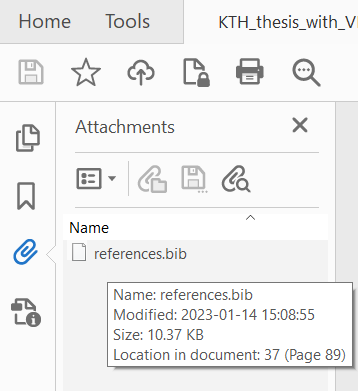
\includegraphics[width=0.50\textwidth]{README_notes/pdf-viewer-attached-files.png}
  \end{center}
  \caption{Adobe Acrobat Reader using the paperclip icon for the attached references.bib file}
  \label{fig:PDFreaderPaperclipExample}
\end{figure}
\FloatBarrier

\begin{figure}[!ht]
  \begin{center}
    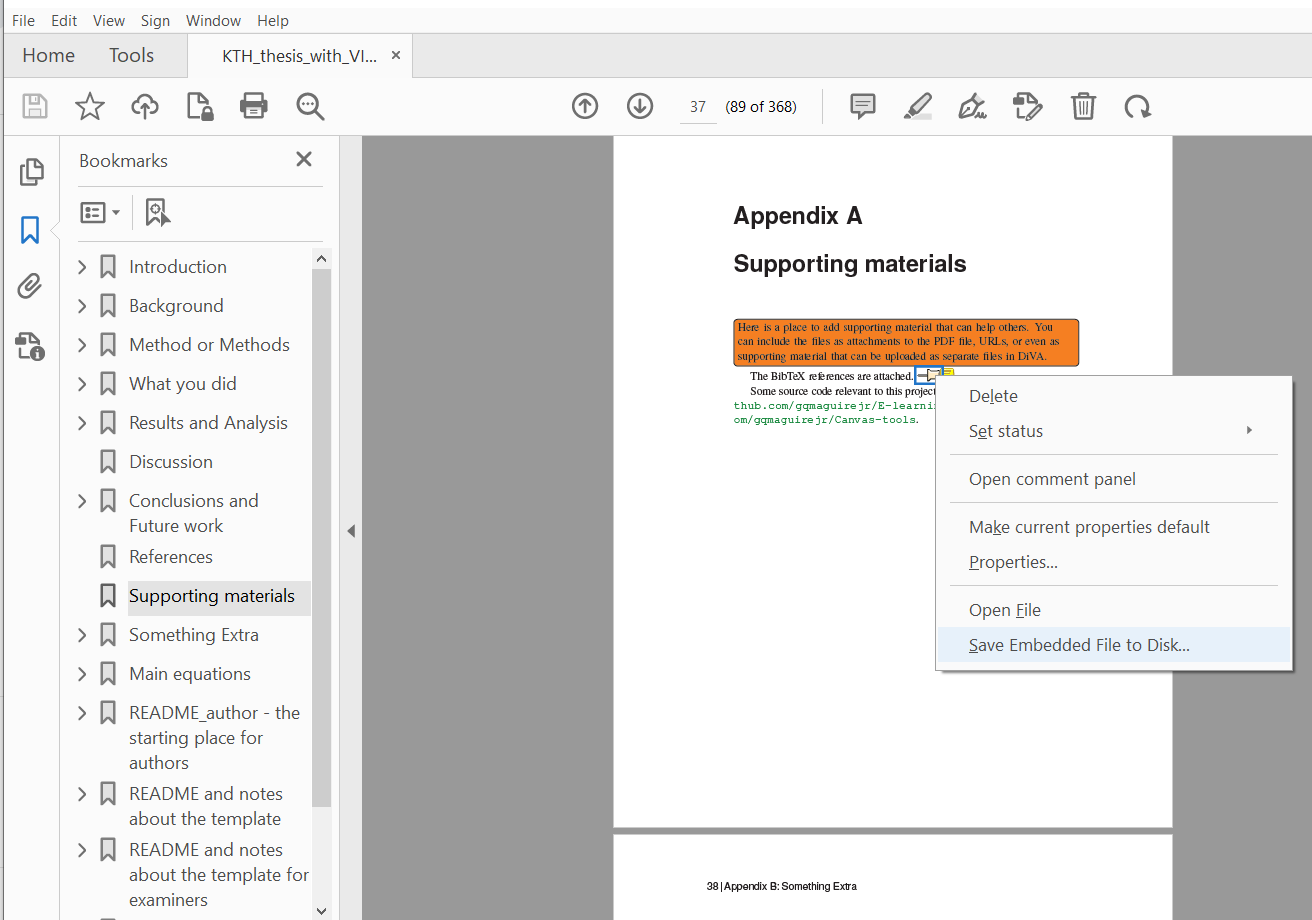
\includegraphics[width=0.99\textwidth]{README_notes/Bib-save-embedded-example.png}
  \end{center}
  \caption{Adobe Acrobat Reader after right-clicking on the push-pin icon for the attached references.bib file}
  \label{fig:PDFreaderPushpinExample}
\end{figure}
\FloatBarrier

%\cleardoublepage
%\chapter{Something Extra}
%\sweExpl{svensk: Extra Material som Bilaga}
%\section{Just for testing KTH colors}
%\iftoggle{digitaloutput}{
    %\textbf{You have selected to optimize for digital output}
%}{
    %\textbf{You have selected to optimize for print output}
%}
%\begin{itemize}[noitemsep]
    %\item Primary color
    %\begin{itemize}
    %\item \textcolor{kth-blue}{kth-blue \iftoggle{digitaloutput}{
    %actually Deep sea
    %}{}} {\color{kth-blue} \rule{0.3\linewidth}{1mm} }\\
    %\item \textcolor{kth-blue80}{kth-blue80} {\color{kth-blue80} \rule{0.3\linewidth}{1mm} }\\
%\end{itemize}
%\item  Secondary colors
%\begin{itemize}[noitemsep]
    %\item \textcolor{kth-lightblue}{kth-lightblue \iftoggle{digitaloutput}{
    %actually Stratosphere
    %}{}} {\color{kth-lightblue} \rule{0.3\linewidth}{1mm} }\\
    %\item \textcolor{kth-lightred}{kth-lightred \iftoggle{digitaloutput}{
    %jactually Fluorescence}{}} {\color{kth-lightred} \rule{0.3\linewidth}{1mm} }\\

    %j\item \textcolor{kth-lightred80}{kth-lightred80} {\color{kth-lightred80} \rule{0.3\linewidth}{1mm} }\\

    %j\item \textcolor{kth-lightgreen}{kth-lightgreen \iftoggle{digitaloutput}{
    %jactually Front-lawn}{}} {\color{kth-lightgreen} \rule{0.3\linewidth}{1mm} }\\

    %j\item \textcolor{kth-coolgray}{kth-coolgray \iftoggle{digitaloutput}{
    %jactually Office}{}} {\color{kth-coolgray} \rule{0.3\linewidth}{1mm} }\\

    %j\item \textcolor{kth-coolgray80}{kth-coolgray80} {\color{kth-coolgray80} \rule{0.3\linewidth}{1mm} }
%j\end{itemize}
%j\end{itemize}

%j\textcolor{black}{black} {\color{black} \rule{\linewidth}{1mm} }

%\cleardoublepage
% Information for authors
%\documentclass[examplethesis.tex]{subfiles}

\begin{document}
\ifxeorlua
\lstdefinestyle{latexExampleForAuthors}{
language=[LaTeX]{TeX},
    breaklines=true,
    postbreak=\mbox{\textcolor{red}{$\hookrightarrow$}\space},
    basicstyle=\small\tt,
    keywordstyle=\color{blue}\sf,
    identifierstyle=\color{magenta},
    commentstyle=\color{cyan},
    backgroundcolor=\color{yellow!15},
    extendedchars=true,
    inputencoding=utf8,
    tabsize=2,
    columns=flexible,
    morekeywords={subtitle, alttitle, altsubtitle, hostcompany, courseCycle,
      courseCode, courseCredits, programcode, degreeName, subjectArea,
      nationalsubjectcategories, todo, ifbiblatex, subsection}
}
\else
\lstdefinestyle{latexExampleForAuthors}{
language=[LaTeX]{TeX},
    breaklines=true,
    postbreak=\mbox{\textcolor{red}{$\hookrightarrow$}\space},
    basicstyle=\small\tt,
    keywordstyle=\color{blue}\sf,
    identifierstyle=\color{magenta},
    commentstyle=\color{cyan},
    backgroundcolor=\color{yellow!15},
    extendedchars=false,
    inputencoding=utf8,
    tabsize=2,
    columns=flexible,
    morekeywords={subtitle, alttitle, altsubtitle, hostcompany, courseCycle,
      courseCode, courseCredits, programcode, degreeName, subjectArea,
      nationalsubjectcategories, todo, ifbiblatex, subsection},
% Support for Swedish, German and Portuguese umlauts
  literate=%
  {Ö}{{\"O}}1
  {Ä}{{\"A}}1
  {Å}{{\AA{}}}1
  {Ü}{{\"U}}1
  {ß}{{\ss}}1
  {ü}{{\"u}}1
  {ö}{{\"o}}1
  {ä}{{\"a}}1
  {å}{{\aa{}}}1
  {á}{{\'a}}1
  {ã}{{\~a}}1
  {é}{{\'e}}1
  {è}{{\`e}}1
  {€}{\euro}1%
  {’}{{\char13}}1
  {-}{{\textendash}}1
  {–}{{\textendash}}1
  {…}{{\ldots}}1,
}
\fi


\chapter{README\_author - the starting place for authors}
\label{ch:READMEauthor}

This chapter describes the thesis template that I (Gerald Q. Maguire Jr.) have developed for use at KTH Royal Institute of Technology (KTH). It is important to note that the template is \textbf{not prescriptive}, as not every thesis will have all of the parts that the template shows. However, if there is something that you decide to leave out, you should make a conscious decision to do so and you should consider the impact this may have on your thesis being approved by the examiner.

Fundamental to the design of the template are several key factors:
\begin{itemize}
    \item Helping students be successful in their degree project,
    \item Helping students produce a high-quality thesis, and
    \item Supporting all of the (relevant) phases of the degree project process.
\end{itemize}

\noindent\textbf{This document is a work in progress.}


\section{Advice for Author or Authors}
\label{sec:authors}
One of the hardest problems an author faces is getting started writing, \ie the blank sheet of paper -- empty file barrier. The template provides a \mbox{non-blank} starting point; hence, avoiding the blank paper barrier. Additionally, the template provides some initial structure, basically, an Introduction, Methods, Results, and Discussion (IMRAD) structure, so that there are hints of where to place material. Moreover, there are places (and notes) about material that the student should consider adding; for example, the ``required reflections'' section in the final chapter.

The template (located in the file \texttt{examplethesis.tex}) also provides some examples of commonly occurring types of content, so that one can easily find examples of how to include a figure, table, code listing, \etc. These examples are not meant to be exhaustive and quite often the student will probably need to learn new \LaTeX\  commands in the course of writing their thesis.

As an author, the first step is to configure the \LaTeX\  engine that you will use to process the files - see \Cref{sec:latexEngine}. The second step will be to configure the template - see \Cref{sec:authorConfigs}. The third step will be to make sure that the information about you, your supervisor(s), and the examiner are correct in the file \texttt{custom\_configuration.tex} - this information uses the macros described in \Cref{sec:authorMacros}. Now that you have a lot of the administrative details taken care of it is time to start to write - see \Cref{sec:startingToWrite}.

Note that if you are using Overleaf:
\begin{description}
    \item[Make your own copy of the template]
    If you have opened the template from a URL, in the upper left-hand corner, click on \textbf{Menu}. Then select \textbf{Copy Project} - this will give you your own private copy.

\item[Use a helpful project name]
    I suggest you include your name in the project name so that when you share it with your supervisor(s) and examiner, they will know it is your project. 
\item[Invite your supervisor(s9 and examiner to your project] 
    You can invite your supervisor(s) and examiner to your project and they can directly comment on and correct your drafts.
\item[Log in to Overleaf with your KTH account] 
If you log in to Overleaf with your KTH account, you get a version of Overleaf that lets you turn on ``Track changes'' which is very useful (particularly if you have invited your supervisor(s) and examiner to join your project). It also gives you a bit more of a time budget to compile (which can be useful if you have a lot of Tikz figures or other things that take a lot of time for the LaTeX engine to render).
\end{description}

.


If you have more detailed questions about the template itself - 
\iflabelexists{ch:READMEnotes}{see \Cref{ch:READMEnotes}.}
{You have to include the \texttt{README\_notes/README\_notes.tex} file when compiling.}

\section{Author configuration of the \LaTeX\  engine}
\label{sec:latexEngine}
The template should work with \textsc{pdfLaTeX}, \XeLaTeX, and \LuaLaTeX.  If you are using Overleaf, I strongly recommend using \XeLaTeX\ ---  as this will get the \texttt{Arial} fonts correct for the KTH cover. If you are running the compiler on your local machine and you use \XeLaTeX\  \textbf{and} you have \texttt{Arial} as a system font, then it will be able to use it. Similarly, for \LuaLaTeX. For \textsc{pdfLaTeX} I have used \textbackslash fontfamily{helvet}, \ie Helvetica, as it is a sans serif font.

One student reported problems with \textsc{fontspec} not loading the fonts properly when running locally with macOS 12.4, TeXLive 2022, LaTeX Workshop on VS Code, and \XeLaTeX\  - the solution is described at \url{https://tug.org/TUGboat/tb39-2/tb122robertson-fontspec.pdf}.

If you are using Overleaf, it is easy to select the compiler (\ie \TeX\ engine) by using the drop-down menu, as shown in \Cref{fig:selectingTeXEngine}.
\begin{figure}[!ht]
  \begin{center}
    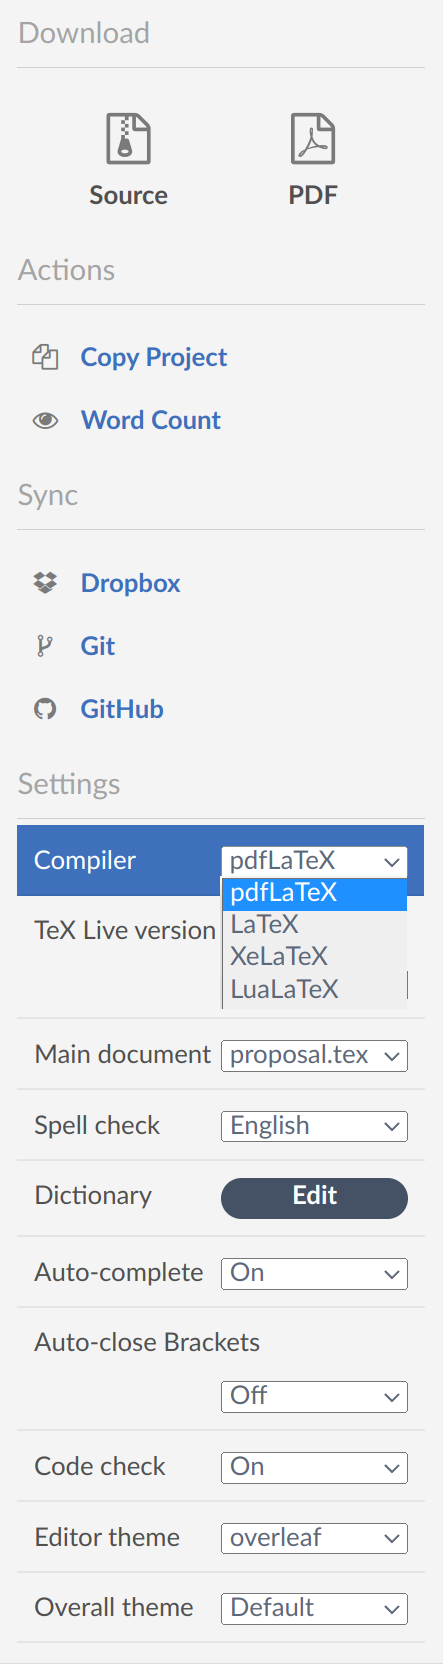
\includegraphics[width=0.40\textwidth]{README_notes/selecting-engine-in-overleaf.png}
  \end{center}
  \caption{Selecting a compiler (\ie TeX engine) in Overleaf}
  \label{fig:selectingTeXEngine}
\end{figure}
\FloatBarrier


\section{Author configuration of the template}
\label{sec:authorConfigs}
The template is designed to handle a thesis written in English or Swedish.
You can set the default language to `english' or `swedish' by passing an option to the documentclass. Note that the language option is written in all lowercase letters; for example, to set the document's language to English:
\begin{lstlisting}[style=latexExampleForAuthors]
\documentclass[english]{kththesis}
\end{lstlisting}

To set the document's language to Swedish (uncomment the following line):
\begin{lstlisting}[style=latexExampleForAuthors]
\documentclass[swedish]{kththesis}
\end{lstlisting}

The language option `swedish' sets the conditional \texttt{\textbackslash ifinswedish} to true.  Among many other things, this conditional is used to configure the KTH cover and the title page to use the chosen language.

The two most common bibliographic engines are supported, \ie BibTeX and BibLaTeX. To set the language to English and use the bibliographic engine to BibTeX you would say:
\begin{lstlisting}[style=latexExampleForAuthors]
\documentclass[english, bibtex]{kththesis}
\end{lstlisting}
To set the language to Swedish and use the bibliographic engine to BibLaTeX you would say:
\begin{lstlisting}[style=latexExampleForAuthors]
\documentclass[swedish, biblatex]{kththesis}
\end{lstlisting}

The above illustrates that you can pass multiple options to the document class separated by commas. Also, note that the options were passed as all lowercase letters.

You can, of course, also modify the formatting of the citations and bibliography. See for example the following code snippet:

\begin{lstlisting}[style=latexExampleForAuthors]
\ifbiblatex
    %\usepackage[language=english,bibstyle=authoryear, citestyle=authoryear, maxbibnames=99]{biblatex}
    %\usepackage[style=numeric,sorting=none,backend=biber]{biblatex}
    \usepackage[bibstyle=authoryear,citestyle=authoryear, maxbibnames=99,language=english]{biblatex}
    % alternatively you might use another style, such as IEEE
    %\usepackage[style=ieee]{biblatex}
    \addbibresource{references.bib}
    %\DeclareLanguageMapping{norsk}{norwegian}
\else
    % The line(s) below are for BibTeX
    \bibliographystyle{bibstyle/myIEEEtran}
    %\bibliographystyle{apalike}
\fi
\end{lstlisting}

To optimize for digital output (this changes the color palette) add the option: \texttt{digitaloutput}. There are also options for A4 or G6 paper: \texttt{a4paper} or \texttt{g5paper} (respectively). The is an option for \texttt{nomenclature}, to produce and refer to equations
\ifnomenclature
as shown in \Cref{ch:NomenclatureExamples}
\fi
.  Finally, there are options for a 1\textsuperscript{st} cycle thesis or 2\textsuperscript{nd} cycle thesis: \texttt{bachelor} and \texttt{master} (respectively); however, these two options are \textbf{not} currently used.

One of the first things that the author(s) will want to do is add the working title and subtitle to the thesis. This is done using the \textbackslash title, \textbackslash subtitle, \textbackslash alttitle, and \textbackslash altsubtitle macros as shown below:
\begin{lstlisting}[style=latexExampleForAuthors]
\title{This is the title in the language of the thesis}
\subtitle{A subtitle in the language of the thesis}

% give the alternative title - i.e., if the thesis is in English,
% then give a Swedish title
\alttitle{Detta är den svenska översättningen av titeln}
\altsubtitle{Detta är den svenska översättningen av undertiteln}
% alternative, if the thesis is in Swedish, then give an English title
%\alttitle{This is the English translation of the title}
%\altsubtitle{This is the English translation of the subtitle}   
\end{lstlisting}

Setting these values once and then using them in many places reduces the work to change them while at the same time ensuring consistency. 

\warningExpl{The issue of what characters can be placed in a title (subtitle, keywords, and abstracts) and how to enter them is a bit complex, but you should be able to achieve much of what you want - at the cost of some effort. Ultimately, the characters that will be placed into DiVA and LADOK must be Unicode, encoded using Unicode Transformation Format (UTF), specifically UTF-8. While DiVA utilizes HTML for these fields, allowing you to include some markup, LADOK does not support any markup.}

\warningExpl{If you have titles or subtitles that cannot be converted to pure Unicode (such as subscripts with capital letters or other symbols), you should also use the optional commands \texttt{\textbackslash titleInPlainText}, \texttt{\textbackslash subtitleInPlainText}, \texttt{\textbackslash alttitleInPlainText}, and \texttt{\textbackslash altsubtitleInPlainText} in your \texttt{custom\_configuration.tex} or \texttt{custom\_configuration\_plaintext.tex} files to provide versions of titles and subtitles that can be used with LADOK. Compiling \texttt{Generate\_titles\_in\_plain\_text.tex} with \textbf{\LuaLaTeX{}} will produce a file named \texttt{extra\_plaintext.tex} containing plain text versions of the \mbox{titles} and subtitles (both main and alternate). The reason that you have to compile using \LuaLaTeX{} is that I have used Lua code and \LuaLaTeX{} to compute the plain text strings. After you have compiled the file, you can follow the workflow to generate, download, edit and merge, and upload the \texttt{custom\_configuration\_plaintext.tex} file to your Overleaf project.}

Some additional configuration that the author(s) might do is to set the values of the macros related to the course cycle, course code, date of the thesis, number of credits, degree/exam name, subject area, and if the degree is done external to KTH to set the host information (see the file \textit{custom\_configuration.text}). Consider the snippet below for a student admitted to the ``Bachelor's Programme in Information and Communication Technology (TCOMK)'' program and enrolled in the degree project course ``IA150X Degree Project in Information and Communication Technology, First Cycle 15.0 credits'' and working at a company ``Företaget AB'':
\begin{lstlisting}[style=latexExampleForAuthors]
\hostcompany{Företaget AB} % Remove this line if the project was not done at a host company

\date{\today}

\courseCycle{1}
\courseCode{IA150X}
\courseCredits{15.0}

\programcode{TCOMK}
\degreeName{Bachelors degree}
% Note that the subject area for a Bachelor's thesis (Kandidatexamen)
% should be either Technology or Architecture
% If the thesis is in Swedish, these would be: teknik | arkitektur
% -- Note the use of lower case for the Swedish subject area
\subjectArea{Technology}
\end{lstlisting}

Note that in the above macros you have to give the English or Swedish names in the arguments to \textbackslash degreeName and \textbackslash subjectArea - as shown below:
\begin{lstlisting}[style=latexExampleForAuthors]
\degreeName{Kandidatexamen}
\subjectArea{teknik}
\end{lstlisting}

For a CDATE student enrolled in the course ``DA231X Degree Project in Computer Science and Engineering, Second Cycle 30.0 credits'', the cycle, program, course code, degree, and subject area information would be:
\begin{lstlisting}[style=latexExampleForAuthors]
\programcode{CDATE}
\courseCycle{2}
\courseCode{DA231X}
\courseCredits{30.0}
\degreeName{Degree of Master of Science in Engineering}
\subjectArea{Computer Science and Engineering}
\end{lstlisting}

The set of possible values for the English or Swedish names in the arguments to \textbackslash degreeName are:
\begin{lstlisting}[style=latexExampleForAuthors]
\degreeName{Higher Education Diploma}
\degreeName{Högskoleexamen}

\degreeName{Bachelors degree}
\degreeName{Kandidatexamen}

\degreeName{Master of Architecture}
\degreeName{Arkitektexamen}

\degreeName{Degree of Master of Science in Engineering}
\degreeName{Civilingenjörs}

\degreeName{Magister}
\degreeName{Magisterexamen}

\degreeName{Degree of Master of Science}
\degreeName{Masterexamen}

\degreeName{Master of Science in Engineering and Master of Arts in Education degree}
\degreeName{Civilingenjör och lärare examen}

\degreeName{Degree of Master of Science in Secondary Education}
\degreeName{Ämneslärarexamen}

\degreeName{Both}		# Degree Project in the Field of Technology <teknikområde> and the Main Field of Study <huvudområde>
\degreeName{Same}		# The case when the field of technology <teknikområde> and main field of study <huvudområde> are the same.
\end{lstlisting}

For the last two cases, the code compares the values of subjectArea and secondSubjectArea.

You can find a list of the program codes and school acronyms in the file:\linebreak[4] \texttt{lib/schools\_and\_programs.ins}.

There are a set of rules about what is to be displayed on the KTH cover. These can be found at \url{https://www.kth.se/social/group/sprakkommitten/page/omrade-for-examensarbete/}.

One of the reasons for many of the macros shown above and below is to collect the information that is needed to report the approved thesis in Digitala Vetenskapliga Arkivet (DiVA) and to report the title(s) and grade in \foreignlanguage{swedish}{Lokalt adb–baserat dokumentationssystem (LADOK)}.

National subject categories are a \textbf{required} field in the DiVA record. These categories follow a definition by \foreignlanguage{swedish}{SCB} (nowadays known as \foreignlanguage{swedish}{Statistikmyndigheten} or in English: Statistics Sweden) and HSV (\foreignlanguage{swedish}{Högskoleverket} - nowadays known as  \foreignlanguage{swedish}{Universitetskanslersämbetet (UK-ämbetet)} and \foreignlanguage{swedish}{Universitets- och högskolerådet (UHR)} or in English: Swedish Higher Education Authority and Swedish Council for Higher Education).
While these codes refer to research areas, these codes are also used in KTH to indicate the area of the thesis. The guidance that I received from the Linköping University library was that one should try to use 5-digit codes when possible. Some examples of these codes are shown in
\Cref{tab:examplesOfnNationalsubjectCategories}.
\begin{description}[leftmargin=!, labelwidth =\widthof{\texttt{\textbackslash nationalsubjectcategories\{\}}}]
\item [\texttt{\textbackslash nationalsubjectcategories\{\}}] comma-separated list of national subject category codes - each a 3 or 5 digit code
\end{description}

\Needspace*{2\baselineskip}
An example for a thesis in Computer Science and Computer Systems:
\begin{lstlisting}[style=latexExampleForAuthors]
\nationalsubjectcategories{10201, 10206}
\end{lstlisting}

You can find examples of the subjects and their codes at in \Cref{tab:examplesOfnNationalsubjectCategories}. The complete list can be found AT \url{https://www.scb.se/contentassets/3a12f556522d4bdc887c4838a37c7ec7/standard-for-svensk-indelning--av-forskningsamnen-2011-uppdaterad-aug-2016.pdf}\\
and\\
\url{https://www.scb.se/contentassets/10054f2ef27c437884e8cde0d38b9cc4/oversattningsnyckel-forskningsamnen.pdf}

You can also find them in \texttt{README\_notes/National\_Subject\_Categories.tex}. This file can be processed separately or included as an appendix by commenting out the begin and end comments around it near the end of the \texttt{examplethesis.tex} file. The full list is about 14 pages long.

\begin{table}[!ht]
  \begin{center}
    \caption{Examples of some national subject categories and their codes}
    \label{tab:examplesOfnNationalsubjectCategories}
    \begin{tabular}{p{0.85cm} L{6.2cm} L{6.2cm}} % <-- Alignments: 1st column left, 2nd middle, with vertical lines in between
      \textbf{Code}  & \textbf{Category (in Swedish)} & \textbf{Category (in English)} \\
      \hline
102 & \foreignlanguage{swedish}{Data- och informationsvetenskap (Datateknik)} &   Computer and Information Sciences \\
      \hline
10201 & \foreignlanguage{swedish}{Datavetenskap (datalogi)} & Computer Sciences \\
      \hline
10202 & \foreignlanguage{swedish}{Systemvetenskap, informationssystem och informatik} (\foreignlanguage{swedish}{samhällsvetenskaplig inriktning} under 50804) &
Information Systems (Social aspects to be 50804)\\
      \hline
10203 & \foreignlanguage{swedish}{Bioinformatik (beräkningsbiologi)} (\foreignlanguage{swedish}{tillämpningar} under 10610) & Bioinformatics (Computational Biology) (applications to be 10610) \\
      \hline
10204 & \foreignlanguage{swedish}{Människa-datorinteraktion (interaktionsdesign)} (\foreignlanguage{swedish}{Samhällsvetenskapliga aspekter} under 50803) & Human Computer Interaction (Social aspects to be 50803)\\
      \hline
10205 & \foreignlanguage{swedish}{Programvaruteknik} & Software Engineering \\
      \hline
10206 & \foreignlanguage{swedish}{Datorteknik} & Computer Engineering \\
      \hline
10207 & \foreignlanguage{swedish}{Datorseende och robotik (autonoma system) }& Computer Vision and Robotics (Autonomous Systems) \\
      \hline
10208 & \foreignlanguage{swedish}{Språkteknologi (språkvetenskaplig databehandling)} & Language Technology (Computational Linguistics) \\
      \hline
10209 & \foreignlanguage{swedish}{Medieteknik} & Media and Communication Technology \\
      \hline
10299 & \foreignlanguage{swedish}{Annan data- och informationsvetenskap} & Other Computer and Information Science \\
      \hline
      \hline
202   & \foreignlanguage{swedish}{Elektroteknik och elektronik} & Electrical Engineering, Electronic Engineering, Information Engineering \\
      \hline
20201 & \foreignlanguage{swedish}{Robotteknik och automation} & Robotics \\
      \hline
20202 & \foreignlanguage{swedish}{Reglerteknik} & Control Engineering \\
      \hline
20203 & \foreignlanguage{swedish}{Kommunikationssystem} & Communication Systems \\
      \hline
20204 & \foreignlanguage{swedish}{Telekommunikation} & Telecommunications \\
      \hline
20205 & \foreignlanguage{swedish}{Signalbehandling} & Signal Processing \\
      \hline
20206 & \foreignlanguage{swedish}{Datorsystem} & Computer Systems \\
      \hline
20207 & \foreignlanguage{swedish}{Inbäddad systemteknik} & Embedded Systems \\
      \hline
20299 & \foreignlanguage{swedish}{Annan elektroteknik och elektronik} & Other Electrical Engineering, Electronic Engineering, Information Engineering \\
      \hline
    \end{tabular}
  \end{center}
\end{table}


\FloatBarrier
\clearpage
\Needspace*{10\baselineskip}
\subsection{Setting the UN's Sustainable Development Goals (SDGs) information}
The UN's Sustainable Development Goals (SDGs) are a field in the DiVA record.
Some examples of these SDGs are shown in Table~\ref{tab:SDGcodes}.
\begin{description}[leftmargin=!, labelwidth =\widthof{\texttt{\textbackslash nationalsubjectcategories\{\}}}]
\item [\texttt{\textbackslash SDGs\{\}}] comma-separated list of SDG codes - each a numerical value
\end{description}

\Needspace*{2\baselineskip}
An example of a thesis supporting SDGs 8 and 9:
\begin{lstlisting}[style=latexExampleForAuthors]
\SDGs{8, 9}
\end{lstlisting}

%% UN's Sustainable Development Goals (SDGs)
% sdg1	eng: No poverty, swe: Ingen fattigdom
% sdg2	eng: Zero hunger, swe: Ingen hunger
% sdg3	eng: Good health and well-being, swe: God hälsa och välbefinnande
% sdg4	eng: Quality education, swe: God utbildning för alla
% sdg5	eng: Gender equality, swe: Jämställdhet
% sdg6	eng: Clean water and sanitation, swe: Rent vatten och sanitet för alla
% sdg7	eng: Affordable and clean energy, swe: Hållbar energi för alla
% sdg8	eng: Decent work and economic growth, swe: Anständiga arbetsvillkor och ekonomisk tillväxt
% sdg9	eng: Industry, innovation and infrastructure, swe: Hållbar industri, innovationer och infrastruktur
% sdg10	eng: Reduced inequalities, swe: Minskad ojämlikhet
% sdg11	eng: Sustainable cities and communities, swe: Hållbara städer och samhällen
% sdg12	eng: Responsible consumption and production, swe: Hållbar konsumtion och produktion
% sdg13	eng: Climate action, swe: Bekämpa klimatförändringarna
% sdg14	eng: Life below water, swe: Hav och marina resurser
% sdg15	eng: Life on land, swe: Ekosystem och biologisk mångfald
% sdg16	eng: Peace, justice and strong institutions, swe: Fredliga och inkluderande samhällen
% sdg17	eng: Partnerships for the goals, swe: Genomförande och globalt partnerskap

\begin{table}[!ht]
  \begin{center}
    \caption{UN's Sustainable Development Goals (SDGs)}
    \label{tab:SDGcodes}
    \begin{tabular}{p{0.85cm} L{6.0cm} L{6.0cm}} % <-- Alignments: 1st column left, 2nd middle, with vertical lines in between
      \textbf{SDG}  & \textbf{Category (in English)} & \textbf{Category (in Swedish)} \\
      \hline
1 & No poverty& \foreignlanguage{swedish}{Ingen fattigdom} \\ \hline
2 & Zero hunger& \foreignlanguage{swedish}{Ingen hunger} \\ \hline
3 & Good health and well-being& \foreignlanguage{swedish}{God hälsa och välbefinnande} \\ \hline
4 & Quality education& \foreignlanguage{swedish}{God utbildning för alla} \\ \hline
5 & Gender equality& \foreignlanguage{swedish}{Jämställdhet} \\ \hline
6 & Clean water and sanitation& \foreignlanguage{swedish}{Rent vatten och sanitet för alla} \\ \hline
7 & Affordable and clean energy& \foreignlanguage{swedish}{Hållbar energi för alla} \\ \hline
8 & Decent work and economic growth& \foreignlanguage{swedish}{Anständiga arbetsvillkor och ekonomisk tillväxt} \\ \hline
9 & Industry, innovation and infrastructure& \foreignlanguage{swedish}{Hållbar industri, innovationer och infrastruktur} \\ \hline
10 & Reduced inequalities& \foreignlanguage{swedish}{Minskad ojämlikhet} \\ \hline
11 & Sustainable cities and communities& \foreignlanguage{swedish}{Hållbara städer och samhällen} \\ \hline
12 & Responsible consumption and production& \foreignlanguage{swedish}{Hållbar konsumtion och produktion} \\ \hline
13 & Climate action& \foreignlanguage{swedish}{Bekämpa klimatförändringarna} \\ \hline
14 & Life below water& \foreignlanguage{swedish}{Hav och marina resurser} \\ \hline
15 & Life on land& \foreignlanguage{swedish}{Ekosystem och biologisk mångfald} \\ \hline
16 & Peace, justice and strong institutions& \foreignlanguage{swedish}{Fredliga och inkluderande samhällen} \\ \hline
17 & Partnerships for the goals& \foreignlanguage{swedish}{Genomförande och globalt partnerskap} \\ \hline
\end{tabular}
  \end{center}
\end{table}

\FloatBarrier

\section{Author macros}
\label{sec:authorMacros}
It is assumed that there can only be 1 or 2 authors. For many years now 2\textsuperscript{nd} cycle theses are expected to only have one author.

For the author or first author, there are a number of macros defined to store information about the author, so that it can later be used in multiple places -- for example, the KTH cover (produced with \texttt{\textbackslash kthcover)}, the title page (via \texttt{\textbackslash titlepage}, the ``For DIVA'' section at the end of the thesis (via
\texttt{\footnotesize\textbackslash divainfo\{pg:lastPageofPreface\}\{pg:lastPageofMainmatter\}}), and possibly a JavaScript Object Notation (JSON) file named \texttt{fordiva.json} produced as a by product of the \texttt{\textbackslash divainfo}. Note that the actual section name has DiVA set in all caps - which hopefully should not occur in the thesis! If the string DiVA set in all caps, does have to appear, then the section heading should be preceded by four euro signs and followed by four more euro signs (as is done in this document).

The author-related macros are:
\begin{description}[leftmargin=!, labelwidth =\widthof{\texttt{\textbackslash secondAuthorsFirstname\{\}}}]
\item [\texttt{\textbackslash authorsLastname\{\}}] the last name of the author\footnote{Note that the author's name can include a suffix such as ``, Jr.'' or `` Jr.'', i.e., the suffix can be separated with a comma or not -- as the author prefers to write their name.}

\item [\texttt{\textbackslash authorsFirstname\{\}}] the first name of the author

\item [\texttt{\textbackslash email\{\}}] the KTH e-mail address of the author

\item [\texttt{\textbackslash kthid\{\}}] the author's kthid, this generally starts with the string ·``u1'' and is a unique identifier for every KTH user.

% As per email from KTH Biblioteket on 2021-06-28 students cannot have an OrCiD reported for their degree project
\item [\texttt{\textbackslash authorsSchool\{\}}] the value is generally of the form:\linebreak[4] \texttt{\textbackslash schoolAcronym\{XXX\}}. The\linebreak[4] currently supported school acronyms are: ABE, CBH, EECS, ITM, and SCI. These are defined in the file\linebreak[4] \texttt{schools\_and\_programs.ins}. There is also a fake school XXX for use in the template.
\end{description}

If the first author is not in Stockholm, Sweden when the acknowledgements are written, then add that information via the macros described below.
This information will be used when generating the acknowledgements signature. The acknowledgements signature is the text at the end of the acknowledgements and it gives the place where the author(s) is/are when writing the acknowledgements and also gives the date and name(s).
\begin{description}[leftmargin=!, labelwidth =\widthof{\texttt{\textbackslash secondAuthorsFirstname\{\}}}]
\item [\texttt{\textbackslash authorCity\{A City\}}] specify the city

\item [\texttt{\textbackslash authorCountry\{A Country\}}] specify the country

\item [\texttt{\textbackslash authorCityCountryDate\{\}}] pass into this function the month and year for the acknowledgement. This can be a string such as January 2022 or it can be a \LaTeX\  expression, such as \textbackslash MONTH\textbackslash enspace\textbackslash the\textbackslash year.
\end{description}

If there is a second author and the place, month, and year are \textbf{all} the same, then specify the month and year for only the \textbf{first} author:
\begin{lstlisting}[style=latexExampleForAuthors]
\authorCityCountryDate{\MONTH\enspace\the\year}
\end{lstlisting}

If there is a second author and the place is different, then say:
\begin{lstlisting}[style=latexExampleForAuthors]
\authorCityCountryDate{}
\end{lstlisting}
%\clearpage

If there is a second author, the macros are:
\begin{description}[leftmargin=!, labelwidth =\widthof{\texttt{\textbackslash secondAuthorsFirstname\{\}}}]
\item [\texttt{\textbackslash secondAuthorsLastname\{\}}] the last name of the 2\textsuperscript{nd} author
\item [\texttt{\textbackslash secondAuthorsFirstname\{\}}] the first name of the 2\textsuperscript{nd} author
\item [\texttt{\textbackslash secondemail\{\}}] the KTH e-mail address of the 2\textsuperscript{nd} author
\item [\texttt{\textbackslash secondkthid\{\}}] the 2\textsuperscript{nd} author's kthid
% As per email from KTH Biblioteket on 2021-06-28 students cannot have an OrCiD reported for their degree project
\item [\texttt{\textbackslash secondAuthorsSchool\{\}}] the school of the 2\textsuperscript{nd} author
\end{description}

If the second author is not in the same place as the first author, then add the relevant information using the macros below.  This information will be used when generating the acknowledgements signature.
\begin{description}[leftmargin=!, labelwidth =\widthof{\texttt{\textbackslash secondAuthorsFirstname\{\}}}]
\item [\texttt{\textbackslash secondAuthorCity\{A City\}}]  specify the city

\item [\texttt{\textbackslash secondAuthorCountry\{A Country\}}] specify the country

\item [\texttt{\textbackslash secondAuthorCityCountryDate\{\small\textbackslash MONTH\textbackslash enspace\textbackslash the\textbackslash year\}}]  pass into this function the month and year for the acknowledgement
\end{description}

If the second author is the same place as the first author, then comment out or delete the \textbackslash secondAuthorCityCountryDate\{\} as shown below:
\begin{lstlisting}[style=latexExampleForAuthors]
%\secondAuthorCityCountryDate{}
\end{lstlisting}

\section{Starting to write - for the impatient}
\label{sec:writingForTheImpatient}
For those who are impatient and rapidly want to start writing, I suggest you start by configuring the \texttt{custom\_configuration.tex} file (see \Cref{sec:authorConfigs}), your working title, and abstract (\Cref{sec:wrtingFirstAbstract}). After this, a quick way to start writing the text in your document is to go to the table of contents in Overleaf and click on a chapter or section - this will utilize a hyperlink to go to that part of the PDF file. Next, click on the left-going arrow near the top of the border between the LaTeX on the left and the PDF on the right; this will take you (close) to the correct place in the source file where you can start to modify the content and write.

\section{Starting to write}
\label{sec:startingToWrite}


As you write you will notice "todo" notes in the template. They follow the following conventions:
\begin{lstlisting}[style=latexExampleForAuthors]
\generalExpl{Comments/directions/... in English}
\sweExpl{Text på svenska}
\engExpl{English descriptions about formatting}
\sweExpl{warnings}
\end{lstlisting}

If you do not want to see these notes, you can, of course, redefine the above macros to output nothing. If you do not want to see any notes, then add the option \textbf{final} to the \textbackslash documentclass arguments near the top of the file \texttt{examplethesis.tex}.

\subsection{Working abstract}
\label{sec:wrtingFirstAbstract}
I generally recommend that every student start by writing a working abstract, this will help you keep your focus. To find where you can start to enter your abstract, look in the \texttt{examplethesis.tex} file for the line:
\begin{lstlisting}[style=latexExampleForAuthors]
\generalExpl{Enter your abstract here!}
\end{lstlisting}

There is lots of information already in the template to help you with entering text, equations, \etc in your abstract. \textbf{NB} Abstracts are supposed to stand by themselves, this means no footnotes, no cross-references, no figures, no tables, \etc.

I suggest avoiding the use of the defined acronyms in abstracts \ie spell them out rather than using the glossary commands. This is due to the fact that the \texttt{glossaries} package (that is being used to support acronyms) does not directly provide support for multiple languages and because I do not understand how to programmatically create plurals of acronyms in Swedish or other languages. Even in an English abstract, it is desirable to avoid using the glossary commands - as this makes subsequent processing of the abstracts harder - since one has to make sure that the list of acronyms and their definitions are provided to any program that will process this \LaTeX\  source code. For this reason, later versions of this template include the acronyms.tex file after the metadata for DiVA.

\subsection{Structure of the abstracts and summaries}
The basic \LaTeX\  structure for an abstract or summary is shown below (for the case of an English abstract and a Swedish summary \ie sammanfattning):
\begin{lstlisting}[style=latexExampleForAuthors]
\begin{abstract}
  \markboth{\abstractname}{}
\begin{scontents}[store-env=lang]
eng
\end{scontents}

\begin{scontents}[store-env=abstracts,print-env=true]
here is where you abstract goes.
\end{scontents}

\subsection*{Keywords}
\begin{scontents}[store-env=keywords,print-env=true]
% If you set the EnglishKeywords earlier, you can retrieve them with:
\InsertKeywords{english}
% If you did not set the EnglishKeywords earlier then simply enter the comma separate keywords here:
%such as: Canvas Learning Management System, Docker containers, Performance tuning
\end{scontents}
\end{abstract}

\cleardoublepage
\babelpolyLangStart{swedish}
\begin{abstract}
    \markboth{\abstractname}{}
\begin{scontents}[store-env=lang]
swe
\end{scontents}
\begin{scontents}[store-env=abstracts,print-env=true]
Swedish summary goes here
\end{scontents}
\subsection*{Nyckelord}
\begin{scontents}[store-env=keywords,print-env=true]
% SwedishKeywords were set earlier, hence we can use alternative 2
\InsertKeywords{swedish}
\end{scontents}
\end{abstract}
\babelpolyLangStop{swedish}
\end{lstlisting}

It is important to note that the contents of the \texttt{scontents} environment for the abstracts are stored \textbf{verbatim}, \ie the \LaTeX\  is \textbf{not} executed. The reason for this is to be able to later have a program that can manipulate the source \LaTeX\  to convert it to HTML for use in announcements, calendar events, and for DiVA. This means that if you write the following:
\begin{lstlisting}[style=latexExampleForAuthors]
\begin{scontents}[store-env=abstracts,print-env=true]
\input{abstract.txt}
\end{scontents}
\end{lstlisting}
\noindent what will end up in your abstract in the metadata save for DiVA will simply be: \texttt{''\textbackslash input\{abstract.tex\}''} -- which means that someone will have to cut and paste your actual abstract to insert it into DiVA.

It is also important to note that that the following lines:
\begin{lstlisting}[style=latexExampleForAuthors]
\begin{scontents}[store-env=lang]
eng
\end{scontents}
\end{lstlisting}
\noindent \textbf{must} be before the \texttt{scontents} environment for the abstracts and keywords -- as these lines indicate what language the subsequent abstract and keywords are in. The three-character code used for the language is the ISO 639-2 Code – specifically the "B" (bibliographic) variant of these codes --- as these codes are used in the DiVA metadata to tag what language is used.

\subsection{Abstracts must be able to stand alone}
\label{sec:standaloneAbstract}

The abstract needs to be able to stand alone; therefore, you \textbf{cannot} include citations to your references -- as the references are \textbf{not} part of the abstract! It is possible (but very rare) to have footnotes as part of the abstract. However, you should be aware that quite often, if the abstract is manually entered in DiVA, the footnote might not be entered. In this case, unless your full text is available (\eg via DiVA), a reader might not have an easy way to find out what the footnote says.

\subsection{Acronyms}
\label{sec:addingAcronyms}
You may want to define an acronym to help you with your writing, as this can both reduce the amount of typing and help your reader by providing consistent use of acronyms. The acronyms' definitions can be found in the file \textit{lib/acronyms.tex}. The file contains some examples. I generally try to sort the lines to help find which acronyms I already have defined and keep track of the new one(s) I want to add.

\subsection{Some predefined macros to help when writing}
\label{sec:predefine}

The file \textit{lib/defines.tex} includes some macros that will help you when writing. This includes \textbackslash etc, to give you ``\etc'', \textbackslash eg, \textbackslash ie, and \textbackslash etal.
The file also defines \textbackslash first, \textbackslash Second, ... \textbackslash eighth to give you \first, \Second, \third, ... \eighth. Note that `Second' is written with an initial capital letter to avoid conflict with the unit `second' in the \texttt{siunitx} package.

\subsection{Additional abstract(s)}
\label{sec:additionalAbstracts}

All theses at KTH are \textbf{required} to have an abstract in both \textit{English} and \textit{Swedish}. However, in addition to this, many students want to add abstracts in additional languages. The template comes pre-configured with places for abstracts in several other languages. If there is a language that you want to use that is not already supported, there are directions for how to add an additional language. If there are abstracts in languages that you do not want, please delete them or comment them out (see \Cref{sec:hideComment}).

\subsection{Removing and hiding parts that you do not want}
\label{sec:hideComment}

It is quite likely that you will find parts of the template that you do not want/need. One way of dealing with this is to delete them, and another way is to comment them out. Personally, I like to comment things out, in case I actually do want to be able to read it in the \LaTeX\  file or uncomment it later. To comment out a portion of the file, simply use the following environment:

\begin{lstlisting}[style=latexExampleForAuthors]
\begin{comment}
    **** what you want to comment out ****
\end{comment}
\end{lstlisting}

For example, if you are not interested in the Swedish language \texttt{todo} notes, you can look for lines with ``\textbackslash sweExpl'' in them and comment them out (or delete them).

\subsection{Removing the README\_notes}
At some point you will no longer want this README information. You can remove it by removing the line
\textbackslash include\{README\_notes/README\_notes\} -- from the \textit{examplethesis.tex} file. You can then remove the \textbf{README\_notes} directory.

Unless you are an examiner or an administrator you can delete the file: \texttt{README\_notes/README\_examiner\_notes.tex} and delete the include of this file from near the end of the template (\ie \textit{examplethesis.tex}. You can also delete the directory \textbf{README\_notes/README\_examiner-figures}.


\section[Copyright or Creative Commons License]{Copyright or Creative Commons\\ License}
\label{sec:copyrightOrCClicense}
It is possible to have several variants of the bookinfo page\footnote{When printed double sided, the bookinfo page is the back of the title page.}:
\begin{enumerate}[labelwidth =\widthof{\textbf{Creative Commons (CC)}}, leftmargin = !]
    \item[copyright] If you want to have a bookinfo page, include the line saying \textbackslash bookinfopage.
    \item[Creative Commons (CC)] If you want to have a bookinfo page but want to have a Creative Commons license, then include \textbackslash bookinfopage and use and configure the \texttt{doclicense} package as described below.
    \item[none] If you do \textbf{not} want to have a bookinfo page, comment the line saying \textbackslash bookinfopage and add a \textbackslash cleardoublepage.
\end{enumerate}

For background about Creative Commons licenses, see:
\url{https://www.kb.se/samverkan-och-utveckling/oppen-tillgang-och-bibsamkonsortiet/open-access-and-bibsam-consortium/open-access/creative-commons-faq-for-researchers.html} and \url{https://kib.ki.se/en/publish-analyse/publish-your-article-open-access/open-licence-your-publication-cc}.

Note that the lowercase version of the Creative Commons license has to be used in the modifier, \ie one of: by, by-nc, by-nd, by-nc-nd, by-sa, by-nc-sa, or zero. For the list of supported licenses, see the documentation for the \texttt{doclicense} package.

Note that if the \texttt{doclicense} package is used, it automatically redefines \texttt{\textbackslash bookinfopage} to be \texttt{\textbackslash bookinfopageCC}.

\subsection{Example configuration to have a CC BY-NC-ND license}

\begin{lstlisting}[style=latexExampleForAuthors]
\usepackage[
    type={CC},
    modifier={by-nc-nd},
    version={4.0},
    hyphenation={RaggedRight},
]{doclicense}
\end{lstlisting}

Note that the option ``hyphenation={RaggedRight}'' can be used with the configuration of the package to set the license information with a ragged right margin rather that as a filled and justified paragraph.


\subsection{Example configuration to have a CC BY-NC-ND license with a Euro symbol rather than a Dollar sign}

\begin{lstlisting}[style=latexExampleForAuthors]
\usepackage[
    type={CC},
    modifier={by-nc-nd},
    version={4.0},
    imagemodifier={-eu-88x31},  % to get Euro symbol rather than Dollar sign
    hyphenation={RaggedRight},
]{doclicense}
\end{lstlisting}


\subsection{Example configuration to have a CC0 license}

\begin{lstlisting}[style=latexExampleForAuthors]
\usepackage[
    type={CC},
    modifier={zero},
    version={1.0},
]{doclicense}
\end{lstlisting}

\section{Use of fonts within the thesis}
\label{sec:useOfFontsWithinThesis}

The choice of fonts is a very individual matter and may be affected by the kind of content that you are trying to write, the language that you are writing in, and what you want to convey to your reader. However, some points to keep in mind are:
\begin{itemize}
    \item Use fonts with serifs for the body of your thesis, their presence makes it much easier for your reader.

    \item Use sans serif fonts for headings. This helps your reader distinguish them from the body.

    \item Be very careful when using fonts that are not widely available\footnote{For example, even though it is widely used. not everyone has the Arial font. Additionally, it is a proprietary font; thus, you need to have an appropriate license to use it.}. Unless you embed the fonts that you have used, your readers may not see what you want them to see. Ideally, you should embed all fonts -- even if you only embed the subset you use.

    \item Although there are fonts that have a huge number of characters in them, they might not have the characters that you need.

    \item There are also fonts that, although they have a vast number of characters in them, do not have the math table that \LaTeX\ needs to be able to set mathematical content\footnote{An example of such a font is Google's Noto font. Even though it includes a vast number of characters, it lacks a math table -- although there is an awareness of this missing feature}.

    \item Many fonts are proprietary, thus you need to consider whether you have an appropriate license to use them.
\end{itemize}

What can you do when the fonts you use are missing characters that you need to use? One solution is to use a font that has the character(s) that you want and then make use of them in the places that you need to.

\warningExpl{The details of working with different fonts and characters is a rather complex area and not for the faint-hearted. However, if you \textbf{really} want to have specific characters, \XeLaTeX\ and \LuaLaTeX\ have the means to help you realize what you want. }

\section{One big thesis file or a master file with includes of the parts}
\label{sec:onebigFIlevsincludes}

While many students split their thesis into multiple files (such as\linebreak[4] \texttt{introduction.tex}, \texttt{background.tex}, \texttt{method.tex}, \linebreak[4]\texttt{what-you-did.tex}, \texttt{results-and-analysis.tex},\linebreak[4] \texttt{discussion.tex}, \texttt{conclusion-and-future-work.tex}) and then include these in their main document (with a series of \textbackslash include{xxxx}), my experience is that it actually makes it hard to be consistent in the thesis. For example, you cannot do a simple global replacement when you have decided to introduce a particular acronym. It also makes searching for things difficult, as Overleaf's search function only works on individual files\footnote{Note that this is not a problem if you use emacs and a tags file, as this can do searching over the whole set of files and even a tags based query and replace.}. Personally, I find it hard to correct LaTeX errors when the file is split in this way - since Overleaf does not make it simple to find the root cause of a problem when the chapters are included in this way. There can be a problem with compiling the project in Overleaf, as Overleaf doe not always handle the separate files as one document (unless you use the functions to tell LaTeX that a file is part of a larger document and identify the parent document). Although I have had some students do this splitting successfully and they liked being able to compile just a part of their report; I've personally had strange errors occur with it - hence I did not use this with the template.


There are some advantages to splitting the document into different parts:
\begin{itemize}
\item    Overleaf has a limit on the number of changes that it can track - but this limit is per file!  [Yes, I have gotten bitten by this when I have put in more changes and comments than the limit and had to stop marking up  a manuscript.]

\item    Additionally, Overleaf has a per file size limit (\ie how large a file can be) - again this is per file [Yes, I have gotten bitten by this when exporting a Jupyter notebook that produced a LaTeX file larger than \SI{50}{\mega\byte}.]

\item    This is useful when different students (in a 1st cycle degree project) are writing different parts of the report (in this case the divisions can be even at the section or subsection level).
\end{itemize}

Similarly, many students like to group their figures along with their chapters, \ie introducing a folder for each part of the report and placing both the text and the figures relevant to this section into the relevant folder. A similar approach can be used with included code snippets, tables, \etc.

Ultimately, I think the main issue is the degree to which the separate files are separate and can be worked on as if they were very independent. This generally is true in third-cycle theses, as the chapters tend to be rather independent - typically with one conference/journal paper as the focus of a chapter. However, my experience is that first-cycle theses have very highly interdependent parts, while 2\textsuperscript{nd} cycle theses are split between highly interdependent and highly independent.

However, some might find the question of splitting or not to be a matter of taste or perhaps different ways to approach organizing their writing. So you and your supervisor(s) and examiners might want to discuss what choice is most suitable for your purposes.


\end{document}

%\subfile{README_author}

%\cleardoublepage
% information about the template for everyone
%% This README demonstrates the ability to have a separate glossary for a chapter/appendix

% \newacronym[⟨options⟩]{⟨label⟩}{⟨abbrv⟩}{⟨long⟩}
%\newglossaryentry{⟨label⟩}{type=\acronymtype,
%name={⟨abbrv⟩},
%description={⟨long⟩},
%text={⟨abbrv⟩},
%first={⟨long⟩ (⟨abbrv⟩)},
%plural={⟨abbrv⟩s},
%firstplural={⟨long⟩s (⟨abbrv⟩s)},
%⟨options⟩}



\lstdefinestyle{latexExample}{
language=[LaTeX]{TeX},
    breaklines=true,
    postbreak=\mbox{\textcolor{red}{$\hookrightarrow$}\space},
    basicstyle=\small\tt,
    keywordstyle=\color{blue}\sf,
    identifierstyle=\color{magenta},
    commentstyle=\color{cyan},
    backgroundcolor=\color{yellow!15},
    tabsize=2,
    columns=flexible,
}
\lstset{style=latexExample}
\newcommand{\dname}[1]{\textbf{#1}}
\newcommand{\fname}[1]{\texttt{#1}}

\chapter{README and notes about the template}
\label{ch:READMEnotes}

\glsresetall[readme]
This document, written by Gerald Q. Maguire Jr,  describes the thesis template that I have developed for use at \gls{KTH} and provides some background about why it is the way that it is. It is important to note that the template is \textbf{not prescriptive}, as not every thesis will have all the parts the template shows. However, if there is something that you decide to leave out, you should make a conscious decision to do so, and you should consider the impact this may have on your thesis being approved by the examiner.

Fundamental to the design of the template are several key factors:
\begin{itemize}
    \item Helping students be successful in their degree project,
    \item Helping students produce a high-quality thesis, and
    \item Supporting all of the (relevant) phases of the degree project process.
\end{itemize}

Several thousand theses are written each year by \gls{KTH} students. Every approved thesis will be entered into \gls{DiVA} (independent of whether the full text is made available via \gls{DiVA}). Collecting the data necessary for \gls{DiVA} was a major driving force in the design of the template. This data is useful for many of the phases of the degree project, such as announcing the oral presentation.
    
This template is \textbf{not} designed for use by \gls{TIMTM} and \gls{TMMTM} students - as students in these two programs are using a different structure for their reports (there is another template available for them).

\textbf{This document is a work in progress.}

\section{Introduction}
This template evolved (radically) from an earlier thesis template that was widely used at \gls{KTH}. The direction of this evolution was based on the DOCX template developed over many years for use with students for whom I was the examiner and/or supervisor. The suggested structure and contents of the thesis reflect my experience as an examiner for more than 600 degree projects and the experience I have had as a teacher and examiner for the course \textit{II2202 Research Methodology and Scientific Writing}. The template also reflects my interest as a member of KTH's Language Committee in facilitating the parallel use of English and Swedish at \gls{KTH}, as well as supporting other languages. The latter aspect
reflects my experience with double-degree students, who often need to have at least the abstract of their thesis in their home university's language(s). The thesis template also reflects
my experience in entering the metadata for hundreds of theses into \gls{DiVA} and announcing a very large number of degree project seminars.

\Cref{sec:expectedUsers} describes several different groups of users and how the template is relevant to them.

Several major thoughts have influenced the design of this template:
\begin{enumerate}[leftmargin=*, label=\textbf{Thought \arabic*}, ref={Thought \arabic*}]
    \item \label{thought:helpStudent} The template should help a student be successful in their degree project and help them produce a high-quality thesis in conjunction with their degree project.
    
    \item \label{thought:process} The template should help support all of the (relevant) phases of the degree project process.
    
    \item \label{thought:reducingDataEntry} Redundant data entry should be minimized to increase consistency.
    
    \item \label{thought:volume} There are several thousand theses written each year at \gls{KTH}. Theses are the second most common type of publication at \gls{KTH}.
    
    \item \label{thought:inDiVA} Every approved thesis will have at least its metadata entered into \gls{DiVA}. \gls{DiVA} features multi-language support for title, subtitle, abstract, and keywords.
\end{enumerate}

\section{Deliminations}

This template is \textbf{not} designed for use by \gls{TIMTM} and Media Management \gls{TMMTM} students - as students in these two programs are using a different structure for their reports (there is another template available for them).

Additionally, I have been told by one of my colleagues in applied mathematics that theses in this area generally do not follow the \gls{IMRAD} structure.

Some parts of the template are conditional based on the value of a switch: \texttt{\textbackslash ifinswedish}. The idea is to easily have a single template that supports theses written in English or Swedish. However, in many places, the conditional has not been used but could be. Examples of this include the Swedish names for chapters and sections. Generally, this information is in a note after the English chapter or section name. More complete implementation of the use of this condition remains as future work.

The template does not fully support the G5 paper format. In particular, the \gls{KTH} cover (produced with \texttt{\textbackslash kthcover)} and back cover (produced with \texttt{\textbackslash kthbackcover)}) have only been adapted for A4 paper. Support for G5 paper remains as future work.

The handling of the subject area (Swedish: \foreignlanguage{swedish}{Område för examensarbete}) is currently incomplete and remains as future work. Personally, I'm still struggling to understand the rules and how one knows what the correct values are (especially for cases of \first dual degrees and \Second combinations of technical subjects and education degrees).

\section{Structure of the files for the template}
\Cref{tab:file_structure} shows the structure of the files for the template. These files are generally taken from an existing Overleaf project, a ZIP file, or a github.

One hope is that by automatically extracting information from various sources, this information is more likely to be \textit{correct} and \textit{consistent} (supporting \ref{thought:reducingDataEntry}). This approach has been used to generate two of the files used for the template. These files are:
\begin{enumerate}
    \item The file \fname{custom\_configuration.tex} contains macros and values for configuring a project. These values are generally expected to be known at the start of the project, \eg author(s), supervisor(s). examiner, course code for the degree project program code, \etc. While this file can be manually edited, it was designed to be generated by a program that I have written that extracts most of the data from the Canvas course being used in conjunction with the degree project. One of the goals of using such a program is to extract data from Canvas automatically, the \gls{KTH} profile \gls{API}, \gls{KOPPS}, and other sources. The macros for defining this information are described in Sections \ref{sec:authorMacros}, \ref{sec:supervisorMacros}, and \ref{sec:examinerMacros} - for authors, supervisors, and examiner (respectively).

    \item The file \texttt{schools\_and\_programs.ins} contains the English and Swedish names of schools and programs. A program extracted this information from \gls{KOPPS}.
\end{enumerate}

We will assume that these files have been generated by someone. Later, we will examine who this someone might be for each of these files.

\begin{table}[!ht]
    \caption{Structure of files for the template}
    \label{tab:file_structure}
\resizebox{\columnwidth}{!}{%
    \begin{tabular}{l l p{4cm}<{\raggedright}}
%\textbf{Top level} & \textbf{2\textsuperscript{nd} level} & \textbf{Description} \\
\hline
\dname{bibstyle} & \multicolumn{2}{c}{\textbf{directory containing files related to the style of the bibliography}} \\
{} & \fname{myIEEEtran.bst} & a bibtex style file  \\
\hline
\dname{figures} & \multicolumn{2}{c}{\textbf{directory containing files for figures}} \\
\hline
\dname{kth} & \multicolumn{2}{c}{\textbf{directory containing various files for the kththesis class}}  \\
& \fname{kth-commands.tex} & definition of commands \\
& \fname{kth-fonts.tex} & fonts for the template \\
& \fname{kth-layout.tex} & the graphical layout \\
& \fname{kth-packages.tex} & the packages used in the template \\
& \fname{kth-sanity-check.tex} & some code to do sanity checking \\
\hline
\dname{lib} & \multicolumn{2}{c}{\textbf{directory containing various library files}}  \\
& \fname{acronyms.tex} & a place to define the acronyms that will or might be used \\
& \fname{defines.tex} & some generally useful defines \\
& \fname{includes-after-hyperref.tex} & a special include file for packages that have to be included \textbf{after} the hyperref package \\
& \fname{includes.tex} & a centralized place to include packages that might be useful \\
& \fname{kthcolors.tex} & defines a number of colors from the \gls{KTH} palette \\
& \fname{pdf\_related\_includes.tex} & includes to be able to add the title and other information to the PDF file \\
& \fname{schools\_and\_programs.ins} & English and Swedish names of schools and the programs \\
\hline
\fname{custom\_configuration.tex} & & macros and values for configuring a project\\
\fname{examplethesis.tex} & & an example of the thesis itself \\
\fname{kth\_logo.png} & & the \gls{KTH} logo for use on the cover \\
\fname{KTH\_ROYAL\_INSTITUTE\_OF\_TECHNOLOGY\_logotype.png} & & \gls{KTH} logotype for use on the English language cover \\
\fname{kththesis.cls} & & the kththesis class file \\
\fname{README\_notes.tex} & & these notes \\
\fname{references.bib} & & references that may be cited in the thesis \\
\end{tabular}
}  % End of resizebox

\end{table}
%\FloatBarrier
\clearpage


\section{Expected users and their differences}
\label{sec:expectedUsers}
This template is relevant to several different sets of users:
\begin{enumerate}[leftmargin=*,label=\textbf{Users \arabic*}, ref={Users \arabic*}]
    \item \label{users:authors} Author or Authors (see \Cref{sec:authors}),
    \item \label{users:others} Those working together with the author(s) during the degree project process (see \Cref{sec:examinerAdvisorsOpponent}),
    \item \label{users:admins} Administrative staff working with the document after it has been approved by the examiner (see \Cref{sec:adminStaff}), and
    \item \label{users:readers} The (hopefully) many (human) readers of the final document (see \Cref{sec:readers}).
    \item \label{users:searchEngines} The (hopefully) many computers reading the metadata and the full text of the final document (see \Cref{sec:searchEngines}).
    \item \label{users:maintainer} Those who are maintaining or updating this template (see \Cref{sec:maintainer}).
\end{enumerate}

Each of these different sets of users has different needs and perspectives. The following subsections describe these needs and perspectives.

For information for authors, see \Cref{{ch:READMEauthor}} - located in the file \texttt{README\_author.tex}.

\section[Those working in parallel with the authors(s) during the degree project]{Those working in parallel with the\\authors(s) during the degree project}
\label{sec:examinerAdvisorsOpponent}
Those working together with the author(s) during the degree project process include the examiner, supervisor(s), and the opponent(s).

\subsection{Supervisor}
\label{sec:supervisorMacros}
If a degree project is done in industry, there is generally an industrial supervisor in addition to the academic supervisor(s). The template supports up to 5 supervisors (typically an academic supervisor, an industrial supervisor, and sometimes an additional academic or industrial supervisor). The choice of up to five reflects my experience, observation of prior theses in \gls{DiVA}, and a request by a student with four supervisors. Note that there is expected to be at least one supervisor. The supervisors are enumerated as A, B, C, D, and E. For each of A, B, C, D, and E as appropriate, replace the "X" in the following macros:
\begin{description}[leftmargin=!, labelwidth =\widthof{\texttt{\textbackslash secondAuthorsFirstname\{\}}}]
\item [\texttt{\textbackslash supervisorXsLastname\{\}}] the last name of the supervisor
\item [\texttt{\textbackslash supervisorXsFirstname\{\}}] the first name of the supervisor
\item [\texttt{\textbackslash supervisorXsEmail\{\}}] e-mail address of the supervisor
\end{description}

If the supervisor is from within \gls{KTH}, then add their KTHID, School, and Department info:
\begin{description}[leftmargin=!, labelwidth =\widthof{\texttt{\textbackslash secondAuthorsFirstname\{\}}}]
\item [\texttt{\textbackslash supervisorXsKTHID\{\}}] the supervisor's kthid 
\item [\texttt{\textbackslash supervisorXsSchool\{\}}] the school of the supervisor
\item [\texttt{\textbackslash supervisorXsDepartment\{\}}] the department of the supervisor
\end{description}

If the supervisor is from outside of \gls{KTH}, then add their organization with:
\begin{description}[leftmargin=!, labelwidth =\widthof{\texttt{\textbackslash secondAuthorsFirstname\{\}}}]
\item [\texttt{\textbackslash supervisorXsOrganization\{\}}] the supervisor's organization
\end{description}

\subsection{Examiner}
\label{sec:examinerMacros}
I assume that there is only a single examiner for a given thesis\footnote{Statistically, there are very few theses with multiple examiners, and this generally occurs for students either in a double degree program or when there are two students in a 1\textsuperscript{st} cycle degree project from different schools, then there might be one examiner for each student. As the case of more than one examiner occurs very infrequently, I have left it for future work. The pseudo-JSON structure is set up to handle multiple examiners, but additional macros would be needed in a similar fashion as used for multiple supervisors, and this metadata would have to be conditionally added where appropriate.}. For this examiner, the relevant macros are:
\begin{description}[leftmargin=!, labelwidth =\widthof{\texttt{\textbackslash secondAuthorsFirstname\{\}}}]
\item [\texttt{\textbackslash examinersLastname\{\}}] the last name of the examiner
\item [\texttt{\textbackslash examinersFirstname\{\}}] the first name of the examiner
\item [\texttt{\textbackslash examinersEmail\{\}}] e-mail address of the examiner
\end{description}

If the examiner is from within \gls{KTH}, then add their KTHID, School, and Department info:
\begin{description}[leftmargin=!, labelwidth =\widthof{\texttt{\textbackslash secondAuthorsFirstname\{\}}}]
\item [\texttt{\textbackslash examinersKTHID\{\}}] the examiner's kthid 
\item [\texttt{\textbackslash examinersSchool\{\}}] the school of the examiner
\item [\texttt{\textbackslash examinersDepartment\{\}}] the department of the examiner
\end{description}

If the examiner is from outside of \gls{KTH}, then add their organization with:
\begin{description}[leftmargin=!, labelwidth =\widthof{\texttt{\textbackslash secondAuthorsFirstname\{\}}}]
\item [\texttt{\textbackslash examinersOrganization\{\}}] the examiner's organization
\end{description}


I assume that someone (such as the examiner) will generate the file:\linebreak[4] \fname{custom\_configuration.tex}. This assumption is based upon the fact that the examiner knows who the student or students are who will be working on a given degree project, who the supervisor or supervisors are, what program the student is in, course code, \ldots\,. Ideally, this file should be generated automatically by some computer program so that each student or pair of students in a group gets a customized template automatically via the Canvas course. However, currently, the file is generated using a command line program (\texttt{create\_customized\_JSON\_file.py}) to generate a \gls{JSON} file. Subsequently, a separate program (\texttt{customize\_LaTeX\_project.py}) takes this \gls{JSON} data and creates the appropriate \LaTeX\ commands and inserts this information into the file and then inserts this file into a ZIP file, either replacing or augmenting the \fname{custom\_configuration.tex} within this ZIP file (if one exists). There is an option for this second program \texttt{--initialize} that causes the program to simply replace the file rather than appending the new information to the end of the file.

The above programs are available from \url{https://github.com/gqmaguirejr/E-learning}. The README file for this GitHub contains information about how to run the programs, their options, and gives examples.

\subsection{Opponent(s) and oral presentation}
\label{sec:opponentMacros}
Unlike the supervisors and examiner, the macros related to the opponent and oral presentation are in the \fname{examplethesis.tex} file.
The macro for the opponent(s) is: 
\begin{description}[leftmargin=!, labelwidth =\widthof{\texttt{\textbackslash secondAuthorsFirstname\{\}}}]
\item [\texttt{\textbackslash opponentsNames\{\}}] the names (in normal name order) of the opponent or opponents
\end{description}
When there are multiple opponents, separate their names with '\textbackslash \&'; for example, A. B. Normal \textbackslash \& A. X. E. Normalè.

For the oral presentation, the following macros are filled in once the examiner has scheduled your oral presentation:
\begin{description}[leftmargin=!, labelwidth =\widthof{\texttt{\textbackslash presentationDateAndTimeISO\{\}}}]
\item [\texttt{\textbackslash presentationDateAndTimeISO\{\}}] date and time of the presentation is ISO format, for example: 2022-03-15 13:00
\item [\texttt{\textbackslash presentationLanguage\{\}}] three letter abbreviation for the language of the presentation according to three letter ISO 639-2 Code – specifically the "B" (bibliographic) variant of these codes (note that this is the same language code used in DiVA), generally eng or swe
\item [\texttt{\textbackslash presentationRoom\{\}}] a room name and/or\hspace*{\fill}\linebreak[4] ``via Zoom \url{https://kth-se.zoom.us/j/ddddddddddd}''
\item [\texttt{\textbackslash presentationAddress\{\}}] location of the room, for\linebreak[4] example: Isafjordsgatan 22 \linebreak[4](Kistagången 16)
\item [\texttt{\textbackslash presentationCity\{\}}] city where the presentation \linebreak[4]occurs, generally: Stockholm
\end{description}


\section{Administrative staff}
\label{sec:adminStaff}

Once a thesis is approved by the examiner we need to add the TRITA number. The TRITA number is assigned by the student affairs office of the school from an annual series of numbers.

\subsection{What is a TRITA number and why does each approved thesis get assigned one?}

TRITA stands for Transactions for the Royal Institute of Technology, with the letter 'A' appended to it. The TRITA definition is the 1971 report, ``\foreignlanguage{swedish}{Mall för publikationsserier vid Kungl. Tekniska högskolan i Stockholm}'', TRITA-LIB-1001, \url{http://urn.kb.se/resolve?urn=urn:nbn:se:kth:diva-127656}.

The format for TRITA numbers for degree projects is TRITA-$\langle$school acronym$\rangle$-EX-YYYY:nnnn, where nnnn is a sequential number starting from 1 each year with the numbers assigned in chronological order to approved theses (``\foreignlanguage{swedish}{numren delas ut kronologiskt först när examinatorn godkänt arbetet.}'' - according to one of KTH's archivists). Note that the list of assigned TRITA numbers is archived each year\footnote{It seems that this archiving is done twice a year.}. The year, YYYY, is based on the year that the thesis was \emph{approved}.

The TRITA number value can be set with a macro that takes two arguments: series and year:number as shown below:
\begin{lstlisting}
% for entering the TRITA number for a thesis
\trita{TRITA-XXX-EX}{2022:00}  
\end{lstlisting}

\subsection{Where does the TRITA number go?}
The TRITA number will appear on the back cover of the thesis. It is also stored as part of the metadata entered into \gls{DiVA}.

\subsection{What does this mean in practice?}
Currently, at School of XXX\footnote{Name replaced to neutralize the template.} the TRITA number is only assigned to the thesis when the examiner has approved the thesis and submitted the PDF of the approved thesis (with cover) to the student affairs office. Of course, this does not make much sense because the back cover is already on the thesis! This means that someone in the student affairs office must either \first edit the sequential number part of the TRITA number (using some PDF tool) or \Second they need to make a new back cover and replace the existing back cover. A better solution would be to inform the examiner of the TRITA number and the examiner can see that this number is inserted into the macro shown above and this can enable the number to appear on the back cover and as an added bonus be included in the metadata for \gls{DiVA}.

Note that it is expected that in 2023, this process will change -- thus the assignment of the TRITA number and the application of the back cover would be done by the student affairs office (as only they have the relevant information)\footnote{Note to maintainers: This means that the back cover can be removed from this template.}.

\subsection{Entering the metadata into DiVA}
If a thesis has used this template the ``For DIVA'' page contains the metadata for \gls{DiVA} and an administrator can cut and paste this data into \gls{DiVA}. Alternatively, this metadata can be extracted with a program from the PDF file to produce a \gls{JSON} file that can subsequently be used to create a MODS file for import into \gls{DiVA}. The \LaTeX\ compiler can in many cases produce a file called ``fordiva.json'' that contains the metadata.

The programs that can be used to extract data and to take a \gls{JSON} file and create a MODS file are available from \url{https://github.com/gqmaguirejr/E-learning}.

Note that the import of the MODS file does \textbf{not import the collaboration data}, even though this is in the file. This is a limitation of the \gls{DiVA} import function. Therefore, this information has to be manually entered along with uploading of the PDF file itself.

\section{(Human) Readers of the thesis}
\label{sec:readers}
Some theses have very few downloads from \gls{DiVA}, while some have had hundreds of thousands of downloads. Therefore, you should remember that you have a wide range of human readers of your thesis. The readers include other students looking for information related to their own thesis or because they are interested in the future work that you have suggested to work on for their own degree project. Additionally, researchers who are looking for your results may find your thesis relevant to them. In many cases, companies will look at theses for ideas about what the state of the art is - in several cases, theses have been important as ``prior art'' and this invalidated patents that had been issued if the patent was submitted after the thesis became public (hence it pays to get theses public as soon as possible). Other human readers are the \foreignlanguage{swedish}{UKÄ} review teams that examine the degree programs offered at \gls{KTH}. Finally, as \gls{KTH} is a public agency, it is important that the general public know what is done at \gls{KTH}\footnote{This is an important part of the Swedish \foreignlanguage{swedish}{Offentlighetsprincipen}.}.

\subsection{Machines reading the metadata or full text of the thesis}
\label{sec:searchEngines}
The file \fname{pdf\_related\_includes.tex} contains \LaTeX\ code that stores the title, author(s), and keyword information into the PDF document in such a way that if you ask for the properties of the PDF file you will get this data. This information makes it easier for machines to get this information from the PDF file. 

Additionally, many search engines (such as Google's search engine) mine \gls{DiVA} for the metadata and if the full text of the thesis is published via \gls{DiVA} then they also process the full text of the thesis. The result is that search engines can find the content in these theses.  This is likely to increase the probability that someone will download your thesis if they think it is relevant to them -- increasing the number of your human readers (see \Cref{sec:readers}).

\subsection{Template author and maintainers}
\label{sec:maintainer}

\gls{KTH} periodically changes the cover design for theses, introduces new programs of study, eliminates programs of study, reorganizes administratively,
and faculty move between schools, departments, and divisions. It can be expected that this template will need to evolve with these changes.

For example, if there is a change in schools or programs then there needs to be changes made to the file \texttt{schools\_and\_programs.ins}. While the current file was extracted from \gls{KOPPS}, the program that does this will need to be replaced because further development of \gls{KOPPS} has been terminated by KTH's central IT unit which plans to transition all of this information to \gls{LADOK}.

As another example, on 13 December 2021 there was a change in the \gls{KTH} cover for 1\textsuperscript{st} and 2\textsuperscript{nd} theses, and the cover generator web service was shutdown. The initial draft version of the cover used a proprietary font (TheSans B4 SemiLight and TheSans B6 SemiBold). The version that was publicly introduced uses another proprietary font (Arial) and officially only existed as a DOCX file for a thesis in Swedish. The result is that I had to make my own version in \LaTeX\  to try to emulate the DOCX cover. This lead to a lot of effort, but one can get a reasonable cover with the correct font as described in \Cref{sec:latexEngine}.



\section{More about Abstracts}
\label{sec:MoreAboutAbstracts}

In addition to abstracts of the form shown in the template, there is another form of abstracts, called structured abstracts. These are described in \Cref{sec:StructuredAbstracts}. Some automated checking of abstracts has been added to the template, see \Cref{sec:AbstractChecking}.

\Needspace*{12\baselineskip}
\subsection{Structured abstracts}
\label{sec:StructuredAbstracts}
In some fields, structured abstracts are commonly used. These typically have the following parts:
\begin{verbatim}
Background/Objectives
    <text>
Method
    <text>
Results
    <text>
Conclusions
    <text>
\end{verbatim}

Such structured abstracts are typically longer (in word count) than typical abstracts. For an example of such a structured abstract, see \cite{menendez-aller_humor_2020}.
The document is available in both English (\textit{Humor as a protective factor against anxiety and depression}) and Spanish (\textit{\foreignlanguage{spanish}{El humor como factor protector de la ansiedad y la depresión}}) via \url{https://pmc.ncbi.nlm.nih.gov/articles/PMC6994741/}.

\subsection{Automated checking of some properties of abstracts}
\label{sec:AbstractChecking}
To avoid common mistakes, the template now checks the contents of the abstracts and outputs warnings if the author puts a citation or cross-reference into the abstract.

The method of checking was inspired by the code used in the ACM Conference Proceedings templates to give a warning if the user uses a \textbackslash vspace command or redefines \textbackslash baselinestretch, see \Cref{lst:ACMTemplateSnippet}. To check the abstract, a pair of functions was introduced to save and restore commands, as was done in the package \texttt{phfnote}, see \Cref{lst:phfnoteSnippet}.

\Needspace*{19\baselineskip}
\begin{lstlisting}[style=latexExampleForAuthors, caption={Code snippet from ACM Conference Proceedings template}, label=lst:ACMTemplateSnippet]
\let\@vspace@orig=\@vspace
\let\@vspacer@orig=\@vspacer
\apptocmd{\@vspace}{\ClassWarning{\@classname}{\string\vspace\space should
    only be used to provide space above/below surrounding
    objects}}{}{}
\apptocmd{\@vspacer}{\ClassWarning{\@classname}{\string\vspace\space should
    only be used to provide space above/below surrounding
    objects}}{}{}
\let\@vspace@acm=\@vspace
\let\@vspacer@acm=\@vspacer
\let\ACM@origbaselinestretch\baselinestretch
\AtEndDocument{\ifx\baselinestretch\ACM@origbaselinestretch\else
  \ClassError{\@classname}{An attempt to redefine
    \string\baselinestretch\space detected.  Please do not do this for
    ACM submissions!}\fi}
\end{lstlisting}


\Needspace*{30\baselineskip}
\begin{lstlisting}[style=latexExampleForAuthors, caption={Code snippet from phfnote package}, label=lst:phfnoteSnippet]
%% Macros from the package phfnote
% \phfnoteSaveDefs{〈identifier〉}{〈list of macro names〉} saves the current definitions of the given list of macros under the identifier. The list of macros is specified as a comma-separated list of macro names.

\def\phfnoteSaveDefs#1#2{%
  \csgdef{phfnote@restoredefs@#1}{}%
  \def\@tmpa{#2}%
  \@for\next:=\@tmpa\do{%
    \global\csletcs{phfnote@restoredefs@#1@\next}{\next}%
    \expandafter\xappto\csname phfnote@restoredefs@#1\endcsname{%
      \noexpand\csletcs{\next}{phfnote@restoredefs@#1@\next}%
    }%
  }%
}

% \phfnoteRestoreDef{〈identifier〉} - restores the saved macros
\def\phfnoteRestoreDefs#1{%
  \ifcsname phfnote@restoredefs@#1\endcsname%
    \csname phfnote@restoredefs@#1\endcsname%
  \else%
    \PackageError{phfnote}{\string\phfnoteRestoreDefs: no such
      definitions stored (#1)}{}
  \fi%
}
\end{lstlisting}

Given these two new macros, we use hooks (provided by the \texttt{etoolbox} package) to save the definition of \textbackslash cite before the abstract and restore it afterwards -- as well as to redefine \textbackslash cite to produce a warning if used within the abstract. Note that in the PDF output, there will be {\NotoSansFont \textcolor{red}{⁉cite⁉}} at the place (in the PDF) where the \textbackslash cite was - to draw the user's attention to the error. The same mechanism is used for several other macros. The code for these hooks is shown in \Cref{lst:HooksSnippet}.
\Needspace*{18\baselineskip}
\begin{lstlisting}[style=latexExampleForAuthors, caption={Hooks to save an restore the cite and ref definitions before and after the abstract environment}, label=lst:HooksSnippet]
\BeforeBeginEnvironment{abstract}{\phfnoteSaveDefs{origcmds}{cite,ref,Cref,cref}%
\renewcommand{\cite}[1]{{\NotoSansFont \textcolor{red}{⁉\uuline{cite}⁉}}\PackageWarning{kththesis}{attempt to use cite command in an abstract}}%
\renewcommand{\ref}[1]{{\NotoSansFont \textcolor{red}{⁉\uuline{ref}⁉}}\PackageWarning{kththesis}{attempt to use ref command in an abstract}}%
\renewcommand{\Cref}[1]{{\NotoSansFont \textcolor{red}{⁉\uuline{Cref}⁉}}\PackageWarning{kththesis}{attempt to use Cref command in an abstract}}%
\renewcommand{\cref}[1]{{\NotoSansFont \textcolor{red}{⁉\uuline{cref}⁉}}\PackageWarning{kththesis}{attempt to use cref command in an abstract}}%
}

\AfterEndEnvironment{abstract}{\phfnoteRestoreDefs{origcmds}}
\end{lstlisting}

The hooks shown in \Cref{lst:HooksSnippet} produce a warning message that provides the page number where the \textbackslash cite was used in an abstract (see \Cref{fig:sec:cycle3CiteWarning}). This code could be expanded to handle other undesirable commands in an abstract.


\begin{figure}[!ht]
  \begin{center}
    
\includegraphics[width=0.99\textwidth]{README_notes/cite_warning_in_abstract.png}
  \end{center}
  \caption{Example of a warning for use of a citation in an abstract)}
  \label{fig:sec:cycle3CiteWarning}
\end{figure}

The combination of two red Exclamation Question Marks ({\NotoSansFont ⁉}, unicode U+2049) with the command between them (double underlined) was selected as: \first this string is unlikely in the user's text, \Second it was colored red to make it highly visible, and \third the offending command is double underlined to help make it visible (even to those who cannot see the color red). While this combination of characters is sometimes turned into an Interrobang glyph ({\NotoSansFont ‽}, unicode U+203D), I have chosen to use the Exclamation Question Mark glyph as I found the Interrobang too subtle visually. Additionally, when using struck-through or struck-out characters rather than the double underline, it was too hard to read the name of the command. While the PDF does not include the arguments to the \textbackslash cite or \textbackslash ref command - these are in the source \LaTeX\ .

\subsection{Tables and images in abstracts}
\label{sec:TablesAndImagesInAbstracts}
\warningExpl{This template and the tools that I have written to help enter the metadata into DiVA do \textbf{not} support tables and figures in abstracts.}

As an abstract in DiVA can contain HTML code, it is technically possible to make tables and include figures in a DiVA abstract. The problems are \first that I do not know a general means of transforming a table from LaTeX to HTML, and \Second I do not know of a good way of passing the image (or images) that might be in a LaTeX abstract (via tools) to DiVA. The second problem might be addressed by attaching the image files to the PDF and adding code to the generated HTML to refer to these images. One problem with this is that the images would probably need to be uploaded as supplemental/supporting material, and then there would need to be some tool to update the abstract to refer to this uploaded file.

In a recent correction that I suggested for a thesis abstract in DiVA, I manually created the table in HTML to match the table that was in the abstract in the printed thesis.
\warningExpl{The DiVA administrator who entered the thesis into DiVA had not put \emph{any} of the abstract in, but simply put "See file" in the abstract field!}

\subsection{Graphical or visual abstracts}
\label{sec:GraphicalAbstracts}

\gls{KI} has an excellent page about graphical abstracts, see \href{https://kib.ki.se/en/visualise-present/visualising-data/graphical-abstracts}{Graphical abstracts}. At present, this template does \textbf{not} provide any special support for graphical abstracts. One can use the usual mechanisms to include a figure in the abstract; however, see Appendix \ref{sec:TablesAndImagesInAbstracts}.

\warningExpl{I am unsure \first how to deal with such figures with respect to facilitating their inclusion in DiVA (Could it be uploaded separately as supplemental material?), and \Second it is unclear to me whether this graphical abstract would be placed before or after the keywords in the LaTeX file. This will require some further evaluation.}

\engExpl{Recently, I helped create such a graphical abstract (for a journal paper) using \texttt{tikz}. This might have some advantages in terms of accessibility if the \texttt{tikz} source code were available to a (screen) reader.}

\section{Cover illustration}
\label{sec:coverIllustration}
Some theses feature an optional cover illustration. Although I have not gotten an answer from the KTH communications unit about the specifications of the cover illustration, I have tried to infer something suitable from a DOCX file.
\warningExpl{Due to the lack of a specification for the cover illustration, one should treat this feature of my template as an experimental feature that will be subject to change. Use at your own risk.}

Two macros are introduced to make this process simpler, see \Cref{lst:SettingCoverIllustration}. The first (\texttt{\textbackslash coverIllustration}) provides the filename of the illustration to be used. The template includes an image1.png file. This blue rectangular image was taken from the DOCX template. The author should replace this file with the illustration that they want to use.

\textbf{NB} There are some constraints about what you can put on the cover. If in doubt, query KTH's \href{https://intra.kth.se/en/styrning/kths-organisation/verksamhetsstod/kommunikationsavdelningen-1.872391}{Communications Department (COM)}.

The second macro (\texttt{\textbackslash coverIllustrationCredit}) enables the author to acknowledge the creator of the illustration. Here, we will assume that the author has the creator's permission to include the illustration on the cover of their thesis. If the author has created their own illustration, then they do not need to specify any credit, as it is implicitly the work of the author.

\textbf{NB} The author may have to manually adjust the height and width options to the \texttt{\textbackslash includegraphics} command in the \texttt{kththesis.cls} file to get the results that they want. If you make the figure too large, it will appear on a second page and \textbf{not} on the cover. If this occurs, you need to reduce the height of the illustration.

\begin{lstlisting}[style=latexExampleForAuthors, caption={Configuring a cover illustration}, label=lst:SettingCoverIllustration]
% It is possible to have a cover illustration
\coverIllustration{figures/image1.png}
% if so, the author might acknowledge this or give the copyright information for it with:
\coverIllustrationCredit{A. B. Normal}
\end{lstlisting}

\section{While writing}
As was noted in \Cref{sec:authors}, the thesis template contains lots of examples, notes, and comments. One method to provide additional information is the use of \textbackslash todo. Several different types of \texttt{todo} notes have been used in the thesis. These are described in \Cref{sec:todonotes}.

\subsection{Conventions for todo notes}
\label{sec:todonotes}
The example thesis text includes extensive comments, directions, and warnings. These follow the form shown below:
\begin{lstlisting}
\generalExpl{Comments/directions/... in English}
\sweExpl{Text på svenska}
\engExpl{English descriptions about formatting}
\warningExpl{warning}  
\end{lstlisting}
and appear as:
\generalExpl{Comments/directions/... in English}
\sweExpl{Text på svenska}
\engExpl{English descriptions about formatting}
\warningExpl{warning}

Each of the above is a macro, so as usual in \LaTeX\ you can redefine it - even defining it to produce nothing! Several previous students have placed these re-definitions in the \fname{custom\_configuration.tex} file.

\subsection{Turning on and off the README\_notes}
As the various README notes are targeted at different readers, you may or not want to see them. It is very easy to turn them on or off by adding or removing a percent ('\%') character before the relevant \textbackslash begin\{comment\} and \textbackslash end\{comment\} comments around each set of notes.

For example, if you are a student writing a thesis, I suggest turning off everything except for the \fname{README\_author.tex} and \fname{README\_notes.tex} sets of notes. However, I would suggest keeping the other README files around (at least for a little while) as a source of examples of how to do things. Despite having spent a very large number of hours working on the template and drafts of students' theses, I find some of the README files very helpful as a reminder of how to do things.

\subsection{Removing the README\_notes}
At some point you will no longer want this README information. You can remove it by removing the line
\textbackslash include\{README\_notes/README\_notes\} -- from the \fname{examplethesis.tex} file. If you have removed the other README* files from the \dname{README\_notes} directory, you can then remove the \dname{README\_notes} directory.

\subsection{Removing the README\_notes}
At some point, you will no longer want this README information. You can remove it by removing the line
\textbackslash include\{README\_notes/README\_notes\} -- from the \fname{examplethesis.tex} file. If you have removed the other README* files from the \dname{README\_notes} directory, you can then remove the \dname{README\_notes} directory.

\subsection{Removing unused fonts}
This version of the template may also have some font information, in the form of Opentype Font files (with the extension ``.otf'') and TrueType Font font files (with the extension ``.ttf''). If you are not using these fonts (and no longer are using any of the README files), then you can delete these font files.

%\printglossary[type=readme,toctitle={Acronyms used in README notes}]




%\begin{comment}
% If you actually want to have the full table of National Subject Categories (temporarily) include this appendix
%\subfile{README_notes/National_Subject_Categories}
%\cleardoublepage
%\end{comment}

%\begin{comment}
%% Information for examiners
%\ifxeorlua
%\cleardoublepage
%%\documentclass[../examplethesis.tex]{subfiles}
%\begin{document}
\lstdefinestyle{PDF}{
language=[LaTeX]{TeX},
    breaklines=true,
    postbreak=\mbox{\textcolor{red}{$\hookrightarrow$}\space},
    basicstyle=\small\tt,
    keywordstyle=\color{blue}\sf,
    identifierstyle=\color{magenta},
    commentstyle=\color{cyan},
    backgroundcolor=\color{yellow!15},
    extendedchars=true,
    inputencoding=utf8,
    stringstyle=\ttfamily,
    morestring=[b]',
    tabsize=2,
    columns=flexible,
    morekeywords={Type, Action, JavaScript, obj, endobj, Length, Filter, FlateDecode, stream, endstream, JS, ASCIIHexDecode, startxref, xref, trailer, Size, Root, Catalog, OpenAction, AcroForm, Pages, Outlines, S,
    Kids, Count, Page, Parent, MediaBox, Contents, Resources, Font, ProcSet, PDF, Text, F1}
}

% Extend the XML style
\lstdefinestyle{myXML}{
    language=XML,
    columns=flexible,
    breaklines=true,
    showspaces=false,                       % Dont make spaces visible
    showtabs=false,                         % Dont make tabs visible
    breakatwhitespace=true,
    postbreak=\raisebox{0ex}[0ex][0ex]{\ensuremath{\color{red}\hookrightarrow\space}},
    basicstyle=\ttfamily\small,
    columns=fixed,
    escapechar = £,
    postbreak=\raisebox{0ex}[0ex][0ex]{\ensuremath{\color{red}\hookrightarrow\space}},
    morekeywords={dc:format, dc:title, dc:date, dc:type, dc:creator, dc:description, dc:subject, dc:source, dc:language, rdf:Alt, rdf:li, rdf:Bag, rdf:Seq, rdf:Description, rdf:Description, rdf:RDF, pdfaExtension:schemas, pdfaSchema:property, pdfaSchema:valueType, pdf:Producer, pdf:Keywords, pdf:PDFVersion, pdfaSchema:schema, pdfaSchema:prefix, pdfaSchema:namespaceURI, pdfaProperty:name, pdfaProperty:valueType, pdfaProperty:category, pdfaProperty:description,  xmp:CreateDate, xmp:ModifyDate, xmp:MetadataDate, xmp:CreatorTool, xmpMM:DocumentID, xmpMM:InstanceID, xmpMM:VersionID, xmpMM:RenditionClass, Iptc4xmpCore:CreatorContactInfo, Iptc4xmpCore:CiEmailWork, prism:complianceProfile, prism:pageCount, xmpTPg:NPages,  x:xmpmeta},
    %string=[bd]{|}      % Uncommenting this line eliminates the visible spaces in strings
% Support for Swedish, German and Portuguese umlauts
  literate=%
  {Ö}{{\"O}}1
  {Ä}{{\"A}}1
  {Å}{{\AA{}}}1
  {Ü}{{\"U}}1
  {ß}{{\ss}}1
  {ü}{{\"u}}1
  {ö}{{\"o}}1
  {ä}{{\"a}}1
  {å}{{\aa{}}}1
  {á}{{\'a}}1
  {ã}{{\~a}}1
  {é}{{\'e}}1
  {è}{{\`e}}1
  {€}{\euro}1%
  {’}{{\char13}}1
  {-}{{\textendash}}1
  {–}{{\textendash}}1
  {…}{{\ldots}}1
  {}{{BOM}{\;}{0xfeff}}{10},
}

\chapter{README and notes about the template for examiners}
\label{ch:readme_examiner}

This chapter, written by Gerald Q. Maguire Jr, describes the thesis template that I have developed for use at KTH Royal Institute of Technology (KTH) and provides some background about why it is the way that it is. This document provides some information for examiners (and possibly for administrators) about the template and especially how it can be used with some programs to help make the degree process easier for students, faculty, and administrators.

\textbf{This document is a work in progress and started from a DOCX document entitled ``Proposal for a standard thesis template''.}

An assumption for readers of this chapter is that you know KTH-speak, including the various acronyms used. I have spelled out some of the acronyms and given the Swedish for those that are of an administrative nature.

\section{Introduction for examiners}
\label{sec:IntroForExaminers}

Each year there are thousands of degree projects done by students at KTH Royal Institute of Technology. These are one of the core elements of undergraduate education, and producing high-quality degree projects is of interest to the faculty, students, administration, Universitetskanslersämbetet (UKÄ), and the public. The reasons for the work described in this document are \first I have been an examiner for a lot ($>$560) of degree projects and I want to help students by providing them a template to start with (avoiding the ``Blank paper'' barrier) and to help facilitate the degree project process, \Second the previous \LaTeX~template that used to be widely available to students at KTH was no longer being maintained, and \third the references from the KTH web to this template was removed by the Gemensamt verksamhetsstöd (GVS) Communications unit.

Since $\approx$2010, all KTH theses should have English and Swedish abstracts. Ideally, the thesis would also include keywords and titles in both English and Swedish. Moreover, this information is useful not only in the thesis itself but also in:
\begin{enumerate}
    \item The announcements of degree project presentations: As, in several programs, students doing degree projects need to be active listeners (really active participants) for some number of other degree project presentations; hence, it is desirable to announce these presentations and have students easily about to find this information and select which they would like to attend. Moreover, degree project presentations are supposed to be public, so it would be useful and foster their visibility if it was easy to make such announcements (in both English and Swedish).
    \item The final approved thesis needs to be entered into \foreignlanguage{swedish}{Digitala Vetenskapliga Arkivet (DiVA)} (both the metadata and the thesis itself) [There is a separate issue regarding whether the full-text is publicly available for not, but this is outside the scope of this document.]
    \item Reporting both English and Swedish titles in \foreignlanguage{swedish}{Lokalt adb–baserat dokumentationssystem (LADOK)}.
\end{enumerate}

Therefore, in my roles as an examiner, a (former) member of the “\foreignlanguage{swedish}{språkkommittén (referensgruppen för språkfrågor})” (until 31 March 2022), and to foster the production of theses in both English and Swedish, I have written a DOCX and \LaTeX~template for 1\textsuperscript{st} and second-cycle degree projects (as well as a \LaTeX~template for third cycle degree projects). Additionally, I have written some software to: \first make it easier to announce these events to make it easier for people to know about them so that they can attend, \Second make it easy to make the cover and apply it (or in the case of \LaTeX, integrate it into the template), and \third facilitate entering the metadata and thesis into DiVA. There is also an experimental effort to insert the two titles into LADOK (see \Cref{sec:JSONtoLADOK}).

The focus of this document will be on the \LaTeX\ template for 1\textsuperscript{st} and second-cycle degree projects. A separate document examines the DOCX version of the template, and a future document will examine the 3rd cycle \LaTeX~template. There is also a separate document that addresses the quality of the data in DiVA and LADOK, as the titles of theses as recorded in LADOK do not necessarily match those in either DiVA or the document itself (as a sample data point for the year 2020 and the School of Electrical Engineering and Computer Science (EECS), 9.4\% of the entries for titles in LADOK are in error). Additionally, since only a small number of students’ KTHIDs are recorded in the DiVA entry for their thesis, it is not easy to mechanically match the LADOK and DiVA records.
Most readers will only be interested in the high-level overview given in Sections~\ref{sec:AutomatingLaterSteps}, \ref{sec:accuracyAndEconomics}, \ref{sec:makeItSimpleFromTheStart}, and \ref{sec:AutomatingLaterSteps}. Some readers may be interested in accessibility, see \Cref{sec:accessibility}. The rest of the document should contain enough information to let someone else deal with the problems that remain. An easy to read user manual for the \LaTeX~template is integrated as an appendix in the template
\iflabelexists{ch:READMEnotes}{(see \Cref{ch:READMEnotes}).}
{- You have to include the \texttt{README\_notes/README\_notes.tex} file when compiling.}




\section{Accuracy and Economics}
\label{sec:accuracyAndEconomics}

An earlier first-cycle thesis  looked at the automation of entering a thesis and its metadata into DiVA and found that a large fraction of existing entries with manually entered metadata in DiVA had errors in them and also estimated that the total number of full-time equivalent (FTE) hours spent entering this data was several FTEs equivalent. Note that the change to having only administrative staff enter the metadata has not eliminated the problem of errors in data entry.
\begin{description}[labelwidth =\widthof{\textbf{Hypothesis}}, leftmargin = !]
\item[Hypothesis] Incorporating the relevant data into the thesis document will facilitate both announcements and DiVA data entry.

\item[Approach] Make this data readily available via the template and collect \& output it in a 
“For DIVA” set of information at the end of the Portable Document Format (PDF) document. Additionally, try to minimize the need to manually enter information by taking information from the Canvas course room.
\end{description}

Given the hypothesis stated above, the overall flow is shown in \Cref{fig:LogicalOverviewOfWhatIsDone}. 
\tikzset{
    processBox/.style={rectangle, rounded corners, minimum width=3cm, minimum height=1cm,text centered, font=\sffamily, draw=black, fill=red!20},
    destinationBox/.style={rectangle, rounded corners, minimum width=3cm, minimum height=1cm,text centered, draw=black, fill=green!10},
    arrow/.style={thick,->,>=stealth}
}

\begin{figure}[!ht]
\resizebox{\textwidth}{!}{%
\begin{tikzpicture}
[align=left,node distance=2cm]


\node (latexFile) [tape,tape bend top=none,draw,font=\sffamily] {\LaTeX file};
\node (PDFfile) [tape,tape bend top=none,draw,font=\sffamily, above of=latexFile] {PDF file};
\node (DOCXFile) [tape,tape bend top=none,draw,font=\sffamily, below of=latexFile] {DOCX file};

\node (extractor) [processBox, right=1cm of latexFile] {Extractor};
\node (jsonFile) [tape,tape bend top=none,draw,font=\sffamily, right=0.5cm of extractor] {JSON file};
\node (start) [processBox, right=0.5cm of jsonFile] {JSON\_to\_calendar};

\node (jsontoMODS) [processBox, below of=start] {JSON\_to\_MODS};
\node (modsFile) [tape,tape bend top=none,draw,font=\sffamily, below of=jsontoMODS] {MODS file};
\node (diva) [destinationBox, right=1cm of modsFile] {Import into DiVA};

\node (calendarEvent) [destinationBox, right=1cm of start] {Canvas calendar event};
\node (announcement) [destinationBox,  above of =calendarEvent] {Canvas announcement};
\node (cortinaCalendarEvent) [destinationBox,  right=0.5cm of start, below of=calendarEvent] {KTH Cortina calendar event};
\draw [arrow] (latexFile) --  (extractor.west);
\draw [arrow] (PDFfile) --  (extractor.west);
\draw [arrow] (DOCXFile) --  (extractor.west);
\draw [arrow] (extractor) --  (jsonFile.west);
\draw [arrow] (jsonFile) --  (start.west);
\draw [arrow] (start.east) --  (announcement.west);
\draw [arrow] (start.east) -- (calendarEvent);
\draw [arrow] (start.east) -- (cortinaCalendarEvent.west);
\draw [arrow] (jsonFile) --  (jsontoMODS.west);
\draw [arrow] (jsontoMODS) --  (modsFile);
\draw [arrow] (modsFile) --  (diva);
\end{tikzpicture}
}
\caption{From PDF file, \LaTeX\;project, or DOCX file generate announcement, calendar entries, and a MODS file for import into DiVA}
  \label{fig:LogicalOverviewOfWhatIsDone}
\end{figure}
\FloatBarrier

\section{Make it simple from the start}
\label{sec:makeItSimpleFromTheStart}

\Needspace*{3\baselineskip}
The key to the process shown in \Cref{fig:LogicalOverviewOfWhatIsDone} is collecting all of the necessary data in the thesis and organizing all of the data so that it is easy to extract (hence the limitation to my templates). It is this information and its organization that makes the magic ``Extractor'' possible.

If a Canvas course room is set up for degree projects, one can greatly simplify the many processes involved for all the stakeholders (students, faculty, and staff). The Canvas course\_id is the number following the string ``https://canvas.kth.se/courses/''.

The student (or student) doing a degree project is/are assumed to be enrolled in the Canvas course room and that one knows the student’s e-mail address (or in the case of a first-cycle thesis, possibly two students’ addresses), and the e-mail address of the examiner and the supervisor(s). Multiple supervisors are supported, both internal to KTH and external to KTH.

For two first-cycle students (with e-mail addresses s1@kth.se and s2@kth.se), myself as the examiner (maguire@kth.se), and Anders Västberg (vastberg@kth.se) as the academic supervisor and an unknown supervisor at a company – together with the program code and course code, generating s pre-configuring of the \LaTeX~template is as simple as two (single line) commands, shown in \Cref{lst:createCustomizeJSON} and \Cref{lst:customizeLaTeXproject}. The first command (shown in \Cref{lst:createCustomizeJSON}) gets relevant data from Canvas and makes a JSON file (by default named \texttt{customize.json}) with the relevant information in it. The \texttt{xxx} in the command will generate dummy entries for an external supervisor.

\Needspace*{7\baselineskip}
\begin{lstlisting}[language={bash}, caption={Example of creating a customized JSON file for two students}, label=lst:createCustomizeJSON]
./create_customized_JSON_file.py --canvas_course_id 31167 --author s1@kth.se --author2 s2@kth.se --language eng --programCode TIDAB --Examiner maguire --Supervisor vastberg   --Supervisor2 xxx --courseCode II142X  --exam högskoleingenjör
\end{lstlisting}

\Needspace*{14\baselineskip}
The second command (shown in \Cref{lst:customizeLaTeXproject}) takes a local zip file of the \LaTeX\;project (in \texttt{z23.zip}) and adds the customization information to it. The ``--initialize'' option indicates that the program should replace any of the project's existing customization information concerning the author(s), examiner, and supervisor(s). The program produces a \texttt{z23-modified.zip} file - that I rename based on the student's name and then send to the student. The student only has to upload this file into Overleaf, and off they go! If they then invite the examiner and supervisor(s) to the Overleaf project, these people can directly see what the student is doing, comment, etc. I generally suggest that the student rename their Overleaf project to put their name into the project name; thus, I can search the Overleaf projects easily to find the project of this student or students. Creating a customized \LaTeX\;project for each student greatly simplifies things and collects some of the needed data already at the start of the degree project.

\Needspace*{4\baselineskip}
\begin{lstlisting}[language={bash}, caption={Create a customized \LaTeX\;project}, label=lst:customizeLaTeXproject]
./customize_LaTeX_project.py --json customize.json --file z23.zip --initialize
\end{lstlisting}

\Needspace*{7\baselineskip}
For a second-cycle thesis, an example of the first command is shown in \Cref{lst:createCustomizeJSONmasters}. The same second command is used to make the customized \LaTeX\;project for the second-cycle student.
\begin{lstlisting}[language={bash}, caption={Create a customized \LaTeX\;project for a Master's student}, label=lst:createCustomizeJSONmasters]
./create_customized_JSON_file.py --canvas_course_id 33514 --author s1 --language eng --programCode TCSCM  --Examiner maguire --Supervisor vastberg   --Supervisor2 xxx  --courseCode DA231X  --exam master
\end{lstlisting}

\Cref{tab:examValues} shows the types of degrees supported as the value for the ``--exam'' option. Note that the values are in Swedish, an acronym, `both', or `both\_same'. The case of `both\_same' is for the case when both when the field of technology and main subject is the same, \ie \foreignlanguage{swedish}{både om dessa områden har samma benämning}. In most cases, the value should be known, but it may be necessary to ask the student what degree they will apply for. This information is necessary because it makes a difference in the KTH cover and is also needed for the DiVA entry.

\begin{table}[!ht]
    \caption{Supported exam values}
    \label{tab:examValues}
    \begin{tabular}{L{3cm}|L{4.5cm}|L{4.5cm}}
      \textbf{value} & \textbf{English name} & \textbf{Svenskt namn}\\
      \hline
kandidat & Degree of Bachelor of Science & Kandidatexamen\\
högskoleingenjör & Degree of Bachelor of Science in Engineering & Högskoleingenjörsexamen\\
civilingenjör & Degree of Master of Science in Engineering & Civilingenjörsexamen\\
magister & Magister & Magisterexamen\\
master & Degree of Master of Science & Masterexamen\\
arkitekt & Degree of Master of Architecture & Arkitektexamen\\
ämneslärar & Degree of Master of Science in Secondary Education & Ämneslärarexamen\\
CLGYM & Master of Science in Engineering and in Education & Civilingenjör och lärare\\
KPU & KPU (supplementary teacher education) & KPU (kompletterande pedagogisk utbildning)\\
both & Both Degree of Master of Science in Engineering and Degree of Master of Science &
        Både civilingenjörsexamen och masterexamen\\
both\_same & Both Degree of Master of Science in Engineering and Degree of Master of Science & Både civilingenjörsexamen och masterexamen\\
\hline
   \end{tabular}
\end{table}
\FloatBarrier


\subsection{Using Information from Canvas and putting information into Canvas}
In order to minimize the amount of data that needs to be manually entered it is important to ask several questions:
\begin{itemize}
    \item What kind of information can be gotten from Canvas?
    \item What can you do with this data?
    \item What information can be put into Canvas?
\end{itemize}

Given the course course\_id (31167 and 33514 in the examples above), you can look up information about the student via the Canvas course room. For example, if we assume the course\_id is 33514 (the EECS second-cycle degree project Canvas course room for lots of different courses) and the student is taking the course DA231X. When the student is enrolled in this Canvas course room they are added to a section that has their course code in it. For example:
\begin{quote}
    Section for the course DA231X VT22-2 Degree Project in Computer Science and Engineering, Second Cycle
\end{quote}

Canvas sections are a very powerful mechanism for organizing students. A student can be in up 18 different sections in a given Canvas course room. For example, it is possible to create sections for each of the examiners (assumed to be Examiners in the Canvas course room) and the academic supervisors (assumed to be Teachers in the Canvas course room). Now one can add the student to the examiner section and supervisor(s) section(s). The result is that the student now appears in these different sections, see \Cref{fig:studentInMultipleSections}. The information about what sections each student is in can be seen via the ``People'' course navigation button - in the ``Section'' column.

\begin{figure}[!ht]
  \begin{center}
    \small
    \begin{tabular}{p{9cm} p{2cm}} 
    XXXXX, XXXXXXX & Student \\
    ExaminersLastname, ExaminersFirstname & Student \\
    Section for the course DA231X VT22-2 Degree Project in Computer Science and Engineering, Second Cycle & Student \\
 \end{tabular}
  \end{center}
  \caption{A student in multiple sections – one for the course, one for the supervisor, and one for the examiner. The supervisor's name has been anonymized.)}
  \label{fig:studentInMultipleSections}
\end{figure}

This greatly simplifies the work for the examiner and supervisor as now they can choose to view the gradebook and only need to see their students, as shown in \Cref{fig:examinersViewOfGradebook}.
 	
\begin{figure}[!ht]
  \begin{center}
    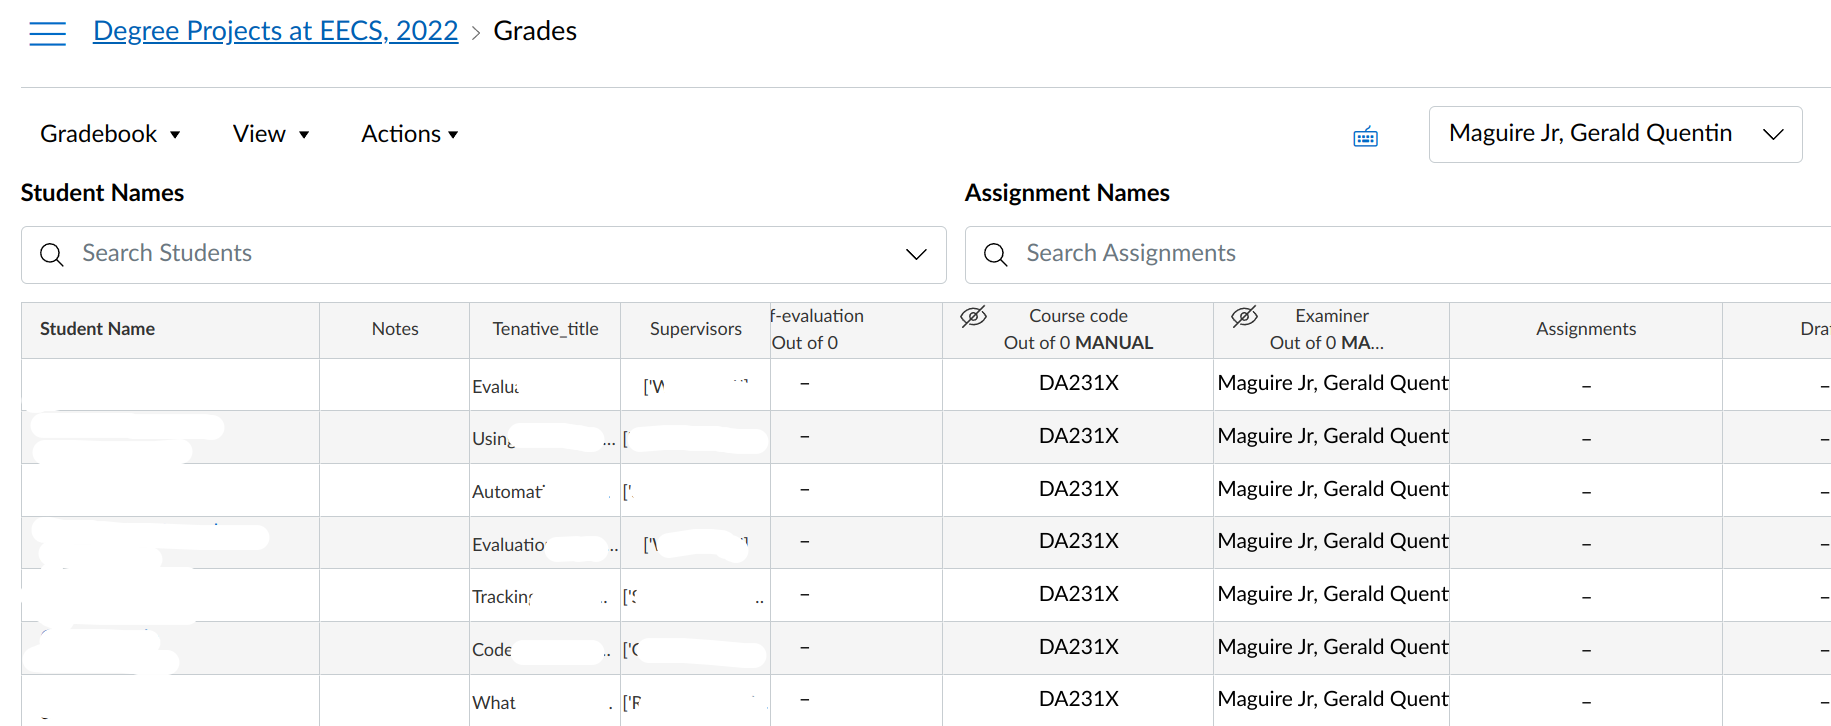
\includegraphics[width=0.99\textwidth]{README_notes/README-examiner-figures/part-of-my-students-Screenshot_20220325_152422-edited.png}
  \end{center}
  \caption{Examiner's view of the gradebook)}
  \label{fig:examinersViewOfGradebook}
\end{figure}

Note that in \Cref{fig:examinersViewOfGradebook}, there are two columns “Course code” and “Examiner”. These are what I call \textit{administrative assignments} and the students do not need to see them (hence the eye symbol with a slash through it – indicating these are hidden from the students). In the “Course code” assignment, I have given the student a “grade” that is the course code of their degree project. This way it is very easy to see what course code a student is enrolled in – as an examiner or supervisor may have students enrolled in several different course codes. This “grading standard”\footnote{What Canvas calls a grading standard is often called a grading scale.} was created from the list of all the EECS second-cycle course codes that share this same Canvas course room. The “Examiner” column contains a “grade” that is the name of the examiner assigned for this student. The examiner “grading standard” is created from the list of all of the examiners in the Canvas course room. In the same way that a teacher can assign a grade, if you click on the gradebook cell for a student, you get a pull-down list of all of the possible “grades” in this case the list of examiners, see \Cref{fig:listOfExaminers}.
\begin{figure}[!ht]
  \begin{center}
    
\includegraphics[width=0.5\textwidth]{README_notes/README-examiner-figures/top-of-the-list-of-examiners-Screenshot_20220325_153634.png}
  \end{center}
  \caption[List of examiners]{List of examiners (with the names erased to avoid GDPR problems)}
  \label{fig:listOfExaminers}
\end{figure}

Did I have to manually enter all of the course codes for the 687 students in the course room? No, I used a script via the command shown in \Cref{lst:addCourseCodesForStudentsInCourse}.  This required that initially the grading standard with course codes be created. It was created with the command shown in \Cref{lst:insertCourseCodeGradingStandard}.
\Needspace*{3\baselineskip}
\begin{lstlisting}[language={bash}, caption={add\_course\_codes\_for\_students\_in\_course.py}, label=lst:addCourseCodesForStudentsInCourse]
./add_course_codes_for_students_in_course.py 33514
\end{lstlisting}
\Needspace*{3\baselineskip}
\begin{lstlisting}[language={bash}, caption={insert\_course\_code\_grading\_standard.py}, label=lst:insertCourseCodeGradingStandard]
./insert_course_code_grading_standard.py 33514
\end{lstlisting}
\Needspace*{3\baselineskip}
The grading standard for examiners (and even one for teachers as supervisors) is created with the command shown in  \Cref{lst:insertTeachersGradingStandard}. To create the teachers grading standard you leave off the ``--emaniners'' option.

%% the following conditional is needed to avoid problems with "--" in the listing when using pdflatex
\ifxeorlua
\begin{lstlisting}[language={bash}, caption={insert\_teachers\_grading\_standard.py}, label=lst:insertTeachersGradingStandard]
./insert_teachers_grading_standard.py –-examiners 33514
\end{lstlisting}
\else
\begin{lstlisting}[%language={bash}, 
  basicstyle=\ttfamily, extendedchars=false,
caption={insert\_teachers\_grading\_standard.py}, label=lst:insertTeachersGradingStandard]
./insert_teachers_grading_standard.py –-examiners 33514
\end{lstlisting}
\fi

The command line shown in \Cref{lst:insertTeachersGradingStandard} creates a grading standard with the suffix “\_Examiners”. Note that all of these grading standards are \textit{course specific} grading standards, so they are invisible outside of this course room. One caution about the use of grading standards is that if the list of course codes or list of teachers/examiners changes – there can be problems with the mappings as the grading standard creates a mapping between a numeric grade and a string (the course code or name); therefore, they should only be generated once at the start of the course when the full list of values is known.

So clearly we can have information about the student, supervisors (who are teachers in the course), and examiner in the Canvas course room. Then since these people are in the Canvas course room we can know their sort-able name, KTHID, e-mail address, etc. Clearly, the students were added to the course when they were enrolled in the course. How did the teachers and examiners get into the course? These people were added to the course by a script that IT runs that takes this data from Kurs- och programplaneringssystemet (KOPPS)!

\subsection{How can we associate students with examiners and supervisors?}
In the case of the computer science (CS) students, the exjobb coordinator XXXXX\footnote{The person's name has been removed, to avoid issues with GDPR.} has a spreadsheet with the student’s name, working title, examiner, and supervisors in it. It has a sheet named “Closed” that contains information about the students who have been assigned an examiner and supervisor. \Cref{fig:spreadsheetOfCSStudents} shows the column headings of the spreadsheet “Masters\_thesis\_proposals-CS-P3-2022a.xlx” (this is my local file name for the spreadsheet).
	
\begin{figure}[!ht]
  \begin{center}
    
\includegraphics[width=0.99\textwidth]{README_notes/README-examiner-figures/sheet-columns-Screenshot_20220325_155622.png}
  \end{center}
  \caption{Columns in the `Closed' sheet of spreadsheet of CS students)}
  \label{fig:spreadsheetOfCSStudents}
\end{figure}

\Needspace*{6\baselineskip}
A script takes the data from this spreadsheet and adds the information to the Canvas gradebook with the command shown in \Cref{lst:insertExaminersAndSupervisorsFromSpreadsheet}.
\begin{lstlisting}[language={bash}, caption={insert-examiners-and-supervisors-from-spreadsheet.py}, label=lst:insertExaminersAndSupervisorsFromSpreadsheet]
./insert-examiners-and-supervisors-from-spreadsheet.py  33514   "Masters_thesis_proposals-CS-P3-2022a.xlsx"  
\end{lstlisting}
The script uses the student’s e-mail address to look up the student in the Canvas course room, then adds the student to the examiner’s section and updates the “Examiner” grade for this student to show this assigned examiner. It also adds the contents of “Proposal” field from the spreadsheet as text in a custom column in the gradebook called “Tentative\_title” and adds the list of supervisors to the custom column called “Supervisors” – see \Cref{fig:examinersViewOfGradebook}. Note that this program uses a JavaScript Object Notation (JSON) file, \texttt{spreadsheet\_aliases-33514.json}, containing aliases for each of the examiners and supervisors. \Cref{lst:aliasFile} shows part of the alias file.
\Needspace*{15\baselineskip}	
\begin{lstlisting}[language={Python}, caption={Some of the contents of an alias file for a course}, label=lst:aliasFile]
{
    "examiners": {
        "Anders Västberg": "Västberg, Anders",

        "Gerald Maguire": "Maguire Jr, Gerald Quentin",
        "Gerald  Q.  Maguire": "Maguire Jr, Gerald Quentin",

    },
    "teachers": {
    
    }
}
\end{lstlisting}

The alias file takes the names used in the spreadsheet (the name shown on the left in the listing above) and maps them to the sortable names used in Canvas (the name shown on the right in the listing above). While this adds a little more complexity, it addressed the problem that the names used in the spreadsheet are not always consistent or even complete.

The availability of information in Canvas also suggests that some of the arguments that were shown earlier for the script \texttt{create\_customized\_JSON\_file.py} are actually unnecessary and the program can figure them out given the course\_id and student’s e-mail address. However, some things are not accessible directly from Canvas, for example, I have not been able to figure out what exam a student intends to apply for following their degree project course. Another example of missing information is the program code; however, this information is in LADOK and Canvas has the LADOK identifier for each student; however, my script to access LADOK is currently not working.
\Needspace*{8\baselineskip}
\subsection[What happens if I do not have such a spreadsheet?]{What happens if I do not have such\\ a spreadsheet?}

A Canvas administrator can add students to the examiner’s and supervisor’s sections, as shown in \Cref{fig:sectionEntrollments}. Note that the input field can do partial matches on the text that you enter and will give you a list of the partially matching entries and then you can click on one and then click on Update. 
 	
\begin{figure}[!ht]
  \begin{center}
    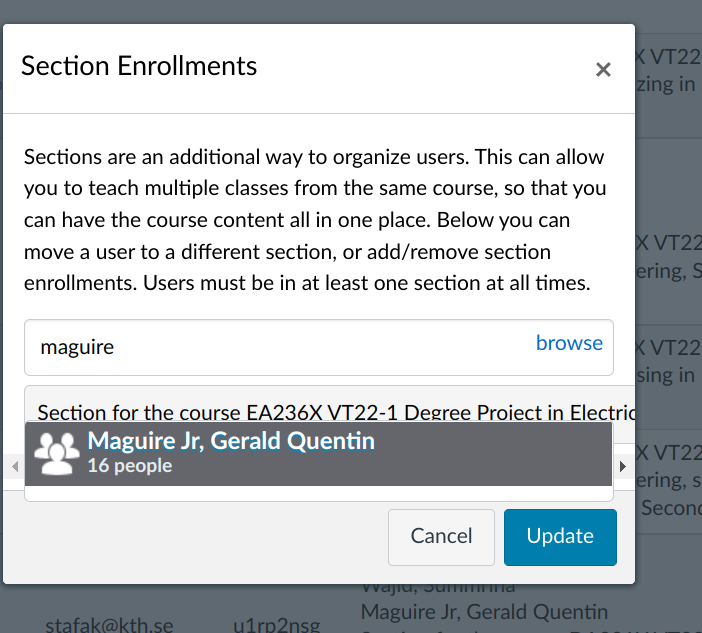
\includegraphics[width=0.99\textwidth]{README_notes/README-examiner-figures/edit-sections-Screenshot_20220325_161529.png}
  \end{center}
  \caption{Section enrollments)}
  \label{fig:sectionEntrollments}
\end{figure}
\FloatBarrier

To get the Section Enrollments editing box popup (shown above) – you go to the “People” page – find the student (either scrolling down the page or starting to type the student’s name in “Search people” box (shown in \Cref{fig:peopleSearchbox}) then click on the vertical three dots on the right side of the row for this student and click on Edit section (as shown in \cref{fig:editSectionsButton}).
\begin{figure}[!ht]
  \begin{center}
    
\includegraphics[width=0.5\textwidth]{README_notes/README-examiner-figures/Search-people-Screenshot_20220325_161811.png}
  \end{center}
  \caption{Search people box on People page}
  \label{fig:peopleSearchbox}
\end{figure}
	
\begin{figure}[!ht]
  \begin{center}
    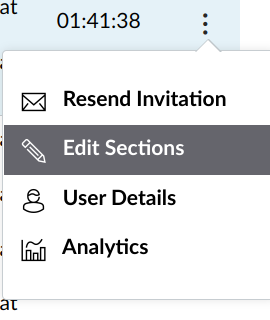
\includegraphics[width=0.5\textwidth]{README_notes/README-examiner-figures/edit-section-cmd-Screenshot_20220325_162252.png}
  \end{center}
  \caption{Three vertical dots and Edit Sections button}
  \label{fig:editSectionsButton}
\end{figure}
\FloatBarrier

Now that we have tied together the student, examiner, and supervisors; we can make use of that information in many ways. One of these ways was to create the customized \LaTeX\;project described earlier. The next section will explain some of the additional steps in the degree project that can be partially automated.
\Needspace*{12\baselineskip}
\section{Automating later steps in the degree project}
\label{sec:AutomatingLaterSteps}
There are many different steps in the degree project that can be facilitated by using the information from the Canvas course room and from the student's thesis. An example of one of these is making an announcement for the student's oral presentation (described in \Cref{sec:makingAnAnnouncement}). Another example is facilitating entering the metadata about the thesis into DiVA (see \Cref{sec:facilitatingDiVAentry}).

\subsection{Making an announcement}
\label{sec:makingAnAnnouncement}
When the examiner has set a time, place, \ldots for the student's oral presentation, then assuming that a student has submitted their thesis with the information in the “For DIVA” pages and that this information includes the information about the opponent(s) and presentation (\eg time, place, zoom link), the steps to make an announcement are:
\begin{enumerate}
    \item Save the PDF file of the thesis, for example \texttt{oscar.pdf}
    \item Extract the “For DIVA” information as JSON, as shown in \Cref{lst:extractPseudoJSONFromPDFforOscarFileToJSON}\footnote{For information about an alternative way to get the JSON file, see \Cref{sec:optimizeJSONToMods}.}
    
    If acronyms are used in the abstracts, you can add the “--acronyms acronyms.tex” argument to the extract command line and the program will process the acronyms from the acronyms.tex file (this means that you will also need this file). The output of the program is a JSON file (oscar.json) that can subsequently be used to make an announcement.
    
    \item Make the announcement for a Canvas course room (in this case, for a Canvas course room with course\_id 11), as shown in \Cref{lst:jsonToCalenarforOscar1}.
    
    Replace 11 with the course\_id of the Canvas course room, for example, 33514 for the EECS second-cycle degree projects during 2022.
\end{enumerate}
\Needspace*{7\baselineskip}
\begin{lstlisting}[language={bash}, caption={extract\_pseudo\_JSON-from\_PDF.py for Oscar}, label=lst:extractPseudoJSONFromPDFforOscarFileToJSON]    
   ./extract_pseudo_JSON-from_PDF.py --pdf oscar.pdf --json oscar.json
\end{lstlisting}

\begin{lstlisting}[language={bash}, caption={JSON\_to\_calendar.py for Oscar}, label=lst:jsonToCalenarforOscar1] 
./JSON_to_calendar.py -c 11 --json oscar.json
\end{lstlisting}
The command line shown in \Cref{lst:jsonToCalenarforOscar1} will publish the announcement in \first Canvas course 11, \Second in the Canvas course’s calendar, and \third (eventually) in the KTH Calendar. To publish a KTH calendar event, the software supports the development version of the KTH Cortina API. However, this is API not yet in production and requires a KTH Cortina Access Key.

 For more information see Sections~\ref{sec:whatCanweDoWithTheJSONfile} and \ref{sec:otherVariantsofJSONtoCalendar}.

\subsection{Making a cover and applying it}
\label{sec:makingACover}
As of December 2021, there is a new cover for 1\textsuperscript{st} and second-cycle theses at KTH. Information about this is at \url{https://intra.kth.se/en/administration/kommunikation/mallar/avhandlingarochexamensarbeten/skapa-ett-omslag-till-ditt-exjobb-1.479838}.

When the student is writing their thesis, they can set up the title and subtitle in English and Swedish by simply editing the relevant lines in the \LaTeX~file, see \Cref{lst:titleSubtitleEtc}. This is further described in detail in \Cref{sec:putInformationIntoLatexTemplate}  
\iflabelexists{ch:READMEnotes}{and \Cref{ch:READMEnotes}}
{- You have to include the \texttt{README\_notes/README\_notes.tex} file when compiling to get additional information.}

\Needspace*{12\baselineskip}
\begin{lstlisting}[language={[LaTeX]TeX}, caption={Title and subtitle in the two languages}, label=lst:titleSubtitleEtc] 
\title{This is the title in the language of the thesis}
\subtitle{A subtitle in the language of the thesis}

% give the alternative title - i.e., if the thesis is in English, then give a Swedish title
\alttitle{Detta är den svenska översättningen av titeln}
\altsubtitle{Detta är den svenska översättningen av undertiteln}
% alternative, if the thesis is in Swedish, then give an English title
%\alttitle{This is the English translation of the title}
%\altsubtitle{This is the English translation of the subtitle}
  \end{verbatim}
  \caption{Title, subtitle, etc.)}
  \label{fig:titleSubtitleEtc}
\end{lstlisting}

In the case of the \LaTeX\;project, the cover is automatically made and updated as the student writes their thesis. The only things that are needed for the cover that are missing is the exam that the student is going to take out and the TRITA number. We will assume that the student has entered the exam that they are going to apply for in their \LaTeX~file.

Within School of XXX\footnote{Name replaced to neutralize the template.}, the Office of Student Affairs assigns the TRITA number when the examiner has approved the thesis and submitted the PDF file of the approved thesis\footnote{This PDF file is supposed to have the front and back covers; however, as can be seen from the temporal ordering there is a problem as the back cover is made and applied \textbf{before} the number is assigned. One possible solution for this would be to not apply the back cover, but rather have the back cover created and applied by the Office of Student Affairs after they have assigned the TRITA number. Another possible solution would be to tell the examiner the TRITA number so that it can be added to the project and the cover and MODS file made. I think that ideally the TRITA number should be assigned by a program (and stored in a database) and the same program can make and add to the PDF of the thesis. Additionally, the assignments of TRITA numbers in the database can be sent to the archiving unit each year.}. The TRITA number needs to be \first added to the project before generating the final PDF file or \Second alternatively it can be entered by editing the placeholder text on the back cover when the TRITA number is assigned. Note that in the latter case, this data has to be (a) added to the JSON file used to make the MODS file (see \Cref{sec:facilitatingDiVAentry}) or (b) manually edited in DiVA entry.

So what we have seen (in this and other sections) is that we can use the information from Canvas and the thesis itself for simplifying many steps of the degree project process. For example, by having the thesis itself have both the English and Swedish titles and subtitles, it should be easier to add this information to both DiVA and LADOK. The underlying assumption is that the correct and relevant data will be in the Canvas course room and in the thesis itself!
\clearpage

\subsection{To facilitate entering a thesis into DiVA – make a MODS file}
\label{sec:facilitatingDiVAentry}
Assuming that a student has submitted a thesis with the information in the “For DIVA pages” that includes the information for the DIVA entry and the examiner has approved the thesis.

The same steps as described in \Cref{sec:makingACover} are made to save the PDF file and extract the “For DIVA” information as JSON\footnote{For information about an alternative way to get the JSON file, see \Cref{sec:optimizeJSONToMods}.}. This JSON file is then used to make a MODS file via the command shown in \Cref{lst:jsonToMODSforOscar}. Note that in this case, we assume that the person running the program knows the TRITA number; otherwise, the value of the TRITA number in the JSON file is used.
\Needspace*{4\baselineskip}
\begin{lstlisting}[language={bash}, caption={JSON\_to\_MODS.py for Oscar}, label=lst:jsonToMODSforOscar] 
./JSON\_to\_MODS.py -c 11   --json oscar.json --trita "TRITA-XXX-EX-2021:xxxx"
\end{lstlisting}

One way of getting the JSON information to make the MODS file is given in \Cref{sec:optimizeJSONToMods}. A description of how the JSON is converted to a MODS file is given in \Cref{sec:JSONtoMODSfile}.

\section{Can someone else use these programs?}
The source code is at \url{https://github.com/gqmaguirejr/E-learning}. Get the programs from the github, then create a config.json file to provide your Canvas access token and the URL of the Canvas instance you want to use, for details see \url{https://canvas.kth.se/courses/11/pages/making-a-config-dot-json-file-to-make-life-simpler} 

To run the program to make announcements and calendar entries for a course room requires the program and appropriate permissions  to post announcements in a course and insert course calendar events (for example, if the user is a Teacher in the specific Canvas course room or as a Canvas administrator). To make the entry in the KTH Calendar requires a KTH Cortina access key. Making the MODS file does not require any specific permissions as the program is run locally.

To change sections (adding/removing/\ldots a user to/from a section) requires the permissions of a Canvas administrator. However, this is something that E-learning should change about the KTH Canvas configuration; as this should be something that the examiner(s) or course-responsible persons should be able to do. Additionally, the KTH Cortina Calendar API requires an access key (which you have to get from the IT unit).

\Needspace*{12\baselineskip}
\section{\LaTeX~template in Overleaf}
A \LaTeX~template in Overleaf is at \url{https://www.overleaf.com/read/qxvttmmqbgdt} - this is the version used by many students.

Details about using the template are in  
\iflabelexists{ch:READMEnotes}{\Cref{ch:READMEnotes}.}
{xxxx - You have to include the \texttt{README\_notes/README\_notes.tex} file when compiling to get additional information.}
Note that the rest of this document goes into deep detail about \textit{how} the \textbf{template} works and \textit{how} the \textbf{programs} work. The primary intention is to give the information necessary so that someone else can take over the template and programs. Also note that \Cref{sec:accessibility} addresses issues about accessibility.
 
\section{Put information into \LaTeX~template to generate a draft or final thesis}
\label{sec:putInformationIntoLatexTemplate}

\Cref{fig:sampleTitlePage} shows the title page of a fictitious thesis created using a \LaTeX~template that I have developed. The idea is to capture in the thesis itself all of the information needed for this title page, the cover pages, the announcement of the oral presentation, and for reporting the final approved thesis in DiVA via the thesis itself.

\begin{figure}[!ht]
  \begin{center}
    \fbox{
\includegraphics[width=0.85\textwidth]{README_notes/README-examiner-figures/Title-page-20220329.pdf}}
  \end{center}
  \caption{Example of a title page}
  \label{fig:sampleTitlePage}
\end{figure}
\clearpage

For the current documentation of the template for these details, please see the file “README\_notes.tex” in the template itself - 
\iflabelexists{ch:READMEnotes}{\Cref{ch:READMEnotes}.}
{You have to include the \texttt{README\_notes/README\_notes.tex} file when compiling to get additional information.}
What follows includes some older examples – so there may be differences in the details between these examples and the current template.

For the purpose of this document, the following information is present in the order of this exposition, not necessarily the order it is in the \LaTeX~source file. However, all of this information is prior to \textbackslash begin{document}. In particular, information that should be knowable at the start of the degree project is placed into a file named \texttt{custom\_configuration.tex} – to make it easier to pre-configure a project for a student or students (as was described in \Cref{sec:makeItSimpleFromTheStart}).

Information about the title and the student author(s) of the thesis is entered via the set of commands as shown in Listings~\ref{lst:titles} and \ref{lst:authors}. Note that you can have either one or two authors (the latter should generally only occur in the case of a first-cycle degree project). There are several other elements of metadata collected about the student (primarily driven by the current author metadata fields in DiVA). A brief description of them and why they are there are given below:
\begin{itemize}
    \item One might question why have an e-mail address (when under the current policy is that the student will lose their e-mail address upon graduation)? One of the main reasons is so that the library (\ie KTHB) can notify the student that the thesis has be stored in DiVA. A second reason is if the library needs to contact the student.
    
    \item One might also wonder, why include the student’s \texttt{kthid} (\ie their internal to KTH ID). The main reason is that this identifier \textit{uniquely identifies} this author within KTH, so that all of their publications can be found in a DiVA search. Note that a number of KTH students go on to write papers related to their thesis and a number of these are registered in DiVA. Without a unique identifier, it would not be possible to connect these different documents.
    
    \item A very questionable field is \texttt{authorsSchool}. In a discussion with DiVA administrators at KTH on 2021-04-29, the consensus was that this should be the school of the thesis examiner, since 1\textsuperscript{st} and second-cycle students are in \textbf{programs of study} and not schools, department, \etc.
    
    \item Next there is \texttt{programcode} – this is used to generate the degree information just above the other data on the title page and is also used to compute the “lead” for the calendar entry (which differs depending upon whether it is a 1\textsuperscript{st} or second-cycle degree project presentation).
    
    \item Finally, the \texttt{degreeName} and \texttt{subjectArea}, \eg \textbackslash degreeName{Bachelors degree} \textbackslash subjectArea{Technology }- provide information that is used later when generating the color KTH cover.
\end{itemize}
\textbf{NB}: A limitation of the current template is that I do not handle the case of two students who are in different programs.

The template previously supported ORCID IDs for students, but as per email from KTH Biblioteket on 2021-06-28, students cannot have an OrCiD reported for their degree project; therefore, this functionality was removed.


An example of information about the title and student authors for a thesis is shown in Listings~\ref{lst:titles} and \ref{lst:authors} (respectively).
\Needspace*{12\baselineskip}
\begin{lstlisting}[language={[LaTeX]TeX}, caption={Information about the titles and subtitles of the thesis}, label=lst:titles]
\title{This is the title in the language of the thesis}
\subtitle{A subtitle in the language of the thesis}

% give the alternative title - i.e., if the thesis is in English, then give a Swedish title
\alttitle{Detta är den svenska översättningen av titeln}
\altsubtitle{Detta är den svenska översättningen av undertiteln}
% alternative, if the thesis is in Swedish, then give an English title
%\alttitle{This is the English translation of the title}
%\altsubtitle{This is the English translation of the subtitle}
\end{lstlisting}
\Needspace*{32\baselineskip}
\begin{lstlisting}[language={[LaTeX]TeX}, caption={Information about the student authors of the thesis}, label=lst:authors] 
\authorsLastname{Student}
\authorsFirstname{Fake A.}
\email{a@kth.se}
\kthid{u100001}
\authorsSchool{\schoolAcronym{XXX}}
%If the student is not in Stockholm, Sweden, add that information here
% This information will be used when generating the acknowledgements signature.
%\authorCity{A City}
%\authorCountry{A Country}
% pass into \authorCityCountryDate{} the month and year for the acknowledgment
% If there is a second author and place, the month, and year are the same, the specify the month and year for the first author:
\authorCityCountryDate{\MONTH\enspace\the\year}
% if there is a second author and the place is different, then say:
%\authorCityCountryDate{}

% If there is a second author - add them here:
\secondAuthorsLastname{Student}
\secondAuthorsFirstname{Fake B.}
\secondemail{b@kth.se}
\secondkthid{u100002}
\secondAuthorsSchool{\schoolAcronym{XXX}}
%If the student is not in Stockholm, Sweden, add that information here
% This information will be used when generating the acknowledgements signature.
%\secondAuthorCity{A City}
%\secondAuthorCountry{A Country}
% pass into \secondAuthorCityCountryDate{} the month and year for the acknowledgement
%\secondAuthorCityCountryDate{\MONTH\enspace\the\year}
%\secondAuthorCityCountryDate{}
\end{lstlisting}


\Cref{lst:hostcompany} shows how to enter data about where the thesis is being done if outside of KTH.
\textbf{NB}: A limitation of the current template is that I do not handle multiple companies, as I assume that there is a single host company. However, you can have a list of names within the two text fields (but only a single \textbackslash hostcompany or a single \textbackslash hostorganization should be included). As of the DiVA administrators meeting of 2022-03-25, if there are a list of names, they should be separated by a semicolon or vertical bar (\ie the `|' character) and the information should be entered in an uniform manner (\ie ``på ett enhetligt sätt''). However, there is not yet a list of the partner names in canonical form. Moreover, it was also noted that if the name of the company or organization is confidential, then the field should contain the string ``Confidential'' and when the DiVA entry is made the actual name or the company or organization should be entered in the ``Internal'' information field (\ie ``intern kommentar'') in DiVA. Unfortunately, it is not clear how the DiVA administrator would know this information. However, 
the KTHB bibliometrics unit is interested in this data, as is the GVS unit working with industrial relations.
\Needspace*{5\baselineskip}
\begin{lstlisting}[language={[LaTeX]TeX}, caption={Information about where the thesis is taking place}, label=lst:hostcompany] 
\hostcompany{Företaget AB} % Remove this line if the project was not done at a host company
%\hostorganization{CERN}   % if there was a host organization
\date{\today}
\end{lstlisting}
\Needspace*{17\baselineskip}
\Cref{lst:oralpresentatioOpponents} collects the information regarding the time, place, and language of the presentation. Note that the opponents' names are simply separated by ‘\&’ – so it is easy to have one more opponent.
\ifxeorlua
\begin{lstlisting}[language={[LaTeX]TeX}, caption={Information relevant to the oral presentation (both the location and the opponent or opponents)}, label=lst:oralpresentatioOpponents] 
%%%%% For the oral presentation
%% Add this information once your examiner has scheduled your oral presentation
\presentationDateAndTimeISO{2022-03-15 13:00}
\presentationLanguage{eng}
\presentationRoom{via Zoom https://kth-se.zoom.us/j/ddddddddddd}
\presentationAddress{Isafjordsgatan 22 (Kistagången 16)}
\presentationCity{Stockholm}

% Opponent's information
\opponentsNames{A. B. Normal \& A. X. E. Normalè}

\nationalsubjectcategories{10201, 10206}
\end{lstlisting}
\else
\begin{lstlisting}[language={[LaTeX]TeX}, extendedchars=false, caption={Information relevant to the oral presentation (both the location and the opponent or opponents)}, label=lst:oralpresentatioOpponents] 
%%%%% For the oral presentation
%% Add this information once your examiner has scheduled your oral presentation
\presentationDateAndTimeISO{2022-03-15 13:00}
\presentationLanguage{eng}
\presentationRoom{via Zoom https://kth-se.zoom.us/j/ddddddddddd}
\presentationAddress{Isafjordsgatan 22 (Kistagången 16)}
\presentationCity{Stockholm}

% Opponent's information
\opponentsNames{A. B. Normal \& A. X. E. Normalè}

\nationalsubjectcategories{10201, 10206}
\end{lstlisting}
\fi
\Needspace*{12\baselineskip}
Finally, \Cref{lst:nationalSubjects} collects the information regarding the National Subject Categories – this is simply a list of 3 or 5 digit numbers separated by commas. The numbers come from \url{https://www.scb.se/contentassets/10054f2ef27c437884e8cde0d38b9cc4/oversattningsnyckel-forskningsamnen.pdf} while the Swedish and English versions are given in \url{https://www.scb.se/contentassets/3a12f556522d4bdc887c4838a37c7ec7/standard-for-svensk-indelning--av-forskningsamnen-2011-uppdaterad-aug-2016.pdf}. This information is for a required field in DiVA. Note that 5 digit codes are preferred over 3 digit codes.
\begin{lstlisting}[language={[LaTeX]TeX}, caption={Information relevant to the oral presentation (both the location and the opponent or opponents}, label=lst:nationalSubjects] 
\nationalsubjectcategories{10201, 10206}
\end{lstlisting}

The program \texttt{create\_customized\_JSON\_file.py} tries to guess the National Subject Categories based upon the particular course code that the student is enrolled in. Currently only the categories that I thought were useful for the EECS second-cycle courses codes are well addressed.

\Cref{lst:EnglishAbstractLang} and \Cref{lst:EnglishAbstract} show examples of abstracts that in a real thesis would be in English and Swedish with the first to appear being the abstract in the language of the thesis. Note that the actual content of these two abstracts is primarily for testing and is not meant to suggest real abstracts. However, these examples show some of the equations and symbols that are supported (\ie in the Canvas announcement, calendar postings, and in DiVA).

The template also supports a number of other languages (based on the languages used for abstracts in undergraduate theses in 2020). It is straightforward to add an additional language as necessary. One of the reasons for having abstracts in additional languages is so that dual degree students do not have to write another document for their home/other university. While the template includes a number of placeholders for these other abstracts, if they are unused they can simply be deleted.
The three-character code used for the language is the ISO 639-2 Code – specifically, the "B" (bibliographic) variant of these codes --- as these seem to be the codes used in DiVA when one accesses the MODS formatted metadata for publications. In the example below we see “eng” being stored into a scontents buffer called “lang”.
\Needspace*{5\baselineskip}
\begin{lstlisting}[language={[LaTeX]TeX}, caption={Storing the language in a scontents buffer named "lang"}, label=lst:EnglishAbstractLang] 
\begin{scontents}[store-env=lang]
eng
\end{scontents}
\end{lstlisting}

The abstract itself is stored in an scontents buffer called “abstracts” and the keywords are stored in an scontents buffer called “keywords”.  These buffers are part of the \LaTeX~\texttt{scontents} package and allow contents to be stored and later retrieved. Note that an internal function is used inside this package, so that the abstracts can be stored in raw \LaTeX~code - rather than being stored after being processed. This was done to retain the \LaTeX~codes for mathematics and symbols - so they can be processed into the necessary forms for where they are to be used (\ie in the Canvas announcement, calendar postings, and in DiVA). Further details of the magic of scontents buufers are given in \Cref{sec:scontentsHack}.

\textbf{NB}: Because the raw \LaTeX~code is stored the acronyms need to be processed later by a program (this is described later) - it is suggested that the acronyms be spelled out in the non-English language abstracts, as I do not know how to support them - as multiple language glossaries is not something that I understand how to do nor do I know how to properly generate plurals of Swedish acronyms.

\textbf{NB}: It is assumed that no abstracts or keywords include \textbf{four euro symbols in a row} (\ie quad euro symbols) - as these are used as markers in the file to mark the boundaries of abstracts and lists of keywords.
\Needspace*{34\baselineskip}
\begin{lstlisting}[language={[LaTeX]TeX}, caption={Storing the language in a scontents buffer named "lang"}, label=lst:EnglishAbstract]
\begin{abstract}
  \markboth{\abstractname}{}
\begin{scontents}[store-env=lang]
eng
\end{scontents}
\begin{scontents}[store-env=abstracts,print-env=true]
All theses at KTH are \textbf{required} to have an abstract in both \textit{English} and \textit{Swedish}.

Exchange students may want to include one or more abstracts in the language(s) used in their home institutions to avoid the need to write another thesis when returning to their home institution.

Keep in mind that most of your potential readers are only going to read your \texttt{title} and \texttt{}abstract}. This is why it is important that the abstract give them enough information that they can decide if this document relevant to them or not. Otherwise, the likely default choice is to ignore the rest of your document.

An abstract should stand on its own, i.e., no citations, cross-references to the body of the document, acronyms must be spelled out, … .

Write this early and revise as necessary. This will help keep you focused on what you are trying to do.

Example of a formula in an abstract: $c=2 \cdot \pi \cdot r$ or \[ \int_{a}^{b} x^2 \,dx \]
two chemical formulas: H\textsubscript{2}O or $(C_5O_2H_8)_n$, copyright symbol: \textcopyright Maguire 2021, and some superscripts: \textsuperscript{99m}Tc, A\textsuperscript{*},
A\textsuperscript{\textregistered}, and A\texttrademark.

Write an abstract with the following components:% key parts of the abstract
\begin{itemize}
  \item …

\end{itemize}
% comment at end
\end{scontents}

\subsection*{Keywords}
\begin{scontents}[store-env=keywords,print-env=true]
Canvas Learning Management System, Docker containers, performance tuning
\end{scontents}
\end{abstract}
\end{lstlisting}



\Needspace*{40\baselineskip}
\begin{lstlisting}[language={[LaTeX]TeX}, caption={\LaTeX~input to produce the Swedish abstract}, label=lst:SwedishAbstract] 
 \selectlanguage{swedish} 
\begin{abstract}
    \markboth{\abstractname}{}
\begin{scontents}[store-env=lang]
swe
\end{scontents}
\begin{scontents}[store-env=abstracts,print-env=true]
Alla avhandlingar vid KTH måste ha ett abstrakt på både engelska och svenska.


If you are writing your thesis in English, you can leave this until the final version. If you are writing your thesis in Swedish, then this should be done first – and you should revise as necessary along the way.

If you are writing your thesis in English, this section can be a summary targeted at a more general reader. However, if you are writing your thesis in Swedish, then the reverse is true – your abstract should be for your target audience. Similarly, an English summary can be written targeted at a more general audience.

This means that the English abstract and Swedish sammnfattning  
or Swedish abstract and English summary need not be literal translations of each other.

The abstract in the language used for the thesis should be the first abstract, while the Summary/Sammanfattning in the other language can follow.
\end{scontents}
\subsection*{Nyckelord}
\begin{scontents}[store-env=keywords,print-env=true]
Canvas Lärplattform,Dockerbehållare, prestandajustering
\end{scontents}
\end{abstract}
\end{lstlisting}


\clearpage
\section{Now that data is in the template, what happens?}
\label{sec:nowThatDataIsInTheTemplate}

The first thing that happens is the \LaTeX~code automatically generates one or more pages at the end of the PDF document that contain the data – primarily to be used to report the final approved thesis in DiVA. However, a secondary use is that if this information is added to the draft copy that is going to the opponent – then one can potentially automate many of the steps in announcing the oral presentation (as was described in \Cref{sec:makingAnAnnouncement}).
\Needspace*{8\baselineskip}
Figures~\ref{fig:sampleFOrDIVApage1}, \ref{fig:sampleFOrDIVApage2}, and \ref{fig:sampleFOrDIVApage3} show this “For DIVA” information. The first page is shown as text in \Cref{lst:forDIVApg11Text}. The format is supposed to look like JSON.
For example, the text for the examiner's organization:
\begin{lstlisting}[language=json]
{"organisation": {"L1": "School of XXX",
                 "L2": "DepartmentName" }}}
\end{lstlisting}

\noindent is used to determine which local part of the KTH calendar a calendar announcement should appear in, as the Cortina calendar is divided by the school and then by department. Note that the department name must be in Swedish for Cortina.
\clearpage
\begin{figure}[!ht]
  \begin{center}
    \fbox{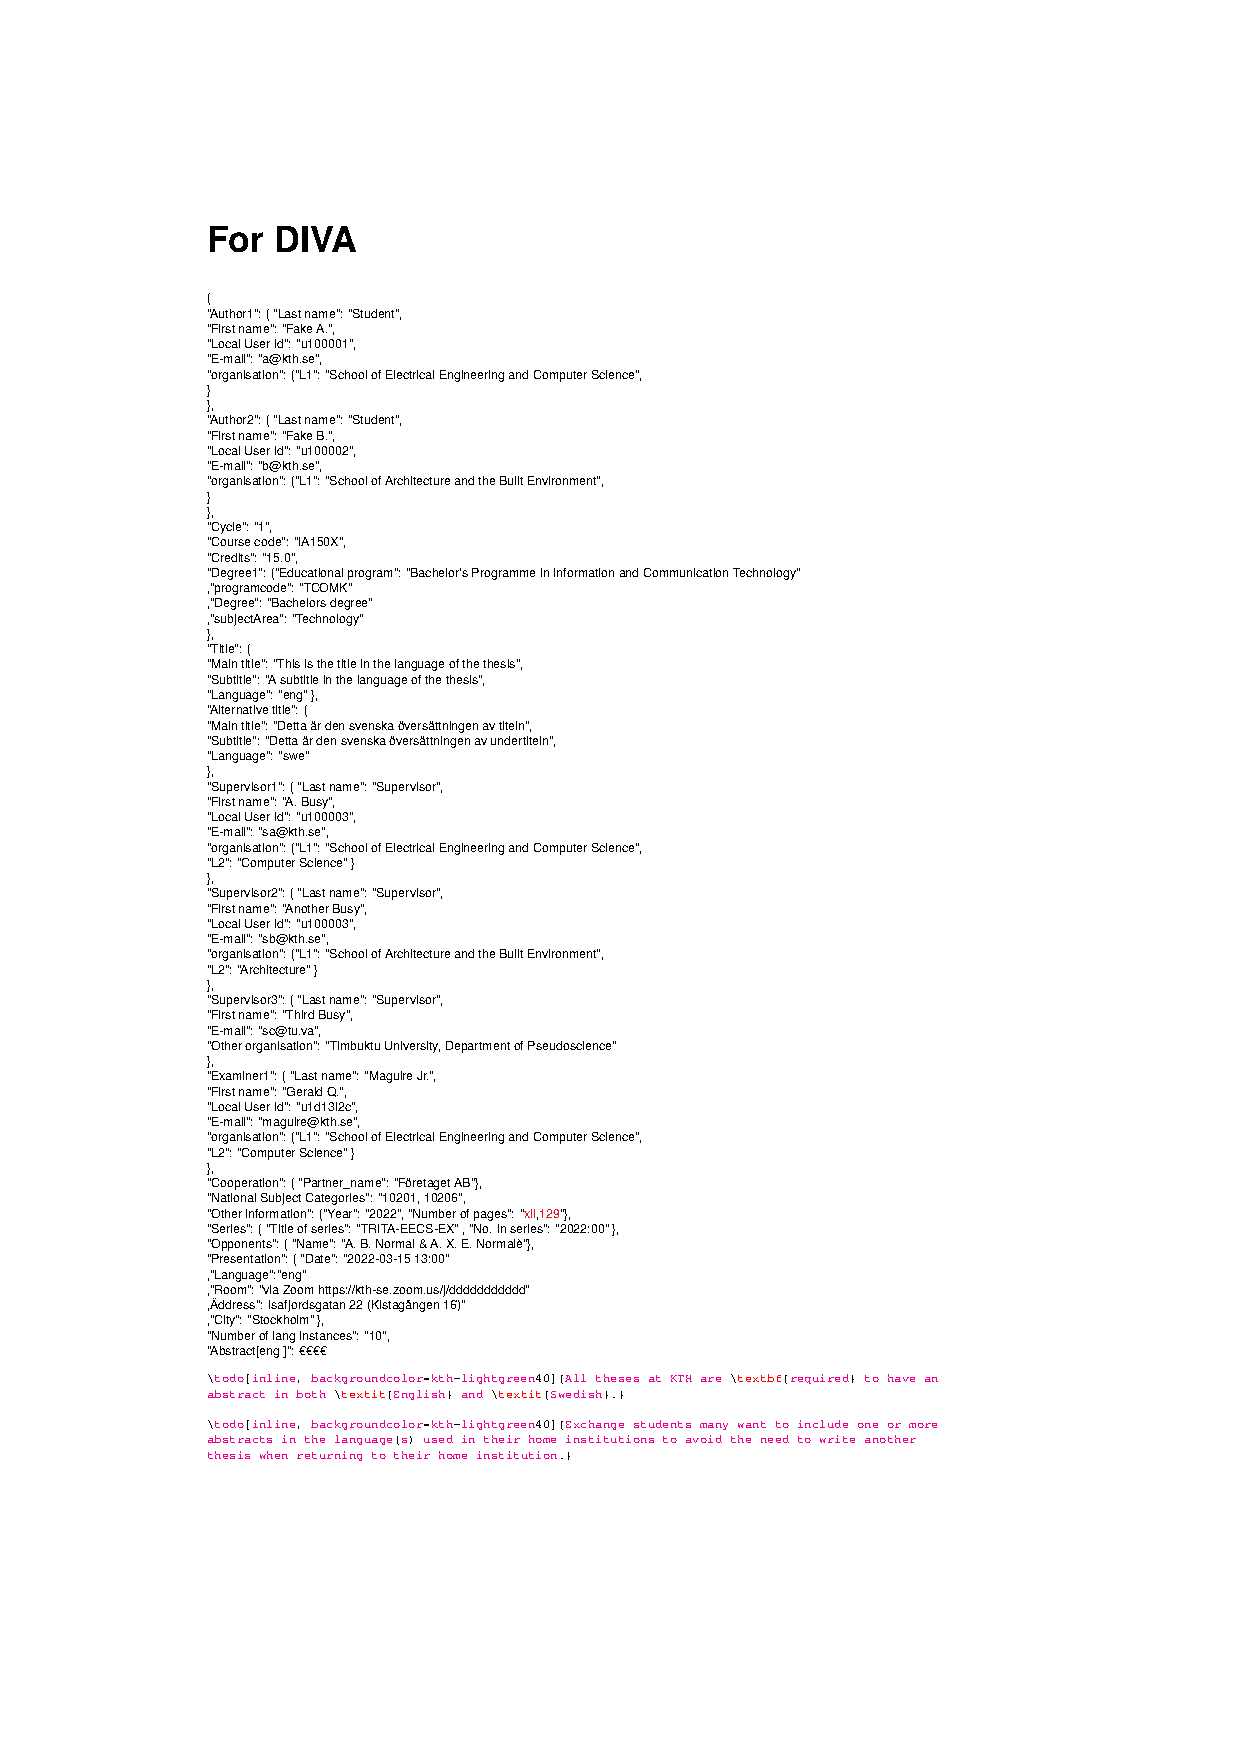
\includegraphics[width=0.85\textwidth]{README_notes/README-examiner-figures/ForDIVA-pg1.pdf}}
  \end{center}
  \caption{First page of the “For DiVA” information}
  \label{fig:sampleFOrDIVApage1}
\end{figure}
\clearpage
\begin{lstlisting}[language={json}, caption={Text version of the first page of the For DIVA output}, label=lst:forDIVApg11Text]
{
"Author1": { "Last name": "Student",
"First name": "Fake A.",
"Local User Id": "u100001",
"E-mail": "a@kth.se",
"organisation": {"L1": "School of XXX",
}
},
"Author2": { "Last name": "Student",
"First name": "Fake B.",
"Local User Id": "u100002",
"E-mail": "b@kth.se",
"organisation": {"L1": "School of XXX",
}
},
"Cycle": "1",
"Course code": "XX100X",
"Credits": "15.0",
"Degree1": {"Educational program": "Bachelor’s Programme in XXX"
,"programcode": "TCOMK"
,"Degree": "Bachelors degree"
,"subjectArea": "Technology"
},
"Title": {
"Main title": "This is the title in the language of the thesis",
"Subtitle": "A subtitle in the language of the thesis",
"Language": "eng" },
"Alternative title": {
"Main title": "Detta är den svenska översättningen av titeln",
"Subtitle": "Detta är den svenska översättningen av undertiteln",
"Language": "swe"
},
"Supervisor1": { "Last name": "Supervisor",
"First name": "A. Busy",
"Local User Id": "u100003",
"E-mail": "sa@kth.se",
"organisation": {"L1": "School of XXX",
"L2": "DepartmentName" }
},
"Supervisor2": { "Last name": "Supervisor",
"First name": "Another Busy",
"Local User Id": "u100003",
"E-mail": "sb@kth.se",
"organisation": {"L1": "School of XXX",
"L2": "DepartmentName" }
},
"Supervisor3": { "Last name": "Supervisor",
"First name": "Third Busy",
"E-mail": "sc@tu.va",
"Other organisation": "Timbuktu University, Department of Pseudoscience"
},
"Examiner1": { "Last name": "ExaaminersLastname",
"First name": "ExaaminersFistname",
"Local User Id": "u1000000",
"E-mail": "xxx@kth.se",
"organisation": {"L1": "School of XXX",
"L2": "DepartmentName" }
},
"Cooperation": { "Partner_name": "Företaget AB"},
"National Subject Categories": "ddddd, ddddd",
"Other information": {"Year": "2022", "Number of pages": "xli,133"},
"Series": { "Title of series": "TRITA-XXX-EX" , "No. in series": "2022:00" },
"Opponents": { "Name": "A. B. Normal & A. X. E. Normalè"},
"Presentation": { "Date": "2022-03-15 13:00"
,"Language":"eng"
,"Room": "via Zoom https://kth-se.zoom.us/j/ddddddddddd"
,"Äddress": Isafjordsgatan 22 (Kistagången 16)"
,"City": "Stockholm" },
"Number of lang instances": "10",
"Abstract[eng ]": €€€€
\engExpl{All theses at KTH are \textbf{required} to have an
abstract in both \textit{English} and \textit{Swedish}.}
\engExpl{Exchange students many want to include one or more
abstracts in the language(s) used in their home institutions to avoid the need to write another
thesis when returning to their home institution.}
\end{lstlisting}
\clearpage
\begin{figure}[!ht]
  \begin{center}
    \fbox{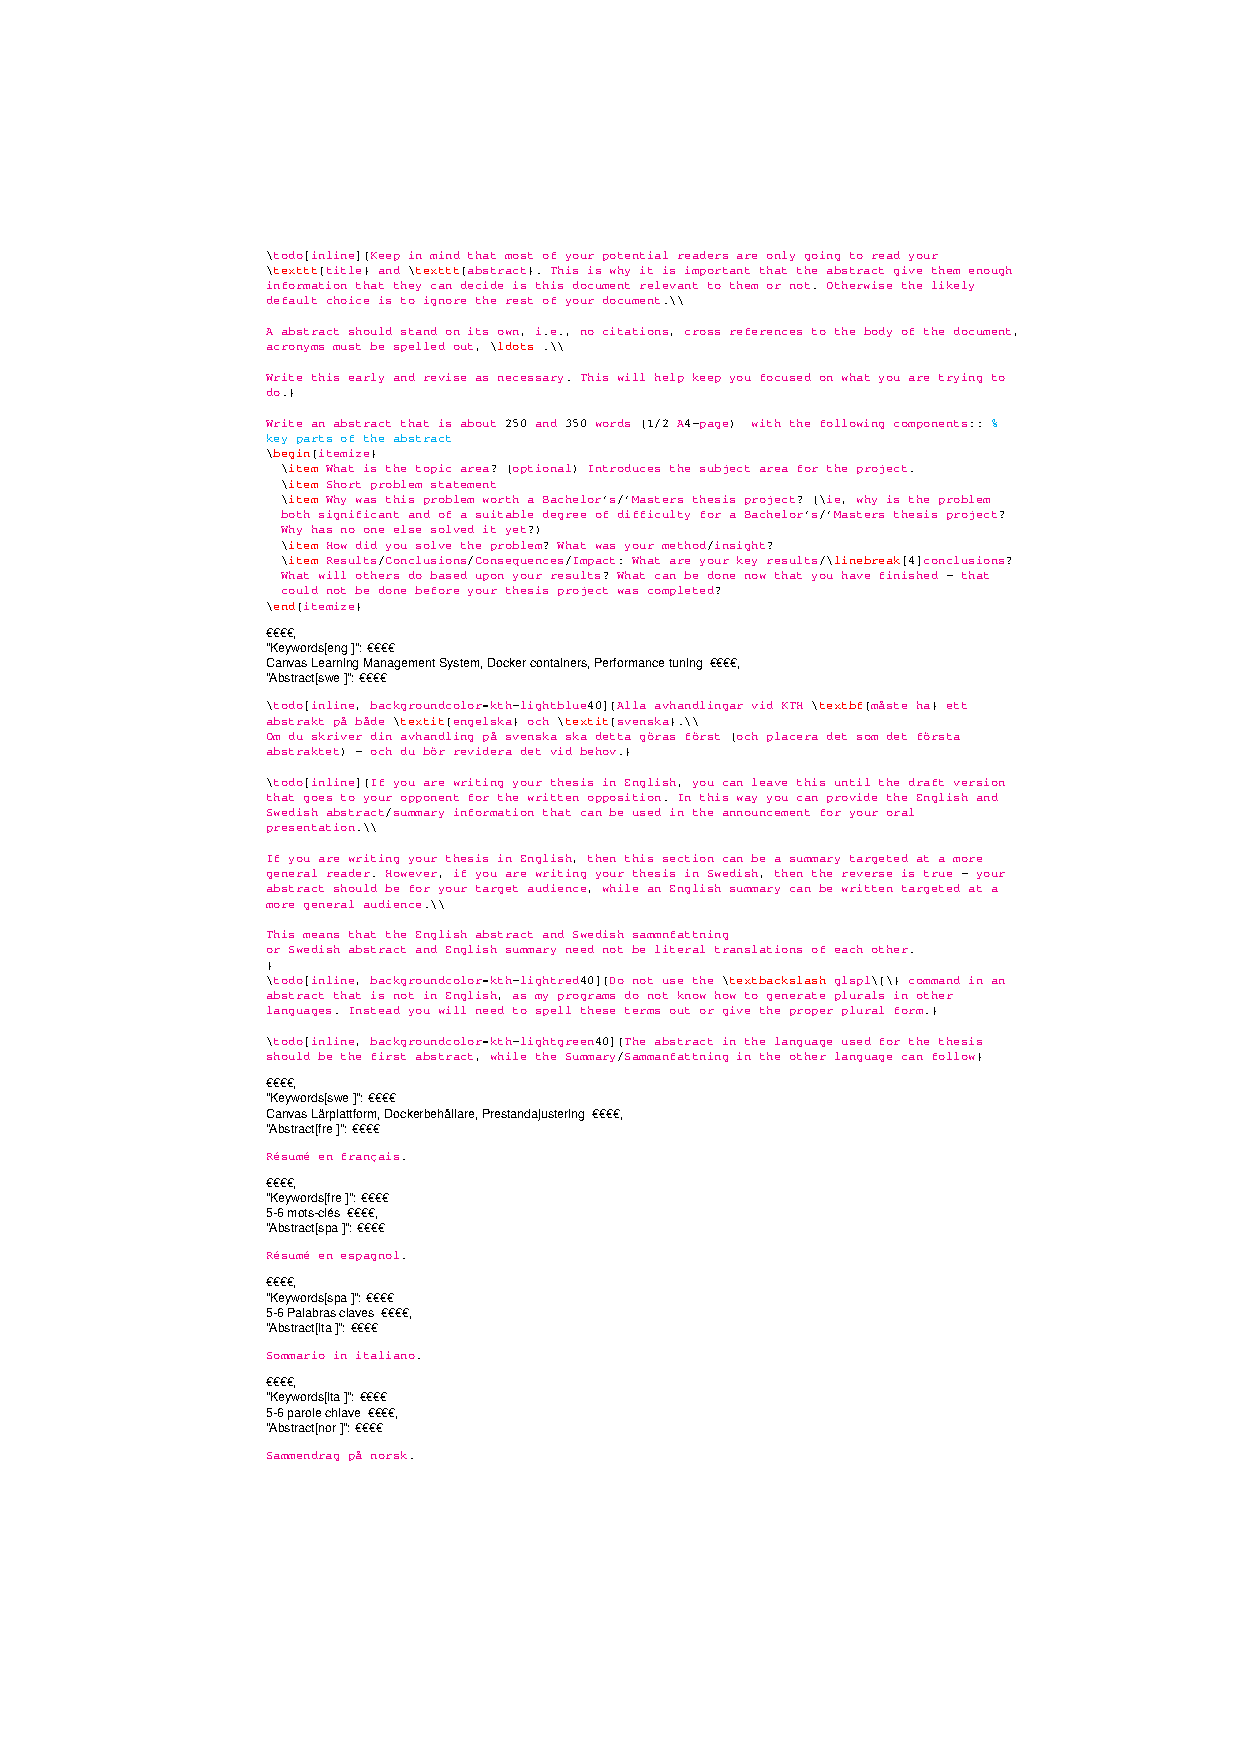
\includegraphics[width=0.80\textwidth]{README_notes/README-examiner-figures/ForDIVA-pg2.pdf}}
  \end{center}
  \caption{Second page of the “For DiVA” information}
  \label{fig:sampleFOrDIVApage2}
\end{figure}
\begin{figure}[!ht]
  \begin{center}
    \fbox{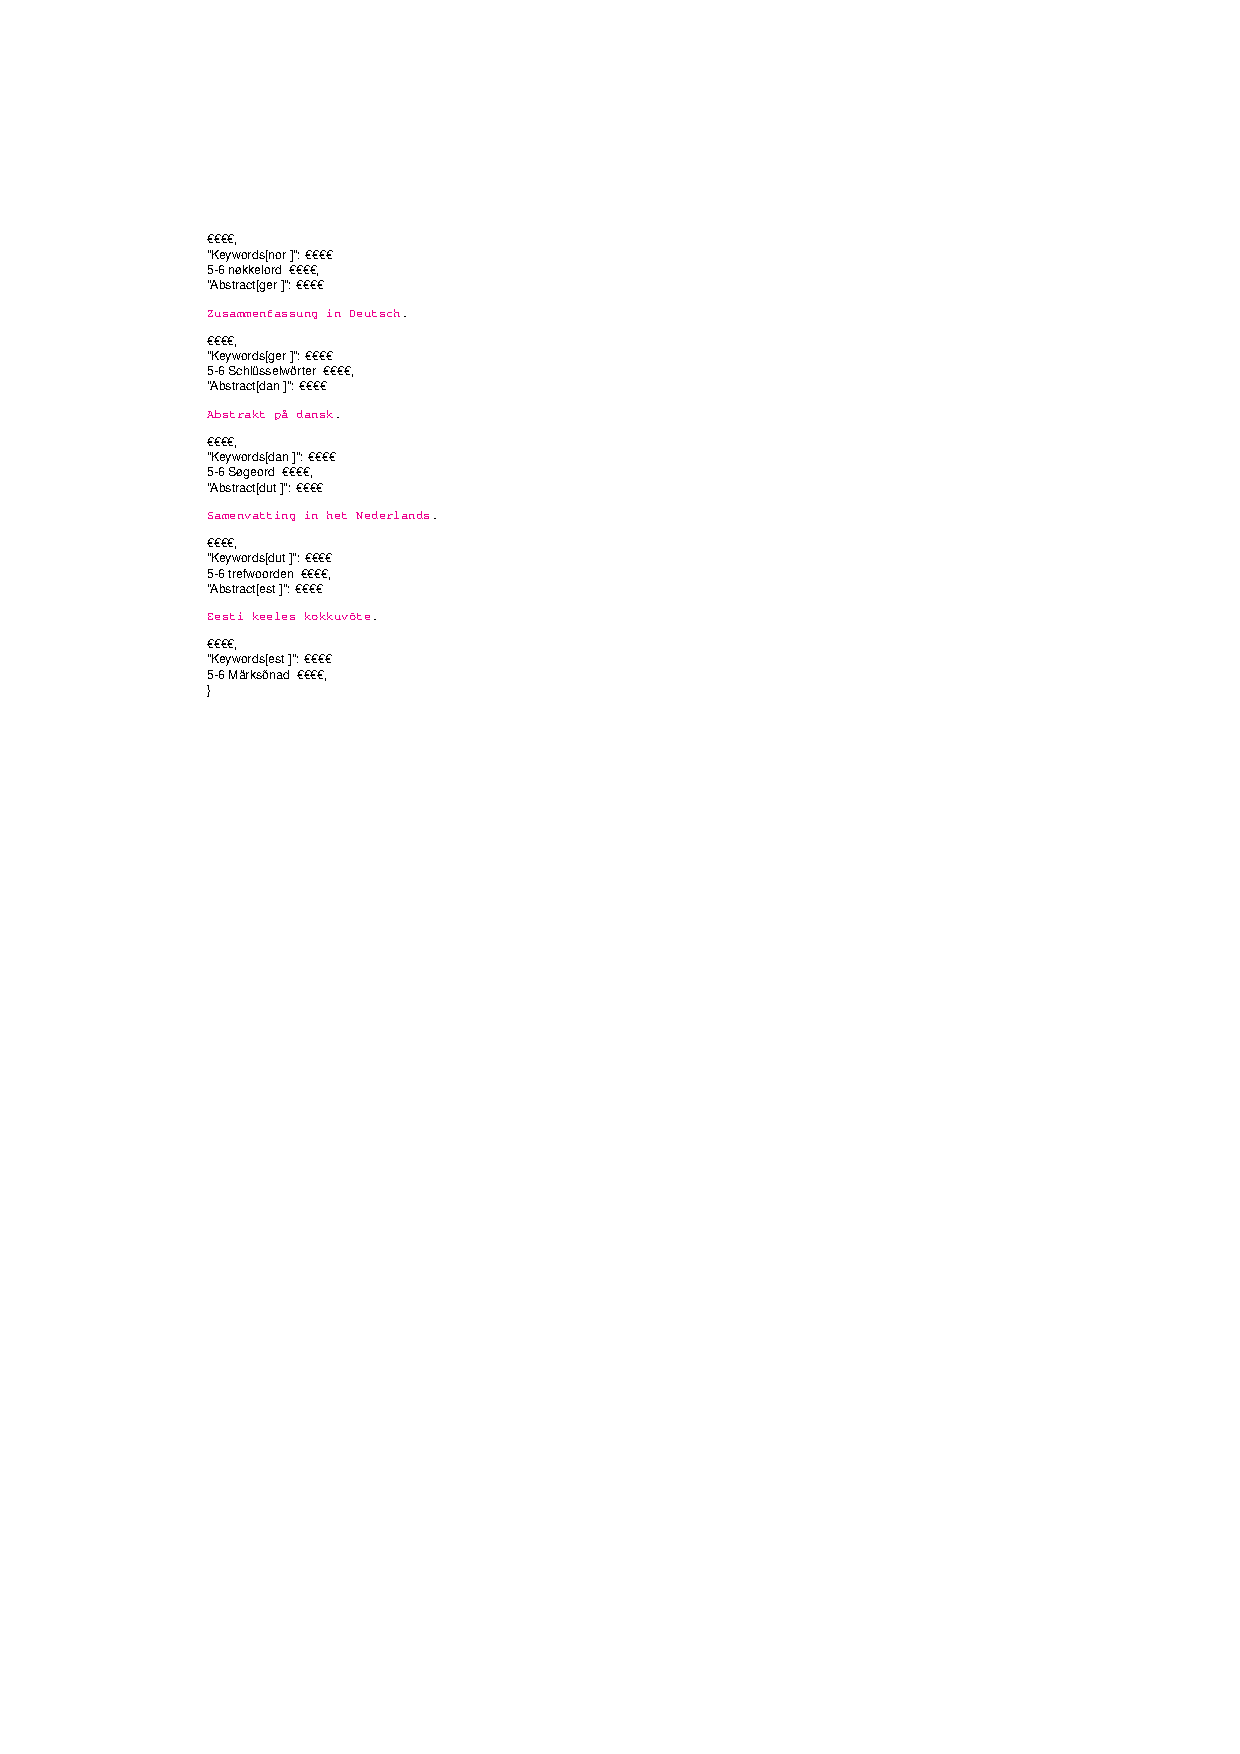
\includegraphics[width=0.80\textwidth]{README_notes/README-examiner-figures/ForDIVA-pg3.pdf}}
  \end{center}
  \caption{Third page of the “For DiVA” information}
  \label{fig:sampleFOrDIVApage3}
\end{figure}
\clearpage
\FloatBarrier


\section{How did the abstracts and the keywords appear?}
\label{sec:scontentsHack}
The \textbackslash divainfo command that generates the For DiVA information pages has the following little bit of code that walks the set of scontents buffers using the lang scontents buffer to put the language and the corresponding abstract and keywords (see \Cref{lst:languages}). Originally, I used \textbackslash getstored[\textbackslash i]{abstracts} to get an abstract, but this turns out to process the \LaTeX~into something to render in the PDF. However, I realized that it would be far better to get the actual \LaTeX~source code and then process it myself into HTML for the announcement and calendars.

The \textbackslash typestored command that the scontents package provides will not take a variable argument, \ie it only takes a constant, such as \textbackslash typestored[2]{abstracts}. Unfortunately, I need to have a loop to handle the variable number of abstracts that could be used. To do this required a new command \textbackslash typestoredx that evaluates the variable and then calls the internal function that gets the contents of the correct scontents buffer! This new command is shown in \Cref{lst:languages} – it uses ExplSyntax – see the \LaTeX~package \texttt{expl3}. The quad euro symbols are used as markers to avoid problems with quotation marks in the abstract itself. I have assumed that such a combination of characters will \textbf{never} occur in an abstract.
\Needspace*{11\baselineskip}
\begin{lstlisting}[language={[LaTeX]TeX}, caption={Code in \textbackslash divainfo command to output the abstracts and keywords }, label=lst:languages] 
    "Number of lang instances": \textquotedbl\relax\countsc{lang}\textquotedbl\relax,\\
    \foreach \i in {1,...,\countsc{lang}} {
      "Abstract[\getstored[\i]{lang}]": €€€€\\
      \typestoredx{\i}{abstracts}
      €€€€,\\
      "Keywords[\getstored[\i]{lang}]": €€€€\\
      \getstored[\i]{keywords}
      €€€€,\\
    }
\end{lstlisting}

\Cref{lst:setupTypestoreedx} shows how to configure the listings environment to put the abstract into. One of the tricks here is that it was important to reduce the hyphenation penalty to enable the abstract text to nicely wrap text on the page. As an added benefit, the \LaTeX~syntax highlighting is on – so one can easily see the \LaTeX~commands that are used – as they might need manual editing before the event is announced. The \LaTeX~code for the English and Swedish abstracts is shown in \Cref{lst:latexAbtractsExampleEnglish} and \Cref{lst:latexAbtractsExampleSwedish} (respectively).

\begin{lstlisting}[language={[LaTeX]TeX}, caption={Code in the document file to set up the command \textbackslash typestoredx and to configure the listing environment to put the abstract into}, label=lst:setupTypestoreedx] 
\ExplSyntaxOn
\newcommand\typestoredx[2]{\expandafter\__scontents_typestored_internal:nn\expandafter{#1} {#2}}
\ExplSyntaxOff
\makeatletter
\let\verbatimsc\@undefined
\let\endverbatimsc\@undefined
\lst@AddToHook{Init}{\hyphenpenalty=50\relax}
\makeatother


\lstnewenvironment{verbatimsc}
    {
    \lstset{%
        basicstyle=\ttfamily\tiny,
        %basicstyle=\tiny,
        %columns=fullflexible,
        columns=[l]fixed,
        language=[LaTeX]TeX,
        %numbers=left,
        %numberstyle=\tiny\color{gray},
        keywordstyle=\color{red},
        breaklines=true,                 % sets automatic line breaking
        breakatwhitespace=true,          % sets if automatic breaks should only happen at whitespace
        %keepspaces=false,
        breakindent=0em,
        %fancyvrb=true
    }
}{}
\end{lstlisting}
\clearpage

\begin{lstlisting}[language={[LaTeX]TeX}, caption={\LaTeX~code for the English abstract}, label=lst:latexAbtractsExampleEnglish] 
\engExpl{All theses at KTH are \textbf{required} to have an
abstract in both \textit{English} and \textit{Swedish}.}
\engExpl{Exchange students many want to include one or more
abstracts in the language(s) used in their home institutions to avoid the need to write another
thesis when returning to their home institution.}
\generalExpl{Keep in mind that most of your potential readers are only going to read your
\texttt{title} and \texttt{abstract}. This is why it is important that the abstract give them enough
information that they can decide if this document is relevant to them or not. Otherwise, the likely
default choice is to ignore the rest of your document.\\
An abstract should stand on its own, i.e., no citations, cross-references to the body of the document,
acronyms must be spelled out, \ldots .\\
Write this early and revise as necessary. This will help keep you focused on what you are trying to
do.}
Write an abstract that is about 250 and 350 words (1/2 A4-page) with the following components:: %
key parts of the abstract
\begin{itemize}
\item What is the topic area? (optional) Introduces the subject area for the project.
\item Short problem statement
\item Why was this problem worth a Bachelor’s/’Masters thesis project? (\ie, why is the problem
both significant and of a suitable degree of difficulty for a Bachelor’s/’Masters thesis project?
Why has no one else solved it yet?)
\item How did you solve the problem? What was your method/insight?
\item Results/Conclusions/Consequences/Impact: What are your key results/\linebreak[4]conclusions?
What will others do based on your results? What can be done now that you have finished - that
could not be done before your thesis project was completed?
\end{itemize}
\end{lstlisting}

\begin{lstlisting}[language={[LaTeX]TeX}, caption={\LaTeX~code for the Swedish abstract}, label=lst:latexAbtractsExampleSwedish]
\todo[inline, backgroundcolor=kth-lightblue40]{Alla avhandlingar vid KTH \textbf{måste ha} ett
abstrakt på både \textit{engelska} och \textit{svenska}.\\
Om du skriver din avhandling på svenska ska detta göras först (och placera det som det första
abstraktet) - och du bör revidera det vid behov.}
\generalExpl{If you are writing your thesis in English, you can leave this until the draft version
that goes to your opponent for the written opposition. In this way you can provide the English and
Swedish abstract/summary information that can be used in the announcement for your oral
presentation.\\
If you are writing your thesis in English, then this section can be a summary targeted at a more
general reader. However, if you are writing your thesis in Swedish, then the reverse is true – your
abstract should be for your target audience, while an English summary can be written targeted at a
more general audience.\\
This means that the English abstract and Swedish sammnfattning
or Swedish abstract and English summary need not be literal translations of each other.
}
\warningExpl{Do not use the \textbackslash glspl\{\} command in an
abstract that is not in English, as my programs do not know how to generate plurals in other
languages. Instead you will need to spell these terms out or give the proper plural form.}
\engExpl{The abstract in the language used for the thesis
should be the first abstract, while the Summary/Sammanfattning in the other language can follow}
\end{lstlisting}

\section{Extracting the information from the PDF file}
Now that the JSON-like information is in the PDF file, the next step is to extract it. The command line shown in \Cref{lst:extractPseudoJSONfromPDF-event} will extract the information. \Cref{lst:JSONfromPDF-event} shows an example of the resulting file.
\begin{lstlisting}[language={bash}, caption={Extract the JSON like information}, label=lst:extractPseudoJSONfromPDF-event]
./extract_pseudo_JSON-from_PDF.py --pdf test5.pdf --json event.json
\end{lstlisting}

\begin{lstlisting}[language={HTML}, caption={Example event.json output (note that this is not the same as currently extracted and note that some lines have been edited and manually broken to overcome limited line length in listing)}, label=lst:JSONfromPDF-event]
{"Author1": {"Last name": "Student", "First name": "Fake A.", "Local User Id": "u100001", "E-mail": "a@kth.se", "organisation": {"L1": "School of XXX"}},
"Author2": {"Last name": "Student", "First name": "Fake B.", "Local User Id": "u100002", "E-mail": "b@kth.se", "organisation": {"L1": "XXX"}},
"Degree": {"Educational program": "Bachelor’s Programme in XXX"},
"Title": {"Main title": "This is the title in the language of the thesis", "Subtitle": "An subtitle in the language of the thesis", "Language": "eng"},
"Alternative title": {"Main title": "Detta är den svenska översättningen av titeln", "Subtitle": "Detta är den svenska översättningen av undertiteln", "Language": "swe"},
"Supervisor1": {"Last name": "Supervisor", "First name": "A. Busy", "Local User Id": "u100003", "E-mail": "sa@kth.se", "organisation": {"L1": "School of XXX", "L2": "DepartmentName"}},
"Supervisor2": {"Last name": "Supervisor", "First name": "Another Busy", "Local User Id": "u100003", "E-mail": "sb@kth.se", "organisation": {"L1": "School of XXX", "L2": "DepartmentName"}},
"Examiner1": {"Last name": "ExaminersLastname", "First name": "ExaminersLastname", "Local User Id": "u100004", "E-mail": "xxx@kth.se", "organisation": {"L1": "School of EXXX", "L2": "DepartmentName"}},
"Cooperation": {"Partner_name": "Företaget AB"}, "Other information": {"Year": "2021", "Number of pages": "xxxiii,35"},
"Opponents": {"Name": "A. B. Normal & A. X. E. Normalè"},
"Presentation": {"Date": "2021-03-16 13:00", "Language": "eng", "Room": "via Zoom", "City": "Stockholm"},
"Number of lang instances": "10",
"abstracts": {"eng": "<p>All theses at KTH are <bold>required</bold> to have an abstract in both <i>English</i> and <i>Swedish</i>.</p><p>Exchange students many want to include one or more abstracts in the language(s) used in their home institutions to avoid the need to write another thesis when returning to their home institution.</p><p>Keep in mind that most of your potential readers are only going to read your <tt>title</tt> and <tt>abstract</tt>. This is why it is important that the abstract give them enough information that they can decide is this document relevant to them or not. Otherwise the likely default choice is to ignore the rest of your document.</p><p>A abstract should stand on its own, i.e., no citations, cross references to the body of the document, acronyms must be spelled out, … .</p><p>Write this early and revise as necessary. This will help keep you focused on what you are trying to do.</p><p>Example of a formula in an abstract: $c=2 \\cdot \\pi \\cdot r$ or \\[ \\int_{a}^{b} x^2 \\,dx \\] two chemical formulas: H<sub>2</sub>O or $(C_5O_2H_8)_n$, copyright symbol: &copy; Maguire 2021, and some superscripts: <sup>99m</sup>Tc, A<sup>*</sup>, A<sup>&reg;</sup>, and A&trade;.</p><p>Write an abstract with the following components: </p><ul><li> What is the topic area? (optional) Introduces the subject area for the project. </li><li> Short problem statement </li><li> Why was this problem worth a ’Masters thesis project? (i.e., why is the problem both significant and of a suitable degree of difficulty for a ’Masters thesis project? Why has no one else solved it yet?) </li><li> How did you solve the problem? What was your method/insight? </li><li> Results/Conclusions/Consequences/Impact: What are your key results/conclusions? What will others do based upon your results? What can be done now that you have finished - that could not be done before your thesis project was completed?</li></ul>",
"swe": "<p>Alla avhandlingar vid KTH måste ha ett abstrakt på både engelska och svenska.</p><p>If you are writing your thesis in English, you can leave this until the final version. If you are writing your thesis in Swedish then this should be done first – and you should revise as necessary along the way.</p><p>If you are writing your thesis in English, then this section can be a summary targeted at a more general reader. However, if you are writing your thesis in Swedish, then the reverse is true – your abstract should be for your target audience, while an English summary can be written targeted at a more general audience.</p><p>This means that the English abstract and Swedish sammnfattning or Swedish abstract and English summary need not be literal translations of each other.</p><p>The abstract in the language used for the thesis should be the first abstract, while the Summary/Sammanfattning in the other language can follow.</p>",
"fre": "<p>Résumé en français.</p>", "spa": "<p>Résumé en espagnol.</p>", "ita": "<p>Sommario in italiano.</p>",
"nor": "<p>Sammendrag på norsk.</p>", "ger": "", "dan": "<p>Abstrakt på dansk.</p><p>Zusammenfassung in Deutsch.</p>",
"dut": "<p>Samenvatting in het Nederlands.</p><p>Eesti keeles kokkuvõte.</p>", "est": ""},
"keywords": {"eng": "Canvas Learning Management System, Docker containers, performance tuning ",
"swe": "Canvas Lärplattform,Dockerbehållare, prestandajustering ", "fre": "5-6 mots-clés ",
"spa": "5-6 Palabras claves ", "ita": "5-6 parole chiave ", "nor": "5-6 nøkkelord ",
"ger": "5-6 Schlüsselwörter ", "dan": "5-6 Søgeord ",
"dut": "5-6 trefwoorden ", "est": "5-6 Märksõnad "}}
\end{lstlisting}
\FloatBarrier

\section{Optimized extraction from an Overleaf LaTeX project}
\label{sec:optimizeJSONToMods}
In the case of an Overleaf project, when compiling the \LaTeX~\ as a side-effect, a \texttt{fordiva.json} file is generated, if you save this file locally, then you can clean it up and make a MODS file with the following commands:
\Needspace*{4\baselineskip}
\begin{lstlisting}[language={bash}, caption={cleanup\_pseudo\_JSON-from\_LaTeX and JSON\_to\_MODS.p},label=lst:cleanPseudoJSONandConvertToMODS]
./cleanup_pseudo_JSON-from_LaTeX.py --json xxx_fordiva.json --acronyms acronyms.tex
./JSON_to_MODS.py --json xxx_fordiva.json
\end{lstlisting}

Now all you have to do is rename the XML file that was produced to \texttt{xxx.mods} and you are all set to upload it into DiVA!

To find the \texttt{fordiva.json} file, look for the “Other logs and files” button shown at the bottom of the log output window. This button is shown in \Cref{fig:otherLogfiles}. After clicking this button you will see a list of log and other files, such as shown in \ref{fig:filesProduced}.
	
\begin{figure}[!ht]
  \begin{center}
    \fbox{
\includegraphics[width=0.80\textwidth]{README_notes/README-examiner-figures/otherlog_files.png}}
  \end{center}
  \caption{Other logs and files button}
  \label{fig:otherLogfiles}
\end{figure}

The details for how the \texttt{fordiva.json} file is generated are given in \Cref{sec:AlternativeWayofGeneratingJSON}.

 \begin{figure}[!ht]
  \begin{center}
    \fbox{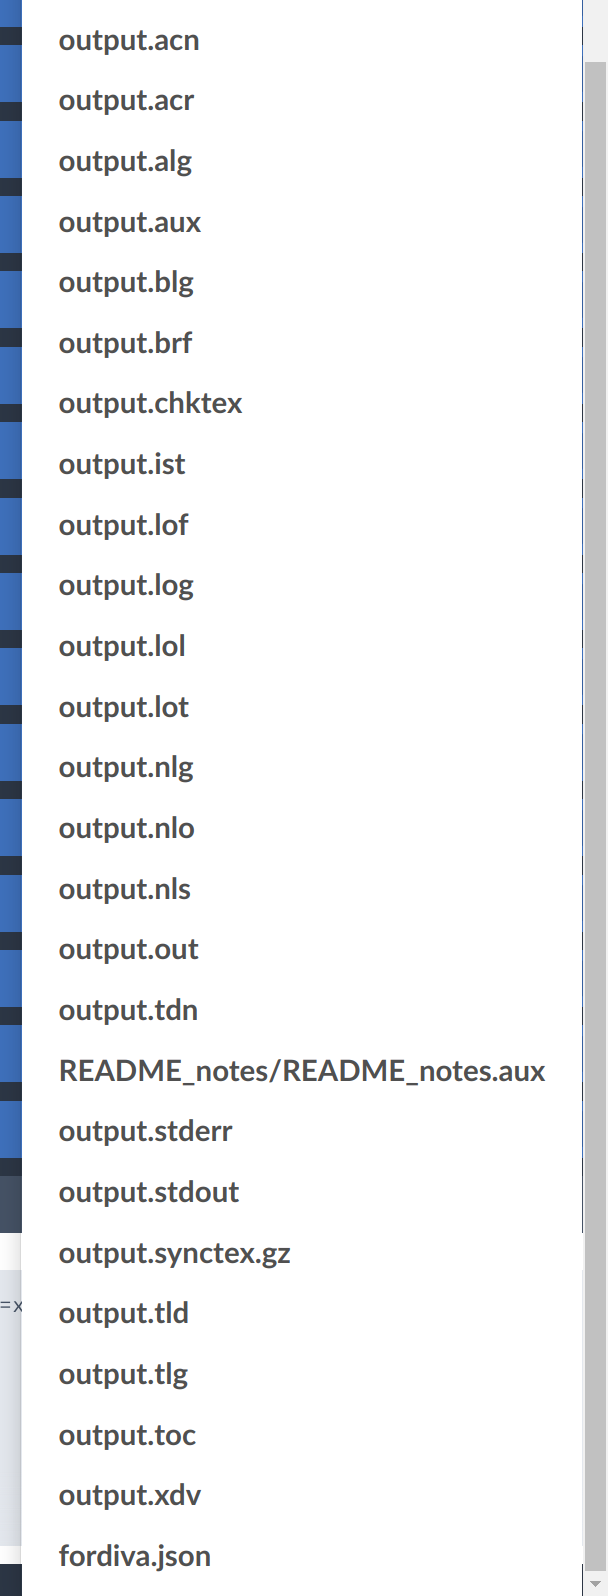
\includegraphics[width=0.50\textwidth]{README_notes/README-examiner-figures/files-produced-Screenshot_20220326_181731.png}}
  \end{center}
  \caption{List of log and other files}
  \label{fig:filesProduced}
\end{figure}
\clearpage

\section{What can we do with the JSON file?}
\label{sec:whatCanweDoWithTheJSONfile}
Now that we have a JSON file, you can edit the HTML in the abstracts to deal with equations and things that were not automatically processed by the extraction program. Once you are happy with the JSON file’s contents, the next step is to generate something interesting with this data – for this we use the program JSON\_to\_calendar.py. 



 \begin{figure}[!ht]
\begin{tikzpicture}
[align=left,node distance=2cm]
\node (jsonFile) [tape,tape bend top=none,draw,font=\sffamily] {JSON file};
\node (start) [processBox, right=1cm of jsonFile] {JSON\_to\_calendar};

\node (calendarEvent) [destinationBox, right=2cm of start] {Canvas calendar event};
\node (announcement) [destinationBox,  above of =calendarEvent] {Canvas announcement};
\node (cortinaCalendarEvent) [destinationBox,  right=0.5cm of start, below of=calendarEvent] {KTH Cortina calendar event};
\draw [arrow] (jsonFile) --  (start.west);
\draw [arrow] (start.east) --  (announcement.west);
\draw [arrow] (start.east) -- (calendarEvent);
\draw [arrow] (start.east) -- (cortinaCalendarEvent.west);

\end{tikzpicture}
\caption{The several outputs of JSON\_to\_calendar.py given a JSON file}
  \label{fig:foo}
\end{figure}
\FloatBarrier

We can produce all three outputs with the command shown in \Cref{lst:JSONtoCalendarThreeoutputs}. Note that the program was run with the \texttt{event.json} file to produce a Canvas course announcement, as shown in \Cref{fig:canvasCourseAnnouncement}. Note that this is being run in the Canvas test instance (hence the pink bar across the bottom of the figure).
\Needspace*{3\baselineskip}
\begin{lstlisting}[language={bash}, caption={Running JSON\_to\_calendar.py to produce all three outputs}, label=lst:JSONtoCalendarThreeoutputs]
JSON_to_calendar.py -c 11 --config config-test.json
\end{lstlisting}

When the cover generator website existed, this same basic mechanism was extended to make and apply the cover for a thesis. There is still a need for a tool that can automate the insertion of the final thesis and metadata into DiVA. While a prototype was shown earlier for this, the IT unit wants to wait for a DiVA API from the DiVA organization. However, an alternative is to generate a MODS file that can be manually imported into DiVA. The process for this will be discussed in \Cref{sec:JSONtoMODSfile}.
\clearpage
\begin{figure}[!ht]
  \begin{center}
    \fbox{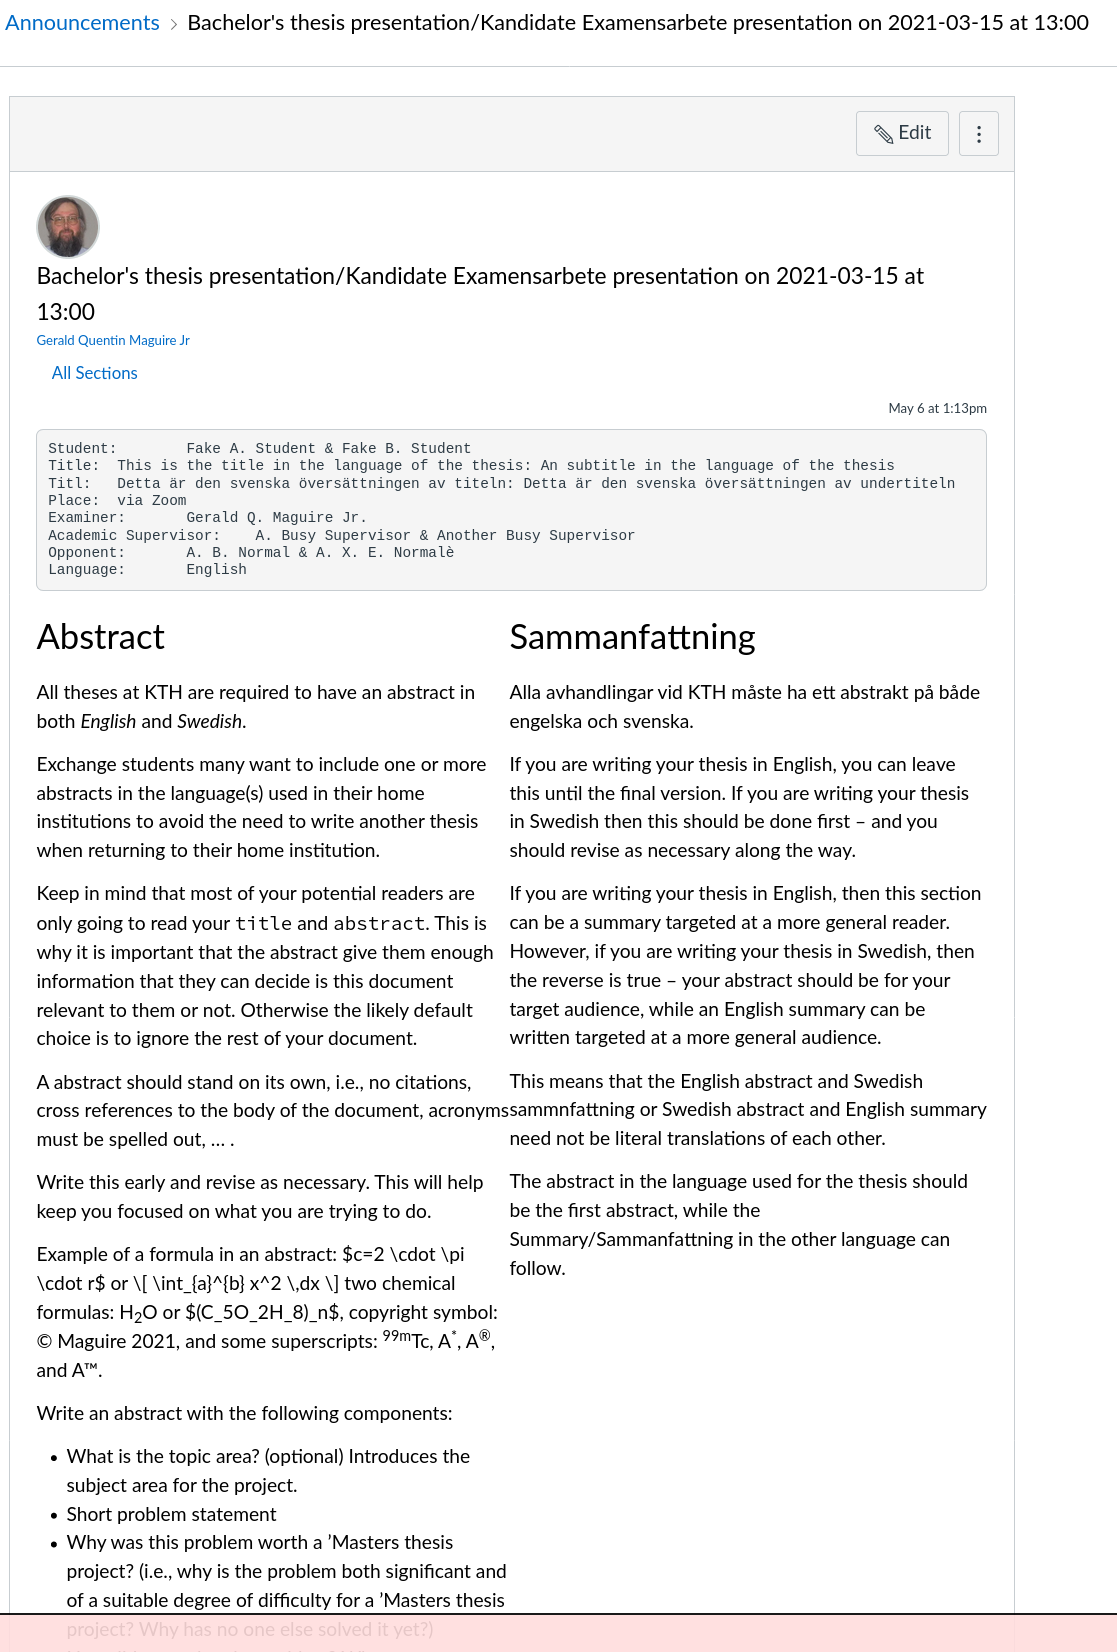
\includegraphics[width=0.99\textwidth]{README_notes/README-examiner-figures/Announcement-in-Canvas-course-Screenshot_20210506_133101.png}}
  \end{center}
  \caption{Canvas course announcement}
  \label{fig:canvasCourseAnnouncement}
\end{figure}
\clearpage
\Cref{fig:canvasCourseAnnouncement} and \Cref{fig:canvasCalendarEvent}  show the event in the Canvas calendar (when I have selected to display the events for course 11 in green).
\begin{figure}[!ht]
  \begin{center}
    \fbox{
\includegraphics[width=0.60\textwidth]{README_notes/README-examiner-figures/Event-in-Canvas-course-calendar-Screenshot_20210506_133011.png}}
  \end{center}
  \caption{A course event in the Canvas calendar (the figure is zoomed in on 15 March 2021}
  \label{fig:canvasCalendarEvent}
\end{figure}

\begin{figure}[!hb]
  \begin{center}
    \fbox{
\includegraphics[width=0.70\textwidth]{README_notes/README-examiner-figures/Canvas-calenda-zoomed-open-event-Screenshot_20210506_163851.png}}
  \end{center}
  \caption{Zoomed view of the opened Canvas calendar event}
  \label{fig:canvasCalendarEventZoomed}
\end{figure}
\newpage

I also edited the \texttt{event.json} to create an event on the following date. The result is two Calendar events as shown in \Cref{fig:cortinaPicture1} in KTH’s Cortina calendar (in this case, it is in the development version of the Polopoly web – as this is the only place where I can use the as of yet unreleased Cortina API which is being developed by KTH’s IT unit. \Cref{fig:cortinaPicture2} and \Cref{fig:cortinaPicture3} show the English and Swedish versions of the event in the calendar.s

\begin{figure}[!ht]
  \begin{center}
    \fbox{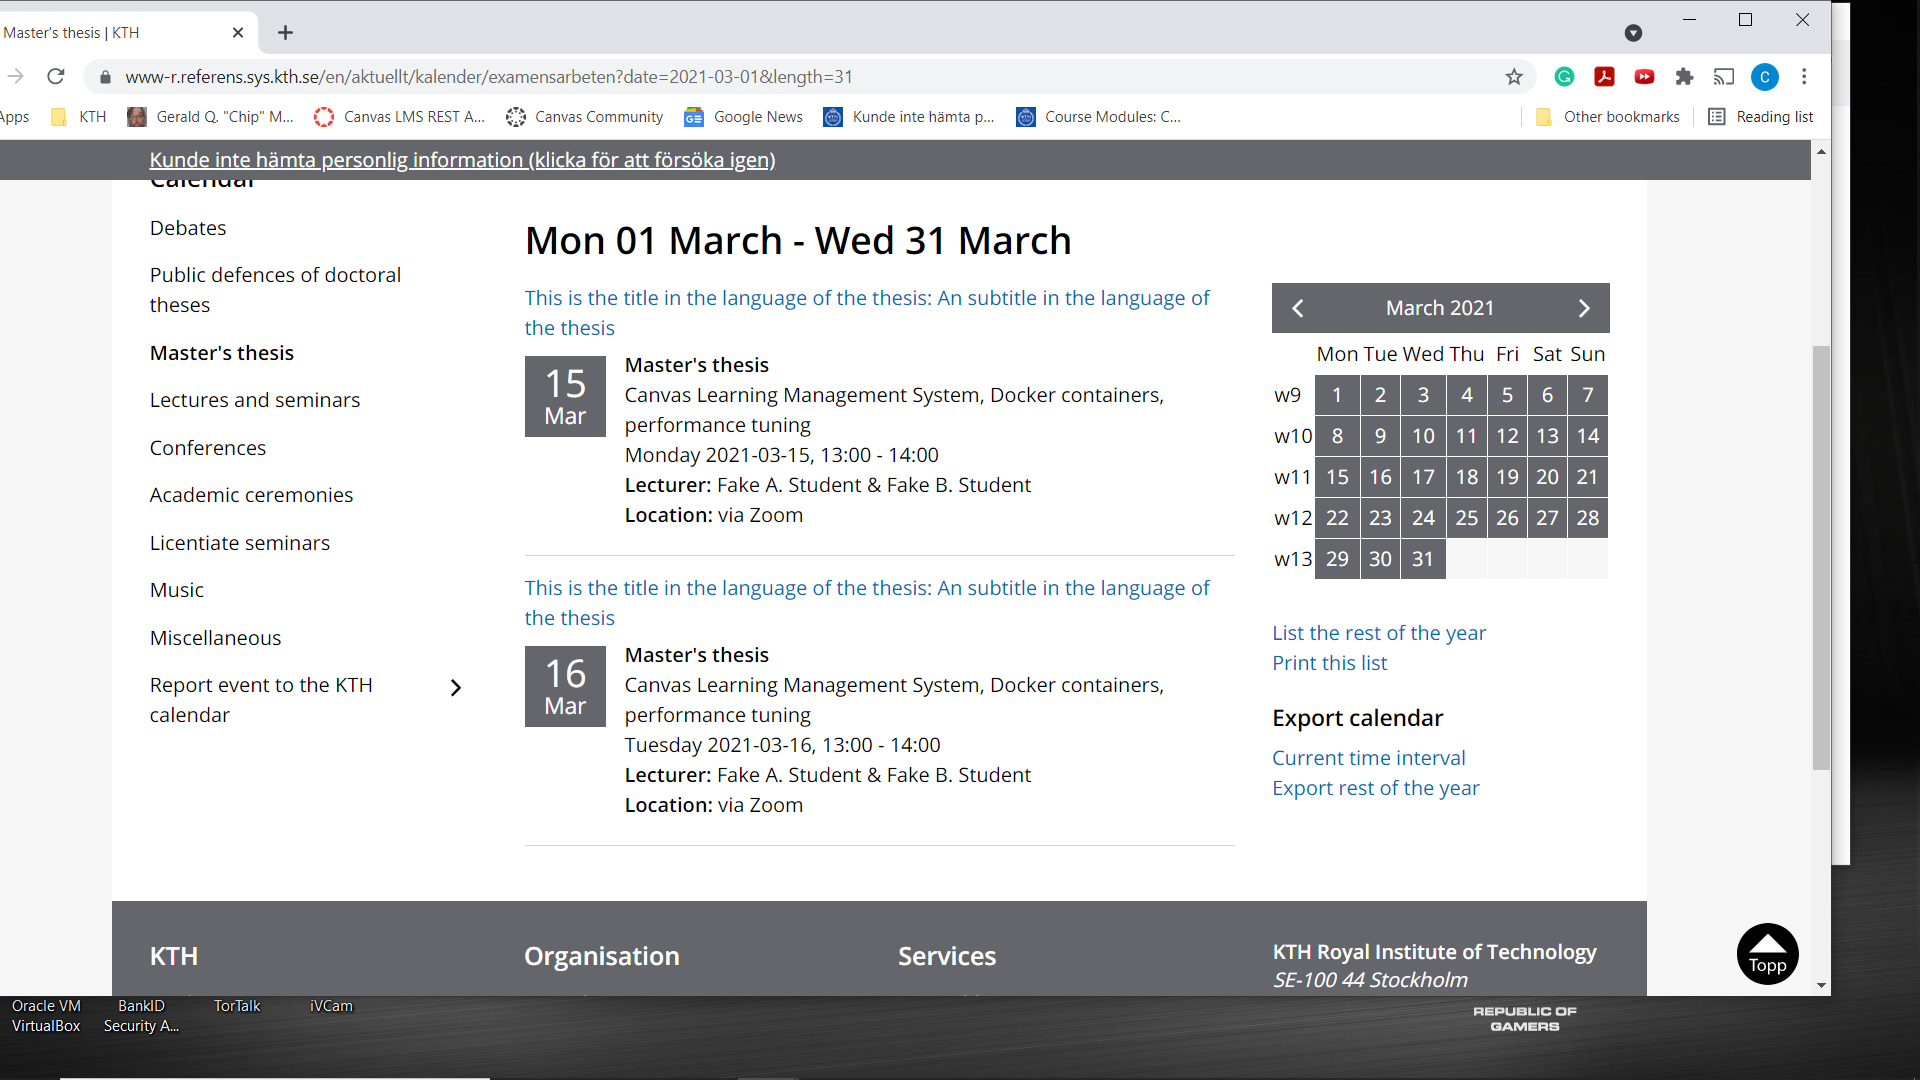
\includegraphics[width=0.99\textwidth, trim=3cm 2cm 8cm 0.2cm, clip]{README_notes/README-examiner-figures/cortina-2021-03-16-picture.png}}
  \end{center}
  \caption{KTH’s Cortina calendar showing two degree project events}
  \label{fig:cortinaPicture1}
\end{figure}
\FloatBarrier

\begin{figure}[!ht]
  \begin{center}
    \fbox{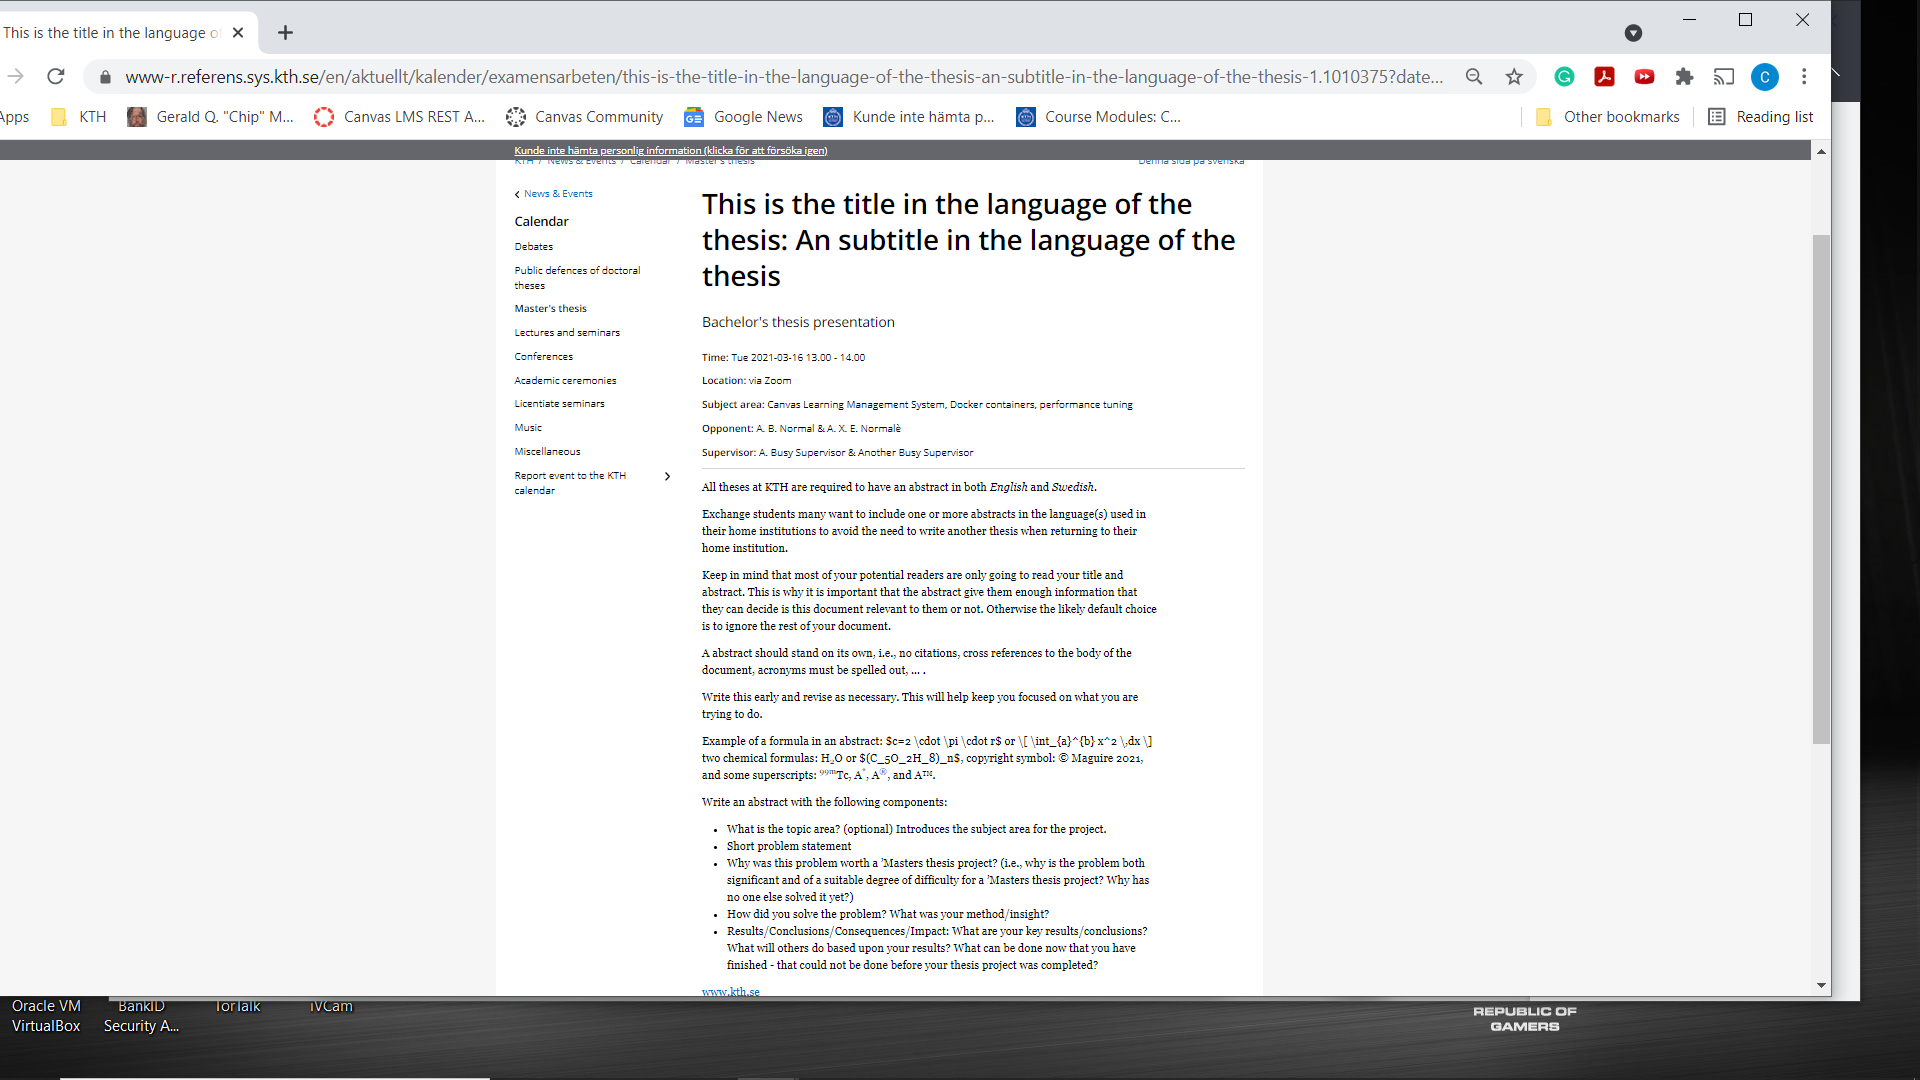
\includegraphics[width=1.0\textwidth, trim=3cm 2cm 16cm 0.2cm, clip]{README_notes/README-examiner-figures/cortina-2021-03-16-picture2.png}}
  \end{center}
  \caption{English version of the calendar}
  \label{fig:cortinaPicture2}
\end{figure}
\FloatBarrier	

\begin{figure}[!ht]
  \begin{center}
    \fbox{
\includegraphics[width=1.0\textwidth, trim=3cm 2cm 16cm 0.2cm, clip]{README_notes/README-examiner-figures/cortina-2021-03-16-picture3.png}}
  \end{center}
  \caption{Swedish version of the calendar}
  \label{fig:cortinaPicture3}
\end{figure}
\FloatBarrier

\Cref{lst:cortinaResponse} shows the response from doing a POST to the KTH Cortina API. Note that this is a prototype and as of the date of my experiments did not yet support having an examiner in a calendar event (hence I had to save and remove this element of the dict before passing the data to the API, then I restored this element for use by the subsequent routines).

\begin{lstlisting}[language={json}, caption={Response from the KTH Cortina API},label=lst:cortinaResponse]
{
  "advisor": "A. Busy Supervisor & Another Busy Supervisor",
  "contentId": "1.1010375",
  "contentName": {
    "en_GB": "This is the title in the language of the thesis: An subtitle in the language of the thesis",
    "sv_SE": "Detta är den svenska översättningen av titeln: Detta är den svenska översättningen av undertiteln"
  },
  "dates_endtime": "2021-03-16T13:00:00.000Z",
  "dates_starttime": "2021-03-16T12:00:00.000Z",
  "lead": {
    "en_GB": "Bachelor's thesis presentation",
    "sv_SE": "Kandidate Examensarbete presentation"
  },
  "lecturer": "Fake A. Student & Fake B. Student",
  "location": "via Zoom",
  "opponent": "A. B. Normal & A. X. E. Normalè",
  "organisation": {
    "school": "XXX",
    "department": "DepartmentName"
  },
  "respondent": "",
  "respondentDepartment": "",
  "subjectarea": {
    "en_GB": "KeywordA, KeywordB, KeywordC",
    "sv_SE": "NyckelordA, NyckelordB, NyckelordC"
  },
  "seminartype": "thesis",
  "paragraphs_text": {
    "en_GB": "<p>All theses at KTH are required to have an abstract in both <i>English</i> and <i>Swedish</i>.</p> \n<p>Exchange students many want to include one or more abstracts in the language(s) used in their home institutions to avoid the need to write another thesis when returning to their home institution.</p> \n<p>Keep in mind that most of your potential readers are only going to read your title and abstract. This is why it is important that the abstract give them enough information that they can decide is this document relevant to them or not. Otherwise the likely default choice is to ignore the rest of your document.</p> \n<p>A abstract should stand on its own, i.e., no citations, cross references to the body of the document, acronyms must be spelled out, … .</p> \n<p>Write this early and revise as necessary. This will help keep you focused on what you are trying to do.</p> \n<p>Example of a formula in an abstract: $c=2 \\cdot \\pi \\cdot r$ or \\[ \\int_{a}^{b} x^2 \\,dx \\] two chemical formulas: H<sub>2</sub>O or $(C_5O_2H_8)_n$, copyright symbol: © Maguire 2021, and some superscripts: <sup>99m</sup>Tc, A<sup>*</sup>, A<sup>®</sup>, and A™.</p> \n<p>Write an abstract with the following components: </p> \n<ul> \n <li> What is the topic area? (optional) Introduces the subject area for the project. </li> \n <li> Short problem statement </li> \n <li> Why was this problem worth a ’Masters thesis project? (i.e., why is the problem both significant and of a suitable degree of difficulty for a ’Masters thesis project? Why has no one else solved it yet?) </li> \n <li> How did you solve the problem? What was your method/insight? </li> \n <li> Results/Conclusions/Consequences/Impact: What are your key results/conclusions? What will others do based upon your results? What can be done now that you have finished - that could not be done before your thesis project was completed?</li> \n</ul>\n",
    "sv_SE": "<p>Alla avhandlingar vid KTH måste ha ett abstrakt på både engelska och svenska.</p> \n<p>If you are writing your thesis in English, you can leave this until the final version. If you are writing your thesis in Swedish then this should be done first – and you should revise as necessary along the way.</p> \n<p>If you are writing your thesis in English, then this section can be a summary targeted at a more general reader. However, if you are writing your thesis in Swedish, then the reverse is true – your abstract should be for your target audience, while an English summary can be written targeted at a more general audience.</p> \n<p>This means that the English abstract and Swedish sammnfattning or Swedish abstract and English summary need not be literal translations of each other.</p> \n<p>The abstract in the language used for the thesis should be the first abstract, while the Summary/Sammanfattning in the other language can follow.</p>\n"
  },
  "uri": "https://www.kth.se"
}
\end{lstlisting}


\section{Actual example}
This example appears with the student’s permission. \Cref{fig:actualAnnouncementTop} shows the announcement for a second-cycle thesis presentation in a Canvas course while \Cref{fig:actualAnnouncementBottom} shows the bottom part of the announcement. \Cref{fig:actualCalendarOpenned} shows the opened Canvas course calendar entry while \Cref{fig:actualEnglishAndSwedish} shows the Cortina calendar entry. Note that the Cortina calendar entry is in the development system and not the production calendar. \Cref{lst:extractPseudoAndJSONtoCalendar} shows the command to extract the JSON information from the student’s PDF file and then the command to make the announcement and calendar entries. \Cref{lst:extractedPseudoAndJSONtoCalendar} shows the extracted JSON.

Note that the entry was made on 2021-06-17, but the event was earlier. This entry was made with the new (as of this date) KTH Cortina Calendar API that supports the examiner and language of presentation fields. Additionally, it returns a canonicalUrl (the URL to this calendar entry). The program was extended to add this URL to the course announcement and course calendar entry.

\begin{figure}[!ht]
  \begin{center}
    \fbox{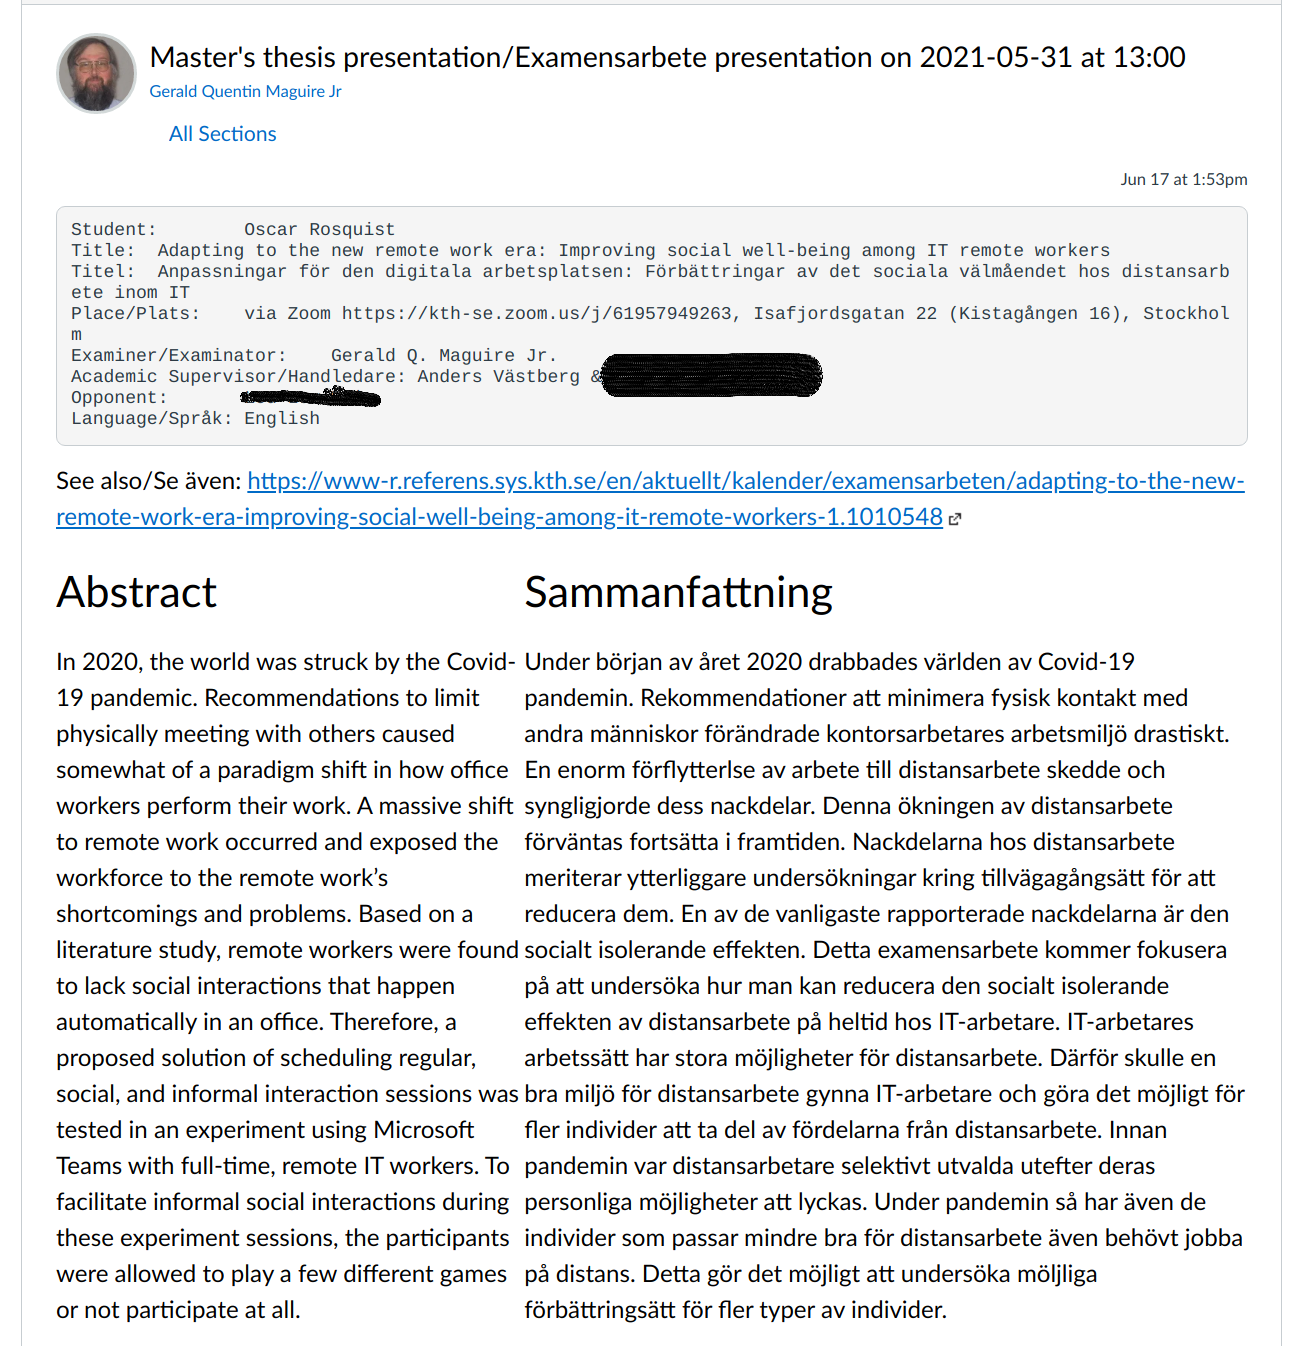
\includegraphics[width=1.2\textwidth]{README_notes/README-examiner-figures/Oscar-1-Screenshot_20210617_140037.png}}
  \end{center}
  \caption{Actual example of announcement in Canvas (top)}
  \label{fig:actualAnnouncementTop}
\end{figure}
\FloatBarrier

\begin{figure}[!ht]
  \begin{center}
    \fbox{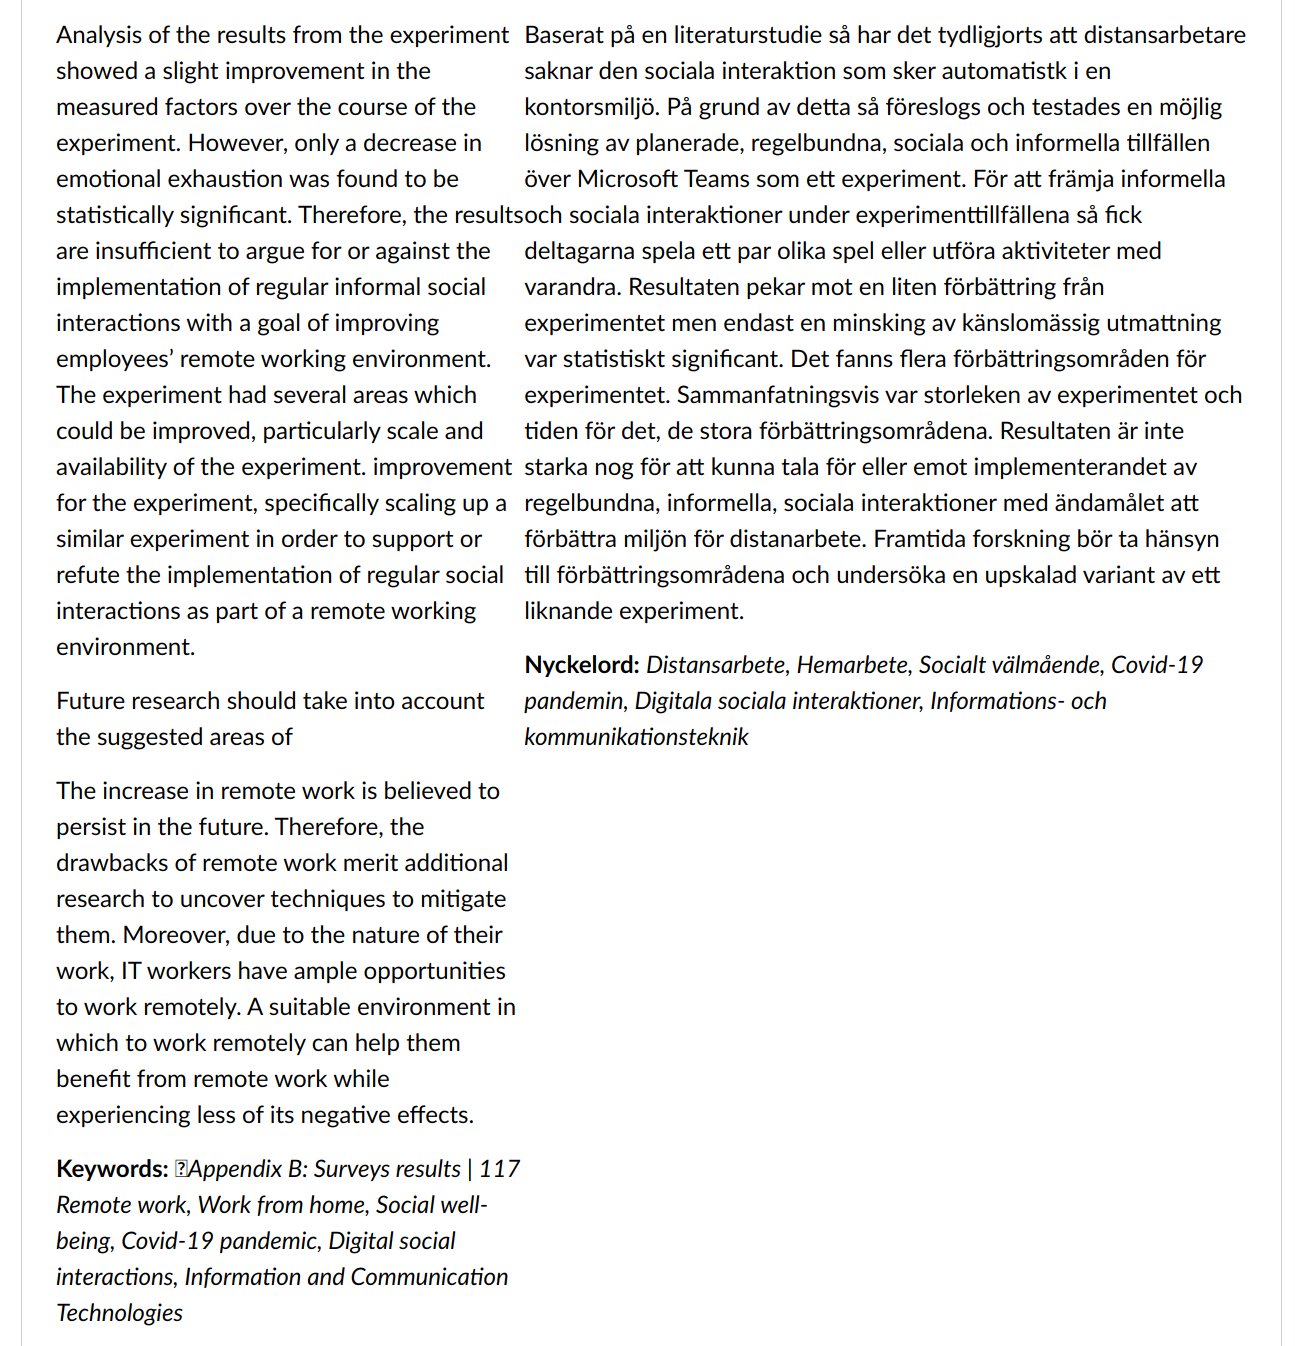
\includegraphics[width=1.2\textwidth]{README_notes/README-examiner-figures/Oscar-2-Screenshot_20210617_140116.png}}
  \end{center}
  \caption{Bottom of the announcement}
  \label{fig:actualAnnouncementBottom}
\end{figure}
\FloatBarrier
	
\begin{figure}[!ht]
  \begin{center}
    \fbox{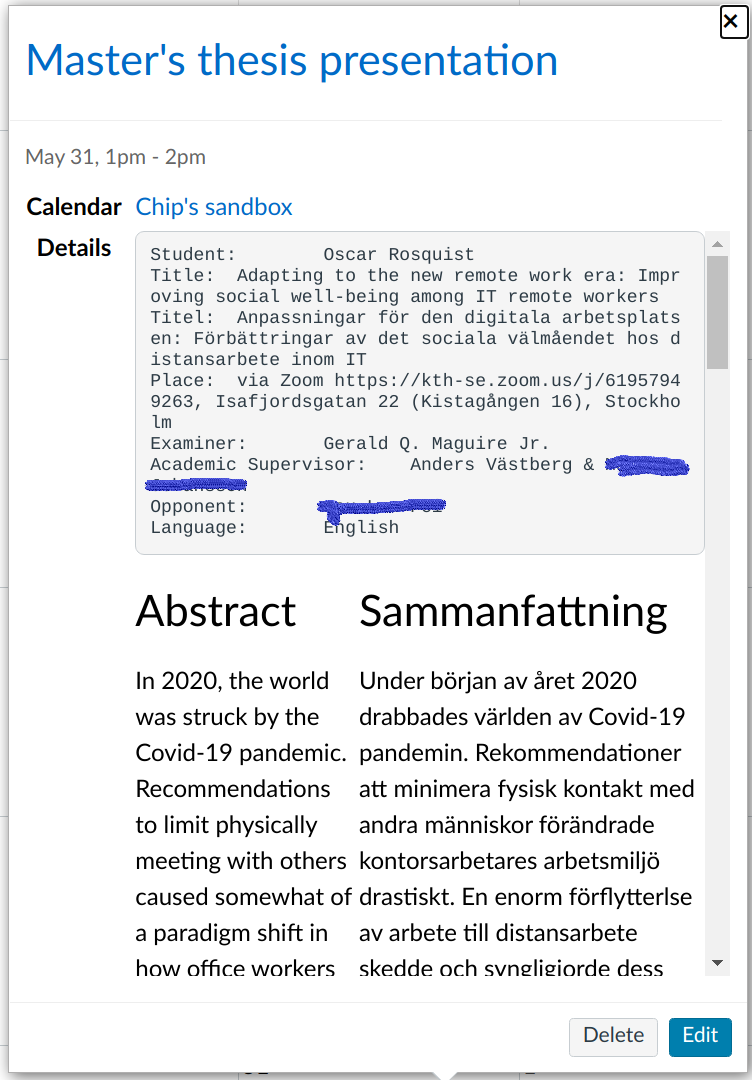
\includegraphics[width=1\textwidth]{README_notes/README-examiner-figures/oscar-course-calendar-Screenshot_20210617_143054.png}}
  \end{center}
  \caption{Opened version in course calendar}
  \label{fig:actualCalendarOpenned}
\end{figure}
\FloatBarrier	

\begin{figure}[!ht]
  \begin{center}
  \begin{subfigure}{0.45\textwidth}
    \fbox{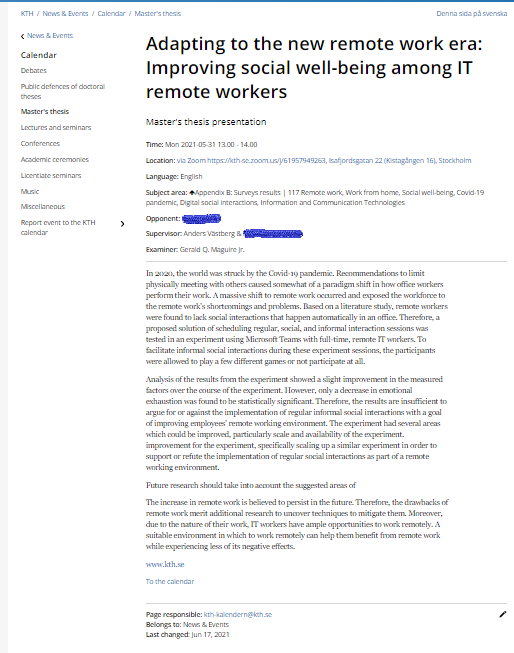
\includegraphics[width=\textwidth]{README_notes/README-examiner-figures/oscar-english-cortina.png}}
    \caption{English}
   \end{subfigure}
   \begin{subfigure}{0.45\textwidth}
    \fbox{
\includegraphics[width=\textwidth]{README_notes/README-examiner-figures/oscar-swedish-cortina.png}}
    \caption{Swedish}
  \end{subfigure}
  \end{center}
  \caption{The English (left) and Swedish (right) in the Cortina calendar}
  \label{fig:actualEnglishAndSwedish}
\end{figure}
\newpage

\Needspace*{4\baselineskip}
\begin{lstlisting}[language={bash}, caption={Commands to extract the JSON and to make the calendar entries and announcements}, label=lst:extractPseudoAndJSONtoCalendar]
./extract_pseudo_JSON-from_PDF.py --pdf oscar.pdf --json oscar.json
./JSON_to_calendar.py -c 11 --config config-test.json --json oscar.json
\end{lstlisting}

\begin{lstlisting}[language={json}, caption={Extracted JSON file oscar.json - edited for appearance here}, label=lst:extractedPseudoAndJSONtoCalendar]
{"Author1": {"Last name": "StudentsLastname", "First name": "StudentsLastname", "Local User Id": "u1000000", "E-mail": "oscarros@kth.se", "organisation": {"L1": "School of XXX"}}, "Degree": {"Educational program": "Degree Programme in XXX"},
"Title": {"Main title": "Adapting to XXX", "Subtitle": "Improving XXX", "Language": "eng"},
"Alternative title": {"Main title": "Anpassningar för XXX", "Subtitle": "Förbättringar av XXX", "Language": "swe"},
"Supervisor1": {"Last name": "Västberg", "First name": "Anders", "Local User Id": "u1ft3a12", "E-mail": "vastberg@kth.se", "organisation": {"L1": "School of XXX", "L2": "StudentsLastname"}},
"Supervisor2": {"Last name": "XXXXX", "First name": "XXXXX", "E-mail": "XXXXXX", "Other organisation": "XXXXX"},
"Examiner1": {"Last name": "ExaminersLastname", "First name": "ExaminersFirstname", "Local User Id": "u1000000", "E-mail": "xxx@kth.se", "organisation": {"L1": "School of XXX", "L2": "DepartmentName"}},
"Cooperation": {"Partner_name": "XXXXX"},
"Other information": {"Year": "2021", "Number of pages": "xvii,115"},
"Opponents": {"Name": "XXXXXX"}, "Presentation": {"Date": "2021-05-31 13:00", "Language": "eng", "Room": "via Zoom https://kth-se.zoom.us/j/61957949263", "Address": "Isafjordsgatan 22 (Kistagången 16)", "City": "Stockholm",
"National Subject Categories": "10201, 10206"}, "Number of lang instances": "2", "abstracts": {"eng": "<p>In 2020, the world was struck by the Covid-19 pandemic. …negative effects.</p>",
"swe": "<p>Under början av året 2020 drabbades världen av Covid-19 pandemin. … ett liknande experiment.</p>"},
"keywords": {"eng": "\n\fAppendix B: Surveys results | 117\n\nRemote work, Work from home, Social well-being, Covid-19 pandemic, Digital social interactions, Information and Communication\nTechnologies ",
"swe": "Distansarbete, Hemarbete, Socialt välmående, Covid-19 pandemin, Digitala sociala interaktioner, Informations- och kommunikationsteknik\n"}}	
\end{lstlisting}


\section{Change in how to enter the abstracts in \LaTeX}
In order to deal with both Babel and Polyglossia and both bibtex and biblatex, I have changed how the abstracts should be entered. Basically the idea is to insert a \textbackslash babelpolyLangStart \{language\_name\}  before the start of the abstract and \textbackslash babelpolyLangStop after the end of the abstract. These commands hide the difference between using Babel or Polyglossia. Additionally, they avoid the problem of the Overleaf GUI being confused about matching beginning and ending statements. \Cref{lst:babel} and \Cref{lst:babelSecondExample} show examples of how to enter an abstract and keywords while \Cref{lst:babelCMDS} shows the definition of the two commands.

Note that both Babel and Polyglossia expand the \textbackslash abstractname into the correct version of the name for an abstract in the current language. Unfortunately, neither package has an equivalent to provide the language specific version of “keywords”, so these have to be provided by the person entering the keywords. For example writing \textbackslash subsection*\{Nyckelord\} to have the Swedish word for keywords set as the subsection heading.

\begin{lstlisting}[language={[LaTeX]TeX}, caption={Example of the revised format for entering an abstract}, label=lst:babel]
\babelpolyLangStart{swedish}
\begin{abstract}
    \markboth{\abstractname}{}
\begin{scontents}[store-env=lang]
swe
\end{scontents}
\begin{scontents}[store-env=abstracts,print-env=true]
Alla avhandlingar vid KTH måste ha ett abstrakt på både engelska och svenska.

Om du skriver din avhandling på svenska ska detta göras först (och placera det som det första abstraktet) - och du bör revidera det vid behov.

If you are writing your thesis in English, you can leave this until the draft version that goes to your opponent for the written opposition. In this way you can provide the English and Swedish abstract/summary information that can be used in the announcement for your oral presentation.

If you are writing your thesis in English, then this section can be a summary targeted at a more general reader. However, if you are writing your thesis in Swedish, then the reverse is true – your abstract should be for your target audience, while an English summary can be written targeted at a more general audience.

This means that the English abstract and \foreignlanguage{swedish}{sammnfattning} 
or Swedish abstract and English summary need not be literal translations of each other.

The abstract in the language used for the thesis should be the first abstract, while the Summary/Sammanfattning in the other language can follow.
\end{scontents}
\subsection*{Nyckelord}
\begin{scontents}[store-env=keywords,print-env=true]
Canvas Lärplattform,Dockerbehållare, prestandajustering
\end{scontents}
\end{abstract}
\babelpolyLangStop{swedish}
\end{lstlisting}
	

\begin{lstlisting}[language={[LaTeX]TeX}, caption={Second example of the revised format for entering an abstract}, label=lst:babelSecondExample]
\generalExpl{Use the relevant language for abstracts for your home university.\\
Note that you may need to augment the set of language used in polyglossia or
babel (see the file kththesis.cls). The following languages include those languages that were used in theses at KTH in 2018-2019, except for one in Chinese.\\
Remove those versions that you do not need.\\
If adding a new language, when specifying the language for the abstract use the three-letter ISO 639-2 Code – specifically the "B" (bibliographic) variant of these codes (note that this is the same language code used in DiVA).
\babelpolyLangStart{french}
\begin{abstract}
    \markboth{\abstractname}{}
\begin{scontents}[store-env=lang]
fre
\end{scontents}
\begin{scontents}[store-env=abstracts,print-env=true]
Résumé en français.
\end{scontents}
\subsection*{Mots clés}
\begin{scontents}[store-env=keywords,print-env=true]
5-6 mots-clés
\end{scontents}
\end{abstract}
\babelpolyLangStop{french}
\cleardoublepage
\end{lstlisting}
\Needspace*{12\baselineskip}
\begin{lstlisting}[language={[LaTeX]TeX}, caption={The two commands used to help enter the language specification}, label=lst:babelCMDS]
\ifxeorlua
    \newcommand{\babelpolyLangStop}[1]{\end{#1}}
\else
    \newcommand{\babelpolyLangStop}[1]{\end{otherlanguage}}
\fi

\ifxeorlua
   \newcommand{\babelpolyLangStart}[1]{\begin{#1}}
\else
    \newcommand{\babelpolyLangStart}[1]{\begin{otherlanguage}{#1}}
\fi
\end{lstlisting}


\section{Adding keywords and PDF metadata}
\label{sec:addingKeywordsAndMetaDataToPDF}
In an effort to add the PDF metadata via the \texttt{hyperref} package, I also decided to add the keywords part of the PDF metadata. However, in order to do this I had to have the keywords \textit{before} the \textbackslash begin\{document\} command in the \LaTeX~file. To do so, I added three new commands to the \texttt{kththesis.cls} file, as shown in \Cref{lst:keywords}. The commands are used in the \texttt{examplethesis.tex} file to set up the keywords in both English and Swedish as well as include a new set of \LaTeX~commands to store the PDF metadata (as shown in \Cref{lst:storingkeywords}) using a file called \texttt{lib/pdf\_related\_includes.tex} (shown in \Cref{lst:informationforPDFfile}). Later the keywords that have been stored are inserted into the \LaTeX~after their respective language abstracts as shown in \Cref{lst:keywordsSection} and \Cref{lst:keywordsSectionSwedish}. The title page of the thesis and the PDF metadata are shown in \Cref{fig:pdfMetadata}. Note that both the English and Swedish version of the keywords are included in the metadata. Finally, the keywords appear (as expected) in the For DiVA data at the end of the PDF file as shown in \Cref{lst:keywordsFromForDIVA}.

Note that \textbackslash makeatletter and \textbackslash makeatother are use to include the character “@” as a letter and then return “@” to being a punctuation code. This use of “@” protects the internal names from being accessed outside of these two commands. More explicitly, \textbackslash EnglishKeywords is a function that takes one argument, the text of the English keywords, and then stores them into “@EnglishKeywords”. Later the text can be retrieved with the command \textbackslash InsertKeywords\{english\} or \textbackslash InsertKeywords\{swedish\}.
\Needspace*{15\baselineskip}
\begin{lstlisting}[language={[LaTeX]TeX}, caption={New commands in kththesis.cls}, label=lst:keywords]
% Keywords
\let\@EnglishKeywords\@empty
\newcommand{\EnglishKeywords}[1]{\def\@EnglishKeywords{#1}}

\let\@SwedishKeywords\@empty
\newcommand{\SwedishKeywords}[1]{\def\@SwedishKeywords{#1}}

\makeatletter
\newcommand{\InsertKeywords}[1]{
    \IfEqCase{#1}{%
    {english}{\@EnglishKeywords}
    {swedish}{\@SwedishKeywords}
  }[\typeout{argument must be english or swedish}]
}
\end{lstlisting}

\Cref{lst:storingkeywords} shows the storing of the keywords using the above commands and the include of the library to set up the PDF metadata.
\Needspace*{10\baselineskip}
\begin{lstlisting}[language={[LaTeX]TeX}, caption={shows the storing of the keywords using the above commands and the include of the library to set up the PDF meta data}, label=lst:storingkeywords]
% Enter the English and Swedish keywords here for use in the PDF meta data _and_ for later use
% following the respective abstract.
% Try to put the words in the same order in both to facilitate matching.
\EnglishKeywords{Canvas Learning Management System, Docker containers, performance tuning}
\SwedishKeywords{Canvas Lärplattform, Dockerbehållare, prestandajustering}

% Put the title, author, and keyword information into the PDF meta information
% This file contains the LaTeX to add information to the PDF file (specifically, author(s), title(s), and keywords
% It uses the hyperref package and should be included before the \begin{document}
%
% I want to acknowledge the inspiration of Karl Voit's template for TU Graz that inspired me to add the PDF document information
% For more information about his template see https://github.com/novoid/LaTeX-KOMA-template
% Note that this template does not use anything from his template other than the names of the information for the PDF meta fields, i.e., mytitle, myauthor, and mykeywords together with the idea of defining the corresponding newcommand to set the relevant hyperref parameters.

\makeatletter
\ifx\@subtitle\@empty
    \newcommand{\mytitle}{\@title}
\else
    \ifinswedish
        \newcommand{\mytitle}{\@title\xspace–\xspace\@subtitle}
    \else
        \newcommand{\mytitle}{\@title: \@subtitle}
    \fi
\fi
\makeatother

% Put the alternative title (and subtitle) into the PDF Subject meta
\makeatletter
\ifx\@altsubtitle\@empty\relax
    \newcommand{\myalttitle}{\@alttitle}
\else
    \ifinswedish
        \newcommand{\myalttitle}{\@alttitle: \@altsubtitle}
    \else
    \newcommand{\myalttitle}{\@alttitle\xspace–\xspace\@altsubtitle}
    \fi
    
\fi
\makeatother
\hypersetup{
     pdfsubject={\myalttitle}        % Subject field
}

\ifinswedish
\XMPLangAlt{en}{pdfsubject={\myalttitle}}
\else
\XMPLangAlt{sv}{pdfsubject={\myalttitle}}
\fi


\ifinswedish
\hypersetup{%
    pdflang={sv},
    pdfmetalang={sv},
    pdftitle={\mytitle}        % Title field
}
\XMPLangAlt{en}{pdftitle={\myalttitle}}
\else
\hypersetup{%
    pdflang={en},
    pdfmetalang={en},
    pdftitle={\mytitle}        % Title field
}
\XMPLangAlt{sv}{pdftitle={\myalttitle}}
\fi

\makeatletter
\ltx@ifpackageloaded{hyperxmp}{
\ifx\@secondAuthorsLastname\@empty
% Note that \hyxmp@comma is used explicitly rather than \xmpcomma
% As the later will simply turn into a comma in this context.
\StrSubstitute{\@authorsLastname}{,}{\hyxmp@comma}[\@authorsLastnameXMP]
    \newcommand{\myauthor}{\xmpquote{\@authorsFirstname\space\@authorsLastnameXMP}} 
\else
% Note that \hyxmp@comma is used explicitly rather than \xmpcomma
% As the later will simply turn into a comma in this context.
\StrSubstitute{\@authorsLastname}{,}{\hyxmp@comma}[\@authorsLastnameXMP]
\StrSubstitute{\@secondAuthorsLastname}{,}{\hyxmp@comma}[\@secondAuthorsLastnameXMP]
    \newcommand{\myauthor}{\xmpquote{\@authorsFirstname\space\@authorsLastnameXMP},
\xmpquote{\@secondAuthorsFirstname\space\@secondAuthorsLastnameXMP}}
\fi
}{
\ifx\@secondAuthorsLastname\@empty
    \newcommand{\myauthor}{\@authorsFirstname\space\@authorsLastname} 
\else
    \newcommand{\myauthor}{\@authorsFirstname\space\@authorsLastname,
\space\@secondAuthorsFirstname\space\@secondAuthorsLastname}
\fi
}% end of ifpackage conditional
\makeatother

\hypersetup{
     pdfauthor={\myauthor}      % Author field
}


\makeatletter
\ifx\@EnglishKeywords\@empty
    \ifx\@SwedishKeywords\@empty
        \newcommand{\mykeywords}{}
    \else
    \newcommand{\mykeywords}{\@SwedishKeywords}
    \fi
\else
    \ifx\@SwedishKeywords\@empty
        \newcommand{\mykeywords}{\@EnglishKeywords}
    \else
        \ifinswedish
            \newcommand{\mykeywords}{\@SwedishKeywords, \@EnglishKeywords}
        \else
            \newcommand{\mykeywords}{\@EnglishKeywords, \@SwedishKeywords}
        \fi
    \fi
\fi
\makeatother

\hypersetup{
     pdfkeywords={\mykeywords}        % Keywords field
}        
% I have _not_ set the following fields:
%    pdfcreator             % Creator field
%    pdfproducer            % Producer field

%% Note that the copyright information is added to the PDF file inside bookinfo{}
%% as until then, the copyright information is unknown.

% Put the alternative title (and subtitle) into the PDF Subject meta
\makeatletter
\ifx\@secondkthid\@empty\relax
    \newcommand{\mykthids}{author: \@kthid}
\else
    \newcommand{\mykthids}{author: \@kthid,\xspace
    secondauthor: \@secondkthid}
\fi
\makeatother

\hypersetup{
     pdfcontactemail={\mykthids}        % Subject field
}

% Add the TRITA number to the metadata
% Get and store information about the series and the number within this series, i.e, TRITA numbers
%"Series": \{
%	"Title of series": "TRITA-ICT-EX"
%	"No. in series": "2019:00"
\makeatletter
\ifinswedish
\hypersetup{
        pdfvolumenum={\@thesisSeries},        % put the series in the volume field
        pdfissuenum={\@thesisSeriesNumber},
        pdfpublisher={Kungliga Tekniska högskolan (KTH)},
        pdfpubtype={report}
}
\else
\hypersetup{
        pdfvolumenum={\@thesisSeries},        % put the series in the volume field
        pdfissuenum={\@thesisSeriesNumber},
        pdfpublisher={KTH Royal Institute of Technology},
        pdfpubtype={report}
}
\fi
\makeatother


% summary
\end{lstlisting}


The \texttt{lib/pdf\_related\_includes.tex} file contains the \LaTeX~to add information
to the PDF file (specifically, author(s), title(s), and keywords. It uses the
\texttt{hyperref} package and should be included before the \textbackslash begin{document}.
I want to acknowledge the inspiration of Karl Voit's template for TU Graz that inspired me to add the PDF document information. For more information about his template see \url{https://github.com/novoid/LaTeX-KOMA-template}
Note that my template does not use anything from his template other than the names of the information for the PDF meta fields, \ie \texttt{mytitle}, \texttt{myauthor}, and \texttt{mykeywords} together with the idea of defining the corresponding \texttt{newcommand} to set the relevant \texttt{hyperref} parameters. A result of both these decisions is that these command names are visible to the rest of the \LaTeX~file. See \Cref{lst:informationforPDFfile} for the code.

In keeping with the Swedish standard (Svenska skrivregler [Språkrådet 1.6.3 och 12.11.5]) a ``mellanslag tankstreck'' with a space before and after, \ie `` – '' is used to separate the title and subtitle when in Swedish this leads to a condition based on whether the document is in Swedish or not in the computation of \texttt{mytitle} and \texttt{myalttitle}.

As a result of adding support for the PDF metadata for copyright notice, the template now uses the \texttt{hyperxmp}. Because of this, if the author's name includes a suffix such as ``, Jr.'' or `` Jr.'', \ie the suffix can be separated with a comma or not as the author prefers to write their name; thus, there was a need to change the processing of \texttt{pdfauthor} information, as \texttt{hyperxmp} treats comma-separated strings in the author or keywords fields as being a list and converts these into a sequence of data in the metadata. This change is shown in \Cref{lst:informationforPDFfile} where the \textbackslash hyxmp@comma macro is used to insert something that is later replaced by a comma but is not treated as a comma when processing the \texttt{pdfauthor} information. The command \textbackslash xmpquote is used to wrap the whole name.
%\clearpage
\begin{lstlisting}[language={[LaTeX]TeX}, caption={lib/pdf\_related\_includes.tex
    (edited for readability and to avoid problems when rendering)}, columns=fullflexible, showstringspaces=false, label=lst:informationforPDFfile]
\makeatletter
\ifx\@subtitle\@empty
    \newcommand{\mytitle}{\@title}
\else
    \ifinswedish
        \newcommand{\mytitle}{\@title\xspace – \xspace\@subtitle}
    \else
        \newcommand{\mytitle}{\@title: \@subtitle}
    \fi
\fi
\makeatother

\makeatletter
\ltx@ifpackageloaded{hyperxmp}{
\ifx\@secondAuthorsLastname\@empty
% Note that \hyxmp@comma is used explicitly rather than \xmpcomma
% As the latter will simply turn into a comma in this context.
\StrSubstitute{\@authorsLastname}{,}{\hyxmp@comma}[\@authorsLastname]
    \newcommand{\myauthor}{\xmpquote{\@authorsFirstname\space\@authorsLastname}} 
\else
% Note that \hyxmp@comma is used explicitly rather than \xmpcomma
% As the latter will simply turn into a comma in this context.
\StrSubstitute{\@authorsLastname}{,}{\hyxmp@comma}[\@authorsLastname]
\StrSubstitute{\@secondAuthorsLastname}{,}{\hyxmp@comma}[\@secondAuthorsLastname]
    \newcommand{\myauthor}{\xmpquote{\@authorsFirstname\space\@authorsLastname},
\xmpquote{\@secondAuthorsFirstname\space\@secondAuthorsLastname}}
\fi
}{
\ifx\@secondAuthorsLastname\@empty
    \newcommand{\myauthor}{\@authorsFirstname\space\@authorsLastname} 
\else
    \newcommand{\myauthor}{\@authorsFirstname\space\@authorsLastname,
\space\@secondAuthorsFirstname\space\@secondAuthorsLastname}
\fi
}% end of ifpackage conditional
\makeatother

\hypersetup{
     pdfauthor={\myauthor}      % Author field
}dfauthor={\myauthor}      % Author field
}

% Put the alternative title (and subtitle) into the PDF Subject meta
\ifx\@altsubtitle\@empty\relax
    \newcommand{\myalttitle}{\@alttitle}
\else
    \ifinswedish
        \newcommand{\myalttitle}{\@alttitle: \@altsubtitle}
    \else
    \newcommand{\myalttitle}{\@alttitle\xspace – \xspace\@altsubtitle}
    \fi
    
\fi

\hypersetup{
     pdfsubject={\myalttitle}        % Subject field
}

\ifx\@EnglishKeywords\@empty
    \ifx\@SwedishKeywords\@empty
        \newcommand{\mykeywords}{}
    \else
    \newcommand{\mykeywords}{\@SwedishKeywords}
    \fi
\else
    \ifx\@SwedishKeywords\@empty
        \newcommand{\mykeywords}{\@EnglishKeywords}
    \else
        \ifinswedish
            \newcommand{\mykeywords}{\@SwedishKeywords, \@EnglishKeywords}
        \else
            \newcommand{\mykeywords}{\@EnglishKeywords, \@SwedishKeywords}
        \fi
    \fi
\fi
\makeatother

\hypersetup{
     pdfkeywords={\mykeywords}        % Keywords field
}        
\end{lstlisting}
\clearpage
\begin{lstlisting}[language={[LaTeX]TeX}, caption={Including the English language keywords below the English abstract}, label=lst:keywordsSection]
\subsection*{Keywords}
\begin{scontents}[store-env=keywords,print-env=true]
% If you set the EnglishKeywords earlier, you can retrieve them with:
% Alternative 1:
%\makeatletter
%\@EnglishKeywords
%\makeatother
%
% Alternative 2:
\InsertKeywords{english}
% If you did not set the EnglishKeywords earlier then simply enter the keywords here:
% Alternative 3:
% comma separate keywords, such as: Canvas Learning Management System, Docker containers, performance tuning
\end{scontents}
\end{lstlisting}

\begin{lstlisting}[language={[LaTeX]TeX}, caption={Including the Swedish language keywords below the Swedish abstract}, label=lst:keywordsSectionSwedish]
\subsection*{Nyckelord}
\begin{scontents}[store-env=keywords,print-env=true]
% SwedishKeywords were set earlier, hence we can use alternative 2
\InsertKeywords{swedish}
\end{scontents}
\end{abstract}
\end{lstlisting}



\begin{figure}[!ht]
  \begin{center}
    \fbox{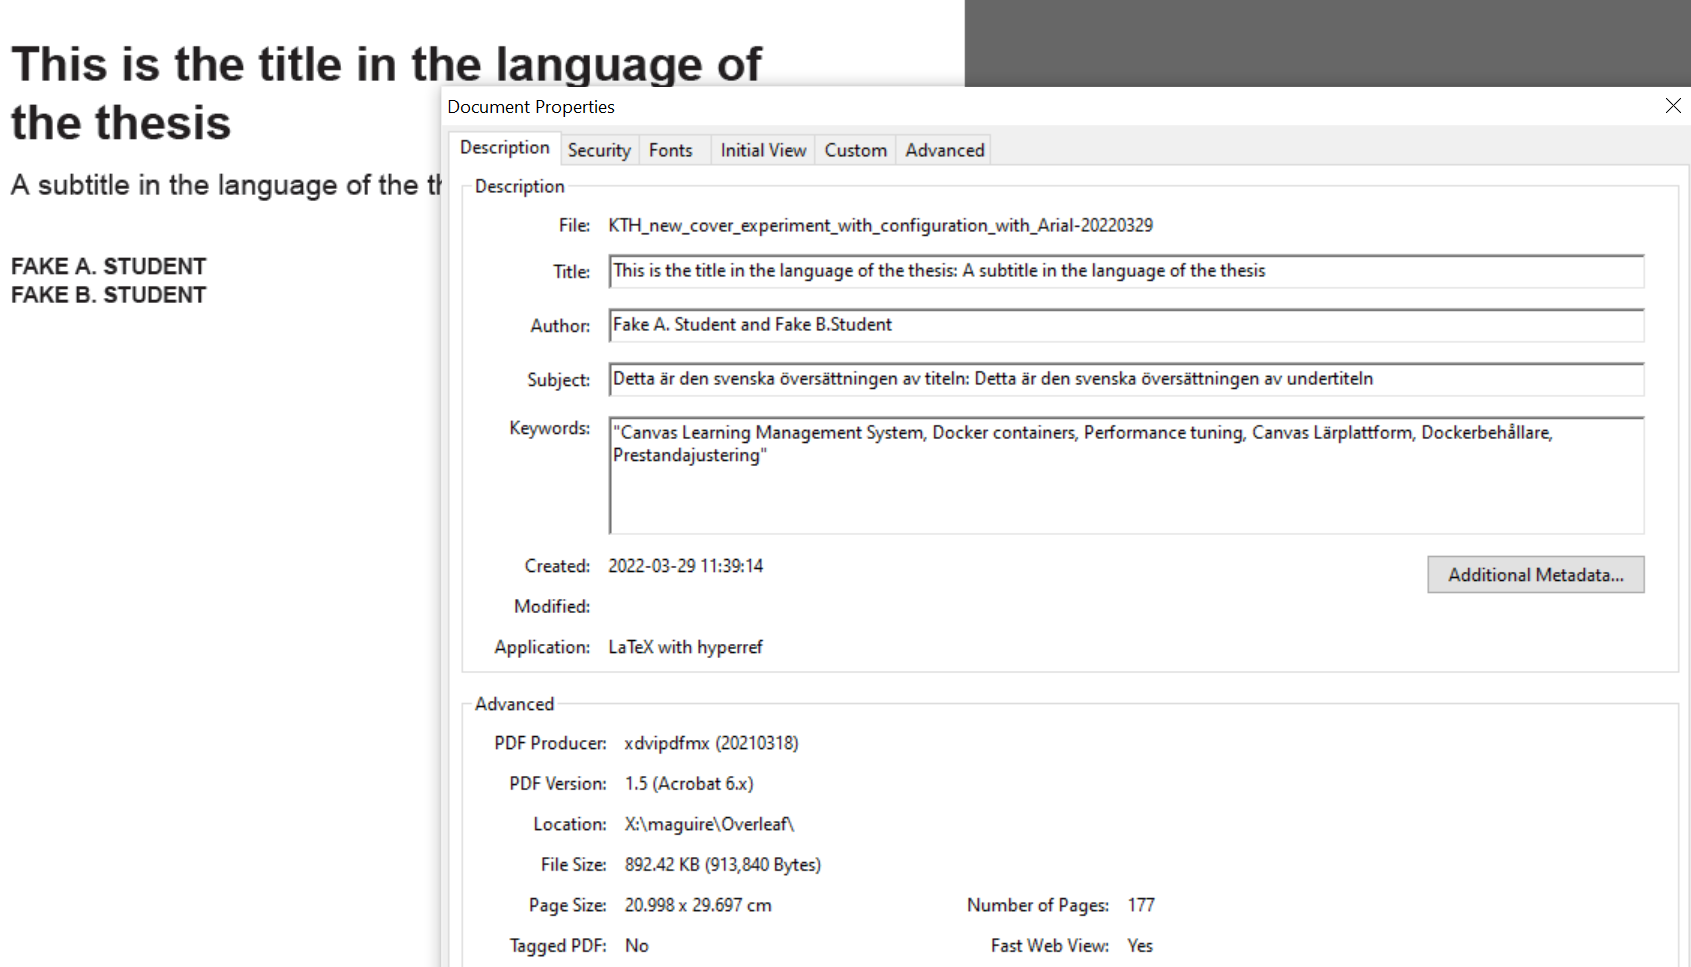
\includegraphics[width=1\textwidth]{README_notes/README-examiner-figures/PDF-file-metadata-Screenshot_20220330_085854.png}}
  \end{center}
  \caption{The title page of the thesis and the PDF metadata}
  \label{fig:pdfMetadata}
\end{figure}
\FloatBarrier	
\Needspace*{7\baselineskip}
\begin{lstlisting}[language={[LaTeX]TeX}, caption={The keywords appear as expected in the For DiVA data at the end of the PDF file}, label=lst:keywordsFromForDIVA]	
”Keywords[eng ]”: €€€€
Canvas Learning Management System, Docker containers, Performance tuning €€€€,

”Keywords[swe ]”: €€€€
Canvas Lärplattform, Dockerbehållare, Prestandajustering €€€€,
\end{lstlisting}

\section{Other variants of the JSON\_to\_calendar.py}
\label{sec:otherVariantsofJSONtoCalendar}
For testing purposes, I also created functionality in \texttt{JSON\_to\_calendar.py} to insert a fixed event (this was my first test) and to take as input a MODS file. The MODS file was created from a DiVA feed of theses presented in 2020 through to the 25\textsuperscript{th} of April. However, one limitation that I found is that other than myself, few people have been entering the date and time for the oral presentation. Unfortunately, since I wanted to test making calendar announcements, I needed data and time!

\Needspace*{2\baselineskip}
\textbf{NB}: I have assumed that each degree project presentation lasts one hour – since the KTH Cortina calendar API needs both a starting and ending time.

These other variants probably should not be kept, but rather the architecture should be similar to that shown in \Cref{fig:severalPossibleInputs}. Additionally, when taking data from other types of sources, one can take advantage of the data that is in a Canvas degree project course room to help when processing of the source data.

\begin{figure}[!ht]
\resizebox{\textwidth}{!}{%
\begin{tikzpicture}
[align=left,node distance=2cm]


\node (latexFile) [tape,tape bend top=none,draw,font=\sffamily] {\LaTeX file};
\node (PDFfile) [tape,tape bend top=none,draw,font=\sffamily, above of=latexFile] {PDF file};
\node (DOCXFile) [tape,tape bend top=none,draw,font=\sffamily, below of=latexFile] {DOCX file};

\node (extractor) [processBox, right=1cm of latexFile] {Extractor};
\node (jsonFile) [tape,tape bend top=none,draw,font=\sffamily, right=0.5cm of extractor] {JSON file};
\node (start) [processBox, right=0.5cm of jsonFile] {JSON\_to\_calendar};
\node (MODSFile) [tape,tape bend top=none,draw,font=\sffamily, above of=jsonFile] {MODS file};

\node (calendarEvent) [destinationBox, right=1cm of start] {Canvas calendar event};
\node (announcement) [destinationBox,  above of =calendarEvent] {Canvas announcement};
\node (cortinaCalendarEvent) [destinationBox,  right=0.5cm of start, below of=calendarEvent] {KTH Cortina calendar event};
\draw [arrow] (latexFile) --  (extractor.west);
\draw [arrow] (PDFfile) --  (extractor.west);
\draw [arrow] (DOCXFile) --  (extractor.west);
\draw [arrow] (extractor) --  (jsonFile.west);
\draw [arrow] (jsonFile) --  (start.west);
\draw [arrow] (start.east) --  (announcement.west);
\draw [arrow] (start.east) -- (calendarEvent);
\draw [arrow] (start.east) -- (cortinaCalendarEvent.west);
\draw [arrow, dashed] (MODSFile) --  node[right] {only for testing} (start.west);
\end{tikzpicture}
}
\caption{Several possible inputs to JSON\_to\_calendar.py  and its outputs}
  \label{fig:severalPossibleInputs}
\end{figure}




\section{JSON to MODS file}
\label{sec:JSONtoMODSfile}
In keeping with the idea of using the JSON file to drive other applications, the program JSON\_to\_MODS.py to creates a MODS file using the information from the arguments and a JSON file.
The program is patterned after the \texttt{JSON\_to\_calendar} and \texttt{JSON\_to\_cover} programs. The program outputs a MODS file called: \texttt{modsXML.xml}. The program is run as shown in \Cref{lst:jsonToMods}.
\Needspace*{5\baselineskip}
\begin{lstlisting}[language={bash}, caption={Example of using JSON\_to\_MODS.py}, label=lst:jsonToMods]
./JSON_to_MODS.py -c 11   --json test12.json --trita "TRITA-EECS-EX-2021:219" --testing
\end{lstlisting}


Note that currently the Canvas course information is not used. Note also that the “—testing” flag forces the report series to be  "TRITA-ICT-EX" overriding the actual series in in the input version of the DiVA data.

If acronyms are used in the abstracts, you can also add the “- -acronyms acronyms.tex” argument to the command line and the program will process the acronyms.

As noted above, you will get a file named \texttt{modsXML.xml} that you can manually import into DiVA. This process is shown in \Cref{sec:importingMODSfiletoDiVA}. I seem to be able to import these files into the test instance of DiVA:	\url{https://kth.test.diva-portal.org/dream/import/importList.jsf}. Another side-effect of the testing flag is to use the test instance of DiVA. \textbf{NB}: The organization units are different between the production and test version of DiVA. When run without the testing flag set, the MODS file can be imported into the production version of DiVA.

This program has been extended to be able to take the TRITA number information from the MODS file.


\subsection{Example of JSON to MODS}
The process of importing the MODS data into DiVA begins with the extracted JSON file (note that I have changed some of the formatting of the pseudo JSON information and added the export of the program code). An example of the JSON information is shown in \Cref{lst:test12.json}. The resulting MODS file is shown in \Cref{lst:test12.mods}.

\begin{lstlisting}[language={json}, caption={test12.json (manually reformatted)}, label=lst:test12.json]
{"Author1": {"Last name": "Student", "First name": "Fake A.", "Local User Id": "u100001", "E-mail": "a@kth.se", "organisation": {"L1": "School of XXX"}}, 
"Author2": {"Last name": "Student", "First name": "Fake B.", "Local User Id": "u100002", "E-mail": "b@kth.se", "organisation": {"L1": "School of XXX"}}, 
"Degree": {"Educational program": "Bachelor’s Programme in XXX", "programcode": "TCOMK", "Level": "1", "Course code": "XX100X", "Credits": "15.0", "Exam": "Bachelors degree", "subjectArea": "subject area"},
"Title": {"Main title": "This is the title in the language of the thesis", "Subtitle": "An subtitle in the language of the thesis", "Language": "eng"},
"Alternative title": {"Main title": "Detta är den svenska översättningen av titeln", "Subtitle": "Detta är den svenska översättningen av undertiteln", "Language": "swe"},
"Supervisor1": {"Last name": "Supervisor", "First name": "A. Busy", "Local User Id": "u100003", "E-mail": "sa@kth.se", "organisation": {"L1": "School of XXX", "L2": "DepartmentName"}},
"Supervisor2": {"Last name": "Supervisor", "First name": "Another Busy", "Local User Id": "u100003", "E-mail": "sb@kth.se", "organisation": {"L1": "School of XXX", "L2": "DepartmentName"}}, 
"Supervisor3": {"Last name": "Supervisor", "First name": "Third Busy", "E-mail": "sc@tu.va", "Other organisation": "Timbuktu University, Department of Pseudoscience"},
"Examiner1": {"Last name": "ExaminersLastname", "First name": "ExaminersFirstname", "Local User Id": "u1000000", "E-mail": "xxx@kth.se", "organisation": {"L1": "School of XXX", "L2": "DepartmentName"}},
"Cooperation": {"Partner_name": "Företaget AB"}, "National Subject Categories": "10201, 10206", "Other information": {"Year": "2021", "Number of pages": "xxxiii,35"}, "Opponents": {"Name": "A. B. Normal & A. X. E. Normalè"}, "Presentation": {"Date": "2021-03-15 13:00", "Language": "eng", "Room": "via Zoom https://kth-se.zoom.us/j/ddddddddddd", "Address": "Isafjordsgatan 22 (Kistagången 16)", "City": "Stockholm"},
"Number of lang instances": "10", "abstracts": {"eng": "<p>All theses at KTH are <bold>required</bold> to have an abstract in both <i>English</i> and <i>Swedish</i>.</p><p>Exchange students many want to include one or more abstracts in the language(s) used in their home institutions to avoid the need to write another thesis when returning to their home institution.</p><p>Keep in mind that most of your potential readers are only going to read your <tt>title</tt> and <tt>abstract</tt>. This is why it is important that the abstract give them enough information that they can decide is this document relevant to them or not. Otherwise the likely default choice is to ignore the rest of your document.</p><p>A abstract should stand on its own, i.e., no citations, cross references to the body of the document, acronyms must be spelled out, … .</p><p>Write this early and revise as necessary. This will help keep you focused on what you are trying to do.</p><p>Write an abstract with the following components: </p><ul><li> What is the topic area? (optional) Introduces the subject area for the project. </li><li> Short problem statement </li><li> Why was this problem worth a Bachelor’s/’Masters thesis project? (i.e., why is the problem both significant and of a suitable degree of difficulty for a Bachelor’s/’Masters thesis project? Why has no one else solved it yet?) </li><li> How did you solve the problem? What was your method/insight? </li><li> Results/Conclusions/Consequences/Impact: What are your key results/conclusions? What will others do based upon your results? What can be done now that you have finished - that could not be done before your thesis project was completed?</li></ul><p>announcement of the oral presentation and for entering data into DiVA</p><p>\\pi \\cdot r$ or \\[ \\int_{a}^{b} x^2 \\,dx \\]</p><p></p><p> A<sup>*</sup>, A<sup>&reg;</sup>, and A&trade;.</p><p> first chemical formula can be handled, while the second will require hand editing</p>",
"swe": "<p>Alla avhandlingar vid KTH <bold>måste ha</bold> ett abstrakt på både <i>engelska</i> och <i>svenska</i>.</p><p>Om du skriver din avhandling på svenska ska detta göras först (och placera det som det första abstraktet) - och du bör revidera det vid behov.</p><p>If you are writing your thesis in English, you can leave this until the draft version that goes to your opponent for the written opposition. In this way you can provide the English and Swedish abstract/summary information that can be used in the announcement for your oral presentation.</p><p>If you are writing your thesis in English, then this section can be a summary targeted at a more general reader. However, if you are writing your thesis in Swedish, then the reverse is true – your abstract should be for your target audience, while an English summary can be written targeted at a more general audience.</p><p>This means that the English abstract and Swedish sammnfattning or Swedish abstract and English summary need not be literal translations of each other.</p><p>The abstract in the language used for the thesis should be the first abstract, while the Summary/Sammanfattning in the other language can follow.</p>",
"fre": "<p>Résumé en français.</p>", "spa": "<p>Résumé en espagnol.</p>", "ita": "<p>Sommario in italiano.</p>",
"nor": "<p>Sammendrag på norsk.</p>", "ger": "", "dan": "<p>Abstrakt på dansk.</p>",
"dut": "<p>Zusammenfassung in Deutsch.</p><p>Samenvatting in het Nederlands.</p><p>Eesti keeles kokkuvõte.</p>", "est": ""},
"keywords": {"eng": "Canvas Learning Management System, Docker containers, Performance tuning ",
"swe": "Canvas Lärplattform, Dockerbehållare, Prestandajustering\nNyckelord som beskriver innehållet i uppsatsrapporten\n",
"fre": "5-6 mots-clés ", "spa": "5-6 Palabras claves ", "ita": "5-6 parole chiave ",
"nor": "5-6 nøkkelord ", "ger": "5-6 Schlüsselwörter ", "dan": "5-6 Søgeord ",
"dut": "5-6 trefwoorden ", "est": "5-6 Märksõnad "}}
\end{lstlisting}

\clearpage

\begin{lstlisting}[language={XML}, caption={test12.mods (reformatted in EMACS using XML mode)}, label=lst:test12.mods]
<modsCollection xmlns="http://www.loc.gov/mods/v3" xmlns:xsi="http://www.w3.org/2001/XMLSchema-instance" xsi:schemaLocation="http://www.loc.gov/mods/v3 http://www.loc.gov/standards/mods/v3/mods-3-2.xsd">
  <mods xmlns="http://www.loc.gov/mods/v3" xmlns:xsi="http://www.w3.org/2001/XMLSchema-instance" xmlns:xlink="http://www.w3.org/1999/xlink" version="3.2" xsi:schemaLocation="http://www.loc.gov/mods/v3 http://www.loc.gov/standards/mods/v3/mods-3-2.xsd">
    <genre authority="diva" type="publicationTypeCode">studentThesis
    </genre>
    <genre authority="diva" type="publicationType" lang="swe">Studentuppsats (Examensarbete)
    </genre>
    <genre authority="diva" type="publicationType" lang="eng">Student thesis
    </genre>
    <genre authority="diva" type="publicationType" lang="nor">Oppgave
    </genre>
    <name type="personal" authority="kth" xlink:href="u100001">
      <namePart type="family">Student
      </namePart>
      <namePart type="given">Fake A.
      </namePart>
      <description>email=a@kth.se
      </description>
      <role>
	<roleTerm type="code" authority="marcrelator">aut
	</roleTerm>
      </role>
    </name>
    <name type="personal" authority="kth" xlink:href="u100002">
      <namePart type="family">Student
      </namePart>
      <namePart type="given">Fake B.
      </namePart>
      <description>email=b@kth.se
      </description>
      <role>
	<roleTerm type="code" authority="marcrelator">aut
	</roleTerm>
      </role>
    </name>
    <name type="personal" authority="kth" xlink:href="u1d13i2c">
      <namePart type="family">Maguire Jr.
      </namePart>
      <namePart type="given">Gerald Q.
      </namePart>
      <description>email=maguire@kth.se
      </description>
      <affiliation>KTH, School of XXX, DepartmentName
      </affiliation>
      <role>
	<roleTerm type="code" authority="marcrelator">mon
	</roleTerm>
      </role>
    </name>
    <name type="personal" authority="kth" xlink:href="u100003">
      <namePart type="family">Supervisor
      </namePart>
      <namePart type="given">A. Busy
      </namePart>
      <affiliation>School of School of XXX, DepartmentName
      </affiliation>
      <description>email=sa@kth.se
      </description>
      <role>
	<roleTerm type="code" authority="marcrelator">ths
	</roleTerm>
      </role>
    </name>
    <name type="personal" authority="kth" xlink:href="u100003">
      <namePart type="family">Supervisor
      </namePart>
      <namePart type="given">Another Busy
      </namePart>
      <affiliation>School of School of XXX, DepartmentName
      </affiliation>
      <description>email=sb@kth.se
      </description>
      <role>
	<roleTerm type="code" authority="marcrelator">ths
	</roleTerm>
      </role>
    </name>
    <name type="personal">
      <namePart type="family">Supervisor
      </namePart>
      <namePart type="given">Third Busy
      </namePart>
      <affiliation>Timbuktu University, Department of Pseudoscience
      </affiliation>
      <description>email=sc@tu.va
      </description>
      <role>
	<roleTerm type="code" authority="marcrelator">ths
	</roleTerm>
      </role>
    </name>
    <name>
      <namePart>KTH
      </namePart>
      <namePart> School of XXX
      </namePart>
      <namePart> DepartmentName
      </namePart>
      <role>
	<roleTerm type="code" authority="marcrelator">pbl
	</roleTerm>
      </role>
    </name>
    <titleInfo  lang="eng">
      <title>This is the title in the language of the thesis
      </title>
      <subTitle>An subtitle in the language of the thesis
      </subTitle>
    </titleInfo >
    <titleInfo  lang="swe" type="alternative">
      <title>Detta är den svenska översättningen av titeln
      </title>
      <subTitle>Detta är den svenska översättningen av undertiteln
      </subTitle>
    </titleInfo >
    <subject  lang="eng">
      <topic>Canvas Learning Management System
      </topic>
      <topic>Docker containers
      </topic>
      <topic>Performance tuning
      </topic>
    </subject >
    <subject  lang="swe">
      <topic>Canvas Lärplattform
      </topic>
      <topic>Dockerbehållare
      </topic>
      <topic>Prestandajustering Nyckelord som beskriver innehållet i uppsatsrapporten
      </topic>
    </subject >
    <subject  lang="fre">
      <topic>5-6 mots-clés
      </topic>
    </subject >
    <subject  lang="spa">
      <topic>5-6 Palabras claves
      </topic>
    </subject >
    <subject  lang="ita">
      <topic>5-6 parole chiave
      </topic>
    </subject >
    <subject  lang="nor">
      <topic>5-6 nøkkelord
      </topic>
    </subject >
    <subject  lang="ger">
      <topic>5-6 Schlüsselwörter
      </topic>
    </subject >
    <subject  lang="dan">
      <topic>5-6 Søgeord
      </topic>
    </subject >
    <subject  lang="dut">
      <topic>5-6 trefwoorden
      </topic>
    </subject >
    <subject  lang="est">
      <topic>5-6 Märksõnad
      </topic>
    </subject >
    <abstract  lang="eng">&lt;p&gt;All theses at KTH are &lt;bold&gt;required&lt;/bold&gt; to have an abstract in both &lt;i&gt;English&lt;/i&gt; and &lt;i&gt;Swedish&lt;/i&gt;.&lt;/p&gt;&lt;p&gt;Exchange students many want to include one or more abstracts in the language(s) used in their home institutions to avoid the need to write another thesis when returning to their home institution.&lt;/p&gt;&lt;p&gt;Keep in mind that most of your potential readers are only going to read your &lt;tt&gt;title&lt;/tt&gt; and &lt;tt&gt;abstract&lt;/tt&gt;. This is why it is important that the abstract give them enough information that they can decide is this document relevant to them or not. Otherwise the likely default choice is to ignore the rest of your document.&lt;/p&gt;&lt;p&gt;A abstract should stand on its own, i.e., no citations, cross references to the body of the document, acronyms must be spelled out, … .&lt;/p&gt;&lt;p&gt;Write this early and revise as necessary. This will help keep you focused on what you are trying to do.&lt;/p&gt;&lt;p&gt;Write an abstract with the following components: &lt;/p&gt;&lt;ul&gt;&lt;li&gt; What is the topic area? (optional) Introduces the subject area for the project. &lt;/li&gt;&lt;li&gt; Short problem statement &lt;/li&gt;&lt;li&gt; Why was this problem worth a Bachelor’s/’Masters thesis project? (i.e., why is the problem both significant and of a suitable degree of difficulty for a Bachelor’s/’Masters thesis project? Why has no one else solved it yet?) &lt;/li&gt;&lt;li&gt; How did you solve the problem? What was your method/insight? &lt;/li&gt;&lt;li&gt; Results/Conclusions/Consequences/Impact: What are your key results/conclusions? What will others do based upon your results? What can be done now that you have finished - that could not be done before your thesis project was completed?&lt;/li&gt;&lt;/ul&gt;&lt;p&gt;announcement of the oral presentation and for entering data into DiVA&lt;/p&gt;&lt;p&gt;\pi \cdot r$ or &lt;span class='math-tex'&gt;\[ \int_{a}^{b} x^2 \,dx \]&lt;/span&gt;&lt;/p&gt;&lt;p&gt;&lt;/p&gt;&lt;p&gt; A&lt;sup&gt;*&lt;/sup&gt;, A&lt;sup&gt;&amp;reg;&lt;/sup&gt;, and A&amp;trade;.&lt;/p&gt;&lt;p&gt; first chemical formula can be handled, while the second will require hand editing&lt;/p&gt;
    </abstract >
    <abstract  lang="swe">&lt;p&gt;Alla avhandlingar vid KTH &lt;bold&gt;måste ha&lt;/bold&gt; ett abstrakt på både &lt;i&gt;engelska&lt;/i&gt; och &lt;i&gt;svenska&lt;/i&gt;.&lt;/p&gt;&lt;p&gt;Om du skriver din avhandling på svenska ska detta göras först (och placera det som det första abstraktet) - och du bör revidera det vid behov.&lt;/p&gt;&lt;p&gt;If you are writing your thesis in English, you can leave this until the draft version that goes to your opponent for the written opposition. In this way you can provide the English and Swedish abstract/summary information that can be used in the announcement for your oral presentation.&lt;/p&gt;&lt;p&gt;If you are writing your thesis in English, then this section can be a summary targeted at a more general reader. However, if you are writing your thesis in Swedish, then the reverse is true – your abstract should be for your target audience, while an English summary can be written targeted at a more general audience.&lt;/p&gt;&lt;p&gt;This means that the English abstract and Swedish sammnfattning or Swedish abstract and English summary need not be literal translations of each other.&lt;/p&gt;&lt;p&gt;The abstract in the language used for the thesis should be the first abstract, while the Summary/Sammanfattning in the other language can follow.&lt;/p&gt;
    </abstract >
    <abstract  lang="fre">&lt;p&gt;Résumé en français.&lt;/p&gt;
    </abstract >
    <abstract  lang="spa">&lt;p&gt;Résumé en espagnol.&lt;/p&gt;
    </abstract >
    <abstract  lang="ita">&lt;p&gt;Sommario in italiano.&lt;/p&gt;
    </abstract >
    <abstract  lang="nor">&lt;p&gt;Sammendrag på norsk.&lt;/p&gt;
    </abstract >
    <abstract  lang="ger" />
    <abstract  lang="dan">&lt;p&gt;Abstrakt på dansk.&lt;/p&gt;
    </abstract >
    <abstract  lang="dut">&lt;p&gt;Zusammenfassung in Deutsch.&lt;/p&gt;&lt;p&gt;Samenvatting in het Nederlands.&lt;/p&gt;&lt;p&gt;Eesti keeles kokkuvõte.&lt;/p&gt;
    </abstract >
    <abstract  lang="est" />
    <physicalDescription>
      <form authority="marcform">electronic
      </form>
      <extent>xxxiii,35
      </extent>
    </physicalDescription>
    <originInfo>
      <place>
	<placeTerm>Stockholm
	</placeTerm>
      </place>
      <publisher>KTH Royal Institute of Technology
      </publisher>
      <dateIssued>2021
      </dateIssued>
      <dateOther type="defence">2021-03-15T13:00:00
      </dateOther>
    </originInfo>
    <typeOfResource>text
    </typeOfResource>
    <relatedItem  type="series">
      <titleInfo>
	<title>TRITA-ICT-EX
	</title>
	<identifier type="local">5952
	</identifier>
	<identifier type="issue number">2021:219
	</identifier>
      </titleInfo>
    </relatedItem >
    <note lang="swe" type="level">Självständigt arbete på grundnivå (kandidatexamen)
    </note>
    <note lang="eng" type="degree">Bachelors degree
    </note>
    <note lang="swe" type="universityCredits">10 poäng / 15 hp
    </note>
    <subject lang="swe" xlink:href="10329">
      <topic>Informations- och kommunikationsteknik
      </topic>
      <genre>Subject/course
      </genre>
    </subject>
    <subject lang="eng" xlink:href="10329">
      <topic>Information and Communication Technology
      </topic>
      <genre>Subject/course
      </genre>
    </subject>
    <subject lang="swe" xlink:href="9925">
      <topic>Teknologie kandidatexamen - Informations- och kommunikationsteknik
      </topic>
      <genre>Educational program
      </genre>
    </subject>
    <subject lang="eng" xlink:href="9925">
      <topic>Bachelor of Science - Information and Communication Technology
      </topic>
      <genre>Educational program
      </genre>
    </subject>
    <language objectPart="defence">
      <languageTerm type="code" authority="iso639-2b">eng
      </languageTerm>
    </language>
    <note type="venue">via Zoom https://kth-se.zoom.us/j/ddddddddddd,Isafjordsgatan 22 (Kistagången 16),Stockholm
    </note>
    <note type="cooperation">Företaget AB
    </note>
    <subject lang="eng" authority="hsv" xlink:href="10201">
      <topic>Natural Sciences
      </topic>
      <topic>Computer and Information Sciences
      </topic>
      <topic>Computer Sciences
      </topic>
    </subject>
    <subject lang="swe" authority="hsv" xlink:href="10201">
      <topic>Naturvetenskap
      </topic>
      <topic>Data- och informationsvetenskap
      </topic>
      <topic>Datavetenskap (datalogi)
      </topic>
    </subject>
    <subject lang="eng" authority="hsv" xlink:href="10206">
      <topic>Natural Sciences
      </topic>
      <topic>Computer and Information Sciences
      </topic>
      <topic>Computer Engineering
      </topic>
    </subject>
    <subject lang="swe" authority="hsv" xlink:href="10206">
      <topic>Naturvetenskap
      </topic>
      <topic>Data- och informationsvetenskap
      </topic>
      <topic>Datorteknik
      </topic>
    </subject>
  </mods>
</modsCollection>
\end{lstlisting}
	
\subsection{Importing MODS file to DiVA}
\label{sec:importingMODSfiletoDiVA}

\Cref{fig:divaImport1} to \Cref{fig:divaImport4} show the process of importing the MODS file into DiVA. Note that it skips the first user interface form (as this differs between users).

\begin{figure}[!ht]
  \begin{center}
    \fbox{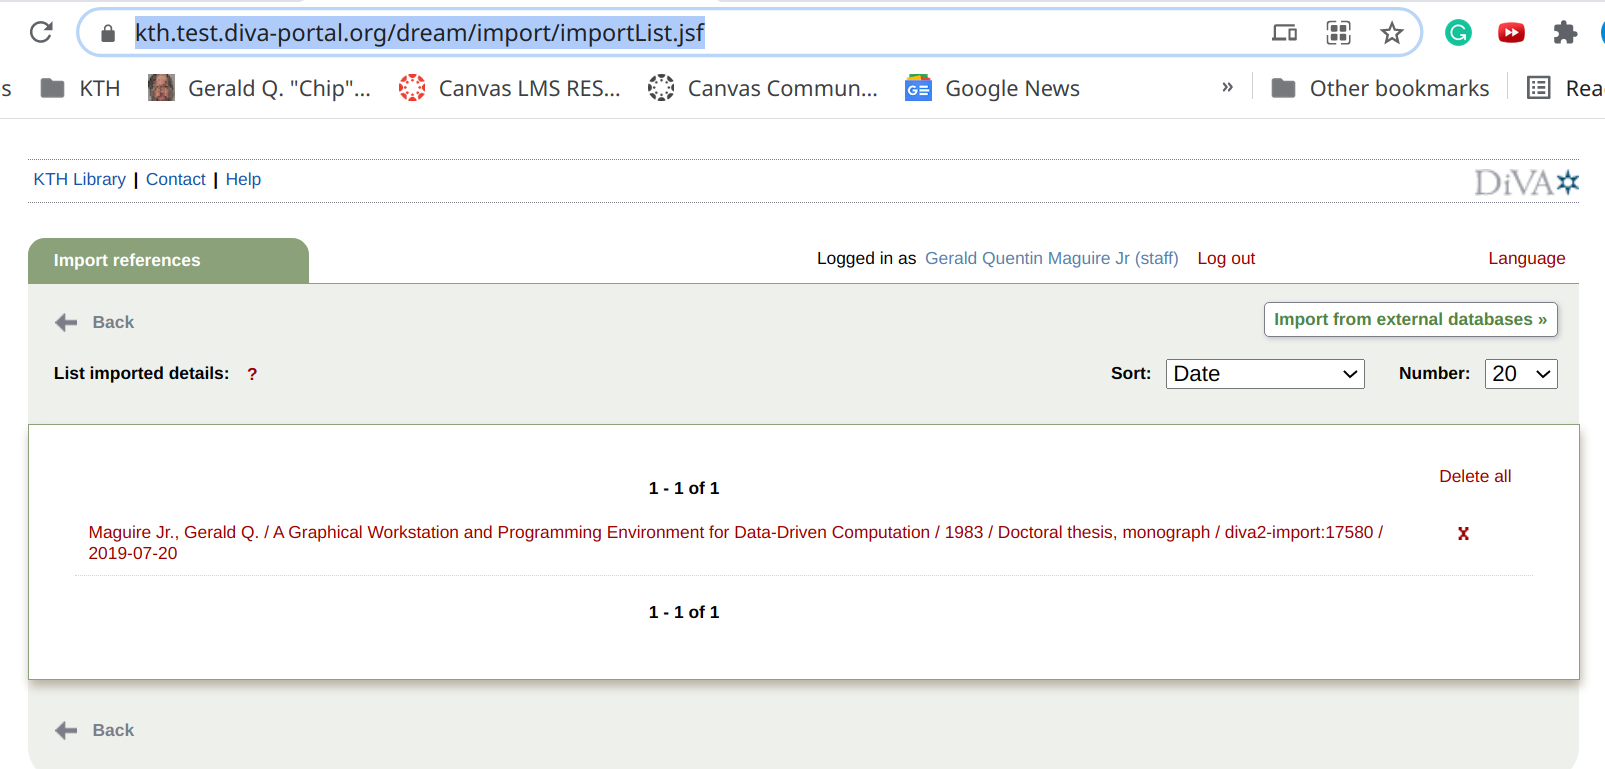
\includegraphics[width=1\textwidth]{README_notes/README-examiner-figures/import-1-Screenshot_20210626_234259.png}}
  \end{center}
  \caption[The import process – step 1]{The import process – step 1 – click on the “Import from external database” button on the upper right corner}
  \label{fig:divaImport1}
\end{figure}
\FloatBarrier

\begin{figure}[!ht]
  \begin{center}
    \fbox{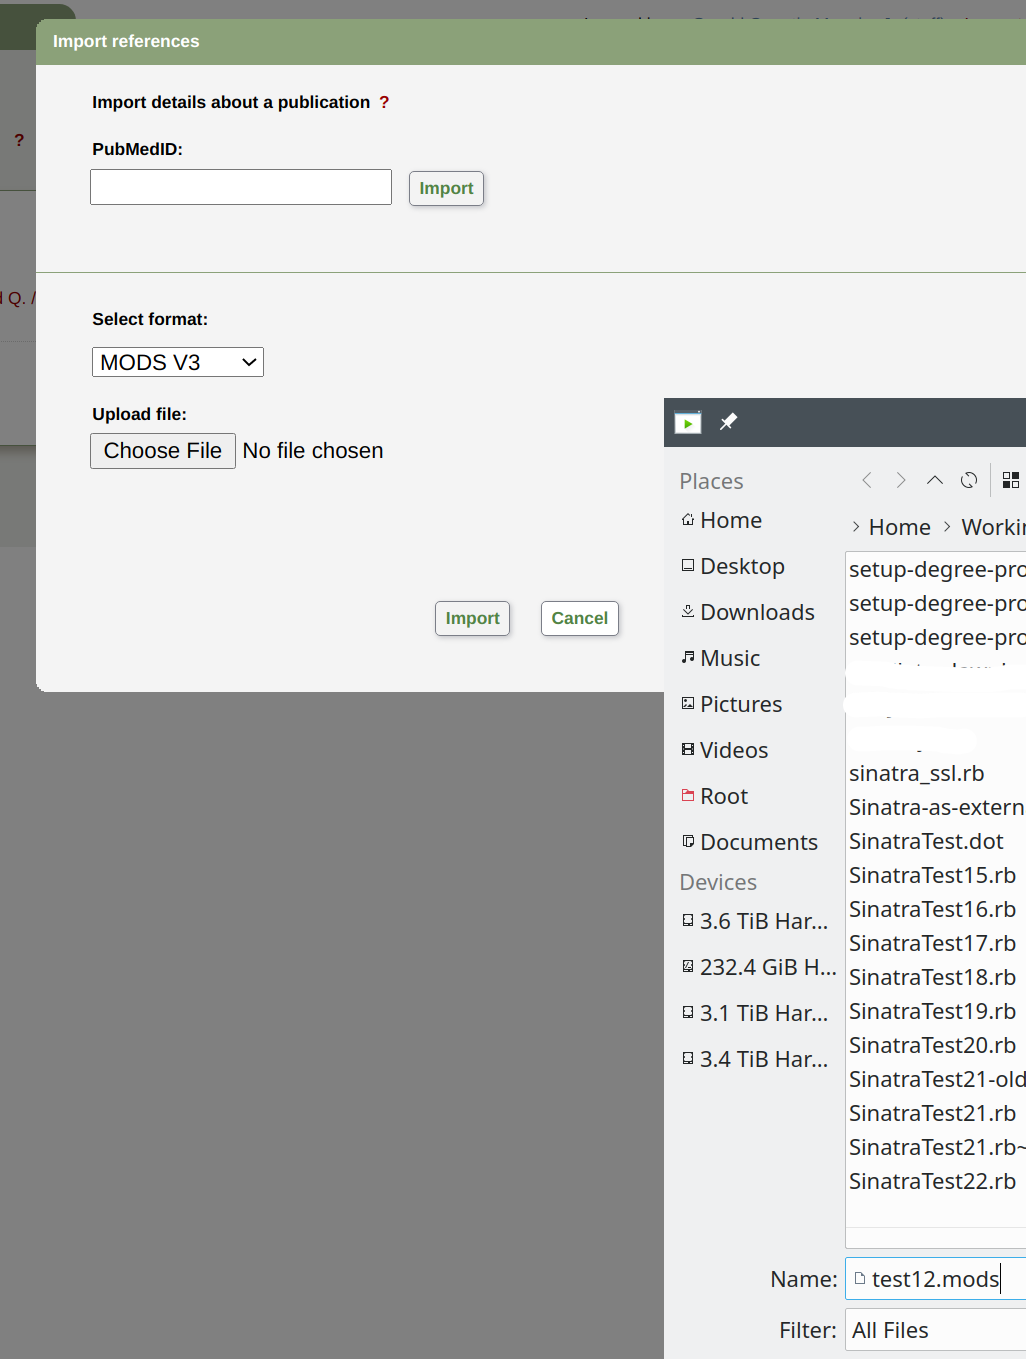
\includegraphics[width=1\textwidth]{README_notes/README-examiner-figures/import-2-Screenshot_20210626_234414.png}}
  \end{center}
  \caption[The import process – step 2]{The import process – step 2 – choose the MODV3 format and select a file to import}
  \label{fig:divaImport2}
\end{figure}
\FloatBarrier

\begin{figure}[!ht]
  \begin{center}
    \fbox{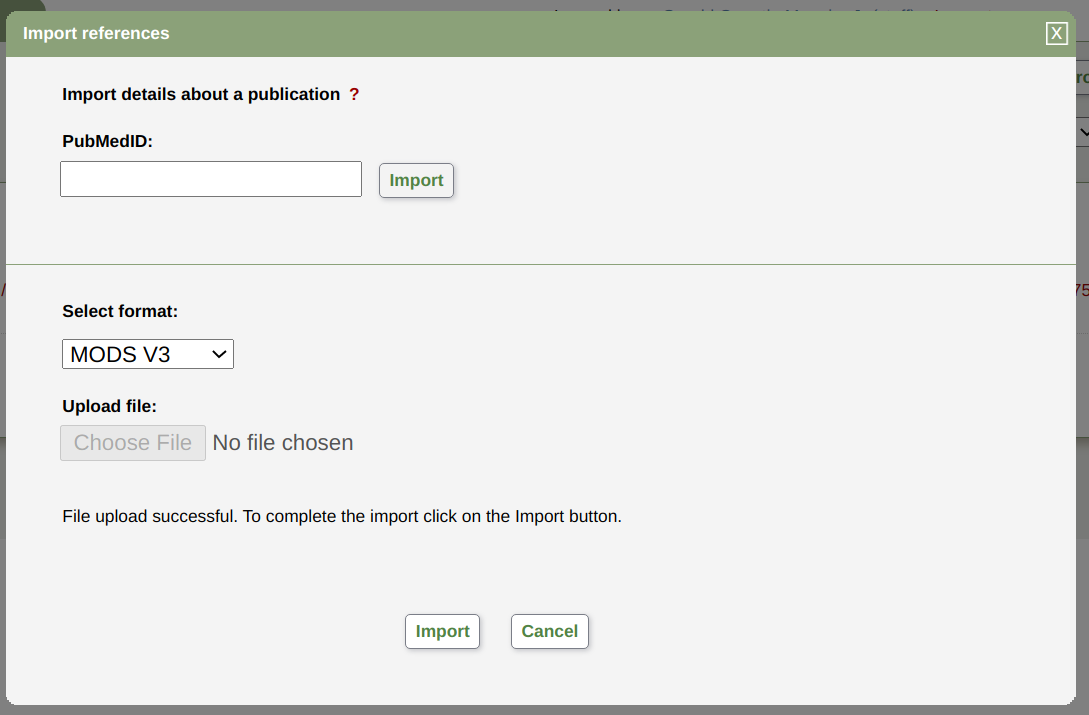
\includegraphics[width=1\textwidth]{README_notes/README-examiner-figures/import-3-Screenshot_20210626_234447.png}}
  \end{center}
  \caption[The import process – step 3]{The import process – step 3 – after clicking “Import” – it says that the file was successfully uploaded
Click on “Import” again to load the file. The MODS files is loaded and shown in \Cref{fig:divaImport4}.}
  \label{fig:divaImport3}
\end{figure}
\FloatBarrier

\begin{figure}[!ht]
  \begin{center}
    \fbox{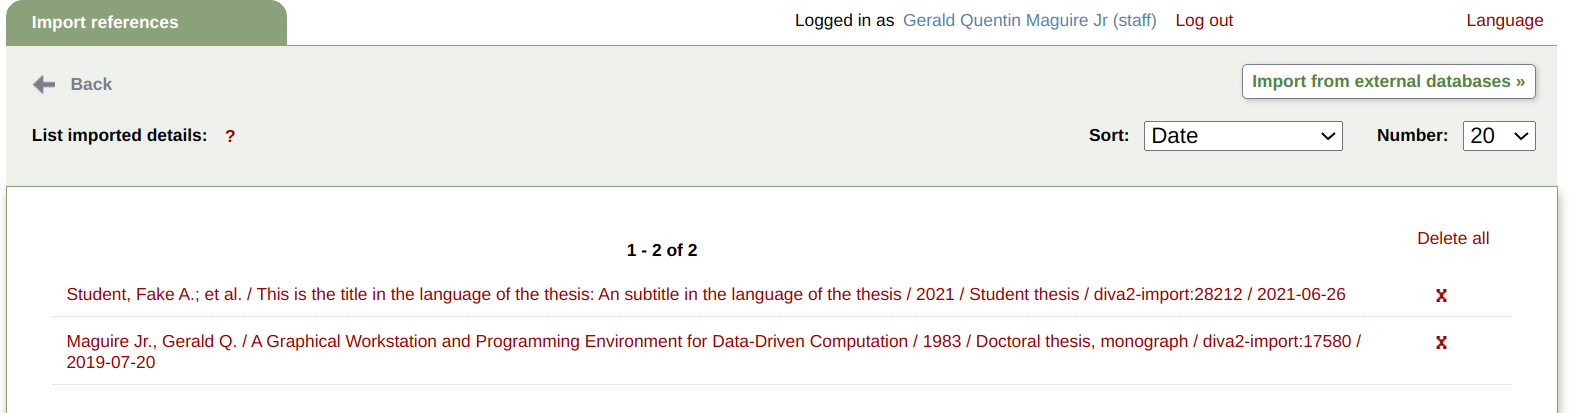
\includegraphics[width=1\textwidth]{README_notes/README-examiner-figures/import-4-Screenshot_20210626_234519.png}}
  \end{center}
  \caption[The import process – step 4]{The import process – step 4 – after clicking “Import” once more – you can see the file has been added to the list of imported files The imported document is shown in \Cref{fig:divaImport5} to \Cref{fig:divaImport12}.}
  \label{fig:divaImport4}
\end{figure}
\FloatBarrier

\begin{figure}[!ht]
  \begin{center}
    \fbox{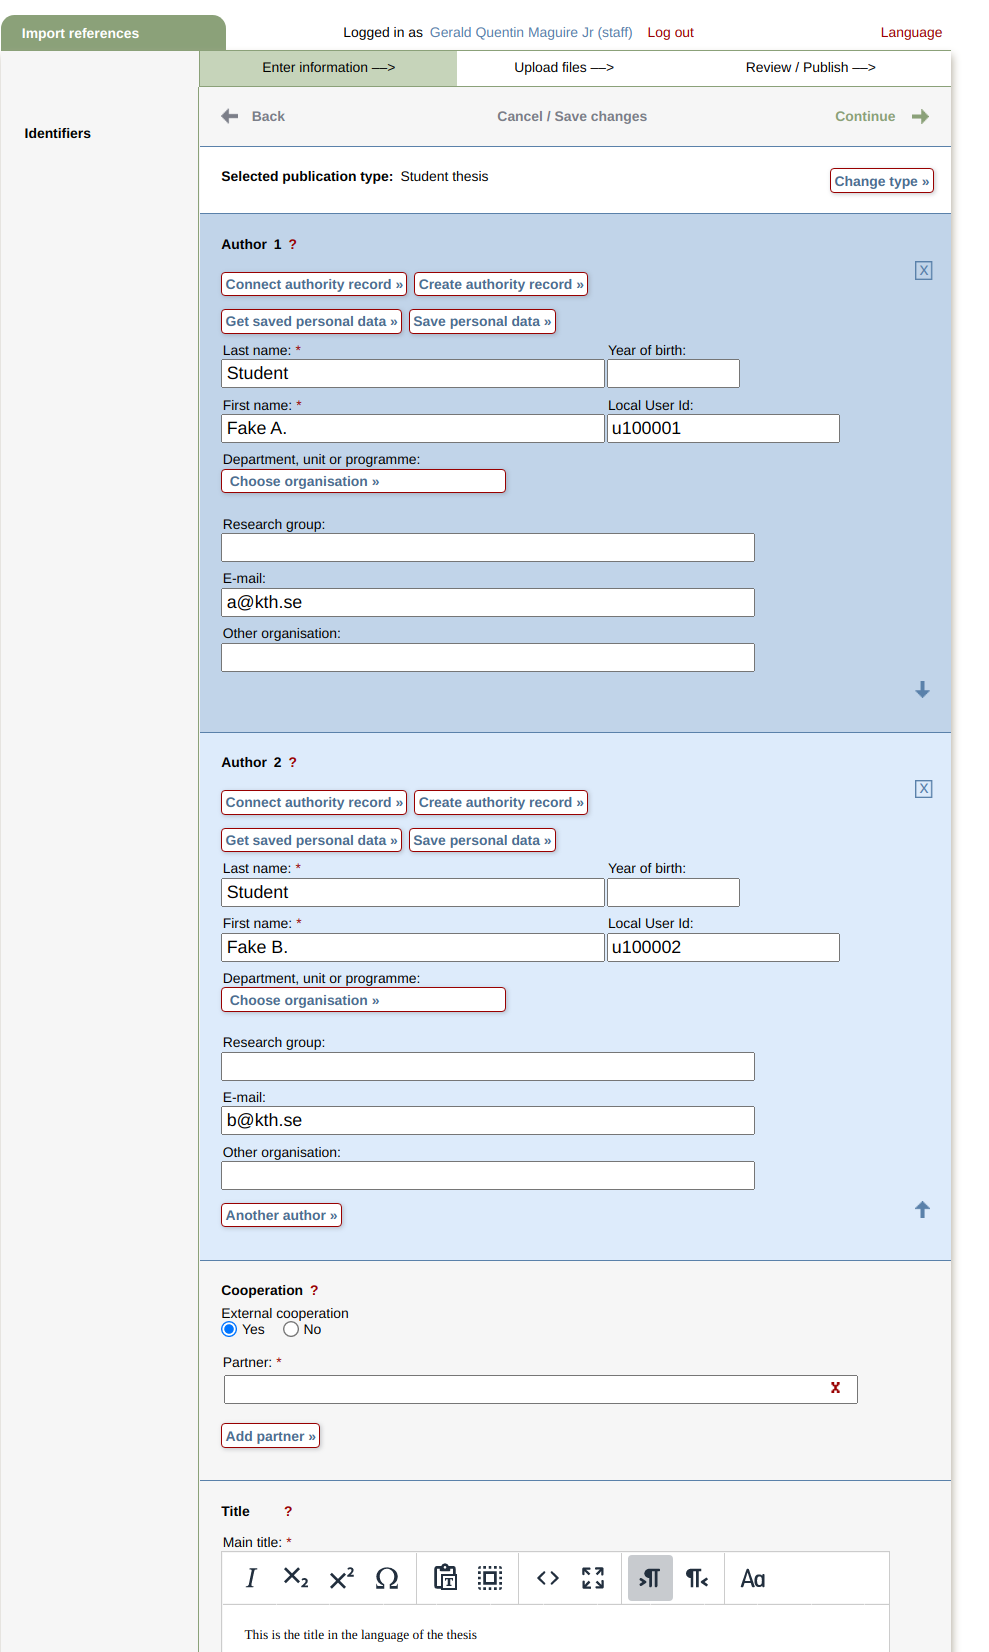
\includegraphics[width=0.8\textwidth]{README_notes/README-examiner-figures/import-a-Screenshot_20210626_234606.png}}
  \end{center}
  \caption[Imported document (part 1)]{Imported document (part 1)}
  \label{fig:divaImport5}
\end{figure}
\FloatBarrier

\begin{figure}[!ht]
  \begin{center}
    \fbox{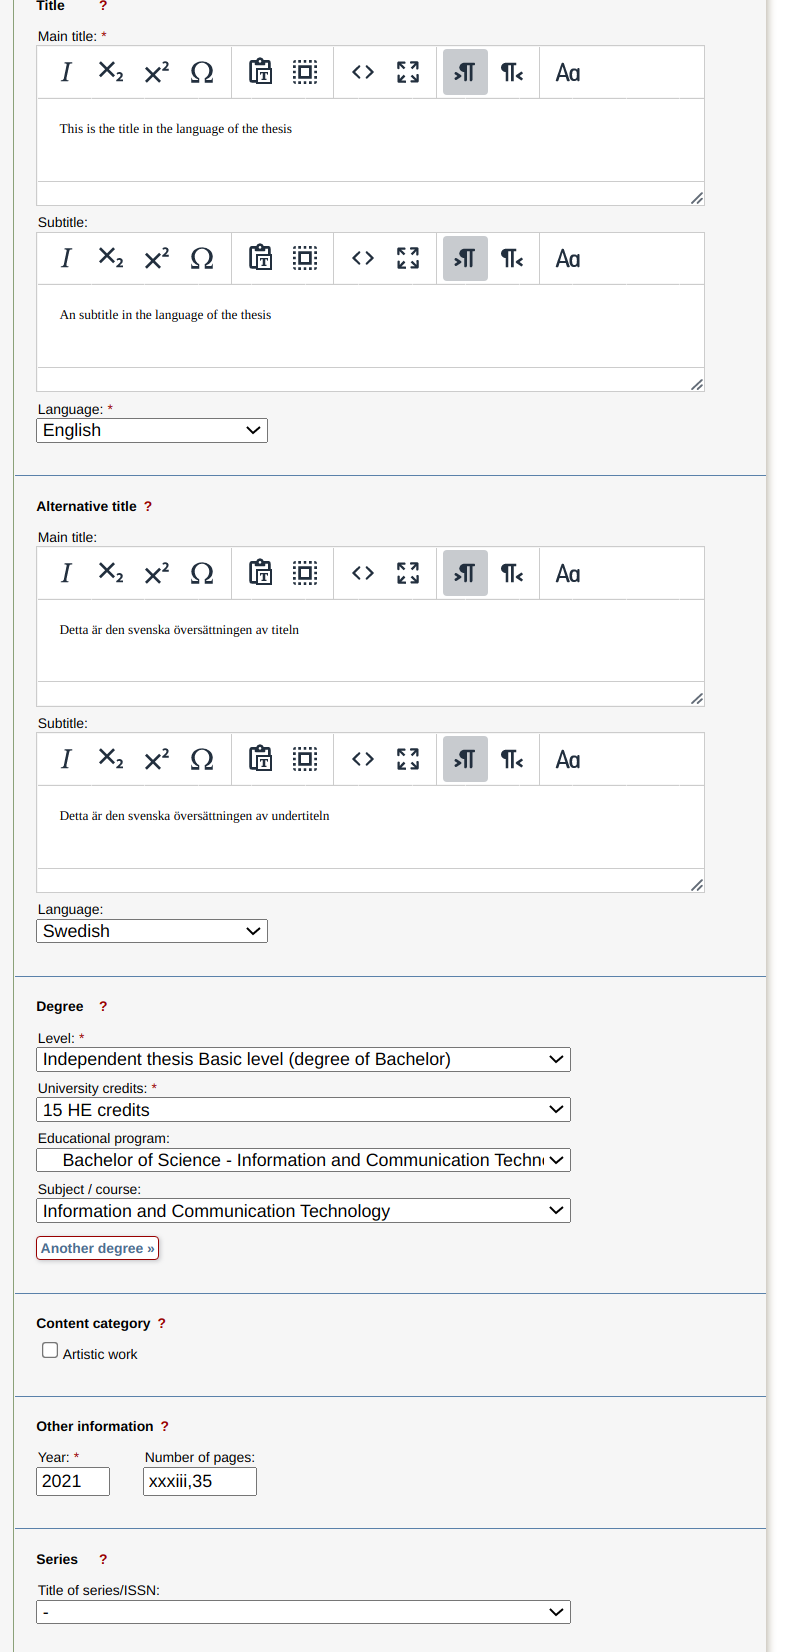
\includegraphics[width=0.65\textwidth]{README_notes/README-examiner-figures/import-b-Screenshot_20210626_234640.png}}
  \end{center}
  \caption[Imported document (part 2)]{Imported document (part 2) – Note that both the English and Swedish titles are shown as well as the information about which level, the number of university credits, the education al program, and the subject.- Additionally, the year and number of pages are shown.}
  \label{fig:divaImport6}
\end{figure}
\FloatBarrier

\begin{figure}[!ht]
  \begin{center}
    \fbox{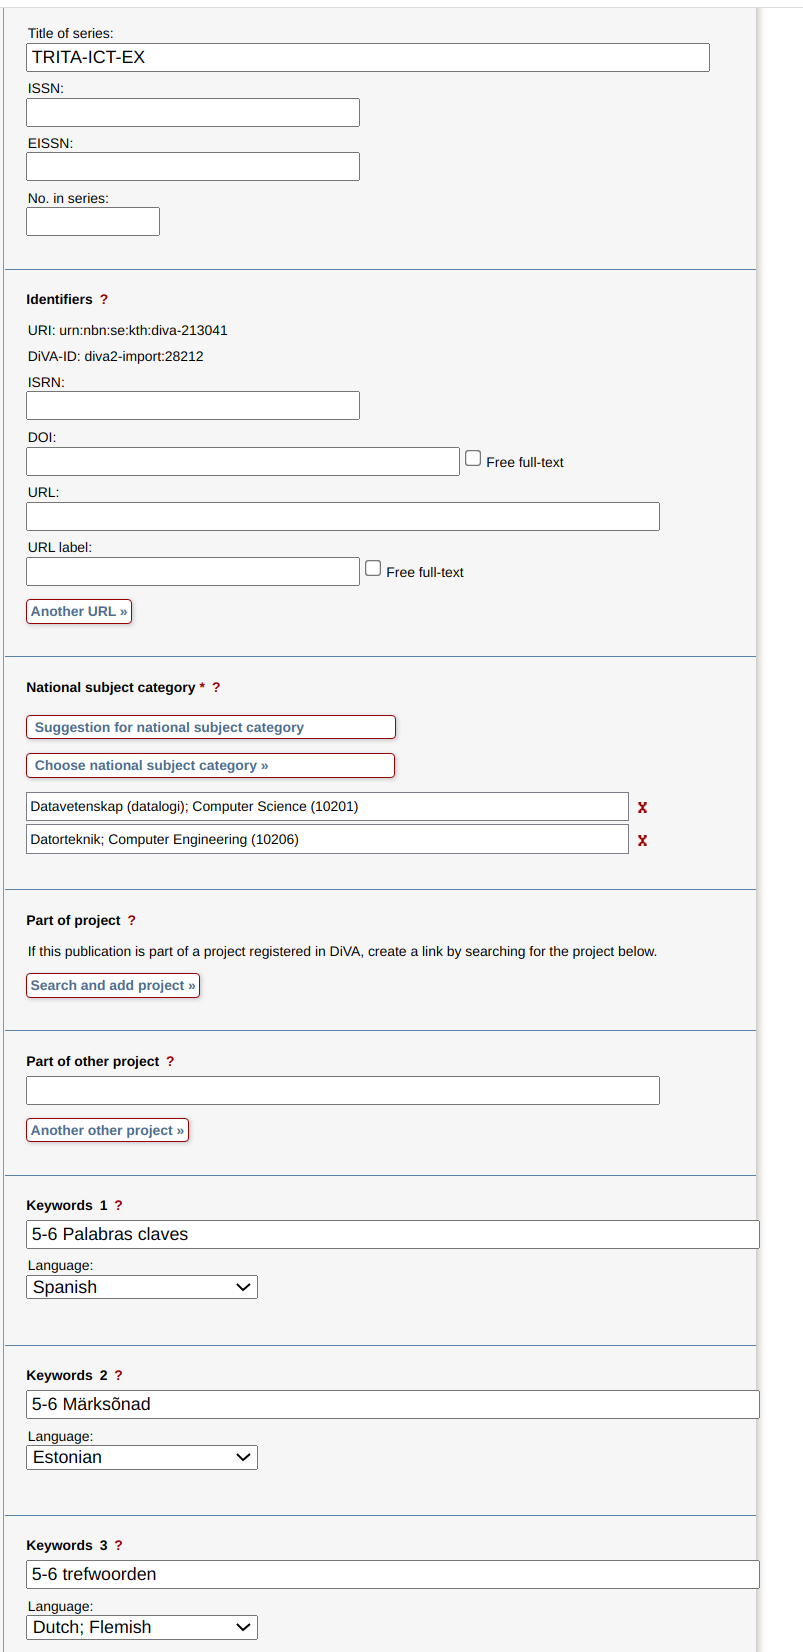
\includegraphics[width=0.65\textwidth]{README_notes/README-examiner-figures/import-c-Screenshot_20210626_234710.png}}
  \end{center}
  \caption[Imported document (part 3)]{Imported document (part 3) – Note that the number in the series is not being shown. The nation subject catergies specified in the JSON file are shown. Additionally, a number of the keyoards in different languages are shown.}
  \label{fig:divaImport7}
\end{figure}
\FloatBarrier

\begin{figure}[!ht]
  \begin{center}
    \fbox{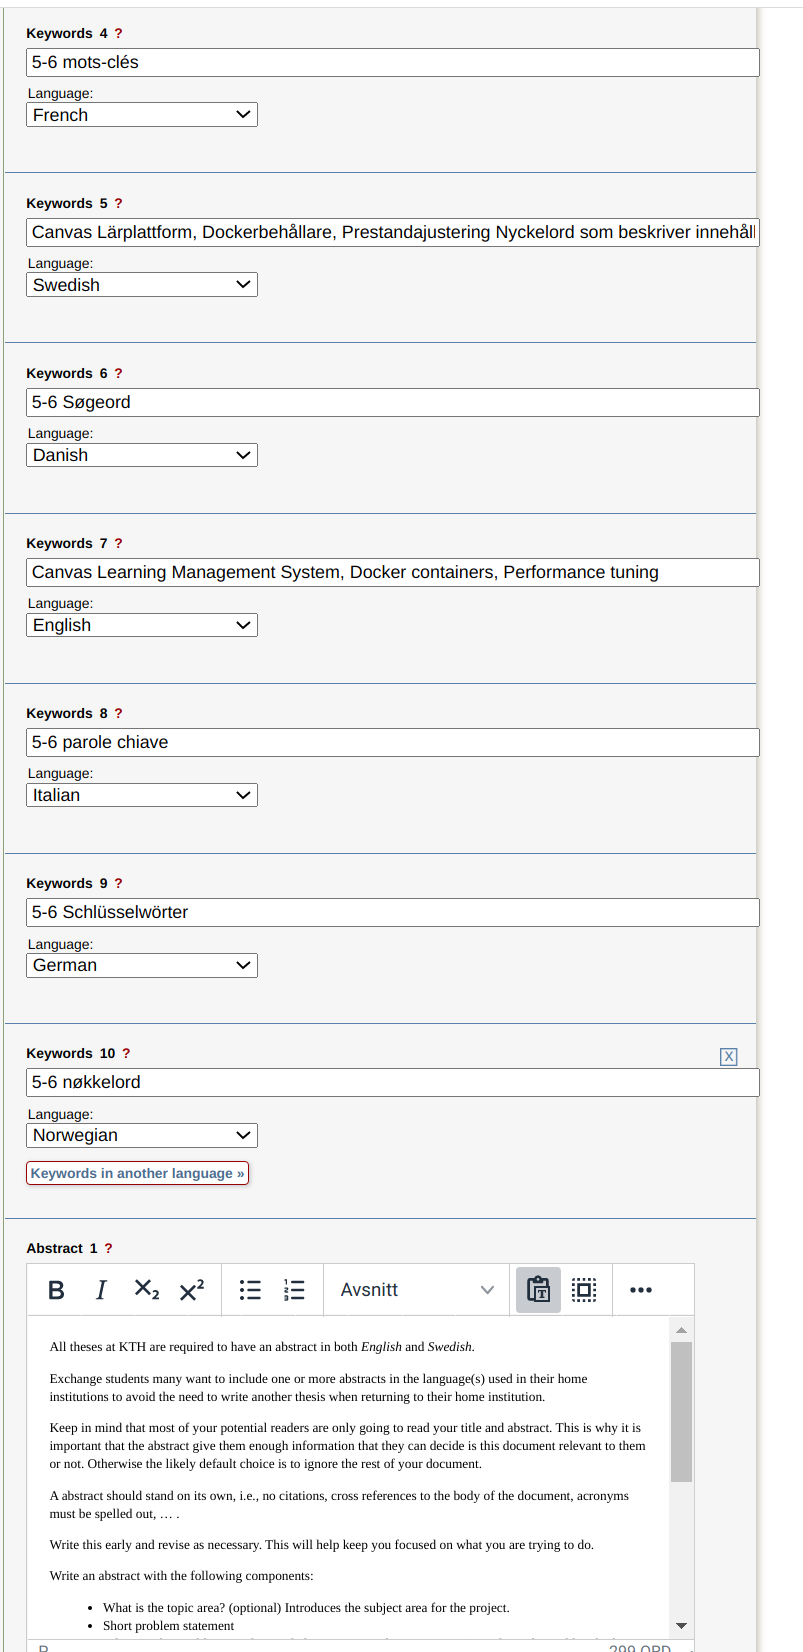
\includegraphics[width=0.65\textwidth]{README_notes/README-examiner-figures/import-d-Screenshot_20210626_234735.png}}
  \end{center}
  \caption[Imported document (part 4)]{Imported document (part 4) – more keywords are shown as well as the abstract in English}
  \label{fig:divaImport8}
\end{figure}
\FloatBarrier

\begin{figure}[!ht]
  \begin{center}
    \fbox{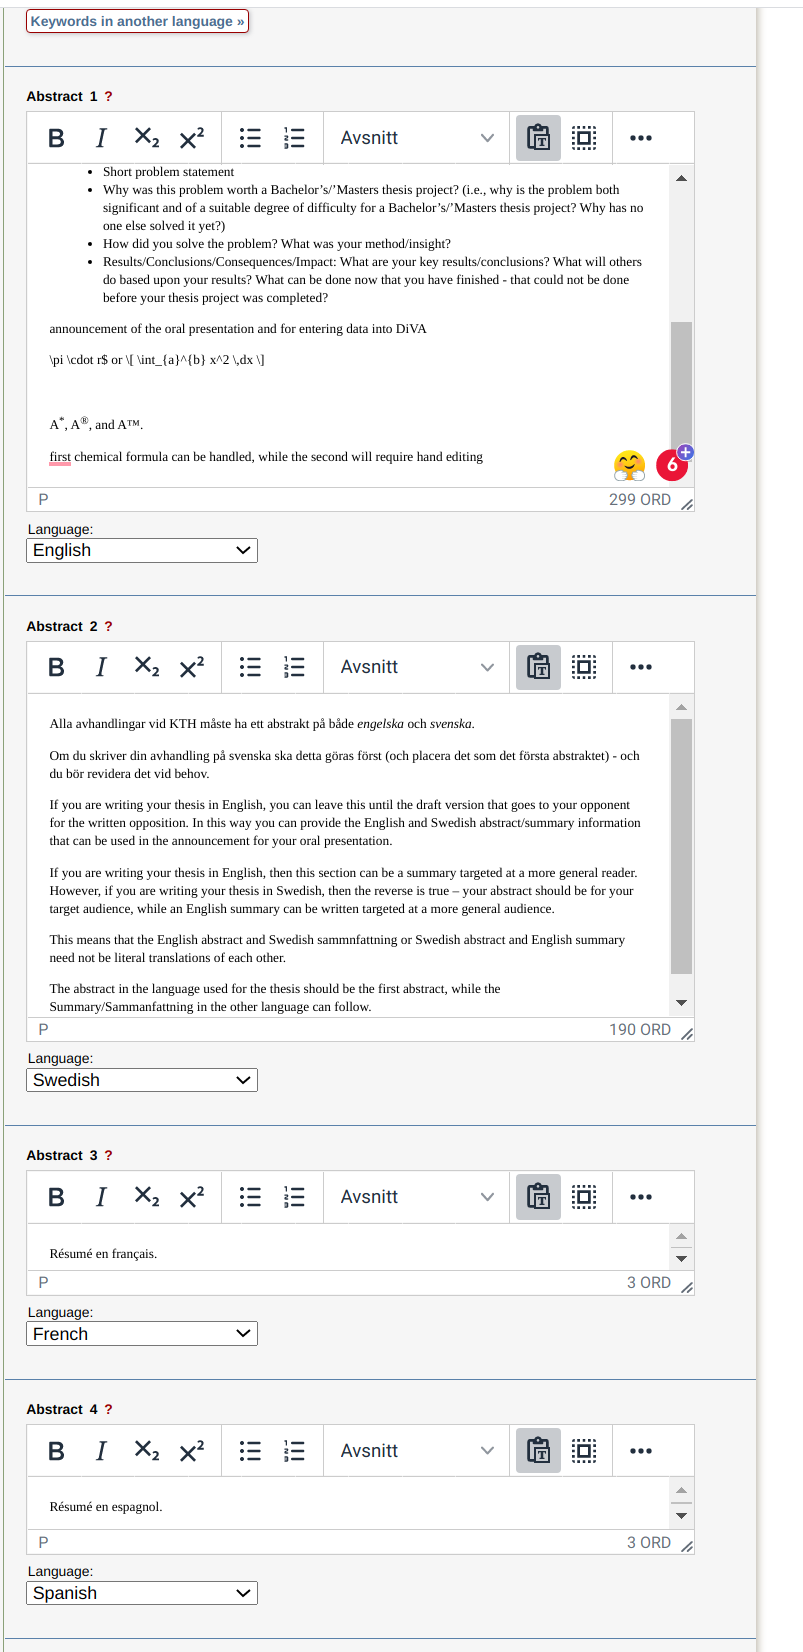
\includegraphics[width=0.65\textwidth]{README_notes/README-examiner-figures/import-e-Screenshot_20210626_235408.png}}
  \end{center}
  \caption{[Imported document (part 5)]Imported document (part 5) – the bottom of the Engish abstract is shown .- showing some of the formatted information that can be shown. Additionally, the Swedish and other abstracts are shown.}
  \label{fig:divaImport9}
\end{figure}
\FloatBarrier

\begin{figure}[!ht]
  \begin{center}
    \fbox{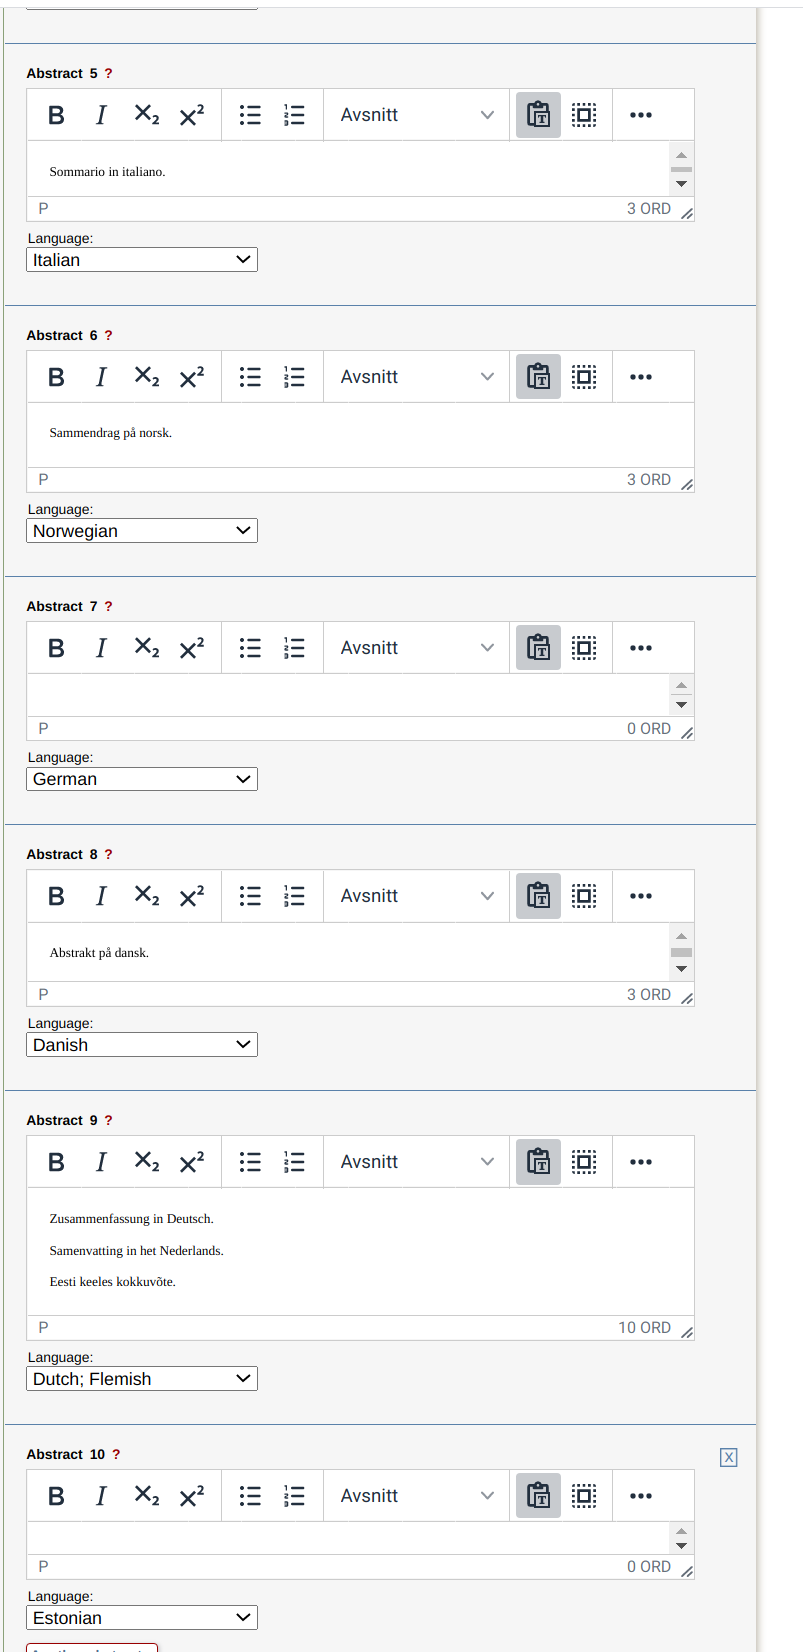
\includegraphics[width=0.7\textwidth]{README_notes/README-examiner-figures/import-f-Screenshot_20210626_235447.png}}
  \end{center}
  \caption[Imported document (part 6)]{Imported document (part 6) – yet more abstracts}
  \label{fig:divaImport10}
\end{figure}
\FloatBarrier
\Cref{fig:divaImport11} shows the three supervisors. The first two have KTH affiliations and the third is from an external organization.
\begin{figure}[!ht]
  \begin{center}
    \fbox{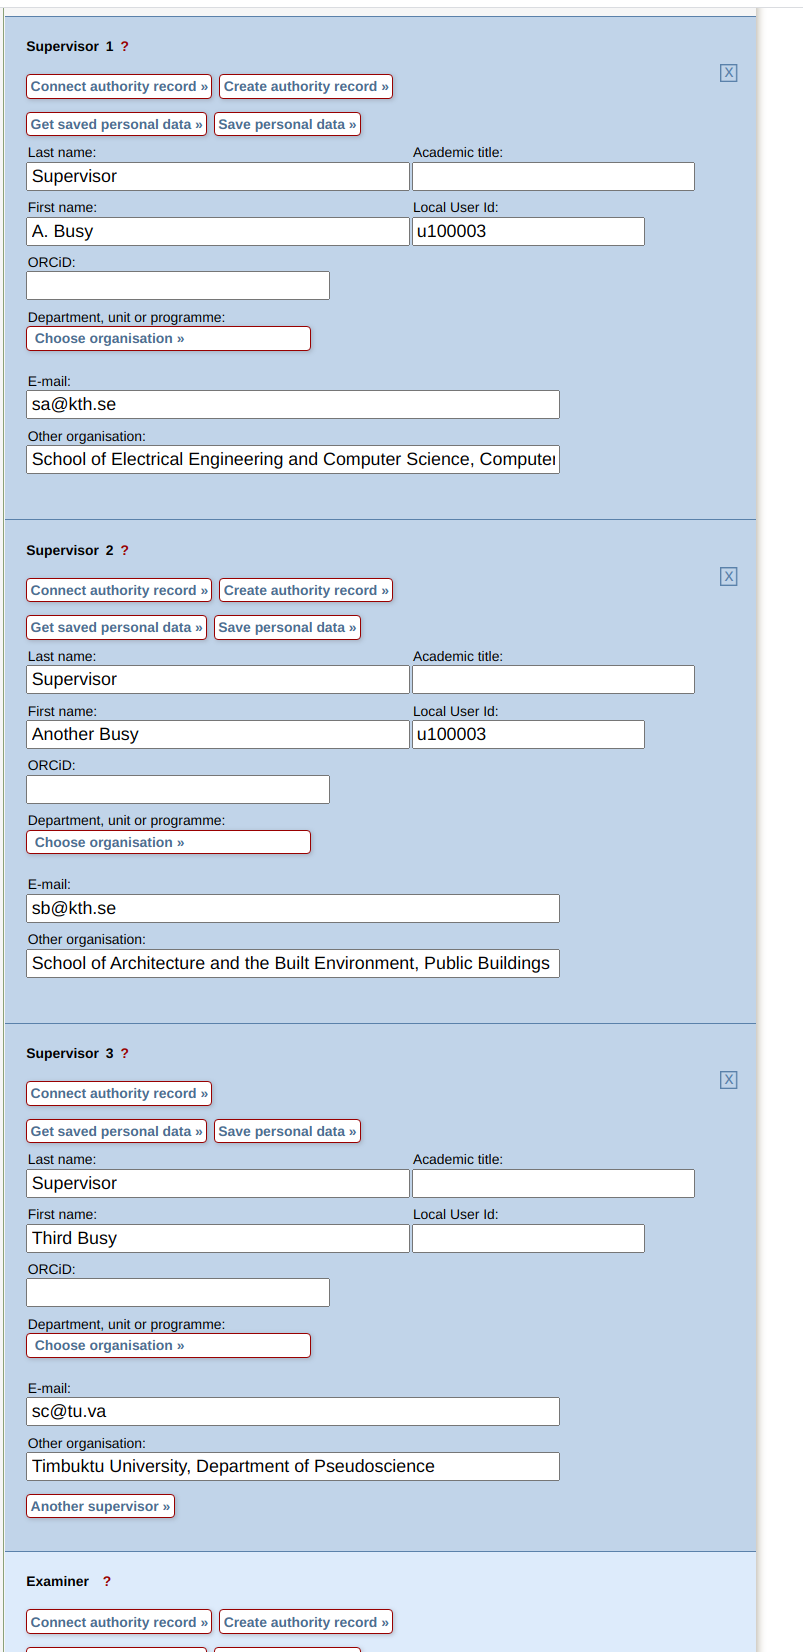
\includegraphics[width=0.7\textwidth]{README_notes/README-examiner-figures/import-g-Screenshot_20210626_235510.png}}
  \end{center}
  \caption[Imported document (part 7)]{Imported document (part 7) – the supervisors are shown}
  \label{fig:divaImport11}
\end{figure}
\newpage

\begin{figure}[!ht]
  \begin{center}
    \fbox{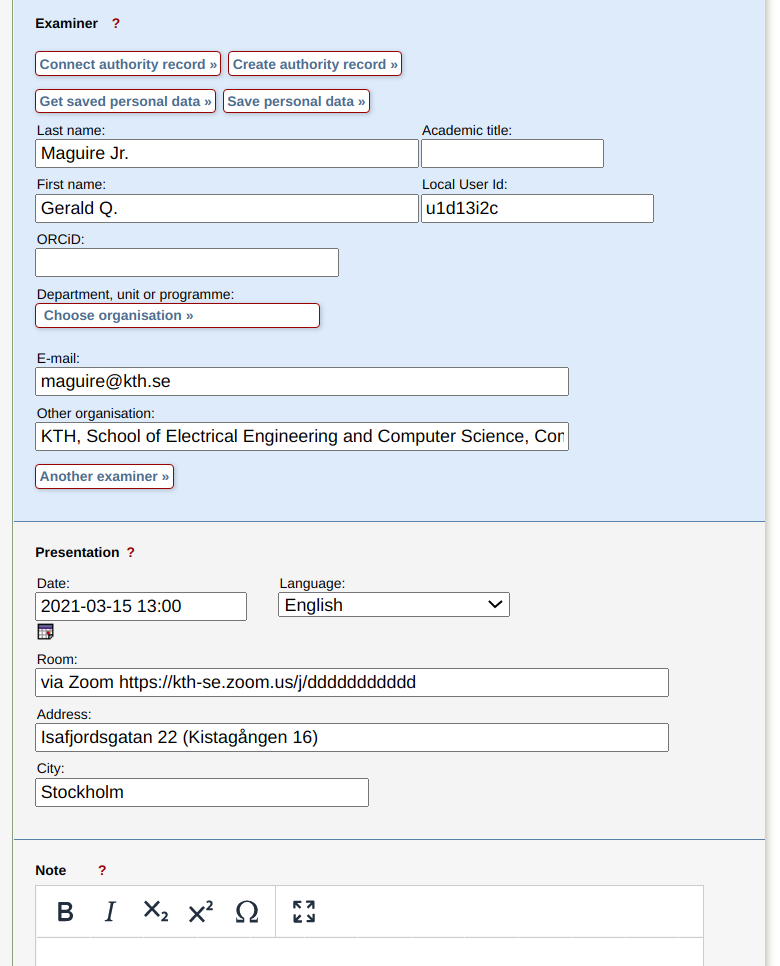
\includegraphics[width=1\textwidth]{README_notes/README-examiner-figures/import-h-Screenshot_20210626_235557.png}}
  \end{center}
  \caption[Imported document (part 8)]{Imported document (part 8) – the examiner is shown along with the information about the oral presentation}
  \label{fig:divaImport12}
\end{figure}
\clearpage


	

\subsection{Limitations}
I was initially unable to get the KTH affiliations correctly entered. I think that it is because I did not understand the description of how to do this at: \url{ https://wiki.epc.ub.uu.se/pages/viewpage.action?pageId=27466001}  where it says:
\babelpolyLangStart{swedish}
För att göra en sådan koppling skall dels ”affiliation” finnas i personelementet dels ett name-element med ID i xlink:href samt ett namePart-element med samma namn som affiliation. Om man har bägge nedanstående element i exemplet kommer Urban Ericsson automatiskt att kopplas till Universitetsbiblioteket i Uppsala vid importen. Om enbart personelementet finns men inte det andra kommer Urban Ericsson att få Uppsala universitet, Universitetsbiblioteket som ”Annat lärosäte” vid importen.
\babelpolyLangStop{swedish}
I did not find any examples of how to do what they describe. The result is that all of my affiliations information ended up in the "Other university" field.

I was also unable to get the issue number to appear, even though it seems to be set - since if you click on the box after the MODS import, it knows the value.  Note that for testing, I forced the TRITA series to be "TRITA-ICT-EX" since this is the actual series that is in the earlier (test) version of DiVA.

Finally, it seems that DiVA does not import the cooperation data at all: according to \url{https://wiki.epc.ub.uu.se/display/divainfo/Externt+samarbete}

The first two limitations have been overcome as described in\linebreak[4] \Cref{sec:limitationsOvercome}.

\subsection{Limitations overcome}
\label{sec:limitationsOvercome}
This section describes how two of the limitations were overcome.

\subsubsection{Entering number in series}
The first limitation to be over come was entering the particular number in the series for a TRITA number. \Cref{fig:numberInSeriesCorrectlyEntered} shows the value being entered. The error was in the structure of the object, the working version is shown in \Cref{lst:seriesNumber}. My earlier error was due to having the \texttt{<identifier type="issue number">2021:00</identifier>} \textit{within} the \texttt{<titleInfo>}.
 
 
\begin{figure}[!ht]
  \begin{center}
    \fbox{
\includegraphics[width=1\textwidth]{README_notes/README-examiner-figures/Number_in_series_correctly_entered.png}}
  \end{center}
  \caption{Number in series correctly entered}
  \label{fig:numberInSeriesCorrectlyEntered}
\end{figure}
\Needspace*{8\baselineskip}
\begin{lstlisting}[language={XML}, caption={MODS data for series}, label=lst:seriesNumber]
<relatedItem  type="series">
	      <titleInfo><title>TRITA-EECS-EX</title>
		<identifier type="local">16855</identifier>
	      </titleInfo>
	      <identifier type="issue number">2021:00</identifier>
</relatedItem >
\end{lstlisting}

\FloatBarrier

\subsubsection{Including KTH affiliations}
Earlier, those with KTH affiliations were appearing in the “Other organization” field. The error in my understanding was how the controlled fields for the KTH authors was being used\footnote{These so-called "controlled" fields have specific values that are permitted and these have numeric IDs assigned by the DiVA Consortium.}. We will start by looking at the two KTH affiliated supervisors (see \Cref{fig:twoKTHsupervisors}), the third supervisor (see \Cref{fig:thirdSupervisor}), and the examiner (see \Cref{fig:examiner}). The MODS data for these four people is shown in \Cref{lst:reducedModesExaminerAndSupervisors} and the “magic” \textbf{corporate name} MODS data is shown in \Cref{lst:reducedModesCorpNames}. The trick is that there needs to be corporate name MODS data for each of the possible affiliations – as this is the way that one passes the DiVA numeric code via the \texttt{xlink} information. Note that in the case of the examiner, two different affiliations were specified and there was a corporate name entry for each of them. Moreover, the key is just to have test extra corporate name entries, only one needs to be for the publishers, as shown in \Cref{lst:reducedModesCorpNames} – with the results in \Cref{fig:twoSupervisorsReducedMODS} and shown \Cref{fig:examinerReducedMODS}.

\textbf{NB}: The ICT affiliations (and DiVA codes) were used and the pictures are all from the test DiVA environment: \url{https://kth.test.diva-portal.org/dream/import/importList.jsf}.

\begin{figure}[!ht]
  \begin{center}
    \fbox{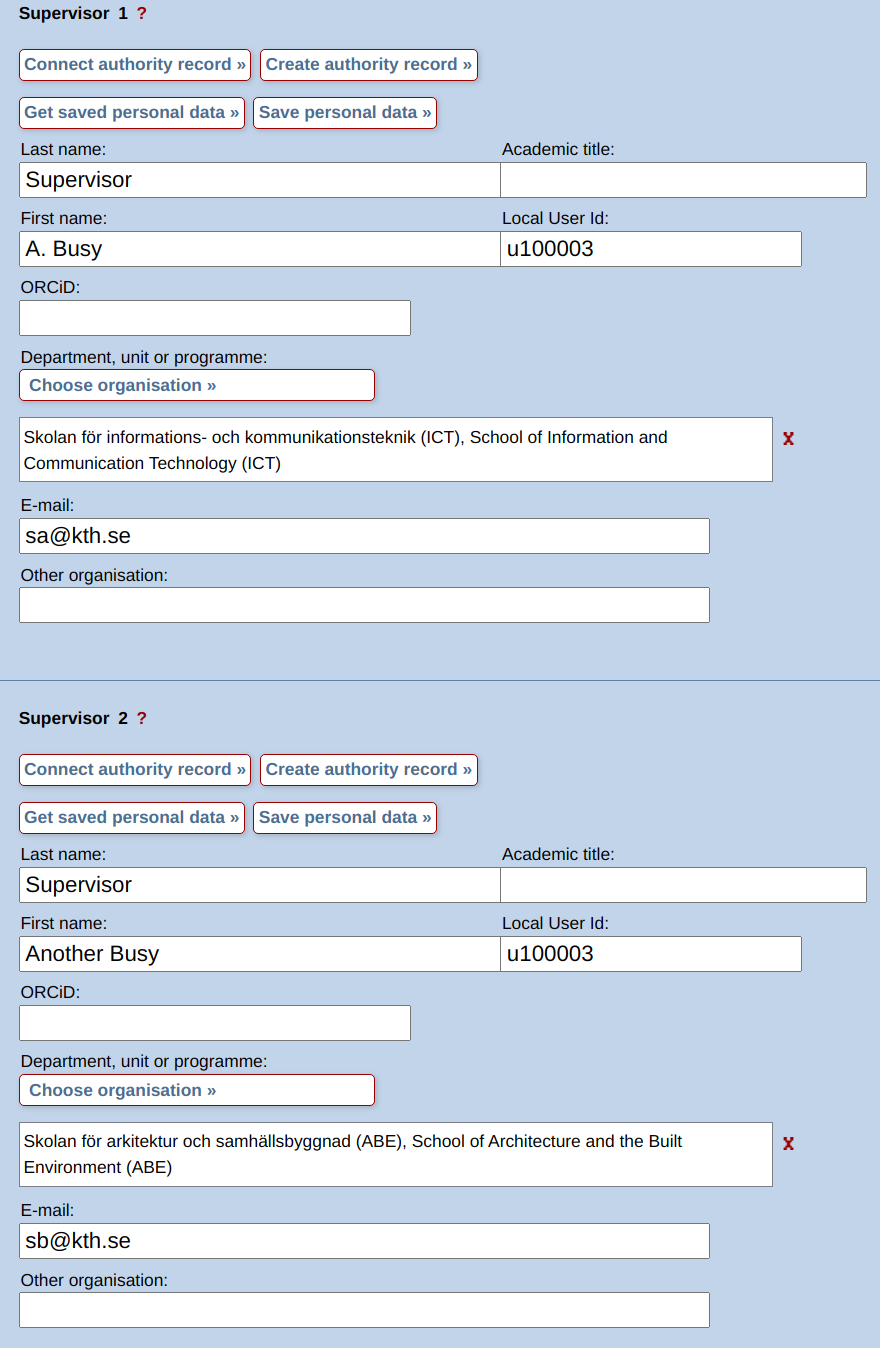
\includegraphics[width=0.9\textwidth]{README_notes/README-examiner-figures/two_KTH_supervisors_in_different_schools.png}}
  \end{center}
  \caption{Two KTH supervisors in different schools}
  \label{fig:twoKTHsupervisors}
\end{figure}
\FloatBarrier
\begin{figure}[!ht]
  \begin{center}
    \fbox{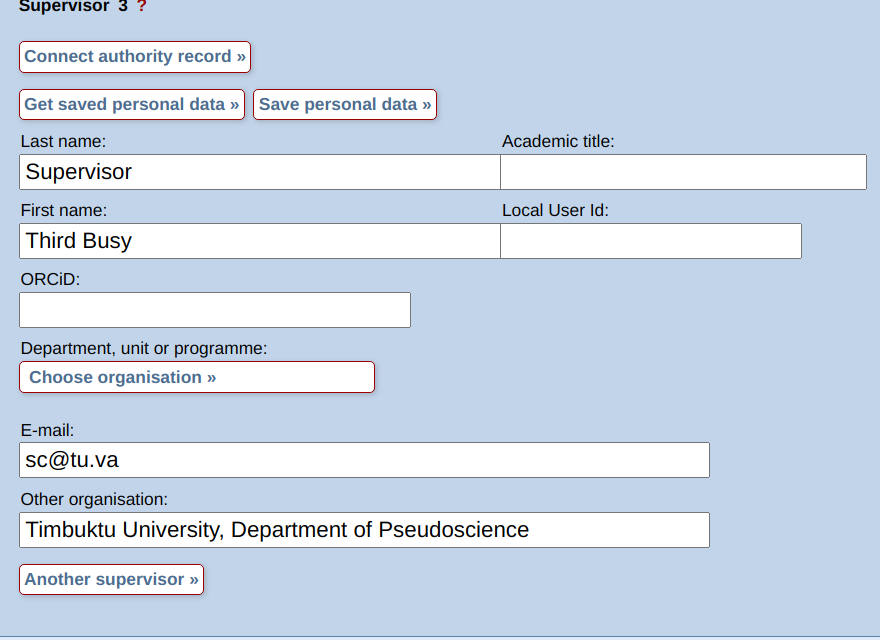
\includegraphics[width=1\textwidth]{README_notes/README-examiner-figures/third_supervisor.png}}
  \end{center}
  \caption{Third supervisor}
  \label{fig:thirdSupervisor}
\end{figure}
\FloatBarrier
\begin{figure}[!ht]
  \begin{center}
    \fbox{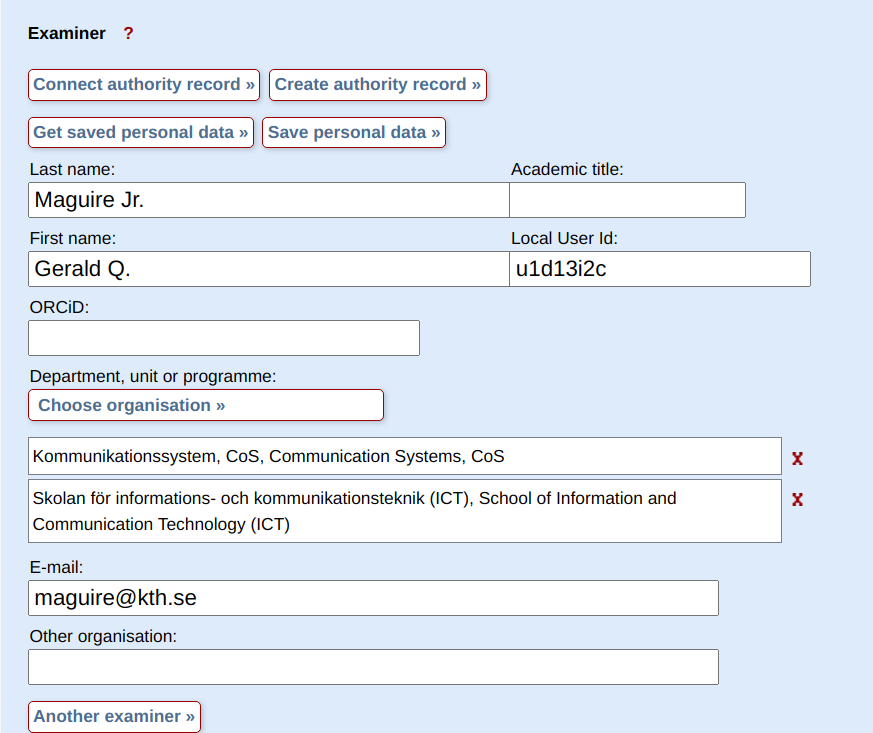
\includegraphics[width=1\textwidth]{README_notes/README-examiner-figures/examiner_affiliation.png}}
  \end{center}
  \caption{Examiner}
  \label{fig:examiner}
\end{figure}
\clearpage

\begin{lstlisting}[language={XML}, caption={MODS data for the supervisors and examiners}, label=lst:reducedModesExaminerAndSupervisors]
<name type="personal" authority="kth" xlink:href="u1d13i2c">
      <namePart type="family">Maguire Jr.</namePart>
      <namePart type="given">Gerald Q.</namePart>
      <description>email=maguire@kth.se</description>
      <affiliation>KTH, Skolan för informations- och kommunikationsteknik (ICT), Kommunikationssystem, CoS</affiliation>
      <affiliation>KTH, Skolan för informations- och kommunikationsteknik (ICT)</affiliation>
      <role><roleTerm type="code" authority="marcrelator">mon</roleTerm></role>
</name>

<name type="personal" authority="kth" xlink:href="u100003">
      <namePart type="family">Supervisor</namePart>
      <namePart type="given">A. Busy</namePart>
      <affiliation>KTH, Skolan för informations- och kommunikationsteknik (ICT)</affiliation>
      <description>email=sa@kth.se</description>
      <role><roleTerm type="code" authority="marcrelator">ths</roleTerm></role>
</name>

<name type="personal" authority="kth" xlink:href="u100003">
      <namePart type="family">Supervisor</namePart>
      <namePart type="given">Another Busy</namePart>
      <affiliation>KTH, Skolan för arkitektur och samhällsbyggnad (ABE)</affiliation>
      <description>email=sb@kth.se</description>
      <role><roleTerm type="code" authority="marcrelator">ths</roleTerm></role>
</name>

<name type="personal">
      <namePart type="family">Supervisor</namePart>
      <namePart type="given">Third Busy</namePart>
      <affiliation>Timbuktu University, Department of Pseudoscience</affiliation>
      <description>email=sc@tu.va</description>
      <role><roleTerm type="code" authority="marcrelator">ths</roleTerm></role>
</name>
\end{lstlisting}
\clearpage

\begin{lstlisting}[language={XML}, caption={Corporate name data in MODS data for the affiliations}, label=lst:reducedModesCorpNames]
<name type="corporate" authority="kth" xlink:href="5994">
      <namePart>KTH</namePart>
      <namePart>Skolan för informations- och kommunikationsteknik (ICT)</namePart>
      <role><roleTerm type="code" authority="marcrelator">pbl</roleTerm></role>
</name>

<name type="corporate" authority="kth" xlink:href="5998">
      <namePart>KTH</namePart>
      <namePart>Skolan för informations- och kommunikationsteknik (ICT)</namePart>
      <namePart>Kommunikationssystem, CoS</namePart>
      <role><roleTerm type="code" authority="marcrelator">pbl</roleTerm></role>
</name>

<name type="corporate" authority="kth" xlink:href="5850">
      <namePart>KTH</namePart>
      <namePart>Skolan för arkitektur och samhällsbyggnad (ABE)</namePart>
      <role><roleTerm type="code" authority="marcrelator">pbl</roleTerm></role>
</name>
\end{lstlisting}

\begin{lstlisting}[language={XML}, caption={Reduced MODS for corporate names more}, label=lst:reducedModesCorpNamesMore]
<name type="corporate" authority="kth" xlink:href="5994">
      <namePart>KTH</namePart>
      <namePart>Skolan för informations- och kommunikationsteknik (ICT)</namePart>
      <role><roleTerm type="code" authority="marcrelator">pbl</roleTerm></role>
</name>
<name type="corporate" authority="kth" xlink:href="5998">
      <namePart>KTH</namePart>
      <namePart>Skolan för informations- och kommunikationsteknik (ICT)</namePart>
      <namePart>Kommunikationssystem, CoS</namePart>
</name>
<name type="corporate" authority="kth" xlink:href="5850">
      <namePart>KTH</namePart>
      <namePart>Skolan för arkitektur och samhällsbyggnad (ABE)</namePart>
</name>
\end{lstlisting}
\clearpage

\begin{figure}[!ht]
  \begin{center}
    \fbox{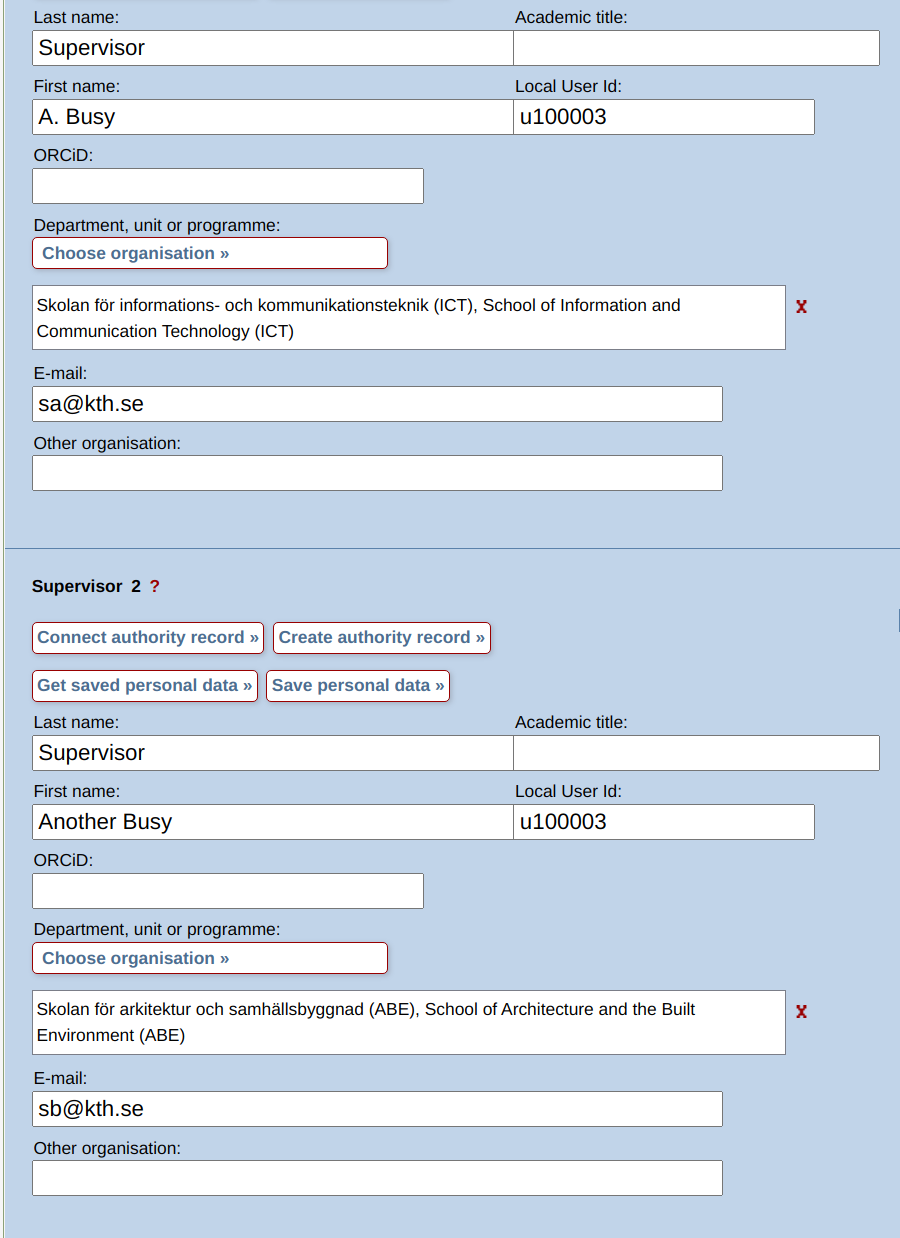
\includegraphics[width=1\textwidth]{README_notes/README-examiner-figures/two_supervisors_reduced_mods.png}}
  \end{center}
  \caption{The two supervisors with the reduced MODS for corporate names}
  \label{fig:twoSupervisorsReducedMODS}
\end{figure}

\begin{figure}[!ht]
  \begin{center}
    \fbox{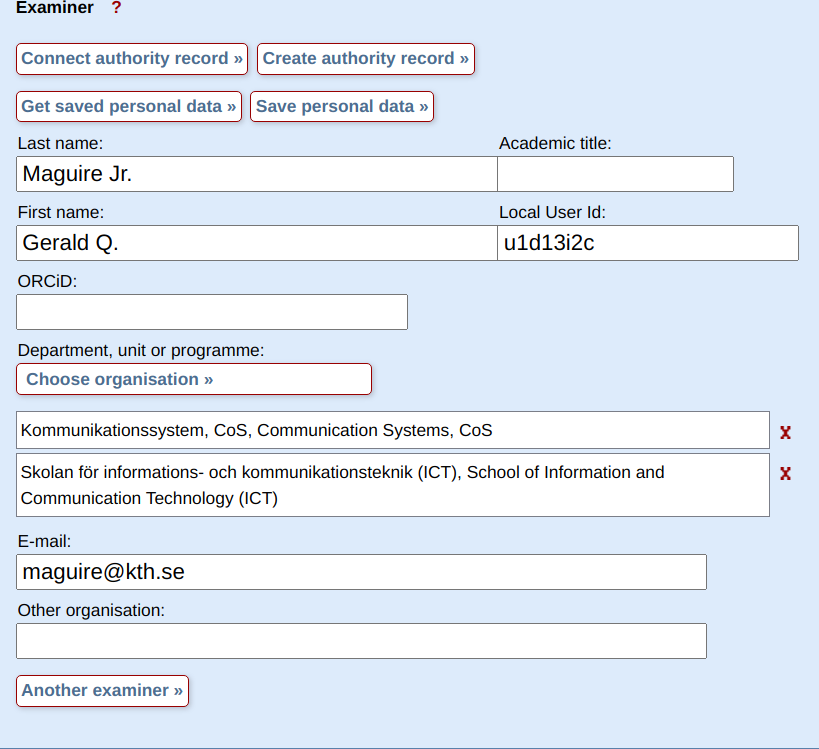
\includegraphics[width=1\textwidth]{README_notes/README-examiner-figures/examiner_with_reduced_mods.png}}
  \end{center}
  \caption{The examiner with the reduced MODS for corporate names}
  \label{fig:examinerReducedMODS}
\end{figure}
\clearpage

\section{Some enhancements}
\label{sec:someEhnahncements}
The enhancements described in \Cref{sec:enhancementsToTemplate} are enhancements to the template and supporting programs to avoid the user having to enter some information on the command line when making a cover and to make the information better available for a future DiVA entry. The enhancements described in \Cref{sec:betterSupportForMathInAbstracts} are to better support mathematical expressions in abstracts. \Cref{sec:AcronymsInAbstracts} describes support for acronyms in abstracts. \Cref{sec:URLSinAbstracts} describes the state of support for URLs in abstracts. \Cref{sec:gettingPDFfromCanvasAssignment} describes a program that can extract an assignment from a Canvas course room and optionally feed it to the program to extract the pseudo-JSON information.

\subsection{Enhancements to template and supporting programs}
\label{sec:enhancementsToTemplate}
Add better support for the subject area (or areas in the case of a student doing both a Civ. Ing. Degree and a Master’s degree).

\subsection{Better support for mathematical expressions in abstracts}
\label{sec:betterSupportForMathInAbstracts}
\LaTeX~in the abstracts is passed through to the pseudo JSON in the “For DIVA” text at the end of the thesis. When preparing this text for Cortina calendar entries or for the announcement in the Canvas course room (and for the calendar event in the course room) some simple \LaTeX~commands are converted to HTML. As few abstracts (in the many abstracts that I looked at in DiVA) have equations I have only done these few transformations. However, if there were to be more use of equations, then there is probably a need to support them for the different platforms (Cortina (see Appendix~\ref{sec:BetterSupportforMathinCortina}), DiVA (see Appendix~\ref{sec:SupportForMathematicsInDiVA}), and Canvas (see Appendix~\ref{sec:betterSupportMathInCortinaAndCourseCalendar})).


\subsubsection{Better support for mathematics in Canvas course announcement and course calendar}
\label{sec:betterSupportMathInCortinaAndCourseCalendar}
As of 2021-06-18, MathJAX and URLs are now supported in the Canvas course room announcement and calendar.
Using the Overleaf project: \url{https://www.overleaf.com/read/qsyddnhhvkgr} to provide a test source document. The results can be seen in \Cref{fig:equationsInAnnouncement}. These results and the results shown in Appendix~\ref{sec:BetterSupportforMathinCortina} were generated using the commands in \Cref{lst:jsonToCalendar3}.
\begin{figure}[!ht]
  \begin{center}
    \fbox{
\includegraphics[width=1\textwidth]{README_notes/README-examiner-figures/announcement_with_equation.png}}
  \end{center}
  \caption{Examples of equations in an announcement}
  \label{fig:equationsInAnnouncement}
\end{figure}
\FloatBarrier
\Needspace*{8\baselineskip}
\begin{lstlisting}[language={bash}, caption={Commands to produce the JSON and make the calendar entries and announcement}, label=lst:jsonToCalendar3]
./extract_pseudo_JSON-from_PDF.py --pdf abstracts_with_equations_in_them.pdf --json eqtest.json
./JSON_to_calendar.py -c 11 --config config-test.json --json eqtest.json
\end{lstlisting}

\FloatBarrier

Note that block/display math are displayed in the Canvas summary for the announcements and cause Canvas to stop summarizing the abstract. The cause for this is not yet known, but has been reported to e-learning ([\#ID:KTH-INC-3677258\#]) and I have blogged about it in the Canvas Community. An example of the equation being displayed in the summary of the announcement is shown in \Cref{fig:announcementSummary}. The announcement is shown in \Cref{fig:announcementWithEquation} while \Cref{lst:HTMLannouncement} shows the HTML for this announcement.

\begin{figure}[!ht]
  \begin{center}
    \fbox{
\includegraphics[width=1\textwidth]{README_notes/README-examiner-figures/Announcement_summary.png}}
  \end{center}
  \caption{Announcement summary}
  \label{fig:announcementSummary}
\end{figure}
\FloatBarrier

\begin{figure}[!ht]
  \begin{center}
    \fbox{
\includegraphics[width=1\textwidth]{README_notes/README-examiner-figures/announcement_with_equation.png}}
  \end{center}
  \caption{Announcement with equation}
  \label{fig:announcementWithEquation}
\end{figure}
\FloatBarrier
\Needspace*{18\baselineskip}
\begin{lstlisting}[language={HTML}, caption={HTML for the announcement}, label=lst:HTMLannouncement]
<h2 lang="en">Abstract</h2>
<p>All theses at KTH are required to have an abstract in both <i>English</i> and <i>Swedish</i>.</p>
<p>Exchange students many want to include one or more abstracts in the language(s) used in their home institutions to avoid the need to write another thesis when returning to their home institution.</p>
<p><span class="math-tex">\(\pi \cdot r\)</span> or <span class="math-tex">\[ \int_{a}^{b} x^2 \,dx \]</span></p>
<p>Some more text: A<sup>*</sup>, A<sup>&reg;</sup>, and A&trade;.</p>
<p><strong>Keywords:</strong> <em>Canvas Learning Management System, Docker containers, Performance tuning </em></p>
\end{lstlisting}


Via XXXXX at IT-support, I raised the question about why the block equations were appearing in the summary of the announcement.

The response from Instructure support regarding the block equations showing up in the summary of the announcements was\footnote{Note that the URLs have been added in parenthesis.}:
\begin{quote}
Thank you for reaching back out.  I did some testing on this and I have a few things to point out and some follow up questions.

First off, the syntax of the block equation isn't the officially supported format.  The inline equation is correct with the \textbackslash(...\textbackslash) delimiters, but the block equation should be formatted with dollar signs, as \$\$...\$\$.  I see the square bracket delimiters \textbackslash[...\textbackslash] are working currently, but this is not the officially supported format and may not always work.  Information on this can be found in these release notes (\url{https://community.canvaslms.com/t5/Canvas-Releases/Canvas-Release-Notes-2021-02-20/ta-p/434781\#toc-hId-698876024}).

Regardless of that though, I wanted to get clarification on the issue at hand.  When I open the announcement, I see both the inline and block equations, but I see only the block equation when viewing it on the main Announcements page.  Is this specifically what you're reporting?  (sandbox screenshot for reference (\url{https://share.getcloudapp.com/jkuPOKRD})  If so, this is because the Announcements page only shows a snippet of the text, so an inline equation beyond the point the text is truncated isn't treated any differently than the rest of the text not shown.  It is interesting that Canvas decides to show the block equation in this view though.  Having that removed from the preview would best be submitted as a feature request (\url{https://community.canvaslms.com/t5/forums/postpage/board-id/ideas/search-before-post-mode/true} ).

If the issues you're reporting are when the full announcement is open, I'm not seeing the same behavior on this end.  If that's the case, can you provide a screenshot of what you're seeing?  And does the behavior persist in a different browser?

Let me know if I've misinterpreted anything or if there are any other questions as well.  We'll be happy to help.  Thanks and have a great day!"
\end{quote}

The response from someone at Instructure shows that Instructure got the same behavior from the block equations in the snippets of the announcements.  A screenshot of this behavior is shown in \Cref{fig:screenSHotOfBlockEquation}. However, their solution for this is to suggest that we submit a feature request. 

\begin{figure}[!ht]
  \begin{center}
    \fbox{
\includegraphics[width=1\textwidth]{README_notes/README-examiner-figures/block_equation_in_Canvas.png}}
  \end{center}
  \caption{The screenshot mentioned above}
  \label{fig:screenSHotOfBlockEquation}
\end{figure}
\FloatBarrier



\subsubsection{Better support for mathematics in Cortina}
\label{sec:BetterSupportforMathinCortina}

YYYYYY indicated that CORTINA supports mathematical expressions using a class name of “math-tex” and gave an example:
%% <span class=\"math-tex\">\\(x = {-b \\pm \\sqrt{b^2-4ac} \\over 2a}\\)</span>
\begin{quote}
$<$span class=\textbackslash"math-tex\textbackslash"$>$\textbackslash\textbackslash(x = {-b \textbackslash\textbackslash pm \textbackslash\textbackslash sqrt\{b\^{}2-4ac\} \textbackslash\textbackslash over 2a}\textbackslash\textbackslash)$<$/span$>$
\end{quote}


\noindent He also noted that Cortina does not allow images in paragraphs, so the solutions for Cortina and DiVA have to be different.

An important note about the above example is that \textbackslash over is deprecated and one should use \textbackslash frac{}{} or one of its variance instead; hence, I used this version of the equation in my source \LaTeX~file.
\clearpage
\Cref{fig:cortinaExample1} shows the entry in the Cortina calendar, while \Cref{fig:cortinaExample2} and \Cref{fig:cortinaExample3} show zoomed in views of the equations.
\begin{figure}[!ht]
  \begin{center}
    \fbox{
\includegraphics[width=0.65\textwidth]{README_notes/README-examiner-figures/Cortina_exaample1.png}}
  \end{center}
  \caption{Equations in Cortina calendar entry}
  \label{fig:cortinaExample1}
\end{figure}
\FloatBarrier

\begin{figure}[!ht]
  \begin{center}
    \fbox{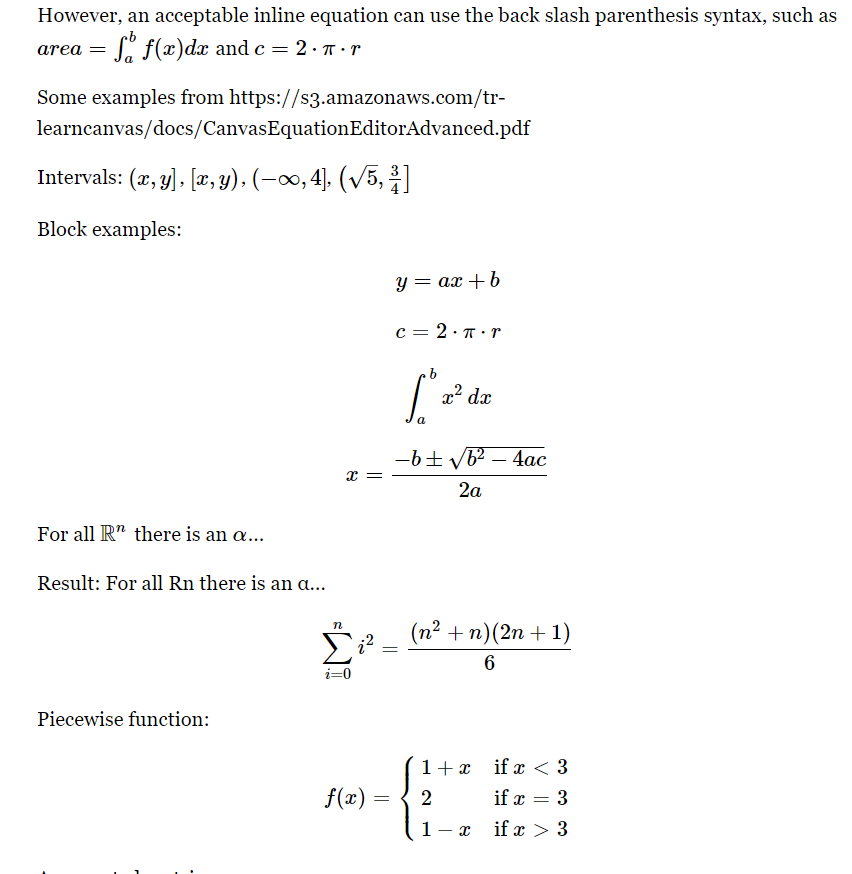
\includegraphics[width=1\textwidth]{README_notes/README-examiner-figures/cortina-eqn-zoom1.png}}
  \end{center}
  \caption{Zoom in on part of the Cortina calendar entry}
  \label{fig:cortinaExample2}
\end{figure}
\FloatBarrier

\begin{figure}[!ht]
  \begin{center}
    \fbox{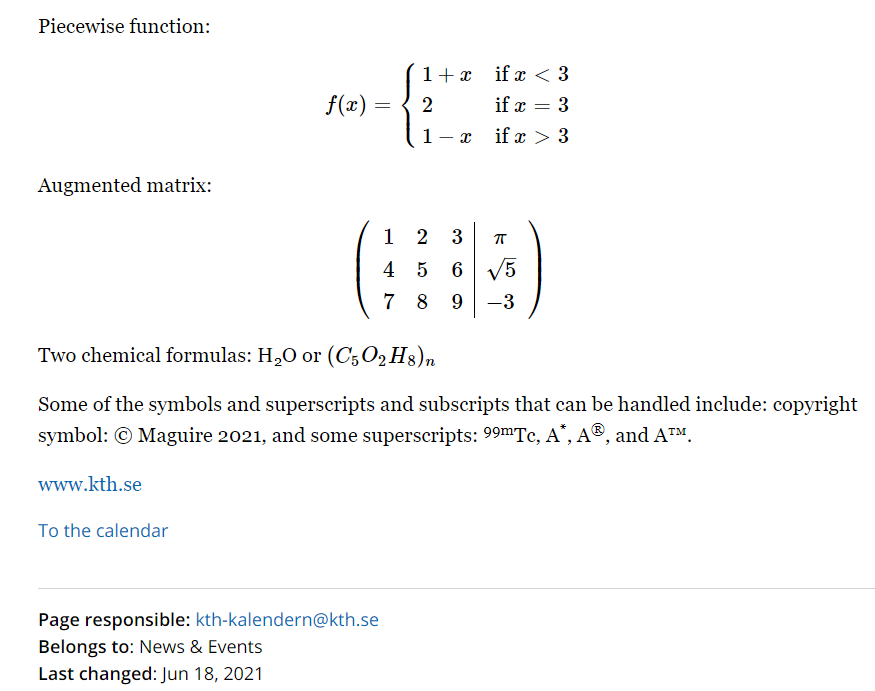
\includegraphics[width=1\textwidth]{README_notes/README-examiner-figures/cortina-eqn-zoom2.png}}
  \end{center}
  \caption{Zoom in on lower part of the Cortina calendar entry}
  \label{fig:cortinaExample3}
\end{figure}
\FloatBarrier
 

\subsubsection{Support for mathematics in DiVA}
\label{sec:SupportForMathematicsInDiVA}
In contrast to Canvas and Cortina, DiVA uses pictures (although these can have a \LaTeX~expression as an “alt” description of the image contents).
The code does not (yet) support the addition of equations to the DiVA entry of the abstracts.
The current DiVA user interface seems to strip out the math-tex classes, \ie 

% <span class='math-tex'>\[ \int_{a}^{b} x^2 \,dx \]</span> 
\begin{quote}
$<$span class=\textbackslash"math-tex\textbackslash"$>$\textbackslash [ \textbackslash int\_\{a\}\^{}\{b\} x\^{}  \textbackslash ,dx \textbackslash ] $<$/span$>$
\end{quote}

becomes simply:
% \[ \int_{a}^{b} x^2 \,dx \]
\begin{quote}
\textbackslash [ \textbackslash int\_\{a\}\^{}\{b\} x\^{}2  \textbackslash ,dx \textbackslash ]
\end{quote}
\noindent However, I do not know what happens when this is later displayed by DiVA, \ie whether it will appear as an equation or not.

Fortunately, one can use the picture support as shown in the example below to generate \textbackslash\ widehat\{Err\} over Err:
\begin{quote}
<img src="http://www.diva-portal.org/cgi-bin/mimetex.cgi?\%5Cwidehat\%7BErr\%7D" data-classname="equation" data-title="" />
\end{quote}

\subsection{Acronyms in abstracts}
\label{sec:AcronymsInAbstracts}

As students may use acronyms in abstracts, there is support for the commands: \textbackslash gls{}, \textbackslash glspl{}, \textbackslash Gls{}, \textbackslash Glspl{}, \textbackslash acrlong{}, \textbackslash acrshort{}, and \textbackslash acrfull{}. There is also an optional argument to the extraction program to specify the name of the file with definitions of acronyms using the \texttt{\textbackslash newacronyms\{label\}\{acronym\}\{phrase\}} form of definitions. This optional argument is shown in \Cref{lst:specifyingAcronymsFile}. Note that expanding acronyms are handled independently for the abstracts, so that they are spell out on first use in each abstract. Note also that there is no support for multiple languages for the phrase that is used, \ie the expansion simply uses the phrase defined in the \textbackslash newacronyms definition.
\Needspace*{4\baselineskip}
\begin{lstlisting}[language={bash}, caption={Specifying acronyms file}, label=lst:specifyingAcronymsFile]
./extract_pseudo_JSON-from_PDF.py --pdf xxxx.pdf --json xxxx.json --acronyms acronyms.tex
\end{lstlisting}


Additionally, the commands (from \texttt{defines.tex}) are supported in abstracts: \textbackslash ie, \textbackslash eg, \textbackslash etc, \textbackslash etal, \textbackslash first, \textbackslash second, \textbackslash third, \ldots . Now that all the acronyms are spelled out, there is no problem with them when making a calendar entry or MODS file.

\subsection{URLs in abstracts}
\label{sec:URLSinAbstracts}
Currently URLs in abstracts are supported in Canvas course room announcements and the Canvas calendar, but not in the Cortina calendar – where the URL is simply shown as text.

\subsection{Getting the PDF from a Canvas assignment and optionally extracting JSON}
\label{sec:gettingPDFfromCanvasAssignment}

To simplify getting a PDF file from an Canvas course assignment submission there is a program \texttt{get\_PDF\_submission.py} to help with this.  The program checks that the submission has been graded and has the grade 'complete' and then gets the PDF file submitted for a specified assignment. The generic form of the command and an example are shown in \Cref{lst:getPDFsumbission}. Note that the student's name is used as a prefix of the name of the output file, while the submitted filename is used as the rest of the file name. With the optional [-e] argument, the program runs the extraction program. Note that this program is my Canvas-tools github: \url{https://github.com/gqmaguirejr/Canvas-tools}. 
\Needspace*{4\baselineskip}
\begin{lstlisting}[language={bash}, caption={get\_PDF\_submission program}, label=lst:getPDFsumbission]
./get_PDF_submission.py -c course_id -a assignment_id -u user_id
\end{lstlisting}

The program could be made more user friendly by being able to specify the name of the assignment and the user’s e-mail address or other information to avoid the need to enter the assignment\_id and user\_id. This remain for future work.

%% GQMJr to revise
\subsection{Support for new cover[Section to be revised]}
Given that the cover for 3\textsuperscript{rd} cycle dissertations changed during this academic year I have been expecting that there will be a new format for the cover for 1\textsuperscript{st} and second-cycle thesis. I received a note about this on 2021-06-23. It seems that it will be based upon a PDF form and will come into use this Fall. So I started to do some experiments about filling in their form. An initial program is fill\_in\_template.py and the command line interface and an example are shown in \Cref{lst:newfillinTemplae}.
\Needspace*{8\baselineskip}
\begin{lstlisting}[language={bash}, caption={New fill\_in\_template.py program}, label=lst:newfillinTemplae]
./fill_in_template.py --pdf template.pdf --json data.json
Output: outputs a pdf file named "output.pdf" (currently a fixed name)
Example:
./fill_in_template.py --pdf "KTH_Omslag_Exjobb_Formulär_Final_dummy_EN-20210623.pdf" –json xxxx.json --trita "TRITA-XXX-EX-2021:330"
\end{lstlisting}

Note that the new template is not yet ready for prime time and this program is a simple hack to see if I can mechanically generate the new format of cover. I had to manually adjust the position of the boxes for the title, subtitle, and author (via the code) to fit the actual title of a recent thesis. Ideally the positioning of this text should be done via:
\begin{enumerate}
\item Directly use \LaTeX~or similar program to position the title, subtitle, and author on a page (with the template either as background or as input)

\item Do the computations within the program to compute the size of each box, based on filling the text into a box and computing the sum of the width of the characters and spacing and the heights of the lines to dynamically compute the size of the box. This should also incorporate computation of a fixed leading between the boxes.
\end{enumerate}

Note that the new cover template uses the following fonts: "TheSans B4 SemiLight" and "TheSans B6 SemiBold". I have addressed the problem of making these fonts available from within \LaTeX~(for the 1\textsuperscript{st} alternative) and made a small demonstration of this . Unfortunately, I do not yet understand the font metrics enough to write the code for the 2\textsuperscript{nd} alternative nor do I think it is worth doing this since this is just what a text formatting system does.

Once both the new cover template and the program are more mature the code should get integrated into JSON\_to\_cover.py - with a new option to specify whether you want to "new" or "old" cover.

\section{Accessibility}
\label{sec:accessibility}
Accessibility has been divided into accessibility of the calendar entries (see \Cref{sec:accessibilityOfCalendarEntries}), the cover and PDF files (see \Cref{sec:ccessibilityOfCoverandPDF}), and the template itself (see \Cref{sec:ccessibilityOfTemplateItself}). There is also a subsection regarding improving accessibility (see \Cref{sec:improvingAccessibility}).

\subsection{Calendar entries}
\label{sec:accessibilityOfCalendarEntries}
Note that the calendar entries that are generated in the Canvas course room are as accessible as all content in Canvas (as Instructure tries to follow the W3C Web Content Accessibility Guidelines (WCAG)). The European standard EN 301 549 V2.1.2 (based upon WACG 2.1) are the accessibility guidelines for web content that are recommended in Sweden by DIGG (Myndigheten för digital förvaltning), based upon the presentation by Tommy Olsson of DIGG to the SUNSET SALSA group on 2021-06-03. Moreover, the contents are HTML language tagged, so that a text to speech program that has access within Canvas (such as ReaderSpaker is capable of doing as an LTI app) could read the content with the correct pronunciation for each of the two languages. Note that KTH’s current screen reader solution does \textbf{not} access the HTML of the page and hence it does not use the language tags, thus the user must manually choose the language for output.

The calendar entries in the KTH Calendar are in the same format as the current calendar entries. The structure of these entries have been developed in consultation with XXXXXX (who works with the KTH Web) and the KTH Calendar API developer XXXXX with the additional help of XXXXXX. Note that the last of these was the original developer of the KTH cover generator.

\subsection{Cover and PDF file}
\label{sec:ccessibilityOfCoverandPDF}
The PDF metadata (author(s), title(s), keywords, \etc) is accessible to any programs that uses the PDF metadata (this is a standard feature of PDF files). Unfortunately, there are no provisions for language markup for this data.

No investigations has been made of the accessibility of the KTH cover nor of the contents of the PDF file (\ie the thesis itself). The PDF output by Overleaf appears to be PDF version 1.5 (\ie accessible via Acrobat version 6 or later).

The template makes use of color with with regard to the \texttt{hyperref} colors and \texttt{todonotes}. The \texttt{hyperref} colors are defined as shown in \Cref{lst:colors}.
\Needspace*{12\baselineskip}
\begin{lstlisting}[language={[LaTeX]TeX}, caption={\textbackslash hypersetup}, label=lst:setupHyperRef]
\hypersetup{
	colorlinks  = true,
	breaklinks  = true,
	linkcolor   = \linkscolor,
	urlcolor    = \urlscolor,
	citecolor   = \refscolor,
	anchorcolor = black
}
\end{lstlisting}
Where the colors are defined as (note that the ForestGreen lacks sufficient contrast for readability - so another color should be used to replace it) as shown in ±Cref{lst:colors}.
\Needspace*{6\baselineskip}
\begin{lstlisting}[language={[LaTeX]TeX}, caption={Some colors for hyper references }, label=lst:colors]
\definecolor{ForestGreen} {RGB}{34,  139,  34}
\definecolor{HeraldRed2}   {rgb}{0.81, 0.12, 0.15}

\newcommand{\refscolor} {blue}
\newcommand{\linkscolor}{HeraldRed2}
\newcommand{\urlscolor} {ForestGreen}
\end{lstlisting}

Note that the colors do not encode any special meaning (\ie they could all be turned to black), since the citations are recognizable by their format, the URL (and URI) by linking to an external document, and the links (by linking within the document.

Some additional colors are defined and used for \texttt{todonotes} – they should of of course be removed before the thesis is finalized (as of course all of these issues should have been resolved!). The default background color for todonotes is orange (which is predefined as \#FF7F00 \textbackslash definecolor{orange(colorwheel)}{rgb}{1.0, 0.5, 0.0}). The color for notes in Swedish is aqua (defined as:\textbackslash definecolor{aqua}{rgb}{0.0, 1.0, 1.0}). For notes by the authors to themselves using \textbackslash todoinline are red (defined as \textbackslash definecolor{red}{rgb}{0.7,0.0,0.0}). 

\subsection{Template itself}
\label{sec:ccessibilityOfTemplateItself}
The template itself is written in \LaTeX~using UTF-8 characters. The template uses packages from TeX Live version 2022. It can be compiled with \XeLaTeX\ and \LuaLaTeX\  (note that both natively support UTF-8 input). With \textsc{pdfLaTeX} it needs an initial declaration that it should use UTF-8 input encoding.

The template is designed with a set of options to generate a thesis in English or Swedish\footnote{The option names for both languages are in all lower case letters.} and to use either \textsc{Bib}\TeX~ or \textsc{Bib}\LaTeX, as explained at the top of the main file (see \Cref{lst:document}).
\Needspace*{8\baselineskip}
\begin{lstlisting}[language={[LaTeX]TeX}, caption={\textbackslash documentclass}, label=lst:document]
%% set the default language to english or swedish by passing an option to the documentclass - this handles the inside tile page
% to use bibtex or biblatex - edited the following line:
\documentclass[english, bibtex]{kththesis}
%\documentclass[swedish, biblatex]{kththesis}
\end{lstlisting}

The template is available from Overleaf (both as a template and via a share URL). The template is also available from a github repository at KTH; however, this is not updated as frequently as the Overleaf version of the template.

The text in the template itself (\ie the \texttt{examplethesis.tex} file) is in Swedish and English. The notes regarding the \LaTeX~class file, the various lib files, and the two README files are currently only in English.

The default bibliographic style when using \textsc{Bib}\TeX~is my own adaptation of the IEEE Transactions format (\ie numbered citations, numbered references, references in order of use) with the extension of adding DOIs, URLs, and ISBNs (when relevant).

\subsection{Improving accessibility}
\label{sec:improvingAccessibility}
One method for improving accessibility would be to include the accessibility package, \ie \textbackslash usepackage\{axessibility\} as this would include a comment in the PDF file for each equation with the \LaTeX that generated the equation. However, this package is no longer maintained and is incompatible with many other packages. For an introduction to what the \LaTeX\;project has been working on see “LATEX Tagged PDF|A blueprint for a large Project”\footnote{References
Frank Mittelbach and Chris Rowley, ‘LATEX Tagged PDF|A blueprint for a large project’, TUGboat, vol. 41, no. 3, pp. 292–298, 2020 [Online]. Available: \url{https://www.latex-project.org/publications/2020-FMi-TUB-tb129mitt-tagpdf.pdf}}. Based upon this article and the status of the \texttt{tagpdf} package, I conclude that it is too early to worry about properly tagging PDF files, doing so will have to await the release of a packaged designed for production use.

\section{The structure of the template and the report}
The report in itself (\ie the thesis) has a classical IMRAD structure. In some subject areas, such as mathematics there is a tradition for another structure.
The files and folders in Overleaf (or from GitHub) have the form shown in \Cref{fig:overleafFoldersAndFiles}. Some students add folders per chapter and reduce the main document to a skeleton that includes the other parts of the document.
\begin{figure}[!ht]
  \begin{center}
    \fbox{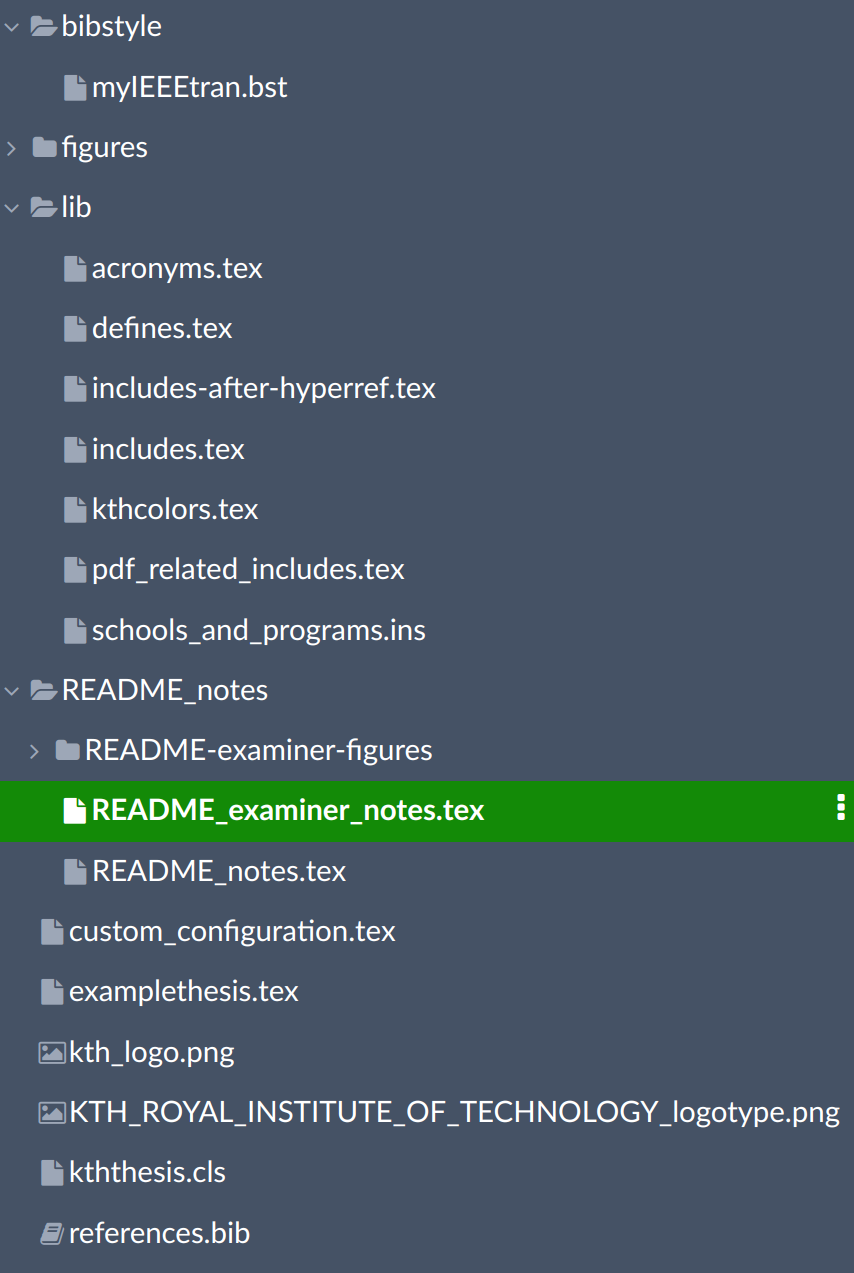
\includegraphics[width=0.5\textwidth]{README_notes/README-examiner-figures/Overleaf_folders_and_files_Screenshot_20220330_150822.png}}
  \end{center}
  \caption{Files and folders in Overleaf template}
  \label{fig:overleafFoldersAndFiles}
\end{figure}
\FloatBarrier

There are currently instructions concerning the template in 
\iflabelexists{ch:READMEnotes}{\Cref{ch:READMEnotes}.}
{xxxx- You have to include the \texttt{README\_notes/README\_notes.tex} file when compiling to get additional information.}
Ideally, these instructions should be available in both English and Swedish; however, a Swedish version remains as future work.

Most students will only need to add acronyms to the \texttt{acronyms.tex} file and perhaps additional packages to \texttt{includes.text} (in some cases these may need to be added to the \texttt{includes-after-hyperref.tex} file if there is a conflict with \texttt{hyperref}).

The \texttt{schools\_and\_programs.ins} and \texttt{old\_schools\_and\_programs.ins} were generated from the data in KOPPS. Students will not have to change these files.
%The \texttt{old\_schools\_and\_programs.ins} file has now been removed from the template.
\clearpage


\section{Generating LaTeX commands for in the student’s thesis source file}
The thesis makes use of a set of \LaTeX~commands to collect information about the student, the supervisor(s), and the examiner. However, how can a student know what their KTHID and other necessary information is?

There are two alternatives:
\begin{itemize}
    \item The examiner or someone can use the method described in \Cref{sec:makeItSimpleFromTheStart} or

    \item They can make use of the program: \texttt{whoami\_for\_latex.py}\footnote{Note that this program requires access to LADOK; hence, it is \textbf{no longer available}. However, a version that does not need LADOK access could be used by a student to get their own information from Canvas, \textit{excluding their program information}; as Canvas does not currently have any source for the student's program information.}.
    
    The \texttt{whoami\_for\_latex.py} program makes use of information from the Canvas course room where the student is enrolled for their degree project. In the examples below we will assume that this is the Canvas course\_id 25434.
\end{itemize}

\Cref{lst:whoami2} shows the case for a student author who has the e-mail address “oscarros@kth.se”. Note that the user is prompted to enter their KTH account name and password (in order to access LADOK). Note that this student has two programs of study listed in LADOK (\ie CDATE and TCSCM). The student will have to manually select one of these and comment out or delete the other. The course code is derived from the section of the course that the user is enrolled in. This section name (in the case of this student: “DA231XVT212”) is reduced to a course code by truncation. The course cycle information is taken from the first digit of the course code. This should work for most course codes, except for one program in architecture which is still using a very old course code.
\Needspace*{28\baselineskip}
\begin{lstlisting}[language={bash}, caption={Generating \LaTeX~commands for a student author}, label=lst:whoami]
./whoami_for_latex.py oscarxxxxxs@kth.se 25434
login_id=oscarxxxxxs@kth.se
\authorsLastname{xxxxxx}
\authorsFirstname{Oscar}
\email{oscarros@kth.se}
\kthid{u1xxxxx}
%\authorsSchool{\schoolAcronym{XXX}}
\programcode{CDATE}
% Note that the following line should be commented out, as the programme is derived from the school_and_Programs.ins information
%\programname{Degree Programme in XXX}
\programcode{TXXXX}
% Note that the following line should be commented out, as the programme is derived from the school_and_Programs.ins information
%\programname{Master's Programme, XXX}
\courseCycle{2}
\courseCode{DA231X}
\end{lstlisting}

\Cref{lst:whoami2} show the case of generating the data for a second author (\textbf{NB} this is only possible for a first-cycle thesis). The actual user data has been anonymized in this figure.
\Needspace*{24\baselineskip}
\begin{lstlisting}[language={bash}, caption={Generating the \LaTeX~data for the second author (in the case of a first-cycle thesis)}, label=lst:whoami2]
./whoami_for_latex.py -2 xxxx@kth.se 22156
\secondAuthorsLastname{xxxxx}
\secondAuthorsFirstname{xxxxx}
\secondemail{xxxx@kth.se}
\secondkthid{u1xxxxx}
\secondAuthorsSchool{\schoolAcronym{XXX}}
%Note that the LaTeX template does not support having students with different programs or course codes
\programcode{CINTE}
% Note that the following line should be commented out, as the programme is derived from the school_and_Programs.ins information
%\programname{Degree Programme in Information and Communication Technology}
\courseCycle{1}
\courseCode{IA150X}
\end{lstlisting}


\Cref{lst:secondAuthor} shows the case where the program has been run to add a second author to a second-cycle thesis, note the warning message in the last line of this figure.

\begin{lstlisting}[language={bash}, caption={Attempting to generate a 2\textsuperscript{nd} author for a second-cycle thesis}, label=lst:secondAuthor]
./whoami_for_latex.py -2 oscarros@kth.se 25434
\secondAuthorsLastname{Rosquis}
\secondAuthorsFirstname{Oscar}
\secondemail{oscarros@kth.se}
\secondkthid{u1tmg8l6}
\secondAuthorsSchool{\schoolAcronym{XXX}}
%Note that the LaTeX template does not support having students with different programs or course codes
\programcode{CDATE}
% Note that the following line should be commented out, as the programme is derived from the \texttt{school_and\_Programs.ins} information
%\programname{Degree Programme in XXX}
\courseCycle{2}
\courseCode{XX200X}
latex_courseCycle=\courseCycle{2}, type=<class 'str'>
%%%% Note that a second-cycle thesis should not have two authors!!!
\programcode{TCSCM}
% Note that the following line should be commented out, as the programme is derived from the \texttt{school_and\_Programs.ins} information
%\programname{Master's Programme, XXX}
\courseCycle{2}
\courseCode{XX200X}
latex_courseCycle=\courseCycle{2}, type=<class 'str'>
%%%% Note that a 2nd cycle thesis should not have two authors!!!
\end{lstlisting}

\Cref{lst:supervisor} shows the case for a supervisor who has the e-mail address “vastberg@kth.se”.  \Cref{lst:examiner} shows the case for an examiner who has the e-mail address “maguire@kth.se”.  Note that the information about the school and department (in the case of a supervisor and examiner) are currently fixed and commented out – so that the user can edit them as necessary.
\Needspace*{10\baselineskip}
\begin{lstlisting}[language={bash}, caption={Generating \LaTeX~commands for a supervisor}, label=lst:supervisor]
./whoami_for_latex.py vastberg@kth.se 25434
%If not the first supervisor, then replace supervisorAs with supervisorBs or supervisorCs as appropriate
\supervisorAsLastname{Västber}
\supervisorAsFirstname{Anders}
\supervisorAsEmail{vastberg@kth.se}
% If the supervisor is from within KTH add their KTHID, School and Department info
%\supervisorAsSchool{\schoolAcronym{XXX}}
%\supervisorAsDepartment{DepartmentName}
\end{lstlisting}
\Needspace*{8\baselineskip}
\begin{lstlisting}[language={bash}, caption={Generating \LaTeX~commands for the examiner}, label=lst:examiner]
./whoami_for_latex.py -e xxx@kth.se 25434
\examinersLastname{ExaminersLastname}
\examinersFirstname{ExaminersFirstname}
\examinersEmail{xxx@kth.se}
% If the examiner is from within KTH add their KTHID, School and Department info
\examinersSchool{\schoolAcronym{XXX}}
\examinersDepartment{DepartmentName}
\end{lstlisting}
 	
The program: whoam\_for\_latex.py is far more powerful that shown in the examples above, it can take other identifiers for the user in instead of an e-mail address, such as a Canvas user\_id or a KTHID. Additionally, rather than specifying the Canvas course room’s course\_id, it is also possible to use the name of the course room and even a nickname (if you have defined a nickname in your Canvas dashboard). See the README file in \url{https://gits-15.sys.kth.se/maguire/ladok3}.


\section{Alternative way of inserting the covers}
Another way that the covers can be inserted is to use the \textsc{pdfpages} package (as shown in \Cref{lst:includeAfterHyperref}), then insert the two cover pages at the appropriate place (as shown in \Cref{lst:frontCover} and \Cref{lst:backCover}). This assumes that you have made the covers using some other method and now want to insert them into the Overleaf project. Unfortunately, I do not yet know how I can programmatically insert these two files into the Overleaf project (presumably into a folder “covers”). Here we assume that the user has manually uploaded the two files into the covers folder.
\Needspace*{6\baselineskip}
\begin{lstlisting}[language={[LaTeX]TeX}, caption={Insert this include file either in the main text document or the includes.tex file}, label=lst:includeAfterHyperref]
% To use KTH pdf covers
\usepackage{pdfpages}

\usepackage{doi}
\usepackage{cleveref}
\usepackage{hyperxmp}
\usepackage{attachfile2}

\end{lstlisting} 	
\Needspace*{6\baselineskip}
\begin{lstlisting}[language={[LaTeX]TeX}, caption={Insert the front cover before the title page}, label=lst:frontCover]
% Add front cover
\includepdf[pages=-]{covers/front.pdf}

%%% Set the numbering for the title page to a numbering series not in the preface or body
\pagenumbering{alph}
\end{lstlisting}

\Needspace*{5\baselineskip}
\begin{lstlisting}[language={[LaTeX]TeX}, caption={Insert the back cover page before the For DiVA section}, label=lst:backCover]
% Add back cover, unsure if this is supposed to be before or after the "For DiVA" pages
\includepdf[pages=-]{covers/back.pdf}

\section*{For DIVA}
\end{lstlisting}

Note that the name of the section should actually include four euro symbols and a space before the "For DIVA" and a space and 4 euro symbols after it. This is necessary to have this Appendix in the thesis. If you do not have this appendix, then you can use the name of the section as shown above.
\clearpage

\section{The big picture}

\Cref{tab:inforAndItsUses} shows the relationship between the information and the programs that use it. The sections highlighted in yellow are optional. For example, only first-cycle theses will have a second author. While all theses will have one supervisor, some may have more (the programs support up to 10). The assumption is that there is a single examiner, but there is the ability to add more (this also requires modifying the programs that use this information). Not every project involves external cooperation – note also that while the MODS program writes out this information the DiVA import does not import this information.

Individuals can be associated with KTH, in this case, they have a Local User Id and an organization element (with the implicit top level (L0) being KTH)). The organization levels of L1 == School and L2 == Department. It is possible to extend this further, but the programs currently only support L1 and L2. The Title and Alternative title fields are used to support the English and Swedish title (or visa versa) -– similarly, the abstracts and keywords must include English and Swedish – versions with support for abstracts and keywords in many languages. Note that Credits must be given to one decimal place.
Note that it would be very rare that the examiner is from outside of KTH, but this should (probably) be supported. Where a school should be specified one can use \textbackslash schoolAcronym\{xxx\}.

The Canvas course room’s course\_id is often an argument to the programs. One reason for this is to publish the announcement in the correct course room and calendar. Another reason for this is to be able to use the information in the course room to translate a local user ID (\ie a kthid) to an integration ID (\ie a LADOK user ID) or to be able to look up details of an author, examiner, or supervisor.



\begin{landscape}
\small{
\begin{longtable}{L{2cm}|L{4cm}|l|L{4cm}|L{4cm}|l l l l|}
\caption{Information and how it is used}\label{tab:inforAndItsUses}\\
    &  & & & \textbf{DOCX DocProperty} &  &  &  & \\
    \textbf{Top level} & \textbf{elements} & \textbf{subelements}	& \textbf{\LaTeX~Macro} & \textbf{or fields} & \begin{rotate}{60}\textbf{calendar}\end{rotate} & \begin{rotate}{60}\textbf{cover}\end{rotate} & \begin{rotate}{60} \textbf{LADOK}\end{rotate} & \begin{rotate}{60}\textbf{MODS}\end{rotate}\\
        \endfirsthead
    \multicolumn{9}{c}%
{\tablename\ \thetable\ -- \textit{Continued from previous page}} \\
    &  &	&  & \textbf{DOCX DocProperty} &  &  &  & \\
    \textbf{Top level} & \textbf{elements} & \textbf{subelements}	& \textbf{\LaTeX~Macro} & \textbf{or fields} & \begin{rotate}{60}\textbf{calendar}\end{rotate} & \begin{rotate}{60}\textbf{cover}\end{rotate} & \begin{rotate}{60} \textbf{LADOK}\end{rotate} & \begin{rotate}{60}\textbf{MODS}\end{rotate}\\
\hline
\endhead
      \hline
Author1	\\
&	Last name &	&	\textbackslash authorsLastname\{\} &	Author1\_Last\_name & x &	x &	x &	x\\
&	First name & &	\textbackslash authorsFirstname\{\} &	Author1\_First\_name & x & x & x & x\\
&	Local User Id &	& \textbackslash kthid\{\} &	Author1\_Local User Id &	& 		& x &	x \\
&	E-mail	& &	\textbackslash email\{\} &	Author1\_E-mail	&	& & &		x \\
 & organisation & \\
 &  & L1 & \textbackslash authorsSchool\{\} & Author1\_organization\_L1 &  &  &  & x\\
 &  &  &  & Author1\_organization\_L2 &  &  &  & \\
 & Other organisation &  &  & Author1\_Other\_organisation &  &  &  & \\
       \hline
\rowcolor{yellow}Author2 & \multicolumn{8}{l}{\cellcolor{yellow}}\\
\rowcolor{yellow} & Last name &  & \textbackslash secondAuthorsLastname\{\} & Author2\_Last\_name & x & x & x & x\\
\rowcolor{yellow} & First name &  & \textbackslash secondAuthorsFirstname\{\} & Author2\_First\_name & x & x & x & x\\
\rowcolor{yellow} & Local User Id &  & \textbackslash secondkthid\{\} & Author2\_Local User Id &  &  & x & x\\
\rowcolor{yellow} & E-mail &  & \textbackslash secondemail\{\} & Author2\_E-mail &  &  &  & x\\
\rowcolor{yellow} & organisation & \multicolumn{7}{l}{\cellcolor{yellow}}\\ 
\rowcolor{yellow} &  & L1 & \textbackslash secondAuthorsSchool{ } & Author2\_organization\_L1 &  &  &  & x\\
\rowcolor{yellow} &  &  &  & Author2\_organization\_L2 &  &  &  & \\
\rowcolor{yellow} & Other organisation &  &  & Author2\_Other\_organisation &  &  &  & \\
       \hline
Cycle &  &  & \textbackslash courseCycle\{\} & Cycle & x & x &  & \\
Course code &  &  & \textbackslash courseCode\{\} & Course\_code & i & i &  &  \\
Credits &  &  & \textbackslash courseCredits\{\} & Credits &  &  &  & \\
      \hline
Degree1 & \\
 & Educational program &  & Derived from programcode & Educational program &  & x &  & x \\
 & programcode &  & \textbackslash programcode\{\} & programcode &  & i &  & i \\
 & Degree &  & \textbackslash degreeName\{\} & Degree &  & x &  & x \\
 & subjectArea &  & \textbackslash subjectArea{ } & subjectArea &  & x &  & x \\
\rowcolor{yellow}Degree2 & \multicolumn{8}{l}{\cellcolor{yellow}}\\
\rowcolor{yellow}& Educational program &  & Derived from secondProgramcode & second\_Educational program &  & x &  & x \\
\rowcolor{yellow}& programcode &  & \textbackslash secondProgramcode\{\} & second\_Programcode &  & i &  & i \\
\rowcolor{yellow}& Degree &  & \textbackslash secondDegreeName\{\} & second\_Degree &  & x &  & x \\
\rowcolor{yellow}& subjectArea &  & \textbackslash secondSubjectArea\{\} & second\_subjectArea &  & x &  & x \\
       \hline
Title & \\
 & Main title &  & \textbackslash title\{\} & (exiting document property) & x & x & x & x \\
 & Subtitle &  & \textbackslash subtitle\{\} & Subtitle & x & x & o & x \\
 & Language &  & Derived from option to document class &  & x &  &  & x \\
Alternative title & \\
 & Main title &  & \textbackslash alttitle\{\} & Alternative\_main\_title & x & x & x & x \\
 & Subtitle &  & \textbackslash altsubtitle\{\} & Alternative\_subtitle & x & x & o & x \\
 & Language &  & Derived from option to documentclass &  & x &  &  & x \\
      \hline
Supervisor1 & \\
 & Last name &  & \textbackslash supervisorAsLastname\{\} & Supervisor1\_Last\_name & x &  &  & x \\
 & First name &  & \textbackslash supervisorAsFirstname\{\} & Supervisor1\_First\_name & x &  &  & x \\
 & Local User Id &  & \textbackslash supervisorAsKTHID\{\} & Supervisor1\_Local User Id &  &  &  & x \\
 & E-mail &  & \textbackslash supervisorAsEmail\{\} & Supervisor1\_E-mail &  &  &  & x \\
 & organisation & \\
 &  & L1 & \textbackslash supervisorAsSchool\{\} & Supervisor1\_organization\_L1 &  &  &  & x \\
 &  & L2 & supervisorAsDepartment\{\} & Supervisor1\_organization\_L2 &  &  &  & o \\
 & Other organisation &  & supervisorAsOrganization\{\} & Supervisor1\_Other\_organisation &  &  &  &  \\
\rowcolor{yellow}Supervisor2 &  \multicolumn{8}{l}{\cellcolor{yellow}}\\
\rowcolor{yellow} & Last name &  & \textbackslash supervisorBsLastname{ } & Supervisor2\_Last\_name & x &  &  & x \\
\rowcolor{yellow} & First name &  & \textbackslash supervisorBsFirstname\{\} & Supervisor2\_First\_name & x &  &  & x \\
\rowcolor{yellow} & Local User Id &  & \textbackslash supervisorBsKTHID\{\} & Supervisor2\_Local User Id &  &  &  & x \\
\rowcolor{yellow} & E-mail &  & \textbackslash supervisorBsEmail\{\} & Supervisor2\_E-mail &  &  &  & x \\
\rowcolor{yellow} & organisation & \multicolumn{7}{l}{\cellcolor{yellow}}\\
\rowcolor{yellow} &  & L1 & \textbackslash supervisorBsSchool\{\} & Supervisor2\_organization\_L1 &  &  &  & x \\
\rowcolor{yellow} &  & L2 & \textbackslash supervisorBsDepartment\{\} & Supervisor2\_organization\_L2 &  &  &  & o \\
\rowcolor{yellow} & Other organisation &  & \textbackslash supervisorBsOrganization\{\} & Supervisor2\_Other\_organisation &  &  &  & \\
\rowcolor{yellow}Supervisor3 & \multicolumn{8}{l}{\cellcolor{yellow}} \\
\rowcolor{yellow} & Last name &  & \textbackslash supervisorCsLastname\{\} & Supervisor3\_Last\_name & x &  &  & x \\
\rowcolor{yellow} & First name &  & \textbackslash supervisorCsFirstname\{\} & Supervisor3\_First\_name & x &  &  & x \\
\rowcolor{yellow} & Local User Id &  & \textbackslash supervisorCsKTHID\{\} &  &  &  &  & \\ 
\rowcolor{yellow} & E-mail &  & \textbackslash supervisorCsEmail\{\} & Supervisor3\_E-mail &  &  &  & o \\
\rowcolor{yellow} & organisation & \multicolumn{7}{l}{\cellcolor{yellow}}\\ 
\rowcolor{yellow} &  & L1 & \textbackslash supervisorCsSchool\{\} & Supervisor3\_organization\_L1 &  &  &  & x \\
\rowcolor{yellow} &  & L2 & \textbackslash supervisorCsDepartment\{\} & Supervisor3\_organization\_L2 &  &  &  & o \\
\rowcolor{yellow} & Other organisation &  & \textbackslash supervisorCsOrganization\{\} & Supervisor3\_Other\_organisation & x &  &  &  x \\
Examiner1 & \\
 & Last name &  & \textbackslash examinersLastname\{\} & Examiner1\_Last\_name & x &  & i & x \\
 & First name &  & \textbackslash examinersFirstname\{\} & Examiner1\_First\_name & x &  & i & x \\
 & Local User Id &  & \textbackslash examinersKTHID\{\} & Examiner1\_Local User Id &  &  & i & x \\
 & E-mail &  & \textbackslash examinersEmail\{\} & Examiner1\_E-mail &  &  &  & x \\
 & organisation & \\
 &  & L1 & \textbackslash examinersSchool\{\} & Examiner1\_organization\_L1 &  &  &  & x \\
 &  & L2 & \textbackslash examinersDepartment\{\} & Examiner1\_organization\_L2 &  &  &  & \\
 & Other organisation &  & \textbackslash examinersOrganization\{\} &  &  &  &  & o \\
 \hline
\rowcolor{yellow}Cooperation & \multicolumn{8}{l}{\cellcolor{yellow}}\\
\rowcolor{yellow} & Partner\_name &  & \textbackslash hostcompany\{\}        or \textbackslash hostorganization\{\} & Cooperation\_Partner\_name &  &  &  & o \\
  \hline
National Subject Categories &  &  & \textbackslash nationalsubjectcategories\{\} & National Subject Categories &  &  &  & x \\
 \hline
Other information & \\
 & Year &  & \textbackslash the\textbackslash year & (derived from document property Date) &  &  &  & x \\
 & Number of pages &  & (derived from labels: pg:lastPageofPreface and pg:lastPageofMainmatter) & (derived from bookmarks: lastPageofPreface and lastPageofMainmatter) &  &  &  & x \\
Series & \\
 & Title of series &  & \textbackslash trita{TRITA-XXX-EX}{2021:00} & Series\_name &  & x &  & x \\
 & No. in series &  &  & Number\_in\_series &  & x &  & x \\
Opponents &  &  & \textbackslash opponentsNames\{\} & Opponents\_Name & x &  &  & \\
Presentation & \\
 & Date &  & \textbackslash presentationDateAndTimeISO\{\} & Presentation\_Date & x &  &  & x \\
 & Language &  & \textbackslash presentationLanguage{ } & Presentation\_Language & x &  &  & x \\
 & Room &  & \textbackslash presentationRoom\{\} & Presentation\_Room & x &  &  & x \\
 & Address &  & \textbackslash presentationAddress{ } & Presentation\_Address & x &  &  & x \\
 & City &  & \textbackslash presentationCity{ } & Presentation\_City & x &  &  & x \\
\hline
Number of lang instances &  &  &  & [Manually entered as 2, 3, 4, …] &  &  &  & \\
abstracts & \\
 & eng &  & (saved in lang array using scontents) & (derived from bookmark: EnglishAbstract and then text inserted) & x &  &  & x \\
 & swe &  &  & (derived from bookmark: SwedishAbstract) & x &  &  & x \\
 & \cellcolor{yellow}fre &\cellcolor{yellow}  & & \multicolumn{4}{l}{\cellcolor{yellow}} & \cellcolor{yellow}o\\
 & \cellcolor{yellow}… & \cellcolor{yellow} & & \multicolumn{4}{l}{\cellcolor{yellow}} & \cellcolor{yellow}o\\
keywords & \\
 & eng &  & (saved in lang array using scontents) & (derived from bookmark: EnglishKeywords) & x &  &  & x \\
 & swe &  &  & (derived from bookmark: SwedishKeywords) & x &  &  & x \\
 & \cellcolor{yellow}fre & \cellcolor{yellow} & & \multicolumn{4}{l}{\cellcolor{yellow}} & \cellcolor{yellow}o \\
 & \cellcolor{yellow}… & \cellcolor{yellow} & & \multicolumn{4}{l}{\cellcolor{yellow}} & \cellcolor{yellow}o\\
\hline
\end{longtable}
}
\end{landscape}

\section{Alternative way of generating JSON for a \LaTeX~template}
\label{sec:AlternativeWayofGeneratingJSON}
After writing a program to extract the JSON information directly from the DOCX file, I was inspired to try to more directly get the JASON data from the \LaTeX~template; thus, in both cases avoiding the need to parse the PDF file.
While one might think about simply writing the information to a file rather than rendering it in the PDF document, there turned out to be several problems, as the \LaTeX\ \textbackslash write turns out not to expand commands that are not expandable – while writing this same content to the page ends up with the correct rendering of the page (as this action causes the expansion and evaluation of the commands).

The first problem that I encountered was that the \texttt{xstring} function \textbackslash IfEqCase that I had used in a number of places turned out to not be expandable in a \textbackslash immediate \textbackslash write call. Thus I needed to use an expandable version. The new code for \texttt{kththesis.cls} is shown in \Cref{lst:InsertKeywords}. I changed to use \texttt{expl3 strcompare} rather than xstring's \texttt{IfEqCase}, since the later is not expandable . For example, the original school acronym code needed to be replaced by the code in \Cref{lst:newSchoolAcronym}. Similarly, for the code of \textbackslash programmecode (partially) shown in 
\Cref{lst:newProgramcode}. The fake school code of XXX and fake program codes (TXXXX and CXXXX) were manually introduced for use in this template on 2025-06-12.
\begin{comment}
    This means that there needed to be a new schools\_and\_programs.ins file. \textbf{As of 2022-12-19, there is a new program \texttt{get-school-acronyms-and-program-names-data.py} to generate this file from KOPPS data access via the KOPPS API. Note that this program also generates data about the course codes with the name of the course in English and Swedish.}
\end{comment}
\warningExpl{As of 2025-06-01, the KOPPS API has been shutdown, so it is no longer possible to programmatically generate this file.}

\Needspace*{11\baselineskip}
\begin{lstlisting}[language={[LaTeX]TeX}, caption={New version of \textbackslash InsertKeywords together with making the expl3 \textbackslash strcompare function available}, label=lst:InsertKeywords]
\ExplSyntaxOn
\cs_new_eq:NN \strcompare \str_if_eq:nnTF
\ExplSyntaxOff

\newcommand{\InsertKeywords}[1]{
\strcompare{#1}{english}{\@EnglishKeywords}{}%
\strcompare{#1}{swedish}{\@SwedishKeywords}{}%
}
\end{lstlisting}

\Needspace*{28\baselineskip}
\begin{lstlisting}[language={[LaTeX]TeX}, caption={New \textbackslash schoolAcronym}, label=lst:newSchoolAcronym] 
% The strcompare is added to kththesis.cls
\newcommand{\schoolAcronym}[1]{%
  \ifinswedish
    \strcompare{#1}{ABE}{Skolan för Arkitektur och samhällsbyggnad}{}%
    \strcompare{#1}{ITM}{Skolan för Industriell teknik och management}{}%
    \strcompare{#1}{SCI}{Skolan för Teknikvetenskap}{}%
    \strcompare{#1}{CBH}{Skolan för Kemi, bioteknologi och hälsa}{}%
    \strcompare{#1}{EECS}{Skolan för Elektroteknik och datavetenskap}{}%
    \strcompare{#1}{XXX}{*****Skolan för XXX*****}{}% Fake school for use in template
  \else
    \strcompare{#1}{ABE}{School of Architecture and the Built Environment}{}%
    \strcompare{#1}{ITM}{School of Industrial Engineering and Management}{}%
    \strcompare{#1}{SCI}{School of Engineering Sciences}{}%
    \strcompare{#1}{CBH}{School of Engineering Sciences in Chemistry, Biotechnology and Health}{}%
    \strcompare{#1}{EECS}{School of Electrical Engineering and Computer Science}{}%
    \strcompare{#1}{XXX}{*****School of XXX*****}{}% Fake school for use in template
  \fi
}
\end{lstlisting}
	
\Needspace*{20\baselineskip}
\begin{lstlisting}[language={[LaTeX]TeX}, caption={New version of \textbackslash programcode}, label=lst:newProgramcode] 
\newcommand{\programmecode}[1]{%
  \ifinswedish
    \strcompare{#1}{ARKIT}{Arkitektutbildning}{}%
    \strcompare{#1}{CBIOT}{Civilingenjörsutbildning i bioteknik}{}%
...
\strcompare{#1}{TURSM}{Magisterprogram, urbana studier}{}%
  \else
    \strcompare{#1}{ARKIT}{Degree Programme in Architecture}{}%
    \strcompare{#1}{CBIOT}{Degree Programme in Biotechnology}{}%
 ...
   \strcompare{#1}{TURSM}{Master's Programme, Urbanism Studies, 60 credits}{}%
  \fi
}
\end{lstlisting}
\Needspace*{30\baselineskip}
\Cref{lst:codeToWriteToJSONfile} shows the code to write the first author’s information to the JSON file.
\begin{lstlisting}[language={[LaTeX]TeX}, caption={Code to write the first author's information to a "JSON" file}, label=lst:codeToWriteToJSONfile] 
\newwrite\jsonfile
    \immediate\openout\jsonfile=fordiva.json
    \immediate\write\jsonfile{ \@charlb }
    \immediate\write\jsonfile{"Author1": \@charlb \ifx\@authorsLastname\@empty%\relax
     \else
     "Last name": "\@authorsLastname",
     \fi
     \ifx\@authorsFirstname\@empty%\relax
     \else
     "First name": "\@authorsFirstname",
     \fi
     \ifx\@kthid\@empty%\relax
     \else
     "Local User Id": "\@kthid",
     \fi
     \ifx\@email\@empty%\relax
     \else
     "E-mail": "\@email",
     \fi
     \ifx\@authorsSchool\@empty%\relax
     \else
     "organisation": \@charlb"L1": "\@authorsSchool"
     \ifx\@authorsDepartment\@empty%\relax
     \else
     ,"L2": "\@authorsDepartment"
     \fi
     \@charrb
     \fi
    \@charrb,}
…
\immediate\write\jsonfile{\@charrb} % end the JSON dict
\closeout\jsonfile
\end{lstlisting}

The second problem that I encountered was that the function \texttt{\textbackslash pageref} used to get the page numbers of the end of the preface and the last page of the document were also not expandable. This was solved using the package \texttt{refcount} to be able to get an expandable \texttt{\textbackslash getpagerefnumber}. This new code is shown in \Cref{lst:newCodeToOutputPageNumbers}.
\Needspace*{12\baselineskip}
\begin{lstlisting}[language={[LaTeX]TeX}, caption={New code to output the "Other information" including page numbers}, label=lst:newCodeToOutputPageNumbers]
    % "\pageref{pg:lastPageofPreface},\pageref{pg:lastPageofMainmatter}" \@charrb,
    \immediate\write\jsonfile{
    "Other information": \@charlb"Year": "\the\year", "Number of pages": 
    "\getpagerefnumber{pg:lastPageofPreface},\getpagerefnumber{pg:lastPageofMainmatter}" \@charrb,
    }
\end{lstlisting}

The third problem turned out to be much harder to solve. The \textsc{scontents} related functions that I used in the newcommand \texttt{\textbackslash divainfo}: \textbackslash getstored[\textbackslash i]{lang}, \textbackslash getstored[\textbackslash i]\{keywords\}, and \textbackslash typestoredx{\textbackslash i}\{abstracts\} also turned out to not be expandable. The approach taken here is somewhat of a cheat in that it required getting the strings directly from the \textsc{scontents} buffer (see the code in \Cref{lst:functionToGetscontents}) and then using xstring’s \texttt{tokenize}  function (see the code in \Cref{lst:functionToGetscontents}).
\Needspace*{8\baselineskip}
\begin{lstlisting}[language={[LaTeX]TeX}, caption={Function to get the scontents}, label=lst:functionToGetscontents]
\ExplSyntaxOn
% Note that this function returns the _string_ stored in the scontents buffer
\cs_new:Npn \qgetstored #1 #2
{
\__scontents_getfrom_seq:nn {#1} {#2}
}
\end{lstlisting}
	
\Needspace*{28\baselineskip}
\begin{lstlisting}[language={[LaTeX]TeX}, caption={Writing out the language, abstract, and keywords information}, label=lst:writinglangAndKeywords]
\immediate\write\jsonfile{"Number of lang instances": "\countsc{lang}",}

\immediate\write\jsonfile{"abstracts": \@charlb}
 \foreach \i in {1,...,\countsc{lang}} {
 %\getstored[\i]{lang}
  \newcommand{\templangs}{\qgetstored{\i}{lang}}
  \tokenize{\lang}{\templangs}
  \immediate\write\jsonfile{"\lang": "\qgetstored{\i}{abstracts}"}
  \immediate\write\jsonfile{,}
}
\immediate\write\jsonfile{\@charrb} % end the abstracts dict


\immediate\write\jsonfile{"keywords": \@charlb}
 \foreach \i in {1,...,\countsc{lang}} {
    \newcommand{\templangs}{\qgetstored{\i}{lang}}
    \tokenize{\lang}{\templangs}
    \newcommand{\fee}{\qgetstored{\i}{keywords}}
    % Because \qgetstored{\i}{keywords} returned a string,
    % we need to convert this string into tokens so it can be evaluate
    % we do this using the function \tokenisze from the xstring package
    \tokenize{\fumble}{\fee}
    \immediate\write\jsonfile{"\lang": "\fumble"}

    \immediate\write\jsonfile{,}
}
    \immediate\write\jsonfile{\@charrb} % end the keywords dict
\end{lstlisting}	


The result is that \LaTeX~directly generates a file named “\texttt{fordiva.json}” with the (almost) desired information in it. See \Cref{lst:resultingForDIVAfile} for an example of such a file. As of 2025-05-03, the contents of the \texttt{fordiva.json} file are attached to the last page of the printed data. This means that it can be directly extracted!

	
\begin{lstlisting}[language={json}, caption={Resulting fordiva.json file}, label=lst:resultingForDIVAfile]
{
"Author1": {"Last name": "Student", "First name": "Fake A.", "Local User Id": "u100001", "E-mail": "a@kth.se", "organisation": {"L1": "School of XXX" }},
"Author2": {"Last name": "Student", "First name": "Fake B.", "Local User Id": "u100002", "E-mail": "b@kth.se", "organisation": {"L1": "School of XXX" }},
"Cycle": "1", "Course code": "XX100X", "Credits": "15.0", 
"Degree1": {"Educational program": "" ,"programcode": "TCOMK" ,"Degree": "Bachelors degree" ,"subjectArea": "Information and Communication Technology" }, 
"Title": {"Main title": "This is the title in the language of the thesis", "Subtitle": "An subtitle in the language of the thesis", "Language": "eng" }, "Alternative title": {"Main title": "Detta är den svenska översättningen av titeln", "Subtitle": "Detta är den svenska översättningen av undertiteln", "Language": "swe" }, 
"Supervisor1": {"Last name": "Supervisor", "First name": "A. Busy", "Local User Id": "u100003", "E-mail": "sa@kth.se", "organisation": {"L1": "School of XXX" ,"L2": "DepartmentName" }}, 
"Supervisor2": {"Last name": "Supervisor", "First name": "Another Busy", "Local User Id": "u100003", "E-mail": "sb@kth.se", "organisation": {"L1": "School of XXX" ,"L2": "DepartmentName" }}, 
"Supervisor3": {"Last name": "Supervisor", "First name": "Third Busy", "E-mail": "sc@tu.va", "Other organisation": "Timbuktu University, Department of Pseudoscience" }, 
"Examiner1": {"Last name": "ExaminersLastname", "First name": "ExaminersFirstname", "Local User Id": "u1000000", "E-mail": "xxx@kth.se", "organisation": {"L1": "School of XXX" ,"L2": "DepartmentName" }}, 
"Cooperation": {"Partner_name": "Företaget AB"}, 
"National Subject Categories": "10201, 10206", 
"Other information": {"Year": "2021", "Number of pages": "xxxv,35" }, 
"Series": {"Title of series": "TRITA-XXX-EX" , "No. in series": "2021:00" }, 
"Opponents": {"Name": "A. B. Normal \& A. X. E. Normalè"}, 
"Presentation": {"Date": "2021-03-15 13:00" ,"Language": "eng" ,"Room": "via Zoom https://kth-se.zoom.us/j/ddddddddddd" ,"Address": "Isafjordsgatan 22 (Kistagången 16)" ,"City": "Stockholm" }, 
"Number of lang instances": "10",
"abstracts": {
"eng": €€€€
"Write an abstract that is about \textit{250 and 350 words} (1/2 A4-page)  with the following components: % key parts of the abstract
\begin{itemize}
  \item What is the topic area? (optional) Introduces the subject area for the project.
  \item Short problem statement
  \item Why was this problem worth a Bachelor's/Master’s thesis project? (\ie, why is the problem both significant and of a suitable degree of difficulty for a Bachelor's/Master’s thesis project? Why has no one else solved it yet?)
  \item How did you solve the problem? What was your method/insight?
  \item Results/Conclusions/Consequences/Impact: What are your key results/\linebreak[4]conclusions? What will others do based upon your results? What can be done now that you have finished - that could not be done before your thesis project was completed?
\end{itemize}

For testing the following lines were added.
Choice of typeface with \textbackslash textit, \textbackslash textbf, and \textbackslash texttt:  \textit{x}, \textbf{x}, and \texttt{x}

Text superscripts and subscripts with \textbackslash textsubscript and \textbackslash textsuperscript: A\textsubscript{x} and A\textsuperscript{x}

Some useful symbols: \textbackslash textregistered, \textbackslash texttrademark, and \textbackslash textcopyright. For example, copyright symbol: \textbackslash textcopyright Maguire 2021, and some superscripts: \textbackslash textsuperscript\{99m\}Tc, A\textbackslash textsuperscript\{*\}, A\textbackslash textsuperscript\{\textbackslash textregistered\}, and A\textbackslash texttrademark : \textcopyright Maguire 2021, and some superscripts: \textsuperscript{99m}Tc, A\textsuperscript{*}, A\textsuperscript{\textregistered}, and A\texttrademark. Another example: H\textbackslash textsubscript\{2\}O: H\textsubscript{2}O

\begin{enumerate}
  \item The first item is a simple \textbf{strong} statement
  \item The second item is a simple statement
  \item The third item is an \textit{italicized} statement
\end{enumerate}

Yet more text can be added.

The following commands can be used: \textbackslash eg, \textbackslash Eg, \textbackslash ie, \textbackslash Ie, \textbackslash etc, and \textbackslash etal: \eg, \Eg, \ie, \Ie, \etc, and \etal

The following commands for numbering with lower case roman numerals: \textbackslash first, \textbackslash Second, \textbackslash third, \textbackslash fourth, \textbackslash fifth, \textbackslash sixth, \textbackslash seventh, and \textbackslash eighth: \first, \Second, \third, \fourth, \fifth, \sixth, \seventh, and \eighth.

Equations using \textbackslash( xxxx \textbackslash) or \textbackslash[ xxxx \textbackslash] can be used in the abstract. For example: \( (C_5O_2H_8)_n \)
or \[ \int_{a}^{b} x^2 \,dx \]

The above showed even more text and equations.
"
€€€€,
"swe": €€€€
"Denna avhandling undersöker problemet  \ldots"
€€€€,
"fre": €€€€
"Résumé en français."
€€€€,
"spa": €€€€
"Résumé en espagnol."
€€€€,
"ita": €€€€
"Sommario in italiano."
€€€€,
"nor": €€€€
"Sammendrag på norsk."
€€€€,
"ger": €€€€
"Zusammenfassung in Deutsch."
€€€€,
"dan": €€€€
"Abstrakt på dansk."
€€€€,
"dut": €€€€
"Samenvatting in het Nederlands."
€€€€,
"est": €€€€
"Eesti keeles kokkuvõte."
€€€€,
},
"keywords": {
"eng": €€€€
" Canvas Learning Management System, Docker containers, Performance tuning"
€€€€,
"swe": €€€€
" Canvas Lärplattform, Dockerbehållare, Prestandajustering"
€€€€,
"fre": €€€€
"5-6 mots-clés"
€€€€,
"spa": €€€€
"5-6 Palabras claves"
€€€€,
"ita": €€€€
"5-6 parole chiave"
€€€€,
"nor": €€€€
"5-6 nøkkelord"
€€€€,
"ger": €€€€
"5-6 Schlüsselwörter"
€€€€,
"dan": €€€€
"5-6 Søgeord"
€€€€,
"dut": €€€€
"5-6 trefwoorden"
€€€€,
"est": €€€€
"5-6 Märksõnad"
€€€€,
}
}
\end{lstlisting}
\Needspace*{5\baselineskip}
Result after cleanup for the contents of the earlier \texttt{fordiva.json} file, called fordiva-cleaned, see \Cref{lst:resultingForDIVAfileCleaned}. This cleanup was done using the command shown in \Cref{lst:cleanupJSON},

\begin{lstlisting}[language={bash}, caption={Command to clean up the fordiva.json file}, label=lst:cleanupJSON]
./cleanup_pseudo_JSON-from_LaTeX.py --json fordiva.json --acronyms acronyms.tex
\end{lstlisting}

\begin{lstlisting}[language={Python}, caption={Result after cleanup for the contents of the earlier fordiva.json file, called fordiva-cleaned (manually reformatted)}, label=lst:resultingForDIVAfileCleaned]
{"Author1": {"Last name": "Student", "First name": "Fake A.", "Local User Id": "u100001", "E-mail": "a@kth.se", "organisation": {"L1": "XXX"}},
"Author2": {"Last name": "Student", "First name": "Fake B.", "Local User Id": "u100002", "E-mail": "b@kth.se", "organisation": {"L1": "School of XXX"}},
"Cycle": "1", "Course code": "XX100X", "Credits": "15.0",
"Degree1": {"Educational program": "", "programcode": "TXXX", "Degree": "Bachelors degree", "subjectArea": "subject_area"},
"Title": {"Main title": "This is the title in the language of the thesis", "Subtitle": "An subtitle in the language of the thesis", "Language": "eng"},
"Alternative title": {"Main title": "Detta är den svenska översättningen av titeln", "Subtitle": "Detta är den svenska översättningen av undertiteln", "Language": "swe"},
"Supervisor1": {"Last name": "Supervisor", "First name": "A. Busy", "Local User Id": "u100003", "E-mail": "sa@kth.se", "organisation": {"L1": "School of Electrical XXX", "L2": "DepartmentName"}},
"Supervisor2": {"Last name": "Supervisor", "First name": "Another Busy", "Local User Id": "u100003", "E-mail": "sb@kth.se", "organisation": {"L1": "School of XXX", "L2": "DepartmentName"}},
"Supervisor3": {"Last name": "Supervisor", "First name": "Third Busy", "E-mail": "sc@tu.va", "Other organisation": "Timbuktu University, Department of Pseudoscience"},
"Examiner1": {"Last name": "ExaminersLastname", "First name": "ExaminersFistname", "Local User Id": "u1000000", "E-mail": "xxx@kth.se", "organisation": {"L1": "School of XXX", "L2": "DepartmentName"}},
"Cooperation": {"Partner_name": "Företaget AB"}, "National Subject Categories": "10201, 10206",
"Other information": {"Year": "2021", "Number of pages": "xxxv,35"},
"Series": {"Title of series": "TRITA-XXX-EX", "No. in series": "2021:00"},
"Opponents": {"Name": "A. B. Normal &amp; A. X. E. Normalè"},
"Presentation": {"Date": "2021-03-15 13:00", "Language": "eng", "Room": "via Zoom https://kth-se.zoom.us/j/ddddddddddd", "Address": "Isafjordsgatan 22 (Kistagången 16)", "City": "Stockholm"},
"Number of lang instances": "10",
"abstracts": {"eng": "<p>Write an abstract that is about <i>250 and 350 words</i> (1/2 A4-page)  with the following components: </p><p><ul><li>What is the topic area? (optional) Introduces the subject area for the project.</li><li>Short problem statement</li><li>Why was this problem worth a Bachelor's/Master’s thesis project? (i.e., why is the problem both significant and of a suitable degree of difficulty for a Bachelor's/Master’s thesis project? Why has no one else solved it yet?)</li><li>How did you solve the problem? What was your method/insight?</li><li>Results/Conclusions/Consequences/Impact: What are your key results/ conclusions? What will others do based upon your results? What can be done now that you have finished - that could not be done before your thesis project was completed?</li></ul></p><p>For testing the following lines were added.<BR>Choice of typeface with \\textit, \\textbf, and \\texttt:  <i>x</i>, <strong>x</strong>, and <tt>x</tt></p><p>Text superscripts and subscripts with \\textsubscript and \\textsuperscript: A<sub>x</sub> and A<sup>x</sup></p><p>Some useful symbols: \\textregistered, \\texttrademark, and \\textcopyright. For example, copyright symbol: \\textcopyright Maguire 2021, and some superscripts: \\textsuperscript\\{99m\\}Tc, A\\textsuperscript\\{*\\}, A\\textsuperscript\\{\\textregistered\\}, and A\\texttrademark :
 &copy; Maguire 2021, and some superscripts: <sup>99m</sup>Tc, A<sup>*</sup>, A<sup>&reg;</sup>, and A&trade;. Another example: H\\textsubscript\\{2\\}O: H<sub>2</sub>O</p><p><ol><li>The first item is a simple <strong>strong</strong> statement</li><li>The second item is a simple statement</li><li>The third item is an <i>italicized</i> statement</li></ol></p><p>Yet more text can be added.</p><p>The following commands can be used: \\eg, \\Eg, \\ie, \\Ie, \\etc, and \\etal: e.g., E.g., i.e., I.e., etc., and et al.</p><p>The following commands for numbering with lower case roman numerals: \\first, \\Second, \\third, \\fourth, \\fifth, \\sixth, \\seventh, and \\eighth: (i) , (ii) , (iii) , (iv) , (v) , (vi) , (vii) , and (viii) .</p><p>Equations using \\textbackslash( xxxx \\textbackslash) or \\textbackslash[ xxxx \\textbackslash] can be used in the abstract. For example: \\( (C_5O_2H_8)_n \\)<BR>or \\[ \\int_{a}^{b} x^2 \\,dx \\]</p><p>The above showed even more text and equations.</p>",
 "swe": "<p>Denna avhandling undersöker problemet   ... </p>", "fre": "<p>Résumé en français.</p>",
 "spa": "<p>Résumé en espagnol.</p>", "ita": "<p>Sommario in italiano.</p>", "nor": "<p>Sammendrag på norsk.</p>",
 "ger": "<p>Zusammenfassung in Deutsch.</p>", "dan": "<p>Abstrakt på dansk.</p>",
 "dut": "<p>Samenvatting in het Nederlands.</p>", "est": "<p>Eesti keeles kokkuvõte.</p>"},
 "keywords": {"eng": "Canvas Learning Management System, Docker containers, Performance tuning",
 "swe": "Canvas Lärplattform, Dockerbehållare, Prestandajustering",
 "fre": "5-6 mots-clés", "spa": "5-6 Palabras claves", "ita": "5-6 parole chiave",
 "nor": "5-6 nøkkelord", "ger": "5-6 Schlüsselwörter", "dan": "5-6 Søgeord",
 "dut": "5-6 trefwoorden", "est": "5-6 Märksõnad"}}
\end{lstlisting}
\Needspace*{4\baselineskip}
Now one can execute the command shown in \Cref{lst:resultingAnniouncement} to produce the course announcement shown in \Cref{fig:resultingAnnouncementPNG}.
\begin{lstlisting}[language={bash}, caption={}, label=lst:resultingAnniouncement]
./JSON_to_calendar.py -c 11 --config config-test.json --json fordiva-cleaned.json --nocortina
\end{lstlisting}

\begin{figure}[!ht]
  \begin{center}
    \fbox{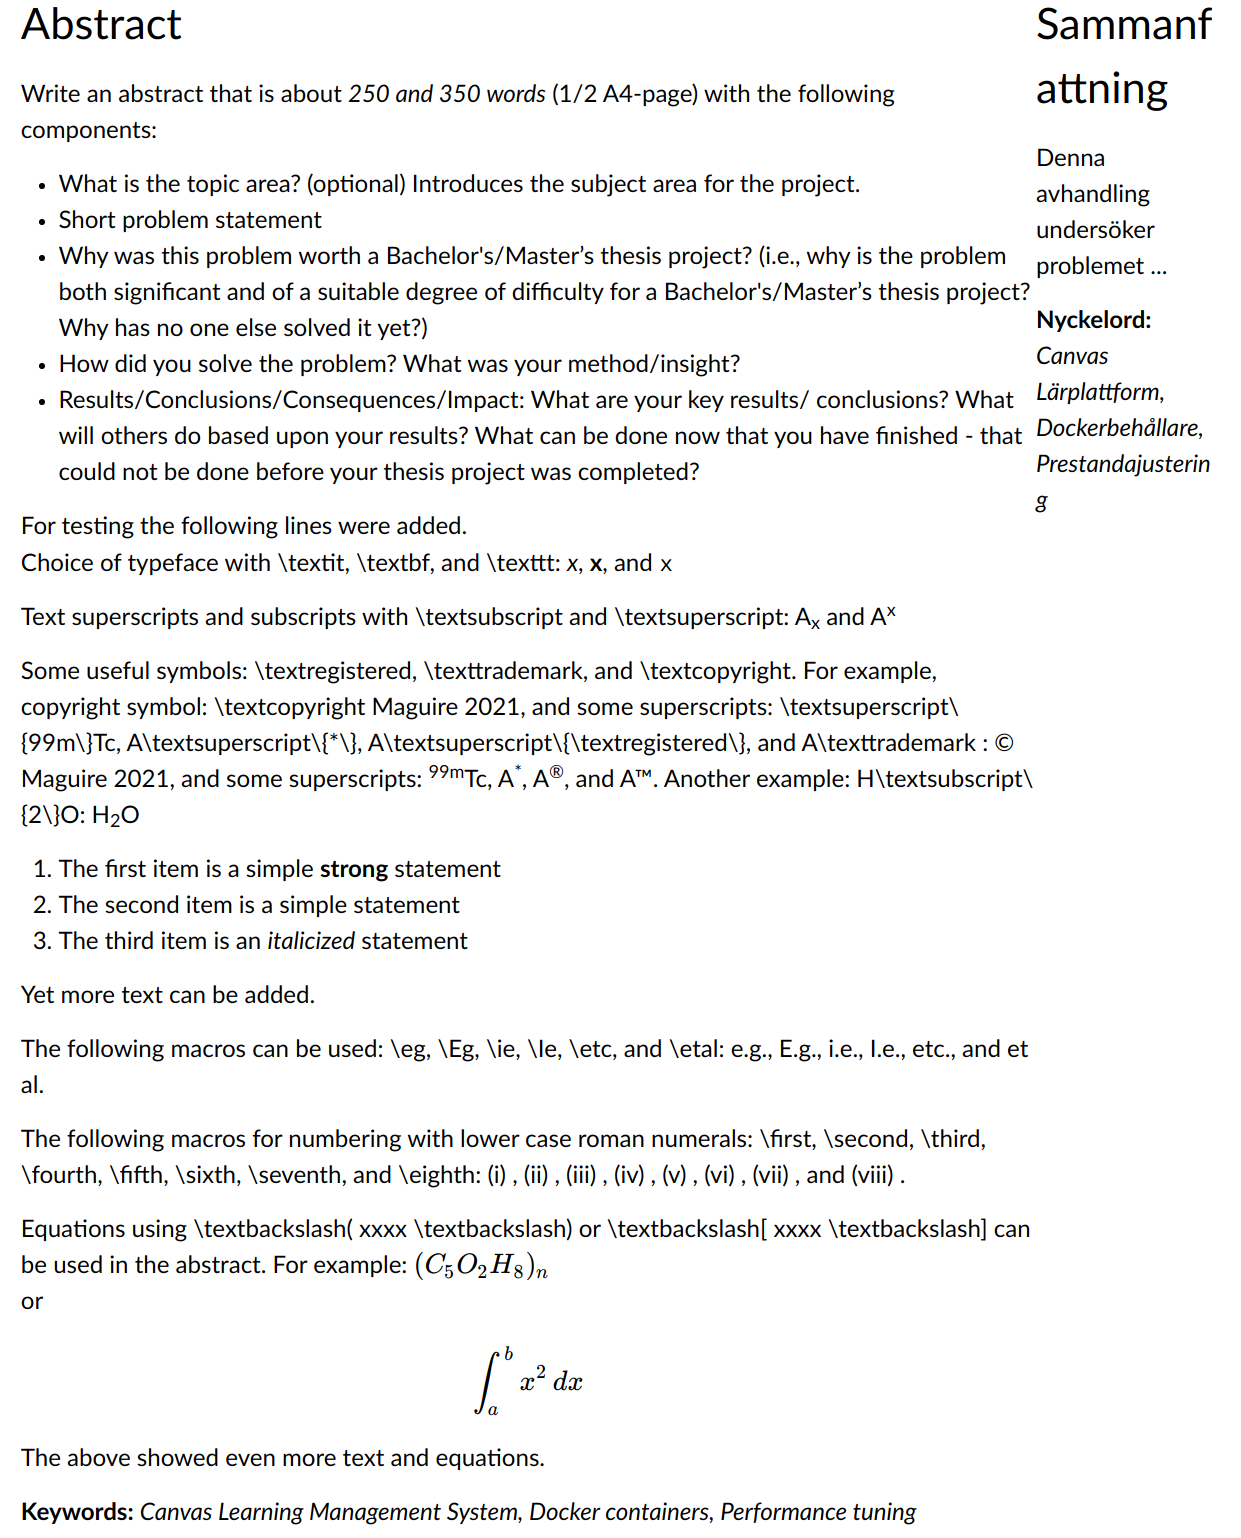
\includegraphics[width=0.5\textwidth]{README_notes/README-examiner-figures/resulting_announcement_109.png}}
  \end{center}
  \caption{Resulting announcement}
  \label{fig:resultingAnnouncementPNG}
\end{figure}
\FloatBarrier


This contrived example shows that a \LaTeX~abstract of the form shown in \Cref{lst:JSONtoLadokK} can be handled. While more testing should be done, this shows that it is possible to directly extract the data that is written to the file as pseudo JSON \LaTeX~\textit{without} having to parse and process the PDF file; however, you still have to compile the \LaTeX~and produce the PDF file in order to produce the \texttt{fordiva.json} file.

\textbf{NB}: that the cleanup\_pseudo\_JSON-from\_LaTeX.py program does simple text substitution and cannot handle nested \LaTeX~commands.

	
\begin{lstlisting}[language={}, caption={Source \LaTeX~(from inside the scontents of the abstract)}, label=lst:JSONtoLadokK]
Write an abstract that is about \textit{250 and 350 words} (1/2 A4-page)  with the following components: % key parts of the abstract
\begin{itemize}
  \item What is the topic area? (optional) Introduces the subject area for the project.
  \item Short problem statement
  \item Why was this problem worth a Bachelor's/Master’s thesis project? (\ie, why is the problem both significant and of a suitable degree of difficulty for a Bachelor's/Master’s thesis project? Why has no one else solved it yet?)
  \item How did you solve the problem? What was your method/insight?
  \item Results/Conclusions/Consequences/Impact: What are your key results/\linebreak[4]conclusions? What will others do based upon your results? What can be done now that you have finished - that could not be done before your thesis project was completed?
\end{itemize}

For testing the following lines were added.
Choice of typeface with \textbackslash textit, \textbackslash textbf, and \textbackslash texttt:  \textit{x}, \textbf{x}, and \texttt{x}

Text superscripts and subscripts with \textbackslash textsubscript and \textbackslash textsuperscript: A\textsubscript{x} and A\textsuperscript{x}

Some useful symbols: \textbackslash textregistered, \textbackslash texttrademark, and \textbackslash textcopyright. For example, copyright symbol: \textbackslash textcopyright Maguire 2021, and some superscripts: \textbackslash textsuperscript\{99m\}Tc, A\textbackslash textsuperscript\{*\}, A\textbackslash textsuperscript\{\textbackslash textregistered\}, and A\textbackslash texttrademark : \textcopyright Maguire 2021, and some superscripts: \textsuperscript{99m}Tc, A\textsuperscript{*}, A\textsuperscript{\textregistered}, and A\texttrademark. Another example: H\textbackslash textsubscript\{2\}O: H\textsubscript{2}O

\begin{enumerate}
  \item The first item is a simple \textbf{strong} statement
  \item The second item is a simple statement
  \item The third item is an \textit{italicized} statement
\end{enumerate}

Yet more text can be added.

The following commands can be used: \textbackslash eg, \textbackslash Eg, \textbackslash ie, \textbackslash Ie, \textbackslash etc, and \textbackslash etal: \eg, \Eg, \ie, \Ie, \etc, and \etal

The following commands for numbering with lower case roman numerals: \textbackslash first, \textbackslash Second, \textbackslash third, \textbackslash fourth, \textbackslash fifth, \textbackslash sixth, \textbackslash seventh, and \textbackslash eighth: \first, \Second, \third, \fourth, \fifth, \sixth, \seventh, and \eighth.

Equations using \textbackslash( xxxx \textbackslash) or \textbackslash[ xxxx \textbackslash] can be used in the abstract. For example: \( (C_5O_2H_8)_n \)
or \[ \int_{a}^{b} x^2 \,dx \]

The above showed even more text and equations.
\end{lstlisting}


The Overleaf project used to workout the string reading and tokenize is at \url{https://www.overleaf.com/read/mqtrxrdcssmg} while the “KTH thesis template for 1\textsuperscript{st} and 2\textsuperscript{nd} cycle degree projects with JSON output” can be found at \url{https://www.overleaf.com/read/gxhwkywbtgsn}.

The reason for adding the reservation “(almost)” in the earlier paragraph was that this file is not directly readable by my programs that could accept the pseudo JSON that I produced with earlier programs. Some of the problems are that the opponents’ name string contains “\&”, \ie it is "A. B. Normal \& A. X. E. Normalè" and this is not acceptable to python’s json.loads{} function; thus, this has to be rewritten. Additionally, the abstracts contain the raw \LaTeX~and thus can include acronyms that need to be spelled out. This means that the same transformations used in \texttt{extract\_pseudo\_JSON-from\_PDF.py} need to be implemented in a new program to clean up the pseudo JSON. This new program is named: \texttt{cleanup\_pseudo\_JSON-from\_LaTeX.py}.

\FloatBarrier

\section{Abstracts in languages that use characters other than those in the main font}
Note that if the user has set the option \texttt{includeExtraAbstracts} and included abstracts that require fonts other than \texttt{TeX Gyre Termes}, the contents of the abstracts in these languages may not appear on the ``For DiVA'' page but will be in the \texttt{fordiva.json} file, unless you add \texttt{\textbackslash newunicodechar} definitions that utilize a font where the characters appearing in the abstract are available.

\begin{listing}[!ht]
\begin{minted}[breaklines, escapeinside=||]{text}
Missing character: There is no 中 (U+4E2D) in font TeX Gyre Cursor/OT:script=latn;language=dflt;-liga;+lnum;+tnum;mapping=tex-text;!
Missing character: There is no 文 (U+6587) in font TeX Gyre Cursor/OT:script=latn;language=dflt;-liga;+lnum;+tnum;mapping=tex-text;!
Missing character: There is no 摘 (U+6458) in font TeX Gyre Cursor/OT:script=latn;language=dflt;-liga;+lnum;+tnum;mapping=tex-text;!
Missing character: There is no 要 (U+8981) in font TeX Gyre Cursor/OT:script=latn;language=dflt;-liga;+lnum;+tnum;mapping=tex-text;!
Missing character: There is no 个 (U+4E2A) in font TeX Gyre Heros/OT:script=latn;language=dflt;mapping=tex-text;!
Missing character: There is no 关 (U+5173) in font TeX Gyre Heros/OT:script=latn;language=dflt;mapping=tex-text;!
Missing character: There is no 键 (U+952E) in font TeX Gyre Heros/OT:script=latn;language=dflt;mapping=tex-text;!
Missing character: There is no 词 (U+8BCD) in font TeX Gyre Heros/OT:script=latn;language=dflt;mapping=tex-text;!
\end{minted}
\caption{Examples of missing characters from the output.log file}
\label{lst:missingCharactersFromLogExample}
\end{listing}

\begin{listing}[!ht]
\begin{minted}[breaklines, escapeinside=||]{text}
\newunicodechar{个}{\iffontchar\font`个 个\else{\cjkfonttt 个}\fi} % U+4E2A - CJK Unified Ideograph-4E2A
\newunicodechar{中}{\iffontchar\font`中 中\else{\cjkfonttt 中}\fi} % U+4E2D - CJK Unified Ideograph-4E2D
\newunicodechar{关}{\iffontchar\font`关 关\else{\cjkfonttt 关}\fi} % U+5173 - CJK Unified Ideograph-5173
\newunicodechar{摘}{\iffontchar\font`摘 摘\else{\cjkfonttt 摘}\fi} % U+6458 - CJK Unified Ideograph-6458
\newunicodechar{文}{\iffontchar\font`文 文\else{\cjkfonttt 文}\fi} % U+6587 - CJK Unified Ideograph-6587
\newunicodechar{要}{\iffontchar\font`要 要\else{\cjkfonttt 要}\fi} % U+8981 - CJK Unified Ideograph-8981
\newunicodechar{词}{\iffontchar\font`词 词\else{\cjkfonttt 词}\fi} % U+8BCD - CJK Unified Ideograph-8BCD
\newunicodechar{键}{\iffontchar\font`键 键\else{\cjkfonttt 键}\fi} % U+952E - CJK Unified Ideograph-952E
\end{minted}
\caption{Examples of new unicode character definitions}
\label{lst:newunicodeForAbstracts}
\end{listing}
\FloatBarrier

%% add more here

\section[Inserting information into LADOK]{Inserting information into LADOK}
\label{sec:JSONtoLADOK}
As part of the effort to be able to minimize the effort of cutting and pasting. I have made a program JSON\_to\_ladok.py that takes the extracted JSON information and uses the information about the author(s) and the title and alternative title to try to insert this information into LADOK for the module (\ie ``moment'' in Swedish) that requires a project title, \ie, 'KravPaProjekttitel' is True. \Cref{lst:usingExtractedJSONtoProduceLADOKentry} shows an example of using this program to try to put the title and alternative title into LADOK. Basically the program logic should work, but I do \textbf{not} have the required permission to make entries of this sort of data for a degree project.

Note that this program uses the \texttt{ladok3} python library but extends it with some features that are not (yet) in the library. It should be regarded as very much a work in progress.
\begin{lstlisting}[language={bash}, caption={Using the extracted JSON to produce a LADOK entry}, label=lst:usingExtractedJSONtoProduceLADOKentry]
./JSON_to_ladok.py -c 11   --json xxx.json   --code DA213X
testing=False
d={'Author1': {'Last name': ‘xxx’, 'First name': 'xxx', 'Local User Id': 'yyyyy', 'E-mail': 'xxx@kth.se', 'organisation': {'L1': 'School of EXXX'}}, 'Degree': {'Educational program': 'Master’s Programme, XXX, 120 credits', 'programcode': 'TXXXX', 'Level': '2', 'Course code': 'XX200X', 'Credits': '30.0', 'Exam': 'Master’s Programme, XXX, 120 credits', 'subjectArea': 'XXX'}, 'Title': {'Main title': 'xxx', 'Subtitle': yyyy', 'Language': 'eng'}, 'Alternative title': {'Main title': 'zzzz', 'Subtitle': wwwww', 'Language': 'swe'}, 'Supervisor1': {'Last name': 'x', 'First name': 'y', 'Local User Id': 'xx', 'E-mail': 'xxxxx@kth.se', 'organisation': {'L1': 'School of XXX', 'L2': 'DepartmentName'}}, 'Supervisor2': {'Last name': 'yyy', 'First name': 'xxx', 'E-mail': 'xxx@zzzz.com', 'Other organisation': ‘zzzz'}, 'Examiner1': {'Last name': 'ExaminersLastname', 'First name': 'ExaminersFirstname', 'Local User Id': 'u1000000', 'E-mail': 'XXX@kth.se', 'organisation': {'L1': 'School of XXX', 'L2': 'DepartmentName'}}, 'Cooperation': {'Partner_name': 'xxx'}, 'National Subject Categories': '10201, 10206', 'Other information': {'Year': '2021', 'Number of pages': 'xix,99'}, 'Opponents': {'Name': 'A. B. Normal & A. X. E. Normalè'}, 'Presentation': {'Date': '2021-03-15 13:00', 'Language': 'eng', 'Room': 'via Zoom', 'Address': 'Isafjordsgatan 22 (Kistagången 16)', 'City': 'Stockholm'}, 'Number of lang instances': '2', 'abstracts': {'eng': xxxx", 'swe': 'yyyy'}, 'keywords': {'eng': 'x, y z', 'swe': x, y, z'}}
course_code=DA231X
author={'Last name': 'xxx', 'First name': 'yyy', 'Local User Id': 'u1xxxx', 'E-mail': 'oxxx@kth.se', 'organisation': {'L1': 'School of XXX'}}
sortable name=X,Y
Canvas user_id=dddd
integration_id=gggggg-gggg-gggg-gggg-ggggggg
ladoK_course_info={'id': 'gggggggg-gggg-gggg-gggg-gggggggggggg', 'round_id': 'gggggggg-gggg-gggg-gggg-gggggggggggg', 'education_id': 'gggggggg-gggg-gggg-gggg-gggggggggggg', 'instance_id': 'gggggggg-gggg-gggg-gggg-gggggggggggg', 'swe_name': 'Examensarbete i XXX, avancerad nivå', 'eng_name': 'Degree Project in XXX, Second Cycle'}
moment code=PRO1, requires title=False
moment code=PRO2, requires title=False
moment code=PRO3, requires title=True
trying to store a passing grade for moment=PRO3
Traceback (most recent call last):
  File "./JSON_to_ladok.py", line 533, in <module>
    sys.exit(main(sys.argv[1:]))
  File "./JSON_to_ ladok.py", line 519, in main
    status=save_result_degree_project3(ladok, integration_id, course_code, mom['Utbildningskod'], '2021-07-14', 'P', "PF", main_title, alternative_main_title)
  File "./JSON_to_ ladok.py", line 374, in save_result_degree_project3
    raise Exception("Couldn't register " + course_moment + "=" + grade_raw + " " + result_date_raw + ": " + r.json()["Meddelande"])
Exception: Couldn't register PRO3=P 2021-07-14: Hinder mot skapa resultat påträffat: Rapporteringsrättighet saknas
\end{lstlisting}


\section{Removing the README\_examiner\_notes}
At some point you will no longer want this README information. You can remove it by removing the line
\textbackslash include\{README\_notes/README\_examiner\_notes\} -- from the \texttt{examplethesis.tex} file. You can then remove the \texttt{README\_notes} directory.

\section[Copyright or Creative Commons License]{Copyright or Creative Commons\\ License}
\label{sec:copyrightOrCClicenseExaminer}
It is possible to have several variants of the bookinfo page:
\begin{enumerate}[labelwidth =\widthof{\textbf{Creative Commons (CC)}}, leftmargin = !]
    \item[copyright] If you want to have a bookinfo page, include the line saying \texttt{\textbackslash bookinfopage}.
    \item[Creative Commons (CC)] If you want to have a bookinfo page but want to have a Creative Commons license, then include \texttt{\textbackslash bookinfopage} and use and configure the \texttt{doclicense} package as shown in Listings \ref{lst:CCBY-NC-ND}, \ref{lst:CCBY-NC-ND-euro}, and \ref{lst:CCzero}.
    \item[none] If you do \textbf{not} want to have a bookinfo page, comment the line saying \texttt{\textbackslash bookinfopage} and add a \texttt{\textbackslash cleardoublepage}.
\end{enumerate}

For background about Creative Commons licenses see:
\url{https://www.kb.se/samverkan-och-utveckling/oppen-tillgang-och-bibsamkonsortiet/open-access-and-bibsam-consortium/open-access/creative-commons-faq-for-researchers.html} and \url{https://kib.ki.se/en/publish-analyse/publish-your-article-open-access/open-licence-your-publication-cc}.

Note that the lowercase version of the license has to be used in the modifier, \ie one of: by, by-nc, by-nd, by-nc-nd, by-sa, by-nc-sa, or zero. For the list of supported licenses see the documentation for the \texttt{doclicense} package.

\begin{lstlisting}[language={[LaTeX]TeX}, caption={Example configuration to have a CC BY-NC-ND license}, label=lst:CCBY-NC-ND]
\usepackage[
    type={CC},
    modifier={by-nc-nd},
    version={4.0},
    hyphenation={RaggedRight},
]{doclicense}
\end{lstlisting}

Note that the option ``hyphenation={RaggedRight}'' can be used with the configuration of the package to set the license information with a ragged right margin rather that as a fill and justified paragraph.

\begin{lstlisting}[language={[LaTeX]TeX}, caption={Example configuration to have a CC BY-NC-ND license with a Euro symbol rather than a Dollar sign}, label=lst:CCBY-NC-ND-euro]
\usepackage[
    type={CC},
    modifier={by-nc-nd},
    version={4.0},
    imagemodifier={-eu-88x31},  % to get Euro symbol rather than Dollar sign
    hyphenation={RaggedRight},
]{doclicense}
\end{lstlisting}

\begin{lstlisting}[language={[LaTeX]TeX}, caption={Example configuration to have a CC0 license}, label=lst:CCzero]
\usepackage[
    type={CC},
    modifier={zero},
    version={1.0},
]{doclicense}
\end{lstlisting}


For someone who is maintaining or modifying the template, it is important to know that the \texttt{\textbackslash bookinfopageCC} command has a case statement in it that uses an internal variable (\texttt{\textbackslash doclicense@modifier}) set by \texttt{doclicense} as shown in~\Cref{lst:bookinfopageCCcaseSTMT}. This case statement will need to be modified if there is a change in the set of Creative Commons licenses. While it might be possible to replace this case statement with \texttt{\textbackslash doclicenseModifier} to directly produce the capitalized version of the license names or perhaps even \texttt{\textbackslash doclicenseName} or \texttt{\textbackslash doclicenseNameRef} to include the capitalized license name as well as the version number (the later also including a URL to the license). However, I think that these alternatives are unnecessary give the \texttt{\textbackslash doclicenseThis} that generates the display of the license with logo(s). More importantly, using these other commands rather than the unprocessed \texttt{\textbackslash doclicense@modifier} lads to problems when writing out the \texttt{fordiva.json} file.

Note that if the \texttt{doclicense} package is used it automatically redefines \texttt{\textbackslash bookinfopage} to be \texttt{\textbackslash bookinfopageCC}.

\begin{lstlisting}[language={[LaTeX]TeX}, caption={Case statement in \textbackslash bookinfopageCC}, label=lst:bookinfopageCCcaseSTMT]
  \IfEqCase{\doclicense@modifier}{%
    {by}{CC BY}%
    {by-nc}{CC BY-NC}%
    {by-nd}{CC BY-ND}%
    {by-nc-nd}{CC BY-NC-ND}%
    {by-sa}{CC BY-SA}%
    {by-nc-sa}{CC BY-NC-SA}%
    {zero}{CC0}%
  }[\typeout{Creative Commons code  \doclicense@modifier not found}\copyright]
\end{lstlisting}

There is a new \texttt{\textbackslash thesiscopyrightleft} command added to the \texttt{\textbackslash bookinfopage} and \texttt{\textbackslash bookinfopageCC} pages to store the value of the copyright or copyleft information that the user chose (if any). This information is later output as information for DiVA in the form shown in \Cref{lst:bookinfoCopyrightselected,lst:bookinfoCopyleftselected,lst:bookinfoNoneselected}
\begin{lstlisting}[language=json, caption={If the user chose to have a copyright on the bookinfo page}, label=lst:bookinfoCopyrightselected]
"Copyrightleft": "copyright"
\end{lstlisting}

\begin{lstlisting}[language=json, caption={If the user chose to have a CC BY-NC license on the bookinfo page}, label=lst:bookinfoCopyleftselected]
"Copyrightleft": "by-nc"
\end{lstlisting}

\begin{lstlisting}[language=json, caption={If the user chose \textbf{not} to have a bookinfo page}, label=lst:bookinfoNoneselected]
"Copyrightleft": "None"
\end{lstlisting}

As a result of adding support for the PDF metadata for the copyright, the template now uses the \texttt{hyperxmp} package. Details of the code to set the value of the pdfcopyright metadata can be seen in \Cref{lst:bookinfopageCopyrightPDFmetadata}.
The use of \texttt{hyperxmp} caused a change in how the author's name is processed - for details about this see \Cref{sec:addingKeywordsAndMetaDataToPDF} starting on page~\pageref{sec:addingKeywordsAndMetaDataToPDF}.

\begin{lstlisting}[language={[LaTeX]TeX}, caption={Processing copyright PDF metadata information in \textbackslash bookinfopageCC}, label=lst:bookinfopageCopyrightPDFmetadata]
% Command to print out the standardized document information page
\newcommand{\bookinfopage}{
\ifgfivepaper
  \newgeometry{top=140mm,bottom=30mm,left=12.25mm,right=35mm}
\else
  \newgeometry{top=250mm,bottom=30mm,left=74pt,right=35mm}
\fi
\thispagestyle{empty}
\begin{flushleft}
  \sffamily
  \copyright\enspace\the\year\quad\@authorsFirstname\space\@authorsLastname 
  \ifx\@secondAuthorsLastname\@empty\relax
  \else
    \ifinswedish
      \enspace och\enspace\@secondAuthorsFirstname\space\@secondAuthorsLastname \\
    \else
      \enspace and\enspace\@secondAuthorsFirstname\space\@secondAuthorsLastname \\
    \fi
  \fi
\end{flushleft}
\thesiscopyrightleft{copyright}
\newcommand{\mycopyright}{%
  {Copyright (c)}\ \the\year\ \@authorsFirstname\ \@authorsLastname %
  \ifx\@secondAuthorsLastname\@empty\relax%
  \else%
    \ifinswedish%
      \  och\ \@secondAuthorsFirstname\ \@secondAuthorsLastname%
    \else%
      \  and\ \@secondAuthorsFirstname\ \@secondAuthorsLastname%
    \fi%
  \fi%
}
\hypersetup{
     pdfcopyright={\mycopyright} 
}
\restoregeometry
\clearpage
}

% bookinfo page with CC license
% CC BY (Attribution)
% CC BY-NC (Attribution + Non-commercial)
% CC BY-ND (Attribution + No derivatives)
% CC BY-NC-ND (Attribution + Non-commercial + No derivatives)
% CC BY-SA (Attribution + ShareAlike)
% CC BY-NC-SA (Attribution + Non-commercial + ShareAlike)
% CC0 (Zero)
\newcommand{\bookinfopageCC}{
\ifgfivepaper
  \newgeometry{top=130mm,bottom=30mm,left=12.25mm,right=35mm}
\else
  \newgeometry{top=220mm,bottom=30mm,left=74pt,right=35mm}
\fi
\thispagestyle{empty}
\begin{flushleft}
  \sffamily
  \IfEqCase{\doclicense@modifier}{%
    {by}{CC BY}%
    {by-nc}{CC BY-NC}%
    {by-nd}{CC BY-ND}%
    {by-nc-nd}{CC BY-NC-ND}%
    {by-sa}{CC BY-SA}%
    {by-nc-sa}{CC BY-NC-SA}%
    {zero}{CC0}%
  }[\typeout{Creative Commons code  \doclicense@modifier not found}\copyright]
  \enspace\the\year\quad\@authorsFirstname\space\@authorsLastname 
  \ifx\@secondAuthorsLastname\@empty\relax
  \else
    \ifinswedish
      \enspace och\enspace\@secondAuthorsFirstname\space\@secondAuthorsLastname \\
    \else
      \enspace and\enspace\@secondAuthorsFirstname\space\@secondAuthorsLastname \\
    \fi
  \fi
  \doclicenseThis
\end{flushleft}
\thesiscopyrightleft{\doclicense@modifier}

\let\@myCC\@empty
\ifdefstring{\doclicense@modifier}{by}{\def\@myCC{CC BY}}
\ifdefstring{\doclicense@modifier}{by-nc}{\def\@myCC{CC BY-NC}}
\ifdefstring{\doclicense@modifier}{by-nd}{\def\@myCC{CC BY-ND}}
\ifdefstring{\doclicense@modifier}{by-nc-nd}{\def\@myCC{CC BY-NC-ND}}
\ifdefstring{\doclicense@modifier}{by-sa}{\def\@myCC{CC BY-SA}}
\ifdefstring{\doclicense@modifier}{by-nc-sa}{\def\@myCC{CC BY-NC-SA}}
\ifdefstring{\doclicense@modifier}{zero}{\def\@myCC{CC0}}

\newcommand{\mycopyright}{%
 \@myCC\ \the\year\ \@authorsFirstname\ \@authorsLastname%
  \ifx\@secondAuthorsLastname\@empty\relax%
  \else%
    \ifinswedish%
      \  och\ \@secondAuthorsFirstname\ \@secondAuthorsLastname%
    \else%
      \ and\ \@secondAuthorsFirstname\ \@secondAuthorsLastname %
    \fi%
  \fi%
}

\hypersetup{
     pdfcopyright={\mycopyright} 
}
\restoregeometry
\clearpage
}

% If the doclicense pacakage is installed, then use the \bookinfoCC when encountering a \bookinfo command
\AtBeginDocument{\@ifpackageloaded{doclicense}
  {%
    \renewcommand{\bookinfopage}{\bookinfopageCC}
  }
  {\relax}
}
\end{lstlisting}

\section[Adding acronyms.tex to For DIVA info]{Adding acronyms.tex to For DIVA info}
\label{sec:acronymsInForDIVAdata}
If the author has used acronyms in the abstract(s), then these acronym definitions need to be available in some way to the person (or program) that makes the MODS file. One solution is to add them at the end of the For DIVA information. This can be done using the code shown in~\Cref{lst:includeAcronymsFile}. This code simply checks for the file and if it is present appends the contents of this file to the text as a listing. An important part to note is the option \texttt{nolol} - this prevents this listing from appearing in the list of listings.

\begin{lstlisting}[language={[LaTeX]TeX}, caption={Code for adding acronyms.tex at the end of the For DIVA data}, label=lst:includeAcronymsFile]
% If there is an acronyms.tex file,
% add it to the end of the For DIVA information
% so that it can be used with the abstracts
% Note that the option "nolol" stops it from being listed in the List of Listings
\IfFileExists{lib/acronyms.tex}{
\section*{acronyms.tex}
\lstinputlisting[language={[LaTeX]TeX}, nolol, basicstyle=\ttfamily\color{black},
commentstyle=\color{black}, backgroundcolor=\color{white}]{lib/acronyms.tex}
}
{}
\end{lstlisting}

\section{Adding additional metadata to the PDF file}
\label{sec:addingMetadataToPDFfile}
It is increasingly the case that metadata is being embedded into digital objects to provide information about the creator (author, photographer, \etc), date of creation, copyright notices, \etc. In a typical PDF file produced by \LaTeX~there is both PDF-specific metadata and additional metadata. This additional metadata is stored using Adobe's Extensible Metadata Platform (XMP). XMP is a means of embedding metadata in XML format into PDF documents so that tools can extract it mechanically.

An early paper about automatically extracting the title, authors(s), and abstract from theses was written by Mao Ni of the University of North Carolina at Chapel Hill, School of Library and Information Science in 2004\,\cite{Mao_Ni_2004}. The idea was to collect the metadata from the thesis using an Adobe Acrobat plugin and then write this data to XMP (which could be embedded into the PDF file). The schema used for the metadata\cite{hickey_pavani_suleman_2010} \footnote{\url{https://ndltd.org/metadata/}} was that of Networked Digital Library of Theses and Dissertations\footnote{\url{https://ndltd.org/}}.

More recently, Elsevier's Digital Commons \footnote{\url{https://www.elsevier.com/solutions/digital-commons}} uses an extension of the Dublin Core\footnote{\url{https://www.dublincore.org/}} shown in \Cref{tab:dublicCoreDigitalCommons} to collect metadata. We will see the Dublin Core elements and others metadata schema used in XMP in the remainder of this section.

Bepress has written about Elsevier's Digital Commons in a webpage ``Digital Commons and OAI-PMH: Outbound Harvesting of Repository Records'' \url{https://bepress.com/reference_guide_dc/digital-commons-oai-harvesting/}. The Open Archives Initiative Protocol for Metadata Harvesting (OAI-PMH) is to foster interoperability between repositories\footnote{\url{https://www.openarchives.org/pmh/}} to enable harvesters to collect metadata from a repository. Over the last 20 years there has been an evolution from simply having metadata in a database that is associated with a publication to an entire ecosystem of metadata and applications - see for example, the twentieth International Conference on Dublin Core and Metadata Applications (DCMI 2022) - \url{https://www.dublincore.org/conferences/2022/programme/}.
\clearpage

\begin{table}[!ht]
    \caption{Dublin Core Elements in Digital Commons\cite{digital_commons_metadata_2016} - items in bold are from the so-called ``simple Dublic Core''}
    \label{tab:dublicCoreDigitalCommons}
    \begin{footnotesize}   
    \begin{tabular}{l | l }
      \textbf{Element} & \textbf{Element} \\
      \hline
\textbf{dc.contributor} & \textbf{dc.rights}\\
dc.contributor.role & dc.rights.accessRights\\
\textbf{dc.coverage} & dc.rights.license\\
dc.coverage.spatial & \textbf{dc.source}\\
dc.coverage.spatial.lat & \textbf{dc.subject}\\
dc.coverage.spatial.long & \textbf{dc.title}\\
dc.coverage.temporal & dc.title.alternative\\
\textbf{dc.creator} & \textbf{dc.type}\\
\textbf{dc.date} & dcam.memberOf\\
dc.date.available & dcterms.accrualMethod\\
dc.date.created & dcterms.accrualPeriodicity\\
dc.date.dateAccepted & dcterms.accrualPolicy\\
dc.date.dateCopyrighted & dcterms.audience\\
dc.date.dateSubmitted & dcterms.audience.educationLevel\\
dc.date.issued & dcterms.audience.mediator\\
dc.date.modified & dcterms.instructionalMethod\\
dc.date.valid & dcterms.provenance\\
\textbf{dc.description} & dcterms.rightsHolder\\
dc.description.abstract & geo.alt\\
dc.description.note & thesis.degree\\
dc.description.release & thesis.degree.discipline\\
dc.description.tableOfContents & thesis.degree.grantor\\
\textbf{dc.format} & thesis.degree.level\\
dc.format.extent & thesis.degree.name\\
dc.format.medium\\
\textbf{dc.identifier}\\
dc.identifier.bibliographicCitation\\
\textbf{dc.language}\\
\textbf{dc.publisher}\\
\textbf{dc.relation}\\
dc.relation.conformsTo\\
dc.relation.hasFormat\\
dc.relation.hasPart\\
dc.relation.hasVersion\\
dc.relation.isFormatOf\\
dc.relation.isPartOf\\
dc.relation.isReferencedBy\\
dc.relation.isReplacedBy\\
dc.relation.isRequiredBy\\
dc.relation.isVersionOf\\
dc.relation.references\\
dc.relation.replaces\\
dc.relation.requires\\
\end{tabular}
\end{footnotesize}
\end{table}
\FloatBarrier
\clearpage

\Cref{fig:fileProperties} shows the properties of a PDF file when using an old version of Adobe Acrobat with the command: File->Properties. This figure shows the Title, Author, Subject, and Keyword fields (among other properties of this PDF file). Because this file was generated in PDF 2.0 format, Acrobat says that you cannot edit the information, and it indicates this by displaying the information in gray.
\begin{figure}[!ht]
  \begin{center}
    \fbox{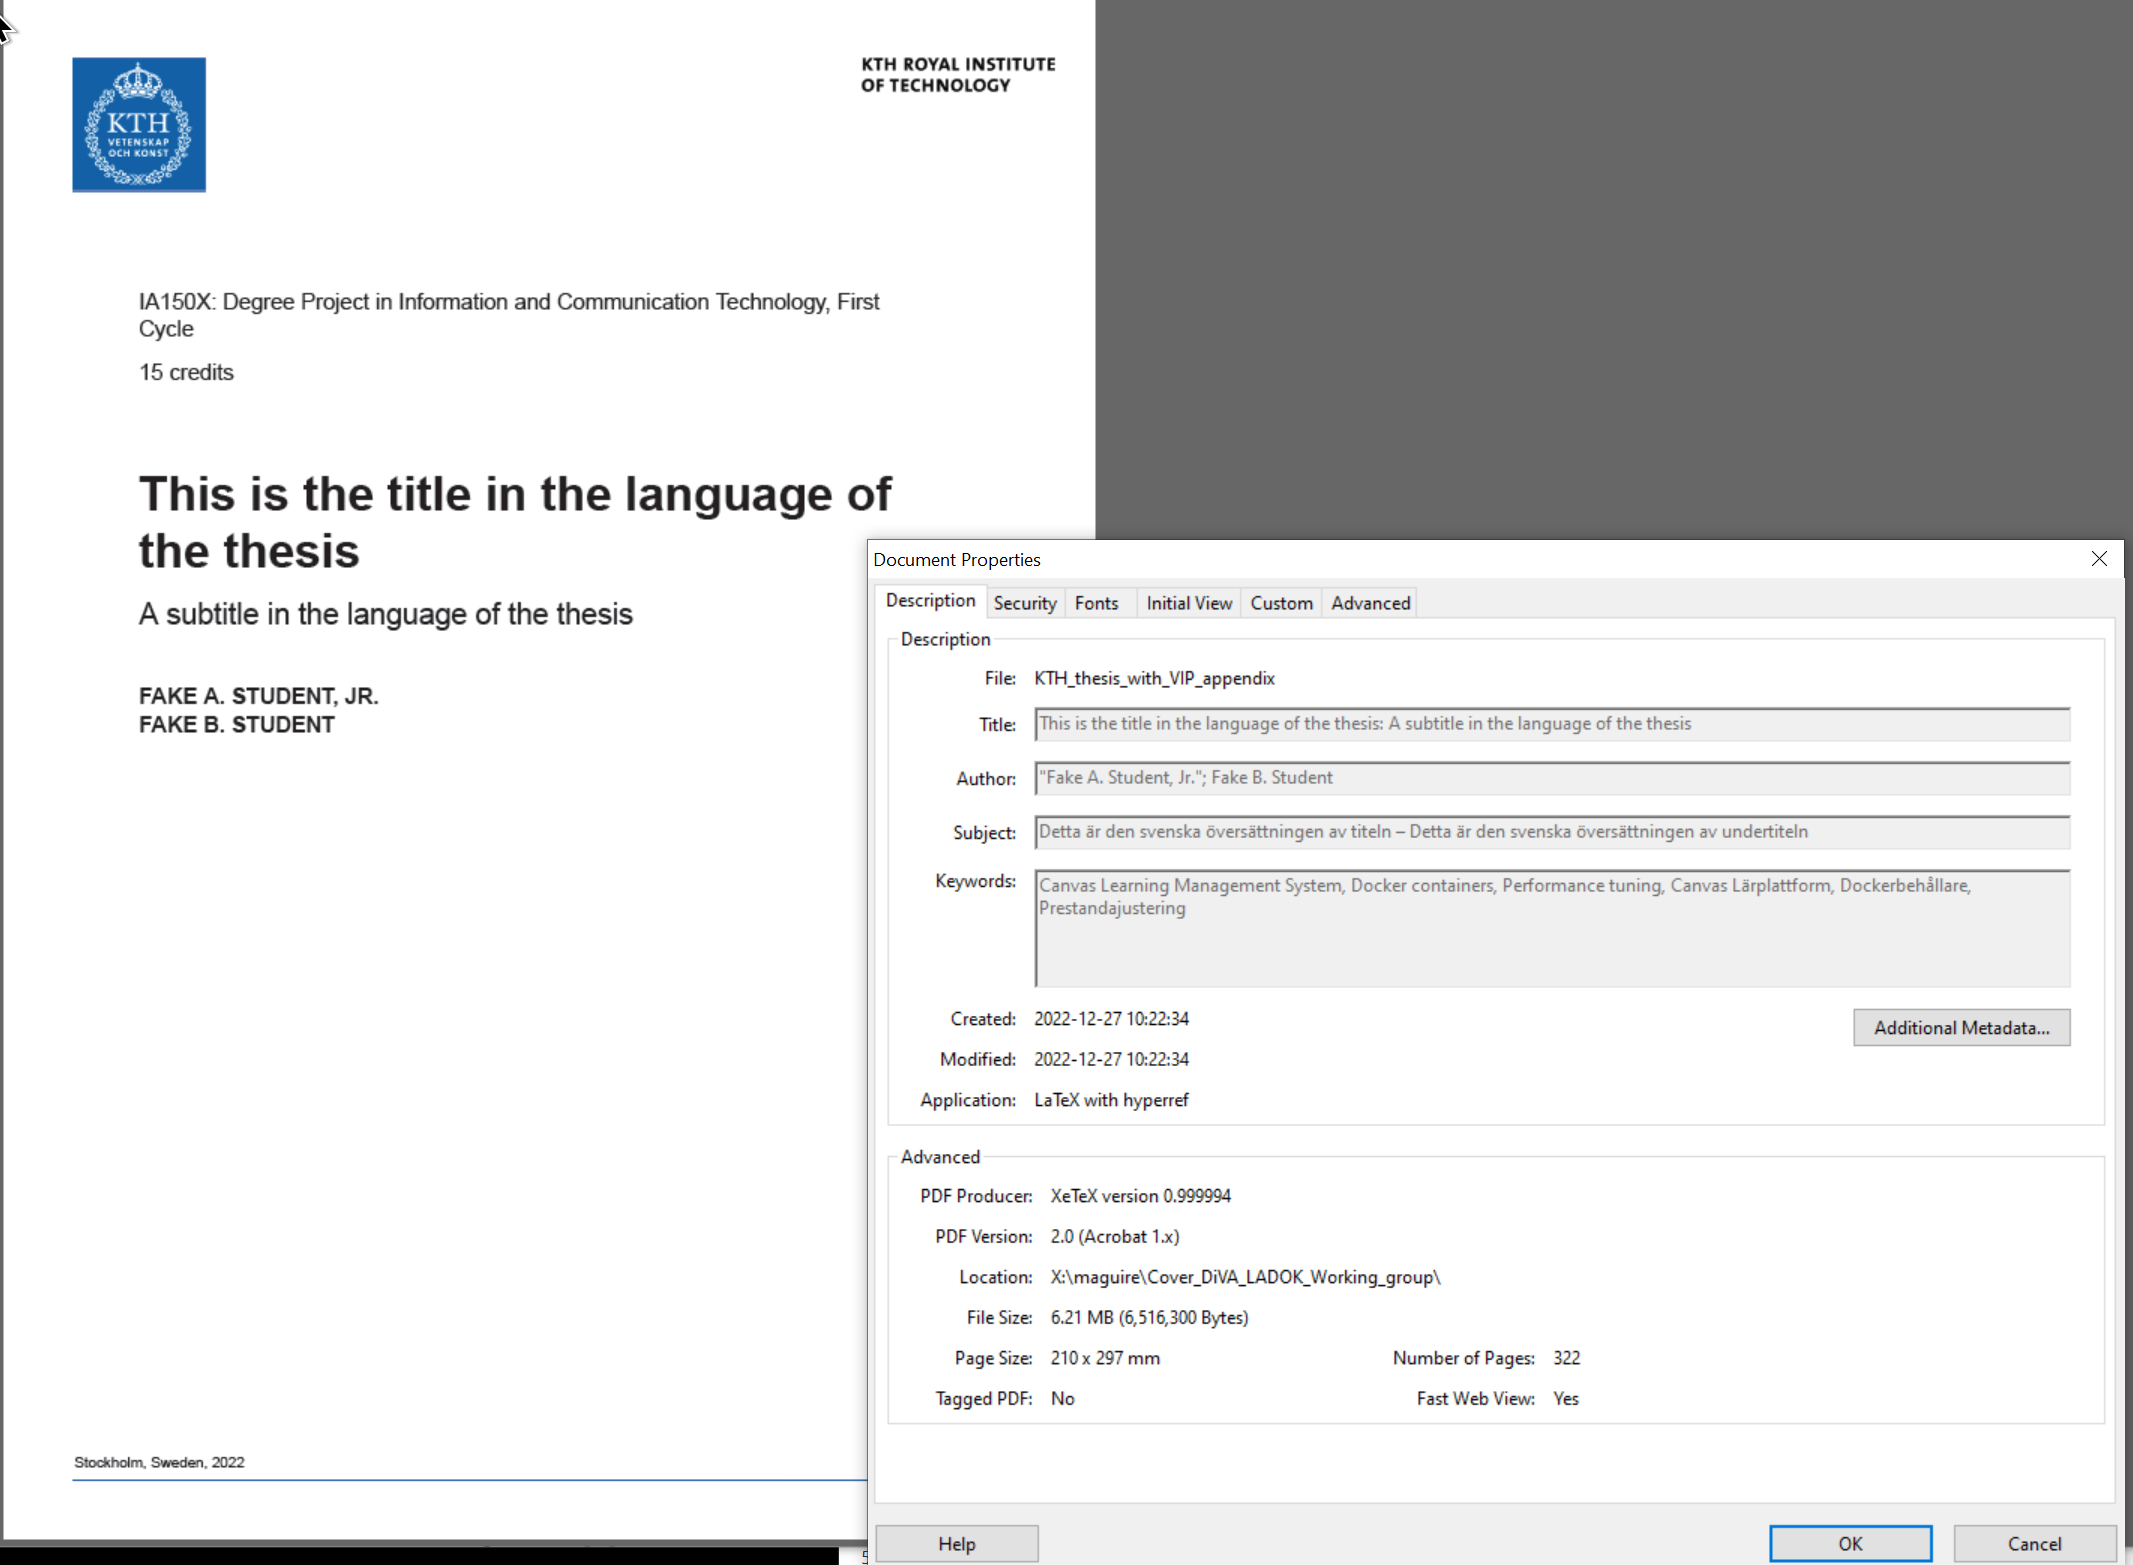
\includegraphics[width=0.9\textwidth]{README_notes/README-examiner-figures/New_thesis_template_document_properties-Screenshot_20221227_115745.png}}
  \end{center}
  \caption{PDF file properties}
  \label{fig:fileProperties}
\end{figure}
\FloatBarrier

\Cref{fig:fileProperties2} shows similar data for another PDF file generated with an earlier PDF version. Because this PDF file uses PDF-1.5, Acrobat displays the information in dark letters, and it is possible to edit the metadata using Acrobat.
\begin{figure}[!ht]
  \begin{center}
    \fbox{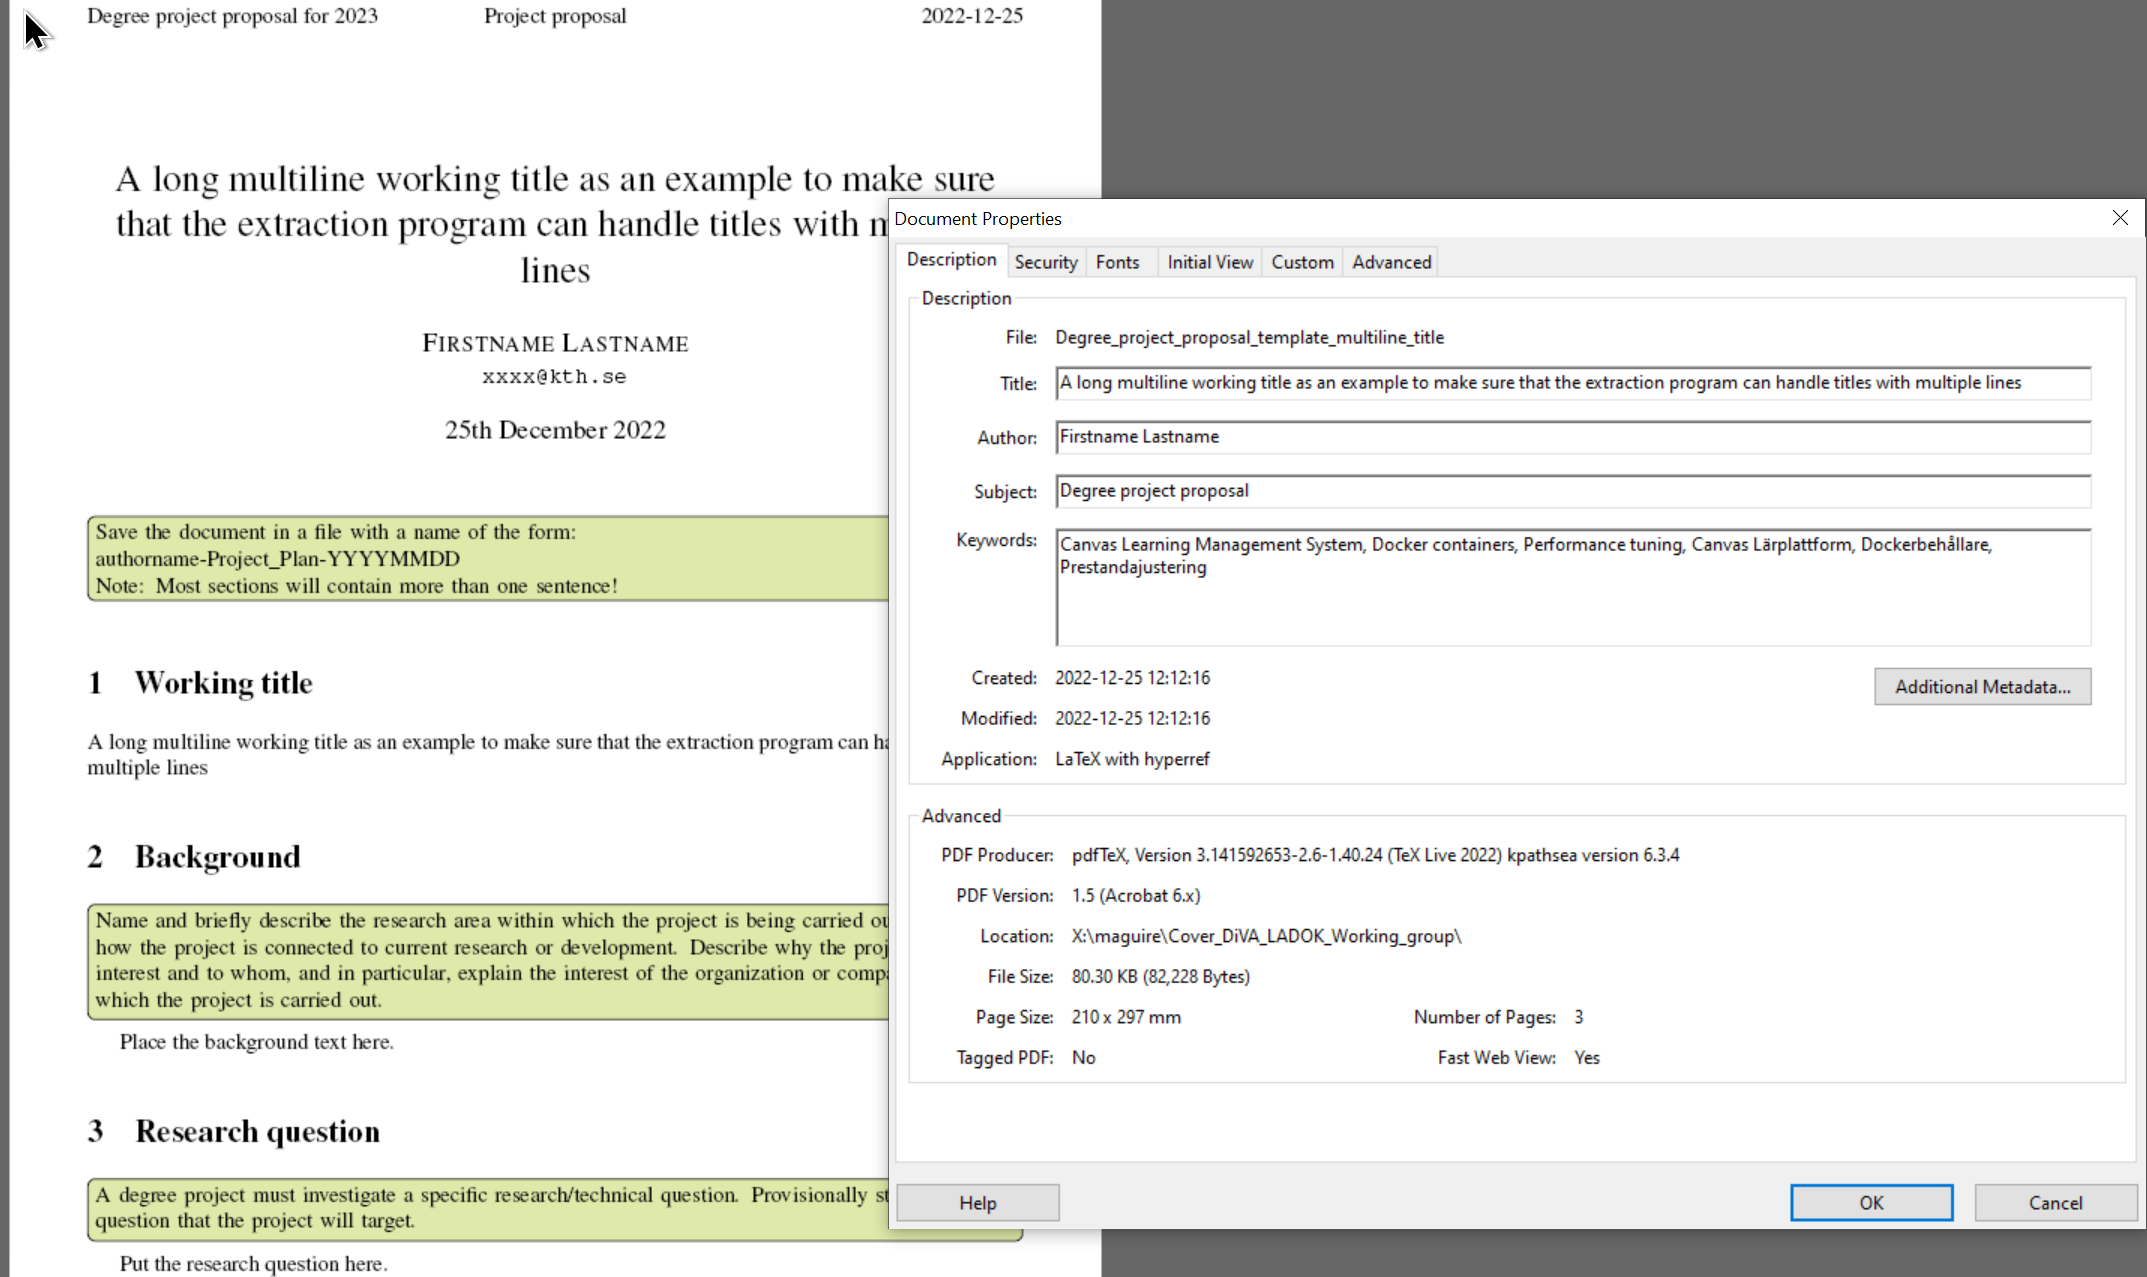
\includegraphics[width=0.9\textwidth]{README_notes/README-examiner-figures/File-properties-Screenshot_20221225_135914.png}}
  \end{center}
  \caption{PDF file properties of another PDF file, in this case, the proposal template}
  \label{fig:fileProperties2}
\end{figure}
\FloatBarrier

The XMP data is in a stream indicated in the PDF as Metadata of the subtype XML, as shown in \Cref{lst:pdfXMPStream}. In the listing, the actual length in bytes has been replaced by dddd.
\begin{lstlisting}[caption={PDF stream where the XMP is found}, label=lst:pdfXMPStream]
<< /Subtype /XML /Type /Metadata /Length dddd >>
stream
\end{lstlisting}

In the PDF file, the XML encoded metadata is between \texttt{<?xpacket begin="yyyy" id="xxxx"?>} and \texttt{<?xpacket end="w"?>} (where xxxx is some unique ID). It is important to note that the value for yyyy in the previous is a so-called byte order marker (BOM) with the value 0xfeff. While this character is a valid \mbox{UTF-8} character, the \texttt{lstlisting} environment cannot handle this value; therefore, it has been replaced by the string ``BOM 0xfeff''. An example of this is shown in \Cref{lst:pdfinfoOutput}.
\clearpage
\begin{lstlisting}[style=myXML,
caption={First part of the XML metadata embedded in a PDF file (some reformatting has been done to fit the text in the boarders)}, label={lst:pdfinfoOutput}]
<?xpacket begin="" id="W5M0MpCehiHzreSzNTczkc9d"?>
<x:xmpmeta xmlns:x="adobe:ns:meta/">
  <rdf:RDF xmlns:rdf="http://www.w3.org/1999/02/22-rdf-syntax-ns#">
    <rdf:Description rdf:about=""
     xmlns:pdf="http://ns.adobe.com/pdf/1.3/"
     xmlns:xmpRights="http://ns.adobe.com/xap/1.0/rights/"
     xmlns:dc="http://purl.org/dc/elements/1.1/"
     xmlns:photoshop="http://ns.adobe.com/photoshop/1.0/"
     xmlns:xmp="http://ns.adobe.com/xap/1.0/"
     xmlns:xmpMM="http://ns.adobe.com/xap/1.0/mm/"
     xmlns:stEvt="http://ns.adobe.com/xap/1.0/sType/ResourceEvent#"
     xmlns:pdfaid="http://www.aiim.org/pdfa/ns/id/"
     xmlns:pdfuaid="http://www.aiim.org/pdfua/ns/id/"
     xmlns:pdfx="http://ns.adobe.com/pdfx/1.3/"
     xmlns:pdfxid="http://www.npes.org/pdfx/ns/id/"
     xmlns:prism="http://prismstandard.org/namespaces/basic/3.0/"
     xmlns:jav="http://www.niso.org/schemas/jav/1.0/"
     xmlns:xmpTPg="http://ns.adobe.com/xap/1.0/t/pg/"
     xmlns:stFnt="http://ns.adobe.com/xap/1.0/sType/Font#"
     xmlns:Iptc4xmpCore="http://iptc.org/std/Iptc4xmpCore/1.0/£\break{\ensuremath{\color{red}\hookrightarrow\space}}£xmlns/"
     xmlns:pdfaExtension="http://www.aiim.org/pdfa/ns/extension/"
     xmlns:pdfaSchema="http://www.aiim.org/pdfa/ns/schema#"
     xmlns:pdfaProperty="http://www.aiim.org/pdfa/ns/property#"
     xmlns:pdfaType="http://www.aiim.org/pdfa/ns/type#"
     xmlns:pdfaField="http://www.aiim.org/pdfa/ns/field#">
\end{lstlisting}

Some of these XML elements include "rdf" elements referring to the Resource Description Framework (RDF)\footnote{\url{https://www.w3.org/RDF/}}.

The XMP data utilizes a number of different schema and namespaces. These namespaces are shown as ``xmlns:xxxx''  in \Cref{lst:pdfinfoOutput}. One namespace is \texttt{xmlns:dc} and this refers to the scheme is `Dublin Core'' \footnote{see Dublin Core Metadata Initiative \url{https://www.dublincore.org/}}. The information about this namespace can be found at \url{http://purl.org/dc/elements/1.1/}. Each of the schema and namespace are described in the next part of the XML, see \Cref{lst:pdfinfoOutputPart2}.

\begin{lstlisting}[style=myXML,
caption={Second part of the XML metadata embedded in a PDF file (some reformatting has been done to fit the text in the boarders)}, label={lst:pdfinfoOutputPart2}]
£$\ldots$ {\color{red} continuation of the above listing}£ 
      <pdfaExtension:schemas>
        <rdf:Bag>
          <rdf:li rdf:parseType="Resource">
            <pdfaSchema:schema>Adobe PDF Schema</pdfaSchema:schema>
            <pdfaSchema:prefix>pdf</pdfaSchema:prefix>
            <pdfaSchema:namespaceURI>http://ns.adobe.com/pdf/1.3/£\break{\ensuremath{\color{red}\hookrightarrow\space}}£</pdfaSchema:namespaceURI>
            <pdfaSchema:property>
              <rdf:Seq>
                <rdf:li rdf:parseType="Resource">
                  <pdfaProperty:name>Trapped</pdfaProperty:name>
                  <pdfaProperty:valueType>Text</pdfaProperty:valueType>
                  <pdfaProperty:category>internal</pdfaProperty:category>
                  <pdfaProperty:description>Indication if the document has been modified to include trapping information</pdfaProperty:description>
                </rdf:li>
              </rdf:Seq>
            </pdfaSchema:property>
          </rdf:li>
          <rdf:li rdf:parseType="Resource">
            <pdfaSchema:schema>XMP Media Management Schema</pdfaSchema:schema>
            <pdfaSchema:prefix>xmpMM</pdfaSchema:prefix>
            <pdfaSchema:namespaceURI>http://ns.adobe.com/xap/1.0/mm/£\break{\ensuremath{\color{red}\hookrightarrow\space}}£</pdfaSchema:namespaceURI>
            <pdfaSchema:property>
              <rdf:Seq>
                <rdf:li rdf:parseType="Resource">
                  <pdfaProperty:name>DocumentID</pdfaProperty:name>
                  <pdfaProperty:valueType>URI</pdfaProperty:valueType>
                  <pdfaProperty:category>internal</pdfaProperty:category>
                  <pdfaProperty:description>UUID based identifier for all versions and renditions of a document</pdfaProperty:description>
                </rdf:li>
                <rdf:li rdf:parseType="Resource">
                  <pdfaProperty:name>InstanceID</pdfaProperty:name>
                  <pdfaProperty:valueType>URI</pdfaProperty:valueType>
                  <pdfaProperty:category>internal</pdfaProperty:category>
                  <pdfaProperty:description>UUID based identifier for specific incarnation of a document</pdfaProperty:description>
                </rdf:li>
                <rdf:li rdf:parseType="Resource">
                  <pdfaProperty:name>VersionID</pdfaProperty:name>
                  <pdfaProperty:valueType>Text</pdfaProperty:valueType>
                  <pdfaProperty:category>internal</pdfaProperty:category>
                  <pdfaProperty:description>Document version identifier</pdfaProperty:description>
                </rdf:li>
                <rdf:li rdf:parseType="Resource">
                  <pdfaProperty:name>RenditionClass</pdfaProperty:name>
                  <pdfaProperty:valueType>RenditionClass</pdfaProperty:valueType>
                  <pdfaProperty:category>internal</pdfaProperty:category>
                  <pdfaProperty:description>The manner in which a document is rendered</pdfaProperty:description>
                </rdf:li>
              </rdf:Seq>
            </pdfaSchema:property>
          </rdf:li>
          <rdf:li rdf:parseType="Resource">
            <pdfaSchema:schema>IPTC Core Schema</pdfaSchema:schema>
            <pdfaSchema:prefix>Iptc4xmpCore</pdfaSchema:prefix>
            <pdfaSchema:namespaceURI>http://iptc.org/std/Iptc4xmpCore/1.0/xmlns/£\break{\ensuremath{\color{red}\hookrightarrow\space}}£</pdfaSchema:namespaceURI>
            <pdfaSchema:property>
              <rdf:Seq>
                <rdf:li rdf:parseType="Resource">
                  <pdfaProperty:name>CreatorContactInfo</pdfaProperty:name>
                  <pdfaProperty:valueType>ContactInfo</pdfaProperty:valueType>
                  <pdfaProperty:category>external</pdfaProperty:category>
                  <pdfaProperty:description>Document creator's contact information</pdfaProperty:description>
                </rdf:li>
              </rdf:Seq>
            </pdfaSchema:property>
            <pdfaSchema:valueType>
              <rdf:Seq>
                <rdf:li rdf:parseType="Resource">
                  <pdfaType:type>ContactInfo</pdfaType:type>
                  <pdfaType:namespaceURI>http://iptc.org/std/Iptc4xmpCore/1.0/xmlns/£\break{\ensuremath{\color{red}\hookrightarrow\space}}£</pdfaType:namespaceURI>
                  <pdfaType:prefix>Iptc4xmpCore</pdfaType:prefix>
                  <pdfaType:description>Basic set of information to get in contact with a person</pdfaType:description>
                  <pdfaType:field>
                    <rdf:Seq>
                      <rdf:li rdf:parseType="Resource">
                        <pdfaField:name>CiAdrCity</pdfaField:name>
                        <pdfaField:valueType>Text</pdfaField:valueType>
                        <pdfaField:description>Contact information city</pdfaField:description>
                      </rdf:li>
                      <rdf:li rdf:parseType="Resource">
                        <pdfaField:name>CiAdrCtry</pdfaField:name>
                        <pdfaField:valueType>Text</pdfaField:valueType>
                        <pdfaField:description>Contact information country</pdfaField:description>
                      </rdf:li>
                      <rdf:li rdf:parseType="Resource">
                        <pdfaField:name>CiAdrExtadr</pdfaField:name>
                        <pdfaField:valueType>Text</pdfaField:valueType>
                        <pdfaField:description>Contact information address</pdfaField:description>
                      </rdf:li>
                      <rdf:li rdf:parseType="Resource">
                        <pdfaField:name>CiAdrPcode</pdfaField:name>
                        <pdfaField:valueType>Text</pdfaField:valueType>
                        <pdfaField:description>Contact information local postal code</pdfaField:description>
                      </rdf:li>
                      <rdf:li rdf:parseType="Resource">
                        <pdfaField:name>CiAdrRegion</pdfaField:name>
                        <pdfaField:valueType>Text</pdfaField:valueType>
                        <pdfaField:description>Contact information regional information such as state or province</pdfaField:description>
                      </rdf:li>
                      <rdf:li rdf:parseType="Resource">
                        <pdfaField:name>CiEmailWork</pdfaField:name>
                        <pdfaField:valueType>Text</pdfaField:valueType>
                        <pdfaField:description>Contact information email address(es)</pdfaField:description>
                      </rdf:li>
                      <rdf:li rdf:parseType="Resource">
                        <pdfaField:name>CiTelWork</pdfaField:name>
                        <pdfaField:valueType>Text</pdfaField:valueType>
                        <pdfaField:description>Contact information telephone number(s)</pdfaField:description>
                      </rdf:li>
                      <rdf:li rdf:parseType="Resource">
                        <pdfaField:name>CiUrlWork</pdfaField:name>
                        <pdfaField:valueType>Text</pdfaField:valueType>
                        <pdfaField:description>Contact information Web URL(s)</pdfaField:description>
                      </rdf:li>
                    </rdf:Seq>
                  </pdfaType:field>
                </rdf:li>
              </rdf:Seq>
            </pdfaSchema:valueType>
          </rdf:li>
          <rdf:li rdf:parseType="Resource">
            <pdfaSchema:schema>PRISM Basic Metadata</pdfaSchema:schema>
            <pdfaSchema:prefix>prism</pdfaSchema:prefix>
            <pdfaSchema:namespaceURI>http://prismstandard.org/namespaces/basic/3.0/£\break{\ensuremath{\color{red}\hookrightarrow\space}}£</pdfaSchema:namespaceURI>
            <pdfaSchema:property>
              <rdf:Seq>
                <rdf:li rdf:parseType="Resource">
                  <pdfaProperty:name>complianceProfile</pdfaProperty:name>
                  <pdfaProperty:valueType>Text</pdfaProperty:valueType>
                  <pdfaProperty:category>internal</pdfaProperty:category>
                  <pdfaProperty:description>PRISM specification compliance profile to which this document adheres</pdfaProperty:description>
                </rdf:li>
                <rdf:li rdf:parseType="Resource">
                  <pdfaProperty:name>publicationName</pdfaProperty:name>
                  <pdfaProperty:valueType>Text</pdfaProperty:valueType>
                  <pdfaProperty:category>external</pdfaProperty:category>
                  <pdfaProperty:description>Publication name</pdfaProperty:description>
                </rdf:li>
                <rdf:li rdf:parseType="Resource">
                  <pdfaProperty:name>aggregationType</pdfaProperty:name>
                  <pdfaProperty:valueType>Text</pdfaProperty:valueType>
                  <pdfaProperty:category>external</pdfaProperty:category>
                  <pdfaProperty:description>Publication type</pdfaProperty:description>
                </rdf:li>
                <rdf:li rdf:parseType="Resource">
                  <pdfaProperty:name>bookEdition</pdfaProperty:name>
                  <pdfaProperty:valueType>Text</pdfaProperty:valueType>
                  <pdfaProperty:category>external</pdfaProperty:category>
                  <pdfaProperty:description>Edition of the book in which the document was published</pdfaProperty:description>
                </rdf:li>
                <rdf:li rdf:parseType="Resource">
                  <pdfaProperty:name>volume</pdfaProperty:name>
                  <pdfaProperty:valueType>Text</pdfaProperty:valueType>
                  <pdfaProperty:category>external</pdfaProperty:category>
                  <pdfaProperty:description>Publication volume number</pdfaProperty:description>
                </rdf:li>
                <rdf:li rdf:parseType="Resource">
                  <pdfaProperty:name>number</pdfaProperty:name>
                  <pdfaProperty:valueType>Text</pdfaProperty:valueType>
                  <pdfaProperty:category>external</pdfaProperty:category>
                  <pdfaProperty:description>Publication issue number within a volume</pdfaProperty:description>
                </rdf:li>
                <rdf:li rdf:parseType="Resource">
                  <pdfaProperty:name>pageRange</pdfaProperty:name>
                  <pdfaProperty:valueType>Text</pdfaProperty:valueType>
                  <pdfaProperty:category>external</pdfaProperty:category>
                  <pdfaProperty:description>Page range for the document within the print version of its publication</pdfaProperty:description>
                </rdf:li>
                <rdf:li rdf:parseType="Resource">
                  <pdfaProperty:name>issn</pdfaProperty:name>
                  <pdfaProperty:valueType>Text</pdfaProperty:valueType>
                  <pdfaProperty:category>external</pdfaProperty:category>
                  <pdfaProperty:description>ISSN for the printed publication in which the document was published</pdfaProperty:description>
                </rdf:li>
                <rdf:li rdf:parseType="Resource">
                  <pdfaProperty:name>eIssn</pdfaProperty:name>
                  <pdfaProperty:valueType>Text</pdfaProperty:valueType>
                  <pdfaProperty:category>external</pdfaProperty:category>
                  <pdfaProperty:description>ISSN for the electronic publication in which the document was published</pdfaProperty:description>
                </rdf:li>
                <rdf:li rdf:parseType="Resource">
                  <pdfaProperty:name>isbn</pdfaProperty:name>
                  <pdfaProperty:valueType>Text</pdfaProperty:valueType>
                  <pdfaProperty:category>external</pdfaProperty:category>
                  <pdfaProperty:description>ISBN for the publication in which the document was published</pdfaProperty:description>
                </rdf:li>
                <rdf:li rdf:parseType="Resource">
                  <pdfaProperty:name>doi</pdfaProperty:name>
                  <pdfaProperty:valueType>Text</pdfaProperty:valueType>
                  <pdfaProperty:category>external</pdfaProperty:category>
                  <pdfaProperty:description>Digital Object Identifier for the document</pdfaProperty:description>
                </rdf:li>
                <rdf:li rdf:parseType="Resource">
                  <pdfaProperty:name>url</pdfaProperty:name>
                  <pdfaProperty:valueType>URL</pdfaProperty:valueType>
                  <pdfaProperty:category>external</pdfaProperty:category>
                  <pdfaProperty:description>URL at which the document can be found</pdfaProperty:description>
                </rdf:li>
                <rdf:li rdf:parseType="Resource">
                  <pdfaProperty:name>byteCount</pdfaProperty:name>
                  <pdfaProperty:valueType>Integer</pdfaProperty:valueType>
                  <pdfaProperty:category>internal</pdfaProperty:category>
                  <pdfaProperty:description>Approximate file size in octets</pdfaProperty:description>
                </rdf:li>
                <rdf:li rdf:parseType="Resource">
                  <pdfaProperty:name>pageCount</pdfaProperty:name>
                  <pdfaProperty:valueType>Integer</pdfaProperty:valueType>
                  <pdfaProperty:category>internal</pdfaProperty:category>
                  <pdfaProperty:description>Number of pages in the print version of the document</pdfaProperty:description>
                </rdf:li>
                <rdf:li rdf:parseType="Resource">
                  <pdfaProperty:name>subtitle</pdfaProperty:name>
                  <pdfaProperty:valueType>Text</pdfaProperty:valueType>
                  <pdfaProperty:category>external</pdfaProperty:category>
                  <pdfaProperty:description>Document's subtitle</pdfaProperty:description>
                </rdf:li>
              </rdf:Seq>
            </pdfaSchema:property>
          </rdf:li>
        </rdf:Bag>
      </pdfaExtension:schemas>
\end{lstlisting}

\Cref{lst:pdfinfoOutputPart3} shows the third part of the XMP data. In this part we can see information in the \texttt{pdf} namespace. Information about this namespace should be found at \url{http://ns.adobe.com/pdf/1.3/}; however, this URL is no longer valid - but one can find the data at \url{https://developer.adobe.com/xmp/docs/XMPNamespaces/pdf/}. The Adobe PDF namespace has defined four names: pdf:Keywords, pdf:PDFVersion, pdf:Producer, and pdf:Trapped. In this listing we can see two of these: pdf:Producer and pdf:Keywords. The latter of these is a comma separated list of keywords.
\begin{lstlisting}[style=myXML,
caption={The \texttt{pdf}-prefix metadata embedded in a PDF file (some reformatting has been done to fit the text in the boarders)}, label={lst:pdfinfoOutputPart3}]
£$\ldots$ {\color{red} continuation of the above listing}£ 
      <pdf:Producer>XeTeX version 0.999994</pdf:Producer>
      <pdf:Keywords>Canvas Learning Management System, Docker containers, Performance tuning, Canvas Lärplattform, Dockerbehållare, Prestandajustering</pdf:Keywords>
\end{lstlisting}

\Cref{lst:pdfinfoOutputPart4} shows the next part of the XMP data. In this case we see a new name prefix \texttt{xmpRights}, specifically the name \texttt{xmpRights:Marked}. This namespace should be described at \url{http://ns.adobe.com/xap/1.0/rights/}; however, this URL is no longer valid - but one can find the information at \url{https://developer.adobe.com/xmp/docs/XMPNamespaces/xmpRights/}. This namespace defines the following names: xmpRights:Certificate, xmpRights:Marked, xmpRights:Owner, xmpRights:UsageTerms, and xmpRights:WebStatement. In this case xmpRights:Marked is marked as ``True'' which ``indicates that this is a rights-managed resource. When false, indicates that this is a public-domain resource. Omit if the state is unknown.''. So in this case it is a right-managed resource.
\begin{lstlisting}[style=myXML,
caption={The \texttt{xmpRights:Marked} metadata embedded in a PDF file}, label={lst:pdfinfoOutputPart4}]
£$\ldots$ {\color{red} continuation of the above listing}£ 
      <xmpRights:Marked>True</xmpRights:Marked>
\end{lstlisting}

\Cref{lst:pdfinfoOutputPart5} shows the next part of the XMP data. In this case we can see an element from the \texttt{dc} namespace. The name \texttt{dc:format} indicates the format of the document. As per \url{https://www.dublincore.org/specifications/dublin-core/format-element/} in the case of an electronic document the format is described using the Internet Media Types (\ie MIME values).
\begin{lstlisting}[style=myXML,
caption={The \texttt{dc:format} metadata embedded in a PDF file}, label={lst:pdfinfoOutputPart5}]
£$\ldots$ {\color{red} continuation of the above listing}£ 
      <dc:format>application/pdf</dc:format>
\end{lstlisting}

\Cref{lst:pdfinfoOutputPart6} shows the next part of the XMP data. In this case, we can see another element from the \texttt{dc} namespace. More specifically the element named \texttt{dc:title} and this contains the title of the document. This also illustrates another feature of the XML -- it is possible to have the title in several different languages. The RDF tag \texttt{rdf:Alt} indicates that there are a list of alternatives. In this case the items in the list are tagged with a language tag. The language tag \texttt{xml:lang="x-default"} is the default language of the document. This is followed by items what contain the English (tagged ``en'') and Swedish (tagged ``sv''). The language tags are an ISO 639-1 two-letter language code with an
optional ISO 3166-1 two-letter region code.
\begin{lstlisting}[style=myXML,
caption={The \texttt{dc:title>} metadata embedded in a PDF file (some reformatting has been done to fit the text in the boarders)}, label={lst:pdfinfoOutputPart6}]
£$\ldots$ {\color{red} continuation of the above listing}£ 
      <dc:title>
        <rdf:Alt>
          <rdf:li xml:lang="x-default">This is the title in the language of the thesis: A subtitle in the language of the thesis</rdf:li>
          <rdf:li xml:lang="en">This is the title in the language of the thesis: A subtitle in the language of the thesis</rdf:li>
          <rdf:li xml:lang="sv">Detta är den svenska översättningen av titeln – Detta är den svenska översättningen av undertiteln</rdf:li>
        </rdf:Alt>
      </dc:title>
\end{lstlisting}

\Cref{lst:pdfinfoOutputPart7} shows the \texttt{dc:description} metadata. These contain the abstracts in each of the languages used in the thesis. This is done using the same mechanism as described above for the titles. Note that is possible to use \LaTeX~macros in the abstracts, but the set of things that are supported by subsequent post-processing is limited. The \LaTeX~macros are hidden from expansion by replacing all instances of '\textbackslash' with '\textcent' (the cent symbol) using a new macro: \textbackslash replaceBS defined in \texttt{kththesis.cls}.
\begin{lstlisting}[style=myXML,
caption={The \texttt{dc:description} metadata embedded in a PDF file (some reformatting has been done to fit the text in the boarders)}, label={lst:pdfinfoOutputPart7}]
£$\ldots$ {\color{red} continuation of the above listing}£ 
      <dc:description>
        <rdf:Alt>
          <rdf:li xml:lang="x-default">Detta är den svenska översättningen av titeln – Detta är den svenska översättningen av undertiteln</rdf:li>
          <rdf:li xml:lang="en">Detta är den svenska översättningen av titeln – Detta är den svenska översättningen av undertiteln</rdf:li>
          <rdf:li xml:lang="sv">Detta är den svenska översättningen av titeln – Detta är den svenska översättningen av undertiteln</rdf:li>
          <rdf:li xml:lang="en-US">abstract: "¢generalExpl{Enter your abstract here!}
Write an abstract that is about 250 and 350 words (1/2 A4-page)  with the following components:
% key parts of the abstract
¢begin{itemize}
  ¢item What is the topic area? (optional) Introduces the subject area for the project.
  ¢item Short problem statement
  ¢item Why was this problem worth a Bachelor's/Master’s thesis project? (¢ie, why is the problem both significant and of a suitable degree of difficulty for a Bachelor's/Master’s thesis project? Why has no one else solved it yet?)
  ¢item How did you solve the problem? What was your method/insight?
  ¢item Results/Conclusions/Consequences/Impact: What are your key results/¢linebreak[4]conclusions? What will others do based upon your results? What can be done now that you have finished - that could not be done before your thesis project was completed?
¢end{itemize}
"</rdf:li>
          <rdf:li xml:lang="sv">abstract: "¢generalExpl{Enter your Swedish abstract or summary here!}
¢sweExpl{Alla avhandlingar vid KTH ¢textbf{måste ha} ett abstrakt på både ¢textit{engelska} och ¢textit{svenska}.¢¢
Om du skriver din avhandling på svenska ska detta göras först (och placera det som det första abstraktet) - och du bör revidera det vid behov.}

¢engExpl{If you are writing your thesis in English, you can leave this until the draft version that goes to your opponent for the written opposition. In this way you can provide the English and Swedish abstract/summary information that can be used in the announcement for your oral presentation.¢¢If you are writing your thesis in English, then this section can be a summary targeted at a more general reader. However, if you are writing your thesis in Swedish, then the reverse is true – your abstract should be for your target audience, while an English summary can be written targeted at a more general audience.¢¢This means that the English abstract and Swedish sammnfattning
or Swedish abstract and English summary need not be literal translations of each other.}

¢warningExpl{Do not use the ¢textbackslash glspl¢{¢} command in an abstract that is not in English, as my programs do not know how to generate plurals in other languages. Instead you will need to spell these terms out or give the proper plural form. In fact, it is a good idea not to use the glossary commands at all in an abstract/summary in a language other than the language used in the ¢texttt{acronyms.tex file} - since the glossary package does ¢textbf{not} support use of more than one language.}

¢engExpl{The abstract in the language used for the thesis should be the first abstract, while the Summary/Sammanfattning in the other language can follow}"</rdf:li>
          <rdf:li xml:lang="fr-FR">abstract: "Résumé en français."</rdf:li>
          <rdf:li xml:lang="es-ES">abstract: "Résumé en espagnol."</rdf:li>
          <rdf:li xml:lang="it">abstract: "Sommario in italiano."</rdf:li>
          <rdf:li xml:lang="nb">abstract: "Sammendrag på norsk."</rdf:li>
          <rdf:li xml:lang="de-DE">abstract: "Zusammenfassung in Deutsch."</rdf:li>
          <rdf:li xml:lang="da">abstract: "Abstrakt på dansk."</rdf:li>
          <rdf:li xml:lang="nl">abstract: "Samenvatting in het Nederlands."</rdf:li>
          <rdf:li xml:lang="et">abstract: "Eesti keeles kokkuvõte."</rdf:li>
        </rdf:Alt>
      </dc:description>
\end{lstlisting}

\Cref{lst:pdfinfoOutputPart8} shows the \texttt{dc:rights}, \texttt{dc:publisher}, \texttt{dc:date}, and \texttt{dc:type} elements. The \textbackslash bookinfomacro was extended to put the copyright information into the metadata. This metadata and the \texttt{xmpRights:Marked} value being \textbf{True} enables the display of the copyright data as shown in \Cref{fig:exampleCopyrightXMPdisplayed}.

\begin{lstlisting}[style=myXML,
caption={The \texttt{dc:rights}, \texttt{dc:publisher}, \texttt{dc:date}, and \texttt{dc:type} metadata embedded in a PDF file (some reformatting has been done to fit the text in the boarders)}, label={lst:pdfinfoOutputPart8}]
£$\ldots$ {\color{red} continuation of the above listing}£ 
      <dc:rights>
        <rdf:Alt>
          <rdf:li xml:lang="en">Copyright (c) 2022 Fake A. Student, Jr. and Fake B. Student</rdf:li>
        </rdf:Alt>
      </dc:rights>
      <dc:publisher>
        <rdf:Bag>
          <rdf:li>KTH Royal Institute of Technology</rdf:li>
        </rdf:Bag>
      </dc:publisher>
      <dc:date>
        <rdf:Seq>
          <rdf:li>2022-12-27T10:22:34Z</rdf:li>
        </rdf:Seq>
      </dc:date>
      <dc:type>
        <rdf:Bag>
          <rdf:li>Text</rdf:li>
        </rdf:Bag>
      </dc:type>
\end{lstlisting}

 	
\begin{figure}[!ht]
  \begin{center}
    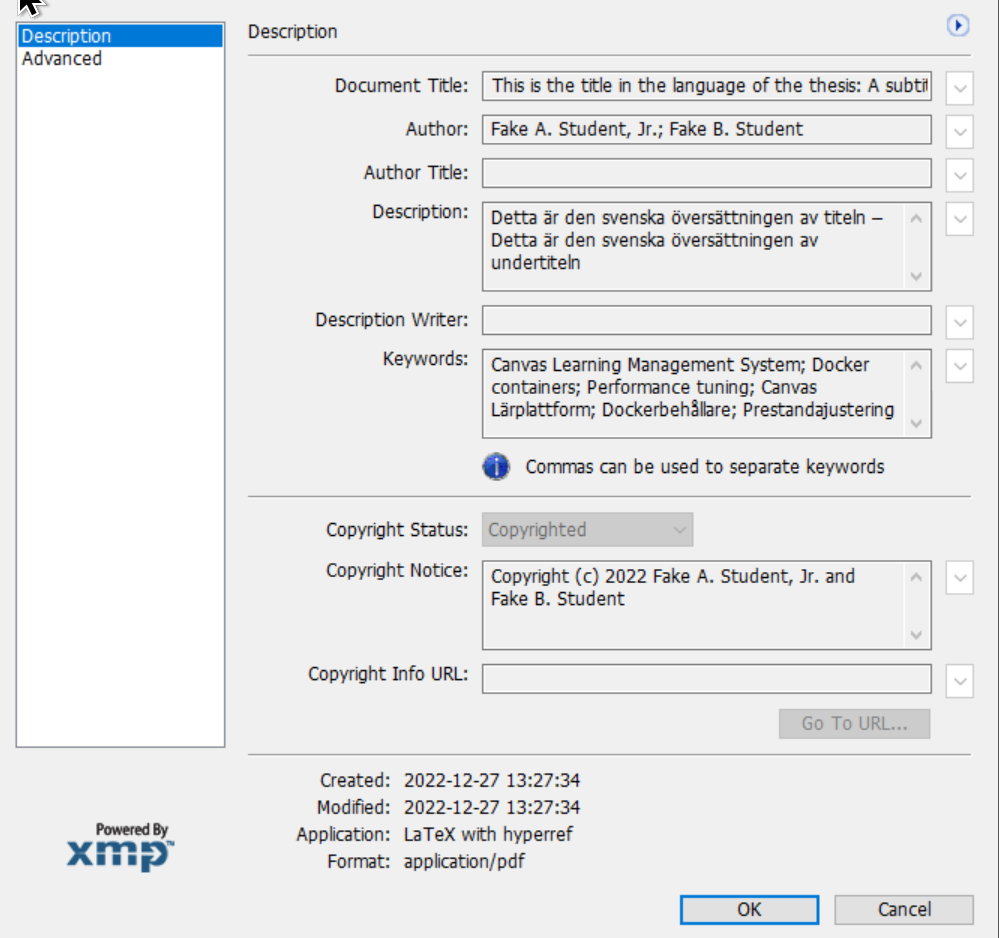
\includegraphics[width=0.99\textwidth]{README_notes/README-examiner-figures/Example-of-copyright-data-Screenshot_20221227_143035.png}
  \end{center}
  \caption{Example of the copyright information being displayed}
  \label{fig:exampleCopyrightXMPdisplayed}
\end{figure}

\Cref{lst:pdfinfoOutputPart9} shows the \texttt{dc:creator} metadata. In this case the comma separated list of authors has been rendered as an \texttt{rdf:Seq} which is an \textbf{ordered} list of items.
\begin{lstlisting}[style=myXML,
caption={The \texttt{dc:creator} metadata embedded in a PDF file}, label={lst:pdfinfoOutputPart9}]
£$\ldots$ {\color{red} continuation of the above listing}£ 
      <dc:creator>
        <rdf:Seq>
          <rdf:li>Fake A. Student, Jr.</rdf:li>
          <rdf:li>Fake B. Student</rdf:li>
        </rdf:Seq>
      </dc:creator>
\end{lstlisting}
\clearpage

\Cref{lst:pdfinfoOutputPart10} shows the \texttt{dc:subject} metadata. In this case the comma separated list of keywords has been rendered as an \texttt{rdf:Bag} which is an \textbf{unordered} list of items.
\begin{lstlisting}[style=myXML,
caption={The \texttt{dc:subject} metadata embedded in a PDF file}, label={lst:pdfinfoOutputPart10}]
£$\ldots$ {\color{red} continuation of the above listing}£ 
      <dc:subject>
        <rdf:Bag>
          <rdf:li>Canvas Learning Management System</rdf:li>
          <rdf:li>Docker containers</rdf:li>
          <rdf:li>Performance tuning</rdf:li>
          <rdf:li>Canvas Lärplattform</rdf:li>
          <rdf:li>Dockerbehållare</rdf:li>
          <rdf:li>Prestandajustering</rdf:li>
        </rdf:Bag>
      </dc:subject>
\end{lstlisting}

\Cref{lst:pdfinfoOutputPart11} shows the \texttt{dc:source} and \texttt{dc:language} metadata. The value of \texttt{dc:source} was not set explicitly, so this seems to have been derived in some way. Additionally, the \texttt{dc:language} \texttt{rdf:Bag} was automatically computed and includes all of the languages used via \textsc{babel} or \textsc{polyglossia} in the thesis.
\begin{lstlisting}[style=myXML,
caption={The \texttt{dc:source} and \texttt{dc:language} metadata embedded in a PDF file}, label={lst:pdfinfoOutputPart11}]
£$\ldots$ {\color{red} continuation of the above listing}£ 
      <dc:source>output.tex</dc:source>
      <dc:language>
        <rdf:Bag>
          <rdf:li>fr-FR</rdf:li>
          <rdf:li>es-ES</rdf:li>
          <rdf:li>nb</rdf:li>
          <rdf:li>de-DE</rdf:li>
          <rdf:li>sv</rdf:li>
          <rdf:li>it</rdf:li>
          <rdf:li>da</rdf:li>
          <rdf:li>nl</rdf:li>
          <rdf:li>et</rdf:li>
          <rdf:li>en-US</rdf:li>
        </rdf:Bag>
      </dc:language>
\end{lstlisting}

\Cref{lst:pdfinfoOutputPart12} shows the \texttt{xmp}-prefix elements in the file. This namespace is supposed to be defined at \url{http://ns.adobe.com/xap/1.0/}; however, this URL is not longer valid but the Adobe XMP Basic namespace is described at url{https://developer.adobe.com/xmp/docs/XMPNamespaces/xmp/}. In this specific case, the file provides the \texttt{CreateDate}, \texttt{xmp:ModifyDate}, \texttt{xmp:MetadataDate}, and \texttt{xmp:CreatorTool}. For the last of these the value is shown as ``LaTeX with hyperref<'' even though the \XeLaTeX~engine was used.
\begin{lstlisting}[style=myXML,
caption={The final set of metadata embedded in a PDF file}, label={lst:pdfinfoOutputPart12}]
£$\ldots$ {\color{red} continuation of the above listing}£ 
      <xmp:CreateDate>2022-12-27T10:22:34</xmp:CreateDate>
      <xmp:ModifyDate>2022-12-27T10:22:34Z</xmp:ModifyDate>
      <xmp:MetadataDate>2022-12-27T10:22:34Z</xmp:MetadataDate>
      <xmp:CreatorTool>LaTeX with hyperref</xmp:CreatorTool>
\end{lstlisting}

\Cref{lst:pdfinfoOutputPart13} shows the \texttt{xmpMM}-prefix metadata. The information about this namespace should be at \url{http://ns.adobe.com/xap/1.0/mm/}, however, this URL is no longer valid but the description of the XMP Media Management namespace is available at \url{https://developer.adobe.com/xmp/docs/XMPNamespaces/xmpMM/}.
\begin{lstlisting}[style=myXML,
caption={The \texttt{xmpMM}-prefix metadata embedded in a PDF file (two of the lines have been manually broken to fit the test in the margins)}, label={lst:pdfinfoOutputPart13}]
£$\ldots$ {\color{red} continuation of the above listing}£ 
      <xmpMM:DocumentID>uuid:d7a82bbb-620a-439b-ac90-5413339b620a£\break£</xmpMM:DocumentID>
      <xmpMM:InstanceID>uuid:620005f7-f75f-4dce-a820-a8888d18205f£\break£</xmpMM:InstanceID>
      <xmpMM:VersionID>1</xmpMM:VersionID>
      <xmpMM:RenditionClass>default</xmpMM:RenditionClass>
\end{lstlisting}

\Cref{lst:pdfinfoOutputPart14} shows the \texttt{Iptc4xmpCore}-prefix metadata. The IPTC Core Schema namespace used by the IPTC Photo Metadata standards is described briefly at \url{http://iptc.org/std/Iptc4xmpCore/1.0/xmlns/}. A full description is available at \url{https://www.iptc.org/std/Iptc4xmpCore/1.0/specification/Iptc4xmpCore_1.0-spec-XMPSchema_8.pdf}. The \texttt{Iptc4xmpCore:CreatorContactInfo} is supposed to provide enough information to enable someone reading the file to be able to contact the creator of the content. For the purposes of the thesis I have identified the authors using the KTH\_id, since one students have completed their studies at kTH their acocunts are deactivated; hence, an e-mail address is no longer meaningful.
\begin{lstlisting}[style=myXML,
caption={The \texttt{Iptc4xmpCore}-prefix metadata embedded in a PDF file}, label={lst:pdfinfoOutputPart14}]
£$\ldots$ {\color{red} continuation of the above listing}£ 
      <Iptc4xmpCore:CreatorContactInfo rdf:parseType="Resource">
        <Iptc4xmpCore:CiEmailWork>author: u100001,secondauthor: u100002</Iptc4xmpCore:CiEmailWork>
      </Iptc4xmpCore:CreatorContactInfo>
\end{lstlisting}

\Cref{lst:pdfinfoOutputPart15} shows the \texttt{prism}-prefix metadata. The Publishing Requirements for Industry Standard Metadata (PRISM) namespace should be described at \url{http://prismstandard.org/namespaces/basic/3.0/}; however, this URL is no longer valid but the PRISM Basic Metadata Specification can be found at \url{https://www.w3.org/Submission/2020/SUBM-prism-20200910/prism-basic.html}.
\begin{lstlisting}[style=myXML,
caption={The \texttt{prism}-prefix metadata embedded in a PDF file}, label={lst:pdfinfoOutputPart15}]
£$\ldots$ {\color{red} continuation of the above listing}£ 
      <prism:complianceProfile>three</prism:complianceProfile>
      <prism:subtitle xml:lang="en">A subtitle in the language of the thesis</prism:subtitle>
      <prism:aggregationType>report</prism:aggregationType>
      <prism:volume>TRITA-EECS-EX</prism:volume>
      <prism:number>2022:0000</prism:number>
      <prism:pageCount>322</prism:pageCount>
      <xmpTPg:NPages>322</xmpTPg:NPages>
\end{lstlisting}

\begin{lstlisting}[style=myXML,
caption={The final part of the metadata embedded in a PDF file}, label={lst:pdfinfoOutputPart16}]
£$\ldots$ {\color{red} continuation of the above listing}£ 
    </rdf:Description>
  </rdf:RDF>
</x:xmpmeta>
\end{lstlisting}

The \textbackslash divainfo macro was extended with the code in \Cref{lst:codeForAbstracts} to iterate through the abstracts and generate the appropriate language-tagged metadata. This macro is called at the end of the thesis to generate and output the various version of the metadata. The metadata is embedded into the PDF by means of two \LaTeX~packahes: \texttt{hyperref} and \texttt{hyperxmp}. The underlying mechanism uses the \texttt{hyperxmp} \textbackslash XMPLangAlt{lang}{pdfsubject=value} macro to store metadata by using the \texttt{lang} tags. The contents of the abstracts and languages were stored into two vectors of \texttt{scontents} buffers (lang and abstract). An \textbackslash IfEqCase macro is used to translate the three-letter ISO 639-2 Code – specifically the "B" (bibliographic) variant of these codes\footnote{note that this is the same language code used in DiVA} to the ISO 639-1 two-letter language code with an optional ISO 3166-1 two-letter region code as used by \textbackslash XMPLangAlt macro of of \texttt{hyperxmp}.
\begin{lstlisting}[style=myXML,
caption={The \textbackslash divainfo macro has been extended to output the abstracts and keywords. This code has been edited to remove the diagnostic output and to simplify it.}, label={lst:codeForAbstracts}]
%% experiment with dc:description
\newcommand{\myabstract}{abstract: unknown}
 \foreach \i in {1,...,\countsc{lang}} {
  \newcommand{\templangs}{\qgetstored{\i}{lang}}
  \tokenize{\lang}{\templangs}
   \StrSubstitute{"q"}{q}{\qgetstored{\i}{abstracts}}[\@myabstract]

    \replaceBS{\@myabstract}{\@myabstract}

    \renewcommand{\myabstract}{abstract: \@myabstract}
    %% Convert from three-letter language code to short language code
    \IfEqCase{\templangs}{
    {eng}{\XMPLangAlt{en-US}{pdfsubject={\myabstract}}}%
    {swe}{\XMPLangAlt{sv}{pdfsubject={\myabstract}}}%
    {fre}{\XMPLangAlt{fr-FR}{pdfsubject={\myabstract}}}%
    {spa}{\XMPLangAlt{es-ES}{pdfsubject={\myabstract}}}%
    {ita}{\XMPLangAlt{it}{pdfsubject={\myabstract}}}%
    {nno}{\XMPLangAlt{nn}{pdfsubject={\myabstract}}}%
    {nob}{\XMPLangAlt{nb}{pdfsubject={\myabstract}}}%
    {nor}{\XMPLangAlt{no}{pdfsubject={\myabstract}}}%
    {ger}{\XMPLangAlt{de-DE}{pdfsubject={\myabstract}}}%
    {dan}{\XMPLangAlt{da}{pdfsubject={\myabstract}}}%
    {dut}{\XMPLangAlt{nl}{pdfsubject={\myabstract}}}%
    {est}{\XMPLangAlt{et}{pdfsubject={\myabstract}}}%
    {ukr}{\XMPLangAlt{uk}{pdfsubject={\myabstract}}}%
    {lat}{\XMPLangAlt{la}{pdfsubject={\myabstract}}}%
    {fin}{\XMPLangAlt{fi}{pdfsubject={\myabstract}}}%
    {ice}{\XMPLangAlt{is}{pdfsubject={\myabstract}}}%
    {yid}{\XMPLangAlt{yi}{pdfsubject={\myabstract}}}%
    {lav}{\XMPLangAlt{lv}{pdfsubject={\myabstract}}}%
    {lit}{\XMPLangAlt{lt}{pdfsubject={\myabstract}}}%
    {pol}{\XMPLangAlt{pl}{pdfsubject={\myabstract}}}%
    {por}{\XMPLangAlt{pt}{pdfsubject={\myabstract}}}%
    {per}{\XMPLangAlt{fa}{pdfsubject={\myabstract}}}%
    {rum}{\XMPLangAlt{ro}{pdfsubject={\myabstract}}}%
    {sme}{\XMPLangAlt{se}{pdfsubject={\myabstract}}}%
    {hin}{\XMPLangAlt{hi}{pdfsubject={\myabstract}}}%
    {hun}{\XMPLangAlt{hu}{pdfsubject={\myabstract}}}%
    {bul}{\XMPLangAlt{bg}{pdfsubject={\myabstract}}}%
    {alb}{\XMPLangAlt{sq}{pdfsubject={\myabstract}}}%
    {cat}{\XMPLangAlt{ca}{pdfsubject={\myabstract}}}%
    {chi}{\XMPLangAlt{zh}{pdfsubject={\myabstract}}}%
    {ara}{\XMPLangAlt{ar}{pdfsubject={\myabstract}}}%
    {bel}{\XMPLangAlt{be}{pdfsubject={\myabstract}}}%
    {rus}{\XMPLangAlt{ru}{pdfsubject={\myabstract}}}%
    {vie}{\XMPLangAlt{vi}{pdfsubject={\myabstract}}}%
    {scc}{\XMPLangAlt{sr}{pdfsubject={\myabstract}}}% deprecated B code
    {cze}{\XMPLangAlt{cs}{pdfsubject={\myabstract}}}%
    [\typeout{unknown three-letter language code}]
    }
}
\end{lstlisting}
\clearpage
\subsection{Extending the set of languages supported for abstracts}
\label{sec:newLanguagesFOrAbstracts}
\textbf{Note for maintainers}: \Cref{lst:codeForAbstracts} will need to be extended if any additional languages are added for the abstracts. The US Library of Congress has a table of the language codes at \url{https://www.loc.gov/standards/iso639-2/php/code_list.php}.

Based upon the US Library of Congress ``Codes for the Representation of Names of Languages: Codes arranged alphabetically by alpha-3/ISO 639-2 Code'', I have eliminated all of the rows that did not have both a three-letter ISO 639-2 Code \textbf{and} a two-letter ISO 639-1 Code. For the three-letter ISO 639-2 Codes, I used only the  ``B'', \ie bibliographic codes. Based upon the above code's case statement I split the table into two parts: Languages already implemented (\Cref{tab:languagesImplemented}) and those remaining to be implemented (\Cref{tab:languagesNotImplemented}). In the course of doing this, I found that I had an incorrect entry in my case statement for ``nor'' and fixed it in the code.

According to SCB (\url{https://www.scb.se/contentassets/221c69e399f0424b852b21236952e300/sprakkoder.xlsx}) there are also ISO 639-2 codes for Yiddish with regions (see \Cref{tab:SCByiddish}). For Romanian the ISO 639-2 B code is "rum" and the ISO 639-1 code is  "ro". However, again SCB gives additional ISO 639-2 codes (see \Cref{tab:SCBromani}). For Northern Sami (Samiska, (norra)) the ISO 639-2 is "sme" and the ISO 639-1 code is "se", but is there a region code that should be used? (See \Cref{tab:SCBsami}) For Tornedalen Finnish; Meänkieli\ the ISO 639-2 code is "fit", but I am not able to determine what ISO 639-1 code should be used (see \Cref{tab:languagesMissing}). Is it "fi" with some region code? If so, what region code? 

\begin{table}[!htp]
    \caption{SCB table - Yiddish with regions}
    \label{tab:SCByiddish}
    \begin{tabular}{L{3cm}|L{6.5cm}}
      \textbf{ISO 639-2 Code} &\textbf{Swedish name of Language}\\
      \hline
YIH  &  Jiddisch (Väst)\\
YDD  &  Jiddisch (Öst)\\
\end{tabular}
\end{table}

\begin{table}[!htp]
    \caption{SCB table - Romainian with regions}
    \label{tab:SCBromani}
    \begin{tabular}{L{3cm}|L{6.5cm}}
      \textbf{ISO 639-2 Code} &\textbf{Swedish name of Language}\\
      \hline
ROM &   Romani chib\\
RMO &   Romani, Abbruzzesi, Serbisk romani, Slovensk-kroatisk romani\\
RMN &   Romani, Arli, Dzambasi, Gurbeti\\
RMC &   Romani, Bashaldo, Ungersk-slovakisk romani, Romungro\\
RMF &   Romani, Kale, Kalo\\
RMY &   Romani, Lovara, Kalderash\\
RML &   Romani, Polsk romani, Estnisk, Lettisk, Nordrysk, Vitrysk\\
RMU &   Romani, resande romani, Svensk romani, Romani tavringer\\
RMW &   Romani, Walesisk\\
\end{tabular}
\end{table}

\begin{table}[!htp]
    \caption{SCB table - Sami with regions}
    \label{tab:SCBsami}
    \begin{tabular}{L{3cm}|L{6.5cm}}
      \textbf{ISO 639-2 Code} &\textbf{Swedish name of Language}\\
      \hline
SMI &   Samiska\\
SIA &   Samiska, Akkalasamiska\\
SMN &   Samiska, Enaresamiska\\
SJK &   Samiska, Kemisamiska\\
SJD &   Samiska, Kildinsamiska\\
SMJ &   Samiska, Lulesamiska(Luleå)\\
SJE &   Samiska, Pitesamiska\\
SMS &   Samiska, Skoltsamiska\\
SMA &  Samiska, sydsamiska (södra)\\
SJT &  Samiska, Tersamiska\\
SJU &  Umesamiska\\
\end{tabular}
\end{table}
\clearpage
\begin{table}[!htp]
    \caption{Languages already implemented}
    \label{tab:languagesImplemented}
    \begin{tabular}{L{3cm}|L{3cm}|L{6.5cm}}
      \textbf{ISO 639-2 Code} & \textbf{ISO 639-1 Code} & \textbf{English name of Language}\\
      \hline
alb & sq & Albanian\\
ara & ar & Arabic\\
bel & be & Belarusian\\
bul & bg & Bulgarian\\
cat & ca & Catalan; Valencian\\
chi & zh & Chinese\\
cze & cs & Czech\\
dan & da & Danish\\
dut & nl & Dutch; Flemish\\
eng & en & English\\
est & et & Estonian\\
fin & fi & Finnish\\
fre & fr & French\\
ger & de & German\\
hin & hi & Hindi\\
hun & hu & Hungarian\\
ice & is & Icelandic\\
ita & it & Italian\\
lat & la & Latin\\
lav & lv & Latvian\\
lit & lt & Lithuanian\\
nno & nn & Norwegian Nynorsk; Nynorsk, Norwegian\\
nob & nb & Bokmål, Norwegian; Norwegian Bokmål\\
nor & no & Norwegian\\
per & fa & Persian\\
pol & pl & Polish\\
por & pt & Portuguese\\
rum & ro & Romanian; Moldavian; Moldovan\\
rus & ru & Russian\\
sme & se & Northern Sami\\
spa & es & Spanish; Castilian\\
swe & sv & Swedish\\
ukr & uk & Ukrainian\\
vie & vi & Vietnamese\\
yid & yi & Yiddish\\
\hline
   \end{tabular}
\end{table}
\FloatBarrier

\begin{table}[!ht]
    \caption{Missing languages from the Library of Congress list}
    \label{tab:languagesMissing}
    \begin{tabular}{L{3cm}|L{3cm}|L{6.5cm}}
      \textbf{ISO 639-2 Code} & \textbf{ISO 639-1 Code} & \textbf{English name of Language}\\
      \hline
fit & ??? & Tornedalen Finnish; \foreignlanguage{finnish}{Meänkieli}\\
\hline
   \end{tabular}
\end{table}
\FloatBarrier

As to the language tag to use for Meänkieli - one can simply skip the ISO 639-1 Code and use "fit" - as done in \url{https://www.msb.se/sv/om-msb/information-pa-andra-sprak/meankieli/om-msb/}.
However, it seems strange that there is not an ISO 639-1 Code. Interestingly, they use 'smi' for Lule Sami (\foreignlanguage{swedish}{lulesamiska}) on \url{https://www.msb.se/sv/om-msb/information-pa-andra-sprak/lulesamiska/om-msb/}.

\begin{longtable}{|L{3cm}|L{3cm}|L{5cm}|}
\caption{Remaining languages to implement}
\label{tab:languagesNotImplemented}\\
\hline \multicolumn{1}{|c|}{\textbf{ISO 639-2 Code}} & \multicolumn{1}{c|}{\textbf{ISO 639-1 Code}} & \multicolumn{1}{c|}{\textbf{English name of Language}} \\
\endfirsthead
\multicolumn{3}{c}%
{{\bfseries \tablename\ \thetable{} -- continued from previous page}} \\
\hline \multicolumn{1}{|c|}{\textbf{ISO 639-2 Code}} & \multicolumn{1}{c|}{\textbf{ISO 639-1 Code}} & \multicolumn{1}{c|}{\textbf{English name of Language}} \\
\hline 
\endhead
\hline \multicolumn{3}{|r|}{{Continued on next page}} \\
\hline
\endfoot
\hline
\hline
\endlastfoot
aar & aa & Afar\\
abk & ab & Abkhazian\\
afr & af & Afrikaans\\
aka & ak & Akan\\
amh & am & Amharic\\
arg & an & Aragonese\\
arm & hy & Armenian\\
asm & as & Assamese\\
ava & av & Avaric\\
ave & ae & Avestan\\
aym & ay & Aymara\\
aze & az & Azerbaijani\\
bak & ba & Bashkir\\
bam & bm & Bambara\\
baq & eu & Basque\\
ben & bn & Bengali\\
bih & bh & Bihari languages\\
bis & bi & Bislama\\
bos & bs & Bosnian\\
bre & br & Breton\\
bur & my & Burmese\\
cha & ch & Chamorro\\
che & ce & Chechen\\
chu & cu & Church Slavic; Old Slavonic; Church Slavonic; Old Bulgarian; Old Church Slavonic\\
chv & cv & Chuvash\\
cor & kw & Cornish\\
cos & co & Corsican\\
cre & cr & Cree\\
div & dv & Divehi; Dhivehi; Maldivian\\
dzo & dz & Dzongkha\\
epo & eo & Esperanto\\
ewe & ee & Ewe\\
fao & fo & Faroese\\
fij & fj & Fijian\\
fry & fy & Western Frisian\\
ful & ff & Fulah\\
geo & ka & Georgian\\
gla & gd & Gaelic; Scottish\\
gle & ga & Irish\\
glg & gl & Galician\\
glv & gv & Manx\\
gre & el & Greek, Modern (1453-)\\
grn & gn & Guarani\\
guj & gu & Gujarati\\
hat & ht & Haitian; Haitian\\
hau & ha & Hausa\\
heb & he & Hebrew\\
her & hz & Herero\\
hmo & ho & Hiri Motu\\
hrv & hr & Croatian\\
ibo & ig & Igbo\\
ido & io & Ido\\
iii & ii & Sichuan Yi; Nuosu\\
iku & iu & Inuktitut\\
ile & ie & Interlingue; Occidental\\
ina & ia & Interlingua (International Auxiliary Language Association)\\
ind & id & Indonesian\\
ipk & ik & Inupiaq\\
jav & jv & Javanese\\
jpn & ja & Japanese\\
kal & kl & Kalaallisut; Greenlandic\\
kan & kn & Kannada\\
kas & ks & Kashmiri\\
kau & kr & Kanuri\\
kaz & kk & Kazakh\\
khm & km & Central Khmer\\
kik & ki & Kikuyu; Gikuyu\\
kin & rw & Kinyarwanda\\
kir & ky & Kirghiz; Kyrgyz\\
kom & kv & Komi\\
kon & kg & Kongo\\
kor & ko & Korean\\
kua & kj & Kuanyama; Kwanyama\\
kur & ku & Kurdish\\
lao & lo & Lao\\
lim & li & Limburgan; Limburger; Limburgish\\
lin & ln & Lingala\\
ltz & lb & Luxembourgish; Letzeburgesch\\
lub & lu & Luba-Katanga\\
lug & lg & Ganda\\
mac & mk & Macedonian\\
mah & mh & Marshallese\\
mal & ml & Malayalam\\
mao & mi & Maori\\
mar & mr & Marathi\\
may & ms & Malay\\
mlg & mg & Malagasy\\
mlt & mt & Maltese\\
mon & mn & Mongolian\\
nau & na & Nauru\\
nav & nv & Navajo; Navaho\\
nbl & nr & Ndebele, South; South Ndebele\\
nde & nd & Ndebele, North; North Ndebele\\
ndo & ng & Ndonga\\
nep & ne & Nepali\\
nya & ny & Chichewa; Chewa; Nyanja\\
oci & oc & Occitan (post 1500)\\
oji & oj & Ojibwa\\
ori & or & Oriya\\
orm & om & Oromo\\
oss & os & Ossetian; Ossetic\\
pan & pa & Panjabi; Punjabi\\
pli & pi & Pali\\
pus & ps & Pushto; Pashto\\
que & qu & Quechua\\
roh & rm & Romansh\\
run & rn & Rundi\\
sag & sg & Sango\\
san & sa & Sanskrit\\
sin & si & Sinhala; Sinhalese\\
slo & sk & Slovak\\
slv & sl & Slovenian\\
smo & sm & Samoan\\
sna & sn & Shona\\
snd & sd & Sindhi\\
som & so & Somali\\
sot & st & Sotho, Southern\\
srd & sc & Sardinian\\
srp & sr & Serbian\\
ssw & ss & Swati\\
sun & su & Sundanese\\
swa & sw & Swahili\\
tah & ty & Tahitian\\
tam & ta & Tamil\\
tat & tt & Tatar\\
tel & te & Telugu\\
tgk & tg & Tajik\\
tgl & tl & Tagalog\\
tha & th & Thai\\
tib & bo & Tibetan\\
tir & ti & Tigrinya\\
ton & to & Tonga (Tonga Islands)\\
tsn & tn & Tswana\\
tso & ts & Tsonga\\
tuk & tk & Turkmen\\
tur & tr & Turkish\\
twi & tw & Twi\\
uig & ug & Uighur; Uyghur\\
urd & ur & Urdu\\
uzb & uz & Uzbek\\
ven & ve & Venda\\
vol & vo & Volapük\\
wel & cy & Welsh\\
wln & wa & Walloon\\
wol & wo & Wolof\\
xho & xh & Xhosa\\
yor & yo & Yoruba\\
zha & za & Zhuang; Chuang\\
zul & zu & Zulu\\
\end{longtable}
\FloatBarrier
%\end{document}

\subsection{Extending the set of elements for theses}
\label{sec:newMetadataForTheses}
Even with all of the various schema included in XMP, there is a lot of metadata that is needed for DiVA that can not yet easily be included and embedded in XMP. Thus, for the present, the extra metadata needs to be collected and processed via some mechanism other than XMP.

For XMP, there are some specific areas that might be of interest in the future:
\begin{itemize}
  \item Adding new dc elements (§\,\ref{sec:newDCelements}) 
  \item Adding references to the metadata (§\,\ref{sec:addingReferences}), and 
  \item Adding citation data to the metadata (§\,\ref{sec:addingCitation})
\end{itemize}

\subsubsection{Adding new dc elements}
\label{sec:newDCelements}
In \Cref{tab:dublicCoreDigitalCommons} on \pageref{tab:dublicCoreDigitalCommons} we saw five elements that are perhaps worth adding, specifically:
\texttt{thesis.degree}, \texttt{thesis.degree.discipline}, \linebreak[4]\texttt{thesis.degree.grantor}, \texttt{thesis.degree.level}, and \linebreak[4] \texttt{thesis.degree.name}. It is potentially worth adding these in the future to the XMP data for a thesis. For some discussion of these elements, please see the discussion of EDT‐MS metadata elements in the paper by Ivanović, Ivanović, and Surla entitled ``A data model of theses and dissertations compatible with {CERIF}, {Dublin} {Core} and {EDT}‐{MS}''\cite{ivanovic_data_2012}. ETD-MS is defined in ``ETD-MS v1.1: an Interoperability Metadata Standard for Electronic Theses and Dissertations''\,\cite{hickey_pavani_suleman_2010} and available at \url{https://ndltd.org/wp-content/uploads/2021/04/etd-ms-v1.1.html}.


\subsubsection{Adding references to the metadata}
\label{sec:addingReferences}
Increasingly, there is an interest in being able to easily know what references have been cited by a thesis. Part of this interest is to be able to compute citation maps (who cites whom) and to examine the types of sources that are cited.

There are several possibilities for storing information about references. One is the element \texttt{dc.relation.references}. Another possibility is to use the \texttt{dcterms:references} element refinement of \texttt{dc:relation} as proposed in 1998 by Ann Apps of the DCMI Citations Working Group (\url{https://www.dublincore.org/groups/citation/}).

More recently, there is a new schema proposed by CrossRef, see \url{https://www.crossref.org/documentation/schema-library/markup-guide-metadata-segments/references/}. Note that the focus of this work is to facilitate depositing with CrossRef the list of references used in a publication. Their set of elements is shown in \Cref{tab:crossRefElementsForCitationTagging}\footnote{\url{https://www.crossref.org/documentation/schema-library/markup-guide-metadata-segments/references/\#00178}}. Note that while the focus seems to be on journal articles, they also have a ``Metadata best practices'' website with lots of examples of metadata for different types of documents, see \url{https://www.crossref.org/documentation/principles-practices/best-practices/}.

\begin{table}[!ht]
    \caption{CrossRef elements for citation tagging}
    \label{tab:crossRefElementsForCitationTagging}
    \begin{tabular}{l}
      \textbf{Element}\\
      \hline
issn\\
journal\_title\\
author\\
volume\\
issue\\
first\_page\\
cYear\\
article\_title\\
isbn\\
series\_title\\
volume\_title\\
edition\_number\\
article\_title\\
std\_designator\\
standards\_body\_name\\
standards\_body\_acronym\\
component\_number\\
unstructured\_citation\\
doi\\
\end{tabular}
\end{table}

\subsubsection{Adding citation data to the metadata}
\label{sec:addingCitation}
There is also a desire by many to include bibliographic citation information into the XMP so that the PDF carries this data and one does \emph{not} need to access some other source to find this information. The element \texttt{DCTERMS.bibliographicCitation} is proposed for this purpose in a document by Ann Apps, ``Guidelines for Encoding Bibliographic Citation Information in Dublin Core™ Metadata''\,\cite{Ann_Apps_2005}.

Note that to include the URN and DiVA identifiers assigned by DiVA, you first need to create a DiVA entry and then use the assigned values to update the XMP information in the PDF file \textit{before} uploading the fill text to DiVA.

\section{Future work: Better exploiting unicode}
\label{sec:betterExploitingUnicode}

The current design of storing the \LaTeX\ commands in an \textsc{scontents} buffer and then retrieving them \textit{without} expanding the \LaTeX\ macros makes it possible to post-process these commands and make content that is suited for making announcements of the oral presentation, making calendar entries for this presentation, and generating the abstracts for the MODS file for DiVA. However,  if one wants to take the full leap to unicode, this is perhaps not a good design choice - as it requires that all of the processing that \LaTeX\ could do of the unicode is not done and that the programs that extract the unexpanded contents will have to keep changing to keep up with want \LaTeX\ macros are used. 

There might seem to be two alternatives:
\begin{enumerate}
    \item Keep modifying the extraction programs as needed or
    \item Only allow the use of \LaTeX\ macros that expand into unicode; thus, not allowing environments and commands such as \textbackslash textbf\{\}, \textbackslash textif\{\}, etc. that do not translate into characters that can be written in unicode.
\end{enumerate}

In the second alternative, one might think about translating the string inside a \textbackslash textbf\{\} into unicode characters in the Bold, Latin, uppercase \& lowercase range, \ie U+1D400 to U+1D433 (there is a similar transformation possible for Greek). The characters are defined in the \textsc{unicode-math} package. Logically, this would be similar to redefining \textbackslash textbf\{\} as \textbackslash mathtextbf\{\}\footnote{\textbackslash mathtextbf\{\} cannot be used directly as it only works in math mode.}.  

For \textbackslash textif\{\} one could utilize the Italic, Latin, uppercase  and lowercase range, \ie U+1D434 to U+1D467 (there is a similar transformation possible for Greek). Similar transformations are possible for \textbackslash texttt\{\}
using Typewriter, Latin, uppercase \& lowercase and for \textbackslash textsc\{\}

Additionally, there is a  Bold italic, Latin, uppercase \& lowercase range, \ie U+1D468 to U+1D49B.

However, the above two alternatives are not actually alternatives -- as the \textsc{scontents} buffers are output in a \textsc{verbatimsc} environment - hence they do not get expanded at all and therefore all of the use of \textsc{scontents} buffers to provide values for \textsc{hyperxmp} will not be expanded. One possibility might be to use the expanded output of the buffers in the DiVA metadata for abstracts.

%\end{document}

%\fi
%\end{comment}

%\begin{comment}
%% Information for administrators
%\ifxeorlua
%\cleardoublepage
%%\documentclass[../examplethesis.tex]{subfiles}
%\begin{document}
\chapter{DiVA administrator viewpoint}
\label{ch:adminViewpoint}

This chapter, written by Gerald Q. Maguire Jr.,  describes the implications of the thesis templates I have developed for use at KTH from the viewpoint of a DiVA administrator. Other documents provide the template which also contains information for authors and information about why the template is the way that it is. This document provides some information for DiVA administrators about the template and how it can be used with some programs to help make the degree process easier for students, faculty, and administrators while at the same time \textbf{greatly} reducing the work needed to report a thesis into DiVA.

An assumption for readers of this document is that you know KTH-speak, including the various acronyms that are used.

\textbf{This document is a work in progress.}

\section[Introduction to templates for DiVA administrators]{Introduction to templates for\\ DiVA administrators}

The assumption is that a student has written their thesis starting with either a DOCX document or \LaTeX\~project that have used the thesis templates; these are marked as ``DOCX using template'' and ``\LaTeX project using template'' (respectively), see \Cref{fig:forDiVAAdmins}. The key idea is to have these sources include  \first the information that is need for input into DiVA and \Second the information that can be used to produce and apply a cover to the resulting PDF file that will be uploaded into DiVA (either just for archiving or for also making the full-text available).

The ``DOCX using template'' and ``\LaTeX project using template'' are input to their respective programs as usual by the student to produce a PDF file (marked as ``PDF using template'') and possibly other files. This PDF file has one or more pages at the end of it that are in a section with a heading of ``For DIVA'' or this same string with four euro symbols (\ie `€') before and after the string with a space before and after the string. An example of the top of such a page is shown in \Cref{fig:topOfForDiva}.  At a minimum all of the data is now collected in one spot from which in the worst case one can cut-and-paste it into a single JSON file; however, some programs have been developed to mechanically extract this data, as will be described in \Cref{sec:gettingNecessaryData} - thus avoiding the need to cut-and-paste $\Rightarrow$ more fika time.

\tikzset{
    processBox/.style={rectangle, rounded corners, minimum width=3cm, minimum height=1cm,text centered, draw=black, fill=red!20},
    destinationBox/.style={rectangle, rounded corners, minimum width=3cm, minimum height=1cm,text centered, draw=black, fill=green!10},
    arrow/.style={thick,->,>=stealth}
}

\begin{figure}[!ht]
\resizebox{1.1\textwidth}{!}{%
\begin{tikzpicture}
[align=left,node distance=2cm]



\node (DOCXFile) [tape,tape bend top=none,draw,font=\sffamily] {DOCX using template};
\node (latexFile) [tape,tape bend top=none,draw,font=\sffamily, right=0.5cm of DOCXFile] {\LaTeX project using template};




\node (LaTeX) [processBox,  below=5cm of latexFile] {LaTeX compiler};
\node (latexjsonFile) [tape,tape bend top=none,draw,font=\sffamily, below of=LaTeX] {fordiva.json};



\node (extractDOCX) [processBox, below=8cm of DOCXFile] {extract\_custom\_DOCX\_properties};
\node (PDFfile) [tape,tape bend top=none,draw,font=\sffamily, left=5cm of LaTeX] {PDF using template};
\node (Word) [processBox,  above=3cm of PDFfile] {Word or similar};
\node (extractor) [processBox, below=6cm of PDFfile] {extract\_pseudo\_JSON-from\_PDF};

\node (cleanJSONfromLaTeX) [processBox, below=4cm of LaTeX] {cleanup\_pseudo\_JSON-from\_LaTeX};
\node (jsonFile) [tape,tape bend top=none,draw,font=\sffamily, below=4cm of cleanJSONfromLaTeX] {JSON file};

\node (assignTRITA) [processBox, below=3cm of jsonFile] {Assign TRITA number};
\node (jsonFileWithTRITA) [tape,tape bend top=none,draw,font=\sffamily, below of=assignTRITA] {JSON file with TRITA};
\node (jsontoMODS) [processBox, below of=jsonFileWithTRITA] {JSON\_to\_MODS};

\node (acronymsfile) [tape,tape bend top=none,draw,font=\sffamily, right=4.5cm of cleanJSONfromLaTeX] {acronyms.tex};

\node (TRITAlist) [destinationBox, right=1cm of assignTRITA] {TRITA list/database};

\node (modsFileWithTRITA) [tape,tape bend top=none,draw,font=\sffamily, below of=jsontoMODS] {MODS file with TRITA};
\node (makeApplyCover) [processBox, below of=modsFileWithTRITA] {Make and apply cover};
\node (divameta) [destinationBox, right=1cm of modsFileWithTRITA] {Import MODS file into DiVA};
\node (diva) [destinationBox, right=1cm of makeApplyCover] {Upload PDF into DiVA};


\draw [red, dashed]   (PDFfile) to[out=-120,in=180] (makeApplyCover);
\draw [red, dashed]   (Word) to[out=-90,in=90] (PDFfile);
\draw [red, dashed]   (LaTeX) to[out=-180,in=90] (PDFfile);
\draw [arrow] (DOCXFile) --  (extractDOCX.north);
\draw [arrow] (extractDOCX) --  (jsonFile.north west);
\draw [arrow] (latexFile.south) --  (LaTeX.north);
\draw [arrow] (LaTeX) --  (latexjsonFile.north);
\draw [arrow] (latexjsonFile) --  (cleanJSONfromLaTeX.north);
\draw [arrow] (cleanJSONfromLaTeX.south) --  (jsonFile.north);
\draw [red, dashed] (PDFfile) --  (extractor.north);
\draw [arrow] (DOCXFile) --  (Word.north);
\draw [arrow] (extractor.south) --  (jsonFile.west);
\draw [arrow] (jsonFile) --  (assignTRITA);
\draw [arrow] (jsontoMODS) --  (modsFileWithTRITA);
\draw [arrow] (modsFileWithTRITA) --  (divameta);
\draw [arrow] (assignTRITA) --  (jsonFileWithTRITA);
\draw [arrow] (jsonFileWithTRITA) --  (jsontoMODS);
\draw [arrow] (modsFileWithTRITA) --  (makeApplyCover);
\draw [arrow] (makeApplyCover) --  (diva);
\draw [arrow] (latexFile.south east) --  (acronymsfile.north);
\draw [arrow] (acronymsfile.south east) to[out=-45,in=0]  (jsontoMODS.east);
\draw [arrow] (TRITAlist) --  (assignTRITA.east);
\draw [arrow] (assignTRITA) --  (TRITAlist.west);

\end{tikzpicture}
}
\caption{Figure shows the flow of data relevant to DiVA administrators - the dashed red line shows the PDF, while the black lines show other types of data}
  \label{fig:forDiVAAdmins}
\end{figure}

\begin{figure}[!ht]
  \begin{center}
    
\includegraphics[width=0.99\textwidth]{README_notes/README-examiner-figures/for_diva_top_lines_Screenshot_20220403_164821.png}
  \end{center}
  \caption{Top of the page of data for DiVA}
  \label{fig:topOfForDiva}
\end{figure}
\FloatBarrier

\section{Getting the necessary data}
\label{sec:gettingNecessaryData}
The collected data shown in \Cref{fig:topOfForDiva} is roughly in a format called JavaScript Object Notation (JSON) and described in \Cref{sec:json}. There are several cases to consider for how to extract this information; then, given the information in JSON it is possible to generate a MODS file that can be imported into DiVA:
\begin{itemize}
    \item  \LaTeX~project - as described in \Cref{sec:extractingJSONLaTeX},
    \item DOCX file - as described in \Cref{sec:extractingJSONDOCX}, or
    \item PDF using template - as described in \Cref{sec:extractingJSONPDF}.
\end{itemize}


\subsection {JSON}
\label{sec:json}
JSON is a standard way of representing structured data as text. An example of this text is shown in \Cref{lst:forDIVAtop}. This format is useful as it is \first readily readable by both humans and computers and \Second is easy to edit, and \third is commonly supported by many programming languages. The basic element is of the form: \textquotedbl label\textquotedbl: value\ where label is a string and value can be another string or a structure (an element inside curly braces). String values are within double quote marks. A label of \textquotedbl First name\textquotedbl and the value \textquotedbl Fake A.\textquotedbl~is shown in line \ref{line:firstName} of the listing below. This is part of a structure that gives a value for \textquotedbl Author1\textquotedbl~and this value is a structure with a list of elements for \textquotedbl Last name\textquotedbl, \textquotedbl First name\textquotedbl, \textquotedbl Local User Id\textquotedbl~(\ie the kthid), \textquotedbl E-mail\textquotedbl, and \textquotedbl organisation \textquotedbl. The organisation in turn can have multiple levels where the first level L1 is the school, L2 is a department, and L3 is a division. In a discussion with DiVA administrators at KTH on 2021-04-29, the consensus was that the organizational affiliation of students should be the school of the thesis examiner, since 1\textsuperscript{st} and 2\textsuperscript{nd} cycle students are in \textbf{programs of study} and not schools, department, \etc.

\begin{lstlisting}[language=json, numbers=left,
    stepnumber=1, escapechar=|, caption={Text version of the top of the For DIVA output (reformatted to bring out the structure and improve readability - line numbers are added just in the listing)}, label=lst:forDIVAtop]
{
"Author1": { 
    "Last name": "Student",
    "First name": "Fake A.", |\label{line:firstName}|
    "Local User Id": "u100001",
    "E-mail": "a@kth.se",
    "organisation": {"L1": "School of Electrical Engineering and Computer Science",}
},
"Author2": {
    "Last name": "Student",
    "First name": "Fake B.",
    "Local User Id": "u100002",
    "E-mail": "b@kth.se",
    "organisation": {"L1": "School of Architecture and the Built Environment",}
},
"Cycle": "1",
"Course code": "IA150X",
"Credits": "15.0",
"Degree1": {
    "Educational program": "Bachelor's Programme in Information and Communication Technology",
    "Programcode": "TCOMK",
    "Degree": "Bachelors degree", |\label{line:degree}|
    "subjectArea": "Technology"   |\label{line:subjectarea}|
},
"Title": {
    "Main title": "This is the title in the language of the thesis",
    "Subtitle": "A subtitle in the language of the thesis",
    "Language": "eng" },
"Alternative title": {
    "Main title": "Detta är den svenska översättningen av titeln",
    "Subtitle": "Detta är den svenska översättningen av undertiteln",
    "Language": "swe"
},
\end{lstlisting}

\subsection{Case of \LaTeX~project}
\label{sec:extractingJSONLaTeX}

In the case of an \LaTeX~project, when compiling the \LaTeX~as a side-effect a \texttt{fordiva.json} file is generated, if you save this file locally then you can clean it up and make a MODS file with the following commands:
\Needspace*{4\baselineskip}
\begin{lstlisting}[basicstyle=\footnotesize, language={bash}, caption={Cleanup pseudo JSON produced by the \LaTeX~compiler and then make a MODS file},label=lst:AdmincleanPseudoJSONandConvertToMODS]
./cleanup_pseudo_JSON-from_LaTeX.py --json fordiva.json --acronyms acronyms.tex
./JSON_to_MODS.py --json fordiva-cleaned.json
\end{lstlisting}

Now all you have to do is rename the XML file (\texttt{modsXML.xml}) that was produced to \texttt{xxx.mods} and you are all set to upload the MODS file into DiVA!

To find the \texttt{fordiva.json} file in the \LaTeX project in Overleaf, look for the “Other logs and files” button shown at the bottom of the log output window. After clicking this button you will see a list of log and other files and can now download it.

Note that if the student has used the glossaries package to use acronyms in the abstract(s) they also need to provide an \texttt{acronyms.tex} file.

\generalExpl{Should the student submit the \texttt{fordiva.json} and \texttt{acronyms.tex} file via Canvas (along with their PDF file)?}

\subsection{Case of DOCX file}
\label{sec:extractingJSONDOCX}
In the case of a DOCX file using the template\footnote{The DOCX template (\eg Template-thesis-English-2022-with-for-DiVA.docx is available from available from \url{https://github.com/gqmaguirejr/E-learning} ) while information about using the DOCX template is in the document ``Proposal for a standard thesis template: DOCX version(s)'' available from the same GitHub.}, the JSON data can be extracted directly from the DOCX file and a MODS file created as shown in \Cref{lst:extractDOCX}.
\Needspace*{4\baselineskip}
\begin{lstlisting}[basicstyle=\footnotesize, language={bash}, caption={Extract field values from the DOCX file and then make a MODS file},label=lst:extractDOCX]
./extract_customDocProperties.py filename.docx --json output.json
./JSON_to_MODS.py --json output.json
\end{lstlisting}
If the –-json option is not included in the arguments to\linebreak[4] \texttt{extract\_customDocProperties.py}, the output file is by default “output.json”.

Note that the program can be given an argument of either \texttt{\hbox{–-English}} or \texttt{\hbox{–-Swedish}} to explicitly set the language for the body text. Otherwise, the choice is made based upon the default language (w:lang) specified in the word/settings.xml file.

\warningExpl{Perhaps a custom property for the language of the document should be added.}

The number of pages of the preface and body of the document is taken from the result of the page references to the two bookmarks as generated in the “For DIVA” data. One cannot derive this data directly but only by extracting the data from the word/document.xml file (\textit{after} the word processing package has generated the textual representation for these markers – since their values depends upon the layout and pagination of the document).

A major limitation is that this program only supports extracting English and Swedish abstracts (and keywords); hence abstracts in other languages are \textbf{not} extracted. Additionally, the support for HTML markup in the abstracts is limited to paragraphs. 


\generalExpl{Should the student submit the \texttt{output.json} file via Canvas (along with their PDF file)?}

\subsection{Case of PDF using template file}
\label{sec:extractingJSONPDF}
If all you have is a ``PDF using template file'' then one can extract the information using the program \texttt{extract\_pseudo\_JSON-from\_PDF.py}.  Given a ``PDF using template'' file (and if a \LaTeX~project has been used the acronyms.tex file):
\begin{enumerate}
    \item Save the PDF file of the thesis, for example: \texttt{oscar.pdf}
    \item Extract the “For DIVA” information as JSON, as shown in \Cref{lst:AdminextractPseudoJSONFromPDFforOscarFileToJSON}
    
    If acronyms are used in the abstracts, you can add the “--acronyms acronyms.tex” argument to the extract command line and the program will process the acronyms from the acronyms.tex file (this means that you will also need this file). The output of the program is a JSON file (oscar.json) that can subsequently be used to make an announcement.
\end{enumerate}
\Needspace*{7\baselineskip}
\begin{lstlisting}[basicstyle=\footnotesize, language={bash}, caption={Commands to extract pseudo JSON from the PDF file for Oscar}, label=lst:AdminextractPseudoJSONFromPDFforOscarFileToJSON]    
./extract_pseudo_JSON-from\_PDF.py --pdf oscar.pdf --json oscar.json
./JSON_to_MODS.py --json oscar.json
\end{lstlisting}

\generalExpl{Should the student submit the \texttt{xxxx.json} file and possibly the acronyms.text file via Canvas (along with their PDF file)?}

\subsection{TRITA}
Unless the Office of Student Affairs is going to assign TRITA numbers before the thesis has a cover made, then I think that the Office of Student Affairs has to assign the TRITA number and then \textbf{make and apply the cover}. The current method of making and applying covers before the PDF is submitted to the Office of Student Affairs is foolish and unnecessary. It is easy to specify the TRITA string as an argument when making the MODS file, as shown in \Cref{lst:specifyTRITA}. 
\begin{lstlisting}[basicstyle=\footnotesize, language={bash}, caption={Command to make a MODS file with a specified TRITA string}, label=lst:specifyTRITA]
./JSON_to_MODS.py --json fordiva.json --trita "TRITA-XXX-EX-2021:219"
\end{lstlisting}

This requires that the student provide the information about the degree that they will apply for and the subject area \textbf{within} their document so that it ends up in the JSON file. This was done in lines  \ref{line:degree} and \ref{line:subjectarea} in \Cref{lst:forDIVAtop}.

\subsection{Covers}
A DOCX cover can be made for a thesis using the \texttt{JSON\_to\_DOCX\_cover.py} command shown in \Cref{lst:JSONtoDOCXcover}. This command supports the many different types of exams. It also can take many optional parameters that will over ride the contents of the JSON file (by default the JSON file name is assumed to be \texttt{calendar\_event.json}) as shown in \Cref{lst:JSONtoDOCXcover2}. If the \texttt{\hbox{-\,-language sv}} command is used or the language of the main title is Swedish (indicate in the JSON file as `swe'') the program eliminates the English KTH logotype and changes the course name appropriately. The field of technology or main subject have to be in the selected language, shown in \Cref{lst:JSONtoDOCXcover2}. Note that you can optionally specify the TRITA string on the command line with an option of the form:
\texttt{\hbox{-\,-TRITA  "TRITA-XXX-EX-2022:99999"}}.

\begin{lstlisting}[escapechar=|, basicstyle=\footnotesize, language={bash}, caption={Command to make a cover DOCX file with a specified TRITA string}, label=lst:JSONtoDOCXcover]
./JSON_to_DOCX_cover.py --file  Omslag_Exjobb_Eng_en-20220325.docx |\textbackslash \\| --exam kandidatexamen  --trita "TRITA-XXX-EX-2021:0000"
\end{lstlisting}

\begin{lstlisting}[escapechar=|, basicstyle=\footnotesize, language={bash}, caption={Command to make a cover DOCX file with the specified values}, label=lst:JSONtoDOCXcover2]
./JSON_to_DOCX_cover.py --file Omslag_Exjobb_Eng_en-20220325.docx|\textbackslash \\| --cycle 2 --credits 30.0 --area "bioteknik" --area2 "kemiteknik"|\textbackslash \\| --exam both --trita "TRITA-CBH-EX-2021:00"|\textbackslash \\| --language sv  --json calendar-sv.json
\end{lstlisting}

\textbf{NB}: The program is explicitly designed to work with the English version of the template from 2022-03-25, hence the specification of the template used in the two examples above.

\warningExpl{TODO: Make a program to make and apply the correct cover to the PDF file. Otherwise, one can use the specific templates shown at \url{https://canvas.kth.se/courses/11/pages/templates-for-1st-and-2nd-cycle-theses-some-templates}.}

\textbf{NB}: The current \LaTeX~template makes the front and back covers and uses a TRITA string specified in the \LaTeX~project files. The command shown in \Cref{lst:specifyTRITA} overrides this value when making the MODS file, but the existing TRITA string on the back cover has to be manually edited.

\warningExpl{Perhaps a solution is to integrate the \textbf{front} cover into both the \LaTeX and the DOCX templates and have the Office of Student Affairs apply only the back cover - as this is where the TRITA number appears.}

\textbf{NB}: The ``For DIVA'' pages need to be removed from the PDF file before uploading the PDF file into DiVA.

\section[Inserting information into LADOK]{Inserting information into LADOK}
\label{sec:JSONtoLADOKDiVAAdmis}
As part of the effort to be able to minimize the effort of cutting and pasting. I have made a program JSON\_to\_ladok.py that takes the extracted JSON information and uses the information about the author(s) and the title and alternative title to try to insert this information into LADOK for the module (\ie ``moment'' in Swedish) that requires a project title, \ie, 'KravPaProjekttitel' is True. \Cref{lst:usingExtractedJSONtoProduceLADOKentry1} shows an example of using this program to try to put the title and alternative title into LADOK. Basically the program logic should work, but I do \textbf{not} have the required permission to make entries of this sort of data for a degree project (\ie Rapporteringsrättighet saknas).

Note that this program uses the \texttt{ladok3} python library but extends it with some features that are not (yet) in the library. \textbf{It should be regarded as very much a work in progress.} However, it illustrates what could be done using the information in the JSON file.
\begin{lstlisting}[language={bash},
    breaklines=true,
    breakatwhitespace=true,          % sets if automatic breaks should only happen at whitespace
    breakindent=0em,
    caption={Using the extracted JSON to produce a LADOK entry for a student in the DA231X degree project course}, label=lst:usingExtractedJSONtoProduceLADOKentry1]
./JSON_to_ladok.py --json xxx.json 
...
author={'Last name': 'xxx', 'First name': 'yyy', 'Local User Id': 'u1xxxx', 'E-mail': 'oxxx@kth.se', 'organisation': {'L1': 'School of Electrical Engineering and Computer Science '}}
Canvas user_id=dddd
integration_id=gggggg-gggg-gggg-gggg-ggggggg
ladoK_course_info={'id': '6683207e-5a5d-11eb-9b32-eeb44fb14647', 'round_id': '8e15ae14-1d86-11ea-a622-3565135944de', 'education_id': '374ea085-73d8-11e8-afa7-8e408e694e54', 'instance_id': '8eee8da9-dd0a-11e8-bb7a-19f8cd1a470e', 'swe_name': 'Examensarbete i datalogi och datateknik, avancerad nivå', 'eng_name': 'Degree Project in Computer Science and Engineering, Second Cycle'}
moment code=PRO1, requires title=False
moment code=PRO2, requires title=False
moment code=PRO3, requires title=True
trying to store a passing grade for moment=PRO3
Traceback (most recent call last):
  File "./JSON_to_ladok.py", line 533, in <module>
    sys.exit(main(sys.argv[1:]))
  File "./JSON_to_ ladok.py", line 519, in main
    status=save_result_degree_project3(ladok, integration_id, course_code, mom['Utbildningskod'], '2021-07-14', 'P', "PF", main_title, alternative_main_title)
  File "./JSON_to_ ladok.py", line 374, in save_result_degree_project3
    raise Exception("Couldn't register " + course_moment + "=" + grade_raw + " " + result_date_raw + ": " + r.json()["Meddelande"])
Exception: Couldn't register PRO3=P 2021-07-14: Hinder mot skapa resultat påträffat: Rapporteringsrättighet saknas
\end{lstlisting}

\warningExpl{There is currently a transfer to LADOK project within the group of developers at the IT unit who are working on E-learning - they have been working on an API for entering the title(s) and other information (just as they are making it possible to use a program to enter grades and dates for other courses).}


\section{The examiners can also use the JSON file}

\Cref{fig:overallDataflow} shows the overall data flow starting with either a DOCX document or \LaTeX\~project that has used the thesis templates. Not only is the JSON data useful with respect to DiVA, but it can also be used for other purposes. For example, as shown in \Cref{fig:overallDataflow}, an examiner can use it for announcing the student's oral presentation via the Canvas course room and calendar and potentially in the KTH Cortina Calendar.

However, as calendar entries were not relevant to DiVA administrators, this figure was simplified in \Cref{fig:forDiVAAdmins}.

\begin{figure}[!ht]
\resizebox{1\textwidth}{!}{%
\begin{tikzpicture}
[align=left,node distance=2cm]



\node (DOCXFile) [tape,tape bend top=none,draw,font=\sffamily] {DOCX using template};
\node (latexFile) [tape,tape bend top=none,draw,font=\sffamily, right=0.5cm of DOCXFile] {\LaTeX project using template};




\node (LaTeX) [processBox,  below=5cm of latexFile] {LaTeX compiler};
%\node (acronymsfile) [tape,tape bend top=none,draw,font=\sffamily, right=2cm of latexFile] {acronyms.tex};
\node (latexjsonFile) [tape,tape bend top=none,draw,font=\sffamily, below of=LaTeX] {fordiva.json};



\node (extractDOCX) [processBox, below=8cm of DOCXFile] {extract\_custom\_DOCX\_properties};
\node (PDFfile) [tape,tape bend top=none,draw,font=\sffamily, left=5cm of LaTeX] {PDF using template};
\node (Word) [processBox,  above=3cm of PDFfile] {Word or similar};
\node (extractor) [processBox, below=6cm of PDFfile] {extract\_pseudo\_JSON-from\_PDF};

\node (cleanJSONfromLaTeX) [processBox, below=4cm of LaTeX] {cleanup\_pseudo\_JSON-from\_LaTeX};
\node (jsonFile) [tape,tape bend top=none,draw,font=\sffamily, below=4cm of cleanJSONfromLaTeX] {JSON file};

\node (start) [processBox, right=0.5cm of jsonFile] {JSON\_to\_calendar};

\node (assignTRITA) [processBox, below=3cm of jsonFile] {Assign TRITA number};
\node (jsonFileWithTRITA) [tape,tape bend top=none,draw,font=\sffamily, below of=assignTRITA] {JSON file with TRITA};
\node (jsontoMODS) [processBox, below of=jsonFileWithTRITA] {JSON\_to\_MODS};
%\node (modsFile) [tape,tape bend top=none,draw,font=\sffamily, below of=jsontoMODS] {MODS file};

\node (calendarEvent) [destinationBox, right=1cm of start] {Canvas calendar event};
\node (announcement) [destinationBox,  above of =calendarEvent] {Canvas announcement};
\node (acronymsfile) [tape,tape bend top=none,draw,font=\sffamily, right=4.5cm of cleanJSONfromLaTeX] {acronyms.tex};
\node (cortinaCalendarEvent) [destinationBox,  right=0.5cm of start, below of=calendarEvent] {KTH Cortina calendar event};
\node (TRITAlist) [destinationBox, right=1cm of assignTRITA] {TRITA list/database};

\node (modsFileWithTRITA) [tape,tape bend top=none,draw,font=\sffamily, below of=jsontoMODS] {MODS file with TRITA};
\node (makeApplyCover) [processBox, below of=modsFileWithTRITA] {Make and apply cover};
\node (divameta) [destinationBox, right=1cm of modsFileWithTRITA] {Import MODS file into DiVA};
\node (diva) [destinationBox, right=1cm of makeApplyCover] {Upload PDF into DiVA};


\draw [red, dashed]   (PDFfile) to[out=-120,in=180] (makeApplyCover);
\draw [red, dashed]   (Word) to[out=-90,in=90] (PDFfile);
\draw [red, dashed]   (LaTeX) to[out=-180,in=90] (PDFfile);
\draw [arrow] (DOCXFile) --  (extractDOCX.north);
\draw [arrow] (extractDOCX) --  (jsonFile.north west);
\draw [arrow] (latexFile.south) --  (LaTeX.north);
\draw [arrow] (LaTeX) --  (latexjsonFile.north);
\draw [arrow] (latexjsonFile) --  (cleanJSONfromLaTeX.north);
\draw [arrow] (cleanJSONfromLaTeX.south) --  (jsonFile.north);
\draw [red, dashed] (PDFfile) --  (extractor.north);
\draw [arrow] (DOCXFile) --  (Word.north);
\draw [arrow] (extractor.south) --  (jsonFile.west);
\draw [arrow] (jsonFile) --  (assignTRITA);
\draw [arrow] (jsonFile) --  (start.west);
\draw [arrow] (start.east) --  (announcement.west);
\draw [arrow] (start.east) -- (calendarEvent);
\draw [arrow] (start.east) -- (cortinaCalendarEvent.west);
%\draw [arrow] (jsonFile) --  (jsontoMODS.north west);
%\draw [arrow] (jsontoMODS) --  (modsFile);
%\draw [arrow] (jsontoMODS) --  (modsFile);
\draw [arrow] (jsontoMODS) --  (modsFileWithTRITA);
%\draw [arrow] (modsFile) --  (assignTRITA);
\draw [arrow] (modsFileWithTRITA) --  (divameta);
\draw [arrow] (assignTRITA) --  (jsonFileWithTRITA);
\draw [arrow] (jsonFileWithTRITA) --  (jsontoMODS);
\draw [arrow] (modsFileWithTRITA) --  (makeApplyCover);
\draw [arrow] (makeApplyCover) --  (diva);
%\draw [arrow] (assignTRITA) --  (modsFileWithTRITA);
\draw [arrow] (latexFile.south east) --  (acronymsfile.north);
\draw [arrow] (acronymsfile.south east) to[out=-45,in=0]  (jsontoMODS.east);
\draw [arrow] (TRITAlist) --  (assignTRITA.east);
\draw [arrow] (assignTRITA) --  (TRITAlist.west);

\end{tikzpicture}
}
\caption[Overall data flow]{Overall data flow from a DOCX document and a \LaTeX\~project using the templates. The figure shows the flow of data - the dashed red line shows the PDF, while the black lines show other types of data}
  \label{fig:overallDataflow}
\end{figure}
\FloatBarrier
\section{Open questions}
Some of the open questions are:
\begin{itemize}
    \item What should the student submit (via the examiner or via Canvas?)?
    \item What should the Office of Student Affairs do?
\end{itemize}

\section{Final notes}
\textbf{Best of success in using the programs!} If there are questions, contact me at  \href{mailto:maguire@kth.se}{maguire@kth.se}
.

%\end{document}

%\fi
%\end{comment}

%\begin{comment}
% Information for Course Coordinators
%\ifxeorlua
%\cleardoublepage
%
\chapter{README and notes for course responsible persons}
\label{ch:readme_course_responible}

Given that students are going to be in Canvas course rooms and that they are likely to use a version of a template, how can the Canvas course room be set up to make it efficient for students, teachers, administrators, \etc?

\section{Custom columns}
\label{sec:CRcustomeCOlumns}

One of the first steps is to create some custom columns to be used to store information that is only visible to teachers in the course. What are some useful columns:
\begin{description}[labelwidth =\widthof{\textbf{Tentative\_title}}, leftmargin = !]
\item[Tentative\_title]  The working title - initially taken from the proposal

\item[TRITA] To store the TRITA numbers of theses that have been reported in LADOK

\item[Supervisors] Store the supervisors as a comma-separated list of names-

\item[Group] In a degree project course for 1\textsuperscript{st} students, it is useful to be able to store the name of the group, so that one can sort the gradebook based on this field and thus have the group members adjacent in the gradebook.
\end{description}

Custom columns can be added using a Python script, such as the three calls to the script shown in \Cref{lst:CRaddingCustomCOlumns}.
\Needspace*{4\baselineskip}
\begin{lstlisting}[basicstyle=\footnotesize, language={bash}, columns=fullflexible, showstringspaces=false, caption={Adding custom columns to the gradebook},label=lst:CRaddingCustomCOlumns]
insert-column.py 40135 'TRITA'
insert-column.py 40135 'Tentative_title'
insert-column.py 40135 'Supervisors'
\end{lstlisting}

As the list of supervisors can vary over time, a custom column called ``Supervisors'' has been generated that contains a list of the names of the supervisors; for example: ['Anders Västberg', 'Gerald Maguire']. Note that because this list uses a version of the person's name\footnote{In the case of some individuals, there are multiple versions of their name that have been used, so the mapping supports a many-to-one mapping - as there is only one version of the user's name in Canvas.} that may not be the same as the user's Canvas name, a file containing a mapping between these names and the corresponding user's name in Canvas is needed by scripts. As with all custom columns, this column is only visible to teachers in the course.


\section{Administrative assignments}
\label{sec:CRAdministrativeAssignments}

In this case, an ``administrative'' assignment is used that has as its grade scheme a list of all of the examiners in the course. Thus in the grade book, the ``Examiner'' assignment has a ``grade'' for each student that indicates who the examiner is for that student.  This grading scheme can be automatically generated from the set of people who have the Examiner role in this Canvas course room (this is done using the command shown in \Cref{lst:CRaddingGradingStandardA}). Additionally, there is a section in the course created for each examiner (using the sortable version of the examiner's name from Canvas) so that when the student is added to the examiner's section - the examiner can filter their view in the gradebook to see just the students in their section - this makes it much easier for working with the subset of students relevant to this person. This ``administrative'' assignment is not published - so it is only visible to teachers in the course.

Grading standards, \ie a grading scale) can be added using a Python script, such as that shown in \Cref{lst:CRaddingGradingStandardA,lst:CRaddingGradingStandardB}.
\begin{lstlisting}[basicstyle=\footnotesize, language={bash}, columns=fullflexible, showstringspaces=false, caption={Adding a grading standard for all of the examiners to the course},label=lst:CRaddingGradingStandardA]
./insert_teachers_grading_standard.py -e 40135 --examiners
\end{lstlisting}

Another ``administrative'' assignment called ``Course code'' is used similarly to the Examiner ``administrative'' assignment but now uses all of the courses codes used in this course room as the grading scheme. This column is populated based on the short version of the course code, such as ``DA231X'' taken from the name of the section names with the course codes that the student is in within this course room. The command for doing this is shown in \Cref{lst:CRaddingGradingStandardA}).
\begin{lstlisting}[basicstyle=\footnotesize, language={bash}, columns=fullflexible, showstringspaces=false, caption={Adding grade standard for the course codes to the course},label=lst:CRaddingGradingStandardB]
./insert_course_code_grading_standard.py 40135
\end{lstlisting}

\section{Utilizing sections in the Canvas course room}
\label{sec:CRUsingSectionc}


Sections are also generated for each of the teachers in the course so that students can be added to their section, and the teacher can filter the gradebook to see just the relevant students. 
 The command for doing this is shown in \Cref{lst:CRcreatSectionsForTeachers}). The sortable name for each teacher (\ie last\_name, first\_name) is used for the name of the section.
\begin{lstlisting}[basicstyle=\footnotesize, language={bash}, columns=fullflexible, showstringspaces=false, caption={Create a section for each teacher in the course},label=lst:CRcreatSectionsForTeachers]
./create_sections_for_teachers-in-course.py 40135
\end{lstlisting}

%\fi
%\end{comment}

\label{pg:lastPageofMainmatter}

\cleardoublepage
\clearpage
\thispagestyle{empty}
\mbox{}

\kthbackcover
\fancyhead{}

\end{document}
